% Options for packages loaded elsewhere
% Options for packages loaded elsewhere
\PassOptionsToPackage{unicode}{hyperref}
\PassOptionsToPackage{hyphens}{url}
\PassOptionsToPackage{dvipsnames,svgnames,x11names}{xcolor}
%
\documentclass[
  letterpaper,
  11pt,
  DIV=9,
  openright]{scrbook}
\usepackage{xcolor}
\usepackage{amsmath,amssymb}
\setcounter{secnumdepth}{1}
\usepackage{iftex}
\ifPDFTeX
  \usepackage[T1]{fontenc}
  \usepackage[utf8]{inputenc}
  \usepackage{textcomp} % provide euro and other symbols
\else % if luatex or xetex
  \usepackage{unicode-math} % this also loads fontspec
  \defaultfontfeatures{Scale=MatchLowercase}
  \defaultfontfeatures[\rmfamily]{Ligatures=TeX,Scale=1}
\fi
\usepackage{lmodern}
\ifPDFTeX\else
  % xetex/luatex font selection
\fi
% Use upquote if available, for straight quotes in verbatim environments
\IfFileExists{upquote.sty}{\usepackage{upquote}}{}
\IfFileExists{microtype.sty}{% use microtype if available
  \usepackage[]{microtype}
  \UseMicrotypeSet[protrusion]{basicmath} % disable protrusion for tt fonts
}{}
\makeatletter
\@ifundefined{KOMAClassName}{% if non-KOMA class
  \IfFileExists{parskip.sty}{%
    \usepackage{parskip}
  }{% else
    \setlength{\parindent}{0pt}
    \setlength{\parskip}{6pt plus 2pt minus 1pt}}
}{% if KOMA class
  \KOMAoptions{parskip=half}}
\makeatother
% Make \paragraph and \subparagraph free-standing
\makeatletter
\ifx\paragraph\undefined\else
  \let\oldparagraph\paragraph
  \renewcommand{\paragraph}{
    \@ifstar
      \xxxParagraphStar
      \xxxParagraphNoStar
  }
  \newcommand{\xxxParagraphStar}[1]{\oldparagraph*{#1}\mbox{}}
  \newcommand{\xxxParagraphNoStar}[1]{\oldparagraph{#1}\mbox{}}
\fi
\ifx\subparagraph\undefined\else
  \let\oldsubparagraph\subparagraph
  \renewcommand{\subparagraph}{
    \@ifstar
      \xxxSubParagraphStar
      \xxxSubParagraphNoStar
  }
  \newcommand{\xxxSubParagraphStar}[1]{\oldsubparagraph*{#1}\mbox{}}
  \newcommand{\xxxSubParagraphNoStar}[1]{\oldsubparagraph{#1}\mbox{}}
\fi
\makeatother


\usepackage{longtable,booktabs,array}
\usepackage{calc} % for calculating minipage widths
% Correct order of tables after \paragraph or \subparagraph
\usepackage{etoolbox}
\makeatletter
\patchcmd\longtable{\par}{\if@noskipsec\mbox{}\fi\par}{}{}
\makeatother
% Allow footnotes in longtable head/foot
\IfFileExists{footnotehyper.sty}{\usepackage{footnotehyper}}{\usepackage{footnote}}
\makesavenoteenv{longtable}
\usepackage{graphicx}
\makeatletter
\newsavebox\pandoc@box
\newcommand*\pandocbounded[1]{% scales image to fit in text height/width
  \sbox\pandoc@box{#1}%
  \Gscale@div\@tempa{\textheight}{\dimexpr\ht\pandoc@box+\dp\pandoc@box\relax}%
  \Gscale@div\@tempb{\linewidth}{\wd\pandoc@box}%
  \ifdim\@tempb\p@<\@tempa\p@\let\@tempa\@tempb\fi% select the smaller of both
  \ifdim\@tempa\p@<\p@\scalebox{\@tempa}{\usebox\pandoc@box}%
  \else\usebox{\pandoc@box}%
  \fi%
}
% Set default figure placement to htbp
\def\fps@figure{htbp}
\makeatother





\setlength{\emergencystretch}{3em} % prevent overfull lines

\providecommand{\tightlist}{%
  \setlength{\itemsep}{0pt}\setlength{\parskip}{0pt}}



 


%\usepackage[left=0.7in,marginparwidth=2in,textwidth=5.0in,marginparsep=0.3in]{geometry}

\usepackage{scrlayer-scrpage}
\usepackage{needspace}
\usepackage[]{titlesec}
\usepackage[]{ccicons}
\usepackage{fontawesome5}
\usepackage{marginnote}
\usepackage{sidenotes}
\usepackage{booktabs}
\usepackage[]{pdfpages}

%\usepackage[defaultlines=2,all]{nowidow}
%\usepackage{ragged2e}
\raggedbottom

\usepackage{xcolor}
\definecolor{OffBlack}{HTML}{191919}
\definecolor{Maroon}{HTML}{800000}
\definecolor{HopkinsBlue}{HTML}{002D72}
\definecolor{RacingGreen}{HTML}{004225}

\usepackage{fontspec}
%\setmainfont{Literata}[Mapping=tex-text]
%\setsansfont{Adelle Sans}[Mapping=tex-text]
\setmainfont{Literata-Light.ttf}[
	Path           = fonts/ ,
    BoldFont       = Literata-Regular.ttf ,
    ItalicFont     = Literata-LightItalic.ttf ,
    BoldItalicFont = Literata-Italic.ttf ]
\setsansfont{adelle-sans-light.otf}[
	Path           = fonts/ ,
    BoldFont       = adelle-sans-semibold.otf ,
    ItalicFont     = adelle-sans-light-italic.otf ,
    BoldItalicFont = adelle-sans-italic.otf ]
\setmonofont[Scale=0.90]{LFT Etica Mono}

% font style & text alignment for margin notes
\renewcommand{\marginfont}{\color{RacingGreen}\sffamily\scriptsize}
\renewcommand*{\raggedleftmarginnote}{\raggedright}

% smaller sizes for footnotes & captions
\renewcommand{\footnotesize}{\scriptsize}
\renewcommand{\captionsize}{\small\itshape}

% smaller font size, more space between rows, for tables 
\newcommand{\tablefont}{\footnotesize} 
\AtBeginEnvironment{tabular}{\tablefont}
\AtBeginEnvironment{tabular*}{\tablefont} 
\AtBeginEnvironment{longtable}{\tablefont}
\AtBeginEnvironment{longtable*}{\tablefont} 
\renewcommand{\arraystretch}{2}

% no label for unordered lists; needed to use ul for legal code; use Unicode Character “•” (U+2022) for bullet
\usepackage{enumitem}
\setlist[itemize]{label={}}
\renewcommand{\labelitemi}{}

%=== Chapter & Section Headings ===
\titlespacing*{\chapter}{0em}{50mm}{0mm}
\titlespacing*{\section}{0mm}{0mm}{3mm}
\titlespacing*{\subsection}{0mm}{6mm}{0mm}
\titlespacing*{\subsubsection}{0mm}{3mm}{0mm}
\titlespacing*{\paragraph}{0mm}{3mm}{0mm}

\titleformat{\chapter}
  [block]
  {\raggedright\sffamily\huge\color{Maroon}}
  {Chapter \thechapter ~~}
  {0em}
  {}
  []

\titleformat{\section}
  [block]
  {\clearpage\raggedright\rmfamily\LARGE\color{Maroon}}
  {\thesection ~~}
  {0em}
  {}
  []

% Case, statute, rule, etc. title
\titleformat{\subsection}
  [block]
  {\needspace{9\baselineskip}\raggedright\rmfamily\Large\color{Maroon}}
  {\thesubsection ~~}
  {0em}
  {}
  [\vspace{-1.3em}\textcolor{Maroon}{\rule{\textwidth}{.5pt}}]

% Case, etc. first heading
\titleformat{\subsubsection}
  [block]
  {\needspace{3\baselineskip}\raggedright\rmfamily\large\bfseries}
  {\thesubsubsection ~~}
  {0em}
  {}
  []

% Case, etc. second heading
\titleformat{\paragraph}
  [block]
  {\needspace{3\baselineskip}\raggedright\rmfamily\large\itshape}
  {\theparagraph}
  {0em}
  {}
  []

%\graphicspath{{../img/}}
\renewcommand*{\figureformat}{}
\renewcommand*{\captionformat}{}

\newcommand{\openepigraph}[3]{ 
{\noindent{\color{Maroon}{\Large\faQuoteLeft}}\hspace{.5em}\rmfamily\normalsize
{\itshape{#1}}
\begin{flushright}\noindent{\color{Maroon}{\faPenNib}} ~{#2}, {\itshape{#3}} \end{flushright}}
}

% set margin and font for quote
%\renewenvironment{quote}{
%  \list{}{\leftmargin=3.5cm\topsep=0pt}
%  \item\relax\small\itshape
%}
%{\endlist}

\newcommand{\monthyear}{%
  \ifcase\month\or January\or February\or March\or April\or May\or June\or
  July\or August\or September\or October\or November\or
  December\fi\space\number\year
}

\newcommand{\blankpage}{\newpage\hbox{}\thispagestyle{empty}\newpage}
\makeatletter
\@ifpackageloaded{caption}{}{\usepackage{caption}}
\AtBeginDocument{%
\ifdefined\contentsname
  \renewcommand*\contentsname{Table of contents}
\else
  \newcommand\contentsname{Table of contents}
\fi
\ifdefined\listfigurename
  \renewcommand*\listfigurename{List of Figures}
\else
  \newcommand\listfigurename{List of Figures}
\fi
\ifdefined\listtablename
  \renewcommand*\listtablename{List of Tables}
\else
  \newcommand\listtablename{List of Tables}
\fi
\ifdefined\figurename
  \renewcommand*\figurename{Figure}
\else
  \newcommand\figurename{Figure}
\fi
\ifdefined\tablename
  \renewcommand*\tablename{Table}
\else
  \newcommand\tablename{Table}
\fi
}
\@ifpackageloaded{float}{}{\usepackage{float}}
\floatstyle{ruled}
\@ifundefined{c@chapter}{\newfloat{codelisting}{h}{lop}}{\newfloat{codelisting}{h}{lop}[chapter]}
\floatname{codelisting}{Listing}
\newcommand*\listoflistings{\listof{codelisting}{List of Listings}}
\makeatother
\makeatletter
\makeatother
\makeatletter
\@ifpackageloaded{caption}{}{\usepackage{caption}}
\@ifpackageloaded{subcaption}{}{\usepackage{subcaption}}
\makeatother
\makeatletter
\@ifpackageloaded{sidenotes}{}{\usepackage{sidenotes}}
\@ifpackageloaded{marginnote}{}{\usepackage{marginnote}}
\makeatother
\usepackage{bookmark}
\IfFileExists{xurl.sty}{\usepackage{xurl}}{} % add URL line breaks if available
\urlstyle{tt}
\hypersetup{
  pdftitle={Professional Responsibility},
  pdfauthor={Eric M. Fink},
  colorlinks=true,
  linkcolor={HopkinsBlue},
  filecolor={Maroon},
  citecolor={HopkinsBlue},
  urlcolor={HopkinsBlue},
  pdfcreator={LaTeX via pandoc}}


\title{Professional Responsibility}
\author{Eric M. Fink}
\date{}
\begin{document}
\color{OffBlack}

% Cover 

{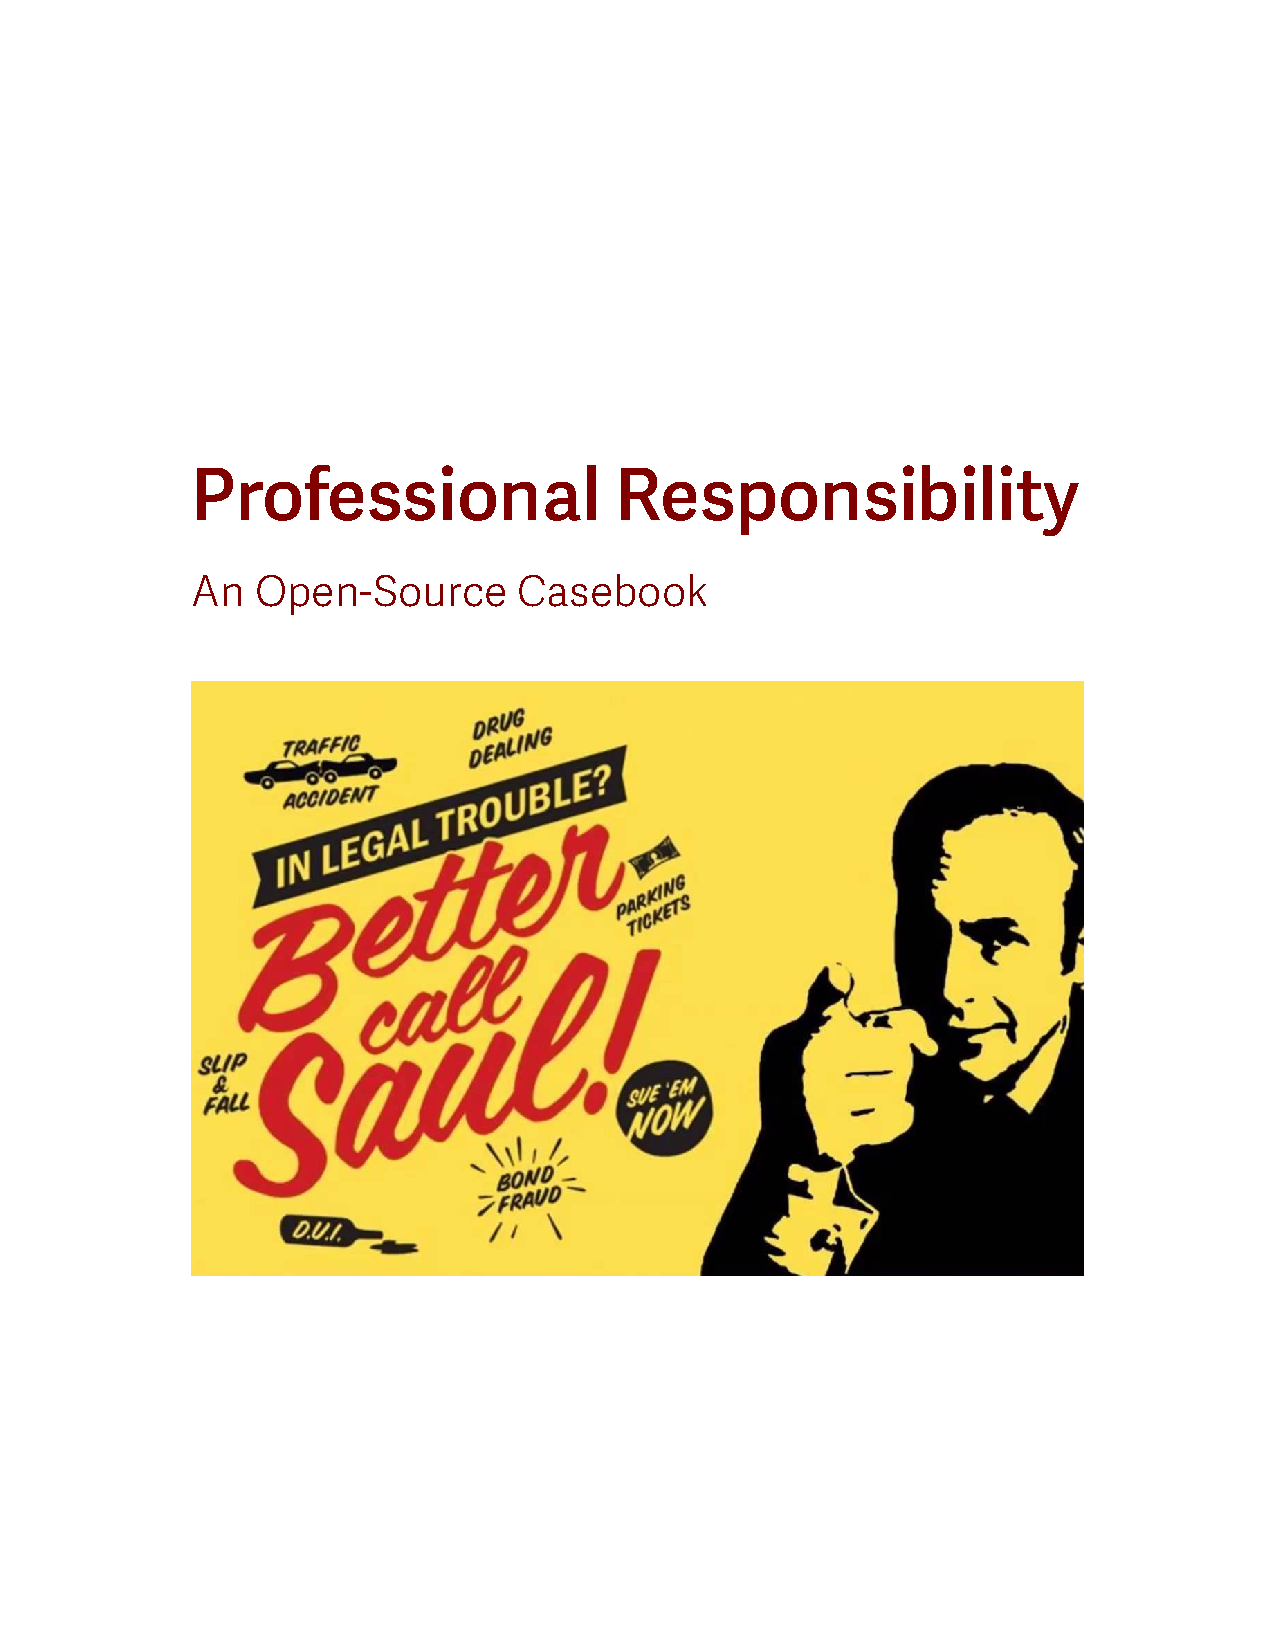
\includepdf{bookcover.pdf}\clearpage}{}

\blankpage

\frontmatter

% Frontispiece
\thispagestyle{empty}

\begin{figure}
\centering
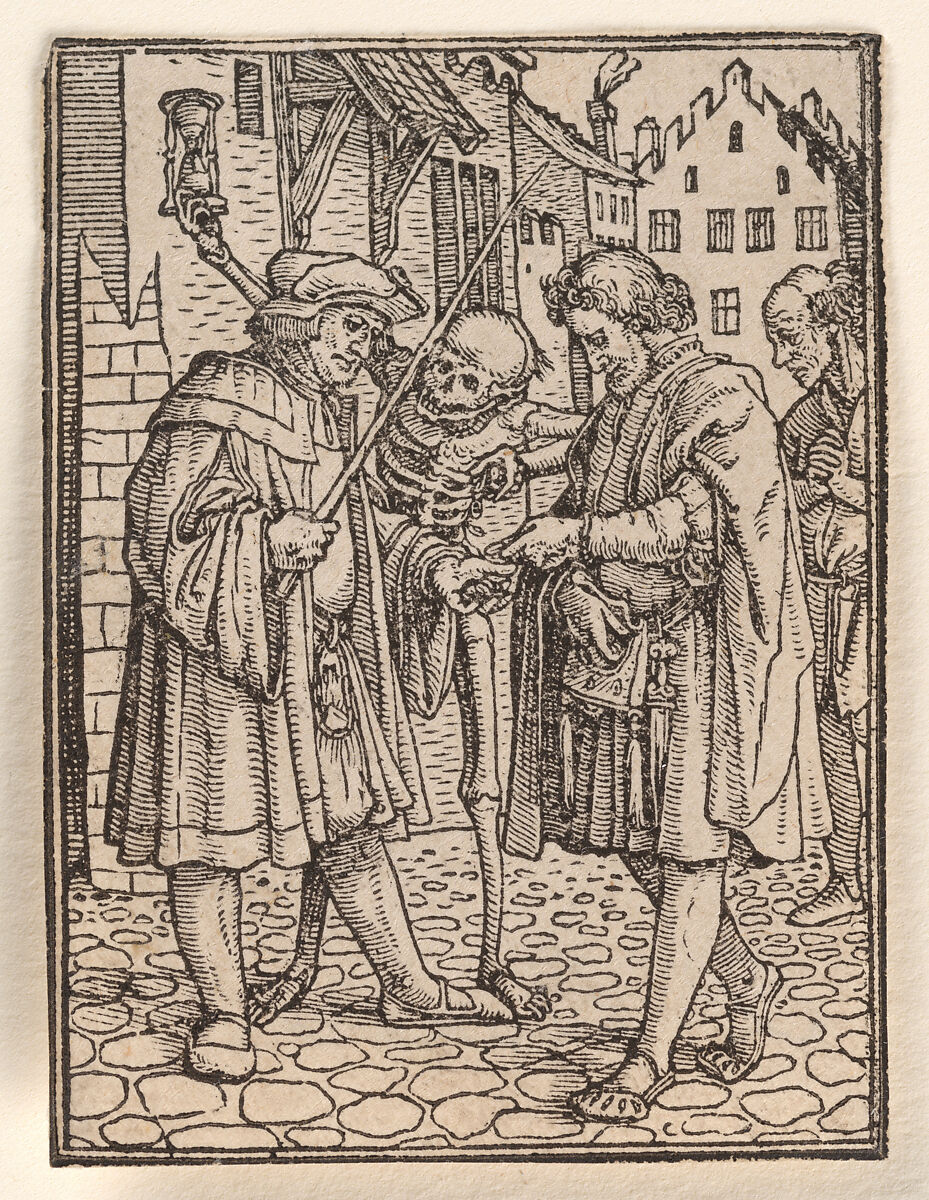
\includegraphics[width=0.9\textwidth]{../img/holbein-advocate.jpg}
\end{figure}

\clearpage

% Title page

\thispagestyle{empty}

\begin{flushright}

\vspace*{50mm}

{\bfseries\Huge{Professional Responsibility}} 

{\bfseries\vspace{5mm}}

{\Large{An Open-Source Casebook}} 

\vspace{20mm}

{\normalsize{Eric M. Fink}} 

\vspace*{\fill}

\begin{small}

\rmfamily{Elon Law School}  

\rmfamily{\textit{Greensboro, North Carolina}}  

\rmfamily{\monthyear} 

\end{small}

\end{flushright}

\clearpage

% License 

\thispagestyle{empty}
\begingroup
\parindent 0pt
\vspace*{\fill}

\ccbyncsa

\begin{small}
\raggedright{This work is licensed under a Creative Commons Attribution-NonCommercial-ShareAlike 4.0 International License.} \\
\url{https://creativecommons.org/licenses/by-nc-sa/4.0/}

\vspace{1em}

Eric M. Fink\\
Associate Professor of Law \\
Elon University School of Law \\
Greensboro, North Carolina 27408 \\
\url{https://www.emfink.net/ElonLaw/}

\vspace{1em}

Source code: \url{https://github.com/EricMFink/PRCasebook}

\itshape{version 4.1, \monthyear}

\end{small}
\endgroup

\clearpage

% Epigraph 

\thispagestyle{empty}

\topskip0pt
\vspace*{\fill}
\openepigraph{I'm seventeen years old, my name is Juan García Madero,
and I'm in my first semester of law school. I wanted to study
literature, not law, but my uncle insisted, and in the end I gave in.
I'm an orphan, and someday I'll be a lawyer. That's what I told my aunt
and uncle, and then I shut myself in my room and cried all
night.}{Roberto Bolaño}{The Savage Detectives}
\vspace*{\fill}

% Preface 
\chapter*{Preface}

This casebook presents material for use in a law school Professional Responsibility course. Topics covered include the organization and regulation of the legal profession, the nature of the attorney-client relationship, and the duties that attorneys owe to clients and others.

Most of the materials reproduced here are in the public domain; excerpts from copyrighted materials are included for teaching purposes under the fair use doctrine. Materials have been redacted to omit passages not pertinent to the learning objectives. Judicial opinions have also been "cleaned up" for ease of reading.\footnote{\textit{See} Jack Metzler, {\textit{Cleaning Up Quotations}}, 18 J. App. Prac. \& Process 143 (2017) (proposing "cleaned up" parenthetical for quotations from judicial opinions, to indicate the author “has removed extraneous, non-substantive material like brackets, quotation marks, ellipses, footnote reference numbers, and internal citations; may have changed capitalization without using brackets to indicate that change; and affirmatively represents that the alterations were made solely to enhance readability and that the quotation otherwise faithfully reproduces the quoted text.”)} 
\renewcommand*\contentsname{Contents}
{
\hypersetup{linkcolor=}
\setcounter{tocdepth}{1}
\tableofcontents
}

\mainmatter
\chapter{Law as a Regulated
Profession}\label{law-as-a-regulated-profession}

\section{Regulatory Authorities}\label{regulatory-authorities}

\subsection{\texorpdfstring{Fred Zacharias, \emph{The Myth of
Self-Regulation}, 93 Minn. L. Rev.~1147
(2009)}{Fred Zacharias, The Myth of Self-Regulation, 93 Minn. L. Rev.~1147 (2009)}}\label{fred-zacharias-the-myth-of-self-regulation-93-minn.-l.-rev.-1147-2009}

Law in the United States is a heavily regulated industry. Lawyers are
licensed in each state. They are governed by profesional rules, usually
adopted and enforced by state supreme courts. The courts regulate
lawyers separately as well, through supervisory decisions in the course
of litigation and by implementing common law civil liability rules that
govern legal practice. These include malpractice, breach of fiduciary
duty, and other causes of action. Administrative agencies---particularly
federal agencies---also establish and implement rules governing lawyers
who practice before them. Federal and state legislatures play a further
role in regulating the bar, providing statutory regulations and criminal
penalties that apply to lawyers.

Nevertheless, courts, commentators, and legal ethics regulators continue
to conceptualize law as a ``self-regulated profession.'' \ldots{} The
preamble to the \ldots{} ABA Model Rules of Professional Conduct
maintains an emphasis on the importance of self-regulation desipite the
fact that the Rules are intended to be adopted as enforceable by state
supreme courts.

\subsection{Model Rules of Professional
Conduct}\label{model-rules-of-professional-conduct}

\subsubsection{Preamble: A Lawyer's
Responsibilities}\label{preamble-a-lawyers-responsibilities}

{[}1{]} A lawyer, as a member of the legal profession, is a
representative of clients, an officer of the legal system and a public
citizen having special responsibility for the quality of justice.

{[}2{]} As a representative of clients, a lawyer performs various
functions. As advisor, a lawyer provides a client with an informed
understanding of the client's legal rights and obligations and explains
their practical implications. As advocate, a lawyer zealously asserts
the client's position under the rules of the adversary system. As
negotiator, a lawyer seeks a result advantageous to the client but
consistent with requirements of honest dealings with others. As an
evaluator, a lawyer acts by examining a client's legal affairs and
reporting about them to the client or to others.

{[}3{]} In addition to these representational functions, a lawyer may
serve as a third-party neutral, a nonrepresentational role helping the
parties to resolve a dispute or other matter. Some of these Rules apply
directly to lawyers who are or have served as third-party neutrals. See,
e.g., Rules 1.12 and 2.4. In addition, there are Rules that apply to
lawyers who are not active in the practice of law or to practicing
lawyers even when they are acting in a nonprofessional capacity. For
example, a lawyer who commits fraud in the conduct of a business is
subject to discipline for engaging in conduct involving dishonesty,
fraud, deceit or misrepresentation. See Rule 8.4.

{[}4{]} In all professional functions a lawyer should be competent,
prompt and diligent. A lawyer should maintain communication with a
client concerning the representation. A lawyer should keep in confidence
information relating to representation of a client except so far as
disclosure is required or permitted by the Rules of Professional Conduct
or other law.

{[}5{]} A lawyer's conduct should conform to the requirements of the
law, both in professional service to clients and in the lawyer's
business and personal affairs. A lawyer should use the law's procedures
only for legitimate purposes and not to harass or intimidate others. A
lawyer should demonstrate respect for the legal system and for those who
serve it, including judges, other lawyers and public officials. While it
is a lawyer's duty, when necessary, to challenge the rectitude of
official action, it is also a lawyer's duty to uphold legal process.

{[}6{]} As a public citizen, a lawyer should seek improvement of the
law, access to the legal system, the administration of justice and the
quality of service rendered by the legal profession. As a member of a
learned profession, a lawyer should cultivate knowledge of the law
beyond its use for clients, employ that knowledge in reform of the law
and work to strengthen legal education. In addition, a lawyer should
further the public's understanding of and confidence in the rule of law
and the justice system because legal institutions in a constitutional
democracy depend on popular participation and support to maintain their
authority. A lawyer should be mindful of deficiencies in the
administration of justice and of the fact that the poor, and sometimes
persons who are not poor, cannot afford adequate legal assistance.
Therefore, all lawyers should devote professional time and resources and
use civic influence to ensure equal access to our system of justice for
all those who because of economic or social barriers cannot afford or
secure adequate legal counsel. A lawyer should aid the legal profession
in pursuing these objectives and should help the bar regulate itself in
the public interest.

{[}7{]} Many of a lawyer's professional responsibilities are prescribed
in the Rules of Professional Conduct, as well as substantive and
procedural law. However, a lawyer is also guided by personal conscience
and the approbation of professional peers. A lawyer should strive to
attain the highest level of skill, to improve the law and the legal
profession and to exemplify the legal profession's ideals of public
service.

{[}8{]} A lawyer's responsibilities as a representative of clients, an
officer of the legal system and a public citizen are usually harmonious.
Thus, when an opposing party is well represented, a lawyer can be a
zealous advocate on behalf of a client and at the same time assume that
justice is being done. So also, a lawyer can be sure that preserving
client confidences ordinarily serves the public interest because people
are more likely to seek legal advice, and thereby heed their legal
obligations, when they know their communications will be private.

{[}9{]} In the nature of law practice, however, conflicting
responsibilities are encountered. Virtually all difficult ethical
problems arise from conflict between a lawyer's responsibilities to
clients, to the legal system and to the lawyer's own interest in
remaining an ethical person while earning a satisfactory living. The
Rules of Professional Conduct often prescribe terms for resolving such
conflicts. Within the framework of these Rules, however, many difficult
issues of professional discretion can arise. Such issues must be
resolved through the exercise of sensitive professional and moral
judgment guided by the basic principles underlying the Rules. These
principles include the lawyer's obligation zealously to protect and
pursue a client's legitimate interests, within the bounds of the law,
while maintaining a professional, courteous and civil attitude toward
all persons involved in the legal system.

{[}10{]} The legal profession is largely self-governing. Although other
professions also have been granted powers of self-government, the legal
profession is unique in this respect because of the close relationship
between the profession and the processes of government and law
enforcement. This connection is manifested in the fact that ultimate
authority over the legal profession is vested largely in the courts.

{[}11{]} To the extent that lawyers meet the obligations of their
professional calling, the occasion for government regulation is
obviated. Self-regulation also helps maintain the legal profession's
independence from government domination. An independent legal profession
is an important force in preserving government under law, for abuse of
legal authority is more readily challenged by a profession whose members
are not dependent on government for the right to practice.

{[}12{]} The legal profession's relative autonomy carries with it
special responsibilities of self-government. The profession has a
responsibility to assure that its regulations are conceived in the
public interest and not in furtherance of parochial or self-interested
concerns of the bar. Every lawyer is responsible for observance of the
Rules of Professional Conduct. A lawyer should also aid in securing
their observance by other lawyers. Neglect of these responsibilities
compromises the independence of the profession and the public interest
which it serves.

{[}13{]} Lawyers play a vital role in the preservation of society. The
fulfillment of this role requires an understanding by lawyers of their
relationship to our legal system. The Rules of Professional Conduct,
when properly applied, serve to define that relationship.

\subsubsection{Scope}\label{scope}

{[}14{]} The Rules of Professional Conduct are rules of reason. They
should be interpreted with reference to the purposes of legal
representation and of the law itself. Some of the Rules are imperatives,
cast in the terms ``shall'' or ``shall not.'' These define proper
conduct for purposes of professional discipline. Others, generally cast
in the term ``may,'' are permissive and define areas under the Rules in
which the lawyer has discretion to exercise professional judgment. No
disciplinary action should be taken when the lawyer chooses not to act
or acts within the bounds of such discretion. Other Rules define the
nature of relationships between the lawyer and others. The Rules are
thus partly obligatory and disciplinary and partly constitutive and
descriptive in that they define a lawyer's professional role. Many of
the Comments use the term ``should.'' Comments do not add obligations to
the Rules but provide guidance for practicing in compliance with the
Rules.

{[}15{]} The Rules presuppose a larger legal context shaping the
lawyer's role. That context includes court rules and statutes relating
to matters of licensure, laws defining specific obligations of lawyers
and substantive and procedural law in general. The Comments are
sometimes used to alert lawyers to their responsibilities under such
other law.

{[}16{]} Compliance with the Rules, as with all law in an open society,
depends primarily upon understanding and voluntary compliance,
secondarily upon reinforcement by peer and public opinion and finally,
when necessary, upon enforcement through disciplinary proceedings. The
Rules do not, however, exhaust the moral and ethical considerations that
should inform a lawyer, for no worthwhile human activity can be
completely defined by legal rules. The Rules simply provide a framework
for the ethical practice of law.

{[}17{]} Furthermore, for purposes of determining the lawyer's authority
and responsibility, principles of substantive law external to these
Rules determine whether a client-lawyer relationship exists. Most of the
duties flowing from the client-lawyer relationship attach only after the
client has requested the lawyer to render legal services and the lawyer
has agreed to do so. But there are some duties, such as that of
confidentiality under Rule 1.6, that attach when the lawyer agrees to
consider whether a client-lawyer relationship shall be established. See
Rule 1.18. Whether a client-lawyer relationship exists for any specific
purpose can depend on the circumstances and may be a question of fact.

{[}18{]} Under various legal provisions, including constitutional,
statutory and common law, the responsibilities of government lawyers may
include authority concerning legal matters that ordinarily reposes in
the client in private client-lawyer relationships. For example, a lawyer
for a government agency may have authority on behalf of the government
to decide upon settlement or whether to appeal from an adverse judgment.
Such authority in various respects is generally vested in the attorney
general and the state's attorney in state government, and their federal
counterparts, and the same may be true of other government law officers.
Also, lawyers under the supervision of these officers may be authorized
to represent several government agencies in intragovernmental legal
controversies in circumstances where a private lawyer could not
represent multiple private clients. These Rules do not abrogate any such
authority.

{[}19{]} Failure to comply with an obligation or prohibition imposed by
a Rule is a basis for invoking the disciplinary process. The Rules
presuppose that disciplinary assessment of a lawyer's conduct will be
made on the basis of the facts and circumstances as they existed at the
time of the conduct in question and in recognition of the fact that a
lawyer often has to act upon uncertain or incomplete evidence of the
situation. Moreover, the Rules presuppose that whether or not discipline
should be imposed for a violation, and the severity of a sanction,
depend on all the circumstances, such as the willfulness and seriousness
of the violation, extenuating factors and whether there have been
previous violations.

{[}20{]} Violation of a Rule should not itself give rise to a cause of
action against a lawyer nor should it create any presumption in such a
case that a legal duty has been breached. In addition, violation of a
Rule does not necessarily warrant any other nondisciplinary remedy, such
as disqualification of a lawyer in pending litigation. The Rules are
designed to provide guidance to lawyers and to provide a structure for
regulating conduct through disciplinary agencies. They are not designed
to be a basis for civil liability. Furthermore, the purpose of the Rules
can be subverted when they are invoked by opposing parties as procedural
weapons. The fact that a Rule is a just basis for a lawyer's
self-assessment, or for sanctioning a lawyer under the administration of
a disciplinary authority, does not imply that an antagonist in a
collateral proceeding or transaction has standing to seek enforcement of
the Rule. Nevertheless, since the Rules do establish standards of
conduct by lawyers, a lawyer's violation of a Rule may be evidence of
breach of the applicable standard of conduct.

{[}21{]} The Comment accompanying each Rule explains and illustrates the
meaning and purpose of the Rule. The Preamble and this note on Scope
provide general orientation. The Comments are intended as guides to
interpretation, but the text of each Rule is authoritative.

\subsection{Model Rules of Professional Conduct, Rule
1.0}\label{model-rules-of-professional-conduct-rule-1.0}

\subsubsection{Terminology}\label{terminology}

(a) ``Belief'' or ``believes'' denotes that the person involved actually
supposed the fact in question to be true. A person's belief may be
inferred from circumstances.

(b) ``Confirmed in writing,'' when used in reference to the informed
consent of a person, denotes informed consent that is given in writing
by the person or a writing that a lawyer promptly transmits to the
person confirming an oral informed consent. See paragraph (e) for the
definition of ``informed consent.'' If it is not feasible to obtain or
transmit the writing at the time the person gives informed consent, then
the lawyer must obtain or transmit it within a reasonable time
thereafter.

(c) ``Firm'' or ``law firm'' denotes a lawyer or lawyers in a law
partnership, professional corporation, sole proprietorship or other
association authorized to practice law; or lawyers employed in a legal
services organization or the legal department of a corporation or other
organization.

(d) ``Fraud'' or ``fraudulent'' denotes conduct that is fraudulent under
the substantive or procedural law of the applicable jurisdiction and has
a purpose to deceive.

(e) ``Informed consent'' denotes the agreement by a person to a proposed
course of conduct after the lawyer has communicated adequate information
and explanation about the material risks of and reasonably available
alternatives to the proposed course of conduct.

(f) ``Knowingly,'' ``known,'' or ``knows'' denotes actual knowledge of
the fact in question. A person's knowledge may be inferred from
circumstances.

(g) ``Partner'' denotes a member of a partnership, a shareholder in a
law firm organized as a professional corporation, or a member of an
association authorized to practice law.

(h) ``Reasonable'' or ``reasonably'' when used in relation to conduct by
a lawyer denotes the conduct of a reasonably prudent and competent
lawyer.

(i) ``Reasonable belief'' or ``reasonably believes'' when used in
reference to a lawyer denotes that the lawyer believes the matter in
question and that the circumstances are such that the belief is
reasonable.

(j) ``Reasonably should know'' when used in reference to a lawyer
denotes that a lawyer of reasonable prudence and competence would
ascertain the matter in question.

(k) ``Screened'' denotes the isolation of a lawyer from any
participation in a matter through the timely imposition of procedures
within a firm that are reasonably adequate under the circumstances to
protect information that the isolated lawyer is obligated to protect
under these Rules or other law.

(l) ``Substantial'' when used in reference to degree or extent denotes a
material matter of clear and weighty importance.

(m) ``Tribunal'' denotes a court, an arbitrator in a binding arbitration
proceeding or a legislative body, administrative agency or other body
acting in an adjudicative capacity. A legislative body, administrative
agency or other body acts in an adjudicative capacity when a neutral
official, after the presentation of evidence or legal argument by a
party or parties, will render a binding legal judgment directly
affecting a party's interests in a particular matter.

(n) ``Writing'' or ``written'' denotes a tangible or electronic record
of a communication or representation, including handwriting,
typewriting, printing, photostating, photography, audio or
videorecording, and electronic communications. A ``signed'' writing
includes an electronic sound, symbol or process attached to or logically
associated with a writing and executed or adopted by a person with the
intent to sign the writing.

\subsection{Note: Judicial, Legislative, \& Administrative
Regulation}\label{note-judicial-legislative-administrative-regulation}

Courts and other tribunals regulate the conduct of attorneys who appear
before them. Court rules and judicial statutes may impose standards of
conduct and authorize the imposition of sanctions on attorneys who
breach those standards. See,
e.g.~\href{https://www.law.cornell.edu/rules/frcp/rule_11}{FRCP Rule 11}
(sanctions for asserting frivilous or bad faith claims, defenses, or
arguments in pleadings and motions);
\href{https://www.law.cornell.edu/rules/frcp/rule_37}{FRCP Rule 37}
(sanctions for failing to make required disclosures or cooperate in
discovery); 28 U.S. Code § 1927 (sactions against ``attorney or other
person admitted to conduct cases in any court of the United States or
any Territory thereof who so multiplies the proceedings in any case
unreasonably and vexatiously'').

In addition to the express authority conferred by statutes or practice
rules, courts possess ``inherent authority'' to regulate the conduct of
attorneys who appear before them. See, e.g., N.C. Gen.~Stat. § 84-36
(``Nothing contained in this Article shall be construed as disabling or
abridging the inherent powers of the court to deal with its
attorneys.'')

Attorney conduct is also subject to legislative and administrative
regulation. Some statutes and agency rules apply specifically to
lawyers, while others apply to certain conduct by lawyers and
non-lawyers alike.

For example, in Section 307 of the Sarbanes-Oxley Act of 2002, Congress
directed the Securities and Exchange Commission to ``issue rules, in the
public interest and for the protection of investors, setting forth
minimum standards of professional conduct for attorneys appearing and
practicing before the Commission in any way in the representation of
issuers.'' The Act specifically calls for rules:

\begin{itemize}
\item
  (1) requiring an attorney to report evidence of a material violation
  of securities law or breach of fiduciary duty or similar violation by
  the company or any agent thereof, to the chief legal counsel or the
  chief executive officer of the company (or the equivalent thereof);
  and
\item
  (2) if the counsel or officer does not appropriately respond to the
  evidence (adopting, as necessary, appropriate remedial measures or
  sanctions with respect to the violation), requiring the attorney to
  report the evidence to the audit committee of the board of directors
  of the issuer or to another committee of the board of directors
  comprised solely of directors not employed directly or indirectly by
  the issuer, or to the board of directors.
\end{itemize}

15 U.S.C. § 7245. The SEC rules set out standards and procedures for
mandatory reporting by attorneys
(\href{https://www.law.cornell.edu/cfr/text/17/part-205}{17 C.F.R. §§
205.3-205.5}). Attorneys who violate those are subject to ``the civil
penalties and remedies for a violation of the federal securities laws
available to the Commission in an action brought by the Commission
thereunder,'' § 205.6(a), as well as disciplinary proceedings by the
Commission,'' which ``may result in an attorney being censured, or being
temporarily or permanently denied the privilege of appearing or
practicing before the Commission,'' § 205.6(b). They ``may also be
subject to discipline for the same conduct in a jurisdiction where the
attorney is admitted or practices.'' § 205.6(b).

\section{Misconduct \& Discipline}\label{misconduct-discipline}

\subsection{N.C. Gen.~Stat. § 84-28}\label{n.c.-gen.-stat.-84-28}

\subsubsection{Discipline and
disbarment.}\label{discipline-and-disbarment.}

(a) Any {\marginnote{\begin{footnotesize}\emph{Council}: ``The North
Carolina State Bar is governed by a 60-member council whose members are
lawyers elected by the lawyers in their home communities, as well a
three nonlawyer members of the council. The public's interests are
represented by three members of the council who are not lawyers and who
are appointed by the governor and other elected officials.''
\href{https://www.ncbar.gov/about-us/leadership/}{NC State
Bar}\end{footnotesize}}} attorney admitted to practice law in this State
is subject to the disciplinary jurisdiction of the Council under such
rules and procedures as the Council shall adopt as provided in G.S.
84-23.

(b) The following acts or omissions by a member of the North Carolina
State Bar or any attorney admitted for limited practice under G.S.
84-4.1, individually or in concert with any other person or persons,
shall constitute misconduct and shall be grounds for discipline whether
the act or omission occurred in the course of an attorney-client
relationship or otherwise:

\begin{itemize}
\item
  (1) Conviction of, or a tender and acceptance of a plea of guilty or
  no contest to, a criminal offense showing professional unfitness;
\item
  (2) The violation of the Rules of Professional Conduct adopted and
  promulgated by the Council in effect at the time of the act;
\item
  (3) Knowing misrepresentation of any facts or circumstances
  surrounding any complaint, allegation or charge of misconduct; failure
  to answer any formal inquiry or complaint issued by or in the name of
  the North Carolina State Bar in any disciplinary matter; or contempt
  of the Council or any committee of the North Carolina State Bar.
\end{itemize}

(c) Misconduct by any attorney shall be grounds for:

\begin{itemize}
\item
  (1) Disbarment;
\item
  (2) Suspension for a period up to but not exceeding five years, any
  portion of which may be stayed upon reasonable conditions to which the
  offending attorney consents;
\item
  (3) Censure - A censure is a written form of discipline more serious
  than a reprimand issued in cases in which an attorney has violated one
  or more provisions of the Rules of Professional Conduct and has caused
  significant harm or potential significant harm to a client, the
  administration of justice, the profession or members of the public,
  but the protection of the public does not require suspension of the
  attorney's license;
\item
  (4) Reprimand - A reprimand is a written form of discipline more
  serious than an admonition issued in cases in which an attorney has
  violated one or more provisions of the Rules of Professional Conduct,
  but the protection of the public does not require a censure. A
  reprimand is generally reserved for cases in which the attorney's
  conduct has caused harm or potential harm to a client, the
  administration of justice, the profession, or members of the public;
  or
\item
  (5) Admonition - An admonition is a written form of discipline imposed
  in cases in which an attorney has committed a minor violation of the
  Rules of Professional Conduct.
\item
  Any order disbarring or suspending an attorney may impose reasonable
  conditions precedent to reinstatement. No attorney who has been
  disbarred by the Disciplinary Hearing Commission, the Council, or by
  order of any court of this State may seek reinstatement to the
  practice of law prior to five years from the effective date of the
  order of disbarment. Any order of the Disciplinary Hearing Commission
  or the Grievance Committee imposing an admonition, reprimand, censure,
  or stayed suspension may also require the attorney to complete a
  reasonable amount of continuing legal education in addition to the
  minimum amount required by the North Carolina Supreme Court.
\end{itemize}

(d) Any attorney admitted to practice law in this State, who is
convicted of or has tendered and has had accepted, a plea of guilty or
no contest to, a criminal offense showing professional unfitness, may be
disciplined based upon the conviction, without awaiting the outcome of
any appeals of the conviction. An order of discipline based solely upon
a conviction of a criminal offense showing professional unfitness shall
be vacated immediately upon receipt by the Secretary of the North
Carolina State Bar of a certified copy of a judgment or order reversing
the conviction. The fact that the attorney's criminal conviction has
been overturned on appeal shall not prevent the North Carolina State Bar
from conducting a disciplinary proceeding against the attorney based
upon the same underlying facts or events that were the subject of the
criminal proceeding.

(d1) An attorney who is disciplined as provided in subsection (d) of
this section may petition the court in the trial division in the
judicial district where the conviction occurred for an order staying the
disciplinary action pending the outcome of any appeals of the
conviction. The court may grant or deny the stay in its discretion upon
such terms as it deems proper. A stay of the disciplinary action by the
court shall not prevent the North Carolina State Bar from going forward
with a disciplinary proceeding against the attorney based upon the same
underlying facts or events that were the subject of the criminal
proceeding.

(e) Any attorney admitted to practice law in this State who is
disciplined in another jurisdiction shall be subject to the same
discipline in this State: Provided, that the discipline imposed in the
other jurisdiction does not exceed that provided for in subsection (c)
above and that the attorney was not deprived of due process in the other
jurisdiction.

(f) Upon application by the North Carolina State Bar, misconduct by an
attorney admitted to practice in this State may be restrained or
enjoined where the necessity for prompt action exists regardless of
whether a disciplinary proceeding in the matter of the conduct is
pending. The application shall be filed in the Superior Court of Wake
County and shall be governed by the procedure set forth in G.S. 1A-1,
Rule 65.

(g) Any member of the North Carolina State Bar may be transferred to
disability inactive status for mental incompetence, physical disability,
or substance abuse interfering with the attorney's ability to
competently engage in the practice of law under the rules and procedures
the Council adopts pursuant to G.S. 84-23.

(h) There shall be an appeal of right by either party from any final
order of the Disciplinary Hearing Commission to the North Carolina Court
of Appeals. Review by the appellate division shall be upon matters of
law or legal inference. The procedures governing any appeal shall be as
provided by statute or court rule for appeals in civil cases. A final
order which imposes disbarment or suspension for 18 months or more shall
not be stayed except upon application, under the rules of the Court of
Appeals, for a writ of supersedeas. A final order imposing suspension
for less than 18 months or any other discipline except disbarment shall
be stayed pending determination of any appeal of right.

(i) The North Carolina State Bar may invoke the process of the General
Court of Justice to enforce the powers of the Council or any committee
to which the Council delegates its authority.

(j) The North Carolina State Bar may apply to appropriate courts for
orders necessary to protect the interests of clients of missing,
suspended, disbarred, disabled, or deceased attorneys.

\begin{itemize}
\tightlist
\item
  The senior regular resident judge of the superior court of any
  district wherein a member of the North Carolina State Bar resides or
  maintains an office shall have the authority and power to enter orders
  necessary to protect the interests of the clients, including the
  authority to order the payment of compensation by the member or the
  estate of a deceased or disabled member to any attorney appointed to
  administer or conserve the law practice of the member. Compensation
  awarded to a member serving under this section awarded from the estate
  of a deceased member shall be considered an administrative expense of
  the estate for purposes of determining priority of payment.
\end{itemize}

\subsection{Model Rules of Professional Conduct, Rule
8.2}\label{model-rules-of-professional-conduct-rule-8.2}

\subsubsection{Judicial \& Legal
Officials}\label{judicial-legal-officials}

(a) A lawyer shall not make a statement that the lawyer knows to be
false or with reckless disregard as to its truth or falsity concerning
the qualifications or integrity of a judge, adjudicatory officer or
public legal officer, or of a candidate for election or appointment to
judicial or legal office.

(b) A lawyer who is a candidate for judicial office shall comply with
the applicable provisions of the Code of Judicial Conduct.

\subsection{Model Rules of Professional Conduct, Rule
8.3}\label{model-rules-of-professional-conduct-rule-8.3}

\subsubsection{Reporting Professional
Misconduct}\label{reporting-professional-misconduct}

(a) A lawyer who knows that another lawyer has committed a violation of
the Rules of Professional Conduct that raises a substantial question as
to that lawyer's honesty, trustworthiness or fitness as a lawyer in
other respects, shall inform the appropriate professional authority.

(b) A lawyer who knows that a judge has committed a violation of
applicable rules of judicial conduct that raises a substantial question
as to the judge's fitness for office shall inform the appropriate
authority.

(c) This Rule does not require disclosure of information otherwise
protected by Rule 1.6 or information gained by a lawyer or judge while
participating in an approved lawyers assistance program.

\subsection{In re Riehlmann, 891 So.2d 1239 (La.
2005)}\label{in-re-riehlmann-891-so.2d-1239-la.-2005}

This disciplinary matter arises from formal charges filed by the Office
of Disciplinary Counsel (``ODC'') against respondent, Michael G.
Riehlmann, an attorney licensed to practice law in Louisiana.

\subsubsection{Underlying Facts}\label{underlying-facts}

Respondent is a criminal defense attorney who was formerly employed as
an Assistant District Attorney in the Orleans Parish District Attorney's
Office. One evening in April 1994, respondent met his close friend and
law school classmate, Gerry Deegan, at a bar near the Orleans Parish
Criminal District Court. Like respondent, Mr.~Deegan had been a
prosecutor in the Orleans Parish District Attorney's Office before he
``switched sides'' in 1987. During their conversation in the bar,
Mr.~Deegan told respondent that he had that day learned he was dying of
colon cancer. In the same conversation, Mr.~Deegan confided to
respondent that he had suppressed exculpatory blood evidence in a
criminal case he prosecuted while at the District Attorney's Office.
Respondent recalls that he was ``surprised'' and ``shocked'' by his
friend's revelation, and that he urged Mr.~Deegan to ``remedy'' the
situation. It is undisputed that respondent did not report Mr.~Deegan's
disclosure to anyone at the time it was made. Mr.~Deegan died in July
1994, having done nothing to ``remedy'' the situation of which he had
spoken in the bar.

Nearly five years after Mr.~Deegan's death, one of the defendants whom
he had prosecuted in a 1985 armed robbery case was set to be executed by
lethal injection on May 20, 1999. In April 1999, the lawyers for the
defendant, John Thompson, discovered a crime lab report which contained
the results of tests performed on a piece of pants leg and a tennis shoe
that were stained with the perpetrator's blood during a scuffle with the
victim of the robbery attempt. The crime lab report concluded that the
robber had Type ``B'' blood. Because Mr.~Thompson has Type ``O'' blood,
the crime lab report proved he could not have committed the robbery;
nevertheless, neither the crime lab report nor the blood-stained
physical evidence had been disclosed to Mr.~Thompson's defense counsel
prior to or during trial. Respondent claims that when he heard about the
inquiry of Mr.~Thompson's lawyers, he immediately realized that this was
the case to which Mr.~Deegan had referred in their April 1994
conversation in the bar. On April 27, 1999, respondent executed an
affidavit for Mr.~Thompson in which he attested that during the 1994
conversation, ``the late Gerry Deegan said to me that he had
intentionally suppressed blood evidence in the armed robbery trial of
John Thompson that in some way exculpated the defendant.''

In May 1999, respondent reported Mr.~Deegan's misconduct to the ODC. In
June 1999, respondent testified in a hearing on a motion for new trial
in Mr.~Thompson's armed robbery case. During the hearing, respondent
testified that Mr.~Deegan had told him that he ``suppressed exculpatory
evidence that was blood evidence, that seemed to have excluded
Mr.~Thompson as the perpetrator of an armed robbery.'' Respondent also
admitted that he ``should have reported'' Mr.~Deegan's misconduct, and
that while he ultimately did so, ``I should have reported it sooner, I
guess.''

On September 30, 1999, respondent gave a sworn statement to the ODC in
which he was asked why he did not report Mr.~Deegan's disclosure to
anyone at the time it was made. Respondent replied:

\begin{quote}
I think that under ordinary circumstances, I would have. I really
honestly think I'm a very good person. And I think I do the right thing
whenever I'm given the opportunity to choose. This was unquestionably
the most difficult time of my life. Gerry, who was like a brother to me,
was dying. And that was, to say distracting would be quite an
understatement. I'd also left my wife just a few months before, with
three kids, and was under the care of a psychiatrist, taking
antidepressants. My youngest son was then about two and had just
recently undergone open-heart surgery. I had a lot on my plate at the
time. A great deal of it of my own making; there's no question about it.
But, nonetheless, I was very, very distracted, and I simply did not give
it the important consideration that it deserved. But it was a very
trying time for me. And that's the only explanation I have, because,
otherwise, I would have reported it immediately had I been in a better
frame of mind.
\end{quote}

\subsubsection{Disciplinary Proceedings}\label{disciplinary-proceedings}

\paragraph{Formal Charges}\label{formal-charges}

On January 4, 2001, the ODC filed one count of formal charges against
respondent, alleging that his failure to report his unprivileged
knowledge of Mr.~Deegan's prosecutorial misconduct violated Rules 8.3(a)
(reporting professional misconduct), 8.4(c) (engaging in conduct
involving dishonesty, fraud, deceit, or misrepresentation), and 8.4(d)
(engaging in conduct prejudicial to the administration of justice) of
the Rules of Professional Conduct. The ODC subsequently amended the
formal charges to delete the alleged violation of Rule 8.4(c).

On March 5, 2002, respondent answered the amended formal charges and
admitted some of the factual allegations therein, but denied that his
conduct violated the Rules of Professional Conduct. Specifically,
respondent asserted that Rule 8.3(a) ``merely requires that an attorney
possessing unprivileged knowledge of a violation of this Code shall
report such knowledge to the authority empowered to investigate such
acts. It is undisputed that respondent did report his knowledge of
Deegan's statements to Thompson's attorneys, with the clear
understanding that this information would be reported to the District
Attorney and the Court, undeniably authorities empowered to investigate
Deegan's conduct.''

\paragraph{Formal Hearing}\label{formal-hearing}

When this matter proceeded to a formal hearing before the committee,
respondent testified that his best recollection of his conversation with
Mr.~Deegan in 1994 ``is that he told me that he did not turn over
evidence to his opponents that might have exculpated the defendant.''
Nevertheless, when asked whether he recognized during the barroom
conversation that Mr.~Deegan had violated his ethical duties, respondent
replied, ``Well, certainly.'' Respondent admitted that he gave the
conversation no further thought after he left the bar because he was
``distracted'' by his own personal problems.

\paragraph{Hearing Committee
Recommendation}\label{hearing-committee-recommendation}

In its report filed with the disciplinary board, the hearing committee
concluded that respondent did not violate Rule 8.3(a), but that he
should be publicly reprimanded for his violation of Rule 8.4(d).

Considering the evidence presented at the hearing, the committee made a
factual finding that during the 1994 barroom conversation, Mr.~Deegan
explained to respondent that he did not turn over evidence in a case
that might have exculpated a defendant, but ``equivocated on whether the
evidence proved the innocence of a defendant.'' Moreover, the committee
found there is no clear and convincing evidence that Mr.~Deegan
identified John Thompson by name in the disclosure to respondent in
1994. The committee believed respondent's testimony that he did not draw
a connection between Mr.~Deegan's 1994 statements and the Thompson case
until 1999, when he heard about the inquiry of Mr.~Thompson's lawyers.

Based on its factual findings, the committee found that respondent did
not violate Rule 8.3(a) because he did not have ``knowledge of a
violation'' that obligated him to report Mr.~Deegan to the ODC or to any
other authority. The committee pointed out that it believed respondent's
testimony that Mr.~Deegan made equivocal statements in 1994 that did not
rise to the level of a ``confession'' that Deegan had actually
suppressed the crime lab report nine years earlier. The committee found
Mr.~Deegan qualified his statement that the evidence ``might'' have
exculpated the defendant, and furthermore, agreed that if the evidence
did not tend to negate the defendant's guilt, Mr.~Deegan would have had
no obligation to turn over that evidence under \emph{Brady}.
Consequently, the committee determined that respondent would have had no
violation to report. The committee found Mr.~Deegan's statements at most
suggested a potential violation of the ethical rules, but the committee
declined to construe Rule 8.3(a) to require a lawyer to report a
potential violation of an ethical rule by another lawyer.

Although the committee did not find that respondent violated Rule
8.3(a), the committee found he violated Rule 8.4(d), which imposes a
``broader obligation to ensure that justice is fairly administered,'' by
his ``complete inaction after the barroom disclosure.'' The committee
found respondent's conversation with Mr.~Deegan ``was of sufficient
importance that not pursuing Deegan for a disclosure or to rectify the
situation, failing to investigate further, and ultimately not taking any
affirmative action for five years constituted conduct that hindered the
administration of justice.'' The committee determined the baseline
sanction for such conduct by respondent is a reprimand.

As aggravating factors, the committee recognized respondent's experience
in the practice of law (admitted 1983) and the vulnerability of the
victim, Mr.~Thompson. In mitigation, the committee acknowledged the
absence of a prior disciplinary record, absence of a dishonest or
selfish motive, personal or emotional problems (including the terminal
colon cancer of his best friend, Mr.~Deegan; marital problems; and the
health problems both he and his son were experiencing), timely good
faith effort to rectify the consequences of Mr.~Deegan's misconduct,
full and free disclosure to the disciplinary board and a cooperative
attitude toward the proceeding, character and reputation, and remorse.

In light of the mitigating factors present, and finding that a
suspension would serve no useful purpose in this case, the committee
recommended the imposition of a public reprimand.

Both respondent and the ODC filed objections to the hearing committee's
recommendation.

\paragraph{Disciplinary Board
Recommendation}\label{disciplinary-board-recommendation}

The disciplinary board adopted the hearing committee's factual findings
but rejected its application of Rule 8.3(a) of the Rules of Professional
Conduct. The board determined that a finding of a violation of Rule
8.3(a) requires clear and convincing evidence that an attorney (1)
possessed unprivileged knowledge of an ethical violation and (2) failed
to report such knowledge to a tribunal or other authority empowered to
investigate or act upon such violation. Concerning the knowledge
requirement, the board considered various legal authorities interpreting
both Louisiana Rule 8.3(a) and Model Rule 8.3(a), and determined that a
lawyer's duty to report professional misconduct is triggered when, under
the circumstances, a reasonable lawyer would have ``a firm opinion that
the conduct in question more likely than not occurred.'' The board
explained that the requisite knowledge under Rule 8.3(a) is ``more than
a mere suspicion, but less than absolute or moral certainty.''

Employing this analysis, the board concluded the committee erred in its
finding that respondent had no duty to report because Mr.~Deegan's
statements were equivocal. The board found respondent must have
understood from his 1994 conversation with Mr.~Deegan that Mr.~Deegan
had suppressed Brady evidence:

\begin{quote}
If Respondent did not understand from his conversation with Deegan that
Deegan has suppressed evidence that he was obligated to produce, why was
Respondent shocked and surprised? Why did Respondent tell Deegan that
what he had done was ``not right'' and that Deegan had to ``rectify''
the situation? Respondent never changed his testimony in this respect.
Obviously, if Respondent understood from his conversation with Deegan
that Deegan had done nothing wrong, there would have been no occasion
for Respondent to say that it was ``not right'' or that Deegan had to
``rectify'' what he had done. The Committee makes no attempt to explain
these circumstances which are wholly inconsistent with the Committee's
theory. This uncontradicted circumstantial evidence cannot be ignored.
Indeed, if Deegan believed he had done nothing wrong, why did Deegan
even bother to bring the matter up nearly ten (10) years after Thompson
was convicted? More importantly, why did he bring it up in the same
conversation that he disclosed to Respondent that he (Deegan) had
terminal colon cancer?
\end{quote}

The board concluded that a reasonable lawyer under the circumstances
would have formed a firm opinion that Mr.~Deegan had wrongfully failed
to disclose the blood evidence, and that respondent did in fact form
such an opinion because he advised Mr.~Deegan that what he (Deegan) did
was ``not right'' and that he (Deegan) had to ``rectify'' the situation.
Accordingly, the board found respondent had sufficient knowledge of
misconduct by Mr.~Deegan to trigger a duty to report the misconduct to
the disciplinary authorities.

The board then turned to a discussion of whether respondent's failure to
report Mr.~Deegan's misconduct for more than five years after learning
of it constituted a failure to report under Rule 8.3(a). The board
acknowledged that Rule 8.3(a) does not provide any specific time limit
or period within which the misconduct must be reported. Nevertheless,
the board reasoned that Rule 8.3(a) serves no useful purpose unless it
is read to require reporting to an appropriate authority within a
reasonable time under the circumstances. Therefore, absent special
circumstances, the board determined that a lawyer must report his
knowledge of misconduct ``promptly.'' Applying these principles to the
instant case, the board determined respondent's disclosure in 1999 of
misconduct he discovered in 1994 was not timely and did not satisfy the
requirements of Rule 8.3(a).

The board also found that respondent's conduct violated Rule 8.4(d)
because his inactivity following Mr.~Deegan's disclosure was prejudicial
to the administration of justice.

The board found respondent knowingly violated a duty owed to the
profession, and that his actions resulted in both actual and potential
injury to Mr.~Thompson. The board noted that if respondent had taken
further action in 1994, when Mr.~Deegan made his confession,
Mr.~Thompson's innocence in connection with the armed robbery charge may
have been established sooner. The board also observed that negative
publicity attached to respondent's actions, thereby causing harm to the
legal profession. The board determined the baseline sanction for
respondent's conduct is a suspension from the practice of law.

The board adopted the aggravating and mitigating factors cited by the
hearing committee, except that the board refused to credit respondent
with the mitigating factor of making a timely good faith effort to
rectify the consequences of Mr.~Deegan's misconduct.

The board determined that some period of suspension is appropriate for
respondent's conduct. In light of the significant mitigating factors in
this matter, the board recommended that respondent be suspended from the
practice of law for six months. One board member dissented and would
recommend a suspension of at least one year and one day.

Both respondent and the ODC filed objections to the disciplinary board's
recommendation.

\subsubsection{Discussion}\label{discussion}

In this matter we are presented for the first time with an opportunity
to delineate the scope of an attorney's duty under Rule 8.3 to report
the professional misconduct of a fellow member of the bar. Therefore, we
begin our discussion with a few observations relating to the rule and
its history.

The American legal profession has long recognized the necessity of
reporting lawyers' ethical misconduct. When the American Bar Association
adopted its first code of ethics in 1908, Canon 29 of the Canons of
Professional Ethics, entitled ``Upholding the Honor of the Profession,''
encouraged lawyers to ``expose without fear or favor before the proper
tribunals corrupt or dishonest conduct in the profession''. More than
sixty years later, the ABA enacted Disciplinary Rule 1-103(A) of the
Model Code of Professional Responsibility, the predecessor of the
current Rule 8.3(a) of the Model Rules of Professional Conduct. Both the
1969 Code, in DR 1-103(A), and the 1983 Model Rules, in Rule 8.3(a),
make it clear that the duty to report is not merely an aspiration but is
mandatory, the violation of which subjects the lawyer to discipline.

This court first adopted Rule 8.3 on December 18, 1986, effective
January 1, 1987. Louisiana's rule is based on ABA Model Rule 8.3;
however, there are several differences between the Model Rule and the
Louisiana Rule that was in effect in 2001, at the time the formal
charges were filed in this case. Most significantly, Model Rule 8.3
requires a lawyer to report the misconduct of another lawyer only when
the conduct in question ``raises a substantial question'' as to that
lawyer's fitness to practice. Louisiana's version of Rule 8.3 imposed a
substantially more expansive reporting requirement, in that our rule
required a lawyer to report all unprivileged knowledge of any ethical
violation by a lawyer, whether the violation was, in the reporting
lawyer's view, flagrant and substantial or minor and technical. A task
force of the Louisiana State Bar Association concluded that it was
inappropriate to put a lawyer ``in the position of making a subjective
judgment'' regarding the significance of a violation, and felt it was
preferable instead ``to put the burden on every lawyer to report all
violations, regardless of their nature or kind, whether or not they
raised a substantial question as to honesty, trustworthiness, or
fitness.''

We now turn to a more in-depth examination of the reporting requirement
in Louisiana. At the time the formal charges were filed in this case,
Louisiana Rule 8.3(a) provided:

\begin{quote}
A lawyer possessing unprivileged knowledge of a violation of this code
shall report such knowledge to a tribunal or other authority empowered
to investigate or act upon such violation.
\end{quote}

Thus, the rule has three distinct requirements: (1) the lawyer must
possess unprivileged knowledge of a violation of the Rules of
Professional Conduct; (2) the lawyer must report that knowledge; and (3)
the report must be made to a tribunal or other authority empowered to
investigate or act on the violation. We will discuss each requirement in
turn.

\paragraph{Knowledge}\label{knowledge}

In its recommendation in this case, the disciplinary board did excellent
work in collecting and analyzing the cases and legal commentary
interpreting the knowledge requirement of Rule 8.3(a). We need not
repeat that analysis here. Considering those authorities, it is clear
that absolute certainty of ethical misconduct is not required before the
reporting requirement is triggered. The lawyer is not required to
conduct an investigation and make a definitive decision that a violation
has occurred before reporting; that responsibility belongs to the
disciplinary system and this court. On the other hand, knowledge
requires more than a mere suspicion of ethical misconduct. We hold that
a lawyer will be found to have knowledge of reportable misconduct, and
thus reporting is required, where the supporting evidence is such that a
reasonable lawyer under the circumstances would form a firm belief that
the conduct in question had more likely than not occurred. As such,
knowledge is measured by an objective standard that is not tied to the
subjective beliefs of the lawyer in question.

\paragraph{When to Report}\label{when-to-report}

Once the lawyer decides that a reportable offense has likely occurred,
reporting should be made promptly. The need for prompt reporting flows
from the need to safeguard the public and the profession against future
wrongdoing by the offending lawyer. This purpose is not served unless
Rule 8.3(a) is read to require timely reporting under the circumstances
presented.

\paragraph{Appropriate Authority}\label{appropriate-authority}

Louisiana Rule 8.3(a) requires that the report be made to ``a tribunal
or other authority empowered to investigate or act upon such
violation.'' The term ``tribunal or other authority'' is not
specifically defined. However, as the comments to Model Rule 8.3(a)
explain, the report generally should be made to the bar disciplinary
authority. Therefore, a report of misconduct by a lawyer admitted to
practice in Louisiana must be made to the Office of Disciplinary
Counsel.

\subsubsection{Determination of Respondent's Misconduct and Appropriate
Discipline}\label{determination-of-respondents-misconduct-and-appropriate-discipline}

Applying the principles set forth above to the conduct of respondent in
the instant case, we find the ODC proved by clear and convincing
evidence that respondent violated Rule 8.3(a). First, we find that
respondent should have known that a reportable event occurred at the
time of his 1994 barroom conversation with Mr.~Deegan. Stated another
way, respondent's conversation with Mr.~Deegan at that time gave him
sufficient information that a reasonable lawyer under the circumstances
would have formed a firm opinion that the conduct in question more
likely than not occurred. Regardless of the actual words Mr.~Deegan said
that night, and whether they were or were not ``equivocal,'' respondent
understood from the conversation that Mr.~Deegan had done something
wrong. Respondent admitted as much in his affidavit, during the hearing
on the motion for new trial in the criminal case, during his sworn
statement to the ODC, and during his testimony at the formal hearing.
Indeed, during the sworn statement respondent conceded that he would
have reported the matter ``immediately'' were it not for the personal
problems he was then experiencing. Respondent also testified that he was
surprised and shocked by his friend's revelation, and that he told him
to remedy the situation. There would have been no reason for respondent
to react in the manner he did had he not formed a firm opinion that the
conduct in question more likely than not occurred. The circumstances
under which the conversation took place lend further support to this
finding. On the same day that he learned he was dying of cancer,
Mr.~Deegan felt compelled to tell his best friend about something he had
done in a trial that took place nine years earlier. It simply defies
logic that respondent would now argue that he could not be sure that
Mr.~Deegan actually withheld Brady evidence because his statements were
vague and non-specific.

We also find that respondent failed to promptly report Mr.~Deegan's
misconduct to the disciplinary authorities. As respondent himself
acknowledged, he should have reported Mr.~Deegan's statements sooner
than he did. There was no reason for respondent to have waited five
years to tell the ODC about what his friend had done.

In his answer to the formal charges, respondent asserts that he did
comply with the reporting requirement of Rule 8.3(a) because he promptly
reported Mr.~Deegan's misconduct to the District Attorney and the
Criminal District Court through the attorneys for the criminal
defendant, John Thompson. Respondent has misinterpreted Rule 8.3(a) in
this regard. The word ``tribunal'' must be read in the context of the
entire sentence in which it appears. The proper inquiry, therefore, is
what authority is ``empowered'' to act upon a charge of attorney
misconduct. In Louisiana, only this court possesses the authority to
define and regulate the practice of law, including the discipline of
attorneys. In turn, we have delegated to disciplinary counsel the
authority to investigate and prosecute claims of attorney misconduct.
Furthermore, while a trial court bears an independent responsibility to
report attorney misconduct to the ODC, only this court may discipline an
attorney found guilty of unethical behavior. Therefore, respondent is
incorrect in arguing that he discharged his reporting duty under Rule
8.3(a) by reporting Mr.~Deegan's misconduct to Mr.~Thompson's attorneys,
the District Attorney, and/or the Criminal District Court. It is
undisputed that respondent did not report to the appropriate entity, the
ODC, until 1999. That report came too late to be construed as
``prompt.''

Having found professional misconduct, we now turn to a discussion of an
appropriate sanction. In considering that issue, we are mindful that the
purpose of disciplinary proceedings is not primarily to punish the
lawyer, but rather to maintain the appropriate standards of professional
conduct, to preserve the integrity of the legal profession, and to deter
other lawyers from engaging in violations of the standards of the
profession. The discipline to be imposed depends upon the facts of each
case and the seriousness of the offenses involved, considered in light
of any aggravating and mitigating circumstances.

Respondent's actions violated the general duty imposed upon attorneys to
maintain and preserve the integrity of the bar. While we adhere to our
observation in \emph{Brigandi} that an attorney's failure to comply with
the reporting requirement is a ``serious offense,'' in the instant case,
we find that respondent's conduct was merely negligent. Accordingly,
Standard 7.3 of the ABA's \emph{Standards for Imposing Lawyer Sanctions}
provides that the appropriate baseline sanction is a reprimand.

The only aggravating factor present in this case is respondent's
substantial experience in the practice of law. As for mitigating
factors, we adopt those recognized by the disciplinary board, placing
particular emphasis on the absence of any dishonest or selfish motive on
respondent's part. Notwithstanding these factors, however, respondent's
failure to report Mr.~Deegan's bad acts necessitates that some sanction
be imposed. Respondent's knowledge of Mr.~Deegan's conduct was
sufficient to impose on him an obligation to promptly report Mr.~Deegan
to the ODC. Having failed in that obligation, respondent is himself
subject to punishment. Under all of the circumstances presented, we
conclude that a public reprimand is the appropriate sanction.

Accordingly, we will reprimand respondent for his actions.

\subsection{Model Rules of Professional Conduct, Rule
8.4}\label{model-rules-of-professional-conduct-rule-8.4}

\subsubsection{Misconduct}\label{misconduct}

It is professional misconduct for a lawyer to:

(a) violate or attempt to violate the Rules of Professional Conduct,
knowingly assist or induce another to do so, or do so through the acts
of another;

(b) commit a criminal act that reflects adversely on the lawyer's
honesty, trustworthiness or fitness as a lawyer in other respects;

(c) engage in conduct involving dishonesty, fraud, deceit or
misrepresentation;

(d) engage in conduct that is prejudicial to the administration of
justice;

(e) state or imply an ability to influence improperly a government
agency or official or to achieve results by means that violate the Rules
of Professional Conduct or other law;

(f) knowingly assist a judge or judicial officer in conduct that is a
violation of applicable rules of judicial conduct or other law; or

(g) engage in conduct that the lawyer knows or reasonably should know is
harassment or discrimination on the basis of race, sex, religion,
national origin, ethnicity, disability, age, sexual orientation, gender
identity, marital status or socioeconomic status in conduct related to
the practice of law. This paragraph does not limit the ability of a
lawyer to accept, decline or withdraw from a representation in
accordance with Rule 1.16. This paragraph does not preclude legitimate
advice or advocacy consistent with these Rules.

\subsection{Disciplinary Counsel v. Blakeslee, 2023 Ohio 4202
(2023)}\label{disciplinary-counsel-v.-blakeslee-2023-ohio-4202-2023}

Respondent, Jack Allen Blakeslee, of Caldwell, Ohio, was admitted to the
practice of law in Ohio in 1976. In a November 2022 complaint, relator,
disciplinary counsel, charged Blakeslee with professional misconduct for
throwing a feces-filled Pringles can into the parking lot of a
victim-advocacy center involved in a capital-murder case in which
Blakeslee was representing the defendant. Blakeslee waived a
probable-cause determination and, in his answer, admitted many of
relator's factual allegations and the single alleged rule violation. The
parties also submitted joint stipulations of fact, misconduct, and
aggravating and mitigating factors.

After conducting a hearing, a panel of the Board of Professional Conduct
issued a report finding by clear and convincing evidence that Blakeslee
had committed the charged misconduct and recommending that we publicly
reprimand him for that misconduct. The board adopted the panel's
findings and recommendation. For the reasons that follow, we adopt the
board's finding of misconduct but suspend Blakeslee from the practice of
law for one year with six months stayed on the condition that he engage
in no further misconduct.

\subsubsection{MISCONDUCT}\label{misconduct-1}

On June 1, 2021, Alexander Wells was indicted in the Guernsey County
Court of Common Pleas for various offenses, including aggravated murder.
The aggravated-murder offense included a specification that the victim
was under the age of 13, making it a capital offense.

On June 7, 2021, Blakeslee appeared at Wells's arraignment and was
formally appointed by the court to represent him. Victim advocate
Michelle Carpenter Wilkinson, whom had known Blakeslee professionally
for many years, also attended Wells's arraignment. Blakeslee and
Carpenter Wilkinson, who serves as chief executive officer of Haven of
Hope, a victim-advocacy center in Cambridge, attended several additional
court proceedings in the Wells case between June 11 and September 30,
2021.

The trial court scheduled another pretrial hearing in Wells's case for
November 30, 2021, at 8:30 a.m. Before leaving his home on the morning
of that hearing, Blakeslee deposited his feces into an empty Pringles
can. He then drove approximately 20 minutes from his home in Coal Ridge
to Cambridge with the open can of feces. Between 8:10 and 8:15 a.m.,
Blakeslee turned his vehicle down an alley where the Haven of Hope
parking lot is located, approximately two-tenths of a mile from the
Guernsey County Common Pleas courthouse. A sign on the building at the
entrance to the alley indicated ``Haven of Hope Administrative Offices''
above a bold arrow pointing down the alley. Surveillance video shows
that Blakeslee slowed his vehicle as he initially passed Haven of Hope's
parking lot. He continued driving further down the alley, passing
several other parking lots, before turning around. He slowed again as he
passed Haven of Hope's parking lot a second time, threw the Pringles can
containing his feces into the lot, and then drove to the courthouse for
the 8:30 a.m. pretrial hearing in Wells's case.

Carpenter Wilkinson saw Blakeslee throw the can out his vehicle toward
the Haven of Hope parking lot. After Blakeslee drove away, Carpenter
Wilkson approached the item and discovered that it was a Pringles can
containing what appeared to be human feces. She then left for the
courthouse to attend Wells's pretrial hearing. Upon arriving at the
courthouse, she noticed that Blakeslee was also present for the hearing.

Later that day, after discussing the matter with a prosecutor assigned
to the Wells case, Carpenter Wilkinson filed a report with the Cambridge
Police Department. Thereafter, Blakeslee was charged with and pleaded
guilty to minor-misdemeanor charges of disorderly conduct and littering.
He ultimately paid \$248 in fines and court costs for those offenses.

During his disciplinary hearing, Blakeslee testified that he had engaged
in similar misconduct on at least ten other occasions that year and that
he randomly chose the locations where he deposited the Pringles cans
containing his feces. He also specifically denied having any knowledge
that the parking lot in question belonged to Haven of Hope when he threw
the can from his vehicle on November 30, 2021.

The parties stipulated and the board found that Blakeslee's conduct
violated Prof.Cond.R. 8.4(h) (prohibiting a lawyer from engaging in
conduct that adversely reflects on the lawyer's fitness to practice
law).

We adopt that finding of misconduct and expressly find that Blakeslee's
conduct adversely reflects on his fitness to practice law even though
that conduct is not expressly prohibited by another rule.

\subsubsection{RECOMMENDED SANCTION}\label{recommended-sanction}

When imposing sanctions for attorney misconduct, we consider all
relevant factors, including the ethical duties that the lawyer violated,
the aggravating and mitigating factors listed in Gov.Bar R. V(13), and
the sanctions imposed in similar cases.

As for aggravating factors, the parties stipulated that Blakeslee had
engaged in a pattern of misconduct, presumably based on his admission
that he threw feces-filled Pringles cans from his vehicle on at least
ten other occasions. The board disagreed, noting that ``a `pattern of
misconduct,' is typically found where a respondent engages in multiple
acts of misconduct, thus forming a pattern.'' Finding that this case
involved just one rule violation arising from a single incident of
misconduct---and that there was no evidence to establish the
circumstances surrounding the additional instances of misconduct that
Blakeslee had admitted in his testimony---the board rejected the
parties' stipulated aggravating factor. We, however, accept the parties'
stipulation that Blakeslee engaged in a pattern of misconduct.
Regardless of whether Blakeslee randomly deposited the additional cans
of feces or targeted particular locations or individuals, he freely
admitted that he had engaged in similar acts of misconduct on multiple
other occasions.

As for mitigating factors, the parties stipulated to the absence of a
prior disciplinary record, and the board found that Blakeslee has had a
distinguished criminal-defense trial practice for more than four decades
with no prior discipline. In addition, the parties stipulated and the
board found that Blakeslee also had made full and free disclosure to the
board and demonstrated a cooperative attitude toward the disciplinary
proceedings, presented evidence of his good character and reputation,
and had other penalties and sanctions imposed for his
misconduct---namely, the nominal fines and court costs imposed for his
misdemeanor convictions. The board also found that neither Wells nor
Carpenter Wilkinson had been harmed by Blakeslee's actions.

In addition, the board found that Blakeslee had accepted full
responsibility for his actions, expressed genuine remorse, and testified
that he is no longer engaging in the misconduct. Although Blakeslee
testified that he was a Vietnam veteran and that he had received
psychological treatment for posttraumatic stress disorder (``PTSD'')
related to his military service as well as child abuse, he did not seek
to establish his disorder as a mitigating factor under Gov.Bar R.
V(13)(C)(7).

Blakeslee has described his misconduct as a ``prank'' and admitted that
it was ``stupid.'' He also acknowledged that he was embarrassed by the
public revelation of his misconduct and the resulting media attention.

Relator took the position that Blakeslee deposited the can of feces in
the Haven of Hope parking lot with the intent of targeting Haven of
Hope. In support of this position, relator relied on circumstantial
evidence, including Blakeslee's 20-minute drive, the sign pointing
toward access to Haven of Hope's office, Blakeslee's slow drive down the
alley, and the fact that he went to court immediately after he deposited
the can of feces to attend a hearing in the Wells case where Carpenter
Wilkinson would be present. However, Blakeslee denied having any
knowledge of Haven of Hope's location on November 30, 2021, and
maintained that he had chosen all the locations for his deposits at
random. The hearing panel and the board found Blakeslee's testimony to
be credible and concluded that relator's position was not supported by
clear and convincing evidence.

During closing argument, relator argued that Blakeslee's misconduct
warrants a conditionally stayed six-month suspension whereas Blakeslee
suggested that a public reprimand would be appropriate. Both parties
acknowledged that very few, if any, prior cases offer guidance regarding
the appropriate sanction for the misconduct at issue here.

Relying primarily on \emph{Columbus Bar Assn. v. Linnen,} 2006 Ohio 5480
(2006), \emph{Butler Cty. Bar Assn. v. Blauvelt,} 2020 Ohio 3325 (2020),
and the precept that the primary purpose of the disciplinary sanction is
not to punish the offender but to protect the public, the board
recommends that we publicly reprimand Blakeslee for his misconduct.

Over a period of nearly two years, Linnen approached at least 30
different women throughout Franklin County wearing only athletic shoes
and a stocking cap and photographed their reactions. He admitted that he
would sometimes tap or pinch a victim's rear end to get her attention
and that he may have masturbated in front of his first couple of
victims. Linnen pleaded guilty to 53 misdemeanor offenses---two
first-degree misdemeanor counts of sexual imposition, one first-degree
misdemeanor count of aggravated trespass, 11 third-degree misdemeanor
counts of sexual imposition, and 39 fourth-degree misdemeanor counts of
public indecency. He was sentenced to 18 months of work release, fined
\$3,000, and ordered to continue counseling. We found that Linnen
violated professional-conduct rules prohibiting attorneys from engaging
in illegal conduct involving moral turpitude and conduct that adversely
reflects on a lawyer's fitness to practice.

In aggravation, we found that Linnen had engaged in a pattern of
misconduct involving multiple offenses and that he had acted with a
dishonest or selfish motive, the latter finding based on his testimony
that the impetus for his crimes was ``definitely an adrenaline rush or
euphoria very much like a powerful drug.'' We also found that Linnen had
failed to genuinely acknowledge the wrongful nature of his misconduct,
focusing primarily on his own embarrassment and hardship rather than the
harm he had caused to his victims. In mitigation, Linnen had no prior
disciplinary record, had cooperated completely in the disciplinary
process, and had presented evidence of his good character. We
indefinitely suspended him for his misconduct.

In \emph{Blauvelt,} the attorney was twice caught driving naked. The
first time, he was stopped for a headlight violation and the officer
observed he was naked but filed no charges against him. The second time,
after receiving a report that a motorist was masturbating while driving,
a state trooper stopped Blauvelt's vehicle and found him naked with
pants covering his lap. Blauvelt was charged with public indecency and
operating a vehicle while under the influence; he later pleaded guilty
to public indecency and an amended charge of reckless operation of a
vehicle. He was sentenced to suspended jail terms and ordered to pay
fines, complete a driver-intervention program, and serve a one-year term
of nonreporting probation.

During Blauvelt's disciplinary proceedings, he acknowledged that he had
driven while naked on other occasions without getting caught.
Aggravating factors consisted of a pattern of misconduct and submitting
a false statement during a psychological evaluation conducted as part of
the disciplinary process. In mitigation, Blauvelt had a clean
disciplinary record and had had a cooperative attitude toward the
disciplinary proceedings, submitted evidence of his good character and
reputation, and had other penalties imposed for some of his misconduct.
And in contrast to Linnen, Blauvelt expressed sincere remorse for his
conduct, established the existence of a qualifying mental disorder, and
did not appear to have targeted anyone with his conduct. We imposed a
two-year suspension, stayed in its entirety on conditions focused on
mental-health treatment, for Blauvelt's misconduct. We later
indefinitely suspended Blauvelt for continuing to engage in similar acts
of misconduct.

Here, the board found that Blakeslee's misconduct was less egregious
than that of Blauvelt, in part because Blakeslee did not act with a
sexual motivation. It also noted that the Supreme Court of Oklahoma
recently disbarred an attorney who, among numerous other substantial
violations, had issued to a client a refund check that was soiled with
feces. \emph{See} \emph{State ex rel. Oklahoma Bar Assn. v. Bailey},
2023 OK 34 (2023). The court found that whether Bailey's delivery of a
soiled check was an intentional or an unintentional act, his conduct
``is contrary to prescribed standards of conduct in our society where
people recognize the potential harm from exposure to fecal matter, and
also view its transfer from one to another as criminal in some
circumstances.'' The court determined that Bailey's delivery of the
soiled check had been discussed in the media and brought discredit to
the legal profession. It therefore concluded that Bailey violated Rule
1.3 of the Oklahoma Rules Governing Disciplinary Proceedings, which
provides that an attorney should not ``act contrary to prescribed
standards of conduct'' when the act ``would reasonably be found to bring
discredit upon the legal profession.''

Ohio has no comparable rule. However, the evidence in this case shows
that despite societal standards of cleanliness and decorum, Blakeslee
failed to control his own bizarre impulses to place feces-filled cans
out in public for unsuspecting people to find. His aberrant conduct has
adversely reflected on his own fitness to practice law and brought
discredit to the profession through significant media attention.

We typically defer to a hearing panel's credibility determinations
unless the record weighs heavily against those findings, inasmuch as the
panel members had the opportunity to see and hear the witnesses
firsthand. Although Blakeslee testified that he randomly selected all
the locations in which he deposited his feces-filled cans, the
circumstantial evidence in the record weighs heavily against his
testimony that he randomly chose the Haven of Hope parking lot as his
drop zone on November 30, 2021.

The board found that Blakeslee had known Carpenter Wilkinson
professionally for many years. In fact, Blakeslee testified that he had
known her for 20 years and that she had been a victim's advocate at
Haven of Hope for as long as he had known her. In addition to their
association through Haven of Hope, Blakeslee stated that he and
Carpenter Wilkinson were friends on Facebook and that he had represented
her daughter in a legal matter. He also testified that he knew everyone
at Haven of Hope and indicated, during his deposition testimony, that he
``dealt with them on a daily basis.'' Despite his close and long-term
working relationship with Carpenter Wilkinson and her colleagues,
Blakeslee maintained that he had had no knowledge of where their
administrative office was located.

In his deposition testimony, Blakeslee claimed that ``it was an
indiscriminate choice,'' that he ``had no plans to throw that thing in
Cambridge'' that morning, and that ``it just so happened that he did.''
He also claimed, ``I didn't pick the spot. It was just on the way down
that alley.'' But at his disciplinary hearing, he testified that when he
engages in this behavior, he routinely disposes of the can ``on the way
to work.''

On the day in question, Blakeslee was headed to the Guernsey County
courthouse for Wells's hearing. He was likely to see Carpenter Wilkinson
there because she had attended most of the previous hearings in that
case. He drove for approximately 20 minutes from his home to Cambridge
with the open can of feces in his car without previously disposing of
the can somewhere else.

Blakeslee can be seen on surveillance video turning his vehicle down the
alley where Haven of Hope's administrative office is located,
approximately two-tenths of a mile from the courthouse. Video from other
cameras in the alley show him slow down as he passed the Haven of Hope
parking lot and then speed up. The video also shows him turn around in
another parking lot to take a second pass down the alley in the opposite
direction. Once again, he slowed his car as he passed the Haven of Hope
parking lot---only that time, he tossed the Pringles can out the window
before speeding up and driving away. Another video shows Blakeslee
exiting the alley at approximately 8:14 a.m. and driving toward the
courthouse. Video from the courthouse shows him entering the building
just a few minutes later.

Although Blakeslee claimed that he had ``no specific targets'' and
engaged in ``random incidents'' when previously engaging in this type of
misconduct, he also stated that before this incident, he usually would
throw the can in the street. He explained during his deposition and
hearing testimony that he threw the feces-filled cans ``to blow off
steam'' and that he ``got a kick out of it,'' imagining the ``look of
surprise'' on peoples' faces when they would find them. Blakeslee's
statement that ``it was kind of like a release'' suggests that like
Linnen, he engaged in aberrant conduct to seek an adrenaline rush or
thrill.

These facts weigh heavily against Blakeslee's testimony that the
location of his November 30, 2021 deposit was random or coincidental.
Rather, they present clear and convincing evidence not only that he
intentionally selected that location but also that he escalated a
preexisting pattern of conduct to seek an even greater thrill by pulling
his prank on someone he knew---be it Carpenter Wilkinson or one of her
colleagues---just minutes before he would see one of them in court.
Although Blakeslee maintained throughout his disciplinary proceeding
that his misconduct had nothing to do with his PTSD, he agreed during
his deposition that the misconduct was not normal and stated, ``There
has to be something going on that's related to some of the things I went
through in early life.'' And during his disciplinary hearing, he
suggested that his misconduct may be a ``protest of some kind.'' But
when asked what he was protesting, he responded somewhat evasively,
stating, ``Well, we all protest something.''

In this case---as in \emph{Blauvelt} and \emph{Linnen} before it---we
are dealing with admittedly bizarre behavior that falls far short of the
standard of conduct expected of lawyers and tends to bring the legal
profession into disrepute. Each of the three cases presents unique
facts. \emph{Linnen} involved criminal conduct that consisted of
accosting numerous female victims (sometimes touching them) and
violating them by photographing their reactions to his indecent
exposure. Blauvelt's conduct, while inappropriate and disreputable, did
not target particular victims or cause them harm. Because we find that
Blakeslee's misconduct was directed at Carpenter Wilkinson and her
colleagues, we also find that it has implicated his professional life in
a way that neither Blauvelt's nor Linnen's did. And for those reasons,
we find that the severity of Blakeslee's misconduct falls somewhere
between that of Blauvelt and Linnen.

We acknowledge that Blakeslee does not appear to have harbored any
animosity toward Carpenter Wilkinson, her colleagues, or their work as
victim's advocates. Nor did he intend to intimidate them. While the
record demonstrates that Blakeslee regrets his misconduct, it also shows
that he lacks sufficient insight into the origin of and motivation for
his inappropriate behavior to effectuate positive change. We therefore
reject the board's assessment that there is no factual basis for
concluding that the public needs to be protected from additional
violations, and we conclude that the appropriate sanction for
Blakeslee's misconduct is a one-year suspension with six months stayed
on the condition that he engage in no further misconduct.

\subsubsection{CONCLUSION}\label{conclusion}

Accordingly, Jack Allen Blakeslee is suspended from the practice of law
in Ohio for one year with six months stayed on the condition that he
engage in no further misconduct. If Blakeslee fails to comply with the
condition of the stay, the stay will be lifted and he will serve the
entire one-year suspension. Costs are taxed to Blakeslee.

\subsection{Model Rules of Professional Conduct, Rule
8.5}\label{model-rules-of-professional-conduct-rule-8.5}

\subsubsection{Disciplinary Authority; Choice of
Law}\label{disciplinary-authority-choice-of-law}

(a) Disciplinary Authority. A lawyer admitted to practice in this
jurisdiction is subject to the disciplinary authority of this
jurisdiction, regardless of where the lawyer's conduct occurs. A lawyer
not admitted in this jurisdiction is also subject to the disciplinary
authority of this jurisdiction if the lawyer provides or offers to
provide any legal services in this jurisdiction. A lawyer may be subject
to the disciplinary authority of both this jurisdiction and another
jurisdiction for the same conduct.

(b) Choice of Law. In any exercise of the disciplinary authority of this
jurisdiction, the rules of professional conduct to be applied shall be
as follows:

\begin{itemize}
\item
  (1) for conduct in connection with a matter pending before a tribunal,
  the rules of the jurisdiction in which the tribunal sits, unless the
  rules of the tribunal provide otherwise; and
\item
  (2) for any other conduct, the rules of the jurisdiction in which the
  lawyer's conduct occurred, or, if the predominant effect of the
  conduct is in a different jurisdiction, the rules of that jurisdiction
  shall be applied to the conduct. A lawyer shall not be subject to
  discipline if the lawyer's conduct conforms to the rules of a
  jurisdiction in which the lawyer reasonably believes the predominant
  effect of the lawyer's conduct will occur.
\end{itemize}

\section{Bar Admission}\label{bar-admission}

The requirements for bar admission vary by state, but typically include
graduation from a law school approved by the ABA or the state
bar\footnote{California, Vermont, Virginia, and Washington permit
  apprenticeships with a licensed attorney as an alternative to law
  school. New York and Maine permit a combination of some law school (2
  years in Maine, 1 year in NY) and an apprenticeship.}, passage of a
bar examination,\footnote{Wisconsin's ``diploma privilege'' waives the
  bar exam requirement for graduates of in-state law schools (University
  of Wisconsin and Marquette University).} \& the Multistate
Professional Responsibility Exam.\footnote{Wisconsin and Puerto Rico do
  not require the MPRE for bar admission.}

In addition to the educational and examination requirements, applicants
must also satisfy a character and fitness standard. See, e.g.,
\href{https://www.ncble.org/rules-governing-admission-to-the-practice-of-law-nc}{Rules
Governing Admission to the Practice of Law in the State of North
Carolina}, Section .0600---Moral Character and General Fitness:

\begin{quote}
\emph{§ .0601 Burden of Proof}

Every applicant shall have the burden of proving that the applicant
possesses the qualifications of character and general fitness requisite
for an attorney and counselor-at-law and is possessed of good moral
character and is entitled to the high regard and confidence of the
public.

\emph{.0602 Permanent Record}

All information furnished to the Board by an applicant shall be deemed
material, and all such information shall be and become a permanent
record of the Board.

\emph{.0603 Failure to Disclose}

No one shall be licensed to practice law in this state:

\begin{itemize}
\item
  (1) who fails to disclose fully to the Board, whether requested to do
  so or not, the facts relating to any disciplinary proceedings or
  charges as to the applicant's professional conduct, whether same have
  been terminated or not, in this or any other state, or any federal
  court or other jurisdiction, or
\item
  (2) who fails to disclose fully to the Board, whether requested to do
  so or not, any and all facts relating to any civil or criminal
  proceedings, charges or investigations involving the applicant (unless
  expunged under applicable state law), whether the same have been
  terminated or not in this or any other state or in any of the federal
  courts or other jurisdictions.
\end{itemize}

\emph{.0604 BAR CANDIDATE COMMITTEE}

Every General Applicant and UBE Transfer Applicant not licensed in
another jurisdiction shall appear before a bar candidate committee,
appointed by the Board Chair, in the judicial district in which the
applicant resides, or in such other judicial districts as the Board in
its sole discretion may designate to the applicant, to be examined about
any matter pertaining to the applicant's moral character and general
fitness to practice law. An applicant who has appeared before a hearing
Panel may, in the Board's discretion, be excused from making a
subsequent appearance before a bar candidate committee. The Board Chair
may delegate to the Executive Director the authority to exercise such
discretion. The applicant shall give such information as may be required
on such forms provided by the Board. A bar candidate committee may
require the applicant to make more than one appearance before the
committee and to furnish to the committee such information and documents
as it may reasonably require pertaining to the moral character and
general fitness of the applicant to be licensed to practice law in North
Carolina. Each applicant will be advised when to appear before the bar
candidate committee. There can be no changes once the initial assignment
is made.

\emph{.0605 Denial; Re-Application}

No new application or petition for reconsideration of a previous
application from an applicant who has either been denied permission to
take the bar examination or has been denied a license to practice law on
the grounds set forth in Section .0600 shall be considered by the Board
within a period of three years next after the date of such denial
unless, for good cause shown, permission for re-application or petition
for a reconsideration is granted by the Board.
\end{quote}

The NC Board of Law Examiners has also issued
\href{https://www.ncble.org/character-and-fitness-guidelines}{Character
\& Fitness Guidelines} elaborating on the standard:

\begin{quote}
Every applicant shall have the burden of proving that the applicant
possesses the qualifications of character and general fitness requisite
for an attorney and counselor-at-law, and is possessed of good moral
character and is entitled to the high regard and confidence of the
public.

The term ``good moral character'', includes but is not limited to the
qualities of honesty, fairness, candor, trustworthiness, observance of
fiduciary and personal responsibility and of the laws of North Carolina
and of the United States and a respect for the rights and property of
other persons. The term ``fitness'' includes but is not limited to, the
mental or emotional stability of the applicant to practice law in North
Carolina.

In satisfying the requirements of good moral character and fitness,
applicants should be persons whose record of conduct justifies the trust
of clients, adversaries, courts and others with respect to the
professional duties owed to them and whose record demonstrates the
qualities of honesty, trustworthiness, diligence, responsibility and
reliability.

The revelation or discovery of any of the following may be treated as
cause for further inquiry before the Board decides whether the applicant
possesses the requisite character and fitness to practice law. The
foregoing is inclusive of but not limited to:

\begin{enumerate}
\def\labelenumi{\arabic{enumi}.}
\item
  Unlawful conduct
\item
  Academic misconduct.
\item
  Making or procuring any false or misleading statement or omission of
  relevant information including any false or misleading statement or
  omission on the application for admission to a college or university,
  a law school, or to the North Carolina Bar or any amendment or in any
  testimony or any sworn statement submitted to the Board.
\item
  Misconduct in employment.
\item
  Acts involving dishonesty, fraud, deceit or misrepresentation.
\item
  Abuse of legal process.
\item
  Neglect of financial responsibilities.
\item
  Neglect of professional obligations.
\item
  Violation of an order of a Court, including failure to pay child
  support.
\item
  Military Misconduct. A discharge other than honorable.
\item
  Evidence of current mental or emotional impairment.
\item
  Evidence of drug or alcohol misuse, abuse or dependency.
\item
  Denial of admission to the Bar in any other jurisdiction on character
  and fitness grounds.
\item
  Disciplinary action by a lawyer, disciplinary agency, or other
  professional disciplinary agency of any jurisdiction.
\item
  Any other conduct which reflects adversely upon the character or
  fitness of the applicant.
\end{enumerate}

\emph{A. Unlawful conduct:}

North Carolina allows an applicant to omit reference to any arrest,
charge or conviction that has been expunged by a duly entered order of
expunction pursuant to Article 5 of Chapter 15A of the General Statutes
of North Carolina. For any offenses that have not been expunged as
outlined above, the Board may inquire into arrests even if no conviction
resulted. There are many reasons why arrests do not result in
convictions, and many of them have no bearing on guilt or innocence.

Other than offenses that have been expunged as outlined above, the Board
is authorized to inquire into all areas of possibly relevant applicant
misconduct. The applicant is required to report such incidents, and to
provide evidence of rehabilitation, if relevant, and evidence of current
good character. The occurrence of an acquittal or dismissal is relevant
but is not dispositive of the issue. This is not to suggest that the
Board will assume that any arrest was due to guilty conduct on the part
of an applicant. The applicant's obligation is to be completely
forthright regarding all matters about which the Board inquires.

If, at the time of the application, criminal charges are pending against
the applicant, the Board will table the application until these charges
are resolved. If a conviction results in probation, restitution or some
other sentence, the Board will not consider the application until the
sentence has been served and probation completed. The Board will then
proceed to investigate the facts and circumstances that led to the
criminal charges.

\emph{B. Making a false statement:}

Dishonesty in dealings with employers, schools (including applications
for admission) and authorities, including the Board of Law Examiners, is
grounds for denial of bar applications. Giving false information on the
application or failing to be entirely forthcoming and completely candid
in the application process is a serious error which will have negative
consequences for an applicant. With respect to non-disclosure on the law
school application the Board will require at a minimum evidence that the
applicant has made full disclosure of the erroneous or omitted
information to the law school administration together with the action if
any taken by the law school.

\emph{C. Neglect of financial responsibilities:}

The Board recognizes that mishandling of client funds is a frequent and
serious cause for professional discipline. While admission to the bar
does not require a perfect credit record, the Board is interested in
whether applicants have dealt honestly and responsibly with their
creditors, and whether they are doing so at the time of application.

Responsible dealings generally include but are not limited to keeping in
contact with the creditor, making payment arrangements, and meeting the
terms of those arrangements. If the applicant currently has unpaid
collections, judgments, liens, or charged off accounts, in the absence
of unusual mitigating circumstances, the Board considers it important
that the applicant demonstrate several months payments as agreed to show
a good faith effort to clear the debts.

If an applicant has defaulted student loans, the Board may in its
discretion hold the application in abeyance until the applicant has made
arrangements with the lender(s) for repayment of the loan(s) and has
made several months of consecutive and uninterrupted monthly payments
pursuant to the plan agreed to by the lender(s). Any arrearage in child
support must be paid before an applicant will be certified by the Board.

\emph{D. Evidence of current mental impairment:}

Evidence of current mental impairment, including evidence of impairment
due to psychiatric conditions, is one of the factors about which the
Board must inquire in determining the applicant's fitness to practice
law. Board members recognize that the stresses of law school, as well as
other life factors, frequently result in applicants seeking psychiatric
or psychological counseling. The Board encourages any applicant to
obtain such counseling or treatment if needed. The applicant should not
allow the bar application process to deter them from obtaining treatment
or counseling. Applicants should be aware that the Board looks favorably
on applicants' self-recognition of their need for treatment and
appropriate utilization of professional services.

\emph{E. Drug or alcohol dependency:}

Evidence of impairment due to drug or alcohol dependence or abuse is a
factor that must be considered by the Board in determining the
applicant's fitness to practice law. The applicant should be prepared to
provide treatment records as well as other records of incidents which
were associated with any impairment. The Board may require applicants to
obtain a drug or alcohol evaluation from a licensed professional
recommended by the Board.

An applicant who has a problem with drugs or alcohol is strongly
encouraged to get the counseling or treatment needed as soon as
possible. If the applicant has been impaired due to chemical dependency
or abuse, the applicant's recognition of the problem and the treatment
record will be important positive evidence of rehabilitation, regardless
of the seriousness of any misconduct which may have arisen from the
chemical dependency.

\emph{F. Evidence of Rehabilitation:}

The Board shall determine whether the character and fitness of an
applicant qualify the applicant to take the North Carolina Bar
Examination or to be admitted by comity. In making this determination,
the following factors should be considered in assigning weight and
significance to prior conduct:

\begin{enumerate}
\def\labelenumi{\arabic{enumi}.}
\item
  The applicant's age at the time of the conduct.
\item
  The recency of the conduct.
\item
  The reliability of the information concerning the conduct.
\item
  The seriousness of the conduct.
\item
  The factors underlying the conduct.
\item
  The cumulative effect of the conduct or information.
\item
  The applicant's candor in the admissions process.
\item
  The materiality of any omissions or misrepresentations.
\item
  The evidence of rehabilitation and the applicant's positive social
  contributions since the conduct.
\end{enumerate}

Evidence of rehabilitation is one of the main factors the Board uses to
determine whether past problems should lead to denial of an application.
Under Rule .0601 of the Board's Rules, every applicant has the burden of
proving that the applicant possesses the qualifications of character and
general fitness requisite for an attorney and counselor-at-law and is
possessed of such good moral character as to be entitled to the high
regard and confidence of the public.

An applicant who asserts rehabilitation from prior misconduct which
bears adversely upon the applicant's character and fitness shall be
required to produce clear and convincing evidence of such
rehabilitation, which may include but are not limited to the following
elements:

\begin{enumerate}
\def\labelenumi{\arabic{enumi}.}
\item
  Absence of recent misconduct
\item
  Strict compliance with the specific conditions of any disciplinary,
  judicial, administrative or other order, where applicable
\item
  Impeccable character and moral standing in the community
\item
  Good reputation for professional ability, where applicable
\item
  Sufficiency of the punishment including payment of fines and
  restitution made; including the restitution of funds or property,
  where applicable
\item
  Applicant's current attitude about prior offenses (acceptance of
  responsibility and renunciation of past wrongdoing and remorse)
\item
  Lack of malice and ill feeling toward those who by duty were compelled
  to bring about the disciplinary, judicial, administrative or other
  proceeding
\item
  Personal assurances, supported by corroborating evidence, of a desire
  and intention to conduct one's self in an exemplary fashion in the
  future
\item
  Applicant's constructive activities and accomplishments subsequent to
  the criminal conviction
\item
  Applicant's candor, sincerity and full disclosure in character and
  fitness proceedings
\item
  Positive actions beyond those one would do for self-benefit including
  but not limited to working as a guardian ad litem, volunteering on a
  regular basis with shelters for the homeless or victims of domestic
  violence or maintaining substantial involvement in other charitable,
  community or educational organizations whose value system, overall
  mission and activities are directed to good deeds and humanitarian
  concerns impacting a broad base of citizens
\item
  Demonstration of the applicant's understanding of the responsibility
  to the administration of justice and the practice of law
\end{enumerate}

Merely showing that an individual is now living as and doing those
things that this person should have done throughout life, although
necessary to prove rehabilitation, does not prove that the individual
has undertaken a useful and constructive place in society. The
requirement of a positive action is appropriate for applicants for
admission to the bar because service to one's community is an implied
obligation to members of the Bar.

The Board will not consider witness testimony or evidence offered by a
witness in support of the applicant on any issue listed above unless the
witness has been fully informed of the misconduct before offering the
evidence.
\end{quote}

\subsection{Model Rules of Professional Conduct, Rule
8.1}\label{model-rules-of-professional-conduct-rule-8.1}

\subsubsection{Bar Admission \& Disciplinary
Matters}\label{bar-admission-disciplinary-matters}

An applicant for admission to the bar, or a lawyer in connection with a
bar admission application or in connection with a disciplinary matter,
shall not:

(a) knowingly make a false statement of material fact; or

(b) fail to disclose a fact necessary to correct a misapprehension known
by the person to have arisen in the matter, or knowingly fail to respond
to a lawful demand for information from an admissions or disciplinary
authority, except that this rule does not require disclosure of
information otherwise protected by Rule 1.6.

\subsection{In re Converse, 602 N.W.2d 500 (Neb.
1999)}\label{in-re-converse-602-n.w.2d-500-neb.-1999}

Paul Raymond Converse appeals a decision of the Nebraska State Bar
Commission (Commission) denying his request to take the July 1998
Nebraska bar examination. Converse claims that the decision of the
Commission should be reversed because the Commission rested its denial
of Converse's application, at least in part, upon conduct protected by
the First Amendment to the U.S. Constitution and, in the alternative,
that Converse's conduct did not constitute sufficient cause under
Nebraska law for denying his application on the ground of deficient
moral character. For the reasons that follow, we affirm the decision of
the Commission.

\subsubsection{Factual Background}\label{factual-background}

In 1998, Converse applied for permission to sit for the Nebraska bar
examination. On June 29, 1998, Converse was notified by letter that the
Commission had denied permission for him to take the July 1998 Nebraska
bar examination because it had determined that Converse lacked the
requisite moral character for admission upon examination to the Nebraska
State Bar Association. On July 7, the Commission received notice that
Converse was appealing the Commission's initial determination.
Converse's appeal was heard on September 15, after which the Commission
reaffirmed its initial determination and notified Converse on December
18 that he would not be allowed to sit for the Nebraska bar examination
at that time.

The evidence at the Commission hearing revealed that as part of the
application process, Converse was required to request that the dean of
his law school submit a form certifying completion of Converse's law
school studies. That form contained a question asking, ``Is there
anything concerning this applicant about which the Bar Examiners should
further inquire regarding the applicant's moral character of fitness to
practice law?'' The question was answered, ``Yes,'' and the dean also
noted, ``Additional information will be provided upon request.'' The
Commission followed up on this notation by conducting an investigation
which ultimately revealed certain facts regarding Converse.

After the completion of his first semester at the University of South
Dakota (USD) Law School, Converse sent a letter to then assistant dean
Diane May regarding certain issues---not relevant to this appeal---that
he had had with the law school during fall classes, closing that letter
with the phrase, ``Hope you get a full body tan in Costa Rica.''
Subsequent to that note, Converse had several more encounters with May,
beginning with his writing letters to May about receiving grades lower
than what he believed he had earned in an appellate advocacy class.

After he received a grade he believed to be unjustified by his
performance in the appellate advocacy course, Converse wrote letters to
May and to the USD law school dean, Barry Vickrey, requesting assistance
with an appeal of that grade. In addition to writing letters to Vickrey
and May, Converse also sent a letter to the South Dakota Supreme Court
regarding the appellate advocacy course professor's characterization of
his arguments, with indications that carbon copies of the letter were
sent to two well-known federal court of appeals judges. The letter was
written to suggest the professor believed her stance on certain issues
was more enlightened than that of the judges. Converse sent numerous
correspondence to various people regarding the grade appeal against the
specific professor. Despite all such correspondence, Converse testified
at the hearing that no formal appeal of the grievance was ever filed.
Converse's grade was never adjusted.

The evidence showed that following the grade ``appeal,'' Converse
prepared a memorandum and submitted it to his classmates, urging them to
recall an ``incident'' in which yet another professor lashed out at him
in class, and to be cognizant of the image that incident casts ``on
{[}that professor's{]} core professionalism'' prior to completing class
evaluations. Converse also wrote a letter to a newspaper in South
Dakota, the Sioux Falls Argus Leader, regarding a proposed fee increase
at the USD law school. Converse immediately began investigating the
salaries of USD law professors and posted a list of selected professors'
salaries on the student bulletin board, as well as writing a letter that
accused Vickrey of trying to pull a ``fast one.''

Converse's next altercation at the USD law school involved a photograph
of a nude female's backside that he displayed in his study carrel in the
USD law library. The picture was removed by a law librarian. In response
to the removal of this photograph, Converse contacted the American Civil
Liberties Union (ACLU) and received a letter indicating that his
photograph might be a protected expression under the First Amendment.
Once again, Converse went to the student newspaper to alert the student
body of the actions of the law school authorities, accusing them of
unconstitutional censorship.

Converse redisplayed the photograph once it was returned by the law
librarians. Vickrey received several complaints about the photograph
from other students, classifying Converse's behavior as ``unprofessional
and inappropriate.'' Upon Converse's redisplay of the photograph,
Vickrey sent him a memorandum explaining that the picture would not be
removed only because Vickrey did not want to involve the school in
controversy during final examinations. Converse testified that he
redisplayed the photograph in order to force the alleged constitutional
issue.

The evidence also revealed that Converse filed an ethics complaint with
the North Dakota Bar Association regarding certain correspondence
between Vickrey and a retired justice of the North Dakota Supreme Court.
The complaint was dismissed. Converse went to the USD student newspaper,
claiming that a letter from a retired North Dakota justice to the ACLU,
in response to questions from Vickrey, was a violation of professional
ethics (apparently Model Rules of Professional Conduct Rule 4.2 (1999),
which precludes a lawyer from discussing matters with opposing parties
the lawyer knows to be represented by counsel). In addition to going to
the press, Converse also contacted the president of USD, referring to
Vickrey as an ``incompetent'' and requesting that Vickrey be fired. In
addition to this incident, Converse reported his suspicions about USD's
student health insurance policy to the student newspaper under the title
of ``Law Student Suspects Health Insurance Fraud,'' as well as in a
separate article alleging that USD had suppressed an investigation of
its insurance carrier.

The Commission also heard testimony regarding Converse's attempt to
obtain an internship with the U.S. Attorney's office in South Dakota.
Converse arranged for the internship on his own, only to have his
request subsequently rejected by the law school. Upon receiving his
denial, Converse sent a complaint to all of USD's law school faculty
members. Vickrey testified that Converse's internship was rejected
because he failed to comply with the law school's procedures regarding
internships. Converse then contacted the chairperson of the law school
committee of the South Dakota State Bar Association with his complaint,
expressly referring to Vickrey as being ``arrogant.'' There is no
indication of a response from the chairperson in the record.

The issue next considered by the Commission was that of various
litigation threatened by Converse. Converse indicated that he would
``likely'' be filing a lawsuit against Vickrey for violations of his
First Amendment rights. Converse was also involved in a dispute with
other law students, in which he threatened to file a lawsuit and warned
the students that all lawsuits in which they were involved would need to
be reported to proper authorities when they applied to take a bar
examination. Further, Converse posted signs on the bulletin board at the
law school denouncing a professor, in response to the way in which
Converse's parking appeal was handled, and then went to the student
newspaper to criticize the process and those involved in that appeal.

One of the final issues addressed by the Commission in its hearing was
that of a T-shirt Converse produced and marketed on which a nude
caricature of Vickrey is shown sitting astride what appears to be a
large hot dog. The cartoon on the shirt also contains the phrase
``Astride the Peter Principle,'' which Converse claims connotes the
principle that Vickrey had been promoted past his level of competence;
however, Converse admits that the T-shirt could be construed to have
certain sexual overtones. Converse admitted that the creation of this
T-shirt would not be acceptable behavior for a lawyer.

In response to not being allowed to post signs and fliers at the law
school, Converse sent a memo to all law students in which he noted to
his fellow students that his ``Deanie on a Weanie'' T-shirts were in
stock. In that same memo, Converse included a note to his schoolmates:

\begin{quote}
So far 4 causes of action have arisen, courtesy Tricky Vickrey. {[}He
then listed what he believed the causes of action to be.{]} When you
pass the SD Bar, if you want to earn some atty {[}sic{]} fees, get hold
of me and we can go for one of these. I've kept evidence, of course.
\end{quote}

Vickrey asked Converse not to wear his T-shirt to his graduation
ceremony, and Converse decided that ``it would be a better choice in his
life not to go to that commencement.'' Converse acknowledges that
Vickrey's request was made in a civil manner.

The evidence also revealed that prior to law school, Converse, in his
capacity as a landlord, sued a tenant for nonpayment of rent and
referred to the tenant as a ``fucking welfare bitch.'' At the hearing,
in response to questioning from the Commission, Converse testified at
great length as to how he tends to personally attack individuals when he
finds himself embroiled in a controversy.

After the Commission notified Converse that he would not be allowed to
sit for the Nebraska bar examination, Converse appealed the adverse
determination to this court.

\subsubsection{Assignments of Error}\label{assignments-of-error}

Converse claims that the Commission erred in basing its decision, in
part, upon conduct and speech arguably protected by the First Amendment;
not making Converse aware of all of the ``charges'' against him in the
proceedings in violation of the 14th Amendment; and determining that
Converse's conduct gave rise to sufficient cause under Nebraska law for
the Commission to deny his application to sit for the Nebraska bar
examination.

\subsubsection{Analysis}\label{analysis}

Converse first assigns as error that the Commission's determination
should not stand because it is based in large part upon speech that is
protected by the First Amendment. Thus, the threshold question we must
answer is whether conduct arguably protected by the First Amendment can
be considered by the Commission during an investigation into an
applicant's moral character and fitness to practice law. We answer this
question in the affirmative.

There are four U.S. Supreme Court cases that provide particular guidance
with respect to this issue. In \emph{Konigsberg v. State Bar,} 366 U.S.
36 (1961), the bar applicant argued that when the California bar
commission forced him to either answer questions about his affiliation
with the Communist Party or to face the repercussions of not being
certified as possessing the required moral character to sit for the bar,
the commission violated his First Amendment rights. The Supreme Court
disagreed, pointing out that ``regulatory statutes, not intended to
control the content of speech but incidentally limiting its unfettered
exercise, have not been regarded as the type of law the First or
Fourteenth Amendment forbids when they have been found justified by
subordinating valid governmental interests.'' In the context of a
character inquiry, ``it is difficult, indeed, to imagine a view of the
constitutional protections of speech and association which would
automatically exclude all reference to prior speech or association on
such issues as character, purpose, credibility, or intent.'' The Court
balanced the effect of allowing such questions against the need for the
state to do a complete inquiry into the character of an applicant and
concluded that questions about membership would not chill association to
the extent of harm caused by striking down the screening process. The
Court held that requiring the applicant to answer the questions was not
an infringement of the applicant's First Amendments rights.

In 1971, the Court was once again confronted with the issue and decided
a trilogy of cases concerning the bar admissions procedures of various
states. It was the final case in this trilogy, \emph{Law Students
Research Council v. Wadmond}, that clarified the law as to the
appropriate depth of a state bar commission's inquiry on an applicant's
moral character. The Court declined to uphold a First Amendment attack
against the admission procedure of the New York bar association. The
Court upheld the statute, which required that the admitting authority be
``\,`satisfied that {[}the applicant{]} possesses the character and
general fitness requisite for an attorney and counsellor-at-law.'\,''
The Court declared that a state is constitutionally entitled to make
such an inquiry of an applicant for admission to the bar and placed its
imprimatur upon a state's conducting a preliminary inquiry into the
moral character of those seeking admission.

Converse conceded at oral argument that the Commission's decision cannot
be based solely on an applicant's exercise of First Amendment freedoms
but that it is proper for the Commission to go behind the exercise of
those freedoms and consider an applicant's moral character. That is
exactly what was done by the Commission in the instant case. An
investigation of Converse's moral character is not a proceeding in which
the applicant is being prosecuted for conduct arguably protected by the
First Amendment, but, rather, ``an investigation of the conduct of {[}an
applicant{]} for the purpose of determining whether he shall be
admitted.'' Converse's reliance upon cases where a judgment was
invalidated at least in part because it was based on conduct protected
by the First Amendment is therefore misplaced.

Were we to adopt the position asserted by Converse in this case, the
Commission would be limited to conducting only cursory investigations of
an applicant's moral character and past conduct. Justice Potter Stewart,
writing for the majority in \emph{Law Students Research Council v.
Wadmond}, noted that the implications of such an attack on a bar
screening process are that no screening process would be
constitutionally permissible beyond academic examination and an
extremely minimal check for serious, concrete character deficiencies.
``The principle means of policing the Bar would then be the deterrent
and punitive effects of such post-admission sanctions as contempt,
disbarment, malpractice suits, and criminal prosecutions.'' Assuming but
not deciding that Converse's conduct may have been protected by the
First Amendment to the U.S. Constitution, \emph{Law Students Research
Council v. Wadmond} makes clear that a bar commission is allowed to
consider speech and conduct in making determinations of an applicant's
character, and that is precisely what has occurred in the instant case.
As aptly stated by the South Dakota Supreme Court in \emph{In re Egan,}
24 S.D. 301 (1909):

\begin{quote}
There can be such an abuse of the freedom of speech and liberty of the
press as to show that a party is not possessed ``of good moral
character,'' as required for admission to the bar of this state and
therefore to require that such person be excluded from the bar of this
state; and to our mind the evidence submitted here shows such an
instance. ``Nor can the respondent be justified on the ground of
guaranteed liberty of speech. When a man enters upon a campaign of
villification, he takes his fate into his own hands, and must expect to
be held to answer for the abuse of the privilege extended to him by the
Constitution.''
\end{quote}

We conclude that the Commission properly considered Converse's conduct
as it reflects upon his moral character, even if such conduct might have
been protected by the First Amendment. Converse's first assignment of
error is therefore without merit.

Converse next contends that the Commission violated his due process
rights by not making him aware of all of the ``charges'' against him in
these proceedings. This argument is basically that when the Commission
determined that he lacked the requisite moral character and gave some
examples as to why they reached such a determination, they should have
provided an all-inclusive list delineating every reason on which their
decision was based. We conclude that such a procedure is not required.

By alleging that he has not been made fully aware of the ``charges''
against him, Converse has confused this inquiry into his moral character
with a trial. Such is not the case. An inquiry regarding an application
to the bar is not a lawsuit with the formalities of a trial, but,
rather, is an investigation of the conduct of an applicant for
membership to the bar for the purpose of determining whether he shall be
admitted. No charges have been filed against Converse, and he has been
advised of the reasons for which his application was denied. Converse's
assignment of error that he has been denied due process of law is
therefore without merit.

Converse's third assignment of error alleges that the Commission erred
by determining there was sufficient cause to deny his application to sit
for the Nebraska bar exam. Much of his argument centers around his
conduct being protected by the First Amendment, as discussed previously.
However, the question presented is not the scope of Converse's rights
under the First Amendment, but whether Converse's propensity to
unreasonably react against anyone whom he believes opposes him reveals
his lack of professional responsibility, which renders him unfit to
practice law.

There is no question that ``a state can require high standards of
qualification, such as good moral character or proficiency in its law,
before it admits an applicant to the bar.'' The Court has also stated
that it must be ``kept clearly in mind that an applicant for admission
to the bar bears the burden of proof of `good moral character'---a
requirement whose validity is not, nor could well be, drawn in question
here.'' ``If at the conclusion of the proceedings the evidence of good
character and that of bad character are found in even balance, the State
may refuse admission.'' Nebraska does, in fact, require a bar applicant
to show that the applicant is of good moral character. Therefore, the
burden is upon Converse to adequately prove his fitness to practice law
in Nebraska, and the evidence will be viewed in this light.

The legal reality is that this court, and only this court, is vested
with the power to admit persons to the practice of law in this state and
to fix qualifications for admission to the Nebraska bar. With that in
mind, we commence our analysis with the standards for moral character
required for admission to the Nebraska bar as set out in our rules
governing the admission of attorneys. Neb. Ct. R. for Adm. of Attys. 3
governs this situation, which provides in pertinent part:

\begin{quote}
An attorney should be one whose record of conduct justifies the trust of
clients, adversaries, courts, and others with respect to the
professional duties owed to them. A record manifesting a significant
deficiency by an applicant in one or more of the following essential
eligibility requirements for the practice of law may constitute a basis
for denial of admission. In addition to the admission requirements
otherwise established by these Rules, the essential eligibility
requirements for admission to the practice of law in Nebraska are:
\end{quote}

\begin{quote}
(a) The ability to conduct oneself with a high degree of honesty,
integrity, and trustworthiness in all professional relationships and
with respect to all legal obligations;
\end{quote}

\begin{quote}
(c) The ability to conduct oneself with respect for and in accordance
with the law and the Code of Professional Responsibility;
\end{quote}

\begin{quote}
(j) The ability to conduct oneself professionally and in a manner that
engenders respect for the law and the profession.
\end{quote}

Under rule 3, Converse must prove that his past conduct is in conformity
with the standards set forth by this court, and the record in this case
compels the conclusion that he has failed to do so.

We considered an appeal of a similarly situated bar applicant in
\emph{In re Appeal of Lane,} 249 Neb. 499 (1996). \emph{In re Appeal of
Lane} involved an individual seeking readmission to the Nebraska bar
whose past included confrontations with law school faculty, the use of
strong and profane language with fellow students at his bar review
course, the use of intimidating and rude conduct directed at a security
guard at the place where he was taking his bar review course, and some
controversial interactions with females. We held that, taken together,
``these incidents show that Lane is prone to turbulence, intemperance,
and irresponsibility, characteristics which are not acceptable in one
who would be a counselor and advocate in the legal system,'' and we
upheld the denial of his application.

We explained in \emph{In re Appeal of Lane} that the ``requisite
restraint in dealing with others is \emph{obligatory conduct for
attorneys} because `the efficient and orderly administration of justice
cannot be successfully carried on if we allow attorneys to engage in
unwarranted attacks on the court or opposing counsel. Such tactics
seriously lower the public respect for the Bar.'\,'' Furthermore,
``\,`an attorney who exhibits a lack of civility, good manners and
common courtesy tarnishes the image of the bar.'\,'' We held in \emph{In
re Appeal of Lane} that ``abusive, disruptive, hostile, intemperate,
intimidating, irresponsible, threatening, or turbulent behavior is a
proper basis for the denial of admission to the bar.'' Expanding on this
holding, we stated:

\begin{quote}
``Care with words and respect for courts and one's adversaries is a
necessity, not because lawyers and judges are without fault, but because
trial by combat long ago proved unsatisfactory.
\end{quote}

\begin{quote}
``The profession's insistence that counsel show restraint,
self-discipline and a sense of reality in dealing with courts, other
counsel, witnesses and adversaries is more than insistence on good
manners. It is based on the knowledge that civilized, rational behavior
is essential if the judicial system is to perform its function. Absent
this, any judicial proceeding is likely to degenerate into a verbal
free-for-all. Habitual unreasonable reaction to adverse rulings is
conduct of a type not to be permitted of a lawyer when acting as a
lawyer. \emph{What cannot be permitted in lawyers, cannot be tolerated
in those applying for admission as lawyers.''}
\end{quote}

In Nebraska, \emph{In re Appeal of Lane} is clearly the rule and not an
exception thereto.

The evidence in this case shows that Converse's numerous disputes and
personal attacks indicate a ``pattern and a way of life which appear to
be {[}Converse's{]} normal reaction to opposition and disappointment.''
The totality of the evidence clearly establishes that Converse possesses
an inclination to personally attack those with whom he has disputes.
Such inclinations ``are not acceptable in one who would be a counselor
and advocate in the legal system.''

In addition to Converse's tendency to personally attack those
individuals with whom he has disputes, his pattern of behavior indicates
an additional tendency to do so in arenas other than those specifically
established within the legal system. This tendency is best exemplified
by observing Converse's conduct in situations where there were avenues
through which Converse could have and should have handled his disputes,
but instead chose to mount personal attacks on those with whom he had
disputes through letters and barrages in the media.

One such incident occurred when Converse received the below average
grade in the appellate advocacy course, and he wrote letters to various
individuals regarding his arguments. Converse testified that he wrote
letters to members of the South Dakota Supreme Court, Judge Richard
Posner, Judge Alex Kozinski, and others, but filed no formal appeal.
Moreover, upon return of the nude photograph, Converse testified that he
redisplayed the photograph to force the issue with the university, but
chose not to pursue any action regarding the alleged violation of his
rights. There was also the incident regarding Converse's internship with
the U.S. Attorney's office, where Converse went outside established
procedures, arranged for the internship on his own, and then complained
to all faculty and to members of the South Dakota bar when his request
was denied for not complying with established procedures. Finally, there
was Converse's production and marketing of the T-shirt containing a nude
depiction of Vickrey on a hot dog as a result of the ongoing tension
between Vickrey and himself. Converse is 48 years old, and his actions
cannot be excused as isolated instances of youthful indiscretions.

Taken together with the other incidents previously discussed, the
evidence clearly shows that Converse is prone to turbulence,
intemperance, and irresponsibility; characteristics which are not
acceptable in one seeking admission to the Nebraska bar. In light of
Converse's admission that such conduct would be inappropriate were he
already an attorney, we reiterate that we will not tolerate conduct by
those applying for admission to the bar that would not be tolerated were
that person already an attorney. Furthermore, Converse has consistently
exhibited a tendency to cause disruption and then go to some arena
outside the field of law to settle the dispute, often to an arena not
specifically designed for dispute resolution. As explained by Justice
Stewart in \emph{Law Students Research Council v. Wadmond},

\begin{quote}
a State is constitutionally entitled to make an inquiry {[}into the
moral character and past conduct{]} of an applicant for admission to a
profession dedicated to the peaceful and reasoned settlement of disputes
between men, and between a man and his government. The very Constitution
that the appellants invoke stands as a living embodiment of that ideal.
\end{quote}

The record before us reflects that the Commission conducted such an
inquiry and, at the conclusion thereof, correctly determined that
Converse possessed a moral character inconsistent with one ``dedicated
to the peaceful and reasoned settlement of disputes,'' but, rather, more
consistent with someone who wishes to go outside the field of law and
settle disputes by mounting personal attacks and portraying himself as
the victim and his opponent as the aggressor. Such disruptive, hostile,
intemperate, threatening, and turbulent conduct certainly reflects
negatively upon those character traits the applicant must prove prior to
being admitted to the Nebraska bar, such as honesty, integrity,
reliability, and trustworthiness.

The result might have been different if Converse had exhibited only a
``single incident of rudeness or lack of professional courtesy,'' but
such is simply not the case. The record clearly establishes that he
seeks to resolve disputes not in a peaceful manner, but by personally
attacking those who oppose him in any way and then resorting to arenas
outside the field of law to publicly humiliate and intimidate those
opponents. Such a pattern of behavior is incompatible with what we have
required to be obligatory conduct for attorneys, as well as for
applicants to the bar.

Converse has exhibited a clear lack of self-restraint and lack of
judgment, and our de novo review of the record leads us to independently
conclude that Converse has exhibited such a pattern of acting in a
hostile and disruptive manner as to render him unfit for the practice of
law in Nebraska. We conclude that the Commission's determination to deny
Converse's application was correct, and Converse's third assignment of
error is therefore without merit.

\subsubsection{Conclusion}\label{conclusion-1}

The Commission correctly determined that Converse possessed insufficient
moral character and was unfit to practice law in the State of Nebraska.
This determination was based on an inquiry into Converse's moral
character that was both proper and constitutionally permissible. Finding
no error in the Commission's determination or the process used to reach
that determination, we affirm the Commission's denial of application.

\subsection{In re Roots, 762 A.2d 1161 (RI
2000)}\label{in-re-roots-762-a.2d-1161-ri-2000}

This case comes before us on an application by the petitioner Roger I.
Roots (petitioner or Roots) seeking admission to the bar of the State of
Rhode Island. Roots, who was born in October, 1967, is a 1999 graduate
of the Roger Williams University School of Law. Following his law-school
graduation, he took and passed the Rhode Island bar examination. In
accordance with its usual procedures, this Court's Committee on
Character and Fitness (committee) examined Roots's record and
interviewed him after he had passed the bar examination. Because the
committee had serious concerns relating to his character and fitness to
become a member of the bar of this state, it conducted a number of
hearings to determine whether it would recommend Roots's admission to
the bar. {[}After the hearings, the majority of the committee, with two
members dissenting, voted in favor of Roots's admission.{]}

To avoid an unduly long recitation of the pertinent facts concerning
Roots's application, the various reports that the majority and minority
members prepared are attached to this opinion and made a part hereof.
The report of the majority is appended and marked as exhibit A. The
concurring report recommending admission is appended and marked as
exhibit B. The minority report that Chairman Steven M. McInnis wrote is
appended and marked as exhibit C. The dissenting opinion of the Attorney
General's designee is appended and marked as exhibit D. All these
reports contain very similar accounts of the factual elements underlying
the reports of the members of the committee. Nevertheless, we shall
attempt to set forth in this opinion the important facts and
circumstances that we believe justify our conclusion.

Through its hearings and by examining the material submitted in support
of and in opposition to the application, the committee sought to resolve
three major areas of concern about the petitioner: (1) his criminal
record; (2) his candor and veracity; and (3) his ability to take and
abide by the attorney's oath. Some of the evidence was documentary in
nature. In addition, extensive testimony was taken from the petitioner
himself. The three areas of concern shall be dealt with separately in
this opinion.

We are of the opinion that Roots's application should be denied without
prejudice to Roots reapplying at some later date after he has proven
that he has truly rehabilitated himself.

\subsubsection{Petitioner's Criminal
Record}\label{petitioners-criminal-record}

In 1985, when he was eighteen years old, Roots was charged with and
convicted of shoplifting in the State of Florida. He had relocated there
after leaving his home in Montana during his freshman year in high
school. In his bar application, Roots admitted that, following his
arrest for this crime, he ``failed to appear at his scheduled hearing on
the matter.'' He conceded that he was aware that he needed to attend the
hearing but claims that his immaturity at the time caused him to
disregard the court's order. Within two months, however, the Orlando
police rearrested him on the same charge. He was then detained until he
could be presented to a judge. And even though the court still treated
him with leniency, Roots shirked his responsibility to abide by the
terms of his probation when he failed to perform the community-service
condition of his sentence. (He admitted in his application to the bar
that he just ``left Orlando without performing the community service.'')

Within a year, however, he was arrested again in Florida and convicted
of yet another crime, the felony of resisting arrest with violence.
Generally, this crime involves disobeying, with the use of force (as
opposed to mere flight), a police officer's lawful attempt to arrest an
alleged criminal. As reflected in the police report and in Roots's law
school application, the alleged facts of the crime reveal that Roots's
truck had collided with another vehicle. A police officer arrived at the
accident scene and an argument ensued between Roots and the officer.
When the officer learned that Roots had failed to pay two fines for
separate moving violations and was driving on a suspended license, he
attempted to take Roots into custody but Roots physically resisted the
arrest. Although a federal sentencing judge would later characterize
this incident as minor because, in attempting to subdue Roots, the
police officer struck the only actual blow, a Florida sentencing judge,
who presumably was more familiar with the relevant facts and
circumstances, ultimately sentenced Roots to fifty-one weeks in prison
following his \emph{nolo contendere} plea after he again violated his
initial three-year-probation sentence.

The petitioner then left Florida and moved to Wyoming, where he attended
the Northwest Community College in Powell, Wyoming. While there, he
exhibited in class a homemade air gun that he had constructed. (This may
have been part of a speech presentation.) Because the authorities knew
that petitioner had a prior record, they searched his dormitory room.
There, they found additional weapons, including an automatic pistol, an
automatic rifle with approximately 500 rounds of ammunition, and an
assault rifle described as an AK-47. The petitioner was charged in
federal court with being a felon in possession of firearms and with the
possession of an unregistered firearm in violation of various federal
statutes. Pursuant to a plea agreement, petitioner pled guilty to the
registration count (relating to the air gun). The other counts were
dismissed. A federal judge sentenced petitioner to twenty months in
federal prison on January 10, 1992. This sentence terminated on April 4,
1993. As previously mentioned, the federal judge indicated that the
petitioner's felony conviction for resisting arrest with violence in
Florida was not as serious an offense as might appear on the surface
since the only injury was to the officer's hand when he struck the
petitioner in the face. Nevertheless, it was established that in
purchasing the various weapons, the petitioner had filled out a number
of forms in which he had misrepresented his status as a person convicted
of a felony in Florida.

The applicant's criminal record also includes the following:

(1) On at least eight occasions from the spring of 1986 to as recently
as the winter of 1997, Roots was caught speeding and ordered to pay
fines. These moving-traffic violations occurred in Utah, Washington, and
Montana.

(2) Roots apparently ignored his previous driver's license suspensions
and flouted these dispositions because he later was charged in Georgia
not once but twice in 1989 for driving on a suspended license. On the
first occasion he not only drove on a suspended license, but also was
issued citations for driving without a license, without insurance, and
without proper registration. On the second such occasion, he was again
driving on an expired registration plate and a suspended license.
Roots's bar application explains his conduct thus:

``I was without sufficient money for insurance or registration. I made
it to work for several days but was pulled over by another officer only
a couple days later. Again, I was arrested for driving without a
license, registration, or insurance. * * * To this day I do not know
what became of the cases in Georgia.''

On the present record, we do not know whether Roots has satisfied
whatever lawfully imposed fines he was obliged to pay in Georgia.
Apparently, he has not inquired about what present responsibilities ---
or possible warrants for his arrest based on his failure to resolve
these matters --- he still may have outstanding in Georgia.\footnote{(n.~4
  in opinion) Roots also has not accounted for his 1986 Utah speeding
  and reckless driving violations. His bar application lists the
  disposition or fine for these speeding and reckless driving violations
  as ``u/k,'' which we assume means ``unknown.'' Although Roots has not
  forgotten about these violations, he has neglected to determine for
  over fourteen years whether any sanctions remain outstanding against
  him in Utah for these transgressions.} Nothing in the record shows
that Roots has resolved these matters. Moreover, even if Roots formerly
lacked sufficient funds to pay for his automobile insurance or
registration, he should have arranged to use public transportation or
pursued other alternatives (for example, carpooling with friends or
co-employees), rather than driving continuously on a suspended or
revoked license as he did when he was caught doing so on three separate
occasions.

Every prospective attorney in this state must complete an application
that asks for a listing of all the candidate's ``violations of * * *
traffic laws or ordinances other than parking offenses.'' This part of
the application is not superfluous nor a mere incursion into the
applicant's privacy, and it should not be so considered. Rather, it
bears a logical and appropriate relationship to the ability of a
prospective attorney in this state to maintain respect for and to uphold
the law. And although repeated violations of various traffic laws, in
isolation, may not preclude a candidate from admission to the bar, they
certainly are relevant to the moral fitness and good-character
determination that must be made when evaluating the qualifications of
prospective attorneys.

(3) In Florida, Roots was convicted of providing a false statement to
the authorities. To be sure, Roots has admitted that he provided a false
name, but it should go without saying that this crime also reflects upon
a candidate's ability to serve the public as an attorney, as well as
upon the applicant's candor and truthfulness.

In their totality, these various citations, misdemeanors, and felonies
that Roots has accumulated over the years present sufficient evidence to
warrant, at minimum, a significant delay in acting favorably upon his
application for admission to the Rhode Island bar, especially in light
of the fact that Roots has admittedly ignored and violated the terms of
his two previous probationary periods. Indeed, Roots's first probation
required him to perform community services --- yet he chose to ignore
that mandate from the Florida court. Instead, it was only after he
scuffled with an arresting police officer --- itself a display of
disobedience to the officer's attempt to effect a lawful arrest --- and
again disobeyed the terms of his probation, that Roots was ultimately
forced to serve time in prison.

We recognize that Roots has not been convicted of violating any criminal
laws since his conviction on the federal weapons charge and since his
release from prison in 1993 after serving his federal jail sentence of
twenty months. We also acknowledge and commend Roots's award-winning
writings, his law-school class rank, his position on the student
newspaper, and his service on the Roger Williams University Law Review.
On the other hand, while these more recent accomplishments are indeed
praiseworthy, they are largely irrelevant in establishing his moral
fitness and good character to practice as a member of our bar. Indeed,
no one has sought to disqualify Roots based on his academic incompetency
or lack of intelligence. On the contrary, his record in this regard is
conceded to be outstanding. But even some notorious criminals can point
with pride to their relative intelligence. Thus, mere intelligence and
academic achievement do not necessarily equate to moral fitness and good
character, both of which are preconditions to becoming a member of our
bar.

Notwithstanding these more recent positive factors, it is our belief
that we have not yet had enough opportunity to conclude that Roots has
totally rehabilitated himself, especially because his conduct during the
years leading up to and including the filing of his bar application
raises further questions about the depth, scope, and extent of his
alleged rehabilitation. Indeed, his probationary status on the
federal-weapons conviction expired only a mere four years ago, after
which he then enrolled in law school and continued to engage in
activities that cast doubt on his candor, truthfulness, and ability to
take the attorney's oath in good faith.

\subsubsection{The Petitioner's Lack of Candor and
Truthfulness}\label{the-petitioners-lack-of-candor-and-truthfulness}

It has been established that the petitioner was not truthful in applying
for the purchase of firearms. It also has been established that
petitioner was not truthful in answering a question on the bar
application about the use of aliases, although he did admit to having
used three aliases: Carl Davis, Rodger Roop, and Roger Bell. He
indicated on his application that these aliases were used for the
purpose of attending school, writing, and telephone fundraising. In his
testimony before the committee, however, he admitted that the use of the
alias Carl Davis was to help him evade the law after he was indicted for
the weapons charge in Montana. When he assisted in a senatorial
campaign, he also used another alias, Roger Bell, in order to hide his
true identity when salary payments were made to him. The minority report
that Chairman McInnis submitted concluded that Roots's lack of candor in
this respect would not be consistent with allowing petitioner to
practice law.

We have recently affirmed that ``the attorney-client relationship is
`one of mutual trust, confidence, and good will,' in which the attorney
`is bound to * * * the most scrupulous good faith.'\,'' A central
purpose of requiring character review as part of the attorney-admission
process is to protect those members of the public who might become
clients of the practicing lawyer from those attorneys who are so morally
or ethically challenged that they are unable to demonstrate the type of
good character and moral fitness requisite to serving in a fiduciary
capacity. As Mr.~Justice Frankfurter once observed, lawyers stand

\begin{quote}
`as a shield' * * * in defense of right and to ward off wrong. From a
profession charged with such responsibilities there must be exacted
those qualities of truth-speaking, of a high sense of honor, of granite
discretion, of the strictest observance of fiduciary responsibility,
that have, throughout the centuries, been compendiously described as
`moral character.'
\end{quote}

The fiduciary position of trust that a lawyer assumes vis-à-vis his or
her clients demands that individuals whom this Court admits to the bar
should be worthy of the confidence that members of the public repose in
them. An equal and complementary concern is to safeguard the
administration of justice from those who might subvert it through
misrepresentations, falsehoods, or incomplete disclosures when full
disclosure is necessary.

As we have noted previously, Roots was not truthful in applying to buy
firearms. Indeed, he repeatedly checked a box indicating that he was
\emph{not} a convicted felon when he applied for his gun purchases,
despite previously having been convicted of a felony. Thereafter, Roots
was convicted for violently resisting arrest, and ultimately spent close
to a year in prison for that offense after violating his initial
three-year-probation sentence. He was also well aware of his convictions
at the time he applied to buy his various assault weapons, yet he failed
to disclose them.

Furthermore, Roots admitted to the committee that he was less than
forthcoming on his bar application about the reason for his use of the
``Carl Davis'' alias. Significantly, Roots submitted this untruthful
application for admittance to the bar \emph{in 1999.} When pressed about
this discrepancy, Roots was unable to reconcile these contradictory
statements.

Moreover, as mentioned above, Roots already had been convicted
criminally of providing a false statement to the authorities. Such a
record of dishonesty, combined with Roots's other criminal misconduct
and recent fabrication on his bar application, appears to us to justify
at least a several-year delay before Roots's application even should be
considered again for his possible admission to the bar. And Roots's use
of an alias to mask his ``unsavory'' connections to white supremacy
groups while working for the Committee to Reelect Conrad Burns, and his
use of false indorsements on his paychecks, are simply further reasons
for this Court to deny Roots's application at this time.

In sum, then, we agree with the minority report that this applicant's
lack of candor is inconsistent with admitting him to practice law at
this time.

\subsubsection{Ability to Abide by the Attorney's
Oath}\label{ability-to-abide-by-the-attorneys-oath}

Pursuant to Article II, Rule 8 of the Supreme Court Rules, ``every
person who is admitted as attorney and counselor at law shall take in
open court the following engagement:''

``\,`You solemnly swear that in the exercise of the office of attorney
and counselor you will do no falsehood, nor consent to any being done;
you will not wittingly or willingly promote, sue or cause to be sued any
false or unlawful suit; or give aid, or consent to the same; you will
delay no man's cause for lucre or malice; you will in all respects
demean yourself as an attorney and counselor of this court and of all
other courts before which you may practice uprightly and according to
law, with fidelity as well to the court as to your client; and that you
will support the constitution and laws of this state and the
constitution and laws of the United States. So help you God.'\,''

Beginning in 1993 petitioner has published a number of articles ---
including articles as recent as 1998 --- that express explicit racial
and ethnic bias as well as contempt and disdain for the federal
government. His 1993 article is entitled ``100 Truths and One Lie'' and
purports to establish that members of the black race are inferior to
members of the white race. Excerpts from this work are set forth in the
minority report. Moreover, as recently as 1998, Roots has written that
he disavows the ``de facto'' regime of the United States government, its
laws, and, apparently, its Constitution. Similarly, he has written in
support of the bogus liens that the Freemen in Montana have attempted to
place on federal officials who, in his opinion, have violated certain
dictates that the Freemen espouse. It is noteworthy that Roots expressed
these views in writing even while he was attending law school in 1998.
Roots, however, now attempts to retreat from that stance. He would now
have us believe that, consistent with the oath all prospective attorneys
must take, he now can swear that he will support the constitution and
the laws of this state as well as those of the federal government. This
oath, as well as similar oaths that prospective attorneys across the
United States must take, does not violate any individual constitutional
right that Roots may have to express his contrary views.

At the same time, the United States Supreme Court has stated that
``citizens have a right under our constitutional system to criticize
government officials and agencies. * * * Government censorship can no
more be reconciled with our national constitutional standard of freedom
of speech and press when done in the guise of determining `moral
character,' than if it should be attempted directly.'' Thus, we have no
intention or desire to censor or to punish Roots for his past or present
political views or for exercising his rights of free speech.
Nevertheless, when as here, a candidate for admission to the bar of a
state has published writings that communicate his or her explicit
refusal to accept our federal government as the legitimate government of
this country, such a candidate raises legitimate questions about whether
he or she in good faith can take and abide by the attorney's oath to
support the laws and the constitution of the United States while in the
exercise of the office of attorney and counselor. For example, if a
candidate for admission to the bar were to express the view that, in his
or her opinion, the laws and constitution of the United States were
illegitimate and, for that reason, unsupportable, but that in the
exercise of his or her office as an attorney or counselor, he or she
still could and, therefore, would swear to support that constitution and
those laws, then the committee and this Court would be entitled, we
believe, to view that candidate's professed oath-taking ability with
some degree of skepticism --- especially if the candidate were a
convicted felon with a history indicating a recurring lack of
truthfulness and candor. While it is possible to draw and maintain a
sharp line between a lawyer's personal beliefs and his or her
professional conduct, a predictive assessment of a prospective lawyer's
ability to take and abide by the attorney's oath is a fair subject for
character review when considering an applicant for admission to the bar.
Here, Roots bore the burden at all times to demonstrate his moral
fitness and character to practice as a lawyer in this state. But his
recent 1997-1998 publications and comments disavowing the legitimacy of
our federal government --- especially when considered in light of his
criminal record and history of other misconduct indicating a lack of
forthrightness and candor --- give us pause in accepting his avowal to
us that he can now in good faith take and abide by the requisite
attorney's oath.

Nevertheless, in reaching this conclusion, we agree with the majority of
the committee that the First Amendment inhibits both the committee and
this Court from denying membership in the bar to the petitioner because
of his political beliefs and unorthodox political and social ideas. All
of these cases related to applicants who either were or had been at one
time members of the Communist Party or refused to answer questions
relating to their membership in an organization (presumably the
Communist Party) that advocated the violent overthrow of the government
of the United States. We also recognize, as did the majority members of
the committee, that neither a criminal record nor the political views of
an applicant constitute an automatic bar to his or her admission. Yet
both may be \emph{relevant} in assessing (1) the applicant's candor,
honesty, sincerity, and good faith in professing a willingness to take
and abide by the requisite attorney's oath, and (2) the ability of the
applicant, in the exercise of his or her office as an attorney and
counselor, to support the constitution and laws of the United States.

The petitioner has stated to the committee and to this Court that he
will not only take the attorney's oath if admitted to the bar, but that
he will abide by it. He stated unequivocally under oath to this Court
that he would not discriminate against any person for racial or ethnic
reasons. He further stated that he would abide by the lawyer's oath in
all respects without any mental reservation or purpose of evasion. And
he has stated to the committee that he no longer entertains his
extremist views on the illegitimacy of the government of the United
States.

We are of the opinion, however, that the prior record of the petitioner
--- including his criminal past and the other conduct referenced above
demonstrating his lack of candor and truthfulness --- casts such doubt
upon the sincerity of Roots's professed willingness to abide by the
terms of the oath that he must take as a member of the bar of this state
that his application should be denied at this time.

\subsubsection{Conclusion}\label{conclusion-2}

For the above reasons, we conclude that Roots's application to the bar
should be denied. The record in this case reveals far too many recent
and past criminal acts, instances of untruthfulness, and a lingering
inability of this candidate to take the requisite attorney's oath in
good faith. Thus, we cannot endorse Roots's admission to the bar of this
state at this time. Nevertheless, our denial of his application shall
not preclude the possibility of Roots reapplying for and obtaining
approval of his admission to the bar at some later time, but no sooner
than two years from the date of this opinion. Moreover, if Roots
reapplies for admission to the bar of this state within three years from
the date of this opinion, he shall not be required to retake the bar
examination. However, in addition to satisfying the committee's usual
criteria, he shall be required to demonstrate to the satisfaction of the
committee and, ultimately to this Court, that, during the period between
the date of this opinion and his reapplication:

\begin{enumerate}
\def\labelenumi{\arabic{enumi}.}
\item
  He has secured and maintained gainful employment;
\item
  He has kept the peace and been of good behavior;
\item
  His writings and other conduct are consistent with his ability to take
  the attorney's oath in good faith;
\item
  His previous motor vehicle and driving violations and any resulting
  sanctions in the states of Georgia and Utah have been satisfied and
  are no longer outstanding;
\item
  He has performed \emph{pro bono publico} services of a substantial and
  continuing nature;
\item
  His post-1993 conduct and achievements outweigh the misconduct and
  other detrimental factors detailed in this opinion and, thus, are
  better indications of his moral character and fitness to practice law
  than his previous misconduct.
\end{enumerate}

Accordingly, we hereby deny Roots's application without prejudice to his
reapplication at some later time (no sooner than two years) when a more
accurate and adequate assessment of Roots's professed rehabilitation can
be undertaken.

\subsection{In the Matter of Anonymous, an Applicant for Admission to
Practice as an Attorney and Counselor-at-Law. 188 N.Y.S.3d 803 (NY App.
Div.
2023)}\label{in-the-matter-of-anonymous-an-applicant-for-admission-to-practice-as-an-attorney-and-counselor-at-law.-188-n.y.s.3d-803-ny-app.-div.-2023}

Applicant, a 47-year-old resident of New York, graduated from law school
in 2000 and passed the bar examination in New York in February 2018.
Following a hearing, this Court's Committee on Character and Fitness
issued a decision recommending that applicant be admitted to the
practice of law subject to certain conditions. The Committee's
recommendation has now been referred to the Court for determination.

It is applicant's burden to demonstrate that he possesses the character
and general fitness requisite for admission After graduating law school,
from 2001 to 2011, applicant engaged in the unauthorized practice of law
in New York for nearly ten years. At that time, applicant, who had not
yet taken the bar examination and was not licensed to practice law in
any jurisdiction, applied for and was subsequently hired as an attorney,
working for two different law firms in New York during the relevant time
period. For nearly a decade, therefore, he held himself out as a
licensed attorney to his employers and the general public and practiced
law, ultimately becoming a partner in one of the law firms.

Applicant's malfeasance was ultimately discovered by one of his
employers after he intentionally misrepresented the status of a pending
matter to one of his direct supervisors and was asked to resign from the
firm. Shortly thereafter, it was discovered that applicant was also not
licensed to practice law in New York. In turn, applicant was
subsequently indicted for various charges, including grand larceny in
the second degree, practicing or appearing as an attorney-at-law without
being admitted and registered and offering a false instrument for filing
in the second degree. He ultimately pleaded guilty to grand larceny in
the second degree, a class C felony, and was sentenced to five years of
probation.

Contrary to the conclusion of the Committee, given the serious nature of
applicant's prior illegal conduct, we find that he has failed to proffer
sufficient evidence of rehabilitation to warrant his conditional
admission to the practice of law at this time. Although the record
indicates that applicant's illegal conduct was attributable, at least in
part, to depression and alcohol abuse, he admittedly has not engaged in
any mental health or substance abuse treatment since such time. His
failure to take any meaningful action to address the underlying issues
that he claims contributed to his decade-long saga of practicing law
without a license provides little assurance that he will not engage in
similar misconduct in the future. Our concern in this regard is
exacerbated by the fact that, despite his prior felony conviction and
the fact that he is not presently admitted to practice law in any
jurisdiction, the biography page on his present employer's website
nevertheless represented that he was employed as ``Senior Counsel,''
suggesting that, to date, applicant still does not appreciate the
gravity of misrepresenting his attorney licensure status.

We are also troubled by applicant's lack of candor during the admissions
process. Applicant failed to disclose on his application questionnaire
that his resignation from one of the law firms where he engaged in the
unauthorized practice of law was precipitated, in part, by his
fabrication of a court order---a deliberate attempt to deceive both his
employer and his client regarding the status of a pending
matter.{[}\^{}Anon1{]} Additionally, on his application, applicant only
disclosed that he engaged in the unauthorized practice of law at a
single law firm in New York from 2005 to 2011. It was only upon
questioning at his hearing that he disclosed that he had also
interviewed and been hired for another attorney position with a separate
law firm in New York, where he was employed from 2001 to 2005.
Accordingly, applicant's engagement in the unauthorized practice of law
in this State commenced four years earlier than what he represented on
his application.

Accordingly, based on the foregoing, we conclude that applicant has
failed to demonstrate that he presently possesses the character and
general fitness requisite for an attorney and counselor-at-law and,
therefore, we decline to adopt the Committee's recommendation, and deny
his application.

Ordered that the application for admission is denied.

{[}\^{}Anon1{]} (n.2 in opinion) Applicant's lack of disclosure in this
regard is significant given that the commission of such an egregious
offense would have been grounds for the imposition of professional
discipline if he had, in fact, been admitted to the practice of law in
this State at that time.

\subsection{Matter of Anonymous, 875 N.Y.S.2d 925 (N.Y. App. Div.
2009)}\label{matter-of-anonymous-875-n.y.s.2d-925-n.y.-app.-div.-2009}

Applicant passed the February 2008 New York State bar exam and the State
Board of Law Examiners certified him for admission to this Court. The
Committee on Character and Fitness has completed its investigation of
his application for admission, including an interview of applicant.

Applicant has disclosed various student loans with balances now totaling
about \$430,000. He has stated that the loans are currently delinquent
but professes good faith intentions to pay them. He has attributed his
nonpayment to the downturn in the economy and bad faith negotiations on
the part of some of the loan servicers. Our review of the application
indicates that the disbursement dates of the loans cover a 20-year
period, from as early as 1985. Applicant has not made any substantial
payments on the loans. He has not been flexible in his discussions with
the loan servicers. Under all the circumstances herein, we conclude that
applicant has not presently established the character and general
fitness requisite for an attorney and counselor-at-law.

\section{Unauthorized Practice of
Law}\label{unauthorized-practice-of-law}

\subsection{People v. Alfani, 125 A. 671 (N.Y.
1919)}\label{people-v.-alfani-125-a.-671-n.y.-1919}

\subsubsection{Crane, J.}\label{crane-j.}

The defendant was convicted by the Special Sessions of the city of New
York, borough of Brooklyn, of violating section 270 of the Penal Law. He
was not an attorney and counselor-at-law, but had for a long period of
time drawn legal papers and instruments for hire and held himself out to
the public as being in that business. His conviction was reversed by the
Appellate Division on the ground that such acts did not constitute
practicing law and, therefore, were in nowise contrary to the statute.

The question is fairly presented whether the things done by Alfani are
open to the public generally or require a license from the state before
a person can perform them for compensation and as an occupation.

Henry Alfani had lived at 475 Park avenue, Brooklyn, New York, since
1888. In the basement he had an office in which he carried on a real
estate and insurance business. Distinct from such work he also drew
legal papers, contracts for real estate, deeds, mortgages, bills of sale
and wills. A large sign placed over his dining-room or basement window
bore the words in big letters ``Notary Public---Redaction of all legal
papers.'' The defendant said ``redaction'' meant the drawing of legal
papers. He was sixty years of age and evidently an Italian, as he
testified in part through the Italian interpreter.

On December 27, 1917, two investigators of the state industrial
commission called on Alfani at his office and asked him to look after a
matter for them. Gallo, one of the men, said his name was George Lecas
and that he lived at 23 Cook street, Brooklyn, where he had a soda water
stand which together with a stock of cigars, cigarettes, candies and
malted milk he had sold to the other man whom he introduced as
Geannelis. The terms of the sale were these: the purchaser agreed to
assume the seller's contract to pay five dollars twice a month to the
American Siphon Company from which the fountain had been obtained, \$65
being still due thereon; the stock was to be \$26 cash and the good will
\$145 to be paid for by Geannelis---\$50 that night, \$50 January 15th
and \$45 January 31st. The last payment was to be extended ten days if
the purchaser was unable to meet it on time. The defendant advised that
a bill of sale be drawn and that the purchaser give back a chattel
mortgage. He explained about the necessity of filing the mortgage in the
county clerk's office and the foreclosure by a city marshal in case of
non-payment. The papers were drawn and executed for which the defendant
charged and received four dollars. Before leaving Gallo said: ``In case
I have any trouble of any kind and I need any legal advice can I come
back to you?'' to which Alfani replied, ``Yes.''

By section 270 of the Penal Law it is a misdemeanor for any natural
person ``to make it a business to practice as an attorney-at-law * * *
or to hold himself out to the public as being entitled to practice law
as aforesaid, or in any other manner, * * * without having first been
duly and regularly licensed and admitted to practice law in the courts
of record of this state.'' To practice or to represent as being entitled
to practice law in any manner is prohibited to those not lawyers.

The Appellate Division was of the opinion that this section related only
to practice connected with court or legal proceedings. The restriction
is broader than this for effect must be given to the words ``or in any
other manner.'' The words ``as aforesaid'' have reference to practice in
the courts mentioned, and the following ``or in any other manner'' refer
to the practice as an attorney-at-law out of court and not in legal
proceedings. Practicing as an attorney-at-law in or out of court or
holding oneself out as entitled to so practice is the offense. Not only
is this the natural reading of the section but the lower court in a
previous decision held that practicing law was not confined to court
work.

In \emph{Matter of Duncan} it is said: ``It is too obvious for
discussion that the practice of law is not limited to the conduct of
cases in courts. According to the generally understood definition of the
practice of law in this country, it embraces the preparation of
pleadings and other papers incident to actions and special proceedings
and the management of such actions and proceedings on behalf of clients
before judges and courts, and in addition conveyancing, the preparation
of legal instruments of all kinds, and in general all advice to clients
and all action taken for them in matters connected with the law. An
attorney-at-law is one who engages in any of these branches of the
practice of law.''

In \emph{Eley v. Miller} the court stated: ``As the term is generally
understood, the practice of law is the doing or performing services in a
court of justice in any matter depending therein, throughout its various
stages, and in conformity to the adopted rules of procedure. But in a
larger sense it includes legal advice and counsel, and the preparation
of legal instruments and contracts by which legal rights are secured,
although such matter may or may not be depending in a court.''

To make it a business to practice as an attorney-at-law not being a
lawyer is the crime. Therefore, to prepare as a business legal
instruments and contracts by which legal rights are secured and to hold
oneself out as entitled to draw and prepare such as a business is a
violation of the law.

It does not lead us to a conclusion to investigate the powers of
notaries public under the Roman law or of scriveners and notaries under
the English system past or present. The legislators who enacted section
270 knew what practicing law was in this state as many of them were of
the profession and they were dealing with that as carried on here at the
present day. It is common knowledge for which the above authorities were
hardly necessary, that a large, if not the greater, part of the work of
the bar to-day is out of court or office work. Counsel and advice, the
drawing of agreements, the organization of corporations and preparing
papers connected therewith, the drafting of legal documents of all
kinds, including wills, are activities which have long been classed as
law practice. The legislature is presumed to have used the words as
persons generally would understand them, and not being technical or
scientific terms ``to practice as an attorney-at-law'' means to do the
work, as a business, which is commonly and usually done by lawyers here
in this country.

The reason why preparatory study, educational qualifications,
experience, examination and license by the courts are required, is not
to protect the bar as stated in the opinion below but to protect the
public. Similar preparation and license are now demanded for the
practice of medicine, surgery, dentistry and other callings, and the
list is constantly increasing as the danger to the citizen becomes
manifest and knowledge reveals how it may be avoided.

Why have we in this state such strict requirements for admission to the
Bar? A regents' certificate or college degree followed by three years in
a law school or an equivalent study in a law office marks the course to
a bar examination which must finally be passed to entitle the applicant
to practice as an attorney. Recognizing that knowledge and ability alone
are insufficient for the standards of the profession, a character
committee also investigates and reports upon the honesty and integrity
of the man. And all of this with but one purpose in view and that to
protect the public from ignorance, inexperience and unscrupulousness.

Is it only in court or in legal proceedings that danger lies from such
evils? On the contrary, the danger there is at a minimum for very little
can go wrong in a court where the proceedings are public and the
presiding officer is generally a man of judgment and experience. Any
judge of much active work on the bench has had frequent occasion to
guide the young practitioner or protect the client from the haste or
folly of an older one. Not so in the office. Here the client is with his
attorney alone, without the impartial supervision of a judge. Ignorance
and stupidity may here create damage which the courts of the land cannot
thereafter undo. Did the legislature mean to leave this field to any
person out of which to make a living? Reason says no. Practicing law as
an attorney likewise covers the drawing of legal instruments as a
business.

That such work is properly that of an attorney seems to be recognized by
other provisions of law. Section 88 of the Judiciary Law, relating to
the disbarment of attorneys, makes it the duty of the Appellate Division
in each final order of suspension to forbid the giving to another of an
opinion as to the law or its application or of any advice in relation
thereto.

Section 835 of the Code of Civil Procedure provides in substance that an
attorney shall not be allowed to disclose a communication made by his
client to him or his advice given thereon, in the course of his
professional employment. Such communications have referred to a deed; an
affidavit; a chattel mortgage and a bill of sale.

Also the summary power of courts over attorneys may be exercised in
matters unrelated to court proceedings.

Even the instances cited below of scriveners and notaries public in
foreign lands drawing legal papers sustain this contention, as the laws
require such to be trained and experienced men.

The duties of notaries public here are defined by section 105 of the
Executive Law. Only in the name is there a correspondence to the
continental official.

All rules must have their limitations, according to circumstances and as
the evils disappear or lessen. Thus a man may plead his own case in
court, or draft his own will or legal papers. Probably he may ask a
friend or neighbor to assist him.

We recognize that by section 270 and also 271 a person, not a lawyer,
may appear for another in a court not of record outside cities of the
first and second class. The results cannot be serious. The cases are
generally of minor importance to the parties; such occasions are seldom
frequent enough to make it a business, and the procedure is so informal
as to constitute the judge really an arbiter in the dispute.

We must, therefore, in harmony with these views, reverse the judgment of
the Appellate Division and affirm that of the Special Sessions.

\subsubsection{McLAUGHLIN, J.
(dissenting).}\label{mclaughlin-j.-dissenting.}

The defendant was convicted of violating section 270 of the Penal Law.
{[}On appeal{]}, the judgment of conviction was reversed and he was
discharged. The People, by permission, appeal to this court.

So much of the section of the Penal Law under which the conviction was
obtained as is material to the question presented on appeal, reads as
follows: ``Practicing or appearing as attorney without being admitted
and registered. It shall be unlawful for any natural person to practice
or appear as an attorney-at-law or as attorney and counsellor-at-law for
another in a court of record in this state or in any court in the city
of New York, or to make it a business to practice as an attorney-at-law
or as an attorney and counsellor-at-law for another in any of said
courts * * * or to hold himself out to the public as being entitled to
practice law as aforesaid, or in any other manner, * * * without having
first been duly and regularly licensed and admitted to practice law in
the courts of record of this state * * *.''

The defendant, at the time stated in the information, was a notary
public, living at 475 Park avenue, Brooklyn, in the basement of which he
had a small office for the transaction of business. Over the entrance of
the office was the following sign:

\pandocbounded{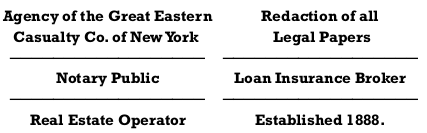
\includegraphics[keepaspectratio]{../img/Alfani.png}}

On the 27th of December, 1917, one Gallo, special investigator of the
state industrial commission, in company with one Geannelis, entered
defendant's office and he asked them what they wanted. Gallo stated that
he was selling his store, which consisted of a soda water stand,
together with a stock of cigars, cigarettes, etc., to Geannelis, for a
certain consideration, which was named, part of which was to be paid
down and the balance in installments. Gallo also stated there was a
certain amount due to the American Siphon Company on the purchase price
of the soda water fountain, which Geannelis was to assume and pay. The
defendant advised that Gallo give a bill of sale to Geannelis and that
he give a chattel mortgage for the amount remaining unpaid. He also
explained it would be necessary to file the mortgage in the county
clerk's office, so that the same could be foreclosed by the city marshal
in case of non-payment. His suggestions as to the bill of sale and
mortgage were followed and he thereupon prepared the same, for which he
was paid four dollars.

It is contended that this transaction, together with the sign, amounted
to a violation of the provisions of the statute quoted. I have been
unable to reach this conclusion. The statute, unless something is read
into it which does not there appear, is to prohibit a natural person
practicing or appearing as an attorney-at-law in the courts mentioned,
or to hold himself out to the public as being entitled to practice in
such courts. The defendant did neither. Clearly, the drafting of the
bill of sale and chattel mortgage was not practicing or appearing as an
attorney-at-law in any court. Nor did the words on the sign, ``Redaction
of all legal papers'' indicate that he was holding himself out as
entitled to practice in such courts. The words ``in any other manner,''
upon which stress is laid, relate to what precedes them in the sentence,
viz., the courts referred to. The phrase, although general in its
nature, is limited and qualified by the prior specific designations. The
rule of ejusdem generis applies. Where the enumeration of specific
things is followed by some more general word or phrase, such general
word or phrase is held to refer to the things of the same kind.

At the time defendant was convicted it was not illegal, and is not now,
for natural persons to draft papers usually intrusted to lawyers.
Judicial notice may be taken of the fact that in the rural districts of
the state leases, deeds, bills of sale, chattel mortgages, wills and
other instruments creating legal obligations are frequently prepared by
laymen, notaries public and justices of the peace. Indeed, a natural
person could, at the time defendant was convicted, appear for another in
a Magistrate's Court, or before a justice of the peace, except in cities
of the first and second class, and receive pay therefor. This practice
is recognized by section 271, which prohibits a person from receiving
compensation for appearing as attorney in a court before any magistrate
in any city of the first or second class, unless admitted to practice as
an attorney and counsellor in the courts of record of the state. That
the legislature did not intend to prohibit such practice is apparent
from the fact that at its last session it amended section 271, so that
it now includes cities of the third, as well as those of the first and
second class.

To give to the words ``in any other manner'' the legal effect suggested
would prohibit a natural person anywhere in the state from drawing a
legal paper of any description, or appearing in any court. This, the
legislature has not yet indicated its intent to do.

One of the well-settled rules of statutory construction is that
statutory offenses cannot be established by implication and that acts in
and of themselves innocent and lawful cannot be held to be criminal,
unless there is a clear and unequivocal expression of the legislative
intent to make them such.

I am of the opinion that the defendant was not guilty of violating
section 270 of the Penal Law; that the Appellate Division was right in
reversing the conviction and discharging him; and its judgment should,
therefore, be affirmed.

\subsection{Model Rules of Professional Conduct, Rule
5.5}\label{model-rules-of-professional-conduct-rule-5.5}

\subsubsection{Unauthorized Practice of Law; Multijurisdictional
Practiceof
Law}\label{unauthorized-practice-of-law-multijurisdictional-practiceof-law}

(a) A lawyer shall not practice law in a jurisdiction in violation of
the regulation of the legal profession in that jurisdiction, or assist
another in doing so.

(b) A lawyer who is not admitted to practice in this jurisdiction shall
not:

\begin{itemize}
\item
  (1) except as authorized by these Rules or other law, establish an
  office or other systematic and continuous presence in this
  jurisdiction for the practice of law; or
\item
  (2) hold out to the public or otherwise represent that the lawyer is
  admitted to practice law in this jurisdiction.
\end{itemize}

(c) A lawyer admitted in another United States jurisdiction, and not
disbarred or suspended from practice in any jurisdiction, may provide
legal services on a temporary basis in this jurisdiction that:

\begin{itemize}
\item
  (1) are undertaken in association with a lawyer who is admitted to
  practice in this jurisdiction and who actively participates in the
  matter;
\item
  (2) are in or reasonably related to a pending or potential proceeding
  before a tribunal in this or another jurisdiction, if the lawyer, or a
  person the lawyer is assisting, is authorized by law or order to
  appear in such proceeding or reasonably expects to be so authorized;
\item
  (3) are in or reasonably related to a pending or potential
  arbitration, mediation, or other alternative resolution proceeding in
  this or another jurisdiction, if the services arise out of or are
  reasonably related to the lawyer's practice in a jurisdiction in which
  the lawyer is admitted to practice and are not services for which the
  forum requires pro hac vice admission; or
\item
  (4) are not within paragraphs (c) (2) or (c)(3) and arise out of or
  are reasonably related to the lawyer's practice in a jurisdiction in
  which the lawyer is admitted to practice.
\end{itemize}

(d) A lawyer admitted in another United States jurisdiction or in a
foreign jurisdiction, and not disbarred or suspended from practice in
any jurisdiction or the equivalent thereof, or a person otherwise
lawfully practicing as an in-house counsel under the laws of a foreign
jurisdiction, may provide legal services through an office or other
systematic and continuous presence in this jurisdiction that:

\begin{itemize}
\item
  (1) are provided to the lawyer's employer or its organizational
  affiliates, are not services for which the forum requires pro hac vice
  admission; and when performed by a foreign lawyer and requires advice
  on the law of this or another U.S. jurisdiction or of the United
  States, such advice shall be based upon the advice of a lawyer who is
  duly licensed and authorized by the jurisdiction to provide such
  advice; or
\item
  (2) are services that the lawyer is authorized by federal or other law
  or rule to provide in this jurisdiction.
\end{itemize}

(e) For purposes of paragraph (d):

\begin{itemize}
\item
  (1) the foreign lawyer must be a member in good standing of a
  recognized legal profession in a foreign jurisdiction, the members of
  which are admitted to practice as lawyers or counselors at law or the
  equivalent, and subject to effective regulation and discipline by a
  duly constituted professional body or a public authority; or,
\item
  (2) the person otherwise lawfully practicing as an in-house counsel
  under the laws of a foreign jurisdiction must be authorized to
  practice under this Rule by, in the exercise of its discretion, {[}the
  highest court of this jurisdiction{]}.
\end{itemize}

\subsection{N.C. Gen.~Stat. § 84-2.1}\label{n.c.-gen.-stat.-84-2.1}

\subsubsection{``Practice law'' defined.}\label{practice-law-defined.}

(a) The phrase ``practice law'' as used in this Chapter is defined to be
performing any legal service for any other person, firm or corporation,
with or without compensation, specifically including the preparation or
aiding in the preparation of deeds, mortgages, wills, trust instruments,
inventories, accounts or reports of guardians, trustees, administrators
or executors, or preparing or aiding in the preparation of any petitions
or orders in any probate or court proceeding; abstracting or passing
upon titles, the preparation and filing of petitions for use in any
court, including administrative tribunals and other judicial or
quasi-judicial bodies, or assisting by advice, counsel, or otherwise in
any legal work; and to advise or give opinion upon the legal rights of
any person, firm or corporation: Provided, that the above reference to
particular acts which are specifically included within the definition of
the phrase ``practice law'' shall not be construed to limit the
foregoing general definition of the term, but shall be construed to
include the foregoing particular acts, as well as all other acts within
the general definition.

(b) The phrase ``practice law'' does not encompass:

\begin{itemize}
\item
  (1) The drafting or writing of memoranda of understanding or other
  mediation summaries by mediators at community mediation centers
  authorized by G.S.7A-38.5 or by mediators of employment-related
  matters for The University of North Carolina or a constituent
  institution, or for an agency, commission, or board of the State of
  North Carolina.
\item
  (2) The selection or completion of a preprinted form by a real estate
  broker licensed under Chapter 93A of the General Statutes, when the
  broker is acting as an agent in a real estate transaction and in
  accordance with rules adopted by the North Carolina Real Estate
  Commission, or the selection or completion of a preprinted residential
  lease agreement by any person or Web site provider. Nothing in this
  subdivision or in G.S.84-2.2 shall be construed to permit any person
  or Web site provider who is not licensed to practice law in accordance
  with this Chapter to prepare for any third person any contract or deed
  conveying any interest in real property, or to abstract or pass upon
  title to any real property, which is located in this State.
\item
  (3) The completion of or assisting a consumer in the completion of
  various agreements, contracts, forms, and other documents related to
  the sale or lease of a motor vehicle as defined in G.S.20-286(10), or
  of products or services ancillary or related to the sale or lease of a
  motor vehicle, by a motor vehicle dealer licensed under Article 12 of
  Chapter 20 of the General Statutes.
\end{itemize}

\subsection{Capital Associated Industries, Inc.~v. Stein, 922 F.3d 198
(4th Cir.
2019)}\label{capital-associated-industries-inc.-v.-stein-922-f.3d-198-4th-cir.-2019}

Capital Associated Industries, Inc.~(``CAI'') is a trade association
representing North Carolina employers. As part of a plan to expand its
membership, CAI wants to provide legal services to its members. But it
cannot because state law forbids corporations from practicing law.
Following unsuccessful lobbying efforts to change the law, CAI sued
state prosecutors to enjoin the enforcement of state unauthorized
practice of law (``UPL'') statutes against it. After the North Carolina
State Bar intervened to defend the statutes, the defendants obtained
summary judgment. On appeal, CAI contends that North Carolina's UPL
statutes violate its constitutional rights to free association, free
speech, and commercial speech; lack a rational basis; are void for
vagueness; and violate the state constitution. For the reasons that
follow, we affirm.

\subsubsection{I.}\label{i.}

\paragraph{A.}\label{a.}

Since 1931, the State of North Carolina has forbidden corporations from
practicing law. N.C. Gen Stat. § 84-5(a).\footnote{{[}n.1 in opinion{]}
  North Carolina is not alone in doing so. Almost all other states have
  similar laws on the books. One state allows unincorporated nonprofit
  ``associations'' to practice law. And CAI points to trade associations
  practicing law in a few other states. But at least one of those states
  bans corporations from practicing law.} To address the unauthorized
practice of law, the State Bar and state prosecutors may sue for an
injunction, and prosecutors may bring misdemeanor charges. The UPL
statutes do, however, allow the practice of law by lawyer-owned
professional corporations, public interest law firms, and in-house
counsel representing their employers.

CAI is a North Carolina nonprofit corporation that claims a tax
exemption under 26 U.S.C. § 501(c)(6) as a trade association of
employers. It has about 1,100 North Carolina employers as members and
describes its mission as fostering successful employment relationships.
CAI charges its members an annual fee adjusted for each member's size.
It competes with for-profit businesses in providing some services, such
as recruiting, background checks, consulting, training, conferences, and
affirmative action planning.

One of the most popular services it provides its members is a call
center, where members can speak to CAI's staff of human resources
experts. The experts can advise on HR issues. But they can't give legal
advice, even if they are licensed attorneys. So, when legal issues
arise, CAI's HR experts have to steer the conversation elsewhere, end
the conversation, or refer the member to outside counsel.

While it disclaims any interest in representing its members in court,
CAI would like to help them draft legal documents (such as contracts or
employee handbooks) and answer questions about employment and labor law.
If it could practice law, CAI would offer most legal services without
charge as part of its membership fees, but it would charge hourly fees
for certain services.

CAI has spent years trying to change the UPL statutes as part of its
``2X'' development plan to double its membership and reach. In 2011,
CAI's lobbyists persuaded state lawmakers to introduce bills that would
have allowed corporations to practice law. CAI tried and failed to get
the State Bar to support the bills. The State Bar instead actively
opposed the bills, and they were not enacted. CAI's lobbying efforts met
a similar fate in 2013. That same year, the State Bar adopted a proposed
ethics opinion advising that CAI would violate the UPL statutes if it
employed lawyers to give its members legal advice.

\paragraph{B.}\label{b.}

After two failed bids to achieve its goals through legislation, CAI
turned to the courts. It challenged the UPL statutes in federal district
court, naming as defendants the attorney general of North Carolina and
certain district attorneys. The complaint sought declaratory and
injunctive relief that would prevent enforcement of North Carolina's UPL
laws against it. It pleaded five claims under 42 U.S.C. § 1983
(concerning due process, free association, free speech, vagueness, and
commercial speech) and one claim under the state constitution.

The district court allowed the State Bar to intervene as a defendant. It
then denied CAI's motion for a preliminary injunction and the
defendants' motions to dismiss and for judgment on the pleadings. After
discovery, the parties cross-moved for summary judgment.

Before the district court, State Bar representatives expressed concerns
about nonlawyers controlling litigation and receiving attorney fees,
confidentiality, excessive fees, and the State Bar's inability to
discipline corporations. Regarding CAI, they worried about conflicts of
interest due to its large base of members and the fact that its
directors and officers don't have to be lawyers and thus wouldn't have
obligations under the State Bar's Rules of Professional Conduct.

To assuage these concerns, CAI filed declarations from three trade
organizations practicing law in other states, and it outlined a plan to
comply with ethics rules. CAI's lawyers would control legal services,
make decisions about conflicts of interest, and have sole access to
privileged communications. But CAI's directors and president would set
the attorneys' salaries and the legal department's budget. And CAI
declined to offer assurances that it would require its directors and
officers to be attorneys.

Some of CAI's members testified that allowing CAI to practice law would
mean that they could obtain more efficient and cost-effective legal
representation. But almost all those members said they had received
legal advice from private attorneys. Just one member said it had gone
without counsel in low-risk situations, but even it found counsel for
more serious matters. And according to CAI's President and CEO, no
member has left CAI because it doesn't offer legal services.

Addressing the cross-motions for summary judgment, the district court
first held that CAI had standing because it faced ``a credible threat of
prosecution'' if it practiced law. The district court then turned to the
merits and rejected all six of CAI's claims, entering summary judgment
for the defendants.

This appeal followed.

\subsubsection{III.}\label{iii.}

We begin with CAI's claim that the UPL statutes violate its freedom of
association. CAI contends that it is an expressive association seeking
to improve employment relationships in North Carolina and foster
compliance with the law. By forbidding it from practicing law, CAI
argues, the UPL statutes restrict its ability to carry out that
expressive mission. We agree with the district court, however, that the
UPL statutes do not unconstitutionally restrict CAI's associational
rights.

To support its argument, CAI relies on a line of cases beginning with
\emph{NAACP v. Button,} 371 U.S. 415, 83 S.Ct. 328, 9 L.Ed.2d 405
(1963). In \emph{Button,} the Supreme Court held that a Virginia law
forbidding organizations from retaining attorneys to represent third
parties infringed on the right of the NAACP and its members ``to
associate for the purpose of assisting persons who seek legal redress
for infringements'' of their civil and constitutional rights.

The Court emphasized that for the NAACP, litigation is ``not a technique
of resolving private differences; it is a means for achieving the lawful
objectives of equality of treatment.'' To win civil rights, the Court
said, litigation may be the ``sole practicable avenue'' and the ``most
effective form of political association.'' Thus, what was at stake was
``securing constitutionally guaranteed civil rights,'' not commercial
ends. And as the Court took time to emphasize, the law as applied
against the NAACP did not implicate ``professionally reprehensible
conflicts of interest.''

The Supreme Court has applied \emph{Button} in two contexts. The first,
involves public interest organizations like the NAACP. See \emph{In re
Primus}, 436 U.S. 412 (1978). In \emph{Primus,} the Court held that
South Carolina couldn't forbid the ACLU from advising people of their
legal rights and informing them that the ACLU could represent them for
free. The Court compared the ACLU's role to that of the NAACP in
\emph{Button} and contrasted it with ``a group that exists for the
primary purpose of financial gain.'' It cast doubt on whether an
organization operating for financial gain would receive the same
protection as organizations that promote the common political aims of
their members.

The second context involves labor unions. \emph{See} \emph{Bhd. of R.R.
Trainmen v. Va. ex rel. Va. State Bar,} 377 U.S. 1 (1964). The
\emph{Trainmen} Court held that Virginia couldn't bar a union from
recommending lawyers to its members for workers' compensation suits. The
Virginia law, the Court said, infringed on ``the right of individuals
and the public to be fairly represented in lawsuits authorized by
Congress to effectuate a basic public interest'' without adequate
justification.

The Court has extended \emph{Trainmen} twice. First, it held that
Illinois couldn't prevent a union from employing attorneys to represent
its members in workers' compensation claims. \emph{United Mine Workers
v. Ill. State Bar Ass'n,} 389 U.S. 217 (1967). While the Court
considered that law unjustified, it emphasized that the state did
possess an ``interest in high standards of legal ethics.'' Second, the
Court held that Michigan couldn't bar a union from recommending to its
members certain attorneys who had agreed to a maximum fee. \emph{United
Transp. Union v. State Bar of Mich.,} 401 U.S. 576 (1971). ``At issue,''
the Court said, ``is the basic right to group legal action'' and the
right to ``meaningful access to the courts,'' which required enabling
union members to ``meet the costs of legal representation.''

The ``common thread running through'' these cases is that ``collective
activity undertaken to obtain meaningful access to the courts is a
fundamental right.'' Critically, however, the cases distinguish between
the commercial practice of law and ``associating for non-commercial
purposes to advocate the enforcement of legal and constitutional
rights.''

The Supreme Court emphasized this distinction in \emph{Ohralik v. Ohio
State Bar Ass'n}, 436 U.S. 447 (1978). In \emph{Ohralik}, the Court
rejected a challenge to an Ohio law forbidding in-person solicitation of
clients. Solicitation of clients for commercial purposes, the Court
held, did not implicate ``political expression or an exercise of
associational freedom'' or ``mutual assistance in asserting legal
rights.''

As applied to CAI, North Carolina's UPL laws are closer to the statute
in \emph{Ohralik} than the statutes in the \emph{Button} cases. While
this case is admittedly close, several considerations distinguish CAI's
proposed practice from the \emph{Button} line of cases. First, what CAI
seeks to accomplish would be for commercial ends and would address only
private concerns. Second, it would not facilitate access to the courts.
And third, it would pose ethical concerns not present in the
\emph{Button} cases.

When organizations like the NAACP and the ACLU solicit clients and
retain lawyers to represent them, they express their commitment to
expanding and guarding civil rights. CAI, in contrast, wants to help its
members ``resolve private differences'' by drafting legal documents and
advising employers on labor and employment issues. Its goal, as set
forth in its 2X plan, is to increase revenues and recruit new members
who will pay dues and additional legal fees. CAI would charge by the
hour for some services. While other services would be included in its
membership fees, CAI's chairman said the trade association might
increase its fees if it could practice law. CAI thus seeks to practice
law for commercial ends, like a private attorney---not to associate for
political or otherwise public goals. And while we accept that CAI
engages in some expressive activity, CAI proposes to practice law for
commercial ends, not to express a message.

Nor does CAI propose to engage in ``collective activity undertaken to
obtain meaningful access to the courts.'' As described in the record,
CAI's members have consistently had access to legal services and the
courts. And CAI has no intention of litigating in any forum. So, unlike
the organizations in the \emph{Button} cases, CAI would not facilitate
access to justice or vindicate its members' constitutional or statutory
rights. CAI's proposed practice might reduce some of its members' legal
bills. But nothing in the record shows that CAI's inability to practice
law means that its members can't ``meet the costs of legal
representation'' or obtain ``meaningful access to the courts.''

The Supreme Court has, moreover, extended associational rights only when
the proposed practice of law wouldn't raise ethical concerns. CAI's
proposed practice, in contrast, does raise ethical concerns.
Specifically, its members would pay legal fees for representation by
attorneys supervised by officers and directors who are not attorneys.
That structure (even if housed in a nonprofit entity) could compromise
the independence and professional judgment of the lawyers involved, and
the corporation's interests could trump loyalty to clients.

In sum, several features of CAI's proposed practice distinguish it from
the organizations in the \emph{Button} cases. As a result, like the
solicitation statute in \emph{Ohralik,} North Carolina's UPL statutes
``only marginally affect \ldots{} First Amendment concerns.'' Because
they do not ``substantially impair the associational rights'' of CAI, we
need not examine whether the state's interests suffice to justify them.
We hold that the UPL statutes do not violate CAI's associational rights.

\subsubsection{IV.}\label{iv.}

Next, CAI argues that the UPL statutes unlawfully burden its freedom of
speech. The district court rejected this claim based on the so-called
``professional speech doctrine.'' When the district court ruled, this
circuit and others applied lesser standards of scrutiny to
professionals' speech to clients. But after the briefing in this appeal,
the Supreme Court disapproved of this doctrine. \emph{See} \emph{Nat'l
Inst. of Family \& Life Advocates v. Becerra (NIFLA)}, 138 S.Ct. 2361
(2018).

In \emph{NIFLA,} the Court addressed a California law requiring certain
clinics that primarily serve pregnant women to post notices about what
services they didn't offer and about free state services. Although the
law applied in a professional context, the Court approached the case as
it would any other involving compelled speech. It held that the law was
content-based. And because it held that the law could not survive
intermediate scrutiny, the Court declined to decide whether strict
scrutiny should apply.

The Court did, however, recognize two situations in which states have
broader authority to regulate the speech of professionals than that of
nonprofessionals. First, there is ``more deferential review'' for
requirements that professionals ``disclose factual, noncontroversial
information'' in their commercial speech. Second, ``states may regulate
professional conduct, even though that conduct incidentally involves
speech.'' As examples of this latter category, the Court cited cases
about malpractice, anticompetitive agreements, client solicitation, and
informed consent.

On appeal, North Carolina describes the ban on corporate law practice as
a regulation of professional conduct that incidentally burdens speech,
which only needs to survive intermediate scrutiny. In contrast, CAI
describes it as a content-based and identity-based regulation of speech
that must survive strict scrutiny. As explained below, we agree with the
state that the law passes---and only needs to pass---intermediate
scrutiny.

\paragraph{A.}\label{a.-1}

North Carolina's ban on the practice of law by corporations fits within
\emph{NIFLA}'s exception for professional regulations that incidentally
affect speech. The ban is part of a generally applicable licensing
regime that restricts the practice of law to bar members and entities
owned by bar members. In this case, any impact the UPL statutes have on
speech is incidental to the overarching purpose of regulating who may
practice law.

Many laws that regulate the conduct of a profession or business place
incidental burdens on speech, yet the Supreme Court has treated them
differently than restrictions on speech. Bans on discrimination, price
regulations, and laws against anticompetitive activities all implicate
speech---some may implicate speech even more directly than licensing
requirements. But the Supreme Court has analyzed them all as regulations
of conduct.

As CAI recognizes, the practice of law has communicative and
non-communicative aspects. The UPL statutes don't target the
communicative aspects of practicing law, such as the advice lawyers may
give to clients. Instead, they focus more broadly on the question of who
may conduct themselves as a lawyer. Licensing laws inevitably have some
effect on the speech of those who are not (or cannot be) licensed. But
that effect is merely incidental to the primary objective of regulating
the conduct of the profession.

\paragraph{B.}\label{b.-1}

Having determined that the UPL statutes regulate conduct, we turn to the
appropriate standard of review. CAI urges us to apply strict scrutiny,
contending that the UPL statutes restrict speech based on the content
and on the speaker. We think the correct reading of Supreme Court
precedent, however, is that intermediate scrutiny should apply to
regulations of conduct that incidentally impact speech.

\paragraph{C.}\label{c.}

We turn then to consider whether North Carolina's ban on the practice of
law survives this standard of review. To survive intermediate scrutiny,
the defendant must show ``a substantial state interest'' and a solution
that is ``sufficiently drawn'' to protect that interest. North
Carolina's interest in regulating the legal profession to protect
clients is at least substantial. In fact, the Supreme Court has
repeatedly described that interest in even stronger terms.

Barring corporations from practicing law is sufficiently drawn to
protect that interest. Professional integrity could suffer if the state
allows lawyers to practice on behalf of organizations owned and run by
nonlawyers and to collect legal fees from clients. Nonlawyers would
likely supervise lawyers representing third-party clients at CAI, which
could compromise professional judgment and generate conflicts between
client interests and the corporation's interests.

The state has addressed these problems by proscribing law practice by
organizations that pose the most danger, while exempting organizations
that pose little danger. Professional corporations, for example, must be
owned exclusively by lawyers. N.C. Gen.~Stat. § 55B-4(2). And public
interest law firms ``must have a governing structure that does not
permit'' anyone except an ``attorney duly licensed\ldots{} to control
the manner or course of the legal services rendered.'' Plus, the
restrictions on the fees such firms may receive makes it impossible for
them break even (much less turn a profit) on legal work.

Another state legislature might balance the interests differently. But
intermediate scrutiny requires only a ``reasonable fit between the
challenged regulation'' and the state's interest---not the least
restrictive means. Because North Carolina has established a reasonable
fit between its UPL statutes and a substantial government interest, the
UPL statutes survive intermediate scrutiny.

\subsubsection{V.}\label{v.}

CAI also argues that the UPL statutes deny it due process because they
lack a rational basis. CAI doesn't contend that its due process claim
concerns fundamental rights, so the UPL statutes are only subject to
rational basis review. To pass muster under rational basis review,
legislation ``need only be rationally related to a legitimate government
interest.''

The state relies on the same justifications it provided in response to
the First Amendment claims. As our precedent counsels, ``there is a
rational basis to restrict corporate \ldots{} ownership of professional
businesses'' to protect consumers. Accordingly, we agree with the
district court that the state's justifications suffice. CAI's remaining
arguments---such as the availability of less restrictive means---are
inapposite for rational basis review. We hold that the UPL statutes do
not deny CAI due process.

\subsubsection{VI.}\label{vi.}

CAI also contends that the UPL statutes are unconstitutionally vague
because they fail to provide fair notice of what it means to practice
law. A statute is unconstitutionally vague if it ``fails to provide a
person of ordinary intelligence fair notice of what is prohibited, or is
so standardless that it authorizes or encourages seriously
discriminatory enforcement.'' But ``perfect clarity and precise guidance
have never been required even of regulations that restrict expressive
activity.''

To determine if a statute is vague, we examine both the statute itself
and any limiting constructions from state courts or agencies. State law
defines the term ``practice law'' as ``performing any legal service.''
N.C. Gen.~Stat. § 84-2.1(a). The statutory definition provides a lengthy
but unexhaustive list of what does and doesn't count as a legal service.
The statute prohibiting the unauthorized practice of law elaborates on
the definition further. And North Carolina courts have expounded on this
definition at length.

CAI's vagueness challenge fails. The statutes and state case law
collectively provide an extensive definition of what it means to
practice law. Between them, a person of ordinary intelligence would have
fair notice of what the UPL statutes prohibit. Indeed, CAI itself
understood what it means to practice law well enough to avoid giving its
members legal advice.

CAI points out that State Bar officials couldn't present a clear answer
to every hypothetical question asked in their depositions. But fair
notice doesn't require certainty about every hypothetical situation. We
hold, therefore, that the UPL statutes are not void for vagueness.

\subsubsection{VII.}\label{vii.}

CAI next contends that the UPL statutes violate the state constitution's
Monopoly Clause, which provides that ``perpetuities and monopolies
\ldots{} shall not be allowed.''

The Supreme Court of North Carolina has interpreted this clause to allow
``reasonable regulations'' of commerce with a substantial relationship
to public health, safety, or welfare. That court has long been
deferential toward professional regulations, regularly upholding
professional licensing requirements.

The state high court has twice upheld the ban on corporate law practice.
In \emph{Seawell,} the Supreme Court of North Carolina affirmed an
injunction against a corporation for the unauthorized practice of law,
holding that ``the statute in question offends neither the State nor
Federal Constitution.'' And in \emph{Gardner v. North Carolina State
Bar,} that court held that an insurance company could not employ an
attorney to represent its insureds, finding that ``there is no merit to
the argument'' that the ban on corporate practice ``violates Article I
of the state constitution and the Fourteenth Amendment.'' Although it is
unclear whether \emph{Seawell} and \emph{Gardner} addressed Monopoly
Clause arguments, they illustrate the leeway North Carolina courts give
the legislature to regulate the legal profession.

It is well established that the practice of law affects the public
interest and that the unregulated practice of law can pose a danger.
Based on the applicable state case law, this court must conclude that
the UPL statutes do not violate the Monopoly Clause.

\subsubsection{VIII.}\label{viii.}

Last, CAI argues that it has a free speech right to advertise the legal
services it wants to offer. But this commercial speech claim is not an
independent basis for granting relief, and the state may forbid CAI from
advertising legal services barred by law.

\emph{AFFIRMED.}

\subsection{Note: Challenge to North Carolina Unauthorized Practice
Statute}\label{note-challenge-to-north-carolina-unauthorized-practice-statute}

A pending suit, brought by ``two North Carolina Certified Paralegals and
the \href{https://www.ncjfap.org/}{North Carolina Justice for All
Project}, a nonprofit organization founded \ldots{} to expand access to
justice in North Carolina'', challenges the constitutionality of the
North Carolina unauthorized practice statute ``as applied to pure legal
advice.'' \emph{Black Polaski v. Lee}, No.~7-24-cv-00004-BO-BM
(E.D.N.C.). Review the
\href{../exhibits/BlackPolaskiComplaint.pdf}{complaint in \emph{Black
Polaski}} and consider whether the claims may be distinguishable from
those in \emph{Capital Associated Industries}.

\section{Law Firms}\label{law-firms}

\subsection{Model Rules of Professional Conduct, Rule
5.1}\label{model-rules-of-professional-conduct-rule-5.1}

\subsubsection{Responsibilities of a Partner or Supervisory
Lawyer}\label{responsibilities-of-a-partner-or-supervisory-lawyer}

(a) A partner in a law firm, and a lawyer who individually or together
with other lawyers possesses comparable managerial authority in a law
firm, shall make reasonable efforts to ensure that the firm has in
effect measures giving reasonable assurance that all lawyers in the firm
conform to the Rules of Professional Conduct.

(b) A lawyer having direct supervisory authority over another lawyer
shall make reasonable efforts to ensure that the other lawyer conforms
to the Rules of Professional Conduct.

(c) A lawyer shall be responsible for another lawyer's violation of the
Rules of Professional Conduct if:

\begin{itemize}
\item
  (1) the lawyer orders or, with knowledge of the specific conduct,
  ratifies the conduct involved; or
\item
  (2) the lawyer is a partner or has comparable managerial authority in
  the law firm in which the other lawyer practices, or has direct
  supervisory authority over the other lawyer, and knows of the conduct
  at a time when its consequences can be avoided or mitigated but fails
  to take reasonable remedial action.
\end{itemize}

\subsection{Model Rules of Professional Conduct, Rule
5.2}\label{model-rules-of-professional-conduct-rule-5.2}

\subsubsection{Responsibilities of a Subordinate
Lawyer}\label{responsibilities-of-a-subordinate-lawyer}

(a) A lawyer is bound by the Rules of Professional Conduct
notwithstanding that the lawyer acted at the direction of another
person.

(b) A subordinate lawyer does not violate the Rules of Professional
Conduct if that lawyer acts in accordance with a supervisory lawyer's
reasonable resolution of an arguable question of professional duty.

\subsection{Model Rules of Professional Conduct, Rule
5.3}\label{model-rules-of-professional-conduct-rule-5.3}

\subsubsection{Responsibilities Regarding Nonlawyer
Assistance}\label{responsibilities-regarding-nonlawyer-assistance}

With respect to a nonlawyer employed or retained by or associated with a
lawyer:

(a) a partner, and a lawyer who individually or together with other
lawyers possesses comparable managerial authority in a law firm shall
make reasonable efforts to ensure that the firm has in effect measures
giving reasonable assurance that the person's conduct is compatible with
the professional obligations of the lawyer;

(b) a lawyer having direct supervisory authority over the nonlawyer
shall make reasonable efforts to ensure that the person's conduct is
compatible with the professional obligations of the lawyer; and

(c) a lawyer shall be responsible for conduct of such a person that
would be a violation of the Rules of Professional Conduct if engaged in
by a lawyer if:

\begin{itemize}
\item
  (1) the lawyer orders or, with the knowledge of the specific conduct,
  ratifies the conduct involved; or
\item
  (2) the lawyer is a partner or has comparable managerial authority in
  the law firm in which the person is employed, or has direct
  supervisory authority over the person, and knows of the conduct at a
  time when its consequences can be avoided or mitigated but fails to
  take reasonable remedial action.
\end{itemize}

\subsection{Model Rules of Professional Conduct, Rule
5.4}\label{model-rules-of-professional-conduct-rule-5.4}

\subsubsection{Professional Independence of a
Lawyer}\label{professional-independence-of-a-lawyer}

(a) A lawyer or law firm shall not share legal fees with a nonlawyer,
except that:

\begin{itemize}
\item
  (1) an agreement by a lawyer with the lawyer's firm, partner, or
  associate may provide for the payment of money, over a reasonable
  period of time after the lawyer's death, to the lawyer's estate or to
  one or more specified persons;
\item
  (2) a lawyer who purchases the practice of a deceased, disabled, or
  disappeared lawyer may, pursuant to the provisions of Rule 1.17, pay
  to the estate or other representative of that lawyer the agreed-upon
  purchase price;
\item
  (3) a lawyer or law firm may include nonlawyer employees in a
  compensation or retirement plan, even though the plan is based in
  whole or in part on a profit-sharing arrangement; and
\item
  (4) a lawyer may share court-awarded legal fees with a nonprofit
  organization that employed, retained or recommended employment of the
  lawyer in the matter.
\end{itemize}

(b) A lawyer shall not form a partnership with a nonlawyer if any of the
activities of the partnership consist of the practice of law.

(c) A lawyer shall not permit a person who recommends, employs, or pays
the lawyer to render legal services for another to direct or regulate
the lawyer's professional judgment in rendering such legal services.

(d) A lawyer shall not practice with or in the form of a professional
corporation or association authorized to practice law for a profit, if:

\begin{itemize}
\item
  (1) a nonlawyer owns any interest therein, except that a fiduciary
  representative of the estate of a lawyer may hold the stock or
  interest of the lawyer for a reasonable time during administration;
\item
  (2) a nonlawyer is a corporate director or officer thereof or occupies
  the position of similar responsibility in any form of association
  other than a corporation ; or
\item
  (3) a nonlawyer has the right to direct or control the professional
  judgment of a lawyer.
\end{itemize}

\subsection{Model Rules of Professional Conduct, Rule
5.6}\label{model-rules-of-professional-conduct-rule-5.6}

\subsubsection{Restrictions on Rights to
Practice}\label{restrictions-on-rights-to-practice}

A lawyer shall not participate in offering or making:

(a) a partnership, shareholders, operating, employment, or other similar
type of agreement that restricts the right of a lawyer to practice after
termination of the relationship, except an agreement concerning benefits
upon retirement; or

(b) an agreement in which a restriction on the lawyer's right to
practice is part of the settlement of a client controversy.

\subsection{Model Rules of Professional Conduct, Rule
5.7}\label{model-rules-of-professional-conduct-rule-5.7}

\subsubsection{Responsibilities Regarding Law-related
Services}\label{responsibilities-regarding-law-related-services}

(a) A lawyer shall be subject to the Rules of Professional Conduct with
respect to the provision of law-related services, as defined in
paragraph (b), if the law-related services are provided:

\begin{itemize}
\item
  (1) by the lawyer in circumstances that are not distinct from the
  lawyer's provision of legal services to clients; or
\item
  (2) in other circumstances by an entity controlled by the lawyer
  individually or with others if the lawyer fails to take reasonable
  measures to assure that a person obtaining the law-related services
  knows that the services are not legal services and that the
  protections of the client-lawyer relationship do not exist.
\end{itemize}

(b) The term ``law-related services'' denotes services that might
reasonably be performed in conjunction with and in substance are related
to the provision of legal services, and that are not prohibited as
unauthorized practice of law when provided by a nonlawyer.

\chapter{Advertising \& Solicitation}\label{advertising-solicitation}

\section{Advertising}\label{advertising}

\subsection{Model Rules of Professional Conduct, Rule
7.1}\label{model-rules-of-professional-conduct-rule-7.1}

\subsubsection{Communications Concerning a Lawyer's
Services}\label{communications-concerning-a-lawyers-services}

A lawyer shall not make a false or misleading communication about the
lawyer or the lawyer's services. A communication is false or misleading
if it contains a material misrepresentation of fact or law, or omits a
fact necessary to make the statement considered as a whole not
materially misleading.

\subsection{Model Rules of Professional Conduct, Rule
7.2}\label{model-rules-of-professional-conduct-rule-7.2}

\subsubsection{Communications Concerning a Lawyer's Services: Specific
Rules}\label{communications-concerning-a-lawyers-services-specific-rules}

(a) A lawyer may communicate information regarding the lawyer's services
through any media.

(b) A lawyer shall not compensate, give or promise anything of value to
a person for recommending the lawyer's services except that a lawyer
may:

\begin{itemize}
\item
  (1) pay the reasonable costs of advertisements or communications
  permitted by this Rule;
\item
  (2) pay the usual charges of a legal service plan or a not-for-profit
  or qualified lawyer referral service;
\item
  (3) pay for a law practice in accordance with Rule 1.17;
\item
  (4) refer clients to another lawyer or a nonlawyer professional
  pursuant to an agreement not otherwise prohibited under these Rules
  that provides for the other person to refer clients or customers to
  the lawyer, if:

  \begin{itemize}
  \item
    (i) the reciprocal referral agreement is not exclusive; and
  \item
    (ii) the client is informed of the existence and nature of the
    agreement; and
  \end{itemize}
\item
  (5) give nominal gifts as an expression of appreciation that are
  neither intended nor reasonably expected to be a form of compensation
  for recommending a lawyer's services.
\end{itemize}

(c) A lawyer shall not state or imply that a lawyer is certified as a
specialist in a particular field of law, unless:

\begin{itemize}
\item
  (1) the lawyer has been certified as a specialist by an organization
  that has been approved by an appropriate authority of the state or the
  District of Columbia or a U.S. Territory or that has been accredited
  by the American Bar Association; and
\item
  (2) the name of the certifying organization is clearly identified in
  the communication.
\end{itemize}

(d) Any communication made under this Rule must include the name and
contact information of at least one lawyer or law firm responsible for
its content.

\subsection{Bates v. State Bar of Arizona, 433 U.S. 350
(1977)}\label{bates-v.-state-bar-of-arizona-433-u.s.-350-1977}

\subsubsection{MR. JUSTICE BLACKMUN delivered the opinion of the
Court.}\label{mr.-justice-blackmun-delivered-the-opinion-of-the-court.}

As part of its regulation of the Arizona Bar, the Supreme Court of that
State has imposed and enforces a disciplinary rule that restricts
advertising by attorneys. This case presents two issues: whether §§ 1
and 2 of the Sherman Act, 15 U. S. C. §§ 1 and 2, forbid such state
regulation, and whether the operation of the rule violates the First
Amendment, made applicable to the States through the Fourteenth.

\subsubsection{I}\label{i}

Appellants John R. Bates and Van O'Steen are attorneys licensed to
practice law in the State of Arizona. As such, they are members of the
appellee, the State Bar of Arizona. After admission to the bar in 1972,
appellants worked as attorneys with the Maricopa County Legal Aid
Society.

In March 1974, appellants left the Society and opened a law office,
which they call a ``legal clinic,'' in Phoenix. Their aim was to provide
legal services at modest fees to persons of moderate income who did not
qualify for governmental legal aid. In order to achieve this end, they
would accept only routine matters, such as uncontested divorces,
uncontested adoptions, simple personal bankruptcies, and changes of
name, for which costs could be kept down by extensive use of paralegals,
automatic typewriting equipment, and standardized forms and office
procedures. More complicated cases, such as contested divorces, would
not be accepted. Because appellants set their prices so as to have a
relatively low return on each case they handled, they depended on
substantial volume.

After
{\marginnote{\begin{footnotesize}\pandocbounded{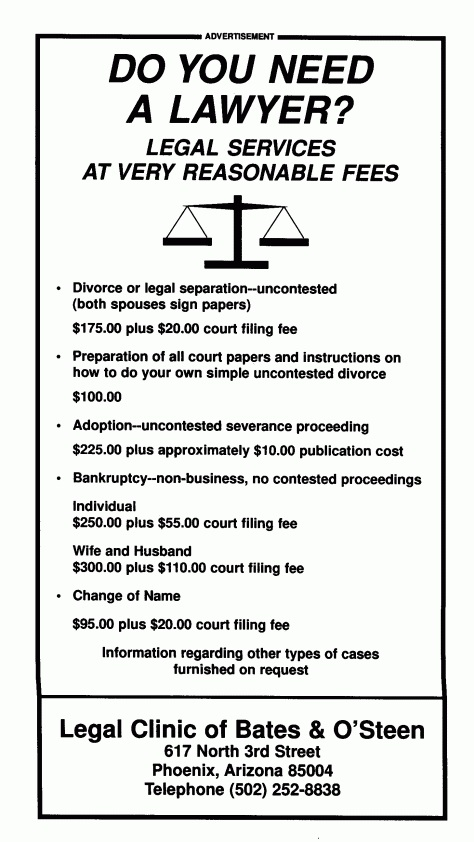
\includegraphics[keepaspectratio]{../img/bates.jpg}}\end{footnotesize}}}
conducting their practice in this manner for two years, appellants
concluded that their practice and clinical concept could not survive
unless the availability of legal services at low cost was advertised
and, in particular, fees were advertised. Consequently, in order to
generate the necessary flow of business, that is, ``to attract
clients,'' appellants on February 22, 1976, placed an advertisement in
the Arizona Republic, a daily newspaper of general circulation in the
Phoenix metropolitan area. As may be seen, the advertisement stated that
appellants were offering ``legal services at very reasonable fees,'' and
listed their fees for certain services.

Appellants concede that the advertisement constituted a clear violation
of Disciplinary Rule 2-101(B). The disciplinary rule provides in part:

\begin{quote}
(B) A lawyer shall not publicize himself, or his partner, or associate,
or any other lawyer affiliated with him or his firm, as a lawyer through
newspaper or magazine advertisements, radio or television announcements,
display advertisements in the city or telephone directories or other
means of commercial publicity, nor shall he authorize or permit others
to do so in his behalf.
\end{quote}

Upon the filing of a complaint initiated by the president of the State
Bar, a hearing was held before a three member Special Local
Administrative Committee. Although the committee took the position that
it could not consider an attack on the validity of the rule, it allowed
the parties to develop a record on which such a challenge could be
based. The committee recommended that each of the appellants be
suspended from the practice of law for not less than six months. Upon
further review by the Board of Governors of the State Bar, the Board
recommended only a one-week suspension for each appellant, the weeks to
run consecutively.

Appellants then sought review in the Supreme Court of Arizona, arguing,
among other things, that the disciplinary rule violated §§ 1 and 2 of
the Sherman Act because of its tendency to limit competition, and that
the rule infringed their First Amendment rights. The court rejected both
claims. The plurality may have viewed with some skepticism the claim
that a restraint on advertising might have an adverse effect on
competition. But, even if the rule might otherwise violate the Act, the
plurality concluded that the regulation was exempt from Sherman Act
attack because the rule ``is an activity of the State of Arizona acting
as sovereign.'' The regulation thus was held to be shielded from the
Sherman Act by the state-action exemption.

Turning to the First Amendment issue, the plurality noted that
restrictions on professional advertising have survived constitutional
challenge in the past. Although recognizing that \emph{Virginia Pharmacy
Board v. Virginia Consumer Council} and \emph{Bigelow v. Virginia} held
that commercial speech was entitled to certain protection under the
First Amendment, the plurality focused on passages in those opinions
acknowledging that special considerations might bear on the advertising
of professional services by lawyers. The plurality apparently was of the
view that the older decisions dealing with professional advertising
survived these recent cases unscathed, and held that Disciplinary Rule
2-101(B) passed First Amendment muster. Because the court, in agreement
with the Board of Governors, felt that appellants' advertising ``was
done in good faith to test the constitutionality of DR 2-101(B),'' it
reduced the sanction to censure only.

Of particular interest here is the opinion of Mr.~Justice Holohan in
dissent. In his view, the case should have been framed in terms of ``the
right of the public as consumers and citizens to know about the
activities of the legal profession,'' rather than as one involving
merely the regulation of a profession. Observed in this light, he felt
that the rule performed a substantial disservice to the public:

\begin{quote}
Obviously the information of what lawyers charge is important for
private economic decisions by those in need of legal services. Such
information is also helpful, perhaps indispensable, to the formation of
an intelligent opinion by the public on how well the legal system is
working and whether it should be regulated or even altered. The rule at
issue prevents access to such information by the public.
\end{quote}

Although the dissenter acknowledged that some types of advertising might
cause confusion and deception, he felt that the remedy was to ban that
form, rather than all advertising. Thus, despite his ``personal dislike
of the concept of advertising by attorneys,'' he found the ban
unconstitutional.

\subsubsection{III. The First Amendment}\label{iii.-the-first-amendment}

The issue presently before us is a narrow one. First, we need not
address the peculiar problems associated with advertising claims
relating to the quality of legal services. Such claims probably are not
susceptible of precise measurement or verification and, under some
circumstances, might well be deceptive or misleading to the public, or
even false. Appellee does not suggest, nor do we perceive, that
appellants' advertisement contained claims, extravagant or otherwise, as
to the quality of services. Accordingly, we leave that issue for another
day. Second, we also need not resolve the problems associated with
in-person solicitation of clients---at the hospital room or the accident
site, or in any other situation that breeds undue influence---by
attorneys or their agents or ``runners.'' Activity of that kind might
well pose dangers of overreaching and misrepresentation not encountered
in newspaper announcement advertising. Hence, this issue also is not
before us. Third, we note that appellee's criticism of advertising by
attorneys does not apply with much force to some of the basic factual
content of advertising: information as to the attorney's name, address,
and telephone number, office hours, and the like. The American Bar
Association itself has a provision in its current Code of Professional
Responsibility that would allow the disclosure of such information, and
more, in the classified section of the telephone directory. We
recognize, however, that an advertising diet limited to such spartan
fare would provide scant nourishment.

The heart of the dispute before us today is whether lawyers also may
constitutionally advertise the prices at which certain routine services
will be performed. Numerous justifications are proffered for the
restriction of such price advertising. We consider each in turn:

1. The Adverse Effect on Professionalism. Appellee places particular
emphasis on the adverse effects that it feels price advertising will
have on the legal profession. The key to professionalism, it is argued,
is the sense of pride that involvement in the discipline generates. It
is claimed that price advertising will bring about commercialization,
which will undermine the attorney's sense of dignity and self-worth. The
hustle of the marketplace will adversely affect the profession's service
orientation, and irreparably damage the delicate balance between the
lawyer's need to earn and his obligation selflessly to serve.
Advertising is also said to erode the client's trust in his attorney:
Once the client perceives that the lawyer is motivated by profit, his
confidence that the attorney is acting out of a commitment to the
client's welfare is jeopardized. And advertising is said to tarnish the
dignified public image of the profession.

We recognize, of course, and commend the spirit of public service with
which the profession of law is practiced and to which it is dedicated.
The present Members of this Court, licensed attorneys all, could not
feel otherwise. And we would have reason to pause if we felt that our
decision today would undercut that spirit. But we find the postulated
connection between advertising and the erosion of true professionalism
to be severely strained. At its core, the argument presumes that
attorneys must conceal from themselves and from their clients the
real-life fact that lawyers earn their livelihood at the bar. We suspect
that few attorneys engage in such self-deception. And rare is the
client, moreover, even one of modest means, who enlists the aid of an
attorney with the expectation that his services will be rendered free of
charge. In fact, the American Bar Association advises that an attorney
should reach ``a clear agreement with his client as to the basis of the
fee charges to be made,'' and that this is to be done ``as soon as
feasible after a lawyer has been employed.'' If the commercial basis of
the relationship is to be promptly disclosed on ethical grounds, once
the client is in the office, it seems inconsistent to condemn the candid
revelation of the same information before he arrives at that office.

Moreover, the assertion that advertising will diminish the attorney's
reputation in the community is open to question. Bankers and engineers
advertise, and yet these professions are not regarded as undignified. In
fact, it has been suggested that the failure of lawyers to advertise
creates public disillusionment with the profession. The absence of
advertising may be seen to reflect the profession's failure to reach out
and serve the community: Studies reveal that many persons do not obtain
counsel even when they perceive a need because of the feared price of
services or because of an inability to locate a competent attorney.
Indeed, cynicism with regard to the profession may be created by the
fact that it long has publicly eschewed advertising, while condoning the
actions of the attorney who structures his social or civic associations
so as to provide contacts with potential clients.

It appears that the ban on advertising originated as a rule of etiquette
and not as a rule of ethics. Early lawyers in Great Britain viewed the
law as a form of public service, rather than as a means of earning a
living, and they looked down on ``trade'' as unseemly. Eventually, the
attitude toward advertising fostered by this view evolved into an aspect
of the ethics of the profession. But habit and tradition are not in
themselves an adequate answer to a constitutional challenge. In this
day, we do not belittle the person who earns his living by the strength
of his arm or the force of his mind. Since the belief that lawyers are
somehow ``above'' trade has become an anachronism, the historical
foundation for the advertising restraint has crumbled.

2. The Inherently Misleading Nature of Attorney Advertising. It is
argued that advertising of legal services inevitably will be misleading
(a) because such services are so individualized with regard to content
and quality as to prevent informed comparison on the basis of an
advertisement, (b) because the consumer of legal services is unable to
determine in advance just what services he needs, and (c) because
advertising by attorneys will highlight irrelevant factors and fail to
show the relevant factor of skill.

We are not persuaded that restrained professional advertising by lawyers
inevitably will be misleading. Although many services performed by
attorneys are indeed unique, it is doubtful that any attorney would or
could advertise fixed prices for services of that type. The only
services that lend themselves to advertising are the routine ones: the
uncontested divorce, the simple adoption, the uncontested personal
bankruptcy, the change of name, and the like---the very services
advertised by appellants. Although the precise service demanded in each
task may vary slightly, and although legal services are not fungible,
these facts do not make advertising misleading so long as the attorney
does the necessary work at the advertised price. The argument that legal
services are so unique that fixed rates cannot meaningfully be
established is refuted by the record in this case: The appellee State
Bar itself sponsors a Legal Services Program in which the participating
attorneys agree to perform services like those advertised by the
appellants at standardized rates. Indeed, until the decision of this
Court in \emph{Goldfarb v. Virginia State Bar}, the Maricopa County Bar
Association apparently had a schedule of suggested minimum fees for
standard legal tasks. We thus find of little force the assertion that
advertising is misleading because of an inherent lack of standardization
in legal services.

The second component of the argument---that advertising ignores the
diagnostic role---fares little better. It is unlikely that many people
go to an attorney merely to ascertain if they have a clean bill of legal
health. Rather, attorneys are likely to be employed to perform specific
tasks. Although the client may not know the detail involved in
performing the task, he no doubt is able to identify the service he
desires at the level of generality to which advertising lends itself.

The third component is not without merit: Advertising does not provide a
complete foundation on which to select an attorney. But it seems
peculiar to deny the consumer, on the ground that the information is
incomplete, at least some of the relevant information needed to reach an
informed decision. The alternative---the prohibition of
advertising---serves only to restrict the information that flows to
consumers. Moreover, the argument assumes that the public is not
sophisticated enough to realize the limitations of advertising, and that
the public is better kept in ignorance than trusted with correct but
incomplete information. We suspect the argument rests on an
underestimation of the public. In any event, we view as dubious any
justification that is based on the benefits of public ignorance.
Although, of course, the bar retains the power to correct omissions that
have the effect of presenting an inaccurate picture, the preferred
remedy is more disclosure, rather than less. If the naiveté of the
public will cause advertising by attorneys to be misleading, then it is
the bar's role to assure that the populace is sufficiently informed as
to enable it to place advertising in its proper perspective.

3. The Adverse Effect on the Administration of Justice. Advertising is
said to have the undesirable effect of stirring up litigation. The
judicial machinery is designed to serve those who feel sufficiently
aggrieved to bring forward their claims. Advertising, it is argued,
serves to encourage the assertion of legal rights in the courts, thereby
undesirably unsettling societal repose. There is even a suggestion of
barratry.

But advertising by attorneys is not an unmitigated source of harm to the
administration of justice. It may offer great benefits. Although
advertising might increase the use of the judicial machinery, we cannot
accept the notion that it is always better for a person to suffer a
wrong silently than to redress it by legal action. As the bar
acknowledges, ``the middle 70\% of our population is not being reached
or served adequately by the legal profession.'' Among the reasons for
this underutilization is fear of the cost, and an inability to locate a
suitable lawyer. Advertising can help to solve this acknowledged
problem: Advertising is the traditional mechanism in a free-market
economy for a supplier to inform a potential purchaser of the
availability and terms of exchange. The disciplinary rule at issue
likely has served to burden access to legal services, particularly for
the not-quite-poor and the unknowledgeable. A rule allowing restrained
advertising would be in accord with the bar's obligation to ``facilitate
the process of intelligent selection of lawyers, and to assist in making
legal services fully available.''

4. The Undesirable Economic Effects of Advertising. It is claimed that
advertising will increase the overhead costs of the profession, and that
these costs then will be passed along to consumers in the form of
increased fees. Moreover, it is claimed that the additional cost of
practice will create a substantial entry barrier, deterring or
preventing young attorneys from penetrating the market and entrenching
the position of the bar's established members.

These two arguments seem dubious at best. Neither distinguishes lawyers
from others, and neither appears relevant to the First Amendment. The
ban on advertising serves to increase the difficulty of discovering the
lowest cost seller of acceptable ability. As a result, to this extent
attorneys are isolated from competition, and the incentive to price
competitively is reduced. Although it is true that the effect of
advertising on the price of services has not been demonstrated, there is
revealing evidence with regard to products; where consumers have the
benefit of price advertising, retail prices often are dramatically lower
than they would be without advertising. It is entirely possible that
advertising will serve to reduce, not advance, the cost of legal
services to the consumer.

The entry-barrier argument is equally unpersuasive. In the absence of
advertising, an attorney must rely on his contacts with the community to
generate a flow of business. In view of the time necessary to develop
such contacts, the ban in fact serves to perpetuate the market position
of established attorneys. Consideration of entry-barrier problems would
urge that advertising be allowed so as to aid the new competitor in
penetrating the market.

5. The Adverse Effect of Advertising on the Quality of Service. It is
argued that the attorney may advertise a given ``package'' of service at
a set price, and will be inclined to provide, by indiscriminate use, the
standard package regardless of whether it fits the client's needs.

Restraints on advertising, however, are an ineffective way of deterring
shoddy work. An attorney who is inclined to cut quality will do so
regardless of the rule on advertising. And the advertisement of a
standardized fee does not necessarily mean that the services offered are
undesirably standardized. Indeed, the assertion that an attorney who
advertises a standard fee will cut quality is substantially undermined
by the fixed-fee schedule of appellee's own prepaid Legal Services
Program. Even if advertising leads to the creation of ``legal clinics''
like that of appellants'---clinics that emphasize standardized
procedures for routine problems---it is possible that such clinics will
improve service by reducing the likelihood of error.

6. The Difficulties of Enforcement. Finally, it is argued that the
wholesale restriction is justified by the problems of enforcement if any
other course is taken. Because the public lacks sophistication in legal
matters, it may be particularly susceptible to misleading or deceptive
advertising by lawyers. After-the-fact action by the consumer lured by
such advertising may not provide a realistic restraint because of the
inability of the layman to assess whether the service he has received
meets professional standards. Thus, the vigilance of a regulatory agency
will be required. But because of the numerous purveyors of services, the
overseeing of advertising will be burdensome.

It is at least somewhat incongruous for the opponents of advertising to
extol the virtues and altruism of the legal profession at one point,
and, at another, to assert that its members will seize the opportunity
to mislead and distort. We suspect that, with advertising, most lawyers
will behave as they always have: They will abide by their solemn oaths
to uphold the integrity and honor of their profession and of the legal
system. For every attorney who overreaches through advertising, there
will be thousands of others who will be candid and honest and
straightforward. And, of course, it will be in the latter's interest, as
in other cases of misconduct at the bar, to assist in weeding out those
few who abuse their trust.

In sum, we are not persuaded that any of the proffered justifications
rise to the level of an acceptable reason for the suppression of all
advertising by attorneys.

\subsubsection{IV}\label{iv}

In holding that advertising by attorneys may not be subjected to blanket
suppression, and that the advertisement at issue is protected, we, of
course, do not hold that advertising by attorneys may not be regulated
in any way. We mention some of the clearly permissible limitations on
advertising not foreclosed by our holding.

Advertising that is false, deceptive, or misleading of course is subject
to restraint. Since the advertiser knows his product and has a
commercial interest in its dissemination, we have little worry that
regulation to assure truthfulness will discourage protected speech. And
any concern that strict requirements for truthfulness will undesirably
inhibit spontaneity seems inapplicable because commercial speech
generally is calculated. Indeed, the public and private benefits from
commercial speech derive from confidence in its accuracy and
reliability. Thus, the leeway for untruthful or misleading expression
that has been allowed in other contexts has little force in the
commercial arena. In fact, because the public lacks sophistication
concerning legal services, misstatements that might be overlooked or
deemed unimportant in other advertising may be found quite inappropriate
in legal advertising. For example, advertising claims as to the quality
of services---a matter we do not address today---are not susceptible of
measurement or verification; accordingly, such claims may be so likely
to be misleading as to warrant restriction. Similar objections might
justify restraints on in-person solicitation. We do not foreclose the
possibility that some limited supplementation, by way of warning or
disclaimer or the like, might be required of even an advertisement of
the kind ruled upon today so as to assure that the consumer is not
misled. In sum, we recognize that many of the problems in defining the
boundary between deceptive and nondeceptive advertising remain to be
resolved, and we expect that the bar will have a special role to play in
assuring that advertising by attorneys flows both freely and cleanly.

The constitutional issue in this case is only whether the State may
prevent the publication in a newspaper of appellants' truthful
advertisement concerning the availability and terms of routine legal
services. We rule simply that the flow of such information may not be
restrained, and we therefore hold the present application of the
disciplinary rule against appellants to be violative of the First
Amendment.

\subsubsection{MR. JUSTICE POWELL, with whom MR. JUSTICE STEWART joins,
concurring in part and dissenting in
part.}\label{mr.-justice-powell-with-whom-mr.-justice-stewart-joins-concurring-in-part-and-dissenting-in-part.}

I cannot join the Court's holding that under the First Amendment
``truthful'' newspaper advertising of a lawyer's prices for ``routine
legal services'' may not be restrained. Although the Court appears to
note some reservations, it is clear that within undefined limits today's
decision will effect profound changes in the practice of law, viewed for
centuries as a learned profession. The supervisory power of the courts
over members of the bar, as officers of the courts, and the authority of
the respective States to oversee the regulation of the profession have
been weakened. Although the Court's opinion professes to be framed
narrowly, and its reach is subject to future clarification, the holding
is explicit and expansive with respect to the advertising of undefined
``routine legal services.'' In my view, this result is neither required
by the First Amendment, nor in the public interest.

\subsubsection{I}\label{i-1}

It has long been thought that price advertising of legal services
inevitably will be misleading because such services are individualized
with respect to content and quality and because the lay consumer of
legal services usually does not know in advance the precise nature and
scope of the services he requires. Although the Court finds some force
in this reasoning and recognizes that ``many services performed by
attorneys are indeed unique,'' its first answer is the optimistic
expression of hope that few lawyers ``would or could advertise fixed
prices for services of that type.'' But the Court's basic response in
view of the acknowledged potential for deceptive advertising of
``unique'' services is to divide the immense range of the professional
product of lawyers into two categories: ``unique'' and ``routine.'' The
only insight afforded by the opinion as to how one draws this line is
the finding that services similar to those in appellants' advertisement
are routine: ``the uncontested divorce, the simple adoption, the
uncontested personal bankruptcy, the change of name, and the like.''
What the phrase ``the like'' embraces is not indicated. But the
advertising of such services must, in the Court's words, flow ``both
freely and cleanly.''

Even the briefest reflection on the tasks for which lawyers are trained
and the variation among the services they perform should caution against
facile assumptions that legal services can be classified into the
routine and the unique. In most situations it is impossible---both for
the client and the lawyer---to identify with reasonable accuracy in
advance the nature and scope of problems that may be encountered even
when handling a matter that at the outset seems routine. Neither
quantitative nor qualitative measurement of the service actually needed
is likely to be feasible in advance.

This definitional problem is well illustrated by appellants' advertised
willingness to obtain uncontested divorces for \$195 each. A potential
client can be grievously misled if he reads the advertised service as
embracing all of his possible needs. A host of problems are implicated
by divorce. They include alimony; support and maintenance for children;
child custody; visitation rights; interests in life insurance, community
property, tax refunds, and tax liabilities; and the disposition of other
property rights. The processing of court papers---apparently the only
service appellants provide for \$100---is usually the most
straightforward and least demanding aspect of the lawyer's
responsibility in a divorce case. More important from the viewpoint of
the client is the diagnostic and advisory function: the pursuit of
relevant inquiries of which the client would otherwise be unaware, and
advice with respect to alternative arrangements that might prevent
irreparable dissolution of the marriage or otherwise resolve the
client's problem. Although those professional functions are not included
within appellants' packaged routine divorce, they frequently fall within
the concept of ``advice'' with which the lay person properly is
concerned when he or she seeks legal counsel. The average lay person
simply has no feeling for which services are included in the packaged
divorce, and thus no capacity to judge the nature of the advertised
product. As a result, the type of advertisement before us inescapably
will mislead many who respond to it. In the end, it will promote
distrust of lawyers and disrespect for our own system of justice.

The advertising of specified services at a fixed price is not the only
infirmity of the advertisement at issue. Appellants also assert that
these services are offered at ``very reasonable fees.'' That Court finds
this to be an accurate statement since the advertised fee fell at the
lower end of the range of customary charges. But the fee customarily
charged in the locality for similar services has never been considered
the sole determinant of the reasonableness of a fee. This is because
reasonableness reflects both the quantity and quality of the service. A
\$195 fee may be reasonable for one divorce and unreasonable for
another; and a \$195 fee may be reasonable when charged by an
experienced divorce lawyer and unreasonable when charged by a recent law
school graduate. For reasons that are not readily apparent, the Court
today discards the more discriminating approach which the profession
long has used to judge the reasonableness of a fee, and substitutes an
approach based on market averages. Whether a fee is ``very reasonable''
is a matter of opinion, and not a matter of verifiable fact as the Court
suggests. One unfortunate result of today's decision is that lawyers may
feel free to use a wide variety of adjectives---such as ``fair,''
``moderate,'' ``low-cost,'' or ``lowest in town''---to describe the
bargain they offer to the public.

Even if one were to accept the view that some legal services are
sufficiently routine to minimize the possibility of deception, there
nonetheless remains a serious enforcement problem. The Court does
recognize some problems. It notes that misstatements that may be
immaterial in ``other advertising may be found quite inappropriate in
legal advertising'' precisely because ``the public lacks sophistication
concerning legal services.'' It also recognizes that ``advertising
claims as to the quality of services are not susceptible of measurement
or verification'' and therefore ``may be so likely to be misleading as
to warrant restriction.'' After recognizing that problems remain in
defining the boundary between deceptive and nondeceptive advertising,
the Court then observes that the bar may be expected to have ``a special
role to play in assuring that advertising by attorneys flows both freely
and cleanly.''

The Court seriously understates the difficulties, and overestimates the
capabilities of the bar---or indeed of any agency public or private---to
assure with a reasonable degree of effectiveness that price advertising
can at the same time be both unrestrained and truthful. There are some
400,000 lawyers in this country. They have been licensed by the States,
and the organized bars within the States---operating under codes
approved by the highest courts acting pursuant to statutory
authority---have had the primary responsibility for assuring compliance
with professional ethics and standards. The traditional means have been
disciplinary proceedings conducted initially by voluntary bar committees
subject to judicial review. In view of the sheer size of the profession,
the existence of a multiplicity of jurisdictions, and the problems
inherent in the maintenance of ethical standards even of a profession
with established traditions, the problem of disciplinary enforcement in
this country has proved to be extremely difficult.

The Court's almost casual assumption that its authorization of price
advertising can be policed effectively by the bar reflects a striking
underappreciation of the nature and magnitude of the disciplinary
problem. The very reasons that tend to make price advertising of
services inherently deceptive make its policing wholly impractical. With
respect to commercial advertising, MR. JUSTICE STEWART, concurring in
\emph{Virginia Pharmacy}, noted that since ``the factual claims
contained in commercial price or product advertisements relate to
tangible goods or services, they may be tested empirically and corrected
to reflect the truth.'' But there simply is no way to test
``empirically'' the claims made in appellants' advertisement of legal
services. There are serious difficulties in determining whether the
advertised services fall within the Court's undefined category of
``routine services''; whether they are described accurately and
understandably; and whether appellants' claim as to reasonableness of
the fees is accurate. These are not factual questions for which there
are ``truthful'' answers; in most instances, the answers would turn on
relatively subjective judgments as to which there could be wide
differences of opinion. These difficulties with appellants'
advertisement will inhere in any comparable price advertisement of
specific legal services. Even if public agencies were established to
oversee professional price advertising, adequate protection of the
public from deception, and of ethical lawyers from unfair competition,
could prove to be a wholly intractable problem.

\subsubsection{II}\label{ii}

The Court emphasizes the need for information that will assist persons
desiring legal services to choose lawyers. Under our economic system,
advertising is the most commonly used and useful means of providing
information as to goods and other services, but it generally has not
been used with respect to legal and certain other professional services.
Until today, controlling weight has been given to the danger that
general advertising of such services too often would tend to mislead
rather than inform. Moreover, there has been the further concern that
the characteristics of the legal profession thought beneficial to
society---a code of professional ethics, an imbued sense of professional
and public responsibility, a tradition of self-discipline, and duties as
officers of the courts---would suffer if the restraints on advertising
were significantly diluted.

Pressures toward some relaxation of the proscription against general
advertising have gained force in recent years with the increased
recognition of the difficulty that low-and middle-income citizens
experience in finding counsel willing to serve at reasonable prices. The
seriousness of this problem has not been overlooked by the organized
bar.

The Court observes, and I agree, that there is nothing inherently
misleading in the advertisement of the cost of an initial consultation.
Indeed, I would not limit the fee information to the initial conference.
Although the skill and experience of lawyers vary so widely as to negate
any equivalence between hours of service by different lawyers,
variations in quality of service by duly licensed lawyers are
inevitable. Lawyers operate, at least for the purpose of internal
control and accounting, on the basis of specified hourly rates, and upon
request---or in an appropriate case---most lawyers are willing to
undertake employment at such rates. The advertisement of these rates, in
an appropriate medium, duly designated, would not necessarily be
misleading if this fee information also made clear that the total charge
for the representation would depend on the number of hours devoted to
the client's problem---a variable difficult to predict. Where the price
content of the advertisement is limited to the finite item of rate per
hour devoted to the client's problem, the likelihood of deceiving or
misleading is considerably less than when specific services are
advertised at a fixed price.

\subsubsection{III}\label{iii}

Although I disagree strongly with the Court's holding as to price
advertisements of undefined---and I believe undefinable---routine legal
services, there are reservations in its opinion worthy of emphasis since
they may serve to narrow its ultimate reach. First, the Court notes that
it has not addressed ``the peculiar problems associated with advertising
claims relating to the quality of legal services.'' There are inherent
questions of quality in almost any type of price advertising by lawyers,
and I do not view appellants' advertisement as entirely free from
quality implications. Nevertheless the Court's reservation in this
respect could be a limiting factor.

Second, the Court notes that there may be reasonable restrictions on the
time, place, and manner of commercial price advertising. In my view,
such restrictions should have a significantly broader reach with respect
to professional services than as to standardized products. This Court
long has recognized the important state interests in the regulation of
professional advertising. And as to lawyers, the Court recently has
noted that ``the interest of the States in regulating lawyers is
especially great since lawyers are essential to the primary governmental
function of administering justice, and have historically been `officers
of the courts.'\,'' Although the opinion today finds these interests
insufficient to justify prohibition of all price advertising, the state
interests recognized in these cases should be weighed carefully in any
future consideration of time, place, and manner restrictions.

Finally, the Court's opinion does not ``foreclose the possibility that
some limited supplementation, by way of warning or disclaimer or the
like, might be required of even an advertisement of the kind ruled upon
today so as to assure that the consumer is not misled.'' I view this as
at least some recognition of the potential for deception inherent in
fixed-price advertising of specific legal services. This recognition,
though ambiguous in light of other statements in the opinion, may be
viewed as encouragement to those who believe---as I do---that if we are
to have price advertisement of legal services, the public interest will
require the most particularized regulation.

\subsubsection{IV}\label{iv-1}

The area into which the Court now ventures has, until today, largely
been left to self-regulation by the profession within the framework of
canons or standards of conduct prescribed by the respective States and
enforced where necessary by the courts. The problem of bringing clients
and lawyers together on a mutually fair basis, consistent with the
public interest, is as old as the profession itself. It is one of
considerable complexity, especially in view of the constantly evolving
nature of the need for legal services. The problem has not been resolved
with complete satisfaction despite diligent and thoughtful efforts by
the organized bar and others over a period of many years, and there is
no reason to believe that today's best answers will be responsive to
future needs.

I am apprehensive, despite the Court's expressed intent to proceed
cautiously, that today's holding will be viewed by tens of thousands of
lawyers as an invitation---by the public-spirited and the selfish
lawyers alike---to engage in competitive advertising on an escalating
basis. Some lawyers may gain temporary advantages; others will suffer
from the economic power of stronger lawyers, or by the subtle deceit of
less scrupulous lawyers. Some members of the public may benefit
marginally, but the risk is that many others will be victimized by
simplistic price advertising of professional services ``almost infinite
in variety and nature.'' Until today, in the long history of the legal
profession, it was not thought that this risk of public deception was
required by the marginal First Amendment interests asserted by the
Court.

\subsection{Florida Bar v. Pape, 918 So.2d 240 (Fla.
2005)}\label{florida-bar-v.-pape-918-so.2d-240-fla.-2005}

In this case we impose discipline on two attorneys for their use of
television advertising devices that violate the Rules of Professional
Conduct. These devices, which invoke the breed of dog known as the pit
bull, demean all lawyers and thereby harm both the legal profession and
the public's trust and confidence in our system of justice.

We conclude that attorneys Pape and Chandler violated the Rules
Regulating the Florida Bar by using the image of a pit bull and
displaying the term ``pit bull'' as part of their firm's phone number in
their commercial. Further, because the use of an image of a pit bull and
the phrase ``pit bull'' in the firm's advertisement and logo does not
assist the public in ensuring that an informed decision is made prior to
the selection of the attorney, we conclude that the First Amendment does
not prevent this Court from sanctioning the attorneys based on the rule
violations. We determine that the appropriate sanctions for the
attorneys' misconduct are public reprimands and required attendance at
the Florida Bar Advertising Workshop.

\subsubsection{Background and Procedural
History}\label{background-and-procedural-history}

On
{\marginnote{\begin{footnotesize}\pandocbounded{
\includegraphics[keepaspectratio]{../img/Pitbull.jpg}}\end{footnotesize}}}
January 12, 2004, The Florida Bar filed complaints against the
attorneys, alleging that their law firm's television advertisement was
an improper communication concerning the services provided, in violation
of the Rules of Professional Conduct. The advertisement included a logo
that featured an image of a pit bull wearing a spiked collar and
prominently displayed the firm's phone number, 1-800-PIT-BULL. The Bar
asserted that this advertisement violated the 2004 version of Rules
Regulating the Florida Bar 4-7.2(b)(3) and 4-7.2(b)(4), which state:

\begin{quote}
(3) Descriptive Statements. A lawyer shall not make statements
describing or characterizing the quality of the lawyer's services in
advertisements and written communications; provided that this provision
shall not apply to information furnished to a prospective client at that
person's request or to information supplied to existing clients. (4)
Prohibited Visual and Verbal Portrayals. Visual or verbal descriptions,
depictions, or portrayals of persons, things, or events must be
objectively relevant to the selection of an attorney and shall not be
deceptive, misleading, or manipulative.
\end{quote}

The referee found that the attorneys did not violate rule 4-7.2(b)(3),
relying on the distinction that the logo and telephone number ``describe
qualities of the respondent attorneys'' but do not describe or
characterize ``the quality of the lawyer services.'' The referee also
rejected the Bar's assertion that the ad violated rule 4-7.2(b)(4).
After noting that pit bulls are perceived as ``loyal, persistent,
tenacious, and aggressive,'' the referee found these qualities

\begin{quote}
objectively relevant to the selection of an attorney as they are
informational, because these are qualities that a consuming public would
want in a trial lawyer and the ad is not improperly manipulative. The
advertisement is tastefully done, the logo is not unduly conspicuous in
its replacement of an ampersand between respondents' names atop the TV
screen, and the large print 1-800 number is an effective mnemonic device
tailored to maximize responses from potential clients.
\end{quote}

The referee also concluded that the ad was protected speech and
therefore that an interpretation of rules to prohibit the ad would
render the rules unconstitutional as applied.

\subsubsection{Analysis}\label{analysis-1}

\paragraph{A. Violation of Attorney Advertising
Rules}\label{a.-violation-of-attorney-advertising-rules}

As a preliminary matter, the pit bull logo and 1-800-PIT-BULL telephone
number in the ad by the attorneys do not comport with the general
criteria for permissible attorney advertisements set forth in the
comments to section 4-7 of the Rules of Professional Conduct. The rules
contained in section 4-7 are designed to permit lawyer advertisements
that provide objective information about the cost of legal services, the
experience and qualifications of the lawyer and law firm, and the types
of cases the lawyer handles. The comment to rule 4-7.1 provides that ``a
lawyer's advertisement should provide only useful, factual information
presented in a nonsensational manner. Advertisements using slogans fail
to meet these standards and diminish public confidence in the legal
system.'' The television commercial at issue here uses both a
sensationalistic image and a slogan, contrary to the purpose of section
4-7.

More specifically, the attorneys' ad violated rule 4-7.2(b)(3), which
prohibits the use of statements describing or characterizing the quality
of the lawyer's services. In \emph{Florida Bar v. Lange}, we approved
the referee's finding that an advertisement that stated ``When the Best
is Simply Essential'' violated the predecessor provision to rule
4-7.2(b)(3) because it was self-laudatory and purported to describe the
quality of the lawyer's services. In this case, the simultaneous display
of the pit bull logo and the 1-800-PIT-BULL phone number conveys both
the characteristics of the attorneys and the quality of the services
they purport to provide. At the very least, the printed words and the
image of a pitbull in the television commercial could certainly be
perceived by prospective clients as characterizing the quality of the
lawyers' services.

On this question we disagree with the referee, who distinguished the
``quality of the lawyer's services'' from the qualities (i.e., traits or
characteristics) of the lawyer. We conclude that this is an artificial
distinction which unduly limits the scope of the rule by interpreting
``quality of the lawyer's services'' in the narrowest sense. From the
perspective of a prospective client unfamiliar with the legal system and
in need of counsel, a lawyer's character and personality traits are
indistinguishable from the quality of the services that the lawyer
provides. A courteous lawyer can be expected to be well mannered in
court, a hard-working lawyer well prepared, and a ``pit bull'' lawyer
vicious to the opposition. In the attorneys' advertisement, the pit bull
image appears in place of an ampersand between the attorneys' names, and
the ad includes the use of the words ``pit bull'' in the attorneys'
telephone number in large capital letters. The combined effect of these
devices is to lead a reasonable consumer to conclude that the attorneys
are advertising themselves as providers of ``pit bull''-style
representation. We consider this a characterization of the quality of
the lawyers' services in violation of rule 4-7.2(b)(3).

We also conclude that the ad violates rule 4-7.2(b)(4), which requires
that visual or verbal depictions be ``objectively relevant'' to the
selection of an attorney, and prohibits depictions that are ``deceptive,
misleading, or manipulative.'' The comment to this rule explains that it

\begin{quote}
prohibits visual or verbal descriptions, depictions, or portrayals in
any advertisement which create suspense, or contain exaggerations or
appeals to the emotions, call for legal services, or create consumer
problems through characterization and dialogue ending with the lawyer
solving the problem. Illustrations permitted are informational and not
misleading, and are therefore permissible. As an example, a drawing of a
fist, to suggest the lawyer's ability to achieve results, would be
barred. Examples of permissible illustrations would include a graphic
rendering of the scales of justice to indicate that the advertising
attorney practices law, a picture of the lawyer, or a map of the office
location.
\end{quote}

The logo of the pit bull wearing a spiked collar and the prominent
display of the phone number 1-800-PIT-BULL are more manipulative and
misleading than a drawing of a fist. These advertising devices would
suggest to many persons not only that the lawyers can achieve results
but also that they engage in a combative style of advocacy. The
suggestion is inherently deceptive because there is no way to measure
whether the attorneys in fact conduct themselves like pit bulls so as to
ascertain whether this logo and phone number convey accurate
information.

In addition, the image of a pit bull and the on-screen display of the
words ``PIT-BULL'' as part of the firm's phone number are not
objectively relevant to the selection of an attorney. The referee found
that the qualities of a pit bull as depicted by the logo are loyalty,
persistence, tenacity, and aggressiveness. We consider this a charitable
set of associations that ignores the darker side of the qualities often
also associated with pit bulls: malevolence, viciousness, and
unpredictability. Further, although some may associate pit bulls with
loyalty to their owners,2 the manner in which the pit bull is depicted
in the attorneys' ad in this case certainly does not emphasize this
association. The dog, which is wearing a spiked collar, directly faces
the viewer and is shown alone, with no indication that it is fulfilling
its traditional role as ``man's best friend.''

Pit bulls have a reputation for vicious behavior that is borne of
experience. According to a study published in the Journal of the
American Veterinary Medical Association in 2000, pit bulls caused the
greatest number of dog-bite-related fatalities between 1979 and 1998.
The dangerousness of pit bulls has also been recognized in a number of
court decisions.

In \emph{State v. Peters}, the Third District Court of Appeal upheld a
City of North Miami ordinance imposing substantial insurance,
registration, and confinement obligations on owners of pit bulls. The
City of North Miami ordinance contained findings that pit bulls have a
greater propensity to bite humans than all other breeds, are extremely
aggressive towards other animals, and have a natural tendency to refuse
to terminate an attack once it has begun. The current Miami-Dade County
ordinance provides that it is illegal to own a pit bull.

This Court would not condone an advertisement that stated that a lawyer
will get results through combative and vicious tactics that will maim,
scar, or harm the opposing party, conduct that would violate our Rules
of Professional Conduct. Yet this is precisely the type of unethical and
unprofessional conduct that is conveyed by the image of a pit bull and
the display of the 1-800-PIT-BULL phone number. We construe the
prohibitions on advertising statements that characterize the quality of
lawyer services and depictions that are false or misleading to prohibit
a lawyer from advertising his or her services by suggesting behavior,
conduct, or tactics that are contrary to our Rules of Professional
Conduct.

Further, we reject the referee's finding that the use of the words ``pit
bull'' in the phone number is merely a mnemonic device to help potential
clients remember the attorneys' number. Phrase-based phone numbers are
memorable because of the images and associations they evoke. The
``1-800-PIT-BULL'' phone number sticks in the memory precisely because
of the image of the pit bull also featured in the ad, the association of
pit bulls with the characteristics discussed herein, and the ``go for
the jugular'' style of advocacy that some persons attribute to lawyers.
In short, this is a manipulative and misleading use of what would
otherwise be content-neutral information to create a nefarious
association.

Indeed, permitting this type of advertisement would make a mockery of
our dedication to promoting public trust and confidence in our system of
justice. Prohibiting advertisements such as the one in this case is one
step we can take to maintain the dignity of lawyers, as well as the
integrity of, and public confidence in, the legal system. Were we to
approve the referee's finding, images of sharks, wolves, crocodiles, and
piranhas could follow. For the good of the legal profession and the
justice system, and consistent with our Rules of Professional Conduct,
this type of non-factual advertising cannot be permitted. We therefore
conclude that the 1-800-PIT-BULL ad aired by the attorneys violates
rules 4-7.2(b)(3) and 4-7.2(b)(4).

\paragraph{B. First Amendment Protection of Lawyer
Advertising}\label{b.-first-amendment-protection-of-lawyer-advertising}

We also disagree with the referee's conclusion that the application of
rules 4-7.2(b)(3) and 4-7.2(b)(4) to prohibit this advertisement
violates the First Amendment. Lawyer advertising enjoys First Amendment
protection only to the extent that it provides accurate factual
information that can be objectively verified. This thread runs
throughout the pertinent United State Supreme Court precedent.

The seminal lawyer advertising case is \emph{Bates v. State Bar of
Arizona}, which involved the advertising of fees for low cost legal
services. In \emph{Bates}, the Supreme Court held generally that
attorney advertising ``may not be subjected to blanket suppression,''
and more specifically that attorneys have the constitutional right to
advertise their availability and fees for performing routine services.
The cost of legal services, the Supreme Court concluded, would be
``relevant information needed to reach an informed decision.''

After \emph{Bates}, in \emph{R.M.J.} the Supreme Court considered a
Missouri rule that restricted lawyer advertising to newspapers,
periodicals, and the yellow pages, and limited the content of these
advertisements to ten categories of information (name, address and
telephone number, areas of practice, date and place of birth, schools
attended, foreign language ability, office hours, fee for an initial
consultation, availability of a schedule of fees, credit arrangements,
and the fixed fee charged for specified ``routine'' services). Even the
manner of listing areas of practice was restricted to a prescribed
nomenclature. In violation of the state restrictions, the lawyer
advertised areas of practice that did not use the prescribed
terminology, listed the states in which the lawyer was licensed,
specified that he was admitted to practice before the United States
Supreme Court, and did not restrict the recipients of announcement cards
to lawyers, clients, former clients, personal friends, and relatives.

Writing for a unanimous Court, Justice Powell summarized the commercial
speech doctrine in the context of advertising for professional services:

\begin{quote}
Truthful advertising related to lawful activities is entitled to the
protections of the First Amendment. But when the particular content or
method of the advertising suggests that it is inherently misleading or
when experience has proved that in fact such advertising is subject to
abuse, the States may impose appropriate restrictions. Misleading
advertising may be prohibited entirely. But the States may not place an
absolute prohibition on certain types of potentially misleading
information, e.g., a listing of areas of practice, if the information
also may be presented in a way that is not deceptive.
\end{quote}

In holding the Missouri restrictions per se invalid as applied to the
lawyer, the Supreme Court concluded that the state had no substantial
interest in prohibiting a lawyer from identifying the jurisdictions in
which he or she was licensed to practice. The Court noted that this ``is
factual and highly relevant information.'' Although the Court found the
lawyer's listing in large capital letters that he was a member of the
Bar of the Supreme Court of the United States to be ``somewhat more
troubling'' and in ``bad taste,'' this alone could not be prohibited
without a finding by the Missouri Supreme Court that ``such a statement
could be misleading to the general public unfamiliar with the
requirements of admission to the Bar of this Court.''

In \emph{Zauderer}, the Supreme Court addressed whether a state could
discipline a lawyer who ran newspaper advertisements containing
nondeceptive illustrations and legal advice. One advertisement published
the lawyer's willingness to represent women injured from the use of the
Dalkon Shield intrauterine device. The parties had stipulated that the
advertisement was entirely accurate.

In holding that the lawyer could not be disciplined on the basis of the
content of his advertisement, the Supreme Court observed that the
advertisement did not promise results or suggest any special expertise
but merely conveyed that the lawyer was representing women in Dalkon
Shield litigation and was willing to represent other women with similar
claims. Turning to the lawyer's use of an illustration of the Dalkon
Shield, the Court first held that illustrations are entitled to the same
First Amendment protection as that afforded to verbal commercial speech.
The Court then concluded that ``because the illustration for which
appellant was disciplined is an accurate representation of the Dalkon
Shield and has no features that are likely to deceive, mislead, or
confuse the reader, the burden is on the State to present a substantial
governmental interest justifying the restriction.''

The most recent United States Supreme Court decision to address
restrictions on the content of lawyer advertising involved an attorney
who held himself out as certified by the National Board of Trial
Advocacy. The state supreme court had concluded that the claim of NBTA
certification was ``misleading because it tacitly attests to the
qualifications of petitioner as a civil trial advocate.'' The state
court had not addressed ``whether NBTA certification constituted
reliable, verifiable evidence of petitioner's experience as a civil
trial advocate.'' After applauding the development of state and national
certification programs, a plurality of the Supreme Court concluded that
the facts as to NBTA certification were ``true and verifiable.'' The
plurality pointed out the important ``distinction between statements of
opinion or quality and statements of objective facts that may support an
inference of quality.'' A majority of the Court concluded that the
letterhead was not actually or inherently misleading, and thus that the
attorney could not be prohibited from holding himself out as a civil
trial specialist certified by the NBTA.

The pit bull logo and ``1-800-PIT-BULL'' phone number are in marked
contrast to the illustration of the Dalkon Shield intrauterine device at
issue in \emph{Zauderer}, which the United States Supreme Court found to
be ``an accurate representation and have no features that are likely to
deceive, mislead, or confuse the reader.'' The Dalkon Shield
illustration informed the public that the lawyer represented clients in
cases involving this device. The ``pit bull'' commercial produced by the
attorneys in this case contains no indication that they specialize in
either dog bite cases generally or in litigation arising from attacks by
pit bulls specifically. Consequently, the logo and phone number do not
convey objectively relevant information about the attorneys' practice.
Instead, the image and words ``pit bull'' are intended to convey an
image about the nature of the lawyers' litigation tactics. We conclude
that an advertising device that connotes combativeness and viciousness
without providing accurate and objectively verifiable factual
information falls outside the protections of the First Amendment.

\subsubsection{Conclusion}\label{conclusion-3}

We disapprove the referee's finding that the television commercial at
issue is constitutionally protected speech that does not violate our
attorney advertising rules. We find John Robert Pape and Marc Andrew
Chandler guilty of violating the Rules Regulating the Florida Bar. We
order that each attorney receive a public reprimand, which shall be
administered by the Board of Governors of The Florida Bar upon proper
notice to appear. We also direct Pape and Chandler to attend and
complete the Florida Bar Advertising Workshop within six months of the
date of this opinion.

\subsection{Note on Pape}\label{note-on-pape}

The Florida Bar revisted the ``pit bull'' issue in 2021.
\href{../exhibits/Pelletier-Complaint.pdf}{Florida Bar v. Robert
Laurence Pelltier}, No.~2021-00,159(4A) (March 2, 2021).

\begin{figure}[H]

{\centering 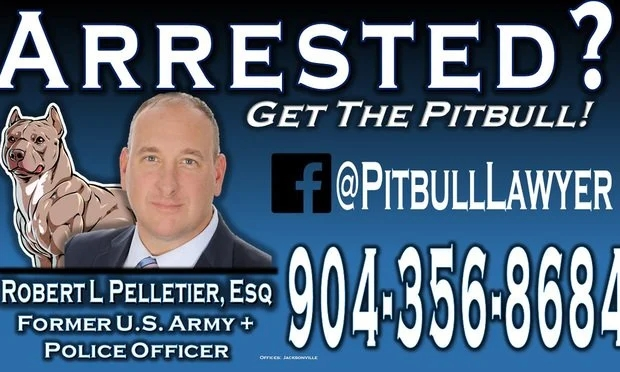
\includegraphics[width=0.5\linewidth,height=\textheight,keepaspectratio]{../img/Pitbull2.jpg}

}

\caption{Pelletier ad}

\end{figure}%

In his \href{../exhibits/Pelletier-Answer.pdf}{answer} to the Bar
complaint, Pelletier to the Bar complaint, Pelletier asserted that he
``was unaware of said case law until recently. Furthermore, Respondent
was unaware that using a nickname such as ``Pitbull'' was a violation of
The Florida Bar Rules.'' He also contended that ``The Florida Bar
rule(s) sited {[}sic{]} violate the first amendment freedom of speech
section.'' He ultimately entered a
\href{../exhibits/Pelletier-GuiltyPlea.pdf}{guilty plea} and received a
\href{../exhibits/Pelletier-RefereeReport.pdf}{reprimand}.

\subsection{Hunter v. Virginia State Bar, 744 S.E.2d 611 (Va.
2013)}\label{hunter-v.-virginia-state-bar-744-s.e.2d-611-va.-2013}

\subsubsection{Opinion by Justice Cleo E.
Powell}\label{opinion-by-justice-cleo-e.-powell}

In this appeal of right by an attorney from a Virginia State Bar
(``VSB'') disciplinary proceeding, we consider whether an attorney's
blog posts are commercial speech, whether an attorney may discuss public
information related to a client without the client's consent, and
whether the panel ordered the attorney to post a disclaimer that is
insufficient under Rule 7.2(a)(3) of the Virginia Rules of Professional
Conduct.

\subsubsection{I. Facts and Proceedings}\label{i.-facts-and-proceedings}

Horace Frazier Hunter, an attorney with the law firm of Hunter \&
Lipton, PC, authors a trademarked blog titled ``This Week in Richmond
Criminal Defense,'' which is accessible from his law firm's website,
www.hunterlipton.com. This blog, which is not interactive, contains
posts discussing a myriad of legal issues and cases, although the
overwhelming majority are posts about cases in which Hunter obtained
favorable results for his clients. Nowhere in these posts or on his
website did Hunter include disclaimers.

As a result of Hunter's blog posts on his website, the VSB launched an
investigation. During discussions with the VSB about whether his blog
constituted legal advertising, Hunter wrote a letter to the VSB offering
to post \emph{a disclaimer} on \emph{one page} of his website:

\begin{quote}
``\emph{This Week in Richmond Criminal Defense} is not an
advertisement{[};{]} it is a blog. The views and opinions expressed on
this blog are solely those of attorney Horace F. Hunter. The purpose of
these articles is to inform the public regarding various issues
involving the criminal justice system and should not be construed to
suggest a similar outcome in any other case.''
\end{quote}

However, the negotiations stalled and no disclaimers were posted at that
time.

On March 24, 2011, the VSB charged Hunter with violating Rules 7.1, 7.2,
7.5, and 1.6 by his posts on this blog. Specifically, the VSB argued
that he violated rules 7.1 and 7.2 because his blog posts discussing his
criminal cases were inherently misleading as they lacked disclaimers.
The VSB also asserted that Hunter violated Rule 1.6 by revealing
information that could embarrass or likely be detrimental to his former
clients by discussing their cases on his blog without their consent.

In a hearing on October 18, 2011, the VSB presented evidence of Hunter's
alleged violations. The VSB presented a former client who testified that
he did not consent to information about his cases being posted on
Hunter's blog and believed that the information posted was embarrassing
or detrimental to him, despite the fact that all such information had
previously been revealed in court. The VSB investigator testified that
other former clients felt similarly. The VSB also entered all of the
blog posts Hunter had posted on his blog to date. At that time, none of
the posts entered contained disclaimers. Of these thirty unique posts,
only five discussed legal, policy issues. The remaining twenty-five
discussed cases. Hunter represented the defendant in twenty-two of these
cases and identified that fact in the posts. In nineteen of these
twenty-two posts, Hunter also specifically named his law firm. One of
these posts described a case where a family hired Hunter to represent
them in a wrongful death suit and the remaining twenty-one of these
posts described criminal cases. In every criminal case described,
Hunter's clients were either found not guilty, plea bargained to an
agreed upon disposition, or had their charges reduced or dismissed.

At the hearing, Hunter testified that he has many reasons for writing
his blog---including marketing, creation of a community presence for his
firm, combatting any public perception that defendants charged with
crimes are guilty until proven innocent, and showing commitment to
criminal law. Hunter stated that he had offered to post a disclaimer on
his blog, but the offered disclaimer was not satisfactory to the VSB.
Hunter admitted that he only blogged about his cases that he won. He
also told the VSB that he believed that using the client's name is
important to give an accurate description of what happened. Hunter told
the VSB that he did not obtain consent from his clients to discuss their
cases on his blog because all the information that he posted was public
information.

Following the hearing, the VSB held that Hunter violated Rule 1.6 by
``disseminating client confidences'' obtained in the course of
representation without consent to post. Specifically, the VSB found that
the information in Hunter's blog posts ``would be embarrassing or be
likely to be detrimental'' to clients and he did not receive consent
from his clients to post such information. The VSB further held that
Hunter violated Rule 7.1. The VSB's conclusion that Hunter's website
contained legal advertising was based on its factual finding that ``the
postings of {[}Hunter's{]} case wins on his webpage advertised
cumulative case results.'' Moreover, the VSB found that at least one
purpose of the website was commercial. The VSB further held that he
violated Rule 7.2 by ``disseminating case results in advertising without
the required disclaimer'' because the one that he proposed to the VSB
was insufficient. The VSB imposed a public admonition with terms
including a requirement that he remove case specific content for which
he has not received consent and post a disclaimer that complies with
Rule 7.2(a)(3) on all case-related posts.

Hunter appealed to a three judge panel of the circuit court and the
court heard argument. The court disagreed with Hunter that \emph{de
novo} was the proper standard of review and instead applied the
following standard: ``whether the decision is contrary to the law or
whether there is substantial evidence in the record upon which the
district committee could reasonably have found as it did.'' The court
further ruled that the VSB's interpretation of Rule 1.6 violated the
First Amendment and dismissed that charge. The court held VSB's
interpretation of Rules 7.1 and 7.2 do not violate the First Amendment
and that the record contained substantial evidence to support the VSB's
determination that Hunter had violated those rules. The court imposed a
public admonition and required Hunter to post the following disclaimer:
``Case results depend upon a variety of factors unique to each case.
Case results do not guarantee or predict a similar result in any future
case.'' This appeal followed.

\subsubsection{II. Analysis}\label{ii.-analysis}

\paragraph{A. Whether ``the Ruling of the Circuit Court finding a
violation of Rules 7.1(a)(4) and 7.2(a)(3) conflicts with the First
Amendment to the Constitution of the United
States.''}\label{a.-whether-the-ruling-of-the-circuit-court-finding-a-violation-of-rules-7.1a4-and-7.2a3-conflicts-with-the-first-amendment-to-the-constitution-of-the-united-states.}

Rule 7.1(a)(4), which is the specific portion of the Rule that the VSB
argued that Hunter violated, states:

\begin{quote}
(a) A lawyer shall not, on behalf of the lawyer or any other lawyer
affiliated with the lawyer or the firm, use or participate in the use of
any form of public communication if such communication contains a false,
fraudulent, misleading, or deceptive statement or claim. For example, a
communication violates this Rule if it:
\end{quote}

\begin{quote}
\begin{quote}
(4) is likely to create an unjustified expectation about results the
lawyer can achieve, or states or implies that the lawyer can achieve
results by means that violate the Rules of Professional Conduct or other
law.
\end{quote}
\end{quote}

The VSB also argues that Hunter violated the following subsection of
Rule 7.2(a)(3):

\begin{quote}
(a) Subject to the requirements of Rules 7.1 and 7.3, a lawyer may
advertise services through written, recorded, or electronic
communications, including public media. In the determination of whether
an advertisement violates this Rule, the advertisement shall be
considered in its entirety, including any qualifying statements or
disclaimers contained therein. Notwithstanding the requirements of Rule
7.1, an advertisement violates this Rule if it:
\end{quote}

\begin{quote}
\begin{quote}
(3) advertises specific or cumulative case results, without a disclaimer
that (i) puts the case results in a context that is not misleading; (ii)
states that case results depend upon a variety of factors unique to each
case; and (iii) further states that case results do not guarantee or
predict a similar result in any future case undertaken by the lawyer.
The disclaimer shall precede the communication of the case results. When
the communication is in writing, the disclaimer shall be in bold type
face and uppercase letters in a font size that is at least as large as
the largest text used to advertise the specific or cumulative case
results and in the same color and against the same colored background as
the text used to advertise the specific or cumulative case results.
\end{quote}
\end{quote}

In response to these allegations, Hunter contends that speech concerning
the judicial system is ``quintessentially `political speech'\,'' which
is within the marketplace of ideas. Hunter asserts that the Supreme
Court of the United States has twice declined to answer whether
political speech is transformed into commercial speech simply because
one of multiple motives is commercial. Specifically, he argues that his
blog posts are not commercial because

\begin{quote}
(1) the {[}Supreme Court of the United States'{]} formal commercial
speech definitions focus heavily on whether the speech does \emph{no
more} than propose a commercial transaction; (2) the {[}Supreme Court of
the United States'{]} commercial speech decisions, to the extent that
they discuss motivation at all, have focused on whether the speech is
\emph{solely} driven by commercial interest; (3) the {[}Supreme Court of
the United States{]} has repeatedly insisted that the existence of a
commercial motivation does not disqualify speech from the heightened
scrutiny protection it would otherwise deserve; (4) the {[}Supreme Court
of the United States{]} has warned that when commercial and political
elements of speech are inextricably intertwined, the heightened
protection applicable to the political the constitutional policy
arguments that undergird the reduction of protection for commercial
speech have no persuasive force when the content of the speech is
political.
\end{quote}

The VSB responds that Hunter's blog posts are inherently misleading
commercial speech.

``Whether the inherent character of a statement places it beyond the
protection of the First Amendment is a question of law over which this
Court exercises de novo review.'' An appellate Court must independently
examine the entire record in First Amendment cases to ensure that ``\,`a
forbidden intrusion on the field of free expression'\,'' has not
occurred.

Turning to Hunter's argument that his blog posts are political, rather
than commercial, speech, we note that ``the existence of `commercial
activity, in itself, is no justification for narrowing the protection of
expression secured by the First Amendment.'\,'' However, when speech
that is both commercial and political is combined, the resulting speech
is not automatically entitled to the level of protections afforded
political speech.

While it is settled that attorney advertising is commercial speech,
\emph{Bates} and its progeny were decided in the era of traditional
media. In recent years, however, advertising has taken to new forms such
as websites, blogs, and other social media forums, like Facebook and
Twitter.

Thus, we must examine Hunter's speech to determine whether it is
commercial speech, specifically, lawyer advertising.

\begin{quote}
Advertising, like all public expression, may be subject to reasonable
regulation that serves a legitimate public interest. To the extent that
commercial activity is subject to regulation, the relationship of speech
to that activity may be one factor, among others, to be considered in
weighing the First Amendment interest against the governmental interest
alleged. Advertising is not thereby stripped of all First Amendment
protection. The relationship of speech to the marketplace of products or
of services does not make it valueless in the marketplace of ideas.
\end{quote}

Simply because the speech is an advertisement, references a specific
product, or is economically motivated does not necessarily mean that it
is commercial speech. ``The combination of \emph{all} these
characteristics, however, provides strong support for the conclusion
that {[}some blog posts{]} are properly characterized as commercial
speech'' even though they also discuss issues important to the public.

Certainly, not all advertising is necessarily commercial, e.g., public
service announcements.However, all commercial speech is necessarily
advertising. Indeed, the Supreme Court of the United States has said
that ``the diverse motives, means, and messages of advertising may make
speech `commercial' in widely varying degrees.''

Here, Hunter's blog posts, while containing some political commentary,
are commercial speech. Hunter has admitted that his motivation for the
blog is at least in part economic. The posts are an advertisement in
that they predominately describe cases where he has received a favorable
result for his client. He unquestionably references a specific product,
i.e., his lawyering skills as twenty-two of his twenty-five case related
posts describe cases that he has successfully handled. Indeed, in
nineteen of these posts, he specifically named his law firm in addition
to naming himself as counsel.

Moreover, the blog is on his law firm's commercial website rather than
an independent site dedicated to the blog. The website uses the same
frame for the pages openly soliciting clients as it does for the blog,
including the firm name, a photograph of Hunter and his law partner, and
a ``contact us'' form. The homepage of the website on which Hunter
posted his blog states only:

\begin{quote}
Do you need Richmond attorneys?
\end{quote}

\begin{quote}
Hunter \& Lipton, CP sic is a law practice in Richmond, Virginia
specializing in litigation matters from administrative agency hearings
to serious criminal cases. As experienced Richmond attorneys, we bring a
genuine desire to help those who find themselves in difficult
situations. Our partnership was founded on the idea that everyone, no
matter what the circumstance, deserves a zealous advocate to fight on
his or her behalf.
\end{quote}

\begin{quote}
People make mistakes, and may even find themselves in situations not of
their own making. And for these people, the system can be
extraordinarily unforgiving and unjust---but you do not have to face
this system alone.
\end{quote}

\begin{quote}
If you find yourself in a difficult legal situation, the Richmond
attorneys of Hunter \& Lipton, LLP would consider it a privilege to
represent you. Please contact our office with any questions or to
schedule a consultation.
\end{quote}

This non-interactive blog does not allow for discourse about the cases,
as non-commercial commentary often would by allowing readers to post
comments. Instead, in furtherance of his commercial pursuit, Hunter
invites the reader to ``contact us'' the same way one seeking legal
representation would contact the firm through the website.

Thus, the inclusion of five generalized, legal posts and three
discussions about cases that he did not handle on his non-interactive
blog, no more transform Hunter's otherwise self-promotional blog posts
into political speech, ``than opening sales presentations with a prayer
or a Pledge of Allegiance would convert them into religious or political
speech.'' Indeed, unlike situations and topics where the subject matter
is inherently, inextricably intertwined, Hunter chose to comingle
sporadic political statements within his self-promoting blog posts in an
attempt to camouflage the true commercial nature of his blog.
``Advertisers should not be permitted to immunize false or misleading
product information from government regulation simply by including
references to public issues.'' When considered as a whole, the
economically motivated blog overtly proposes a commercial transaction
that is an advertisement of a specific product.

Having determined that Hunter's blog posts discussing his cases are
commercial speech,

\begin{quote}
we must determine whether the expression is protected by the First
Amendment. For commercial speech to come within that provision, it at
least must concern lawful activity and not be misleading. Next, we ask
whether the asserted governmental interest is substantial. If both
inquiries yield positive answers, we must determine whether the
regulation directly advances the governmental interest asserted, and
whether it is not more extensive than is necessary to serve that
interest.
\end{quote}

The VSB does not contend, nor does the record indicate, that Hunter's
posts do not concern lawful activity; rather, the VSB argues that the
posts are inherently misleading. While we do not hold that the blog
posts are inherently misleading, we do conclude that they have the
potential to be misleading. ``Because the public lacks sophistication
concerning legal services, misstatements that might be overlooked or
deemed unimportant in other advertising may be found quite inappropriate
in legal advertising.'' Of the thirty posts that were on his blog at the
time of the VSB hearing, twenty-two posts named himself as counsel and
discussed cases that he handled. With one exception, in all of these
posts, he described the successful results that he obtained for his
clients. While the States may place an absolute prohibition on
inherently misleading advertising, ``the States may not place an
absolute prohibition on certain types of potentially misleading
information, if the information also may be presented in a way that is
not deceptive.'' Here, the VSB's own remedy of requiring Hunter to post
disclaimers on his blog posts demonstrates that the information could be
presented in a way that is not misleading or deceptive.

Thus, we must examine whether the VSB has a substantial governmental
interest in regulating these blog posts. The Supreme Court of the United
States has recognized that ``\,`if the naiveté of the public will cause
advertising by attorneys to be misleading, then it is the bar's role to
assure that the populace is sufficiently informed as to enable it to
place advertising in its proper perspective.'\,'' Indeed, the Supreme
Court of the United States expressed concern that the public may lack
the sophistication to discern misstatements as to the quality of a
lawyer's services. Therefore, the VSB has a substantial governmental
interest in protecting the public from an attorney's self-promoting
representations that could lead the public to mistakenly believe that
they are guaranteed to obtain the same positive results if they were to
hire Hunter.

Because the VSB's governmental interest is substantial, we must now
determine ``whether the regulation directly advances the governmental
interest asserted.'' The VSB's regulations permit blog posts that
discuss specific or cumulative case results but require a disclaimer to
explain to the public that no results are guaranteed. Rules 7.1 and 7.2.
This requirement directly advances the VSB's governmental interest.

Finally, we must determine whether the VSB's regulations are no more
restrictive than necessary. The Supreme Court of the United States has
approved the use of disclaimers or explanations. The disclaimers
mandated by the VSB

\begin{quote}
shall precede the communication of the case results. When the
communication is in writing, the disclaimer shall be in bold type face
and uppercase letters in a font size that is at least as large as the
largest text used to advertise the specific or cumulative case results
and in the same color and against the same colored background as the
text used to advertise the specific or cumulative case results.
\end{quote}

Rule 7.2(a)(3). This requirement ensures that the disclaimer is
noticeable and would be connected to each post so that any member of the
public who may use the website addresses to directly access Hunter's
posts would be in a position to see the disclaimer. Therefore, we hold
that the disclaimers required by the VSB are ``not more extensive than
is necessary to serve that interest.''

Hunter's blog posts discuss lawful activity and are not inherently
misleading, but the VSB has asserted a substantial governmental interest
to protect the public from potentially misleading lawyer advertising.
These regulations directly advance this interest and are not more
restrictive than necessary, unlike outright bans on advertising. We thus
conclude that the VSB's Rules 7.1 and 7.2 do not violate the First
Amendment. As applied to Hunter's blog posts, they are constitutional
and the panel did not err.

\paragraph{B. Whether the circuit court erred in holding that the VSB's
application of Rule 1.6 to Hunter's blog violated his First Amendment
rights.}\label{b.-whether-the-circuit-court-erred-in-holding-that-the-vsbs-application-of-rule-1.6-to-hunters-blog-violated-his-first-amendment-rights.}

Rule 1.6(a) states, that with limited exceptions,

\begin{quote}
a lawyer shall not reveal information protected by the attorney-client
privilege under applicable law or other information gained in the
professional relationship that the client has requested be held
inviolate or the disclosure of which would be embarrassing or would be
likely to be detrimental to the client unless the client consents after
consultation, except for disclosures that are impliedly authorized in
order to carry out the representation.
\end{quote}

The VSB argues that the circuit court erred in holding that its
interpretation of Rule 1.6 violates the First Amendment and that Hunter
violated that rule by disclosing potentially embarrassing information
about his clients on his blog ``in order to advance his personal
economic interests.'' VSB argues that lawyers, as officers of the Court,
are prohibited from engaging in speech that might otherwise be
constitutionally protected. Thus, the VSB's interpretation of Rule 1.6
involves two types of information: 1) that which is protected by the
attorney-client privilege, and 2) that which is public information but
is embarrassing or likely to be detrimental to the client. Hunter is
charged with disseminating the later type of information. In response to
these allegations, Hunter argues that the VSB's interpretation of Rule
1.6 is unconstitutional because the matters discussed in his blogs had
previously been revealed in public judicial proceedings and, therefore,
as concluded matters, were protected by the First Amendment. Thus, we
are called upon to answer whether the state may prohibit an attorney
from discussing information about a client or former client that is not
protected by attorney-client privilege without express consent from that
client. We agree with Hunter that it may not.

The cases cited by VSB in support of its position differ from this case
in a substantial way; the cases relied upon by VSB involve pending
proceedings. It is settled that attorney speech about public information
from cases is protected by the First Amendment, but it may be regulated
if it poses a substantial likelihood of materially prejudicing a
\emph{pending} case.

``A presumption of openness inheres in the very nature of a criminal
trial under our system of justice.'' Moreover,

\begin{quote}
a trial is a public event. What transpires in the court room is public
property. If a transcript of the court proceedings had been published,
we suppose none would claim that the judge could punish the publisher
for contempt. And we can see no difference though the conduct of the
attorneys, of the jury or even of the judge himself, may have reflected
on the court. Those who see and hear what transpired can report it with
impunity. There is no special perquisite of the judiciary which enables
it, as distinguished from other institutions of democratic government,
to suppress, edit, or censor events which transpire in proceedings
before it.
\end{quote}

All of Hunter's blog posts involved cases that had been concluded.
Moreover, the VSB concedes that all of the information that was
contained within Hunter's blog was public information and would have
been protected speech had the news media or others disseminated it. In
deciding whether the circuit court erred, we are required to make our
``own inquiry into the imminence and magnitude of the danger said to
flow from the particular utterance and then to balance the character of
the evil, as well as its likelihood, against the need for free and
unfettered expression.'' ``At the very least, the cases recognize that
disciplinary rules governing the legal profession cannot punish activity
protected by the First Amendment, and that First Amendment protection
survives even when the attorney violates a disciplinary rule he swore to
obey when admitted to the practice of law.'' The VSB's interpretation of
Rule 1.6 fails these standards even when we

\begin{quote}
balance ``whether the `practice in question furthers an important or
substantial governmental interest unrelated to the suppression of
expression' and whether `the limitation of First Amendment freedoms is
no greater than is necessary or essential to the protection of the
particular governmental interest involved,'\,''
\end{quote}

State action that punishes the publication of truthful information can
rarely survive constitutional scrutiny.

The VSB argues that it can prohibit an attorney from repeating truthful
information made in a public judicial proceeding even though others can
disseminate this information because an attorney repeating it could
inhibit clients from freely communicating with their attorneys or
because it would undermine public confidence in the legal profession.
Such concerns, however, are unsupported by the evidence. To the extent
that the information is aired in a public forum, privacy considerations
must yield to First Amendment protections. In that respect, a lawyer is
no more prohibited than any other citizen from reporting what transpired
in the courtroom. Thus, the circuit court did not err in concluding that
the VSB's interpretation of Rule 1.6 violated the First Amendment.

\paragraph{C. Whether the circuit court erred in requiring Hunter to
post a disclaimer on his website that does not comply with the
requirements of Rule 7.2(3) and therefore does not eliminate the
misleading nature of his blog
posts.}\label{c.-whether-the-circuit-court-erred-in-requiring-hunter-to-post-a-disclaimer-on-his-website-that-does-not-comply-with-the-requirements-of-rule-7.23-and-therefore-does-not-eliminate-the-misleading-nature-of-his-blog-posts.}

The VSB argues that the single disclaimer that the circuit court ordered
Hunter to post on his blog was insufficient to comport with Rule
7.2(a)(3) because it did not eliminate the misleading nature of the
posts.

As we have already concluded, Hunter's blogs are commercial speech and,
thus, constitute lawyer advertising. When advertising cumulative or
specific case results, Rule 7.2 requires that a disclaimer

\begin{quote}
shall be in bold type face and uppercase letters in a font size that is
at least as large as the largest text used to advertise the specific or
cumulative case results and in the same color and against the same
colored background as the text used to advertise the specific or
cumulative case results.
\end{quote}

Rule 7.2(a)(3).

Here, the VSB required Hunter to post a disclaimer that complies with
Rule 7.2(a)(3) on \emph{all} case-related posts. This means that
Hunter's disclaimers ``shall be in bold type face and uppercase letters
in a font size that is at least as large as the largest text used to
advertise the specific or cumulative case results and in the same color
and against the same colored background as the text used to advertise
the specific or cumulative case results.'' Rule 7.2(a)(3). The circuit
court, however, imposed the following disclaimer to be posted once:
``Case results depend upon a variety of factors unique to each case.
Case results do not guarantee or predict a similar result in any future
case.''

While the substantive meaning of the imposed disclaimer may conform to
the requirements stated in Rule 7.2(a)(3)(i) through (iii), it
nevertheless is less than what the rule requires. In contrast to the
committee's determination, there is no provision in the circuit court's
order requiring that the disclaimer be formatted and presented in the
manner required by Rule 7.2(a)(3), and the text of the disclaimer
prescribed by the circuit court is not itself formatted and presented in
that manner. Even so, Hunter does not argue that the disclaimer required
by the circuit court is an appropriate, less restrictive means of
regulating his speech and, therefore, we decline to so hold. Based on
the arguments presented to it, the circuit court erred by imposing a
disclaimer that conflicted with the rule.

\subsubsection{III. Conclusion}\label{iii.-conclusion}

For the foregoing reasons, we hold that Hunter's blog posts are
potentially misleading commercial speech that the VSB may regulate. We
further hold that circuit court did not err in determining that the
VSB's interpretation of Rule 1.6 violated the First Amendment. Finally,
we hold that because the circuit court erred in imposing one disclaimer
did not fully comply with Rule 7.2(a)(3), we reverse and remand for
imposition of disclaimers that fully comply with that Rule.

\subsubsection{Justice LEMONS, with whom Justice McCLANAHAN joins,
dissenting in
part.}\label{justice-lemons-with-whom-justice-mcclanahan-joins-dissenting-in-part.}

I agree with the majority's resolution of the Rule 1.6 issue. However, I
dissent from the majority's determination that Hunter is guilty of
violating Rules 7.1(a)(4) and 7.2(a)(3) and that Hunter must post a
disclaimer that complies with Rule 7.2(a)(3).

Rule 7.1 governs communications concerning a lawyer's services. Rule
7.1(a)(4) states:

\begin{quote}
(a) A lawyer shall not, on behalf of the lawyer or any other lawyer
affiliated with the lawyer or the firm, use or participate in the use of
any form of public communication if such communication contains a false,
fraudulent, misleading, or deceptive statement or claim. For example, a
communication violates this Rule if it:
\end{quote}

\begin{quote}
\begin{quote}
(4) is likely to create an unjustified expectation about results the
lawyer can achieve, or states or implies that the lawyer can achieve
results by means that violate the Rules of Professional Conduct or other
law.
\end{quote}
\end{quote}

Rule 7.2 is only applicable to advertisements. Rule 7.2(a)(3) states:

\begin{quote}
(a) Subject to the requirements of Rules 7.1 and 7.3, a lawyer may
advertise services through written, recorded, or electronic
communications, including public media. In the determination of whether
an advertisement violates this Rule, the advertisement shall be
considered in its entirety, including any qualifying statements or
disclaimers contained therein. Notwithstanding the requirements of Rule
7.1, an advertisement violates this Rule if it:
\end{quote}

\begin{quote}
\begin{quote}
(3) advertises specific or cumulative case results, without a disclaimer
that (i) puts the case results in a context that is not misleading; (ii)
states that case results depend upon a variety of factors unique to each
case; and (iii) further states that case results do not guarantee or
predict a similar result in any future case undertaken by the lawyer.
The disclaimer shall precede the communication of the case results. When
the communication is in writing, the disclaimer shall be in bold type
face and uppercase letters in a font size that is at least as large as
the largest text used to advertise the specific or cumulative case
results and in the same color and against the same colored background as
the text used to advertise the specific or cumulative case results.
\end{quote}
\end{quote}

Hunter's blog contains articles about legal and policy issues in the
news, as well as detailed descriptions of criminal trials, the majority
of which are cases where Hunter was the defense attorney. The articles
also contain Hunter's commentary and critique of the criminal justice
system. He uses the case descriptions to illustrate his views.

\subsubsection{The First Amendment}\label{the-first-amendment}

I believe that the articles on Hunter's blog are political speech that
is protected by the First Amendment. The Bar concedes that if Hunter's
blog is political speech, the First Amendment protects him and the Bar
cannot force Hunter to post an advertising disclaimer on his blog.

Speech concerning the criminal justice system has always been viewed as
political speech. ``It would be difficult to single out any aspect of
government of higher concern and importance to the people than the
manner in which criminal trials are conducted.'' As political speech,
Hunter uses his blog to give detailed descriptions of how criminal
trials in Virginia are conducted. He notes how the acquittal of some of
his clients has exposed flaws in the criminal justice system.

The majority asserts that because Hunter only discusses his victories,
his blog is commercial. The majority does not give sufficient credit to
the fact that Hunter uses the outcome of his cases to illustrate his
views of the system. Hunter testified that one of the reasons he
maintained the blog was to combat ``the public perception that is
clearly on the side that people are guilty until they're proven
innocent.'' For example, when discussing one of the cases where his
client was found not guilty, he concludes the post by explaining that
this case is an ``example of how innocent people are often accused of
committing some of the most serious crimes. That is why it is important
not to judge the guilt of an individual until all the evidence has been
presented both for and against him.''

The majority compares Hunter's detailed discussion of criminal trials
and how these outcomes illustrate the need to hold government to its
burden of proof, with ``opening a sales presentation{[}{]} with a prayer
or a Pledge of Allegiance.'' The majority proposes that his blog is not
transformed into political speech simply because he included eight posts
about legal issues and cases he was not involved in. However, the
twenty-two posts discussing criminal trials in Virginia are political
speech in their own right, and are not dependent upon the content of the
other eight posts.

The majority also focuses on the location of Hunter's blog, and asserts
that because the blog is accessed through the law firm's website and is
not interactive, that demonstrates the blog is commercial in nature.
While going through the law firm's website is one way to access the
blog, it is also possible to go directly to the blog without navigating
through the firm's website. Further, the fact that the blog is not
interactive in no way commercializes the speech.

Many businesses have websites. It is not uncommon for websites to
include links to related news articles or editorials. Merely because an
article may be accessed through a commercial portal does not change the
content of the article. It is the content of speech and the motivation
of the speaker that determines the level of protection to which speech
is entitled.

Hunter conceded that one of the purposes of the blog was marketing.
Although the United States Supreme Court has never clearly decided
whether political speech is transformed into commercial speech because
one of the multiple motivations of the speaker is marketing and
self-promotion, its jurisprudence leads to the conclusion that Hunter's
speech is not commercial.

The traditional test for determining whether speech is commercial is if
the speech ``does \emph{no more than} propose a commercial
transaction.'' Hunter's articles clearly do more than propose a
commercial transaction. They contain detailed discussions of criminal
trials in this Commonwealth, and Hunter's commentary and critique of the
criminal justice system.

The United States Supreme Court has held that commercial speech is
``expression related \emph{solely} to the economic interests of the
speaker and its audience.'' Marketing is not Hunter's sole motivation
for maintaining this blog. As discussed above, one of Hunter's
motivations in maintaining the blog is to disseminate information about
``the criminal justice system, the criminal trials and the manner in
which the government prosecutes its citizens.''

Even if marketing was Hunter's sole motivation, economic motivation
cannot be the basis for determining whether otherwise political speech
is protected. The United States Supreme Court recognized in
\emph{Pittsburgh Press Co}. that merely having some economic motivation
does not create a basis for regulation. ``If a newspaper's profit motive
were determinative, all aspects of its operations---from the selection
of news stories to the choice of editorial position---would be subject
to regulation if it could be established that they were conducted with a
view toward increased sales. Such a basis for regulation clearly would
be incompatible with the First Amendment.''

The mere existence of some commercial motivation does not change
otherwise political speech into commercial speech. ``Speech does not
lose its First Amendment protection because money is spent to project
it, as in a paid advertisement of one form or another.'' In discussing
the economic motivations at issue in \emph{Sorrell v. IMS Health, Inc.},
the United States Supreme Court recognized that ``while the burdened
speech results from an economic motive, so too does a great deal of
vital expression.''

Even if there is some commercial content to Hunter's speech, any
commercial content is intertwined with political speech. When commercial
and political elements are intertwined in speech, the heightened
scrutiny test must apply to all of the speech.

\begin{quote}
It is not clear that a professional's speech is necessarily commercial
whenever it relates to that person's financial motivation for speaking.
But even assuming, without deciding, that such speech in the abstract is
indeed merely ``commercial,'' we do not believe that the speech retains
its commercial character when it is inextricably intertwined with
otherwise fully protected speech. Our lodestars in deciding what level
of scrutiny to apply to a compelled statement must be the nature of the
speech taken as a whole and the effect of the compelled statement
thereon.
\end{quote}

In this case, the policies the Bar advances have no persuasive force
when applied to Hunter's blog. The purposes of Rules 7.1 and 7.2 are to
protect the public from misleading communications and advertisements
concerning a lawyer's services. Hunter's articles contain detailed
descriptions of the trials, along with his commentary on the criminal
justice system. The Bar produced no evidence that anyone has found
Hunter's articles to be misleading. There appears to be little benefit,
if any, to the public by requiring Hunter to post a disclaimer that
concedes his articles are advertisements. Hunter disagrees that his
articles are advertisements, and claims they are political speech. He
objects to cheapening his political speech by denominating it as
advertisement material.

Accordingly, I would hold that Hunter's speech is political, is entitled
to the heightened scrutiny test, and that he cannot be forced to include
the advertising disclaimer under Rule 7.2 that the Bar seeks to force
upon his writings.

\section{Solicitation}\label{solicitation}

\subsection{Model Rules of Professional Conduct, Rule
7.3}\label{model-rules-of-professional-conduct-rule-7.3}

\subsubsection{Solicitation of Clients}\label{solicitation-of-clients}

(a) ``Solicitation'' or ``solicit'' denotes a communication initiated by
or on behalf of a lawyer or law firm that is directed to a specific
person the lawyer knows or reasonably should know needs legal services
in a particular matter and that offers to provide, or reasonably can be
understood as offering to provide, legal services for that matter.

(b) A lawyer shall not solicit professional employment by live
person-to-person contact when a significant motive for the lawyer's
doing so is the lawyer's or law firm's pecuniary gain, unless the
contact is with a:

\begin{itemize}
\item
  (1) lawyer;
\item
  (2) person who has a family, close personal, or prior business or
  professional relationship with the lawyer or law firm; or
\item
  (3) person who routinely uses for business purposes the type of legal
  services offered by the lawyer.
\end{itemize}

(c) A lawyer shall not solicit professional employment even when not
otherwise prohibited by paragraph (b), if:

\begin{itemize}
\item
  (1) the target of the solicitation has made known to the lawyer a
  desire not to be solicited by the lawyer; or
\item
  (2) the solicitation involves coercion, duress or harassment.
\end{itemize}

(d) This Rule does not prohibit communications authorized by law or
ordered by a court or other tribunal.

(e) Notwithstanding the prohibitions in this Rule, a lawyer may
participate with a prepaid or group legal service plan operated by an
organization not owned or directed by the lawyer that uses live
person-to-person contact to enroll members or sell subscriptions for the
plan from persons who are not known to need legal services in a
particular matter covered by the plan.

\subsection{Model Rules of Professional Conduct, Rule
7.6}\label{model-rules-of-professional-conduct-rule-7.6}

\subsubsection{Political Contributions to Obtain Legal Engagements or
Appointments by
Judges}\label{political-contributions-to-obtain-legal-engagements-or-appointments-by-judges}

A lawyer or law firm shall not accept a government legal engagement or
an appointment by a judge if the lawyer or law firm makes a political
contribution or solicits political contributions for the purpose of
obtaining or being considered for that type of legal engagement or
appointment.

\subsection{NAACP v. Button, 371 U.S. 415
(1963)}\label{naacp-v.-button-371-u.s.-415-1963}

\subsubsection{MR. JUSTICE BRENNAN delivered the opinion of the
Court.}\label{mr.-justice-brennan-delivered-the-opinion-of-the-court.}

This case originated in companion suits by the National Association for
the Advancement of Colored People, Inc.~(NAACP), and the NAACP Legal
Defense and Educational Fund, Inc.~(Defense Fund), brought in 1957 in
the United States District Court for the Eastern District of Virginia.
The suits sought to restrain the enforcement of Chapters 31, 32, 33, 35
and 36 of the Virginia Acts of Assembly, 1956 Extra Session, on the
ground that the statutes, as applied to the activities of the
plaintiffs, violated the Fourteenth Amendment. A three-judge court
convened pursuant to 28 U. S. C. § 2281, after hearing evidence and
making fact-findings, struck down Chapters 31, 32 and 35 but abstained
from passing upon the validity of Chapters 33 and 36 pending an
authoritative interpretation of these statutes by the Virginia courts.
The complainants thereupon petitioned in the Circuit Court of the City
of Richmond to declare Chapters 33 and 36 inapplicable to their
activities, or, if applicable, unconstitutional. The record in the
Circuit Court was that made before the three-judge court supplemented by
additional evidence. The Circuit Court held the chapters to be both
applicable and constitutional. The holding was sustained by the Virginia
Supreme Court of Appeals as to Chapter 33, but reversed as to Chapter
36, which was held unconstitutional under both state and federal law.
Thereupon the Defense Fund returned to the Federal District Court, where
its case is presently pending, while the NAACP filed the instant
petition. We granted certiorari, and ordered reargument this Term. The
only issue before us is the constitutionality of Chapter 33 as applied
to the activities of the NAACP.

There is no substantial dispute as to the facts; the dispute centers
about the constitutionality under the Fourteenth Amendment of Chapter
33, as construed and applied by the Virginia Supreme Court of Appeals to
include NAACP's activities within the statute's ban against ``the
improper solicitation of any legal or professional business.''

The NAACP was formed in 1909 and incorporated under New York law as a
nonprofit membership corporation in 1911. It maintains its headquarters
in New York and presently has some 1,000 active unincorporated branches
throughout the Nation. The corporation is licensed to do business in
Virginia, and has 89 branches there. The Virginia branches are organized
into the Virginia State Conference of NAACP Branches (the Conference),
an unincorporated association, which in 1957 had some 13,500 members.
The activities of the Conference are financed jointly by the national
organization and the local branches from contributions and membership
dues. NAACP policy, binding upon local branches and conferences, is set
by the annual national convention.

The basic aims and purposes of NAACP are to secure the elimination of
all racial barriers which deprive Negro citizens of the privileges and
burdens of equal citizenship rights in the United States. To this end
the Association engages in extensive educational and lobbying
activities. It also devotes much of its funds and energies to an
extensive program of assisting certain kinds of litigation on behalf of
its declared purposes. For more than 10 years, the Virginia Conference
has concentrated upon financing litigation aimed at ending racial
segregation in the public schools of the Commonwealth.

The Conference ordinarily will finance only cases in which the assisted
litigant retains an NAACP staff lawyer to represent him. The Conference
maintains a legal staff of 15 attorneys, all of whom are Negroes and
members of the NAACP. The staff is elected at the Conference's annual
convention. Each legal staff member must agree to abide by the policies
of the NAACP, which, insofar as they pertain to professional services,
limit the kinds of litigation which the NAACP will assist. Thus the
NAACP will not underwrite ordinary damages actions, criminal actions in
which the defendant raises no question of possible racial
discrimination, or suits in which the plaintiff seeks separate but equal
rather than fully desegregated public school facilities. The staff
decides whether a litigant, who may or may not be an NAACP member, is
entitled to NAACP assistance. The Conference defrays all expenses of
litigation in an assisted case, and usually, although not always, pays
each lawyer on the case a per diem fee not to exceed \$60, plus
out-of-pocket expenses. The assisted litigant receives no money from the
Conference or the staff lawyers. The staff member may not accept, from
the litigant or any other source, any other compensation for his
services in an NAACP-assisted case. None of the staff receives a salary
or retainer from the NAACP; the per diem fee is paid only for
professional services in a particular case. This per diem payment is
smaller than the compensation ordinarily received for equivalent private
professional work. The actual conduct of assisted litigation is under
the control of the attorney, although the NAACP continues to be
concerned that the outcome of the lawsuit should be consistent with
NAACP's policies already described. A client is free at any time to
withdraw from an action.

The members of the legal staff of the Virginia Conference and other
NAACP or Defense Fund lawyers called in by the staff to assist are drawn
into litigation in various ways. One is for an aggrieved Negro to apply
directly to the Conference or the legal staff for assistance. His
application is referred to the Chairman of the legal staff. The
Chairman, with the concurrence of the President of the Conference, is
authorized to agree to give legal assistance in an appropriate case. In
litigation involving public school segregation, the procedure tends to
be different. Typically, a local NAACP branch will invite a member of
the legal staff to explain to a meeting of parents and children the
legal steps necessary to achieve desegregation. The staff member will
bring printed forms to the meeting authorizing him, and other NAACP or
Defense Fund attorneys of his designation, to represent the signers in
legal proceedings to achieve desegregation. On occasion, blank forms
have been signed by litigants, upon the understanding that a member or
members of the legal staff, with or without assistance from other NAACP
lawyers, or from the Defense Fund, would handle the case. It is usual,
after obtaining authorizations, for the staff lawyer to bring into the
case the other staff members in the area where suit is to be brought,
and sometimes to bring in lawyers from the national organization or the
Defense Fund. In effect, then, the prospective litigant retains not so
much a particular attorney as the ``firm'' of NAACP and Defense Fund
lawyers, which has a corporate reputation for expertness in presenting
and arguing the difficult questions of law that frequently arise in
civil rights litigation.

These meetings are sometimes prompted by letters and bulletins from the
Conference urging active steps to fight segregation. The Conference has
on occasion distributed to the local branches petitions for
desegregation to be signed by parents and filed with local school
boards, and advised branch officials to obtain, as petitioners, persons
willing to ``go all the way'' in any possible litigation that may ensue.
While the Conference in these ways encourages the bringing of lawsuits,
the plaintiffs in particular actions, so far as appears, make their own
decisions to become such.

Statutory regulation of unethical and nonprofessional conduct by
attorneys has been in force in Virginia since 1849. These provisions
outlaw, \emph{inter alia,} solicitation of legal business in the form of
``running'' or ``capping.'' Prior to 1956, however, no attempt was made
to proscribe under such regulations the activities of the NAACP, which
had been carried on openly for many years in substantially the manner
described. In 1956, however, the legislature amended, by the addition of
Chapter 33, the provisions of the Virginia Code forbidding solicitation
of legal business by a ``runner'' or ``capper'' to include, in the
definition of ``runner'' or ``capper,'' an agent for an individual or
organization which retains a lawyer in connection with an action to
which it is not a party and in which it has no pecuniary right or
liability. The Virginia Supreme Court of Appeals held that the chapter's
purpose ``was to strengthen the existing statutes to further control the
evils of solicitation of legal business.'' The court held that the
activities of NAACP, the Virginia Conference, the Defense Fund, and the
lawyers furnished by them, fell within, and could constitutionally be
proscribed by, the chapter's expanded definition of improper
solicitation of legal business, and also violated Canons 35 and 47 of
the American Bar Association's Canons of Professional Ethics, which the
court had adopted in 1938. Specifically the court held that, under the
expanded definition, such activities on the part of NAACP, the Virginia
Conference, and the Defense Fund constituted ``fomenting and soliciting
legal business in which they are not parties and have no pecuniary right
or liability, and which they channel to the enrichment of certain
lawyers employed by them, at no cost to the litigants and over which the
litigants have no control.'' Finally, the court restated the decree of
the Richmond Circuit Court.

\subsubsection{II.}\label{ii.}

Petitioner challenges the decision of the Supreme Court of Appeals on
many grounds. But we reach only one: that Chapter 33 as construed and
applied abridges the freedoms of the First Amendment, protected against
state action by the Fourteenth. More specifically, petitioner claims
that the chapter infringes the right of the NAACP and its members and
lawyers to associate for the purpose of assisting persons who seek legal
redress for infringements of their constitutionally guaranteed and other
rights. We think petitioner may assert this right on its own behalf,
because, though a corporation, it is directly engaged in those
activities, claimed to be constitutionally protected, which the statute
would curtail. We also think petitioner has standing to assert the
corresponding rights of its members.

We reverse the judgment of the Virginia Supreme Court of Appeals. We
hold that the activities of the NAACP, its affiliates and legal staff
shown on this record are modes of expression and association protected
by the First and Fourteenth Amendments which Virginia may not prohibit,
under its power to regulate the legal profession, as improper
solicitation of legal business violative of Chapter 33 and the Canons of
Professional Ethics.

\paragraph{A.}\label{a.-2}

We meet at the outset the contention that ``solicitation'' is wholly
outside the area of freedoms protected by the First Amendment. To this
contention there are two answers. The first is that a State cannot
foreclose the exercise of constitutional rights by mere labels. The
second is that abstract discussion is not the only species of
communication which the Constitution protects; the First Amendment also
protects vigorous advocacy, certainly of lawful ends, against
governmental intrusion. In the context of NAACP objectives, litigation
is not a technique of resolving private differences; it is a means for
achieving the lawful objectives of equality of treatment by all
government, federal, state and local, for the members of the Negro
community in this country. It is thus a form of political expression.
Groups which find themselves unable to achieve their objectives through
the ballot frequently turn to the courts. Just as it was true of the
opponents of New Deal legislation during the 1930s, for example, no less
is it true of the Negro minority today. And under the conditions of
modern government, litigation may well be the sole practicable avenue
open to a minority to petition for redress of grievances.

We need not, in order to find constitutional protection for the kind of
cooperative, organizational activity disclosed by this record, whereby
Negroes seek through lawful means to achieve legitimate political ends,
subsume such activity under a narrow, literal conception of freedom of
speech, petition or assembly. For there is no longer any doubt that the
First and Fourteenth Amendments protect certain forms of orderly group
activity. Thus we have affirmed the right ``to engage in association for
the advancement of beliefs and ideas.'' We have deemed privileged, under
certain circumstances, the efforts of a union official to organize
workers. We have said that the Sherman Act does not apply to certain
concerted activities of railroads ``at least insofar as those activities
comprised mere solicitation of governmental action with respect to the
passage and enforcement of laws'' because ``such a construction of the
Sherman Act would raise important constitutional questions,''
specifically, First Amendment questions. And we have refused to
countenance compelled disclosure of a person's political associations in
language closely applicable to the instant case:

\begin{quote}
``Our form of government is built on the premise that every citizen
shall have the right to engage in political expression and association.
This right was enshrined in the First Amendment of the Bill of Rights.
Exercise of these basic freedoms in America has traditionally been
through the media of political associations. Any interference with the
freedom of a party is simultaneously an interference with the freedom of
its adherents. All political ideas cannot and should not be channeled
into the programs of our two major parties. History has amply proved the
virtue of political activity by minority, dissident groups.''
\end{quote}

The NAACP is not a conventional political party; but the litigation it
assists, while serving to vindicate the legal rights of members of the
American Negro community, at the same time and perhaps more importantly,
makes possible the distinctive contribution of a minority group to the
ideas and beliefs of our society. For such a group, association for
litigation may be the most effective form of political association.

\paragraph{B.}\label{b.-2}

Our concern is with the impact of enforcement of Chapter 33 upon First
Amendment freedoms. We start, of course, from the decree of the Supreme
Court of Appeals. Although the action before it was one basically for
declaratory relief, that court not only expounded the purpose and reach
of the chapter but held concretely that certain of petitioner's
activities had, and certain others had not, violated the chapter. These
activities had been explored in detail at the trial and were spread out
plainly on the record. We have no doubt that the opinion of the Supreme
Court of Appeals in the instant case was intended as a full and
authoritative construction of Chapter 33 as applied in a detailed
factual context. That construction binds us. For us, the words of
Virginia's highest court are the words of the statute. We are not left
to speculate at large upon the possible implications of bare statutory
language.

But it does not follow that this Court now has only a clear-cut task to
decide whether the activities of the petitioner deemed unlawful by the
Supreme Court of Appeals are constitutionally privileged. If the line
drawn by the decree between the permitted and prohibited activities of
the NAACP, its members and lawyers is an ambiguous one, we will not
presume that the statute curtails constitutionally protected activity as
little as possible. For standards of permissible statutory vagueness are
strict in the area of free expression. Furthermore, the instant decree
may be invalid if it prohibits privileged exercises of First Amendment
rights whether or not the record discloses that the petitioner has
engaged in privileged conduct. For in appraising a statute's inhibitory
effect upon such rights, this Court has not hesitated to take into
account possible applications of the statute in other factual contexts
besides that at bar. It makes no difference that the instant case was
not a criminal prosecution and not based on a refusal to comply with a
licensing requirement. The objectionable quality of vagueness and
overbreadth does not depend upon absence of fair notice to a criminally
accused or upon unchanneled delegation of legislative powers, but upon
the danger of tolerating, in the area of First Amendment freedoms, the
existence of a penal statute susceptible of sweeping and improper
application. These freedoms are delicate and vulnerable, as well as
supremely precious in our society. The threat of sanctions may deter
their exercise almost as potently as the actual application of
sanctions. Because First Amendment freedoms need breathing space to
survive, government may regulate in the area only with narrow
specificity.

We read the decree of the Virginia Supreme Court of Appeals in the
instant case as proscribing any arrangement by which prospective
litigants are advised to seek the assistance of particular attorneys. No
narrower reading is plausible. We cannot accept the reading suggested on
behalf of the Attorney General of Virginia on the second oral argument
that the supreme Court of Appeals construed Chapter 33 as proscribing
control only of the actual litigation by the NAACP after it is
instituted. In the first place, upon a record devoid of any evidence of
interference by the NAACP in the actual conduct of litigation, or
neglect or harassment of clients, the court nevertheless held that
petitioner, its members, agents and staff attorneys had practiced
criminal solicitation. Thus, simple referral to or recommendation of a
lawyer may be solicitation within the meaning of Chapter 33. In the
second place, the decree does not seem to rest on the fact that the
attorneys were organized as a staff and paid by petitioner. The decree
expressly forbids solicitation on behalf of ``any particular attorneys''
in addition to attorneys retained or compensated by the NAACP. In the
third place, although Chapter 33 purports to prohibit only solicitation
by attorneys or their ``agents,'' it defines agent broadly as anyone who
``represents'' another in his dealings with a third person. Since the
statute appears to depart from the common-law concept of the agency
relationship and since the Virginia court did not clarify the statutory
definition, we cannot say that it will not be applied with the broad
sweep which the statutory language imports.

We conclude that under Chapter 33, as authoritatively construed by the
Supreme Court of Appeals, a person who advises another that his legal
rights have been infringed and refers him to a particular attorney or
group of attorneys (for example, to the Virginia Conference's legal
staff) for assistance has committed a crime, as has the attorney who
knowingly renders assistance under such circumstances. There thus
inheres in the statute the gravest danger of smothering all discussion
looking to the eventual institution of litigation on behalf of the
rights of members of an unpopular minority. Lawyers on the legal staff
or even mere NAACP members or sympathizers would understandably
hesitate, at an NAACP meeting or on any other occasion, to do what the
decree purports to allow, namely, acquaint ``persons with what they
believe to be their legal rights and advise them to assert their rights
by commencing or further prosecuting a suit.'' For if the lawyers,
members or sympathizers also appeared in or had any connection with any
litigation supported with NAACP funds contributed under the provision of
the decree by which the NAACP is not prohibited ``from contributing
money to persons to assist them in commencing or further prosecuting
such suits,'' they plainly would risk (if lawyers) disbarment
proceedings and, lawyers and nonlawyers alike, criminal prosecution for
the offense of ``solicitation,'' to which the Virginia court gave so
broad and uncertain a meaning. It makes no difference whether such
prosecutions or proceedings would actually be commenced. It is enough
that a vague and broad statute lends itself to selective enforcement
against unpopular causes. We cannot close our eyes to the fact that the
militant Negro civil rights movement has engendered the intense
resentment and opposition of the politically dominant white community of
Virginia; litigation assisted by the NAACP has been bitterly fought. In
such circumstances, a statute broadly curtailing group activity leading
to litigation may easily become a weapon of oppression, however
evenhanded its terms appear. Its mere existence could well freeze out of
existence all such activity on behalf of the civil rights of Negro
citizens.

It is apparent, therefore, that Chapter 33 as construed limits First
Amendment freedoms. As this Court said in \emph{Thomas v. Collins},
``\,`Free trade in ideas' means free trade in the opportunity to
persuade to action, not merely to describe facts.'' Thomas was convicted
for delivering a speech in connection with an impending union election
under National Labor Relations Board auspices, without having first
registered as a ``labor organizer.'' He urged workers to exercise their
rights under the National Labor Relations Act and join the union he
represented. This Court held that the registration requirement as
applied to his activities was constitutionally invalid. In the instant
case, members of the NAACP urged Negroes aggrieved by the allegedly
unconstitutional segregation of public schools in Virginia to exercise
their legal rights and to retain members of the Association's legal
staff. Like Thomas, the Association and its members were advocating
lawful means of vindicating legal rights.

We hold that Chapter 33 as construed violates the Fourteenth Amendment
by unduly inhibiting protected freedoms of expression and association.
In so holding, we reject two further contentions of respondents. The
first is that the Virginia Supreme Court of Appeals has guaranteed free
expression by expressly confirming petitioner's right to continue its
advocacy of civil-rights litigation. But in light of the whole decree of
the court, the guarantee is of purely speculative value. As construed by
the Court, Chapter 33, at least potentially, prohibits every cooperative
activity that would make advocacy of litigation meaningful. If there is
an internal tension between proscription and protection in the statute,
we cannot assume that, in its subsequent enforcement, ambiguities will
be resolved in favor of adequate protection of First Amendment rights.
Broad prophylactic rules in the area of free expression are suspect.
Precision of regulation must be the touchstone in an area so closely
touching our most precious freedoms.

\paragraph{C.}\label{c.-1}

The second contention is that Virginia has a subordinating interest in
the regulation of the legal profession, embodied in Chapter 33, which
justifies limiting petitioner's First Amendment rights. Specifically,
Virginia contends that the NAACP's activities in furtherance of
litigation, being ``improper solicitation'' under the state statute,
fall within the traditional purview of state regulation of professional
conduct. However, the State's attempt to equate the activities of the
NAACP and its lawyers with common-law barratry, maintenance and
champerty, and to outlaw them accordingly, cannot obscure the serious
encroachment worked by Chapter 33 upon protected freedoms of expression.
The decisions of this Court have consistently held that only a
compelling state interest in the regulation of a subject within the
State's constitutional power to regulate can justify limiting First
Amendment freedoms. Thus it is no answer to the constitutional claims
asserted by petitioner to say, as the Virginia Supreme Court of Appeals
has said, that the purpose of these regulations was merely to insure
high professional standards and not to curtail free expression. For a
State may not, under the guise of prohibiting professional misconduct,
ignore constitutional rights. In \emph{NAACP v. Alabama ex rel.
Patterso,}, we said, ``In the domain of these indispensable liberties,
whether of speech, press, or association the decisions of this Court
recognize that abridgment of such rights, even though unintended, may
inevitably follow from varied forms of governmental action.'' Later, in
\emph{Bates v. Little Rock}, we said, ``where there is a significant
encroachment upon personal liberty, the State may prevail only upon
showing a subordinating interest which is compelling.'' Most recently,
in \emph{Louisiana ex rel. Gremillion v. NAACP}, we reaffirmed this
principle: ``regulatory measures no matter how sophisticated, cannot be
employed in purpose or in effect to stifle, penalize, or curb the
exercise of First Amendment rights.''

However valid may be Virginia's interest in regulating the traditionally
illegal practices of barratry, maintenance and champerty, that interest
does not justify the prohibition of the NAACP activities disclosed by
this record. Malicious intent was of the essence of the common-law
offenses of fomenting or stirring up litigation. And whatever may be or
may have been true of suits against government in other countries, the
exercise in our own, as in this case, of First Amendment rights to
enforce constitutional rights through litigation, as a matter of law,
cannot be deemed malicious. Even more modern, subtler regulations of
unprofessional conduct or interference with professional relations, not
involving malice, would not touch the activities at bar; regulations
which reflect hostility to stirring up litigation have been aimed
chiefly at those who urge recourse to the courts for private gain,
serving no public interest. Hostility still exists to stirring up
private litigation where it promotes the use of legal machinery to
oppress: as, for example, to sow discord in a family; to expose
infirmities in land titles, as by hunting up claims of adverse
possession; to harass large companies through a multiplicity of small
claims; or to oppress debtors as by seeking out unsatisfied judgments.
For a member of the bar to participate, directly or through
intermediaries, in such misuses of the legal process is conduct
traditionally condemned as injurious to the public. And beyond this, for
a lawyer to attempt to reap gain by urging another to engage in private
litigation has also been condemned: that seems to be the import of Canon
28, which the Virginia Supreme Court of Appeals has adopted as one of
its Rules.

Objection to the intervention of a lay intermediary, who may control
litigation or otherwise interfere with the rendering of legal services
in a confidential relationship, also derives from the element of
pecuniary gain. Fearful of dangers thought to arise from that element,
the courts of several States have sustained regulations aimed at these
activities. We intimate no view one way or the other as to the merits of
those decisions with respect to the particular arrangements against
which they are directed. It is enough that the superficial resemblance
in form between those arrangements and that at bar cannot obscure the
vital fact that here the entire arrangement employs constitutionally
privileged means of expression to secure constitutionally guaranteed
civil rights. There has been no showing of a serious danger here of
professionally reprehensible conflicts of interest which rules against
solicitation frequently seek to prevent. This is so partly because no
monetary stakes are involved, and so there is no danger that the
attorney will desert or subvert the paramount interests of his client to
enrich himself or an outside sponsor. And the aims and interests of
NAACP have not been shown to conflict with those of its members and
nonmember Negro litigants; compare \emph{NAACP v. Alabama ex rel.
Patterson}, where we said:

\begin{quote}
{[}the NAACP{]} and its members are in every practical sense identical.
The Association, which provides in its constitution that `any person who
is in accordance with its principles and policies' may become a member,
is but the medium through which its individual members seek to make more
effective the expression of their own views.
\end{quote}

Resort to the courts to seek vindication of constitutional rights is a
different matter from the oppressive, malicious, or avaricious use of
the legal process for purely private gain. Lawsuits attacking racial
discrimination, at least in Virginia, are neither very profitable nor
very popular. They are not an object of general competition among
Virginia lawyers; the problem is rather one of an apparent dearth of
lawyers who are willing to undertake such litigation. There has been
neither claim nor proof that any assisted Negro litigants have desired
but have been prevented from retaining, the services of other counsel.
We realize that an NAACP lawyer must derive personal satisfaction from
participation in litigation on behalf of Negro rights, else he would
hardly be inclined to participate at the risk of financial sacrifice.
But this would not seem to be the kind of interest or motive which
induces criminal conduct.

We conclude that although the petitioner has amply shown that its
activities fall within the First Amendment's protections, the State has
failed to advance any substantial regulatory interest, in the form of
substantive evils flowing from petitioner's activities, which can
justify the broad prohibitions which it has imposed. Nothing that this
record shows as to the nature and purpose of NAACP activities permits an
inference of any injurious intervention in or control of litigation
which would constitutionally authorize the application of Chapter 33 to
those activities. \emph{A fortiori,} nothing in this record justifies
the breadth and vagueness of the Virginia Supreme Court of Appeals'
decree.

A final observation is in order. Because our disposition is rested on
the First Amendment as absorbed in the Fourteenth, we do not reach the
considerations of race or racial discrimination which are the predicate
of petitioner's challenge to the statute under the Equal Protection
Clause. That the petitioner happens to be engaged in activities of
expression and association on behalf of the rights of Negro children to
equal opportunity is constitutionally irrelevant to the ground of our
decision. The course of our decisions in the First Amendment area makes
plain that its protections would apply as fully to those who would
arouse our society against the objectives of the petitioner. For the
Constitution protects expression and association without regard to the
race, creed, or political or religious affiliation of the members of the
group which invokes its shield, or to the truth, popularity, or social
utility of the ideas and beliefs which are offered.

\subsubsection{MR. JUSTICE DOUGLAS,
concurring.}\label{mr.-justice-douglas-concurring.}

While I join the opinion of the Court, I add a few words. This Virginia
Act is not applied across the board to all groups that use this method
of obtaining and managing litigation, but instead reflects a legislative
purpose to penalize the N.A.A.C.P. because it promotes desegregation of
the races. Our decision in \emph{Brown v. Board of Education,}, holding
that maintenance of public schools segregated by race violated the Equal
Protection Clause of the Fourteenth Amendment, was announced May 17,
1954. The amendments to Virginia's code, here in issue, were enacted in
1956. Arkansas, Florida, Georgia, Mississippi, South Carolina, and
Tennessee also passed laws following our 1954 decision which brought
within their barratry statutes attorneys paid by an organization such as
the N.A.A.C.P. and representing litigants without charge.

The bill, here involved, was one of five that Virginia enacted ``as
parts of the general plan of massive resistance to the integration of
schools of the state under the Supreme Court's decrees.'' Those are the
words of Judge Soper, writing for the court in \emph{N.A.A.C.P. v.
Patty}. He did not indulge in guesswork. He reviewed the various steps
taken by Virginia to resist our \emph{Brown} decision, starting with the
Report of the Gray Commission on November 11, 1955. He mentioned the
``interposition resolution'' passed by the General Assembly on February
1, 1956, the constitutional amendment made to carry out the
recommendation of the Report of the Gray Commission, and the address of
the Governor before the General Assembly that enacted the five laws,
including the present one. These are too lengthy to repeat here. But
they make clear the purpose of the present law---as clear a purpose to
evade our prior decisions as was the legislation in \emph{Lane v.
Wilson}, another instance of a discriminatory state law. The fact that
the contrivance used is subtle and indirect is not material to the
question. ``The Amendment nullifies sophisticated as well as
simple-minded modes of discrimination.'' There we looked to the origins
of the state law and the setting in which it operated to find its
discriminatory nature. It is proper to do the same here.

Discrimination also appears on the face of this Act. The line drawn in §
54-78 is between an organization which has ``no pecuniary right or
liability'' in a judicial proceeding and one that does. As we said in
\emph{N.A.A.C.P. v. Alabama}, the N.A.A.C.P. and its members are ``in
every practical sense identical. The Association is but the medium
through which its individual members seek to make more effective the
expression of their own views.'' Under the statute those who protect a
``pecuniary right or liability'' against unconstitutional invasions may
indulge in ``the solicitation of business for an attorney,'' while those
who protect other civil rights may not. This distinction helps make
clear the purpose of the legislation, which, as Judge Soper said, was
part of the program of ``massive resistance'' against \emph{Brown v.
Board of Education}.

\subsection{Ohralik v. Ohio State Bar Assn., 436 U.S. 447
(1978)}\label{ohralik-v.-ohio-state-bar-assn.-436-u.s.-447-1978}

\subsubsection{MR. JUSTICE POWELL delivered the opinion of the
Court.}\label{mr.-justice-powell-delivered-the-opinion-of-the-court.}

In \emph{Bates v. State Bar of Arizona}, this Court held that truthful
advertising of ``routine'' legal services is protected by the First and
Fourteenth Amendments against blanket prohibition by a State. The Court
expressly reserved the question of the permissible scope of regulation
of ``in-person solicitation of clients---at the hospital room or the
accident site, or in any other situation that breeds undue
influence---by attorneys or their agents or `runners.'\,'' Today we
answer part of the question so reserved, and hold that the State---or
the Bar acting with state authorization--- constitutionally may
discipline a lawyer for soliciting clients in person, for pecuniary
gain, under circumstances likely to pose dangers that the State has a
right to prevent.

\subsubsection{I}\label{i-2}

Appellant, a member of the Ohio Bar, lives in Montville, Ohio. Until
recently he practiced law in Montville and Cleveland. On February 13,
1974, while picking up his mail at the Montville Post Office, appellant
learned from the postmaster's brother about an automobile accident that
had taken place on February 2 in which Carol McClintock, a young woman
with whom appellant was casually acquainted, had been injured. Appellant
made a telephone call to Ms.~McClintock's parents, who informed him that
their daughter was in the hospital. Appellant suggested that he might
visit Carol in the hospital. Mrs.~McClintock assented to the idea, but
requested that appellant first stop by at her home.

During appellant's visit with the McClintocks, they explained that their
daughter had been driving the family automobile on a local road when she
was hit by an uninsured motorist. Both Carol and her passenger, Wanda
Lou Holbert, were injured and hospitalized. In response to the
McClintocks' expression of apprehension that they might be sued by
Holbert, appellant explained that Ohio's guest statute would preclude
such a suit. When appellant suggested to the McClintocks that they hire
a lawyer, Mrs.~McClintock retorted that such a decision would be up to
Carol, who was 18 years old and would be the beneficiary of a successful
claim.

Appellant proceeded to the hospital, where he found Carol lying in
traction in her room. After a brief conversation about her condition,
appellant told Carol he would represent her and asked her to sign an
agreement. Carol said she would have to discuss the matter with her
parents. She did not sign the agreement, but asked appellant to have her
parents come to see her. Appellant also attempted to see Wanda Lou
Holbert, but learned that she had just been released from the hospital.
He then departed for another visit with the McClintocks.

On his way appellant detoured to the scene of the accident, where he
took a set of photographs. He also picked up a tape recorder, which he
concealed under his raincoat before arriving at the McClintocks'
residence. Once there, he re-examined their automobile insurance policy,
discussed with them the law applicable to passengers, and explained the
consequences of the fact that the driver who struck Carol's car was an
uninsured motorist. Appellant discovered that the McClintocks' insurance
policy would provide benefits of up to \$12,500 each for Carol and Wanda
Lou under an uninsured-motorist clause. Mrs.~McClintock acknowledged
that both Carol and Wanda Lou could sue for their injuries, but
recounted to appellant that ``Wanda swore up and down she would not do
it.'' The McClintocks also told appellant that Carol had phoned to say
that appellant could ``go ahead'' with her representation. Two days
later appellant returned to Carol's hospital room to have her sign a
contract, which provided that he would receive one-third of her
recovery.

In the meantime, appellant obtained Wanda Lou's name and address from
the McClintocks after telling them he wanted to ask her some questions
about the accident. He then visited Wanda Lou at her home, without
having been invited. He again concealed his tape recorder and recorded
most of the conversation with Wanda Lou. After a brief, unproductive
inquiry about the facts of the accident, appellant told Wanda Lou that
he was representing Carol and that he had a ``little tip'' for Wanda
Lou: the McClintocks' insurance policy contained an uninsured-motorist
clause which might provide her with a recovery of up to \$12,500. The
young woman, who was 18 years of age and not a high school graduate at
the time, replied to appellant's query about whether she was going to
file a claim by stating that she really did not understand what was
going on. Appellant offered to represent her, also, for a contingent fee
of one-third of any recovery, and Wanda Lou stated ``O. K.''

Wanda's mother attempted to repudiate her daughter's oral assent the
following day, when appellant called on the telephone to speak to Wanda.
Mrs.~Holbert informed appellant that she and her daughter did not want
to sue anyone or to have appellant represent them, and that if they
decided to sue they would consult their own lawyer. Appellant insisted
that Wanda had entered into a binding agreement. A month later Wanda
confirmed in writing that she wanted neither to sue nor to be
represented by appellant. She requested that appellant notify the
insurance company that he was not her lawyer, as the company would not
release a check to her until he did so. Carol also eventually discharged
appellant. Although another lawyer represented her in concluding a
settlement with the insurance company, she paid appellant one-third of
her recovery in settlement of his lawsuit against her for breach of
contract.

Both Carol McClintock and Wanda Lou Holbert filed complaints against
appellant with the Grievance Committee of the Geauga County Bar
Association. The County Bar Association referred the grievance to
appellee, which filed a formal complaint with the Board of Commissioners
on Grievances and Discipline of the Supreme Court of Ohio. After a
hearing, the Board found that appellant had violated Disciplinary Rules
(DR) 2-103 (A) and 2-104 (A) of the Ohio Code of Professional
Responsibility. The Board rejected appellant's defense that his conduct
was protected under the First and Fourteenth Amendments. The Supreme
Court of Ohio adopted the findings of the Board, reiterated that
appellant's conduct was not constitutionally protected, and increased
the sanction of a public reprimand recommended by the Board to
indefinite suspension.

The decision in \emph{Bates} was handed down after the conclusion of
proceedings in the Ohio Supreme Court. We noted probable jurisdiction in
this case to consider the scope of protection of a form of commercial
speech, and an aspect of the State's authority to regulate and
discipline members of the bar, not considered in \emph{Bates}. We now
affirm the judgment of the Supreme Court of Ohio.

\subsubsection{II}\label{ii-1}

The solicitation of business by a lawyer through direct, in-person
communication with the prospective client has long been viewed as
inconsistent with the profession's ideal of the attorney-client
relationship and as posing a significant potential for harm to the
prospective client. It has been proscribed by the organized Bar for many
years. Last Term the Court ruled that the justifications for prohibiting
truthful, ``restrained'' advertising concerning ``the availability and
terms of routine legal services'' are insufficient to override society's
interest, safeguarded by the First and Fourteenth Amendments, in
assuring the free flow of commercial information. The balance struck in
\emph{Bates} does not predetermine the outcome in this case. The
entitlement of in-person solicitation of clients to the protection of
the First Amendment differs from that of the kind of advertising
approved in \emph{Bates}, as does the strength of the State's
countervailing interest in prohibition.

\paragraph{A}\label{a}

Appellant contends that his solicitation of the two young women as
clients is indistinguishable, for purposes of constitutional analysis,
from the advertisement in \emph{Bates}. Like that advertisement, his
meetings with the prospective clients apprised them of their legal
rights and of the availability of a lawyer to pursue their claims.
According to appellant, such conduct is ``presumptively an exercise of
his free speech rights'' which cannot be curtailed in the absence of
proof that it actually caused a specific harm that the State has a
compelling interest in preventing. Brief for Appellant 39. But in-person
solicitation of professional employment by a lawyer does not stand on a
par with truthful advertising about the availability and terms of
routine legal services, let alone with forms of speech more
traditionally within the concern of the First Amendment.

Expression concerning purely commercial transactions has come within the
ambit of the Amendment's protection only recently. In rejecting the
notion that such speech ``is wholly outside the protection of the First
Amendment,'' we were careful not to hold ``that it is wholly
undifferentiable from other forms'' of speech. We have not discarded the
``common-sense'' distinction between speech proposing a commercial
transaction, which occurs in an area traditionally subject to government
regulation, and other varieties of speech. To require a parity of
constitutional protection for commercial and noncommercial speech alike
could invite dilution, simply by a leveling process, of the force of the
Amendment's guarantee with respect to the latter kind of speech. Rather
than subject the First Amendment to such a devitalization, we instead
have afforded commercial speech a limited measure of protection,
commensurate with its subordinate position in the scale of First
Amendment values, while allowing modes of regulation that might be
impermissible in the realm of noncommercial expression.

Moreover, ``it has never been deemed an abridgment of freedom of speech
or press to make a course of conduct illegal merely because the conduct
was in part initiated, evidenced, or carried out by means of language,
either spoken, written, or printed.'' Numerous examples could be cited
of communications that are regulated without offending the First
Amendment, such as the exchange of information about securities,
corporate proxy statements, the exchange of price and production
information among competitors, and employers' threats of retaliation for
the labor activities of employees. Each of these examples illustrates
that the State does not lose its power to regulate commercial activity
deemed harmful to the public whenever speech is a component of that
activity. Neither \emph{Virginia Pharmacy} nor \emph{Bates} purported to
cast doubt on the permissibility of these kinds of commercial
regulation.

In-person solicitation by a lawyer of remunerative employment is a
business transaction in which speech is an essential but subordinate
component. While this does not remove the speech from the protection of
the First Amendment, as was held in \emph{Bates} and \emph{Virginia
Pharmacy}, it lowers the level of appropriate judicial scrutiny.

As applied in this case, the Disciplinary Rules are said to have limited
the communication of two kinds of information. First, appellant's
solicitation imparted to Carol McClintock and Wanda Lou Holbert certain
information about his availability and the terms of his proposed legal
services. In this respect, in-person solicitation serves much the same
function as the advertisement at issue in \emph{Bates}. But there are
significant differences as well. Unlike a public advertisement, which
simply provides information and leaves the recipient free to act upon it
or not, in-person solicitation may exert pressure and often demands an
immediate response, without providing an opportunity for comparison or
reflection. The aim and effect of in-person solicitation may be to
provide a one-sided presentation and to encourage speedy and perhaps
uninformed decisionmaking; there is no opportunity for intervention or
counter-education by agencies of the Bar, supervisory authorities, or
persons close to the solicited individual. The admonition that ``the
fitting remedy for evil counsels is good ones'' is of little value when
the circumstances provide no opportunity for any remedy at all.
In-person solicitation is as likely as not to discourage persons needing
counsel from engaging in a critical comparison of the ``availability,
nature, and prices'' of legal services; it actually may disserve the
individual and societal interest, identified in \emph{Bates}, in
facilitating ``informed and reliable decisionmaking.''

It also is argued that in-person solicitation may provide the solicited
individual with information about his or her legal rights and remedies.
In this case, appellant gave Wanda Lou a ``tip'' about the prospect of
recovery based on the uninsured-motorist clause in the McClintocks'
insurance policy, and he explained that clause and Ohio's guest statute
to Carol McClintock's parents. But neither of the Disciplinary Rules
here at issue prohibited appellant from communicating information to
these young women about their legal rights and the prospects of
obtaining a monetary recovery, or from recommending that they obtain
counsel. DR 2-104 (A) merely prohibited him from using the information
as bait with which to obtain an agreement to represent them for a fee.
The Rule does not prohibit a lawyer from giving unsolicited legal
advice; it proscribes the acceptance of employment resulting from such
advice.

Appellant does not contend, and on the facts of this case could not
contend, that his approaches to the two young women involved political
expression or an exercise of associational freedom, ``employ ing
constitutionally privileged means of expression to secure
constitutionally guaranteed civil rights.'' Nor can he compare his
solicitation to the mutual assistance in asserting legal rights that was
at issue in {[}cases involving labor unions assisting their members in
pursuing legal claims arising from their employment{]}. A lawyer's
procurement of remunerative employment is a subject only marginally
affected with First Amendment concerns. It falls within the State's
proper sphere of economic and professional regulation. While entitled to
some constitutional protection, appellant's conduct is subject to
regulation in furtherance of important state interests.

\paragraph{B}\label{b}

The state interests implicated in this case are particularly strong. In
addition to its general interest in protecting consumers and regulating
commercial transactions, the State bears a special responsibility for
maintaining standards among members of the licensed professions. ``The
interest of the States in regulating lawyers is especially great since
lawyers are essential to the primary governmental function of
administering justice, and have historically been `officers of the
courts.'\,'' While lawyers act in part as ``self-employed businessmen,''
they also act ``as trusted agents of their clients, and as assistants to
the court in search of a just solution to disputes.''

As is true with respect to advertising, it appears that the ban on
solicitation by lawyers originated as a rule of professional etiquette
rather than as a strictly ethical rule. ``The rules are based in part on
deeply ingrained feelings of tradition, honor and service. Lawyers have
for centuries emphasized that the promotion of justice, rather than the
earning of fees, is the goal of the profession.'' But the fact that the
original motivation behind the ban on solicitation today might be
considered an insufficient justification for its perpetuation does not
detract from the force of the other interests the ban continues to
serve. While the Court in \emph{Bates} determined that truthful,
restrained advertising of the prices of ``routine'' legal services would
not have an adverse effect on the professionalism of lawyers, this was
only because it found ``the postulated connection between advertising
and the erosion of \emph{true professionalism} to be severely
strained.'' The \emph{Bates} Court did not question a State's interest
in maintaining high standards among licensed professionals. Indeed, to
the extent that the ethical standards of lawyers are linked to the
service and protection of clients, they do further the goals of ``true
professionalism.''

The substantive evils of solicitation have been stated over the years in
sweeping terms: stirring up litigation, assertion of fraudulent claims,
debasing the legal profession, and potential harm to the solicited
client in the form of overreaching, overcharging, underrepresentation,
and misrepresentation. The American Bar Association, as \emph{amicus
curiae}, defends the rule against solicitation primarily on three broad
grounds: It is said that the prohibitions embodied in DR 2-103 (A) and
2-104 (A) serve to reduce the likelihood of overreaching and the
exertion of undue influence on lay persons, to protect the privacy of
individuals, and to avoid situations where the lawyer's exercise of
judgment on behalf of the client will be clouded by his own pecuniary
self-interest.

We need not discuss or evaluate each of these interests in detail as
appellant has conceded that the State has a legitimate and indeed
``compelling'' interest in preventing those aspects of solicitation that
involve fraud, undue influence, intimidation, overreaching, and other
forms of ``vexatious conduct.'' We agree that protection of the public
from these aspects of solicitation is a legitimate and important state
interest.

\subsubsection{III}\label{iii-1}

Appellant's concession that strong state interests justify regulation to
prevent the evils he enumerates would end this case but for his
insistence that none of those evils was found to be present in his acts
of solicitation. He challenges what he characterizes as the
``indiscriminate application'' of the Rules to him and thus attacks the
validity of DR 2-103 (A) and DR 2-104 (A) not facially, but as applied
to his acts of solicitation. And because no allegations or findings were
made of the specific wrongs appellant concedes would justify
disciplinary action, appellant terms his solicitation ``pure,'' meaning
``soliciting and obtaining agreements from Carol McClintock and Wanda
Lou Holbert to represent each of them,'' without more. Appellant
therefore argues that we must decide whether a State may discipline him
for solicitation \emph{per se} without offending the First and
Fourteenth Amendments.

We agree that the appropriate focus is on appellant's conduct. And, as
appellant urges, we must undertake an independent review of the record
to determine whether that conduct was constitutionally protected. But
appellant errs in assuming that the constitutional validity of the
judgment below depends on proof that his conduct constituted actual
overreaching or inflicted some specific injury on Wanda Holbert or Carol
McClintock. His assumption flows from the premise that nothing less than
actual proved harm to the solicited individual would be a sufficiently
important state interest to justify disciplining the attorney who
solicits employment in person for pecuniary gain.

Appellant's argument misconceives the nature of the State's interest.
The Rules prohibiting solicitation are prophylactic measures whose
objective is the prevention of harm before it occurs. The Rules were
applied in this case to discipline a lawyer for soliciting employment
for pecuniary gain under circumstances likely to result in the adverse
consequences the State seeks to avert. In such a situation, which is
inherently conducive to overreaching and other forms of misconduct, the
State has a strong interest in adopting and enforcing rules of conduct
designed to protect the public from harmful solicitation by lawyers whom
it has licensed.

The State's perception of the potential for harm in circumstances such
as those presented in this case is well founded. The detrimental aspects
of face-to-face selling even of ordinary consumer products have been
recognized and addressed by the Federal Trade Commission, and it hardly
need be said that the potential for overreaching is significantly
greater when a lawyer, a professional trained in the art of persuasion,
personally solicits an unsophisticated, injured, or distressed lay
person. Such an individual may place his trust in a lawyer, regardless
of the latter's qualifications or the individual's actual need for legal
representation, simply in response to persuasion under circumstances
conducive to uninformed acquiescence. Although it is argued that
personal solicitation is valuable because it may apprise a victim of
misfortune of his legal rights, the very plight of that person not only
makes him more vulnerable to influence but also may make advice all the
more intrusive. Thus, under these adverse conditions the overtures of an
uninvited lawyer may distress the solicited individual simply because of
their obtrusiveness and the invasion of the individual's privacy, even
when no other harm materializes. Under such circumstances, it is not
unreasonable for the State to presume that in-person solicitation by
lawyers more often than not will be injurious to the person solicited.

The efficacy of the State's effort to prevent such harm to prospective
clients would be substantially diminished if, having proved a
solicitation in circumstances like those of this case, the State were
required in addition to prove actual injury. Unlike the advertising in
\emph{Bates}, in-person solicitation is not visible or otherwise open to
public scrutiny. Often there is no witness other than the lawyer and the
lay person whom he has solicited, rendering it difficult or impossible
to obtain reliable proof of what actually took place. This would be
especially true if the lay person were so distressed at the time of the
solicitation that he could not recall specific details at a later date.
If appellant's view were sustained, in-person solicitation would be
virtually immune to effective oversight and regulation by the State or
by the legal profession, in contravention of the State's strong interest
in regulating members of the Bar in an effective, objective, and
self-enforcing manner. It therefore is not unreasonable, or violative of
the Constitution, for a State to respond with what in effect is a
prophylactic rule.

On the basis of the undisputed facts of record, we conclude that the
Disciplinary Rules constitutionally could be applied to appellant. He
approached two young accident victims at a time when they were
especially incapable of making informed judgments or of assessing and
protecting their own interests. He solicited Carol McClintock in a
hospital room where she lay in traction and sought out Wanda Lou Holbert
on the day she came home from the hospital, knowing from his prior
inquiries that she had just been released. Appellant urged his services
upon the young women and used the information he had obtained from the
McClintocks, and the fact of his agreement with Carol, to induce Wanda
to say ``O. K.'' in response to his solicitation. He employed a
concealed tape recorder, seemingly to insure that he would have evidence
of Wanda's oral assent to the representation. He emphasized that his fee
would come out of the recovery, thereby tempting the young women with
what sounded like a cost-free and therefore irresistible offer. He
refused to withdraw when Mrs.~Holbert requested him to do so only a day
after the initial meeting between appellant and Wanda Lou and continued
to represent himself to the insurance company as Wanda Holbert's lawyer.

The court below did not hold that these or other facts were proof of
actual harm to Wanda Holbert or Carol McClintock but rested on the
conclusion that appellant had engaged in the general misconduct
proscribed by the Disciplinary Rules. Under our view of the State's
interest in averting harm by prohibiting solicitation in circumstances
where it is likely to occur, the absence of explicit proof or findings
of harm or injury is immaterial. The facts in this case present a
striking example of the potential for overreaching that is inherent in a
lawyer's in-person solicitation of professional employment. They also
demonstrate the need for prophylactic regulation in furtherance of the
State's interest in protecting the lay public. We hold that the
application of DR 2-103 (A) and 2-104 (A) to appellant does not offend
the Constitution.

\subsubsection{MR. JUSTICE MARSHALL, concurring in part and concurring
in the
judgment.}\label{mr.-justice-marshall-concurring-in-part-and-concurring-in-the-judgment.}

I agree with the majority that the factual circumstances presented by
appellant Ohralik's conduct ``pose dangers that the State has a right to
prevent,'' and accordingly that he may constitutionally be disciplined
by the disciplinary Board and the Ohio Supreme Court. I further agree
that appellant Primus' activity in advising a Medicaid patient who had
been sterilized that the American Civil Liberties Union (ACLU) would be
willing to represent her without fee in a lawsuit against the doctor and
the hospital was constitutionally protected and could not form the basis
for disciplinary proceedings. I write separately to highlight what I
believe these cases do and do not decide, and to express my concern that
disciplinary rules not be utilized to obstruct the distribution of legal
services to all those in need of them.

\subsubsection{I}\label{i-3}

While both of these cases involve application of rules prohibiting
attorneys from soliciting business, they could hardly have arisen in
more disparate factual settings. The circumstances in which appellant
Ohralik initially approached his two clients provide classic examples of
``ambulance chasing,'' fraught with obvious potential for
misrepresentation and overreaching. Ohralik, an experienced lawyer in
practice for over 25 years, approached two 18-year-old women shortly
after they had been in a traumatic car accident. One was in traction in
a hospital room; the other had just been released following nearly two
weeks of hospital care. Both were in pain and may have been on
medication; neither had more than a high school education. Certainly
these facts alone would have cautioned hesitation in pressing one's
employment on either of these women; any lawyer of ordinary prudence
should have carefully considered whether the person was in an
appropriate condition to make a decision about legal counsel.

But appellant not only foisted himself upon these clients; he acted in
gross disregard for their privacy by covertly recording, without their
consent or knowledge, his conversations with Wanda Lou Holbert and Carol
McClintock's family. This conduct, which appellant has never disputed,
is itself completely inconsistent with an attorney's fiduciary
obligation fairly and fully to disclose to clients his activities
affecting their interests. And appellant's unethical conduct was further
compounded by his pursuing Wanda Lou Holbert, when her interests were
clearly in potential conflict with those of his prior-retained client,
Carol McClintock.

What is objectionable about Ohralik's behavior here is not so much that
he solicited business for himself, but rather the circumstances in which
he performed that solicitation and the means by which he accomplished
it. Appropriately, the Court's actual holding in \emph{Ohralik} is a
limited one: that the solicitation of business, under
circumstances---such as those found in this record---presenting
substantial dangers of harm to society or the client independent of the
solicitation itself, may constitutionally be prohibited by the State. In
this much of the Court's opinion in \emph{Ohralik}, I join fully.

\subsubsection{II}\label{ii-2}

The facts in \emph{Primus}, by contrast, show a ``solicitation'' of
employment in accordance with the highest standards of the legal
profession. Appellant in this case was acting, not for her own pecuniary
benefit, but to promote what she perceived to be the legal rights of
persons not likely to appreciate or to be able to vindicate their own
rights. The obligation of all lawyers, whether or not members of an
association committed to a particular point of view, to see that legal
aid is available ``where the litigant is in need of assistance, or where
important issues are involved in the case,'' has long been established.
Indeed, Judge Soper in \emph{Ades} was able to recite numerous instances
in which lawyers, including Alexander Hamilton, Luther Martin, and
Clarence Darrow, volunteered their services in aid of indigent persons
or important public issues. The American Bar Association Code of
Professional Responsibility itself recognizes that the ``responsibility
for providing legal services for those unable to pay ultimately rests
upon the individual lawyer,'' and further states that ``every lawyer,
regardless of professional prominence or professional workload, should
find time to participate in serving the disadvantaged.''

In light of this long tradition of public interest representation by
lawyer volunteers, I share my Brother BLACKMUN'S concern with respect to
Part VI of the Court's opinion, and believe that the Court has engaged
in unnecessary and unfortunate dicta therein. It would be most
undesirable to discourage lawyers---so many of whom find time to work
only for those clients who can pay their fees---from continuing to
volunteer their services in appropriate cases. Moreover, it cannot be
too strongly emphasized that, where ``political expression and
association'' are involved,``a State may not, under the guise of
prohibiting professional misconduct, ignore constitutional rights.'' For
these reasons, I find particularly troubling the Court's dictum that ``a
State may insist that lawyers not solicit on behalf of lay organizations
that exert control over the actual conduct of any ensuing litigation.''
This proposition is by no means self-evident, has never been the actual
holding of this Court, and is not put in issue by the facts presently
before us. Thus, while I agree with much of the Court's opinion in
\emph{Primus}, I cannot join in the first paragraph of Part VI.

\subsubsection{III}\label{iii-2}

Our holdings today deal only with situations at opposite poles of the
problem of attorney solicitation. In their aftermath, courts and
professional associations may reasonably be expected to look to these
opinions for guidance in redrafting the disciplinary rules that must
apply across a spectrum of activities ranging from clearly protected
speech to clearly proscribable conduct. A large number of situations
falling between the poles represented by the instant facts will
doubtless occur. In considering the wisdom and constitutionality of
rules directed at such intermediate situations, our fellow members of
the Bench and Bar must be guided not only by today's decisions, but also
by our decision last Term in \emph{Bates v. State Bar of Arizona}.
There, we held that truthful printed advertising by private
practitioners regarding the availability and price of certain legal
services was protected by the First Amendment. In that context we
rejected many of the general justifications for rules applicable to one
intermediate situation not directly addressed by the Court today---the
commercial, but otherwise ``benign'' solicitation of clients by an
attorney.

The state bar associations in both of these cases took the position that
solicitation itself was an evil that could lawfully be proscribed. While
the Court's \emph{Primus} opinion does suggest that the only
justification for nonsolicitation rules is their prophylactic value in
preventing such evils as actual fraud, overreaching, deception, and
misrepresentation, I think it should be made crystal clear that the
State's legitimate interests in this area are limited to prohibiting
such substantive evils.

\paragraph{A}\label{a-1}

Like rules against advertising, rules against solicitation substantially
impede the flow of important information to consumers from those most
likely to provide it---the practicing members of the Bar. Many persons
with legal problems fail to seek relief through the legal system because
they are unaware that they have a legal problem, and, even if they
``perceive a need,'' many ``do not obtain counsel because of an
inability to locate a competent attorney.'' Notwithstanding the
injurious aspects of Ohralik's conduct, even his case illustrates the
potentially useful, information-providing aspects of attorney
solicitation: Motivated by the desire for pecuniary gain, but informed
with the special training and knowledge of an attorney, Ohralik advised
both his clients (apparently correctly) that, although they had been
injured by an uninsured motorist, they could nonetheless recover on the
McClintocks' insurance policy. The provision of such information about
legal rights and remedies is an important function, even where the
rights and remedies are of a private and commercial nature involving no
constitutional or political overtones.

In view of the similar functions performed by advertising and
solicitation by attorneys, I find somewhat disturbing the Court's
suggestion in \emph{Ohralik} that in-person solicitation of business,
though entitled to some degree of constitutional protection as
``commercial speech,'' is entitled to less protection under the First
Amendment than is ``the kind of advertising approved in \emph{Bates}.''
The First Amendment informational interests served by solicitation,
whether or not it occurs in a purely commercial context, are
substantial, and they are entitled to as much protection as the
interests we found to be protected in \emph{Bates}.

\paragraph{B}\label{b-1}

Not only do prohibitions on solicitation interfere with the free flow of
information protected by the First Amendment, but by origin and in
practice they operate in a discriminatory manner. As we have noted,
these constraints developed as rules of ``etiquette'' and came to rest
on the notion that a lawyer's reputation in his community would spread
by word of mouth and bring business to the worthy lawyer. The social
model on which this conception depends is that of the small, cohesive,
and homogeneous community; the anachronistic nature of this model has
long been recognized. If ever this conception were more generally true,
it is now valid only with respect to those persons who move in the
relatively elite social and educational circles in which knowledge about
legal problems, legal remedies, and lawyers is widely shared.

The impact of the nonsolicitation rules, moreover, is discriminatory
with respect to the suppliers as well as the consumers of legal
services. Just as the persons who suffer most from lack of knowledge
about lawyers' availability belong to the less privileged classes of
society, so the Disciplinary Rules against solicitation fall most
heavily on those attorneys engaged in a single-practitioner or
small-partnership form of practice---attorneys who typically earn less
than their fellow practitioners in larger, corporateoriented firms.
Indeed, some scholars have suggested that the rules against solicitation
were developed by the professional bar to keep recently immigrated
lawyers, who gravitated toward the smaller, personal injury practice,
from effective entry into the profession. In light of this history, I am
less inclined than the majority appears to be, to weigh favorably in the
balance of the State's interests here the longevity of the ban on
attorney solicitation.

\paragraph{C}\label{c}

By discussing the origin and impact of the nonsolicitation rules, I do
not mean to belittle those obviously substantial interests that the
State has in regulating attorneys to protect the public from fraud,
deceit, misrepresentation, overreaching, undue influence, and invasions
of privacy. But where honest, unpressured ``commercial'' solicitation is
involved---a situation not presented in either of these cases---I
believe it is open to doubt whether the State's interests are
sufficiently compelling to warrant the restriction on the free flow of
information which results from a sweeping nonsolicitation rule and
against which the First Amendment ordinarily protects. While the State's
interest in regulating in-person solicitation may be somewhat greater
than its interest in regulating printed advertisements, these concededly
legitimate interests might well be served by more specific and less
restrictive rules than a total ban on pecuniary solicitation. For
example, the Justice Department has suggested that the disciplinary
rules be reworded ``so as to \emph{permit} all solicitation and
advertising except the kinds that are false, misleading, undignified, or
champertous.''

To the extent that in-person solicitation of business may
constitutionally be subjected to more substantial state regulation as to
time, place, and manner than printed advertising of legal services, it
is not because such solicitation has ``traditionally'' been banned, nor
because one form of commercial speech is of less value than another
under the First Amendment. Rather, any additional restrictions can be
justified only to the degree that dangers which the State has a right to
prevent are actually presented by conduct attendant to such speech, thus
increasing the relative ``strength of the State's countervailing
interest in prohibition,'' \emph{ante}, at 455. As the majority notes,
and I wholeheartedly agree, these dangers are amply present in the
\emph{Ohralik} case.

Accordingly, while I concur in the judgments of the Court in both of
these cases, I join in the Court's opinions only to the extent and with
the exceptions noted above.

\subsection{In re Primus, 436 U.S. 412
(1978)}\label{in-re-primus-436-u.s.-412-1978}

\subsubsection{MR. JUSTICE POWELL delivered the opinion of the
Court.}\label{mr.-justice-powell-delivered-the-opinion-of-the-court.-1}

We consider on this appeal whether a State may punish a member of its
Bar who, seeking to further political and ideological goals through
associational activity, including litigation, advises a lay person of
her legal rights and discloses in a subsequent letter that free legal
assistance is available from a nonprofit organization with which the
lawyer and her associates are affiliated. Appellant, a member of the Bar
of South Carolina, received a public reprimand for writing such a
letter. The appeal is opposed by the State Attorney General, on behalf
of the Board of Commissioners on Grievances and Discipline of the
Supreme Court of South Carolina. As this appeal presents a substantial
question under the First and Fourteenth Amendments, as interpreted in
\emph{NAACP v. Button}, we noted probable jurisdiction.

\subsubsection{I}\label{i-4}

Appellant, Edna Smith Primus, is a lawyer practicing in Columbia, S.C.
During the period in question, she was associated with the ``Carolina
Community Law Firm,'' and was an officer of and cooperating lawyer with
the Columbia branch of the American Civil Liberties Union (ACLU). She
received no compensation for her work on behalf of the ACLU, but was
paid a retainer as a legal consultant for the South Carolina Council on
Human Relations (Council), a nonprofit organization with offices in
Columbia.

During the summer of 1973, local and national newspapers reported that
pregnant mothers on public assistance in Aiken County, S. C., were being
sterilized or threatened with sterilization as a condition of the
continued receipt of medical assistance under the Medicaid program.
Concerned by this development, Gary Allen, an Aiken businessman and
officer of a local organization serving indigents, called the Council
requesting that one of its representatives come to Aiken to address some
of the women who had been sterilized. At the Council's behest,
appellant, who had not known Allen previously, called him and arranged a
meeting in his office in July 1973. Among those attending was Mary Etta
Williams, who had been sterilized by Dr.~Clovis H. Pierce after the
birth of her third child. Williams and her grandmother attended the
meeting because Allen, an old family friend, had invited them and
because Williams wanted ``to see what it was all about.'' At the
meeting, appellant advised those present, including Williams and the
other women who had been sterilized by Dr.~Pierce, of their legal rights
and suggested the possibility of a lawsuit.

Early in August 1973 the ACLU informed appellant that it was willing to
provide representation for Aiken mothers who had been sterilized.
Appellant testified that after being advised by Allen that Williams
wished to institute suit against Dr.~Pierce, she decided to inform
Williams of the ACLU's offer of free legal representation. Shortly after
receiving appellant's letter, dated August 30, 1973---the centerpiece of
this litigation---Williams visited Dr.~Pierce to discuss the progress of
her third child who was ill.~At the doctor's office, she encountered his
lawyer and at the latter's request signed a release of liability in the
doctor's favor. Williams showed appellant's letter to the doctor and his
lawyer, and they retained a copy. She then called appellant from the
doctor's office and announced her intention not to sue. There was no
further communication between appellant and Williams.

On October 9, 1974, the Secretary of the Board of Commissioners on
Grievances and Discipline of the Supreme Court of South Carolina (Board)
filed a formal complaint with the Board, charging that appellant had
engaged in ``solicitation in violation of the Canons of Ethics'' by
sending the August 30, 1973, letter to Williams. Appellant denied any
unethical solicitation and asserted, \emph{inter alia}, that her conduct
was protected by the First and Fourteenth Amendments and by Canon 2 of
the Code of Professional Responsibility of the American Bar Association
(ABA). The complaint was heard by a panel of the Board on March 20,
1975. The State's evidence consisted of the letter, the testimony of
Williams, and a copy of the summons and complaint in the action
instituted against Dr.~Pierce and various state officials, Following
denial of appellant's motion to dismiss, App. 77-82, she testified in
her own behalf and called Allen, a number of ACLU representatives, and
several character witnesses.

The panel filed a report recommending that appellant be found guilty of
soliciting a client on behalf of the ACLU, in violation of Disciplinary
Rules (DR) 2-103 (D) (5) (a) and (c) and 2-104 (A) (5) of the Supreme
Court of South Carolina, and that a private reprimand be issued. It
noted that ``the evidence is inconclusive as to whether appellant
solicited Mrs.~Williams on her own behalf, but she did solicit
Mrs.~Williams on behalf of the ACLU, which would benefit financially in
the event of successful prosecution of the suit for money damages.'' The
panel determined that appellant violated DR 2-103 (D) (5) ``by
attempting to solicit a client for a non-profit organization which, as
its primary purpose, renders legal services, where respondent's
associate is a staff counsel for the non-profit organization.''
Appellant also was found to have violated DR 2-104 (A) (5) because she
solicited Williams, after providing unsolicited legal advice, to join in
a prospective class action for damages and other relief that was to be
brought by the ACLU.

After a hearing on January 9, 1976, the full Board approved the panel
report and administered a private reprimand. On March 17, 1977, the
Supreme Court of South Carolina entered an order which adopted verbatim
the findings and conclusions of the panel report and increased the
sanction, \emph{sua sponte}, to a public reprimand.

We now reverse.

\subsubsection{II}\label{ii-3}

This appeal concerns the tension between contending values of
considerable moment to the legal profession and to society. Relying upon
\emph{NAACP v. Button} and its progeny, appellant maintains that her
activity involved constitutionally protected expression and association.
In her view, South Carolina has not shown that the discipline meted out
to her advances a subordinating state interest in a manner that avoids
unnecessary abridgment of First Amendment freedoms. Appellee counters
that appellant's letter to Williams falls outside of the protection of
\emph{Button}, and that South Carolina acted lawfully in punishing a
member of its Bar for solicitation.

The States enjoy broad power to regulate ``the practice of professions
within their boundaries,'' and ``the interest of the States in
regulating lawyers is especially great since lawyers are essential to
the primary governmental function of administering justice, and have
historically been `officers of the courts.'\,'' For example, we decide
today in \emph{Ohralik v. Ohio State Bar Assn.} that the States may
vindicate legitimate regulatory interests through proscription, in
certain circumstances, of in-person solicitation by lawyers who seek to
communicate purely commercial offers of legal assistance to lay persons.

Unlike the situation in \emph{Ohralik}, however, appellant's act of
solicitation took the form of a letter to a woman with whom appellant
had discussed the possibility of seeking redress for an allegedly
unconstitutional sterilization. This was not in-person solicitation for
pecuniary gain. Appellant was communicating an offer of free assistance
by attorneys associated with the ACLU, not an offer predicated on
entitlement to a share of any monetary recovery. And her actions were
undertaken to express personal political beliefs and to advance the
civil-liberties objectives of the ACLU, rather than to derive financial
gain. The question presented in this case is whether, in light of the
values protected by the First and Fourteenth Amendments, these
differences materially affect the scope of state regulation of the
conduct of lawyers.

\subsubsection{III}\label{iii-3}

In \emph{NAACP v. Button}, the Supreme Court of Appeals of Virginia had
held that the activities of members and staff attorneys of the National
Association for the Advancement of Colored People (NAACP) and its
affiliate, the Virginia State Conference of NAACP Branches (Conference),
constituted ``solicitation of legal business'' in violation of state
law. Although the NAACP representatives and staff attorneys had ``a
right to peaceably assemble with the members of the branches and other
groups to discuss with them and advise them relative to their legal
rights in matters concerning racial segregation,'' the court found no
constitutional protection for efforts to ``solicit prospective litigants
to authorize the filing of suits'' by NAACP-compensated attorneys.

This Court reversed: ``We hold that the activities of the NAACP, its
affiliates and legal staff shown on this record are modes of expression
and association protected by the First and Fourteenth Amendments which
Virginia may not prohibit, under its power to regulate the legal
profession, as improper solicitation of legal business violative of
{[}state law{]} and the Canons of Professional Ethics.'' The
solicitation of prospective litigants, many of whom were not members of
the NAACP or the Conference, for the purpose of furthering the
civil-rights objectives of the organization and its members was held to
come within the right ``\,`to engage in association for the advancement
of beliefs and ideas.'\,''

Since the Virginia statute sought to regulate expressive and
associational conduct at the core of the First Amendment's protective
ambit, the \emph{Button} Court insisted that ``government may regulate
in the area only with narrow specificity.'' The Attorney General of
Virginia had argued that the law merely (i) proscribed control of the
actual litigation by the NAACP after it was instituted, and (ii) sought
to prevent the evils traditionally associated with common-law
maintenance, champerty, and barratry. The Court found inadequate the
first justification because of an absence of evidence of NAACP
interference with the actual conduct of litigation, or neglect or
harassment of clients, and because the statute, as construed, was not
drawn narrowly to advance the asserted goal. It rejected the analogy to
the common-law offenses because of an absence of proof that malicious
intent or the prospect of pecuniary gain inspired the NAACP-sponsored
litigation. It also found a lack of proof that a serious danger of
conflict of interest marked the relationship between the NAACP and its
member and nonmember Negro litigants. The Court concluded that
``although the NAACP has amply shown that its activities fall within the
First Amendment's protections, the State has failed to advance any
substantial regulatory interest, in the form of substantive evils
flowing from {[}the NAACP's{]} activities, which can justify the broad
prohibitions which it has imposed.''

Subsequent decisions have interpreted \emph{Button} as establishing the
principle that ``collective activity undertaken to obtain meaningful
access to the courts is a fundamental right within the protection of the
First Amendment.'' The Court has held that the First and Fourteenth
Amendments prevent state proscription of a range of solicitation
activities by labor unions seeking to provide low-cost, effective legal
representation to their members. And ``lawyers accepting employment
under {[}such plans{]} have a like protection which the State cannot
abridge.'' Without denying the power of the State to take measures to
correct the substantive evils of undue influence, overreaching,
misrepresentation, invasion of privacy, conflict of interest, and lay
interference that potentially are present in solicitation of prospective
clients by lawyers, this Court has required that ``broad rules framed to
protect the public and to preserve respect for the administration of
justice'' must not work a significant impairment of ``the value of
associational freedoms.''

\subsubsection{IV}\label{iv-2}

We turn now to the question whether appellant's conduct implicates
interests of free expression and association sufficient to justify the
level of protection recognized in \emph{Button} and subsequent cases.
The Supreme Court of South Carolina found appellant to have engaged in
unethical conduct because she ``\,`solicited a client for a non-profit
organization, which, as its primary purpose, renders legal services,
where respondent's associate is a staff counsel for the non-profit
organization.'\,'' It rejected appellant's First Amendment defenses by
distinguishing \emph{Button} from the case before it. Whereas the NAACP
in that case was primarily a ``\,`political'\,'' organization that used
``\,`litigation as an adjunct to the overriding political aims of the
organization,'\,'' the ACLU ``\,`has as one of its primary purposes the
rendition of legal services.'\,'' The court also intimated that the
ACLU's policy of requesting an award of counsel fees indicated that the
organization might ``\,`benefit financially in the event of successful
prosecution of the suit for money damages.'\,''

Although the disciplinary panel did not permit full factual development
of the aims and practices of the ACLU, the record does not support the
state court's effort to draw a meaningful distinction between the ACLU
and the NAACP. From all that appears, the ACLU and its local chapters,
much like the NAACP and its local affiliates in \emph{Button}, ``engage
in extensive educational and lobbying activities'' and ``also devote
much of their funds and energies to an extensive program of assisting
certain kinds of litigation on behalf of their declared purposes.'' The
court below acknowledged that ``\,`the ACLU has only entered cases in
which substantial civil liberties questions are involved.'\,'' It has
engaged in the defense of unpopular causes and unpopular defendants and
has represented individuals in litigation that has defined the scope of
constitutional protection in areas such as political dissent, juvenile
rights, prisoners' rights, military law, amnesty, and privacy. For the
ACLU, as for the NAACP, ``litigation is not a technique of resolving
private differences''; it is ``a form of political expression'' and
``political association.''

We find equally unpersuasive any suggestion that the level of
constitutional scrutiny in this case should be lowered because of a
possible benefit to the ACLU. The discipline administered to appellant
was premised solely on the possibility of financial benefit to the
organization, rather than any possibility of pecuniary gain to herself,
her associates, or the lawyers representing the plaintiffs in the
\emph{Walker v. Pierce} litigation. It is conceded that appellant
received no compensation for any of the activities in question. It is
also undisputed that neither the ACLU nor any lawyer associated with it
would have shared in any monetary recovery by the plaintiffs in
\emph{Walker v.\_Pierce}. If Williams had elected to bring suit, and had
been represented by staff lawyers for the ACLU, the situation would have
been similar to that in \emph{Button}, where the lawyers for the NAACP
were ``organized as a staff and paid by'' that organization.

Contrary to appellee's suggestion, the ACLU's policy of requesting an
award of counsel fees does not take this case outside of the protection
of \emph{Button}. Although the Court in \emph{Button} did not consider
whether the NAACP seeks counsel fees, such requests are often made both
by that organization and by the NAACP Legal Defense Fund, Inc.~In any
event, in a case of this kind there are differences between counsel fees
awarded by a court and traditional fee-paying arrangements which
militate against a presumption that ACLU sponsorship of litigation is
motivated by considerations of pecuniary gain rather than by its widely
recognized goal of vindicating civil liberties. Counsel fees are awarded
in the discretion of the court; awards are not drawn from the
plaintiff's recovery, and are usually premised on a successful outcome;
and the amounts awarded often may not correspond to fees generally
obtainable in private litigation. Moreover, under prevailing law during
the events in question, an award of counsel fees in federal litigation
was available only in limited circumstances. And even if there had been
an award during the period in question, it would have gone to the
central fund of the ACLU. Although such benefit to the organization may
increase with the maintenance of successful litigation, the same
situation obtains with voluntary contributions and foundation support,
which also may rise with ACLU victories in important areas of the law.
That possibility, standing alone, offers no basis for equating the work
of lawyers associated with the ACLU or the NAACP with that of a group
that exists for the primary purpose of financial gain through the
recovery of counsel fees.

Appellant's letter of August 30, 1973, to Mrs.~Williams thus comes
within the generous zone of First Amendment protection reserved for
associational freedoms. The ACLU engages in litigation as a vehicle for
effective political expression and association, as well as a means of
communicating useful information to the public. As \emph{Button}
indicates, and as appellant offered to prove at the disciplinary
hearing, the efficacy of litigation as a means of advancing the cause of
civil liberties often depends on the ability to make legal assistance
available to suitable litigants. ``\,`Free trade in ideas' means free
trade in the opportunity to persuade to action, not merely to describe
facts.'' The First and Fourteenth Amendments require a measure of
protection for ``advocating lawful means of vindicating legal rights,''
including ``advising another that his legal rights have been infringed
and referring him to a particular attorney or group of attorneys for
assistance''.

\subsubsection{V}\label{v}

South Carolina's action in punishing appellant for soliciting a
prospective litigant by mail, on behalf of the ACLU, must withstand the
``exacting scrutiny applicable to limitations on core First Amendment
rights.'' South Carolina must demonstrate ``a subordinating interest
which is compelling,'' and that the means employed in furtherance of
that interest are ``closely drawn to avoid unnecessary abridgment of
associational freedoms.''

Appellee contends that the disciplinary action taken in this case is
part of a regulatory program aimed at the prevention of undue influence,
overreaching, misrepresentation, invasion of privacy, conflict of
interest, lay interference, and other evils that are thought to inhere
generally in solicitation by lawyers of prospective clients, and to be
present on the record before us. We do not dispute the importance of
these interests. This Court's decision in \emph{Button} makes clear,
however, that ``broad prophylactic rules in the area of free expression
are suspect,'' and that ``precision of regulation must be the touchstone
in an area so closely touching our most precious freedoms.'' Because of
the danger of censorship through selective enforcement of broad
prohibitions, and ``because First Amendment freedoms need breathing
space to survive, government may regulate in this area only with narrow
specificity.''

\paragraph{A}\label{a-2}

The Disciplinary Rules in question sweep broadly. Under DR 2-103 (D)
(5), a lawyer employed by the ACLU or a similar organization may never
give unsolicited advice to a lay person that he retain the
organization's free services, and it would seem that one who merely
assists or maintains a cooperative relationship with the organization
also must suppress the giving of such advice if he or anyone associated
with the organization will be involved in the ultimate litigation.
Notwithstanding appellee's concession in this Court, it is far from
clear that a lawyer may communicate the organization's offer of legal
assistance at an informational gathering such as the July 1973 meeting
in Aiken without breaching the literal terms of the Rule. Moreover, the
Disciplinary Rules in question permit punishment for mere solicitation
unaccompanied by proof of any of the substantive evils that appellee
maintains were present in this case. In sum, the Rules in their present
form have a distinct potential for dampening the kind of ``cooperative
activity that would make advocacy of litigation meaningful,'' as well as
for permitting discretionary enforcement against unpopular causes.

\paragraph{B}\label{b-2}

Even if we ignore the breadth of the Disciplinary Rules and the absence
of findings in the decision below that support the justifications
advanced by appellee in this Court, we think it clear from the
record---which appellee does not suggest is inadequately
developed---that findings compatible with the First Amendment could not
have been made in this case. ``Considerations of effective judicial
administration require us to review the evidence in the present record
to determine whether it could constitutionally support a judgment
{[}against appellant{]}. This Court's duty is not limited to the
elaboration of constitutional principles; we must also in proper cases
review the evidence to make certain that those principles {[}can be{]}
constitutionally applied.''

Where political expression or association is at issue, this Court has
not tolerated the degree of imprecision that often characterizes
government regulation of the conduct of commercial affairs. The approach
we adopt today in \emph{Ohralik, post}, p.~447, that the State may
proscribe in-person solicitation for pecuniary gain under circumstances
likely to result in adverse consequences, cannot be applied to
appellant's activity on behalf of the ACLU. Although a showing of
potential danger may suffice in the former context, appellant may not be
disciplined unless her activity in fact involved the type of misconduct
at which South Carolina's broad prohibition is said to be directed.

The record does not support appellee's contention that undue influence,
overreaching, misrepresentation, or invasion of privacy actually
occurred in this case. Appellant's letter of August 30, 1973, followed
up the earlier meeting---one concededly protected by the First and
Fourteenth Amendments--- by notifying Williams that the ACLU would be
interested in supporting possible litigation. The letter imparted
additional information material to making an informed decision about
whether to authorize litigation, and permitted Williams an opportunity,
which she exercised, for arriving at a deliberate decision. The letter
was not facially misleading; indeed, it offered ``to explain what is
involved so you can understand what is going on.'' The transmittal of
this letter---as contrasted with in-person solicitation---involved no
appreciable invasion of privacy; nor did it afford any significant
opportunity for overreaching or coercion. Moreover, the fact that there
was a written communication lessens substantially the difficulty of
policing solicitation practices that do offend valid rules of
professional conduct. The manner of solicitation in this case certainly
was no more likely to cause harmful consequences than the activity
considered in \emph{Button}.

Nor does the record permit a finding of a serious likelihood of conflict
of interest or injurious lay interference with the attorney-client
relationship. Admittedly, there is some potential for such conflict or
interference whenever a lay organization supports any litigation. That
potential was present in \emph{Button}, in the NAACP's solicitation of
nonmembers and its disavowal of any relief short of full integration.
But the Court found that potential insufficient in the absence of proof
of a ``serious danger'' of conflict of interest, or of organizational
interference with the actual conduct of the litigation. As in
\emph{Button}, ``nothing that this record shows as to the nature and
purpose of ACLU activities permits an inference of any injurious
intervention in or control of litigation which would constitutionally
authorize the application,'' of the Disciplinary Rules to appellant's
activity. A ``very distant possibility of harm,'' cannot justify
proscription of the activity of appellant revealed by this record.

The State's interests in preventing the ``stirring up'' of frivolous or
vexatious litigation and minimizing commercialization of the legal
profession offer no further justification for the discipline
administered in this case. The \emph{Button} Court declined to accept
the proffered analogy to the common-law offenses of maintenance,
champerty, and barratry, where the record would not support a finding
that the litigant was solicited for a malicious purpose or ``for private
gain, serving no public interest''. The same result follows from the
facts of this case. And considerations of undue commercialization of the
legal profession are of marginal force where, as here, a nonprofit
organization offers its services free of charge to individuals who may
be in need of legal assistance and may lack the financial means and
sophistication necessary to tap alternative sources of such aid.

At bottom, the case against appellant rests on the proposition that a
State may regulate in a prophylactic fashion all solicitation activities
of lawyers because there may be some potential for overreaching,
conflict of interest, or other substantive evils whenever a lawyer gives
unsolicited advice and communicates an offer of representation to a
layman. Under certain circumstances, that approach is appropriate in the
case of speech that simply ``proposes a commercial transaction''. In the
context of political expression and association, however, a State must
regulate with significantly greater precision.

\subsubsection{VI}\label{vi}

The State is free to fashion reasonable restrictions with respect to the
time, place, and manner of solicitation by members of its Bar. The
State's special interest in regulating members of a profession it
licenses, and who serve as officers of its courts, amply justifies the
application of narrowly drawn rules to proscribe solicitation that in
fact is misleading, overbearing, or involves other features of deception
or improper influence. As we decide today in \emph{Ohralik}, a State
also may forbid in-person solicitation for pecuniary gain under
circumstances likely to result in these evils. And a State may insist
that lawyers not solicit on behalf of lay organizations that exert
control over the actual conduct of any ensuing litigation. Accordingly,
nothing in this opinion should be read to foreclose carefully tailored
regulation that does not abridge unnecessarily the associational freedom
of nonprofit organizations, or their members, having characteristics
like those of the NAACP or the ACLU.

We conclude that South Carolina's application of DR 2-103 (D) (5) (a)
and (c) and 2-104 (A) (5) to appellant's solicitation by letter on
behalf of the ACLU violates the First and Fourteenth Amendments. The
judgment of the Supreme Court of South Carolina is

\emph{Reversed}.

\subsection{DaimlerChrysler Corp.~v. Kirkhart, 561 S.E.2d 276 (N.C. App.
2002)}\label{daimlerchrysler-corp.-v.-kirkhart-561-s.e.2d-276-n.c.-app.-2002}

This appeal arises from the trial court's grant of a preliminary
injunction which restricts the manner in which Defendants, a licensed
attorney and his law practice, may use information obtained from
DaimlerChrysler through discovery in a separate action in which
Defendants represented Peter and Frances Pleskach (``the Pleskaches'')
in a lawsuit against DaimlerChrysler (``the Pleskach case'').
Specifically, the trial court's preliminary injunction restrains
Defendants from using information obtained through discovery in the
Pleskach case to solicit clients and generate further litigation against
DaimlerChrysler. Defendants bring forward numerous assignments of error
challenging the trial court's findings and conclusions, and also
challenging the constitutionality of the preliminary injunction. Upon
careful consideration of the briefs, oral argument, transcript, and
record, we dissolve the preliminary injunction entered against
Defendants.

\subsubsection{Background}\label{background}

Defendant H.C. Kirkhart (``Kirkhart'') is licensed to practice law in
North Carolina and does business as The Law Offices of H.C. Kirkhart. On
or about 19 April 1999, Kirkhart, as attorney for the Pleskaches, filed
a complaint against DaimlerChrysler (``Plaintiff'') asserting that
Plaintiff had violated the New Motor Vehicles Warranties Act (``Lemon
Law Statute''), by failing to make certain disclosures to the Pleskaches
required by {[}the Lemon Law statute{]}, namely: that the Dodge Caravan
(``Caravan'') the Pleskaches had purchased from Plaintiff had previously
been repurchased by Plaintiff from its original owners as a result of
the Caravan's defective condition.\footnote{(n.1 in Opinion) Kirkhart
  had previously represented the original owners of the Caravan, Leslie
  and Tiffany Clark, in an action against DaimlerChrysler which resulted
  in DaimlerChrysler's repurchase of the Caravan.} Based on this alleged
violation of the Lemon Law Statute, the Pleskaches asserted claims for
fraud and unfair and deceptive trade practices. On or about 28 April
1999, DaimlerChrysler filed its answer denying the material allegations
of the Pleskach complaint.

Subsequent to filing the complaint in the Pleskach case, Kirkhart served
DaimlerChrysler with a set of interrogatories and a request for
production of documents, seeking, inter alia, the vehicle identification
numbers of all vehicles that DaimlerChrysler had repurchased since 1994,
the names and addresses of the original owners of these vehicles, the
names and addresses of all subsequent purchasers of these buy-back
vehicles, and the disclosure statements for all the buy-back vehicles
that had been repurchased since 1994. DaimlerChrysler refused to produce
the requested information, objecting on grounds that the request was
vague, overly broad, unduly burdensome, and propounded for an improper
purpose.

On 21 October 1999, Judge Gregory A. Weeks, ruling on a motion to compel
discovery that had been filed by Kirkhart, ordered DaimlerChrysler to
produce the materials and information requested by Kirkhart. On or about
26 November 1999, DaimlerChrysler responded to the discovery requests,
but provided incomplete information, choosing to disclose only partial
vehicle identification numbers, and failing to provide the names and
addresses of the original and subsequent purchasers of buy-back
vehicles. However, DaimlerChrysler did provide approximately 850
disclosure statements, the majority of which were not signed by the
subsequent purchasers. Using these disclosure statements, which
contained complete vehicle identification numbers, Kirkhart was able to
determine the identity of current owners of vehicles that had previously
been repurchased by DaimlerChrysler pursuant to the Lemon Law Statute.
Kirkhart contacted these subsequent purchasers by letter to determine
whether they had been advised that their vehicles were manufacturer's
buy-backs. Several of the owners contacted by Kirkhart subsequently
requested that he represent them in their own lawsuits against
DaimlerChrysler for violations of the Lemon Law Statute. In March 2000,
Kirkhart filed five additional lawsuits against DaimlerChrysler.

On 6 March 2000, DaimlerChrysler filed its complaint in the instant case
against Defendants alleging that Kirkhart's use of the information
obtained through discovery in the Pleskach case to solicit potential
clients violated N.C. Gen.Stat. § 84--38, which prohibits the
solicitation of legal business, and the rules of civil discovery and
ethics applicable to all attorneys. In addition to seeking a permanent
injunction prohibiting Defendants from using discovery material from the
Pleskach case to solicit potential litigants, DaimlerChrysler asserted
the following five causes of action: (1) barratry, (2) libel, (3)
prospective interference with contractual relationship, (4) tortious
interference with business enterprise, and (5) unfair and deceptive
trade practices.

On 2 May 2000, Judge Barnette entered a temporary restraining order
identical to the injunction that had previously been entered and
dissolved in the Pleskach case. On 16 May 2000, Judge Bullock entered an
order converting this temporary restraining order into a preliminary
injunction. On 2 June 2000, Defendants filed a motion to dissolve or
rescind the injunction, arguing (1) that no discovery rule prohibited
attorneys from using information obtained through discovery in one case
as the basis for instituting one or more new cases, (2) that the ethical
rules of the legal profession did not prohibit the solicitation of
clients, but, in fact, expressly permitted it, subject to certain
restrictions, and (3) that the injunction violated Defendants' free
speech rights under the First Amendment to the United States
Constitution.

Defendants' motion to dissolve or rescind the injunction was heard by
Judge Bullock on 12 June 2000. At the conclusion of the hearing, Judge
Bullock stated:

\begin{quote}
The motion to dissolve the injunction is denied; however, the injunction
may be modified to the extent that it does not violate Rule 7.3, direct
contact with prospective clients{[},{]} and to the extent that it does
not violate any of the ethical rules.
\end{quote}

Both sides submitted proposed orders to Judge Bullock reflecting their
respective interpretations of his ruling. On 27 June 2000, Judge Bullock
entered the order prepared by Plaintiff's counsel, which read as
follows:

\begin{quote}
It is ORDERED that the defendants be and are hereby restrained from
using information that the defendants obtained from the plaintiff
through discovery requests to generate unrelated litigation against the
plaintiff, and may not use such materials for illegal solicitation.

It is also ORDERED that the defendants in their solicitation must obey
laws relating to unfair and deceptive trade practices, common law
barratry, G.S. Section 84--38, which prohibits the solicitation of legal
business, and Rule 26(b)(1) of the North Carolina Rules of Civil
Procedure.
\end{quote}

Defendants appealed from the injunction entered on 16 May 2000 and the
modification entered on 27 June 2000.

\subsubsection{Analysis of Plaintiff's
Claims}\label{analysis-of-plaintiffs-claims}

Plaintiff alleged that Defendants had committed barratry by willfully,
intentionally, and wantonly soliciting or attempting to solicit a large
number of claims against Plaintiff in return for forty percent (40\%) of
the recovery from those claims. At common law, barratry was defined as
``\,`the offense of frequently exciting or stirring up suits and
quarrels between his majesty's subjects, either at law or
otherwise.'\,'' \emph{State v. Batson}, 17 S.E.2d 511, 512 (N.C. 1941)
(quoting 4th Blackstone, p.~134). The common law offense of barratry has
also ``\,`been applied independently of statute to one soliciting a
large number of claims of the same nature, and charging a fee for his
services in connection with the claim contingent on the amount
recovered.'\,''. In \emph{Batson}, our Supreme Court held that the
common law offense of barratry was still in full force and effect in
this State, stating, in pertinent part:

\begin{quote}
Barratry being a common law offense, and having never been the subject
of legislation in North Carolina, and not being destructive nor
repugnant to, nor inconsistent with, the form of government of the
State, is in full force therein.
\end{quote}

Subsequent to the Court's decision in \emph{Batson}, the General
Assembly enacted N.C. Gen.Stat. § 84--38, which codified in part the
common law offense of barratry. N.C.G.S. § 84--38 remains in effect, and
reads in pertinent part:

\begin{quote}
It shall be unlawful for any person to solicit or procure through
solicitation either directly or indirectly, any legal business whether
to be performed in this State or elsewhere, or to solicit or procure
through solicitation either directly or indirectly, a retainer or
contract, written or oral, or any agreement authorizing an attorney to
perform or render any legal services, whether to be performed in this
State or elsewhere.
\end{quote}

While the General Assembly has chosen to codify the common law offense
of barratry in the context of the solicitation of legal business, we
find no decision of the Supreme Court or this Court recognizing the
existence of a civil cause of action based on the common law principle
of barratry.

However, the courts of this State have applied the related common law
principles of champerty and maintenance in the context of a civil
action. The term ``maintenance'' has been defined by our courts as ``an
officious intermeddling in a suit, which in no way belongs to one, by
maintaining or assisting either party with money or otherwise to
prosecute or defend it.'' ``Champerty'' is a form of maintenance whereby
a stranger makes a ``bargain with a plaintiff or defendant to divide the
land or other matter sued for between them if they prevail at law,
whereupon the champertor is to carry on the party's suit at his own
expense.'' While recognizing their continued force and effect in this
State, our Supreme Court in Smith noted that many exceptions to the
principles of champerty and maintenance have been recognized, ``so that
they may be adapted to the new order of things in the present highly
progressive and commercial age.'' Among the exceptions recognized by the
Court in Smith is that the relationship of attorney and client will
often justify parties in giving each other assistance in lawsuits.

Based on our reading of the Supreme Court's decision in \emph{Batson},
and other learned authorities on the subject, we conclude that the
common law offense of barratry was a crime against the Crown (i.e, the
State), but did not support a civil cause of action against a private
individual, whereas the related principles of champerty and maintenance
did create a civil cause of action that could be brought against another
person. Therefore, our Supreme Court's recognition of the common law
offense of barratry in \emph{Batson}, and the General Assembly's
subsequent codification of barratry in the context of the solicitation
of legal business, do not support the existence of a civil cause of
action for barratry. In addition, a mere violation of N.C.G.S. § 84--38
does not form the basis for a civil cause of action against the alleged
violator.\footnote{(n.2 in Opinion) We also note that application of
  N.C.G.S. § 84--38 to prohibit licensed attorneys from soliciting legal
  business through targeted, direct-mail solicitations would raise
  serious constitutional questions in light of the United States Supreme
  Court's decision in \emph{Shapero v. Kentucky Bar Assn.}, 486 U.S. 466
  (1988).} Therefore, we conclude that there does not exist in this
State a civil cause of action for barratry. Further, to the extent that
Plaintiff's first cause of action is an attempt to state a claim for
champerty and maintenance, we conclude that Defendants' conduct is
covered by the recognized exception for the relationship between
attorney and client. For the foregoing reasons, we conclude that
Plaintiff has failed to show a likelihood of success on the merits of
its first cause of action.

\subsubsection{Conclusion}\label{conclusion-4}

We conclude that Plaintiff has failed to show a reasonable likelihood of
success on the merits of its case, and has failed to show a reasonable
probability of substantial injury if the injunction does not stand.
Thus, we hold that it was error to grant the preliminary injunction and
it is hereby dissolved. Having so concluded, we need not consider the
First Amendment arguments advanced by Defendants concerning the nature
and scope of the injunctive relief.

\subsection{Florida Bar v. Went for It, 515 U.S. 618
(1995)}\label{florida-bar-v.-went-for-it-515-u.s.-618-1995}

\subsubsection{Justice O'CONNOR delivered the opinion of the
Court.}\label{justice-oconnor-delivered-the-opinion-of-the-court.}

Rules of the Florida Bar prohibit personal injury lawyers from sending
targeted direct-mail solicitations to victims and their relatives for 30
days following an accident or disaster. This case asks us to consider
whether such Rules violate the First and Fourteenth Amendments of the
Constitution. We hold that in the circumstances presented here, they do
not.

\subsubsection{I}\label{i-5}

In 1989, the Florida Bar completed a 2-year study of the effects of
lawyer advertising on public opinion. After conducting hearings,
commissioning surveys, and reviewing extensive public commentary, the
Bar determined that several changes to its advertising rules were in
order. In late 1990, the Florida Supreme Court adopted the Bar's
proposed amendments with some modifications. Two of these amendments are
at issue in this case. Rule 4-7.4(b)(1) provides that ``a lawyer shall
not send, or knowingly permit to be sent, a written communication to a
prospective client for the purpose of obtaining professional employment
if: (A) the written communication concerns an action for personal injury
or wrongful death or otherwise relates to an accident or disaster
involving the person to whom the communication is addressed or a
relative of that person, unless the accident or disaster occurred more
than 30 days prior to the mailing of the communication.'' Rule 4-7.8(a)
states that ``a lawyer shall not accept referrals from a lawyer referral
service unless the service: (1) engages in no communication with the
public and in no direct contact with prospective clients in a manner
that would violate the Rules of Professional Conduct if the
communication or contact were made by the lawyer.'' Together, these
Rules create a brief 30-day blackout period after an accident during
which lawyers may not, directly or indirectly, single out accident
victims or their relatives in order to solicit their business.

In March 1992, G. Stewart McHenry and his wholly owned lawyer referral
service, Went For It, Inc., filed this action for declaratory and
injunctive relief in the United States District Court for the Middle
District of Florida challenging Rules 4-7.4(b)(1) and 4-7.8(a) as
violative of the First and Fourteenth Amendments to the Constitution.
McHenry alleged that he routinely sent targeted solicitations to
accident victims or their survivors within 30 days after accidents and
that he wished to continue doing so in the future. Went For It, Inc.,
represented that it wished to contact accident victims or their
survivors within 30 days of accidents and to refer potential clients to
participating Florida lawyers. In October 1992, McHenry was disbarred
for reasons unrelated to this suit. Another Florida lawyer, John T.
Blakely, was substituted in his stead.

The District Court referred the parties' competing summary judgment
motions to a Magistrate Judge, who concluded that the Bar had
substantial government interests, predicated on a concern for
professionalism, both in protecting the personal privacy and tranquility
of recent accident victims and their relatives and in ensuring that
these individuals do not fall prey to undue influence or overreaching.
Citing the Bar's extensive study, the Magistrate Judge found that the
Rules directly serve those interests and sweep no further than
reasonably necessary. The Magistrate recommended that the District Court
grant the Bar's motion for summary judgment on the ground that the Rules
pass constitutional muster.

The District Court rejected the Magistrate Judge's report and
recommendations and entered summary judgment for the plaintiffs, relying
on \emph{Bates v. State Bar of Ariz.} and subsequent cases. The Eleventh
Circuit affirmed on similar grounds. The panel noted, in its conclusion,
that it was ``disturbed that \emph{Bates} and its progeny require the
decision'' that it reached. We granted certiorari, and now reverse.

\subsubsection{II}\label{ii-4}

Nearly two decades of cases have built upon the foundation laid by
\emph{Bates}. It is now well established that lawyer advertising is
commercial speech and, as such, is accorded a measure of First Amendment
protection. Such First Amendment protection, of course, is not absolute.
We have always been careful to distinguish commercial speech from speech
at the First Amendment's core. ``Commercial speech enjoys a limited
measure of protection, commensurate with its subordinate position in the
scale of First Amendment values, and is subject to modes of regulation
that might be impermissible in the realm of noncommercial expression.''
We have observed that ``to require a parity of constitutional protection
for commercial and noncommercial speech alike could invite dilution,
simply by a leveling process, of the force of the Amendment's guarantee
with respect to the latter kind of speech.''

Mindful of these concerns, we engage in ``intermediate'' scrutiny of
restrictions on commercial speech, analyzing them under the framework
set forth in \emph{Central Hudson}. Under \emph{Central Hudson}, the
government may freely regulate commercial speech that concerns unlawful
activity or is misleading. Commercial speech that falls into neither of
those categories, like the advertising at issue here, may be regulated
if the government satisfies a test consisting of three related prongs:
First, the government must assert a substantial interest in support of
its regulation; second, the government must demonstrate that the
restriction on commercial speech directly and materially advances that
interest; and third, the regulation must be ``narrowly drawn.''

The Bar asserts that it has a substantial interest in protecting the
privacy and tranquility of personal injury victims and their loved ones
against intrusive, unsolicited contact by lawyers. This interest
obviously factors into the Bar's paramount (and repeatedly professed)
objective of curbing activities that ``negatively affect the
administration of justice.'' Because direct-mail solicitations in the
wake of accidents are perceived by the public as intrusive, the Bar
argues, the reputation of the legal profession in the eyes of Floridians
has suffered commensurately. The regulation, then, is an effort to
protect the flagging reputations of Florida lawyers by preventing them
from engaging in conduct that, the Bar maintains, ``is universally
regarded as deplorable and beneath common decency because of its
intrusion upon the special vulnerability and private grief of victims or
their families.''

We have little trouble crediting the Bar's interest as substantial. On
various occasions we have accepted the proposition that ``States have a
compelling interest in the practice of professions within their
boundaries, and as part of their power to protect the public health,
safety, and other valid interests they have broad power to establish
standards for licensing practitioners and regulating the practice of
professions.'' Our precedents also leave no room for doubt that ``the
protection of potential clients' privacy is a substantial state
interest.'' In other contexts, we have consistently recognized that
``the State's interest in protecting the well-being, tranquility, and
privacy of the home is certainly of the highest order in a free and
civilized society.'' Indeed, we have noted that ``a special benefit of
the privacy all citizens enjoy within their own walls, which the State
may legislate to protect, is an ability to avoid intrusions.''

Under \emph{Central Hudson}'s second prong, the State must demonstrate
that the challenged regulation ``advances the Government's interest in a
direct and material way.'' That burden, we have explained, ``is not
satisfied by mere speculation or conjecture; rather, a governmental body
seeking to sustain a restriction on commercial speech must demonstrate
that the harms it recites are real and that its restriction will in fact
alleviate them to a material degree.''

The Bar submitted a 106-page summary of its 2-year study of lawyer
advertising and solicitation to the District Court. That summary
contains data---both statistical and anecdotal---supporting the Bar's
contentions that the Florida public views direct-mail solicitations in
the immediate wake of accidents as an intrusion on privacy that reflects
poorly upon the profession. As of June 1989, lawyers mailed 700,000
direct solicitations in Florida annually, 40\% of which were aimed at
accident victims or their survivors. A survey of Florida adults
commissioned by the Bar indicated that Floridians ``have negative
feelings about those attorneys who use direct mail advertising.''
Fifty-four percent of the general population surveyed said that
contacting persons concerning accidents or similar events is a violation
of privacy. A random sampling of persons who received direct-mail
advertising from lawyers in 1987 revealed that 45\% believed that
directmail solicitation is ``designed to take advantage of gullible or
unstable people''; 34\% found such tactics ``annoying or irritating'';
26\% found it ``an invasion of your privacy''; and 24\% reported that it
``made you angry.'' Significantly, 27\% of direct-mail recipients
reported that their regard for the legal profession and for the judicial
process as a whole was ``lower'' as a result of receiving the direct
mail.

The anecdotal record mustered by the Bar is noteworthy for its breadth
and detail. With titles like ``Scavenger Lawyers'' and ``Solicitors Out
of Bounds,'' newspaper editorial pages in Florida have burgeoned with
criticism of Florida lawyers who send targeted direct mail to victims
shortly after accidents. The study summary also includes page upon page
of excerpts from complaints of direct-mail recipients. For example, a
Florida citizen described how he was ``appalled and angered by the
brazen attempt'' of a law firm to solicit him by letter shortly after he
was injured and his fiancee was killed in an auto accident. Another
found it ``despicable and inexcusable'' that a Pensacola lawyer wrote to
his mother three days after his father's funeral. Another described how
she was ``astounded'' and then ``very angry'' when she received a
solicitation following a minor accident. Still another described as
``beyond comprehension'' a letter his nephew's family received the day
of the nephew's funeral. One citizen wrote, ``I consider the unsolicited
contact from you after my child's accident to be of the rankest form of
ambulance chasing and in incredibly poor taste. I cannot begin to
express with my limited vocabulary the utter contempt in which I hold
you and your kind.''

In light of this showing---which respondents at no time refuted, save by
the conclusory assertion that the Rule lacked ``any factual basis''---we
conclude that the Bar has satisfied the second prong of the
\emph{Central Hudson} test. In dissent, Justice Kennedy complains that
we have before us few indications of the sample size or selection
procedures employed by Magid Associates (a nationally renowned
consulting firm) and no copies of the actual surveys employed. As
stated, we believe the evidence adduced by the Bar is sufficient. In any
event, we do not read our case law to require that empirical data come
to us accompanied by a surfeit of background information. Indeed, in
other First Amendment contexts, we have permitted litigants to justify
speech restrictions by reference to studies and anecdotes pertaining to
different locales altogether, or even, in a case applying strict
scrutiny, to justify restrictions based solely on history, consensus,
and ``simple common sense.'' After scouring the record, we are satisfied
that the ban on directmail solicitation in the immediate aftermath of
accidents targets a concrete, nonspeculative harm.

In reaching a contrary conclusion, the Court of Appeals determined that
this case was governed squarely by \emph{Shapero}. Making no mention of
the Bar's study, the court concluded that ``a targeted letter does not
invade the recipient's privacy any more than does a substantively
identical letter mailed at large. The invasion, if any, occurs when the
lawyer discovers the recipient's legal affairs, not when he confronts
the recipient with the discovery.'' In many cases, the Court of Appeals
explained, ``this invasion of privacy will involve no more than reading
the newspaper.''

While some of \emph{Shapero}'s language might be read to support the
Court of Appeals' interpretation, \emph{Shapero} differs in several
fundamental respects from the case before us. First and foremost,
\emph{Shapero}'s treatment of privacy was casual. Contrary to the
dissent's suggestions, the State in \emph{Shapero} did not seek to
justify its regulation as a measure undertaken to prevent lawyers'
invasions of privacy interests. Rather, the State focused exclusively on
the special dangers of overreaching inhering in targeted solicitations.
Second, in contrast to this case, \emph{Shapero} dealt with a broad ban
on all direct-mail solicitations, whatever the time frame and whoever
the recipient. Finally, the State in \emph{Shapero} assembled no
evidence attempting to demonstrate any actual harm caused by targeted
direct mail. The Court rejected the State's effort to justify a
prophylactic ban on the basis of blanket, untested assertions of undue
influence and overreaching. Because the State did not make a
privacy-based argument at all, its empirical showing on that issue was
similarly infirm.

We find the Court's perfunctory treatment of privacy in \emph{Shapero}
to be of little utility in assessing this ban on targeted solicitation
of victims in the immediate aftermath of accidents. While it is
undoubtedly true that many people find the image of lawyers sifting
through accident and police reports in pursuit of prospective clients
unpalatable and invasive, this case targets a different kind of
intrusion. The Bar has argued, and the record reflects, that a principal
purpose of the ban is ``protecting the personal privacy and tranquility
of Florida's citizens from crass commercial intrusion by attorneys upon
their personal grief in times of trauma.'' The intrusion targeted by the
Bar's regulation stems not from the fact that a lawyer has learned about
an accident or disaster, but from the lawyer's confrontation of victims
or relatives with such information, while wounds are still open, in
order to solicit their business. In this respect, an untargeted letter
mailed to society at large is different in kind from a targeted
solicitation; the untargeted letter involves no willful or knowing
affront to or invasion of the tranquility of bereaved or injured
individuals and simply does not cause the same kind of reputational harm
to the profession unearthed by the Bar's study.

The purpose of the 30-day targeted direct-mail ban is to forestall the
outrage and irritation with the state-licensed legal profession that the
practice of direct solicitation only days after accidents has
engendered. The Bar is concerned not with citizens' ``offense'' in the
abstract, but with the demonstrable detrimental effects that such
``offense'' has on the profession it regulates. Moreover, the harm
posited by the Bar is as much a function of simple receipt of targeted
solicitations within days of accidents as it is a function of the
letters' contents. Throwing the letter away shortly after opening it may
minimize the latter intrusion, but it does little to combat the former.

Passing to \emph{Central Hudson}'s third prong, we examine the
relationship between the Bar's interests and the means chosen to serve
them. With respect to this prong, the differences between commercial
speech and noncommercial speech are manifest. The ``least restrictive
means'' test has no role in the commercial speech context. ``What our
decisions require,'' instead, ``is a fit between the legislature's ends
and the means chosen to accomplish those ends, a fit that is not
necessarily perfect, but reasonable; that represents not necessarily the
single best disposition but one whose scope is in proportion to the
interest served, that employs not necessarily the least restrictive
means, but a means narrowly tailored to achieve the desired objective.''
Of course, we do not equate this test with the less rigorous obstacles
of rational basis review; in \emph{Cincinnati v. Discovery}, for
example, we observed that the existence of ``numerous and obvious
less-burdensome alternatives to the restriction on commercial speech is
certainly a relevant consideration in determining whether the fit
between ends and means is reasonable.''

Respondents levy a great deal of criticism, at the scope of the Bar's
restriction on targeted mail. ``By prohibiting written communications to
all people, whatever their state of mind,'' respondents charge, the Rule
``keeps useful information from those accident victims who are ready,
willing and able to utilize a lawyer's advice.'' This criticism may be
parsed into two components. First, the Rule does not distinguish between
victims in terms of the severity of their injuries. According to
respondents, the Rule is unconstitutionally overinclusive insofar as it
bans targeted mailings even to citizens whose injuries or grief are
relatively minor. Second, the Rule may prevent citizens from learning
about their legal options, particularly at a time when other
actors---opposing counsel and insurance adjusters---may be clamoring for
victims' attentions. Any benefit arising from the Bar's regulation,
respondents implicitly contend, is outweighed by these costs.

We are not persuaded by respondents' allegations of constitutional
infirmity. We find little deficiency in the ban's failure to distinguish
among injured Floridians by the severity of their pain or the intensity
of their grief. Indeed, it is hard to imagine the contours of a
regulation that might satisfy respondents on this score. Rather than
drawing difficult lines on the basis that some injuries are ``severe''
and some situations appropriate (and others, presumably, inappropriate)
for grief, anger, or emotion, the Bar has crafted a ban applicable to
all postaccident or disaster solicitations for a brief 30-day period.
Unlike respondents, we do not see ``numerous and obvious less-burdensome
alternatives'' to Florida's short temporal ban. The Bar's rule is
reasonably well tailored to its stated objective of eliminating targeted
mailings whose type and timing are a source of distress to Floridians,
distress that has caused many of them to lose respect for the legal
profession.

Respondents' second point would have force if the Bar's Rule were not
limited to a brief period and if there were not many other ways for
injured Floridians to learn about the availability of legal
representation during that time. Our lawyer advertising cases have
afforded lawyers a great deal of leeway to devise innovative ways to
attract new business. Florida permits lawyers to advertise on prime-time
television and radio as well as in newspapers and other media. They may
rent space on billboards. They may send untargeted letters to the
general population, or to discrete segments thereof. There are, of
course, pages upon pages devoted to lawyers in the Yellow Pages of
Florida telephone directories. These listings are organized
alphabetically and by area of specialty. These ample alternative
channels for receipt of information about the availability of legal
representation during the 30-day period following accidents may explain
why, despite the ample evidence, testimony, and commentary submitted by
those favoring (as well as opposing) unrestricted direct-mail
solicitation, respondents have not pointed to---and we have not
independently found---a single example of an individual case in which
immediate solicitation helped to avoid, or failure to solicit within 30
days brought about, the harms that concern the dissent. In fact, the
record contains considerable empirical survey information suggesting
that Floridians have little difficulty finding a lawyer when they need
one. Finding no basis to question the commonsense conclusion that the
many alternative channels for communicating necessary information about
attorneys are sufficient, we see no defect in Florida's regulation.

\subsubsection{III}\label{iii-4}

Speech by professionals obviously has many dimensions. There are
circumstances in which we will accord speech by attorneys on public
issues and matters of legal representation the strongest protection our
Constitution has to offer. This case, however, concerns pure commercial
advertising, for which we have always reserved a lesser degree of
protection under the First Amendment. Particularly because the standards
and conduct of state-licensed lawyers have traditionally been subject to
extensive regulation by the States, it is all the more appropriate that
we limit our scrutiny of state regulations to a level commensurate with
the ``subordinate position'' of commercial speech in the scale of First
Amendment values.

We believe that the Bar's 30-day restriction on targeted direct-mail
solicitation of accident victims and their relatives withstands scrutiny
under the three-pronged Central Hudson test that we have devised for
this context. The Bar has substantial interest both in protecting
injured Floridians from invasive conduct by lawyers and in preventing
the erosion of confidence in the profession that such repeated invasions
have engendered. The Bar's proffered study, unrebutted by respondents
below, provides evidence indicating that the harms it targets are far
from illusory. The palliative devised by the Bar to address these harms
is narrow both in scope and in duration. The Constitution, in our view,
requires nothing more.

\subsubsection{Justice Kennedy, with whom Justice Stevens, Justice
Souter, and Justice Ginsburg join,
dissenting.}\label{justice-kennedy-with-whom-justice-stevens-justice-souter-and-justice-ginsburg-join-dissenting.}

Attorneys who communicate their willingness to assist potential clients
are engaged in speech protected by the First and Fourteenth Amendments.
The Court today undercuts this guarantee in an important class of cases
and unsettles leading First Amendment precedents, at the expense of
those victims most in need of legal assistance. With all respect for the
Court, in my view its solicitude for the privacy of victims and its
concern for our profession are misplaced and self-defeating, even upon
the Court's own premises.

I take it to be uncontroverted that when an accident results in death or
injury, it is often urgent at once to investigate the occurrence,
identify witnesses, and preserve evidence. Vital interests in speech and
expression are, therefore, at stake when by law an attorney cannot
direct a letter to the victim or the family explaining this simple fact
and offering competent legal assistance. Meanwhile, represented and
better informed parties, or parties who have been solicited in ways more
sophisticated and indirect, may be at work. Indeed, these parties,
either themselves or by their attorneys, investigators, and adjusters,
are free to contact the unrepresented persons to gather evidence or
offer settlement. This scheme makes little sense. As is often true when
the law makes little sense, it is not first principles but their
interpretation and application that have gone awry.

Although I agree with the Court that the case can be resolved by
following the three-part inquiry we have identified to assess
restrictions on commercial speech, a preliminary observation is in
order. Speech has the capacity to convey complex substance, yielding
various insights and interpretations depending upon the identity of the
listener or the reader and the context of its transmission. It would
oversimplify to say that what we consider here is commercial speech and
nothing more, for in many instances the banned communications may be
vital to the recipients' right to petition the courts for redress of
grievances. The complex nature of expression is one reason why even
so-called commercial speech has become an essential part of the public
discourse the First Amendment secures. If our commercial speech rules
are to control this case, then, it is imperative to apply them with
exacting care and fidelity to our precedents, for what is at stake is
the suppression of information and knowledge that transcends the
financial self-interests of the speaker.

\subsubsection{I}\label{i-6}

As the Court notes, the first of the \emph{Central Hudson} factors to be
considered is whether the interest the State pursues in enacting the
speech restriction is a substantial one. The State says two different
interests meet this standard. The first is the interest ``in protecting
the personal privacy and tranquility'' of the victim and his or her
family. As the Court notes, that interest has recognition in our
decisions as a general matter; but it does not follow that the privacy
interest in the cases the majority cites is applicable here. The problem
the Court confronts, and cannot overcome, is our recent decision in
\emph{Shapero}. In assessing the importance of the interest in that
solicitation case, we made an explicit distinction between direct,
in-person solicitations and direct-mail solicitations. \emph{Shapero},
like this case, involved a direct-mail solicitation, and there the State
recited its fears of ``overreaching and undue influence.'' We found,
however, no such dangers presented by direct-mail advertising. We
reasoned that ``a letter, like a printed advertisement (but unlike a
lawyer), can readily be put in a drawer to be considered later, ignored,
or discarded. We pointed out that''the relevant inquiry is not whether
there exist potential clients whose `condition' makes them susceptible
to undue influence, but whether the mode of communication poses a
serious danger that lawyers will exploit any such susceptibility.'' In
assessing the substantiality of the evils to be prevented, we concluded
that ``the mode of communication makes all the difference.'' The direct
mail in \emph{Shapero} did not present the justification for regulation
of speech presented in \emph{Ohralik}.

To avoid the controlling effect of \emph{Shapero} in the case before us,
the Court seeks to declare that a different privacy interest is
implicated. As it sees the matter, the substantial concern is that
victims or their families will be offended by receiving a solicitation
during their grief and trauma. But we do not allow restrictions on
speech to be justified on the ground that the expression might offend
the listener. On the contrary, we have said that these ``are classically
not justifications validating the suppression of expression protected by
the First Amendment.'' And in \emph{Zauderer}, where we struck down a
ban on attorney advertising, we held that ``the mere possibility that
some members of the population might find advertising offensive cannot
justify suppressing it. The same must hold true for advertising that
some members of the bar might find beneath their dignity.''

We have applied this principle to direct-mail cases as well as with
respect to general advertising, noting that the right to use the mails
is protected by the First Amendment. In \emph{Bolger}, we held that a
statute designed to ``shield recipients of mail from materials that they
are likely to find offensive'' furthered an interest of ``little
weight,'' noting that ``we have consistently held that the fact that
protected speech may be offensive to some does not justify its
suppression.'' It is only where an audience is captive that we will
assure its protection from some offensive speech. Outside that context,
``we have never held that the Government itself can shut off the flow of
mailings to protect those recipients who might potentially be
offended.'' The occupants of a household receiving mailings are not a
captive audience, and the asserted interest in preventing their offense
should be no more controlling here than in our prior cases. All the
recipient of objectionable mailings need do is to take ``the short,
though regular, journey from mail box to trash can.'' As we have
observed, this is ``an acceptable burden, at least so far as the
Constitution is concerned.'' If these cases forbidding restrictions on
speech that might be offensive are to be overruled, the Court should say
so.

In the face of these difficulties of logic and precedent, the State and
the opinion of the Court turn to a second interest: protecting the
reputation and dignity of the legal profession. The argument is, it
seems fair to say, that all are demeaned by the crass behavior of a few.
The argument takes a further step in the amicus brief filed by the
Association of Trial Lawyers of America. There it is said that
disrespect for the profession from this sort of solicitation (but
presumably from no other sort of solicitation) results in lower jury
verdicts. In a sense, of course, these arguments are circular. While
disrespect will arise from an unethical or improper practice, the
majority begs a most critical question by assuming that direct-mail
solicitations constitute such a practice. The fact is, however, that
direct solicitation may serve vital purposes and promote the
administration of justice, and to the extent the bar seeks to protect
lawyers' reputations by preventing them from engaging in speech some
deem offensive, the State is doing nothing more (as amicus the
Association of Trial Lawyers of America is at least candid enough to
admit) than manipulating the public's opinion by suppressing speech that
informs us how the legal system works. The disrespect argument thus
proceeds from the very assumption it tries to prove, which is to say
that solicitations within 30 days serve no legitimate purpose. This, of
course, is censorship pure and simple; and censorship is antithetical to
the first principles of free expression.

\subsubsection{II}\label{ii-5}

Even were the interests asserted substantial, the regulation here fails
the second part of the \emph{Central Hudson} test, which requires that
the dangers the State seeks to eliminate be real and that a speech
restriction or ban advance that asserted state interest in a direct and
material way. The burden of demonstrating the reality of the asserted
harm rests on the State. Slight evidence in this regard does not mean
there is sufficient evidence to support the claims. Here, what the State
has offered falls well short of demonstrating that the harms it is
trying to redress are real, let alone that the regulation directly and
materially advances the State's interests. The parties and the Court
have used the term ``Summary of Record'' to describe a document prepared
by the Florida Bar (Bar), one of the adverse parties, and submitted to
the District Court in this case. This document includes no actual
surveys, few indications of sample size or selection procedures, no
explanations of methodology, and no discussion of excluded results.
There is no description of the statistical universe or scientific
framework that permits any productive use of the information the
so-called Summary of Record contains. The majority describes this
anecdotal matter as ``noteworthy for its breadth and detail,'' but when
examined, it is noteworthy for its incompetence. The selective synopses
of unvalidated studies deal, for the most part, with television
advertising and phone book listings, and not direct-mail solicitations.
Although there may be issues common to various kinds of attorney
advertising and solicitation, it is not clear what would follow from
that limited premise, unless the Court means by its decision to call
into question all forms of attorney advertising. The most generous
reading of this document permits identification of 34 pages on which
direct-mail solicitation is arguably discussed. Of these, only two are
even a synopsis of a study of the attitudes of Floridians towards such
solicitations. The bulk of the remaining pages include comments by
lawyers about direct mail (some of them favorable), excerpts from
citizen complaints about such solicitation, and a few excerpts from
newspaper articles on the topic. Our cases require something more than a
few pages of self-serving and unsupported statements by the State to
demonstrate that a regulation directly and materially advances the
elimination of a real harm when the State seeks to suppress truthful and
nondeceptive speech.

It is telling that the essential thrust of all the material adduced to
justify the State's interest is devoted to the reputational concerns of
the Bar. It is not at all clear that this regulation advances the
interest of protecting persons who are suffering trauma and grief, and
we are cited to no material in the record for that claim. Indeed, when
asked at oral argument what a ``typical injured plaintiff gets in the
mail,'' the Bar's lawyer replied: ``That's not in the record, and I
don't know the answer to that question.'' Having declared that the
privacy interest is one both substantial and served by the regulation,
the Court ought not to be excused from justifying its conclusion.

\subsubsection{III}\label{iii-5}

The insufficiency of the regulation to advance the State's interest is
reinforced by the third inquiry necessary in this analysis. Were it
appropriate to reach the third part of the \emph{Central Hudson} test,
it would be clear that the relationship between the Bar's interests and
the means chosen to serve them is not a reasonable fit. The Bar's rule
creates a flat ban that prohibits far more speech than necessary to
serve the purported state interest. Even assuming that interest were
legitimate, there is a wild disproportion between the harm supposed and
the speech ban enforced. It is a disproportion the Court does not bother
to discuss, but our speech jurisprudence requires that it do so.

To begin with, the ban applies with respect to all accidental injuries,
whatever their gravity. The Court's purported justification for the
excess of regulation in this respect is the difficulty of drawing lines
between severe and less serious injuries, but making such distinctions
is not important in this analysis. Even were it significant, the Court's
assertion is unconvincing. After all, the criminal law routinely
distinguishes degrees of bodily harm, and if that delineation is
permissible and workable in the criminal context, it should not be
``hard to imagine the contours of a regulation'' that satisfies the
reasonable fit requirement.

There is, moreover, simply no justification for assuming that in all or
most cases an attorney's advice would be unwelcome or unnecessary when
the survivors or the victim must at once begin assessing their legal and
financial position in a rational manner. With regard to lesser injuries,
there is little chance that for any period, much less 30 days, the
victims will become distraught upon hearing from an attorney. It is, in
fact, more likely a real risk that some victims might think no attorney
will be interested enough to help them. It is at this precise time that
sound legal advice may be necessary and most urgent.

Even as to more serious injuries, the State's argument fails, since it
must be conceded that prompt legal representation is essential where
death or injury results from accidents. The only seeming justification
for the State's restriction is the one the Court itself offers, which is
that attorneys can and do resort to other ways of communicating
important legal information to potential clients. Quite aside from the
latent protectionism for the established bar that the argument
discloses, it fails for the more fundamental reason that it concedes the
necessity for the very representation the attorneys solicit and the
State seeks to ban. The accident victims who are prejudiced to vindicate
the State's purported desire for more dignity in the legal profession
will be the very persons who most need legal advice, for they are the
victims who, because they lack education, linguistic ability, or
familiarity with the legal system, are unable to seek out legal
services.

The reasonableness of the State's chosen methods for redressing
perceived evils can be evaluated, in part, by a commonsense
consideration of other possible means of regulation that have not been
tried. Here, the Court neglects the fact that this problem is largely
self-policing: Potential clients will not hire lawyers who offend them.
And even if a person enters into a contract with an attorney and later
regrets it, Florida, like some other States, allows clients to rescind
certain contracts with attorneys within a stated time after they are
executed. The State's restriction deprives accident victims of
information which may be critical to their right to make a claim for
compensation for injuries. The telephone book and general advertisements
may serve this purpose in part; but the direct solicitation ban will
fall on those who most need legal representation: for those with minor
injuries, the victims too ill informed to know an attorney may be
interested in their cases; for those with serious injuries, the victims
too ill informed to know that time is of the essence if counsel is to
assemble evidence and warn them not to enter into settlement
negotiations or evidentiary discussions with investigators for opposing
parties. One survey reports that over a recent 5-year period, 68\% of
the American population consulted a lawyer. The use of modern
communication methods in a timely way is essential if clients who make
up this vast demand are to be advised and informed of all of their
choices and rights in selecting an attorney. The very fact that some
280,000 direct-mail solicitations are sent to accident victims and their
survivors in Florida each year is some indication of the efficacy of
this device. Nothing in the Court's opinion demonstrates that these
efforts do not serve some beneficial role. A solicitation letter is not
a contract. Nothing in the record shows that these communications do not
at the least serve the purpose of informing the prospective client that
he or she has a number of different attorneys from whom to choose, so
that the decision to select counsel, after an interview with one or more
interested attorneys, can be deliberate and informed. And if these
communications reveal the social costs of the tort system as a whole,
then efforts can be directed to reforming the operation of that system,
not to suppressing information about how the system works. The Court's
approach, however, does not seem to be the proper way to begin elevating
the honor of the profession.

\subsubsection{IV}\label{iv-3}

It is most ironic that, for the first time since \emph{Bates v. State
Bar of Arizona}, the Court now orders a major retreat from the
constitutional guarantees for commercial speech in order to shield its
own profession from public criticism. Obscuring the financial aspect of
the legal profession from public discussion through direct-mail
solicitation, at the expense of the least sophisticated members of
society, is not a laudable constitutional goal. There is no authority
for the proposition that the Constitution permits the State to promote
the public image of the legal profession by suppressing information
about the profession's business aspects. If public respect for the
profession erodes because solicitation distorts the idea of the law as
most lawyers see it, it must be remembered that real progress begins
with more rational speech, not less. I agree that if this amounts to
mere ``sermonizing,'' the attempt may be futile. The guiding principle,
however, is that full and rational discussion furthers sound regulation
and necessary reform. The image of the profession cannot be enhanced
without improving the substance of its practice. The objective of the
profession is to ensure that ``the ethical standards of lawyers are
linked to the service and protection of clients.''

Today's opinion is a serious departure, not only from our prior
decisions involving attorney advertising, but also from the principles
that govern the transmission of commercial speech. The Court's opinion
reflects a new-found and illegitimate confidence that it, along with the
Supreme Court of Florida, knows what is best for the Bar and its
clients. Self-assurance has always been the hallmark of a censor. That
is why under the First Amendment the public, not the State, has the
right and the power to decide what ideas and information are deserving
of their adherence. ``The general rule is that the speaker and the
audience, not the government, assess the value of the information
presented.'' By validating Florida's rule, today's majority is complicit
in the Bar's censorship. For these reasons, I dissent from the opinion
of the Court and from its judgment.

\chapter{The Attorney-Client
Relationship}\label{the-attorney-client-relationship}

\section{Establishing an Attorney-Client
Relationship}\label{establishing-an-attorney-client-relationship}

\subsection{Rest. (2d) of the Law Governing Lawyers §
14}\label{rest.-2d-of-the-law-governing-lawyers-14}

\subsubsection{Formation of a Client-Lawyer
Relationship}\label{formation-of-a-client-lawyer-relationship}

A relationship of client and lawyer arises when:

(1) a person manifests to a lawyer the person's intent that the lawyer
provide legal services for the person; and either

\begin{itemize}
\item
  (a) the lawyer manifests to the person consent to do so; or
\item
  (b) the lawyer fails to manifest lack of consent to do so, and the
  lawyer knows or reasonably should know that the person reasonably
  relies on the lawyer to provide the services; or
\end{itemize}

(2) a tribunal with power to do so appoints the lawyer to provide the
services.

\subsection{Model Rules of Professional Conduct, Rule
6.2}\label{model-rules-of-professional-conduct-rule-6.2}

\subsubsection{Accepting Appointments}\label{accepting-appointments}

A lawyer shall not seek to avoid appointment by a tribunal to represent
a person except for good cause, such as:

(a) representing the client is likely to result in violation of the
Rules of Professional Conduct or other law;

(b) representing the client is likely to result in an unreasonable
financial burden on the lawyer; or

(c) the client or the cause is so repugnant to the lawyer as to be
likely to impair the client-lawyer relationship or the lawyer's ability
to represent the client.

\subsection{Togstad v. Vesely, Otto, Miller \& Keefe, 291 N.W.2d 686
(Minn.
1980)}\label{togstad-v.-vesely-otto-miller-keefe-291-n.w.2d-686-minn.-1980}

This is an appeal by the defendants from a judgment of the Hennepin
County District Court involving an action for legal malpractice. The
jury found that the defendant attorney Jerre Miller was negligent and
that, as a direct result of such negligence, plaintiff John Togstad
sustained damages in the amount of \$610,500 and his wife, plaintiff
Joan Togstad, in the amount of \$39,000. Defendants (Miller and his law
firm) appeal to this court from the denial of their motion for judgment
notwithstanding the verdict or, alternatively, for a new trial. We
affirm.

In August 1971, John Togstad began to experience severe headaches and on
August 16, 1971, was admitted to Methodist Hospital where tests
disclosed that the headaches were caused by a large aneurysm on the left
internal carotid artery. The attending physician, Dr.~Paul Blake, a
neurological surgeon, treated the problem by applying a Selverstone
clamp to the left common carotid artery. The clamp was surgically
implanted on August 27, 1971, in Togstad's neck to allow the gradual
closure of the artery over a period of days.

The treatment was designed to eventually cut off the blood supply
through the artery and thus relieve the pressure on the aneurism,
allowing the aneurism to heal. It was anticipated that other arteries,
as well as the brain's collateral or cross-arterial system would supply
the required blood to the portion of the brain which would ordinarily
have been provided by the left carotid artery. The greatest risk
associated with this procedure is that the patient may become paralyzed
if the brain does not receive an adequate flow of blood. In the event
the supply of blood becomes so low as to endanger the health of the
patient, the adjustable clamp can be opened to establish the proper
blood circulation.

In the early morning hours of August 29, 1971, a nurse observed that
Togstad was unable to speak or move. At the time, the clamp was one-half
(50\%) closed. Upon discovering Togstad's condition, the nurse called a
resident physician, who did not adjust the clamp. Dr.~Blake was also
immediately informed of Togstad's condition and arrived about an hour
later, at which time he opened the clamp. Togstad is now severely
paralyzed in his right arm and leg, and is unable to speak.

Plaintiffs' expert, Dr.~Ward Woods, testified that Togstad's paralysis
and loss of speech was due to a lack of blood supply to his brain.
Dr.~Woods stated that the inadequate blood flow resulted from the clamp
being 50\% closed and that the negligence of Dr.~Blake and the hospital
precluded the clamp's being opened in time to avoid permanent brain
damage. Specifically, Dr.~Woods claimed that Dr.~Blake and the hospital
were negligent for (1) failing to place the patient in the intensive
care unit or to have a special nurse conduct certain neurological tests
every half-hour; (2) failing to write adequate orders; (3) failing to
open the clamp immediately upon discovering that the patient was unable
to speak; and (4) the absence of personnel capable of opening the clamp.

Dr.~Blake and defendants' expert witness, Dr.~Shelly Chou, testified
that Togstad's condition was caused by blood clots going up the carotid
artery to the brain. They both alleged that the blood clots were not a
result of the Selverstone clamp procedure. In addition, they stated that
the clamp must be about 90\% closed before there will be a slowing of
the blood supply through the carotid artery to the brain. Thus,
according to Drs. Blake and Chou, when the clamp is 50\% closed there is
no effect on the blood flow to the brain.

About 14 months after her husband's hospitalization began, plaintiff
Joan Togstad met with attorney Jerre Miller regarding her husband's
condition. Neither she nor her husband was personally acquainted with
Miller or his law firm prior to that time. John Togstad's former work
supervisor, Ted Bucholz, made the appointment and accompanied
Mrs.~Togstad to Miller's office. Bucholz was present when Mrs.~Togstad
and Miller discussed the case.

Mrs.~Togstad had become suspicious of the circumstances surrounding her
husband's tragic condition due to the conduct and statements of the
hospital nurses shortly after the paralysis occurred. One nurse told
Mrs.~Togstad that she had checked Mr.~Togstad at 2 a. m. and he was
fine; that when she returned at 3 a. m., by mistake, to give him someone
else's medication, he was unable to move or speak; and that if she
hadn't accidentally entered the room no one would have discovered his
condition until morning. Mrs.~Togstad also noticed that the other nurses
were upset and crying, and that Mr.~Togstad's condition was a topic of
conversation.

Mrs.~Togstad testified that she told Miller ``everything that happened
at the hospital,'' including the nurses' statements and conduct which
had raised a question in her mind. She stated that she ``believed'' she
had told Miller ``about the procedure and what was undertaken, what was
done, and what happened.'' She brought no records with her. Miller took
notes and asked questions during the meeting, which lasted 45 minutes to
an hour. At its conclusion, according to Mrs.~Togstad, Miller said that
``he did not think we had a legal case, however, he was going to discuss
this with his partner.'' She understood that if Miller changed his mind
after talking to his partner, he would call her. Mrs.~Togstad ``gave
it'' a few days and, since she did not hear from Miller, decided ``that
they had come to the conclusion that there wasn't a case.'' No fee
arrangements were discussed, no medical authorizations were requested,
nor was Mrs.~Togstad billed for the interview.

Mrs.~Togstad denied that Miller had told her his firm did not have
expertise in the medical malpractice field, urged her to see another
attorney, or related to her that the statute of limitations for medical
malpractice actions was two years. She did not consult another attorney
until one year after she talked to Miller. Mrs.~Togstad indicated that
she did not confer with another attorney earlier because of her reliance
on Miller's ``legal advice'' that they ``did not have a case.''

On cross-examination, Mrs.~Togstad was asked whether she went to
Miller's office ``to see if he would take the case of her husband.'' She
replied, ``Well, I guess it was to go for legal advice, what to do,
where shall we go from here? That is what we went for.'' Again in
response to defense counsel's questions, Mrs.~Togstad testified as
follows:

\begin{quote}
Q And it was clear to you, was it not, that what was taking place was a
preliminary discussion between a prospective client and lawyer as to
whether or not they wanted to enter into an attorney-client
relationship?

A I am not sure how to answer that. It was for legal advice as to what
to do.

Q And Mr.~Miller was discussing with you your problem and indicating
whether he, as a lawyer, wished to take the case, isn't that true?

A Yes.
\end{quote}

On re-direct examination, Mrs.~Togstad acknowledged that when she left
Miller's office she understood that she had been given a ``qualified,
quality legal opinion that she and her husband did not have a
malpractice case.''

Miller's testimony was different in some respects from that of
Mrs.~Togstad. Like Mrs.~Togstad, Miller testified that Mr.~Bucholz
arranged and was present at the meeting, which lasted about 45 minutes.
According to Miller, Mrs.~Togstad described the hospital incident,
including the conduct of the nurses. He asked her questions, to which
she responded. Miller testified that ``the only thing I told her after
we had pretty much finished the conversation was that there was nothing
related in her factual circumstances that told me that she had a case
that our firm would be interested in undertaking.''

Miller also claimed he related to Mrs.~Togstad ``that because of the
grievous nature of the injuries sustained by her husband, that this was
only my opinion and she was encouraged to ask another attorney if she
wished for another opinion'' and ``she ought to do so promptly.'' He
testified that he informed Mrs.~Togstad that his firm ``was not engaged
as experts'' in the area of medical malpractice, and that they
associated with the Charles Hvass firm in cases of that nature. Miller
stated that at the end of the conference he told Mrs.~Togstad that he
would consult with Charles Hvass and if Hvass's opinion differed from
his, Miller would so inform her. Miller recollected that he called Hvass
a ``couple days'' later and discussed the case with him. It was Miller's
impression that Hvass thought there was no liability for malpractice in
the case. Consequently, Miller did not communicate with Mrs.~Togstad
further.

On cross-examination, Miller testified as follows:

\begin{quote}
Q Now, so there is no misunderstanding, and I am reading from your
deposition, you understood that she was consulting with you as a lawyer,
isn't that correct?

A That's correct.

Q That she was seeking legal advice from a professional attorney
licensed to practice in this state and in this community?

A I think you and I did have another interpretation or use of the term
``Advice.'' She was there to see whether or not she had a case and
whether the firm would accept it.

Q We have two aspects; number one, your legal opinion concerning
liability of a case for malpractice; number two, whether there was or
wasn't liability, whether you would accept it, your firm, two separate
elements, right?

A I would say so.

Q Were you asked on page 6 in the deposition, folio 14, ``And you
understood that she was seeking legal advice at the time that she was in
your office, that is correct also, isn't it?'' And did you give this
answer, ``I don't want to engage in semantics with you, but my
impression was that she and Mr.~Bucholz were asking my opinion after
having related the incident that I referred to.'' The next question,
``Your legal opinion?'' Your answer, ``Yes.'' Were those questions asked
and were they given?

MR. COLLINS: Objection to this, Your Honor. It is not impeachment.

THE COURT: Overruled.

THE WITNESS: Yes, I gave those answers. Certainly, she was seeking my
opinion as an attorney in the sense of whether or not there was a case
that the firm would be interested in undertaking.
\end{quote}

Kenneth Green, a Minneapolis attorney, was called as an expert by
plaintiffs. He stated that in rendering legal advice regarding a claim
of medical malpractice, the ``minimum'' an attorney should do would be
to request medical authorizations from the client, review the hospital
records, and consult with an expert in the field. John McNulty, a
Minneapolis attorney, and Charles Hvass testified as experts on behalf
of the defendants. McNulty stated that when an attorney is consulted as
to whether he will take a case, the lawyer's only responsibility in
refusing it is to so inform the party. He testified, however, that when
a lawyer is asked his legal opinion on the merits of a medical
malpractice claim, community standards require that the attorney check
hospital records and consult with an expert before rendering his
opinion.

Hvass stated that he had no recollection of Miller's calling him in
October 1972 relative to the Togstad matter. He testified that:

\begin{quote}
A When a person comes in to me about a medical malpractice action, based
upon what the individual has told me, I have to make a decision as to
whether or not there probably is or probably is not, based upon that
information, medical malpractice. And if, in my judgment, based upon
what the client has told me, there is not medical malpractice, I will so
inform the client.
\end{quote}

Hvass stated, however, that he would never render a ``categorical''
opinion. In addition, Hvass acknowledged that if he were consulted for a
``legal opinion'' regarding medical malpractice and 14 months had
expired since the incident in question, ``ordinary care and diligence''
would require him to inform the party of the two-year statute of
limitations applicable to that type of action.

This case was submitted to the jury by way of a special verdict form.
The jury found that Dr.~Blake and the hospital were negligent and that
Dr.~Blake's negligence (but not the hospital's) was a direct cause of
the injuries sustained by John Togstad; that there was an
attorney-client contractual relationship between Mrs.~Togstad and
Miller; that Miller was negligent in rendering advice regarding the
possible claims of Mr.~and Mrs.~Togstad; that, but for Miller's
negligence, plaintiffs would have been successful in the prosecution of
a legal action against Dr.~Blake; and that neither Mr.~nor Mrs.~Togstad
was negligent in pursuing their claims against Dr.~Blake. The jury
awarded damages to Mr.~Togstad of \$610,500 and to Mrs.~Togstad of
\$39,000.

In a legal malpractice action of the type involved here, four elements
must be shown: (1) that an attorney-client relationship existed; (2)
that defendant acted negligently or in breach of contract; (3) that such
acts were the proximate cause of the plaintiffs' damages; (4) that but
for defendant's conduct the plaintiffs would have been successful in the
prosecution of their medical malpractice claim.

We believe it is unnecessary to decide whether a tort or contract theory
is preferable for resolving the attorney-client relationship question
raised by this appeal. The tort and contract analyses are very similar
in a case such as the instant one, and we conclude that under either
theory the evidence shows that a lawyer-client relationship is present
here. The thrust of Mrs.~Togstad's testimony is that she went to Miller
for legal advice, was told there wasn't a case, and relied upon this
advice in failing to pursue the claim for medical malpractice. In
addition, according to Mrs.~Togstad, Miller did not qualify his legal
opinion by urging her to seek advice from another attorney, nor did
Miller inform her that he lacked expertise in the medical malpractice
area. Assuming this testimony is true, we believe a jury could properly
find that Mrs.~Togstad sought and received legal advice from Miller
under circumstances which made it reasonably foreseeable to Miller that
Mrs.~Togstad would be injured if the advice were negligently given.
Thus, under either a tort or contract analysis, there is sufficient
evidence in the record to support the existence of an attorney-client
relationship.

Defendants argue that even if an attorney-client relationship was
established the evidence fails to show that Miller acted negligently in
assessing the merits of the Togstads' case. They appear to contend that,
at most, Miller was guilty of an error in judgment which does not give
rise to legal malpractice. However, this case does not involve a mere
error of judgment. The gist of plaintiffs' claim is that Miller failed
to perform the minimal research that an ordinarily prudent attorney
would do before rendering legal advice in a case of this nature.

There is also sufficient evidence in the record establishing that, but
for Miller's negligence, plaintiffs would have been successful in
prosecuting their medical malpractice claim. Dr.~Woods, in no uncertain
terms, concluded that Mr.~Togstad's injuries were caused by the medical
malpractice of Dr.~Blake. Defendants' expert testimony to the contrary
was obviously not believed by the jury. Thus, the jury reasonably found
that had plaintiff's medical malpractice action been properly brought,
plaintiffs would have recovered.

Based on the foregoing, we hold that the jury's findings are adequately
supported by the record. Accordingly we uphold the trial court's denial
of defendants' motion for judgment notwithstanding the jury verdict.

\subsection{Ferranti Intern. PLC v. Clark, 767 F. Supp. 670 (E.D. Pa.
1991)}\label{ferranti-intern.-plc-v.-clark-767-f.-supp.-670-e.d.-pa.-1991}

Plaintiff sues for breach of fiduciary duty and professional malpractice
and to rescind a \$2.75 million employee ``settlement and release''
agreement, which the complaint alleges was obtained by extortion.
Defendant William A. Clark's motion to disqualify the firm of Hogan \&
Hartson from representing plaintiff Ferranti International plc in this
action will be denied for the following reasons:

1. An attorney-client relationship, express or implied, did not exist
between Hogan \& Hartson and William A. Clark when he was Ferranti
International, Inc.'s vice president and general counsel.

2. In July, 1986 defendant Clark, himself an attorney, retained Hogan \&
Hartson to represent plaintiff Ferranti International plc and its
subsidiaries in regard to a government investigation of alleged
wrongdoing on the part of their employees. He did so in his capacity as
Ferranti International, Inc.'s vice president and general counsel. The
need for representation was triggered by a federal grand jury subpoena
served on plaintiff's subsidiary, the Marquardt Company. Thereafter, the
investigation was widened with target letters and follow-up subpoenas to
corporate employees of plaintiff and plaintiff's other subsidiaries.

3. Hogan \& Hartson did not represent the corporations' employees. Hogan
\& Hartson attorneys repeatedly stated to the corporations' employees in
defendant's presence that they should obtain separate counsel because of
the potential conflict of interest between employer and employee.
Defendant helped arrange for employees to be separately represented.

4. Any perception by defendant that he became a client or was a
prospective client of Hogan \& Hartson as to his personal legal matters
was unreasonable and without foundation. Defendant's position as general
counsel and corporate officer excluded this law firm from acting as his
personal attorney because of the self-evident interest conflict. Given
the circumstances, the personal matters discussed did not involve an
attorney-client relationship.

5. The information given Hogan \& Hartson by defendant regarding
plaintiff, its subsidiaries and employees was communicated by him in his
capacity as Ferranti International, Inc.'s vice president and general
counsel. Proof of defendant's knowledge of such information does not
appear to require that a Hogan \& Hartson attorney testify as a witness.

6. Until shortly before the present disqualification motion was filed,
February 28, 1991, defendant's sole objection to Hogan \& Hartson's
representation of plaintiff in this action involved the possible calling
of Hogan \& Hartson attorneys as plaintiff's witnesses. That was first
noted by defendant's counsel as a potential problem in September, 1990.
If either party intends to call a Hogan \& Hartson attorney as a
witness, the court should be notified at least 60 days in advance of
trial, and any issue thereby raised can be considered at that time.

7. Defendant's status as an attorney has contradictory facets. He
selected Hogan \& Hartson to be plaintiff's counsel and subsequently
worked with several of its attorneys in a confidential and apparently
close relationship on behalf of plaintiff, the parent of his then
employer. Having done so and formed such associations, he may
understandably resent and find objectionable the turn of events in which
he is now being sued not only by the same law firm but also on behalf of
the client that he brought to that firm. However, these personal and
business considerations do not necessitate disqualification on
legal-ethical grounds.

This is not a case in which a layperson might have perceived or
reasonably misperceived that his corporate employer's attorney was also
representing him. As a general counsel, defendant must have keenly
appreciated the distinction between the corporation and its employees as
well as the employees' need for separate counsel. Defendant's assertion
that the personal comments and observations exchanged between him and
Hogan \& Hartson attorneys were in contemplation of, or resulted in, a
personal attorney-client relationship is factitious and unconvincing.

8. Although it became a Hogan \& Hartson client through defendant,
plaintiff has a cognizable interest in being permitted to continue to be
represented by this firm. Moreover, disqualification---which is an
increasingly frequent issue in the courts--- may be the subject of
tactical abuse. A party's choice of counsel should be set aside only
where the circumstances legally require doing so.

\section{Prospective Clients}\label{prospective-clients}

\subsection{Model Rules of Professional Conduct, Rule
1.18}\label{model-rules-of-professional-conduct-rule-1.18}

\subsubsection{Duties to Prospective
Client}\label{duties-to-prospective-client}

(a) A person who consults with a lawyer about the possibility of forming
a client-lawyer relationship with respect to a matter is a prospective
client.

(b) Even when no client-lawyer relationship ensues, a lawyer who has
learned information from a prospective client shall not use or reveal
that information, except as Rule 1.9 would permit with respect to
information of a former client.

(c) A lawyer subject to paragraph (b) shall not represent a client with
interests materially adverse to those of a prospective client in the
same or a substantially related matter if the lawyer received
information from the prospective client that could be significantly
harmful to that person in the matter, except as provided in paragraph
(d). If a lawyer is disqualified from representation under this
paragraph, no lawyer in a firm with which that lawyer is associated may
knowingly undertake or continue representation in such a matter, except
as provided in paragraph (d).

(d) When the lawyer has received disqualifying information as defined in
paragraph (c), representation is permissible if:

\begin{itemize}
\item
  (1) both the affected client and the prospective client have given
  informed consent, confirmed in writing, or:
\item
  (2) the lawyer who received the information took reasonable measures
  to avoid exposure to more disqualifying information than was
  reasonably necessary to determine whether to represent the prospective
  client; and

  \begin{itemize}
  \item
    (i) the disqualified lawyer is timely screened from any
    participation in the matter and is apportioned no part of the fee
    therefrom; and
  \item
    (ii) written notice is promptly given to the prospective client.
  \end{itemize}
\end{itemize}

\subsection{Clark Capital Management Group, Inc.~v. Annuity Investors
Life Ins. Co., 149 F.Supp.2d 193 (E.D. Pa.
2001)}\label{clark-capital-management-group-inc.-v.-annuity-investors-life-ins.-co.-149-f.supp.2d-193-e.d.-pa.-2001}

Defendant Annuity Investors Life Insurance Co.~moves for the
disqualification of Stephen L. Friedman and the firm Dilworth Paxson LLP
as co-counsel for plaintiff Clark Capital Management Group. Friedman has
submitted an opposition to this motion. I will deny the motion for
disqualification.

\subsubsection{I. Factual Background}\label{i.-factual-background}

On April 14, 2000, Clark Capital filed a complaint against Annuity
alleging trademark infringement. Attorneys with the firm of Woodcock
Washburn Kurtz Mackiewicz \& Norris LLP have represented Clark Capital
from day one of this case. In the fall of 2000, Annuity retained Donald
E. Frechette with the firm of Edwards \& Angell LLP.

Acting on Annuity's behalf, in the Fall of 2000, Frechette contacted by
telephone Thomas S. Biemer, a partner at Dilworth, to inquire into
Biemer's interest and availability to be retained as co-counsel for
Annuity in the present action. Frechette submitted two sworn affidavits
describing this communication. Frechette asserts in his first sworn
affidavit that he spoke with Biemer by telephone on three occasions. He
states that they first spoke on October 26, 2000 for approximately ten
minutes. Frechette asserts that, during this conversation, he discussed
with Biemer ``the background facts of this case, the capabilities of
opposing counsel, Mr.~Biemer's firm's experience and familiarity with
opposing counsel and the trial judge, the nature of Annuity's defenses,
the relative merits of each party's case, and potential weaknesses in
plaintiff's case.'' Frechette further states that he described how the
case had been handled to date.

According to Frechette, he again spoke with Biemer by telephone on
November 6, 2000, for approximately ten to fifteen minutes. He states
that, in this conversation, Frechette provided Biemer with additional
information relating to specific aspects of the case and Annuity's view
of the strengths and weaknesses of these aspects. Frechette also recalls
that they discussed one legal theory that might be employed in Annuity's
defense. Frechette asserts that he spoke with Biemer for a third time on
November 6, 2000, for three to four minutes about a matter of procedure
and timing. Finally, Frechette asserts that he believed that any
confidential information about the case, disclosed to Biemer during
these several conversations, would be kept confidential.

Biemer submitted a sworn affidavit in response to Frechette's affidavit.
Biemer states that he recalls the first two conversations described in
Frechette's affidavit, but not the third conversation. Biemer agrees
that the two attorneys discussed the nature of the case, plaintiff's
counsel, and the court. He asserts, however, that he has no recollection
that any confidential information was disclosed by Frechette. Biemer
recalls only that Frechette informed him that Annuity was claiming the
``usual affirmative defenses,'' which had already been pled and of
public record. Biemer states in his affidavit that he has no
recollection of any discussion of Annuity's perception of strengths and
weaknesses in the case or of possible defense strategy.

On June 12, 2001, when contacted by the court during a conference in
this case in which Annuity first raised an objection to Friedman's
participation in the case, Biemer stated over the telephone:

\begin{quote}
I don't recall, specifically, discussing the merits of the case, other
than that it involved something that was named Navigator, it was a
trademark case. I don't remember specifically discussing any affirmative
defenses, but it's possible we did, I just don't recall, it was a while
ago.
\end{quote}

In addition, Biemer's affidavit states that he told Frechette during the
first conversation that, before Dilworth could agree to represent
Annuity, he would have to run a conflict check. Biemer avers that it was
not until the second conversation that Frechette asked Biemer to run a
conflict check, ``if Dilworth was interested in serving as local
counsel.'' Biemer also states that Frechette asked him to send Frechette
any relevant information materials about Dilworth. Following the
November 6, 2000 telephone conversation, Biemer had no further
communications with Frechette about this case, and an offer of retention
was never made.

Frechette's second affidavit was submitted in response to Biemer's
affidavit. In this affidavit, Frechette asserts that the issue of a
conflict search was not discussed during the telephone conversations. He
states that Biemer mentioned a conflict check for the first time in a
letter dated November 7, 2000. Frechette further states:

\begin{quote}
I certainly assumed that Attorney Biemer would not undertake a matter
without performing a conflict check and, accordingly, felt no need to
specifically inquire as to the matter further.
\end{quote}

Annuity never retained Dilworth. On June 11, 2001, Friedman, a Dilworth
attorney, entered an appearance on behalf of Clark Capital.

\subsubsection{II. Discussion}\label{ii.-discussion}

Annuity asserts that these several telephone conversations between
Frechette and Biemer rose to the level of an attorney-client
relationship between Annuity and Biemer, such that Friedman is in
violation of the Rules of Professional Conduct. This District has
adopted the Pennsylvania Rules of Professional Conduct. These Rules
provide that:

\begin{quote}
A lawyer who has formerly represented a client in a matter shall not
thereafter: (a) Represent another person in the same or substantially
related matter in which that person's interests are materially adverse
to the interests of the former client unless the former client consents
after a full disclosure of the circumstances and consultation.
\end{quote}

Rule of Professional Conduct 1.9.

This prohibition disqualifies the lawyer's entire firm.

While lawyers are associated in a firm, none of them shall knowingly
represent a client when any one of them practicing alone would be
prohibited from doing so. Annuity argues that, because Frechette's
telephone conversations with Biemer rose to the level of an
attorney-client relationship, Annuity is a ``former client'' of Dilworth
and, therefore, Friedman may not now represent the opposing party in
this same matter.

To determine whether Friedman is in violation of these ethical rules, I
must decide whether Annuity is a ``former client'' of Dilworth. In other
words, did there previously exist an attorney-client relationship
between Annuity and Dilworth. ``An attorney-client relationship is one
of agency and arises only when the parties have given their consent,
either express or implied, to its formation.'' Both parties agree that
no formal attorney-client relationship existed between Annuity and
Dilworth. ``Where no express relationship exists, the intent to create
an attorney-client relationship can be implied from the conduct of the
parties.'' The issue is whether an implied attorney-client relationship
arose during the course of the several telephone conversations between
Frechette and Biemer. Annuity asserts that an implied attorney-client
relationship between Annuity and Biemer arose because, acting on
Annuity's behalf, Frechette: (1) disclosed confidential information to
Biemer, (2) with a reasonable belief that Biemer was acting in the
capacity of attorney for Annuity throughout the course of the
communication.

Based on the facts presented, I find that the several brief telephone
conversations between Frechette and Biemer did not give rise to an
implied attorney-client relationship between Annuity and Dilworth.
Frechette asserts in his first sworn affidavit that he disclosed to
Biemer confidential information related to Annuity's defenses and legal
theories of the case. Biemer admits that it is possible such disclosures
were made. However, Biemer contends that he has no recollection of
disclosure of any confidential information.

Setting aside for the moment the question of whether confidential
information was in fact disclosed, it is clear from the facts presented
that Frechette could not have held a reasonable belief that Biemer was
acting as an attorney for Annuity during the course of the
communication. Frechette initiated the communication with Biemer to
inquire into Biemer's interest and availability to be retained as
co-counsel for Annuity in the present action. At no time during the
communication did Frechette offer to retain Biemer as co-counsel and at
no time during the communication did Biemer consent to representation of
Annuity. To the contrary, it was evident from Frechette's request that
Biemer send informational materials about the firm, that Frechette had
not yet decided whether to retain Biemer as co-counsel. Frechette was
reserving the right to make a decision after learning more about the
firm.

Furthermore, it is evident that Frechette never conceived that Biemer
was acting as Annuity's attorney during the communication, because
Biemer had not yet run a conflict check. Frechette contests Biemer's
assertion that Biemer raised the need to run a conflict check before
consenting to representation during the telephone conversations.
However, even if Biemer did not raise the need to run a conflict check,
Frechette, equally knowledgeable of the ethical rules, was well aware
that Biemer would not consent to representation of Annuity before
running a conflict check. Frechette explicitly stated in his second
sworn affidavit:

\begin{quote}
I certainly assumed that Attorney Biemer would not undertake a matter
without performing a conflict check and, accordingly, felt no need to
specifically inquire as to the matter further.
\end{quote}

When Frechette first contacted Biemer on October 26, 2000, the telephone
conversation during which Frechette asserts that he first disclosed
confidential information to Biemer, Frechette could not have reasonably
assumed that Biemer had already run a conflict check. By Frechette's own
admission, therefore, it was unreasonable for Frechette to assume during
that conversation that Biemer had consented to representation of
Annuity. The duty to maintain confidences does not arise absent an
attorney-client relationship. It follows that Frechette unreasonably
assumed that Biemer would maintain the confidentiality of any
information Frechette disclosed, despite Frechette's awareness that no
attorney-client relationship had been established. Annuity is not a
former client of Biemer and neither Friedman nor Dilworth are in
violation of Pennsylvania Rule of Professional Conduct 1.9.

I must still address the concern that confidential information about the
case may have been disclosed by Frechette, which potentially could be
used to the detriment of Annuity if Friedman is permitted to serve as
counsel to Clark Capital. ``One of the inherent powers of the federal
court is the admission and discipline of attorneys practicing before
it.'' Therefore, when there is a risk that the underlying litigation may
be tainted by participation of counsel, the court has the power to
fashion an appropriate remedy.

In the event that confidential information was disclosed, I find that
disqualification of Dilworth is an inappropriate remedy under the facts
of this case, but rather that screening Biemer from the case will
appropriately balance the interests of all parties. Biemer asserts that
he has no recollection that any confidential information was disclosed
to him about this case. Therefore, even if he did receive confidential
information about the case, Biemer is not capable of relaying anything
of substance to other Dilworth attorneys. Biemer also asserts in his
affidavit that he has been screened from the matter from the moment
Clark Capital contacted the firm. He states:

\begin{quote}
On approximately June 7, 2001, I learned that Dilworth was contacted by
Clark Capital and asked to enter its appearance as counsel for Clark
Capital. When I learned this, I relayed to one of the heads of
Dilworth's litigation department, James Rogers, Esquire, the substance
of my conversations with Mr.~Frechette as outlined in this Affidavit.
While we agreed that there was no conflict given the limited nature of
these conversations, in an abundance of caution, it was decided that I
would not be involved in any respect with this case and would not have
any contact regarding the substance of the case with anyone working on
the case for Dilworth. With the exception of my participation in the
Conference Call before the Court on June 11, 2001 and the preparation of
this Affidavit, I have not had any involvement in this case. Friedman
substantiated Biemer's assertion on the record at the June 12, 2001
conference in this matter, stating that Biemer will have nothing to do
with this case and that Friedman has had no conversations with Biemer
about the case other than to inform Friedman of the brief communication
between Biemer and Frechette.
\end{quote}

I am not persuaded by Annuity's argument that disqualification of
Dilworth is necessary to protect against the ``mere appearance of an
impropriety'' and to maintain the integrity of the legal profession.
While the ethical rules are designed, in part, to encourage
attorney-client candor, attorneys that have already been retained in a
matter and who are well versed in the perimeters of the attorney-client
relationship, should be encouraged to take care with their client's
confidences in the course of preliminary inquiries with potential
co-counsel in another firm. Such inquiries should not form the basis for
disqualification of an entire firm in situations, such as this, where it
was clear to both parties that an attorney-client relationship was never
established. Allowing Friedman to be retained by Clark Capital in this
matter requires effective screening of only a single attorney out of
approximately 100 attorneys at Dilworth. In light of this, the fact that
Annuity is not a former client of Dilworth, and the minimal likelihood
that Dilworth's involvement in this case would taint the pending
litigation, I will deny Annuity's motion to disqualify Friedman and
Dilworth. I will require that Dilworth continue to screen Biemer from
any involvement in this case.

\section{Declining and Terminating
Representation}\label{declining-and-terminating-representation}

\subsection{Model Rules of Professional Conduct, Rule
1.16}\label{model-rules-of-professional-conduct-rule-1.16}

\subsubsection{Declining or Terminating
Representation}\label{declining-or-terminating-representation}

(a) Except as stated in paragraph (c), a lawyer shall not represent a
client or, where representation has commenced, shall withdraw from the
representation of a client if:

\begin{itemize}
\item
  (1) the representation will result in violation of the rules of
  professional conduct or other law;
\item
  (2) the lawyer's physical or mental condition materially impairs the
  lawyer's ability to represent the client; or
\item
  (3) the lawyer is discharged.
\end{itemize}

(b) Except as stated in paragraph (c), a lawyer may withdraw from
representing a client if:

\begin{itemize}
\item
  (1) withdrawal can be accomplished without material adverse effect on
  the interests of the client;
\item
  (2) the client persists in a course of action involving the lawyer's
  services that the lawyer reasonably believes is criminal or
  fraudulent;
\item
  (3) the client has used the lawyer's services to perpetrate a crime or
  fraud;
\item
  (4) the client insists upon taking action that the lawyer considers
  repugnant or with which the lawyer has a fundamental disagreement;
\item
  (5) the client fails substantially to fulfill an obligation to the
  lawyer regarding the lawyer's services and has been given reasonable
  warning that the lawyer will withdraw unless the obligation is
  fulfilled;
\item
  (6) the representation will result in an unreasonable financial burden
  on the lawyer or has been rendered unreasonably difficult by the
  client; or
\item
  (7) other good cause for withdrawal exists.
\end{itemize}

(c) A lawyer must comply with applicable law requiring notice to or
permission of a tribunal when terminating a representation. When ordered
to do so by a tribunal, a lawyer shall continue representation
notwithstanding good cause for terminating the representation.

(d) Upon termination of representation, a lawyer shall take steps to the
extent reasonably practicable to protect a client's interests, such as
giving reasonable notice to the client, allowing time for employment of
other counsel, surrendering papers and property to which the client is
entitled and refunding any advance payment of fee or expense that has
not been earned or incurred. The lawyer may retain papers relating to
the client to the extent permitted by other law.

\subsection{Rest. (2d) of the Law Governing Lawyers §
31}\label{rest.-2d-of-the-law-governing-lawyers-31}

\subsubsection{Termination of a Lawyer's
Authority}\label{termination-of-a-lawyers-authority}

(1) A lawyer must comply with applicable law requiring notice to or
permission of a tribunal when terminating a representation and with an
order of a tribunal requiring the representation to continue.

(2) Subject to Subsection (1) and § 33, a lawyer's actual authority to
represent a client ends when:

\begin{itemize}
\item
  (a) the client discharges the lawyer;
\item
  (b) the client dies or, in the case of a corporation or similar
  organization, loses its capacity to function as such;
\item
  (c) the lawyer withdraws;
\item
  (d) the lawyer dies or becomes physically or mentally incapable of
  providing representation, is disbarred or suspended from practicing
  law, or is ordered by a tribunal to cease representing a client; or
\item
  (e) the representation ends as provided by contract or because the
  lawyer has completed the contemplated services.
\end{itemize}

(3) A lawyer's apparent authority to act for a client with respect to
another person ends when the other person knows or should know of facts
from which it can be reasonably inferred that the lawyer lacks actual
authority, including knowledge of any event described in Subsection (2).

\subsection{Rest. (2d) of the Law Governing Lawyers §
32}\label{rest.-2d-of-the-law-governing-lawyers-32}

\subsubsection{Discharge by a Client and Withdrawal by a
Lawyer}\label{discharge-by-a-client-and-withdrawal-by-a-lawyer}

(1) Subject to Subsection (5), a client may discharge a lawyer at any
time.

(2) Subject to Subsection (5), a lawyer may not represent a client or,
where representation has commenced, must withdraw from the
representation of a client if:

\begin{itemize}
\item
  (a) the representation will result in the lawyer's violating rules of
  professional conduct or other law;
\item
  (b) the lawyer's physical or mental condition materially impairs the
  lawyer's ability to represent the client; or
\item
  (c) the client discharges the lawyer.
\end{itemize}

(3) Subject to Subsections (4) and (5), a lawyer may withdraw from
representing a client if:

\begin{itemize}
\item
  (a) withdrawal can be accomplished without material adverse effect on
  the interests of the client;
\item
  (b) the lawyer reasonably believes withdrawal is required in
  circumstances stated in Subsection (2);
\item
  (c) the client gives informed consent;
\item
  (d) the client persists in a course of action involving the lawyer's
  services that the lawyer reasonably believes is criminal, fraudulent,
  or in breach of the client's fiduciary duty;
\item
  (e) the lawyer reasonably believes the client has used or threatens to
  use the lawyer's services to perpetrate a crime or fraud;
\item
  (f) the client insists on taking action that the lawyer considers
  repugnant or imprudent;
\item
  (g) the client fails to fulfill a substantial financial or other
  obligation to the lawyer regarding the lawyer's services and the
  lawyer has given the client reasonable warning that the lawyer will
  withdraw unless the client fulfills the obligation;
\item
  (h) the representation has been rendered unreasonably difficult by the
  client or by the irreparable breakdown of the client-lawyer
  relationship; or
\item
  (i) other good cause for withdrawal exists.
\end{itemize}

(4) In the case of permissive withdrawal under Subsections (3)(f)-(i), a
lawyer may not withdraw if the harm that withdrawal would cause
significantly exceeds the harm to the lawyer or others in not
withdrawing.

(5) Notwithstanding Subsections (1)-(4), a lawyer must comply with
applicable law requiring notice to or permission of a tribunal when
terminating a representation and with a valid order of a tribunal
requiring the representation to continue.

\subsection{Rest. (2d) of the Law Governing Lawyers §
33}\label{rest.-2d-of-the-law-governing-lawyers-33}

\subsubsection{A Lawyer's Duties When a Representation
Terminates}\label{a-lawyers-duties-when-a-representation-terminates}

(1) In terminating a representation, a lawyer must take steps to the
extent reasonably practicable to protect the client's interests, such as
giving notice to the client of the termination, allowing time for
employment of other counsel, surrendering papers and property to which
the client is entitled, and refunding any advance payment of fee the
lawyer has not earned.

(2) Following termination of a representation, a lawyer must:

\begin{itemize}
\item
  (a) observe obligations to a former client such as those dealing with
  client confidences (see Chapter 5), conflicts of interest (see Chapter
  8), client property and documents (see §§ 44-46), and fee collection
  (see § 41);
\item
  (b) take no action on behalf of a former client without new
  authorization and give reasonable notice, to those who might otherwise
  be misled, that the lawyer lacks authority to act for the client;
\item
  (c) take reasonable steps to convey to the former client any material
  communication the lawyer receives relating to the matter involved in
  the representation; and
\item
  (d) take no unfair advantage of a former client by abusing knowledge
  or trust acquired by means of the representation.
\end{itemize}

\subsection{Whiting v. Lacara, 187 F. 3d 317 (2d Cir.
1999)}\label{whiting-v.-lacara-187-f.-3d-317-2d-cir.-1999}

Garrett R. Lacara appeals from two orders of Judge Spatt denying
Lacara's motions to withdraw as counsel for plaintiff-appellee Joseph M.
Whiting. Although the record before Judge Spatt justified denial of the
motions, amplification of Whiting's position at oral argument persuades
us to reverse.

In July 1996, appellee, a former police officer, filed a civil rights
action against Nassau County, the Incorporated Village of Old
Brooksville, the Old Brooksville Police Department, other villages, and
various individual defendants. The action was based on the termination
of his employment as an officer. He sought \$9,999,000 in damages.

Appellee's initial counsel was Jeffrey T. Schwartz. In October 1996,
Robert P. Biancavilla replaced Schwartz. A jury was selected in October
1997 but was discharged when Biancavilla withdrew from the case with
appellee's consent.

Whiting retained Lacara in December 1997. In June 1998, the district
court partially granted defendants' summary judgment motion and
dismissed plaintiff's due process claims. The court scheduled the
remaining claims, one free speech claim and two equal protection claims,
for a jury trial on August 18, 1998. On July 20, 1998, the district
court denied appellee's motion to amend his complaint to add a breach of
contract claim and another due process claim.

On August 6, 1998, Lacara moved to be relieved as counsel. In support,
he offered an affidavit asserting that appellee ``had failed to follow
legal advice,'' that appellee ``was not focused on his legal rights,''
and that appellee ``demanded publicity against legal advice.'' Lacara
also asserted that appellee had failed to keep adequate contact with his
office, was ``not sufficiently thinking clearly to be of assistance at
the time of trial,'' and would ``be of little or no help during trial.''
Furthermore, Lacara stated that appellee had ``demanded that Lacara
argue collateral issues which would not be allowed in evidence,''
demanded that Lacara continue to argue a due process claim already
dismissed by the court, and drafted a Rule 68 Offer without Lacara's
consent and demanded that he serve it on defendants. Finally, Lacara
asserted that on July 30, 1998, Whiting had entered his office and,
without permission, had ``commenced to riffle Lacara's `in box.'\,''
Lacara stated that he had to call 911 when Whiting had refused to leave
the office. Lacara offered to provide further information to the court
in camera. Whiting's responsive affidavit essentially denied Lacara's
allegations. Whiting stated that he would not be opposed to an order
relieving counsel upon the condition that Lacara's firm refund the legal
fees paid by Whiting.

On August 13, Judge Spatt denied Lacara's motion to withdraw as counsel.
Judge Spatt subsequently issued a written order giving the reasons for
denying appellant's motion.

On August 13, 1998, Lacara filed a notice of appeal and moved for an
emergency stay of the district court's order and to be relieved as
appellee's attorney. We granted Lacara's motion for an emergency stay
pending appeal but denied his request for relief on the merits at that
time. At a status conference on September 23, 1998, the district court
entertained another motion from Lacara to withdraw as counsel, which
Judge Spatt again denied. Lacara filed a timely appeal, which was
consolidated with the earlier appeal.

Judge Spatt denied Lacara's motion pursuant to Rule 1.4 of the Civil
Rules of the United States District Court for the Southern and Eastern
Districts of New York, which provides that:

\begin{quote}
an attorney who has appeared as attorney of record for a party may be
relieved or displaced only by order of the court and may not withdraw
from a case without leave of the court granted by order. Such an order
may be granted only upon a showing by affidavit or otherwise of
satisfactory reasons for withdrawal or displacement and the posture of
the case, including its position, if any, on the calendar.
\end{quote}

In addressing motions to withdraw as counsel, district courts have
typically considered whether ``the prosecution of the suit is likely to
be disrupted by the withdrawal of counsel.''

Considerations of judicial economy weigh heavily in favor of our giving
district judges wide latitude in these situations, but there are some
instances in which an attorney representing a plaintiff in a civil case
might have to withdraw even at the cost of significant interference with
the trial court's management of its calendar. For example, the Code of
Professional Responsibility might mandate withdrawal where ``the client
is bringing the legal action merely for the purpose of harassing or
maliciously injuring'' the defendant. In such a situation, by denying a
counsel's motion to withdraw, even on the eve of trial, a court would be
forcing an attorney to violate ethical duties and possibly to be subject
to sanctions.

Lacara does not claim that he faces mandatory withdrawal. Rather, he
asserts three bases for ``permissive withdrawal'' under the Model Code:
(i) Whiting ``insists upon presenting a claim or defense that is not
warranted under existing law and cannot be supported by good faith
argument for an extension, modification, or reversal of existing law'';
(ii) Whiting's ``conduct has rendered it unreasonably difficult for
Lacara to carry out employment effectively''; and (iii) Whiting has
``deliberately disregarded an agreement or obligation to Lacara as to
expenses or fees.'' Although the Model Code ``was drafted solely for its
use in disciplinary proceedings and cannot by itself serve as a basis
for granting a motion to withdraw as counsel,'' we continue to believe
that ``the Model Code provides guidance for the court as to what
constitutes `good cause' to grant leave to withdraw as counsel.''
However, a district court has wide latitude to deny a counsel's motion
to withdraw, as here, on the eve of trial, where the Model Code merely
permits withdrawal.

In the instant matter, we would be prepared to affirm if the papers
alone were our only guide. Although Lacara has alleged a nonpayment of
certain disputed fees, he has not done so with sufficient particularity
to satisfy us that withdrawal was justified on the eve of trial.
Moreover, there is nothing in the district court record to suggest error
in that court's finding that ``Whiting has been very cooperative and
desirous of assisting his attorney in this litigation.'' To be sure, we
are concerned by Lacara's allegation that appellee trespassed in his
office and that appellant had to call 911 to get Whiting to leave.
However, Whiting disputes Lacara's description of these events.
Moreover, we strongly agree with the district court that, as the third
attorney in this case, Lacara had ample notice that appellee was a
difficult client.

Nevertheless, we reverse the denial of appellant's motion for
withdrawal. Among Lacara's allegations are that Whiting insisted upon
pressing claims already dismissed by the district court and calling
witnesses Lacara deemed detrimental to his case. At oral argument,
Whiting confirmed Lacara's contention that Whiting intends to dictate
how his action is to be pursued. Whiting was asked by a member of the
panel:

\begin{quote}
Are you under the impression that if we affirm Judge Spatt's ruling, you
will be able to tell Mr.~Lacara to make the arguments you want made in
this case? That, if Mr.~Lacara says, ``That witness doesn't support your
case,'' and you don't agree with that, are you under the impression that
if we affirm Judge Spatt's ruling you'll be able to force him to call
that witness?
\end{quote}

To which Whiting replied, ``Yes I am.''

Moreover, in his statements at oral argument, Whiting made it clear that
he was as interested in using the litigation to make public his
allegations of corruption within the Brookville police department as in
advancing his specific legal claims. For example, Whiting thought it
relevant to inform us at oral argument that police officers in the
department were guilty of ``illegal drug use, acceptance of gratuities,
and ongoing extramarital affairs while they were on duty.'' Appellee
stated that he wanted to call an officer to testify that the officer
could not ``bring up anything criminal about the lieutenant, the two
lieutenants, or the chief, which could get them in trouble or make the
department look bad.'' Finally, Whiting made clear that he disagreed
with Lacara about the handling of his case partly because Whiting
suspects that Lacara wants to cover up corruption. Appellee stated:
``For some strange reason, Mr.~Lacara states that he doesn't want to put
certain witnesses on the stand. The bottom line is he does not want to
make waves and expose all of the corruption that's going on within this
community.''

Also, at oral argument, appellee continued to bring up the
already-dismissed due process claims. He asserted: ``They found me
guilty of something which was investigated by their department on two
separate occasions and closed as unfounded on two separate occasions.''
We thus have good reason to conclude that Whiting will insist that
Lacara pursue the already dismissed claims at trial.

Finally, appellee indicated that he might sue Lacara if not satisfied
that Lacara provided representation as Whiting dictated. After admitting
that he did not consider Lacara to be the ``right attorney'' for him in
this case, Whiting asserted that he deemed Lacara ``ineffective.'' The
following exchange also occurred:

\begin{quote}
Question from Panel: If you think that Mr.~Lacara is ineffective in
representing you as you stand here now, doesn't Mr.~Lacara face the
prospect of a malpractice suit, by you, against him, if he continues in
the case? Appellee's Reply: Yes, I believe he absolutely does. Question
from Panel: Then, isn't that all the more reason to relieve him? So that
what you say is ineffective and is in effect a distortion of the
attorney-client relationship, doesn't continue? Appellee's Reply: I
believe I do have grounds to sue Mr.~Lacara for misrepresentation.
\end{quote}

We believe that appellee's desire both to dictate legal strategies to
his counsel and to sue counsel if those strategies are not followed
places Lacara in so impossible a situation that he must be permitted to
withdraw.

Attorneys have a duty to the court not to make ``legal contentions
unwarranted by existing law or by a nonfrivolous argument for the
extension, modification, or reversal of existing law.'' We have
determined that ``an attorney who continues to represent a client
despite the inherent conflict of interest in his so doing due to
possible Rule 11 sanctions risks an ethical violation.'' In this case,
appellee's belief that he can dictate to Lacara how to handle his case
and sue him if Lacara declines to follow those dictates leaves Lacara in
a position amounting to a functional conflict of interest. If required
to continue to represent Whiting, Lacara will have to choose between
exposure to a malpractice action or to potential Rule 11 or other
sanctions. To be sure, such a malpractice action would have no merit.
However, we have no doubt it would be actively pursued, and even
frivolous malpractice claims can have substantial collateral
consequences.

As previously noted, the interest of the district court in preventing
counsel from withdrawing on the eve of trial is substantial. Moreover,
we would normally be loath to allow an attorney to withdraw on the eve
of trial when the attorney had as much notice as did Lacara that he was
taking on a difficult client. However, the functional conflict of
interest developed at oral argument causes us to conclude that the
motion to withdraw should be granted.

We therefore reverse and order the district court to grant appellant's
motion to withdraw as counsel. We note that Lacara agreed in this court
to waive all outstanding fees and to turn over all pertinent files to
Whiting.

\section{Scope of Representation \& Allocation of
Authority}\label{scope-of-representation-allocation-of-authority}

\subsection{Model Rules of Professional Conduct, Rule
1.2}\label{model-rules-of-professional-conduct-rule-1.2}

\subsubsection{Scope of Representation \& Allocation of Authority
Between Client \&
Lawyer}\label{scope-of-representation-allocation-of-authority-between-client-lawyer}

(a) Subject to paragraphs (c) and (d), a lawyer shall abide by a
client's decisions concerning the objectives of representation and, as
required by Rule 1.4, shall consult with the client as to the means by
which they are to be pursued. A lawyer may take such action on behalf of
the client as is impliedly authorized to carry out the representation. A
lawyer shall abide by a client's decision whether to settle a matter. In
a criminal case, the lawyer shall abide by the client's decision, after
consultation with the lawyer, as to a plea to be entered, whether to
waive jury trial and whether the client will testify.

(b) A lawyer's representation of a client, including representation by
appointment, does not constitute an endorsement of the client's
political, economic, social or moral views or activities.

(c) A lawyer may limit the scope of the representation if the limitation
is reasonable under the circumstances and the client gives informed
consent.

(d) A lawyer shall not counsel a client to engage, or assist a client,
in conduct that the lawyer knows is criminal or fraudulent, but a lawyer
may discuss the legal consequences of any proposed course of conduct
with a client and may counsel or assist a client to make a good faith
effort to determine the validity, scope, meaning or application of the
law.

\subsection{Model Rules of Professional Conduct, Rule
1.8}\label{model-rules-of-professional-conduct-rule-1.8}

\subsubsection{Current Clients: Specific
Rules}\label{current-clients-specific-rules}

(g) A lawyer who represents two or more clients shall not participate in
making an aggregate settlement of the claims of or against the clients,
or in a criminal case an aggregated agreement as to guilty or nolo
contendere pleas, unless each client gives informed consent, in a
writing signed by the client. The lawyer's disclosure shall include the
existence and nature of all the claims or pleas involved and of the
participation of each person in the settlement.

\subsection{Rest. (2d) of the Law Governing Lawyers §
21}\label{rest.-2d-of-the-law-governing-lawyers-21}

\subsubsection{Allocating the Authority to Decide Between a Client and a
Lawyer}\label{allocating-the-authority-to-decide-between-a-client-and-a-lawyer}

As between client and lawyer:

(1) A client and lawyer may agree which of them will make specified
decisions, subject to the requirements stated in §§ 18, 19, 22, 23, and
other provisions of this Restatement. The agreement may be superseded by
another valid agreement.

(2) A client may instruct a lawyer during the representation, subject to
the requirements stated in §§ 22, 23, and other provisions of this
Restatement.

(3) Subject to Subsections (1) and (2) a lawyer may take any lawful
measure within the scope of representation that is reasonably calculated
to advance a client's objectives as defined by the client, consulting
with the client as required by § 20.

(4) A client may ratify an act of a lawyer that was not previously
authorized.

\subsection{Rest. (2d) of the Law Governing Lawyers §
22}\label{rest.-2d-of-the-law-governing-lawyers-22}

\subsubsection{Authority Reserved to a
Client}\label{authority-reserved-to-a-client}

(1) As between client and lawyer, subject to Subsection (2) and § 23,
the following and comparable decisions are reserved to the client except
when the client has validly authorized the lawyer to make the particular
decision: whether and on what terms to settle a claim; how a criminal
defendant should plead; whether a criminal defendant should waive jury
trial; whether a criminal defendant should testify; and whether to
appeal in a civil proceeding or criminal prosecution.

(2) A client may not validly authorize a lawyer to make the decisions
described in Subsection (1) when other law (such as criminal-procedure
rules governing pleas, jury-trial waiver, and defendant testimony)
requires the client's personal participation or approval.

(3) Regardless of any contrary contract with a lawyer, a client may
revoke a lawyer's authority to make the decisions described in
Subsection (1).

\subsection{Rest. (2d) of the Law Governing Lawyers §
23}\label{rest.-2d-of-the-law-governing-lawyers-23}

\subsubsection{Authority Reserved to a
Lawyer}\label{authority-reserved-to-a-lawyer}

As between client and lawyer, a lawyer retains authority that may not be
overridden by a contract with or an instruction from the client:

(1) to refuse to perform, counsel, or assist future or ongoing acts in
the representation that the lawyer reasonably believes to be unlawful;

(2) to make decisions or take actions in the representation that the
lawyer reasonably believes to be required by law or an order of a
tribunal.

\subsection{Rest. (2d) of the Law Governing Lawyers §
25}\label{rest.-2d-of-the-law-governing-lawyers-25}

\subsubsection{Appearance Before a
Tribunal}\label{appearance-before-a-tribunal}

A lawyer who enters an appearance before a tribunal on behalf of a
person is presumed to represent that person as a client. The presumption
may be rebutted.

\subsection{Rest. (2d) of the Law Governing Lawyers §
26}\label{rest.-2d-of-the-law-governing-lawyers-26}

\subsubsection{A Lawyer's Actual
Authority}\label{a-lawyers-actual-authority}

A lawyer's act is considered to be that of a client in proceedings
before a tribunal or in dealings with third persons when:

(1) the client has expressly or impliedly authorized the act;

(2) authority concerning the act is reserved to the lawyer as stated in
§ 23; or

(3) the client ratifies the act.

\subsection{Rest. (2d) of the Law Governing Lawyers §
27}\label{rest.-2d-of-the-law-governing-lawyers-27}

\subsubsection{A Lawyer's Apparent
Authority}\label{a-lawyers-apparent-authority}

A lawyer's act is considered to be that of the client in proceedings
before a tribunal or in dealings with a third person if the tribunal or
third person reasonably assumes that the lawyer is authorized to do the
act on the basis of the client's (and not the lawyer's) manifestations
of such authorization.

\subsection{Makins v. District of Columbia, 861 A.2d 590 (D.C.
2004)}\label{makins-v.-district-of-columbia-861-a.2d-590-d.c.-2004}

The United States Court of Appeals for the District of Columbia Circuit
has certified the following question to this court:

\begin{quote}
Under District of Columbia law, is a client bound by a settlement
agreement negotiated by her attorney when the client has not given the
attorney actual authority to settle the case on those terms but has
authorized the attorney to attend a settlement conference before a
magistrate judge and to negotiate on her behalf and when the attorney
leads the opposing party to believe that the client has agreed to those
terms.
\end{quote}

For reasons set forth below, we answer the question in the negative. In
so doing, we confine our analysis to the undisputed facts and those
recited in the certified question.

In November 1998, Brenda Makins, represented by John Harrison, Esquire,
brought an action against the District of Columbia in the United States
District Court for the District of Columbia claiming sex discrimination
and retaliatory firing. Makins had been employed in the District's
Department of Corrections from 1995 until her discharge in 1997. Her
complaint sought reinstatement, compensatory damages, and attorneys'
fees.

In the summer of 2000, at a pre-trial conference, the district judge
referred Makins' case to a magistrate judge ``for settlement purposes
only'' and ordered the District to ``have present at all settlement
meetings an individual with full settlement authority.'' A similar
admonition was absent as to Ms.~Makins. A few days later, the magistrate
ordered the ``lead attorney(s) for the parties'' to appear before him
for a settlement conference; the order required that the ``parties shall
either attend the settlement conference or be available by telephone for
the duration of the settlement conference.''

When the conference took place, Makins was not present. After two and a
half hours of negotiations, Harrison and the attorneys for the District
reached an agreement. Makins would receive \$99,000 and have her
personnel records amended from ``discharged'' to ``resigned'' (to
preserve her retirement benefits if she were able to obtain other
creditable employment). In return, Makins would dismiss her claims
against the District. Mr.~Harrison left the hearing room with cell phone
in hand, apparently to call Ms.~Makins. When he returned, the attorneys
``shook hands'' on the deal and later reduced it to writing. A few days
later, when Harrison presented Makins with a copy for her signature, she
refused to sign it. The District then filed a Motion to Enforce
Settlement. Makins retained another attorney, and the court held an
evidentiary hearing in which Harrison, Makins, and the lead attorney for
the District testified.

The testimony of Makins and Harrison was at odds respecting whether
Harrison had been given authority to settle absent a provision for her
reinstatement to her job. The District Court, observing this ``sharp
conflict'' in testimony, declined to resolve it. Instead, the court
assumed arguendo that Harrison did not have actual authority to settle
the case short of reinstatement. The court granted the District's motion
to enforce the settlement on the alternative ground that Harrison had
apparent authority to bind Makins to the agreement. The court saw ``no
justification for the District of Columbia not to reasonably believe
that Mr.~Harrison had the full confidence and authority of his client.''

There is arguably some inconsistency as to the extent of authority
required of an attorney in settlement negotiations. Indeed, a review of
relevant case law and principles enunciated by the American Bar
Association and the American Law Institute demonstrate some differences
not only over the extent of authority, but also the appropriate
definitions of authority. To the extent that there tends to be this
inconsistency among the cases, it reflects, in part, a difference in the
application or integration of agency law with legal ethics principles,
the attorney-client relationship and policy considerations.

This dissonance may in part be seen as a result of the intersection of
ethical guidelines and rules governing the client-lawyer relationship
and the relationship of a principal to her agent in the context of
settlement agreements. On the one hand, the District of Columbia Code of
Professional Responsibility Ethical Consideration 7-7 provides that it
is the exclusive authority of ``the client to decide whether she will
accept a settlement offer.'' Similarly, District of Columbia Rule of
Professional Conduct 1.2(a) provides that a ``lawyer shall abide by a
client's decision whether to accept an offer of settlement of a
matter.'' On the other hand, ``it is well established that settlement
agreements are entitled to enforcement under general principles of
contract law.'' Agency principles are applied to determine whether the
attorney or agent had authority to bind his principal to the settlement
contract. Of course, an attorney can settle his client's case if he or
she has actual authority to do so. Agency principles also recognize the
authority of the agent to bind the client based on the doctrine of
apparent authority.

The Restatement (Second) of Agency § 8 defines apparent authority as
``the power to affect the legal relations of another person by
transactions with third persons, professedly as an agent for the other,
arising from and in accordance with the other's manifestations to such
third persons.'' Thus, unlike actual authority, apparent authority does
not depend upon any manifestation from the principal to her agent, but
rather from the principal to the third party. This court has stated that
apparent authority arises when a principal places an agent ``in a
position which causes a third person to reasonably believe the principal
had consented to the exercise of authority the agent purports to hold.
This falls short of an overt, affirmative representation by a
principal.'' In such circumstances, an agent's representations need not
expressly be authorized by his principal. The apparent authority of an
agent arises when the principal places the agent in such a position as
to mislead third persons into believing that the agent is clothed with
the authority which in fact he does not possess. Apparent authority
depends upon ``the third-party's perception of the agent's authority.''
The third party's perception may be based upon ``written or spoken words
or any other conduct of the principal which, reasonably interpreted,
causes the third person to believe that the principal consents to have
the act done on her behalf by the person purporting to act for her.''

We reiterate that apparent authority is an established doctrine in this
court's jurisprudence, and that settlement agreements are enforceable
under general contract principles. But because apparent authority
depends upon the principal's manifestations to the third party, the
issue before us is what conduct by a client in the settlement context is
sufficient reasonably to cause a third person to believe that the
attorney representing the client has full, final settlement authority,
rather than something short of that. Whether an agent had apparent
authority is a question of fact and the party asserting the existence of
apparent authority must prove it. In determining whether the agent had
apparent authority to bind the principal, ``consideration should be
given, \emph{inter alia}, to the actual authority of the agent, the
usual or normal conduct of the agent in the performance of his or her
duties, previous dealings between the agent and the party asserting
apparent authority, any declarations or representations allegedly made
by the agent, and lastly, the customary practice of other agents
similarly situated.'' We take as a given that a third party in the shoes
of the District of Columbia would reasonably assume that Makins had
authorized attorney Harrison (1) to attend the settlement conference,
and (2) to negotiate on her behalf; neither Makins nor amicus contends
otherwise. We hold, however, that absent further manifestations by
Makins---not Harrison---which are not contained in the certified
question, there was insufficient conduct by the client to support a
reasonable belief by the District that Harrison had full and final
authority to agree to the settlement terms.

As pointed out, in the District of Columbia the decision to settle
belongs to the client, a fact confirmed by our decisions.

The RESTATEMENT (THIRD) further confirms the generally accepted
distinction between the power to conduct negotiations and the power to
end the dispute. Conducting settlement negotiations is properly in the
attorney's domain: ``in the absence of a contrary agreement or
instruction, a lawyer normally has authority to initiate or engage in
settlement discussions, although not to conclude them.'' Concluding
those settlement negotiations, however, is strictly the client's
prerogative: ``the decision to settle is reserved to the client because
a settlement definitively disposes of client rights.''

These ethical principles are key to the issue before us, because they
not only govern the attorney-client relationship, they inform the
reasonable beliefs of any opposing party involved in litigation in the
District of Columbia, as well as the reasonable beliefs of the opposing
party's counsel, whose practice is itself subject to those ethical
constraints. It is the knowledge of these ethical precepts that makes it
unreasonable for the opposing party and its counsel to believe that,
absent some further client manifestation, the client has delegated final
settlement authority as a necessary condition of giving the attorney
authority to conduct negotiations. And it is for this reason that
opposing parties---especially when represented by counsel, as
here---must bear the risk of unreasonable expectations about an
attorney's ability to settle a case on the client's behalf. ``When a
lawyer purports to enter a settlement binding on the client but lacks
authority to do so, the burden of inconvenience resulting if the client
repudiates the unauthorized settlement is properly left with the
opposing party, who should know that settlements are normally subject to
approval by the client and who has received no manifested contrary
indication from the client.''

Applying these principles, we conclude that the two client
manifestations contained in the certified question---sending the
attorney to the court-ordered settlement conference and permitting the
attorney to negotiate on the client's behalf---were insufficient to
permit a reasonable belief by the District that Harrison had been
delegated authority to conclude the settlement. Some additional
manifestation by Makins was necessary to establish that she had given
her attorney final settlement authority, a power that goes beyond the
authority an attorney is generally understood to have. The District, in
its briefs, points only to actions and representation of record by
Harrison, not Makins, as support for the reasonableness of its belief.
Thus, it asserts that ``Mr.~Harrison represented that Ms.~Makins was
available by telephone and that he would consult with her when
appropriate''; that ``Mr.~Harrison spoke on his cell phone with
plaintiff at least three times during the conference''; and that ``at
one point, Mr.~Harrison left the room to phone plaintiff about the
defendant's latest settlement proposal, and returned, phone in hand, to
accept the proposal with one new condition regarding amendment of
personnel forms.'' All of this information (including information
purportedly about the client, Makins) was known to the District of
Columbia only through representations made by Harrison, the attorney. As
the Circuit Court stated in certifying the question to us: ``Neither the
District nor the magistrate ever heard from Makins, in person or by
telephone. What the District derives from the telephone calls between
Makins and Harrison amounts to nothing more than Harrison's
representations of---and the District's educated guesses about---what
was said in private between them, a disputed factual question the
district court did not resolve.'' Harrison's conduct and representations
about his own authority, in short, are not dispositive to whether Makins
herself furnished the basis for a reasonable belief that he was
authorized to conclude the settlement.

At the \emph{en banc} argument, counsel for the District characterized
the record as showing that Makins ``sent'' Harrison to the settlement
conference, thus manifesting to the court and the District his apparent
authority to settle her claim. But Makins had little choice, short of
discharging Harrison, except to allow him to continue to represent her
in the negotiations at the ordered conference. To execute a settlement
agreement then and there is quite another matter.

Since Ms.~Makins, as principal, did not make any manifestation of
authority to the District's attorneys, other than retaining Harrison,
under the facts as certified in the question, a finding of apparent
authority is precluded under the law of this jurisdiction. The District
also presents several policy arguments supporting enforcement of
settlement agreements on apparent authority grounds, none of which we
find compelling. To be sure, settlement of disputes, both in trial
courts and on appeal, is to be encouraged as sound public policy.
However, we are not persuaded that the settlement process will be
impeded simply by requiring some manifestation of the client's
authorization to support a claim of apparent authority in these cases
where the client challenges the authority of his attorney to settle the
claim. In addition, ``apparent authority is an equitable doctrine that
places the loss on one whose manifestations to another have misled the
latter.'' Our holding is consistent with this principle. Since Makins
manifested nothing by words or conduct on which reliance could be placed
(she merely continued to retain Harrison), our answer to the certified
question is not erosive to that policy.

\section{Clients with Diminished
Capacity}\label{clients-with-diminished-capacity}

\subsection{Model Rules of Professional Conduct, Rule
1.14}\label{model-rules-of-professional-conduct-rule-1.14}

\subsubsection{Clients with Diminished
Capacity}\label{clients-with-diminished-capacity-1}

(a) When a client's capacity to make adequately considered decisions in
connection with a representation is diminished, whether because of
minority, mental impairment or for some other reason, the lawyer shall,
as far as reasonably possible, maintain a normal client-lawyer
relationship with the client.

(b) When the lawyer reasonably believes that the client has diminished
capacity, is at risk of substantial physical, financial or other harm
unless action is taken and cannot adequately act in the client's own
interest, the lawyer may take reasonably necessary protective action,
including consulting with individuals or entities that have the ability
to take action to protect the client and, in appropriate cases, seeking
the appointment of a guardian ad litem, conservator or guardian.

(c) Information relating to the representation of a client with
diminished capacity is protected by Rule 1.6. When taking protective
action pursuant to paragraph (b), the lawyer is impliedly authorized
under Rule 1.6(a) to reveal information about the client, but only to
the extent reasonably necessary to protect the client's interests.

\subsection{Rest. (2d) of the Law Governing Lawyers §
24}\label{rest.-2d-of-the-law-governing-lawyers-24}

\subsubsection{A Client with Diminished
Capacity}\label{a-client-with-diminished-capacity}

(1) When a client's capacity to make adequately considered decisions in
connection with the representation is diminished, whether because of
minority, physical illness, mental disability, or other cause, the
lawyer must, as far as reasonably possible, maintain a normal
client-lawyer relationship with the client and act in the best interests
of the client as stated in Subsection (2).

(2) A lawyer representing a client with diminished capacity as described
in Subsection (1) and for whom no guardian or other representative is
available to act, must, with respect to a matter within the scope of the
representation, pursue the lawyer's reasonable view of the client's
objectives or interests as the client would define them if able to make
adequately considered decisions on the matter, even if the client
expresses no wishes or gives contrary instructions.

(3) If a client with diminished capacity as described in Subsection (1)
has a guardian or other person legally entitled to act for the client,
the client's lawyer must treat that person as entitled to act with
respect to the client's interests in the matter, unless:

\begin{itemize}
\item
  (a) the lawyer represents the client in a matter against the interests
  of that person; or
\item
  (b) that person instructs the lawyer to act in a manner that the
  lawyer knows will violate the person's legal duties toward the client.
  \textgreater{} (4) A lawyer representing a client with diminished
  capacity as described in Subsection (1) may seek the appointment of a
  guardian or take other protective action within the scope of the
  representation when doing so is practical and will advance the
  client's objectives or interests, determined as stated in Subsection
  (2).
\end{itemize}

\subsection{Disciplinary Counsel v. Jarvis, 205 N.E.3d 499 (Ohio
2022)}\label{disciplinary-counsel-v.-jarvis-205-n.e.3d-499-ohio-2022}

Respondent, Timothy Paul Jarvis, was admitted to the practice of law in
Ohio in 2003. In an August 2021 complaint, disciplinary counsel charged
Jarvis with seven ethical violations arising from the representation of
a married couple and their trustee in an estate-planning matter.
Discipinary counsel alleged that Jarvis had neglected his clients' legal
matter, failed to communicate with his clients about their wishes, and
failed to assess one client's testamentary capacity, falsely notarized
various estate-planning documents, instructed his employee to falsely
indicate that she had witnessed documents, and failed to promptly
deliver their file upon the termination of his representation.

The parties entered into stipulations of fact, misconduct, and
aggravating and mitigating factors. After a hearing conducted by a
three-member panel of the Board of Professional Conduct, the board
issued a report finding that Jarvis committed six stipulated rule
violations and unanimously dismissing a seventh alleged violation. The
board adopted the parties' stipulated aggravating and mitigating factors
and recommended that Jarvis be suspended from the practice of law for
one year, stayed in its entirety on the conditions that he commit no
further misconduct and make restitution of \$7,500 within 30 days of the
date of our final order. No objections have been filed.

We adopt the board's findings of misconduct, but for the reasons that
follow, we find that a greater sanction is warranted. We therefore
suspend Jarvis from the practice of law for 18 months with the entire
suspension stayed on the conditions recommended by the board.

\subsubsection{Misconduct}\label{misconduct-2}

Frank A. and Lenor W. Balcar (jointly, ``the Balcars''), were married in
1941. They had five children---Bruce, Paul, Karen, Mark, and Barbara.

Frank suffered a massive and debilitating stroke in February 2010 and
subsequently lived in a nursing home. In May of that year, Lenor and
Karen contacted Jarvis's law firm, Jarvis Law Office, about preserving
and protecting the Balcars' assets from being depleted by the costs of
Frank's care. They met with Melissa Evick, a nonattorney who, at that
time, served as Jarvis's office manager. Lenor and Karen gave Evick
basic information regarding the Balcars and their assets. They also
informed her that Frank was 94 years old and in poor health. Evick
conveyed the information to Jarvis by email later that day.

On May 28, Jarvis met with Lenor and Karen. He told them that he could
create an irrevocable trust that would protect the Balcars' assets and
that he would then apply for Medicaid on Frank's behalf. Jarvis told
Lenor and Karen that he could save them between \$95,000 and \$110,000
if they retained him. Jarvis was aware that even if Frank qualified for
Medicaid, his family would still have to pay for at least 16 months of
his care due to a Medicaid ``lookback'' or ``penalty'' period. But
Jarvis has stipulated that if Karen were called to testify, she would
state that he did not advise them about the lookback period other than
to tell them that it was ``very short.''

After advising Jarvis about Frank's health conditions---including a
diagnosis of Alzheimer's disease---Lenor and Karen specifically asked if
Frank was competent to sign legal documents. Jarvis has stipulated that
Karen would testify that he advised her and Lenor that (1) Frank's
capacity would not be an issue and (2) Frank only needed to be able to
place an ``X'' on the appropriate lines of the documents. Although Karen
emailed additional questions to Jarvis, he refused to respond, claiming,
``I've learned the hard way that if I `give away' all of my secrets
prior to being retained, I run the risk of someone thinking that they
can do this themselves.''

In June, Karen paid Jarvis \$7,500 to represent them. Although Jarvis
did not enter into a written fee agreement detailing the scope of the
representation, based on their communications, Karen believed that he
would draft updated estate documents for the Balcars, transfer the
Balcars' nonmonetary assets into an irrevocable trust, and if necessary,
probate the Balcars' estates. Karen and Barbara provided Evick with
documentation regarding the Balcars' assets to facilitate the transfer
of those assets into the irrevocable trust.

\paragraph{Drafting of Estate-Planning
Documents}\label{drafting-of-estate-planning-documents}

Jarvis drafted the Balcar Family Irrevocable Trust and a certification
of trust. Consistent with an earlier revocable trust that had been
created by Lenor and the amendments to it, the irrevocable trust (1)
designated Karen as the trustee, (2) provided that upon the deaths of
Frank and Lenor, 10 percent of the trust assets would be distributed to
a faith-based organization, and (3) provided that there would be no
distribution to Paul other than a watch that had belonged to Frank. In
contrast to the earlier revocable trust, which had provided that Barbara
would receive a larger percentage of the remaining trust assets, the
irrevocable trust provided that those assets would be split equally
among Bruce, Karen, Mark, and Barbara.

In addition, Jarvis drafted other estate-planning documents, including
wills and durable powers of attorney.

\paragraph{False Signing and
Notarization}\label{false-signing-and-notarization}

On June 25, Evick met with Frank at the nursing home where he resided
and had him sign a durable power of attorney. On June 28, Evick and
another employee of Jarvis's firm met with Frank and had him sign a
second copy of that document.

Although Jarvis met with Lenor, he never personally communicated with
Frank and therefore never (1) explained the purpose of the
estate-planning documents, (2) ascertained whether Frank wanted to
execute the documents, or (3) determined whether Frank had the
testamentary or contractual capacity to sign them. Nor was Jarvis
present when Frank signed the durable powers of attorney. However,
Jarvis signed the first durable power of attorney as a witness and
falsely notarized both versions under jurats stating that Frank had
personally appeared before him and voluntarily signed the instrument.

On August 11, a doctor examined Frank and noted, ``Frank does not
communicate when asked questions, he looks at you but is not able to
answer questions.'' The following day, Lenor and Karen met with Jarvis
to review and sign the estate documents. Lenor signed the
irrevocable-trust agreement and other estate-planning documents in
Jarvis's presence. Karen signed the agreement as the trustee. Evick
signed Lenor's will and durable power of attorney as a witness. Jarvis
stipulated, however, that if Evick were called to testify, she would
state that she was either called into the meeting after the documents
were signed or that she signed them as a witness sometime after Lenor
and Karen left---a common practice in Jarvis's office at that time.

Even though Jarvis knew that Evick was not an Ohio notary, he directed
her to meet with Frank at his nursing home on August 13 or 14 to have
him sign the irrevocable trust and four other estate-planning documents.
Jarvis did not discuss those documents with Frank or assess Frank's
testamentary or contractual capacity \emph{before} Frank signed them.
Nor was he present when Frank signed them. But several days after Evick
obtained Frank's signature on those five documents, Jarvis backdated and
notarized all of them under jurats that falsely stated that Frank had
personally appeared before him to acknowledge his signature. He also
falsely signed Frank's will as a witness and attested on two of the
documents that Frank appeared to be of sound mind when he signed them.

\paragraph{Conduct after the Estate-Planning Documents Were Executed and
after the Balcars'
Deaths}\label{conduct-after-the-estate-planning-documents-were-executed-and-after-the-balcars-deaths}

At the end of September, Evick applied for Medicaid on Frank's behalf.
Although almost seven weeks had elapsed since Frank signed the trust
agreement and the other estate-planning documents, the only asset that
had been transferred to the irrevocable trust was a checking account
belonging to Lenor. By the end of October, the Department of Job and
Family Services had determined that the application was incomplete and
had requested additional information regarding Frank's assets.

Frank died on November 6, 2010, without qualifying for or receiving any
Medicaid benefits. Because most of his assets had not been transferred
into the irrevocable trust, they were subject to probate costs and
estate taxes.

In April 2011, Lenor signed a fiduciary deed to transfer her home from
the revocable trust to the irrevocable trust. Jarvis notarized the deed
under a jurat falsely stating that Lenor had personally appeared before
him to acknowledge the signature. The deed was recorded on May 4,
2011---Lenor died nine days later.

Jarvis continued to represent Karen as trustee of the irrevocable trust
and executor of the Balcars' estates. Karen and Barbara continued to
correspond with Evick and provide her with documents related to the
estates and the trust. Karen believed that Jarvis would send a letter to
the trust's beneficiaries informing them of the trust's existence and
how it would affect them---but he never did.

By July 2011, the Balcars' son Bruce had learned that the irrevocable
trust existed. He engaged counsel, who wrote a letter to Karen
requesting a copy of the irrevocable trust and an inventory of the trust
assets. Karen forwarded that letter to Evick, who stated that Jarvis
would respond to it. As a trustee, Karen had a statutory obligation to
keep the beneficiaries reasonably informed about the administration of
the trust and to promptly respond to a beneficiary's request for
information. Notwithstanding that obligation, Jarvis did not respond to
the request for information that Karen had received from Bruce's
attorney or to a subsequent request that the attorney sent directly to
him.

Paul, another of the Balcars' sons, met with Evick in early August and
requested a copy of the irrevocable-trust agreement. Evick declined to
give him a copy of the trust agreement but read to him the portions of
the agreement related to his distribution and Frank's watch. Paul left
the meeting upset.

Evick notified Karen about her meeting with Paul and emailed Karen a
copy of the letter that Bruce's counsel had sent to Jarvis. Karen
responded to that email and demanded a date that the information would
be sent to Bruce's counsel. She also expressed displeasure that Jarvis
had not responded to the attorney's first letter, stating, ``Had the
original letters been sent two weeks after my mother's death as I was
expecting most of this would have been avoided.'' Jarvis responded with
an email informing Karen that the letter to Bruce's counsel would go out
when he completed it and threatening to terminate the representation if
Karen did not abide by his rules.

By the end of August 2011, Paul's counsel had also written to Jarvis to
request complete copies of any trust instruments, all beneficiary
reports or updates, the name of the trustee, and the trustee's
compensation rate. In an October 5 email, Jarvis informed Karen that he
had received a second letter from Paul's counsel and---for the first
time---told her that she was required to provide a copy of the
irrevocable-trust agreement to the trust beneficiaries. Although Jarvis
stated that he would provide a copy of the agreement to Paul's counsel,
he never responded to either attorney's inquiries.

Jarvis's October 5 email to Karen also stated that because Bruce and
Paul had engaged counsel, ``it seems fairly likely that they would end
up in litigation.'' For that reason, Jarvis asserted that he could no
longer represent the estates of Frank and Lenor and withdrew from the
representation. That day, Karen instructed Jarvis to send information
regarding the irrevocable trust to her new attorney. Despite having
received that email and a follow-up email from Karen, Jarvis did not
forward the requested information.

Later that month, Paul filed a complaint against Karen in the Belmont
County Probate Court alleging that she had failed to notify him of the
trust or keep him apprised of trust assets as required by law. He
further alleged that she had used undue influence, coercion, or other
means to persuade Frank and Lenor to revise their estate plan. Bruce
sought and was granted leave to intervene in the proceeding. In July
2012, Karen's counsel asked Jarvis to turn over the original file to him
by July 16. On August 10---ten months after he had withdrawn from the
representation---Jarvis finally produced a copy of the case file.
Although the Balcar siblings entered into a settlement agreement in
August 2013, the probate litigation continued for another five years.

\paragraph{Malpractice Litigation}\label{malpractice-litigation}

In October 2012, Karen filed a legal-malpractice action against Jarvis
in the Franklin County Court of Common Pleas. Following a ten-day trial
in March 2019, a jury found Jarvis liable for legal malpractice and
awarded Karen compensatory damages and punitive damages. In response to
the parties' posttrial motions, the court reduced the punitive damages
to zero and awarded Karen approximately 40 percent of her claimed
attorney fees.

The parties appealed the trial court's judgment. In February 2021, the
court of appeals affirmed the trial court's rulings in part, reversed
them in part, and remanded the case for further proceedings. The parties
have now settled, and that litigation has been dismissed.

\paragraph{Findings of Misconduct}\label{findings-of-misconduct}

The parties stipulated and the board found that Jarvis's conduct
violated Prof.Cond.R. 1.3 (requiring a lawyer to act with reasonable
diligence in representing a client), 1.4(a)(2) (requiring a lawyer to
reasonably consult with the client about the means by which the client's
objectives are to be accomplished), 1.14(a) (requiring a lawyer, as far
as reasonably possible, to maintain a normal lawyer-client relationship
with the client when the client's capacity to make adequately considered
decisions in connection with a representation is diminished due to
mental impairment), 1.16(d) (requiring a lawyer to promptly deliver
client papers and property as part of the termination of
representation), 5.3 (requiring a lawyer possessing managerial authority
in a law firm to make reasonable efforts to ensure that the conduct of
nonattorneys working for the firm is compatible with the professional
obligations of the lawyer), and 8.4(c) (prohibiting a lawyer from
engaging in conduct involving dishonesty, fraud, deceit, or
misrepresentation).

We adopt these findings of misconduct.

\subsubsection{Conclusion}\label{conclusion-5}

Accordingly, Timothy Paul Jarvis is suspended from the practice of law
in Ohio for 18 months with the suspension stayed in its entirety on the
conditions that he commit no further misconduct and make restitution of
\$7,500 to Karen Balcar McGraw, as trustee of the Lenor W. Balcar
Revocable Living Trust, within 30 days of the date of our final order.
If Jarvis fails to comply with any condition of the stay, the stay will
be lifted and he will serve the full 18-month suspension.

\section{Organizational Clients}\label{organizational-clients}

\subsection{Model Rules of Professional Conduct, Rule
1.13}\label{model-rules-of-professional-conduct-rule-1.13}

\subsubsection{Organization as Client}\label{organization-as-client}

(a) A lawyer employed or retained by an organization represents the
organization acting through its duly authorized constituents.

(b) If a lawyer for an organization knows that an officer, employee or
other person associated with the organization is engaged in action,
intends to act or refuses to act in a matter related to the
representation that is a violation of a legal obligation to the
organization, or a violation of law that reasonably might be imputed to
the organization, and that is likely to result in substantial injury to
the organization, then the lawyer shall proceed as is reasonably
necessary in the best interest of the organization. Unless the lawyer
reasonably believes that it is not necessary in the best interest of the
organization to do so, the lawyer shall refer the matter to higher
authority in the organization, including, if warranted by the
circumstances to the highest authority that can act on behalf of the
organization as determined by applicable law.

(c) Except as provided in paragraph (d), if

\begin{itemize}
\item
  (1) despite the lawyer's efforts in accordance with paragraph (b) the
  highest authority that can act on behalf of the organization insists
  upon or fails to address in a timely and appropriate manner an action,
  or a refusal to act, that is clearly a violation of law, and
\item
  (2) the lawyer reasonably believes that the violation is reasonably
  certain to result in substantial injury to the organization, then the
  lawyer may reveal information relating to the representation whether
  or not Rule 1.6 permits such disclosure, but only if and to the extent
  the lawyer reasonably believes necessary to prevent substantial injury
  to the organization.
\end{itemize}

(d) Paragraph (c) shall not apply with respect to information relating
to a lawyer's representation of an organization to investigate an
alleged violation of law, or to defend the organization or an officer,
employee or other constituent associated with the organization against a
claim arising out of an alleged violation of law.

(e) A lawyer who reasonably believes that he or she has been discharged
because of the lawyer's actions taken pursuant to paragraphs (b) or (c),
or who withdraws under circumstances that require or permit the lawyer
to take action under either of those paragraphs, shall proceed as the
lawyer reasonably believes necessary to assure that the organization's
highest authority is informed of the lawyer's discharge or withdrawal.

(f) In dealing with an organization's directors, officers, employees,
members, shareholders or other constituents, a lawyer shall explain the
identity of the client when the lawyer knows or reasonably should know
that the organization's interests are adverse to those of the
constituents with whom the lawyer is dealing.

(g) A lawyer representing an organization may also represent any of its
directors, officers, employees, members, shareholders or other
constituents, subject to the provisions of Rule 1.7. If the
organization's consent to the dual representation is required by Rule
1.7, the consent shall be given by an appropriate official of the
organization other than the individual who is to be represented, or by
the shareholders.

\subsection{Rest. (2d) of the Law Governing Lawyers §
96}\label{rest.-2d-of-the-law-governing-lawyers-96}

\subsubsection{Representing an Organization as
Client}\label{representing-an-organization-as-client}

(1) When a lawyer is employed or retained to represent an organization:

\begin{itemize}
\item
  (a) the lawyer represents the interests of the organization as defined
  by its responsible agents acting pursuant to the organization's
  decision-making procedures; and
\item
  (b) subject to Subsection (2), the lawyer must follow instructions in
  the representation, as stated in § 21(2), given by persons authorized
  so to act on behalf of the organization.
\end{itemize}

(2) If a lawyer representing an organization knows of circumstances
indicating that a constituent of the organization has engaged in action
or intends to act in a way that violates a legal obligation to the
organization that will likely cause substantial injury to it, or that
reasonably can be foreseen to be imputable to the organization and
likely to result in substantial injury to it, the lawyer must proceed in
what the lawyer reasonably believes to be the best interests of the
organization.

(3) In the circumstances described in Subsection (2), the lawyer may, in
circumstances warranting such steps, ask the constituent to reconsider
the matter, recommend that a second legal opinion be sought, and seek
review by appropriate supervisory authority within the organization,
including referring the matter to the highest authority that can act in
behalf of the organization.

\subsection{Rest. (2d) of the Law Governing Lawyers §
97}\label{rest.-2d-of-the-law-governing-lawyers-97}

\subsubsection{Representing a Governmental
Client}\label{representing-a-governmental-client}

A lawyer representing a governmental client must proceed in the
representation as stated in § 96, except that the lawyer:

(1) possesses such rights and responsibilities as may be defined by law
to make decisions on behalf of the governmental client that are within
the authority of a client under §§ 22 and 21(2);

(2) except as otherwise provided by law, must proceed as stated in §§
96(2) and 96(3) with respect to an act of a constituent of the
governmental client that violates a legal obligation that will likely
cause substantial public or private injury or that reasonably can be
foreseen to be imputable to and thus likely result in substantial injury
to the client;

(3) if a prosecutor or similar lawyer determining whether to file
criminal proceedings or take other steps in such proceedings, must do so
only when based on probable cause and the lawyer's belief, formed after
due investigation, that there are good factual and legal grounds to
support the step taken; and

(4) must observe other applicable restrictions imposed by law on those
similarly functioning for the governmental client.

\subsection{In the Matter of Silva, 636 A.2d 316 (R.I.
1994)}\label{in-the-matter-of-silva-636-a.2d-316-r.i.-1994}

The respondent, Daniel J. Silva, appeared before this court on December
2, 1993, pursuant to an order to show cause why discipline should not be
imposed. The Disciplinary Board conducted an evidentiary hearing and
received legal memoranda from the respondent and disciplinary counsel.
The board has filed with us its decision and a concurring opinion signed
by three members of the board.

The board found that Silva violated several provisions of the Rules of
Professional Conduct when he failed to report a diversion of mortgage
funds by his long-time friend Edward Medeiros. Silva served as counsel
to Medeiros's mortgage company, Medcon Mortgage Corporation, and
Suncoast Savings and Loan of Hollywood, Florida. In his capacity as
closing attorney for Suncoast, Silva received wire transfers of mortgage
proceeds in his client account. Upon receipt of the wire transfers from
Suncoast, Silva simply turned the proceeds over to Medeiros and/or
MEDCON for disbursement. In the fall of 1990 Silva learned that Medeiros
had diverted funds from a closing funded by Suncoast in which Silva
acted as closing attorney. The diverted funds were designated to pay off
a preexisting mortgage on the property. Silva advised Medeiros that his
conduct was criminal. Silva did not notify Suncoast of the diversion of
funds, nor did he inform the title insurance company, which had issued a
title policy that did not except the prior mortgage from coverage, that
the prior mortgage had not been discharged. Silva testified that
Medeiros forbade him to do so on the basis of Medeiros's assertion of
the attorney/client privilege on behalf of both MEDCON and himself
personally.

In December 1990 Silva received a wire transfer from Suncoast for
another closing with MEDCON. Notwithstanding his knowledge of the
previous diversion of funds by Medeiros, Silva did not disburse the
funds in accordance with the terms listed on the closing sheet; instead,
he turned the proceeds over to MEDCON. Silva kept \$100 of the proceeds
as his fee for serving as a conduit of the funds. Medeiros converted
those funds to his own use, and was subsequently convicted and
imprisoned. The respondent was never charged with committing a criminal
act.

The respondent's position before the board and this court is that he was
prohibited from disclosing Medeiros's defalcation by the provisions of
Rule 1.6 of the Rules of Professional Conduct. Respondent also took the
position that he had no obligation to protect Suncoast's interests. We
do not agree with either of his contentions.

On the basis of the record before us, we believe that Silva had an
obligation to both MEDCON and Suncoast to ensure that the transactions
in which he acted as attorney and/or agent were carried out with fair
dealing and good faith. We further believe that Silva had an obligation
to report Medeiros's overt act of diverting the funds as soon as he
learned of it. In addition Silva should have withdrawn from representing
both MEDCON and Suncoast as soon as he discovered Medeiros's fraud.

Although we consider Silva's failure to act appropriately and to make
the requisite disclosures serious breaches of his ethical obligation, we
find no evidence that Silva's actions were motivated by personal gain.
Rather, he appears to have had a genuine belief that Medeiros's
assertion of the attorney/client privilege and the requirements of Rule
1.6 prohibited the disclosure we now say was required.

Silva did not appear to appreciate and understand to whom he owed the
duty of confidentiality. It is apparent from this record, however, that
he was counsel to the corporate entity MEDCON, and therefore, it was to
MEDCON he owed the duty of confidentiality. Silva's dealings with
Medeiros did not establish the attorney/client relationship that would
trigger the application of the prohibitions against disclosure
encompassed in Rule 1.6. Therefore, Silva's obligations to both Suncoast
and MEDCON required him to disclose Medeiros's overt criminal act of
conversion of the funds.

This court concurs with the findings of the disciplinary board that
Silva exercised very poor judgment and that he engaged in serious
misconduct. We are constrained however to depart from the board's
recommendation for sanction. We believe that Rule 1.6 has created a
great deal of confusion among the members of the Rhode Island Bar. We
therefore censure Silva for his failure to fulfill his ethical
obligations to the parties to these transactions. The court's issuance
of this sanction rather than the three-month suspension of Silva's
license is due in part to the absence of any motive for personal gain
and Silva's ten years at the bar without a disciplinary complaint. The
court's position on the appropriate level of sanction, however, would be
more severe were it not for the apparent confusion in the mind of this
attorney concerning whom he represented and the silence of Rule 1.6 on
that question.

\subsection{In re Grand Jury Subpoena: Under Seal, 415 F.3d 334 (4th
Cir.
2005)}\label{in-re-grand-jury-subpoena-under-seal-415-f.3d-334-4th-cir.-2005}

This is an appeal by three former employees of AOL Time Warner from the
decision of the district court denying their motions to quash a grand
jury subpoena for documents related to an internal investigation by AOL.
Appellants in the district court argued that the subpoenaed documents
were protected by the attorney-client privilege. Because the district
court concluded that the privilege was AOL's alone and because AOL had
expressly waived its privilege, the court denied the appellants' motion.
We affirm.

\subsubsection{I.}\label{i.-1}

In March of 2001, AOL began an internal investigation into its
relationship with PurchasePro, Inc.~AOL retained the law firm of Wilmer,
Cutler \& Pickering to assist in the investigation. Over the next
several months, AOL's general counsel and counsel from Wilmer Cutler
interviewed appellants, AOL employees Kent Wakeford, John Doe 1, and
John Doe 2.

The investigating attorneys interviewed Wakeford, a manager in the
company's Business Affairs division, on six occasions. At their third
interview, and the first one in which Wilmer Cutler attorneys were
present, Randall Boe, AOL's General Counsel, informed Wakeford, ``We
represent the company. These conversations are privileged, but the
privilege belongs to the company and the company decides whether to
waive it. If there is a conflict, the attorney-client privilege belongs
to the company.'' Memoranda from that meeting also indicate that the
attorneys explained to Wakeford that they represented AOL but that they
``could'' represent him as well, ``as long as no conflict appeared.''
The attorneys interviewed Wakeford again three days later and, at the
beginning of the interview, reiterated that they represented AOL, that
the privilege belonged to AOL, and that Wakeford could retain personal
counsel at company expense.

The investigating attorneys interviewed John Doe 1 three times. Before
the first interview, Boe told him, ``We represent the company. These
conversations are privileged, but the privilege belongs to the company
and the company decides whether to waive it. You are free to consult
with your own lawyer at any time.'' Memoranda from that interview
indicate that the attorneys also told him, ``We can represent you until
such time as there appears to be a conflict of interest, but the
attorney-client privilege belongs to AOL and AOL can decide whether to
keep it or waive it.'' At the end of the interview, John Doe 1 asked if
he needed personal counsel. A Wilmer Cutler attorney responded that he
did not recommend it, but that he would tell the company not to be
concerned if Doe retained counsel.

AOL's attorneys interviewed John Doe 2 twice and followed essentially
the same protocol they had followed with the other appellants. They
noted, ``We represent AOL, and can represent you too if there is not a
conflict.'' In addition, the attorneys told him that, ``the
attorney-client privilege is AOL's and AOL can choose to waive it.''

In November, 2001, the Securities and Exchange Commission began to
investigate AOL's relationship with PurchasePro. In December 2001, AOL
and Wakeford, through counsel, entered into an oral ``common interest
agreement,'' which they memorialized in writing in January 2002. The
attorneys acknowledged that, ``representation of their respective
clients raised issues of common interest to their respective clients and
that the sharing of certain documents, information, and communications
with clients'' would be mutually beneficial. As a result, the attorneys
agreed to share access to information relating to their representation
of Wakeford and AOL, noting that ``the oral or written disclosure of
Common Interest Materials would not diminish in any way the
confidentiality of such Materials and would not constitute a waiver of
any applicable privilege.''

Wakeford testified before the SEC on February 14, 2002, represented by
his personal counsel. Laura Jehl, AOL's general counsel, and F. Whitten
Peters of Williams \& Connolly, whom AOL had retained in November 2001
in connection with the PurchasePro investigation, were also present, and
both stated that they represented Wakeford ``for purposes of the
deposition.'' During the deposition, the SEC investigators questioned
Wakeford about his discussions with AOL's attorneys. When Wakeford's
attorney asserted the attorney-client privilege, the SEC investigators
followed up with several questions to determine whether the privilege
was applicable to the investigating attorneys' March-June 2001
interviews with Wakeford. Wakeford told them he believed, at the time of
the interviews, that the investigating attorneys represented him and the
company.

John Doe 1 testified before the SEC on February 27, 2002, represented by
personal counsel. No representatives of AOL were present. When SEC
investigators questioned Doe about the March-June 2001 internal
investigation, his counsel asserted that the information was protected
and directed Doe not to answer any questions about the internal
investigation ``in respect to the company's privilege.'' He stated that
Doe's response could be considered a waiver of the privilege and that,
``if the AOL lawyers were present, they could make a judgment, with
respect to the company's privilege, about whether or not the answer
would constitute a waiver.''

On February 26, 2004, a grand jury in the Eastern District of Virginia
issued a subpoena commanding AOL to provide ``written memoranda and
other written records reflecting interviews conducted by attorneys for
AOL'' of the appellants between March 15 and June 30, 2001. While AOL
agreed to waive the attorney-client privilege and produce the subpoenaed
documents, counsel for the appellants moved to quash the subpoena on the
grounds that each appellant had an individual attorney-client
relationship with the investigating attorneys, that his interviews were
individually privileged, and that he had not waived the privilege.
Wakeford also claimed that the information he disclosed to the
investigating attorneys was privileged under the common interest
doctrine.

The district court denied John Doe 1's and John Doe 2's motions because
it found they failed to prove they were clients of the investigating
attorneys who interviewed them. The court based its conclusion on its
findings that: (1) the investigating attorneys told them that they
represented the company; (2) the investigating attorneys told them, ``we
can represent you,'' which is distinct from ``we do represent you''; (3)
they could not show that the investigating attorneys agreed to represent
them; and (4) the investigating attorneys told them that the
attorney-client privilege belonged to the company and the company could
choose to waive it.

The court initially granted Wakeford's motion to quash because it found
that his communications with the investigating attorneys were privileged
under the common interest agreement between counsel for Wakeford and
counsel for AOL. Following a motion for reconsideration, the court
reversed its earlier ruling and held that the subpoenaed documents
relating to Wakeford's interviews were not privileged because it found
that Wakeford's common interest agreement with AOL postdated the
March-June 2001 interviews. In addition, the court held that Wakeford
failed to prove that he was a client of the investigating attorneys at
the time the interviews took place. The court based its conclusion on
its findings that: (1) none of the investigating attorneys understood
that Wakeford was seeking personal legal advice; (2) the investigating
attorneys did not provide any personal legal advice to him; and (3) the
investigating attorneys believed they represented AOL and not Wakeford.
This appeal followed.

\subsubsection{II.}\label{ii.-1}

Appellants argue that because they believed that the investigating
attorneys who conducted the interviews were representing them
personally, their communications are privileged. However, we agree with
the district court that essential touchstones for the formation of an
attorney-client relationship between the investigating attorneys and the
appellants were missing at the time of the interviews. There is no
evidence of an objectively reasonable, mutual understanding that the
appellants were seeking legal advice from the investigating attorneys or
that the investigating attorneys were rendering personal legal advice.
Nor, in light of the investigating attorneys' disclosure that they
represented AOL and that the privilege and the right to waive it were
AOL's alone, do we find investigating counsel's hypothetical
pronouncement that they could represent appellants sufficient to
establish the reasonable understanding that they were representing
appellants. Accordingly, we find no fault with the district court's
opinion that no individual attorney-client privilege attached to the
appellants' communications with AOL's attorneys.

``The attorney-client privilege is the oldest of the privileges for
confidential communications known to the common law.'' ``When the
privilege applies, it affords confidential communications between lawyer
and client complete protection from disclosure.'' Because its
application interferes with ``the truth seeking mission of the legal
process,'' however, we must narrowly construe the privilege, and
recognize it ``only to the very limited extent that excluding relevant
evidence has a public good transcending the normally predominant
principle of utilizing all rational means for ascertaining the truth.''
Accordingly, the privilege applies only to ``confidential disclosures by
a client to an attorney made in order to obtain legal assistance.'' The
burden is on the proponent of the attorney-client privilege to
demonstrate its applicability.''

The person seeking to invoke the attorney-client privilege must prove
that he is a client or that he affirmatively sought to become a client.
``The professional relationship hinges upon the client's belief that he
is consulting a lawyer in that capacity and his manifested intention to
seek professional legal advice.'' An individual's subjective belief that
he is represented is not alone sufficient to create an attorney-client
relationship. Rather, the putative client must show that his subjective
belief that an attorney-client relationship existed was reasonable under
the circumstances.

With these precepts in mind, we conclude that appellants could not have
reasonably believed that the investigating attorneys represented them
personally during the time frame covered by the subpoena. First, there
is no evidence that the investigating attorneys told the appellants that
they represented them, nor is there evidence that the appellants asked
the investigating attorneys to represent them. To the contrary, there is
evidence that the investigating attorneys relayed to Wakeford the
company's offer to retain personal counsel for him at the company's
expense, and that they told John Doe 1 that he was free to retain
personal counsel. Second, there is no evidence that the appellants ever
sought personal legal advice from the investigating attorneys, nor is
there any evidence that the investigating attorneys rendered personal
legal advice. Third, when the appellants spoke with the investigating
attorneys, they were fully apprised that the information they were
giving could be disclosed at the company's discretion. Under these
circumstances, appellants could not have reasonably believed that the
investigating attorneys represented them personally. Therefore, the
district court's finding that appellants had no attorney-client
relationship with the investigating attorneys is not clearly erroneous.

The appellants argue that the phrase ``we can represent you as long as
no conflict appears,'' manifested an agreement by the investigating
attorneys to represent them. They claim that, ``it is hard to imagine a
more straightforward assurance of an attorney-client relationship than
`we can represent you.'\,'' We disagree. As the district court noted,
``we can represent you'' is distinct from ``we do represent you.'' If
there was any evidence that the investigating attorneys had said, ``we
do represent you,'' then the outcome of this appeal might be different.
Furthermore, the statement actually made, ``we can represent you,'' must
be interpreted within the context of the entire warning. The
investigating attorneys' statements to the appellants, read in their
entirety, demonstrate that the attorneys' loyalty was to the company.
That loyalty was never implicitly or explicitly divided. In addition to
noting at the outset that they had been retained to represent AOL, the
investigating attorneys warned the appellants that the content of their
communications during the interview ``belonged'' to AOL. This protocol
put the appellants on notice that, while their communications with the
attorneys were considered confidential, the company could choose to
reveal the content of those communications at any time, without the
appellants' consent.

We note, however, that our opinion should not be read as an implicit
acceptance of the watered-down ``Upjohn warnings'' the investigating
attorneys gave the appellants. It is a potential legal and ethical mine
field. Had the investigating attorneys, in fact, entered into an
attorney-client relationship with appellants, as their statements to the
appellants professed they could, they would not have been free to waive
the appellants' privilege when a conflict arose. It should have seemed
obvious that they could not have jettisoned one client in favor of
another. Rather, they would have had to withdraw from all representation
and to maintain all confidences. Indeed, the court would be hard pressed
to identify how investigating counsel could robustly investigate and
report to management or the board of directors of a publicly-traded
corporation with the necessary candor if counsel were constrained by
ethical obligations to individual employees. However, because we agree
with the district court that the appellants never entered into an
attorney-client relationship with the investigating attorneys, they
averted these troubling issues.

\subsection{U.S. v. Stein, 463 F. Supp.2d 459 (S.D.N.Y.
2006)}\label{u.s.-v.-stein-463-f.-supp.2d-459-s.d.n.y.-2006}

Defendant Carol Warley was a partner in KPMG LLP, one of the world's
largest accounting firms. She was questioned in the course of an IRS
investigation by attorneys hired by KPMG. When that investigation gave
way to a threatened indictment of KPMG, the firm, in an effort to curry
favor with prosecutors and avoid prosecution, waived its attorney-client
privilege and gave the government documents embodying the substance of
the attorneys' communications with Ms.~Warley. Warley contends that the
attorneys were representing her as well as KPMG, that her
attorney-client privilege was compromised by the actions of the
government and KPMG, and that the evidence should be suppressed. She
thus raises a troublesome question that arises whenever an employee of a
business organization consults with counsel retained by the entity about
matters involving both the employee and the entity---when does the
lawyer represent the employee as well as the entity?

This problem could be avoided if counsel in these situations routinely
made clear to employees that they represent the employer alone and that
the employee has no attorney-client privilege with respect to his or her
communications with employer-retained counsel. Indeed, the Second
Circuit advised that they do so years before the communications here in
question. But there is no evidence that the attorneys who spoke to
Ms.~Warley followed that course.

\subsubsection{Facts}\label{facts}

Ms.~Warley was a partner of KPMG at all relevant times. In 2003, the IRS
was investigating KPMG's tax shelter activities, including some in which
clients of Warley had participated. In the course of the investigation,
Warley communicated with KPMG's in-house counsel and with two law firms
retained by KPMG, Kronish Lieb Weiner \& Hellman LLP and King \&
Spalding LLP. Warley does not recall having been told that the attorneys
represented only KPMG or that any privilege belonged solely to the firm
and could be waived by the firm without her consent.

In September 2004, in circumstances that have been discussed elsewhere,
KPMG waived its attorney-client privilege for communications relating to
the IRS summons. It gave the government documents relating to these
communications, and the government apparently intends to use them in
prosecuting Warley and others. The government argues that KPMG's waiver
was sufficient to allow it to obtain the documents and disputes Warley's
claim of privilege.

Warley identifies two sets of allegedly privileged communications
relating to which the government has documents. First, Warley was
interviewed by attorneys from Kronish and King \& Spalding on two
occasions in August 2003. The government is in possession of a
memorandum of these interviews prepared by a Kronish attorney as well as
his handwritten notes. In addition, it has listed as a trial witness one
of the Kronish attorneys present at these interviews.

The second allegedly privileged communication is an email exchange in
January and February of 2003 between Warley and Steven Gremminger, an
in-house attorney for KPMG, relating to the tax strategies under
investigation. The government has a copy of this email string.

Both parties point to the substance of the communications to support
their respective claims that privilege did or did not attach. Warley
further relies upon KPMG's 2003 partnership agreement, which provided
that ``the General Counsel shall act on behalf of all Members, except
where a dispute arises between an individual Member and the Firm.''
Finally, Warley alleges that counsel retained by KPMG jointly
represented KPMG and her personally in two lawsuits prior to the events
at issue here.

\subsubsection{Discussion}\label{discussion-1}

\paragraph{A. Scope of Privilege}\label{a.-scope-of-privilege}

The question whether employee communications with counsel retained by
the employer about matters relating to the employment are privileged
vis-a-vis the employee---in other words, whether the employee has a
personal attorney-client privilege that only the employee may waive---is
troublesome because competing interests are at play.

On the one hand, an employee, like any other agent, owes the employer a
duty to disclose to the employer any information pertinent to the
employment. This includes an obligation ``to assist the employer's
counsel in the investigation and defense of matters pertaining to the
employer's business.'' Moreover, an employer has a substantial interest
in retaining freedom of action to respond to investigations and other
legal threats, an interest borne of the desire to remain in business and
of duties to other constituents of the entity. Allowing individual
employees to assert personal attorney-client privilege over
communications with the employer's counsel could frustrate an employer's
ability to act in its own self interest, perhaps to the detriment of
other employees, stockholders, or partners.

Nevertheless, there are weighty considerations on the other side of the
scale. Once a government investigation begins, the interests of
employees and of the entity may diverge. Indeed, that may be true in
other circumstances in which employees communicate with employer
counsel. Employees often are unaware of the potential personal
consequences of cooperating with lawyers hired by their employers. Even
more troublesome, they may cooperate with employer-retained counsel in
the belief that their communications are protected by a personal
privilege, sometimes as a result of a misapprehension of the law and
occasionally perhaps as a result of deception, inadvertent or otherwise.

Courts have wrestled with this problem for some time now. In the absence
of evidence that the employee was deceived by the employer as to the
existence of a personal attorney-client relationship or as to a personal
right to control the disclosure of privileged materials, circuits have
employed different standards to determine when personal privilege
attaches. Some have looked at whether the individual reasonably believed
that there was a personal attorney-client relationship, although the
Second Circuit has rejected this approach. Others have focused on
whether the individual expressly requested personal advice or
representation. In \emph{In re Bevill, Bresler \& Schulman Asset
Management Corp.}, the Third Circuit enunciated a five-part test that
has been adopted by at least two other circuits

\begin{quote}
First, the individual claiming personal privilege must show they
approached counsel for the purpose of seeking legal advice. Second, they
must demonstrate that when they approached counsel they made it clear
that they were seeking legal advice in their individual rather than in
their representative capacities. Third, they must demonstrate that the
counsel saw fit to communicate with them in their individual capacities,
knowing that a possible conflict could arise. Fourth, they must prove
that their conversations with counsel were confidential. And, fifth,
they must show that the substance of their conversations with counsel
did not concern matters within the company or the general affairs of the
company.
\end{quote}

Our circuit addressed the issue in \emph{United States v. International
Brotherhood of Teamsters}. The \emph{Teamsters} court first noted that
courts typically have said that the attorney-client privilege for an
employee's communication with corporate counsel about corporate matters
belongs to the corporation, not the individual employee. Nevertheless,
it said, courts have found a personal privilege where the individual met
``certain requirements.'' It quoted the Third Circuit's \emph{Bevill}
test as one such example and noted that other courts have required the
employee ``make it clear to corporate counsel that he seeks legal advice
on personal matters.'' Drawing upon all of these sources, the Circuit
concluded that the individual before it lacked any personal privilege
with respect to the communications at issue because he ``neither sought
nor received legal advice from his employer's counsel on personal
matters.''

\emph{Teamsters}' holding thus rests on the scope of ``personal
matters.'' But the meaning of that phrase has not been developed. Do
``personal matters'' involve solely the individual, with no impact on
the entity's interests whatsoever? Or may they encompass matters that
implicate both the individual and the entity? Although the facts of
\emph{Teamsters} suggest that the Circuit might have contemplated the
former view, it did not expressly address the question.

Some guidance may be gained from circuits that have addressed this issue
in the context of the fifth \emph{Bevill} factor, which requires that
the communication ``not concern matters within the company or the
general affairs of the company.'' The Tenth Circuit concluded that this
factor

\begin{quote}
only precludes an officer from asserting an individual attorney client
privilege when the communication concerns the corporation's rights and
responsibilities. However, if the communication between a corporate
officer and corporate counsel specifically focuses upon the individual
officer's personal rights and liabilities, then the fifth prong of
Bevill can be satisfied even though the general subject matter of the
conversation pertains to matters within the general affairs of the
company. For example, a corporate officer's discussion with his
corporation's counsel may still be protected by a personal, individual
attorney-client privilege when the conversation specifically concerns
the officer's personal liability for jail time based on conduct
interrelated with corporate affairs.
\end{quote}

The First Circuit adopted the Tenth Circuit's interpretation and
discussed its application where communications involving the
individual's liabilities ``do not appear to be distinguishable'' from
those concerning the entity's interests. Acknowledging that both the
employee and the entity could have an attorney-client relationship with
the attorney with respect to such a communication, but noting also the
fiduciary duty owed by a corporate officer to the corporation, the First
Circuit concluded that ``a corporation may unilaterally waive the
attorney-client privilege with respect to any communications made by a
corporate officer in his corporate capacity, notwithstanding the
existence of an individual attorney-client relationship between him and
the corporation's counsel.'' Thus, under the First Circuit formulation,
individual privilege may be asserted successfully only when
``communications regarding individual acts and liabilities are
segregable from discussions about the corporation.'' To hold otherwise,
the court reasoned, ``would open the door to a claim of jointly held
privilege in virtually every corporate communication with counsel.''

The Tenth and First Circuits thus have argued persuasively that
communications implicating personal liability for acts within the scope
of an individual's employment may be protected by individual
attorney-client privilege, at least in some circumstances. It is an open
question whether such communications involve ``personal matters'' within
the meaning of Teamsters. But it is unnecessary to resolve that issue
here. As discussed below, and particularly in light of the fact that the
burden of proof lies with the party asserting privilege, Warley fails to
meet any standard.

\paragraph{B. Warley's Claims}\label{b.-warleys-claims}

To begin with, there is no evidence that Warley was deceived by KPMG or
its attorneys about the nature of her relationship with counsel.
Although she claims to have ``understood that counsel were representing
her personally as a partner in the firm,'' her subjective belief alone
does not support a conclusion that KPMG's acts were responsible for that
belief. Accordingly, the analysis of her claims rests on whether the
communications involved ``personal matters.''

Warley's communications with counsel were about events and conduct
within the scope of her work as a partner at KPMG, thus clearly
implicating KPMG's interest in responding to the IRS investigation. The
events and conduct, however, also implicated Warley's personal interests
and liabilities, as is amply evidenced by her status as a defendant in
this case. Warley's communications thus present the difficult
circumstance where both the individual's and the entity's interests are
involved.

As discussed above, the scope of ``personal matters'' under
\emph{Teamsters} is unclear. Under a narrow reading, the fact that the
communications implicated KPMG's interests alone would require that
Warley's claim of privilege be rejected. Even under the approach adopted
by the First and Tenth Circuits, however, Warley could not prevail on a
privilege claim absent a showing that communications implicated her
interests alone and were segregable from those involving KPMG's
interests. Nothing in the allegedly privileged documents or the
affidavits submitted with this motion indicates that the communications
focused on her personal interests alone. The Court therefore need not
determine the parameters of ``personal matters,'' as Warley's
disclosures would not come within even a broad view of the term.

Warley nevertheless argues that her communications were privileged
vis-a-vis herself because (1) the KPMG partnership agreement provides
that ``the General Counsel shall act on behalf of all Members, except
where a dispute arises between an individual Member and the Firm,'' and
(2) counsel retained by KPMG represented both Warley and the firm in
litigation on two occasions prior to the communications here at issue.
But these contentions are not persuasive.

To begin with, the occasions on which Warley and KPMG were jointly
represented occurred in circumstances in which Warley was a witness, not
a party, to the litigation. The Court is not persuaded that
representation of an employee by employer-retained counsel where the
employee's role is that of a witness in a lawsuit against the employer
could give rise to a reasonable expectation on the part of the employee
that all communications she might have with employer-retained counsel,
even a long time thereafter, were made in the context of an individual
attorney-client relationship.

Nor has Warley offered any evidence that she in fact subjectively relied
either upon the language in the partnership agreement or the previous
litigation experience in concluding that Kronish, King \& Spalding, or
Gremminger was representing her individually.

\subsubsection{Conclusion}\label{conclusion-6}

In the end, Warley's showings amount merely to a claim of her subjective
belief which, without more, is insufficient to meet her burden of
proving privilege. For the foregoing reasons, Warley's motion for relief
from the government's alleged violation of her attorney-client privilege
is denied.

\section{Attorney Fees}\label{attorney-fees}

\subsection{Model Rules of Professional Conduct, Rule
1.5}\label{model-rules-of-professional-conduct-rule-1.5}

\subsubsection{Fees}\label{fees}

(a) A lawyer shall not make an agreement for, charge, or collect an
unreasonable fee or an unreasonable amount for expenses. The factors to
be considered in determining the reasonableness of a fee include the
following:

\begin{itemize}
\item
  (1) the time and labor required, the novelty and difficulty of the
  questions involved, and the skill requisite to perform the legal
  service properly;
\item
  (2) the likelihood, if apparent to the client, that the acceptance of
  the particular employment will preclude other employment by the
  lawyer;
\item
  (3) the fee customarily charged in the locality for similar legal
  services;
\item
  (4) the amount involved and the results obtained;
\item
  (5) the time limitations imposed by the client or by the
  circumstances;
\item
  (6) the nature and length of the professional relationship with the
  client;
\item
  (7) the experience, reputation, and ability of the lawyer or lawyers
  performing the services; and
\item
  (8) whether the fee is fixed or contingent.
\end{itemize}

(b) The scope of the representation and the basis or rate of the fee and
expenses for which the client will be responsible shall be communicated
to the client, preferably in writing, before or within a reasonable time
after commencing the representation, except when the lawyer will charge
a regularly represented client on the same basis or rate. Any changes in
the basis or rate of the fee or expenses shall also be communicated to
the client.

(c) A fee may be contingent on the outcome of the matter for which the
service is rendered, except in a matter in which a contingent fee is
prohibited by paragraph (d) or other law. A contingent fee agreement
shall be in a writing signed by the client and shall state the method by
which the fee is to be determined, including the percentage or
percentages that shall accrue to the lawyer in the event of settlement,
trial or appeal; litigation and other expenses to be deducted from the
recovery; and whether such expenses are to be deducted before or after
the contingent fee is calculated. The agreement must clearly notify the
client of any expenses for which the client will be liable whether or
not the client is the prevailing party. Upon conclusion of a contingent
fee matter, the lawyer shall provide the client with a written statement
stating the outcome of the matter and, if there is a recovery, showing
the remittance to the client and the method of its determination.

(d) A lawyer shall not enter into an arrangement for, charge, or
collect:

\begin{itemize}
\item
  (1) any fee in a domestic relations matter, the payment or amount of
  which is contingent upon the securing of a divorce or upon the amount
  of alimony or support, or property settlement in lieu thereof; or
\item
  (2) a contingent fee for representing a defendant in a criminal case.
\end{itemize}

(e) A division of a fee between lawyers who are not in the same firm may
be made only if:

\begin{itemize}
\item
  (1) the division is in proportion to the services performed by each
  lawyer or each lawyer assumes joint responsibility for the
  representation;
\item
  (2) the client agrees to the arrangement, including the share each
  lawyer will receive, and the agreement is confirmed in writing; and
\item
  (3) the total fee is reasonable.
\end{itemize}

\subsection{Model Rules of Professional Conduct, Rule
1.8}\label{model-rules-of-professional-conduct-rule-1.8-1}

\subsubsection{Current Clients: Specific
Rules}\label{current-clients-specific-rules-1}

(f) A lawyer shall not accept compensation for representing a client
from one other than the client unless:

\begin{itemize}
\item
  (1) the client gives informed consent;
\item
  (2) there is no interference with the lawyer's independence of
  professional judgment or with the client-lawyer relationship; and
\item
  (3) information relating to representation of a client is protected as
  required by Rule 1.6.
\end{itemize}

\subsection{Matter of Cooperman, 633 N.E.2d 1069 (N.Y.
1994)}\label{matter-of-cooperman-633-n.e.2d-1069-n.y.-1994}

The issue in this appeal is whether the appellant attorney violated the
Code of Professional Responsibility by repeatedly using special
nonrefundable retainer fee agreements with his clients. Essentially,
such arrangements are marked by the payment of a nonrefundable fee for
specific services, in advance and irrespective of whether any
professional services are actually rendered. The local Grievance
Committee twice warned the lawyer that he should not use these
agreements. After a third complaint and completion of prescribed
grievance proceedings, the Appellate Division suspended the lawyer from
practice for two years. It held that the particular agreements were per
se violative of public policy. We affirm the order of the Appellate
Division.

\subsubsection{I.}\label{i.-2}

In 1990, the petitioner, Grievance Committee for the Tenth Judicial
District, initiated a disciplinary proceeding charging attorney
Cooperman with 15 specifications of professional misconduct. They relate
to his use of three special nonrefundable retainer fee agreements.

The first five charges derive from a written fee agreement to represent
an individual in a criminal matter. It states: ``My minimum fee for
appearing for you in this matter is Fifteen Thousand (\$15,000.00)
Dollars. This fee is not refundable for any reason whatsoever once I
file a notice of appearance on your behalf.'' One month after the
agreement, the lawyer was discharged by the client and refused to refund
any portion of the fee. The client filed a formal complaint which the
Grievance Committee forwarded to Cooperman for a response. Cooperman had
already received a Letter of Caution not to use nonrefundable retainer
agreements, and while this new complaint was pending, Cooperman was
issued a second Letter of Caution admonishing him not to accept the kind
of fee arrangement at issue here. He rejected the admonition, claiming
the fee was nonrefundable.

Charges 6 through 10 refer to a written retainer agreement in connection
with a probate proceeding. It states in pertinent part: ``For the
MINIMAL FEE and NON-REFUNDABLE amount of Five Thousand (\$5,000.00)
Dollars, I will act as your counsel.'' The agreement further provided:
``This is the minimum fee no matter how much or how little work I do in
this investigatory stage and will remain the minimum fee and not
refundable even if you decide prior to my completion of the
investigation that you wish to discontinue the use of my services for
any reason whatsoever.'' The client discharged Cooperman, who refused to
provide the client with an itemized bill of services rendered or refund
any portion of the fee, citing the unconditional nonrefundable fee
agreement.

The last five charges relate to a fee agreement involving another
criminal matter. It provides: ``The MINIMUM FEE for Mr.~Cooperman's
representation to any extent whatsoever is Ten Thousand (\$10,000.00)
Dollars. The above amount is the MINIMUM FEE and will remain the minimum
fee no matter how few court appearances are made. The minimum fee will
remain the same even if Mr.~Cooperman is discharged.'' Two days after
execution of the fee agreement, the client discharged Cooperman and
demanded a refund. As with the other clients, he demurred.

Cooperman's persistent refusals to refund any portion of the fees
sparked at least three separate client complaints to the Grievance
Committee. In each case, Cooperman answered the complaint but refused
the Grievance Committee's suggestion for fee arbitration. Thereafter,
the Grievance Committee sought authorization from the Appellate
Division, Second Department, to initiate formal disciplinary proceedings
against Cooperman. It tendered an array of arguments that these retainer
agreements are unethical because, first, they violate the lawyer's
obligation to ``refund promptly any part of a fee paid in advance that
has not been earned.'' Further, the agreements create ``an impermissible
chilling effect upon the client's inherent right upon public policy
grounds to discharge the attorney at any time with or without cause.''
The petition also alleged that the fees charged by Cooperman were
excessive, and that he wrongfully refused to refund unearned fees.
Finally, it notes that denominating the fee payment as nonrefundable
constitutes misrepresentation.

After an extensive hearing, the Referee made findings supporting
violations on all 15 charges. On appropriate motion, the Appellate
Division confirmed the Referee's report with respect to charges 2
through 5, 7 through 10, and 12 through 15. The Court disaffirmed the
report as to charges 1, 6 and 11, which alleged that the retainer
agreements constituted deceit and misrepresentation. In sustaining the
remaining charges, the Court held that these retainer agreements were
unethical and unconscionable and ``violative of an attorney's
obligations under the Code of Professional Responsibility to refund
unearned fees upon his or her discharge.'' The Court also concluded that
Cooperman's fees were excessive. The Court suspended him from the
practice of law for a period of two years but did not order restitution.

\subsubsection{II.}\label{ii.-2}

Whether special nonrefundable retainer fee agreements are against public
policy is a question we left open in \emph{Jacobson v. Sassower}, a fee
dispute case. We agree with the Appellate Division in this disciplinary
matter that special nonrefundable retainer fee agreements clash with
public policy and transgress provisions of the Code of Professional
Responsibility, essentially because these fee agreements compromise the
client's absolute right to terminate the unique fiduciary
attorney-client relationship.

The particular analysis begins with a reflection on the nature of the
attorney-client relationship. Sir Francis Bacon observed, ``the greatest
trust between people is the trust of giving counsel.'' This unique
fiduciary reliance, stemming from people hiring attorneys to exercise
professional judgment on a client's behalf---``giving counsel''---is
imbued with ultimate trust and confidence. The attorney's obligations,
therefore, transcend those prevailing in the commercial marketplace. The
duty to deal fairly, honestly and with undivided loyalty superimposes
onto the attorney-client relationship a set of special and unique
duties, including maintaining confidentiality, avoiding conflicts of
interest, operating competently, safeguarding client property and
honoring the client's interests over the lawyer's. To the public and
clients, few features could be more paramount than the fee---the costs
of legal services. The Code of Professional Responsibility reflects this
central ingredient by specifically mandating, without exception, that an
attorney ``shall not enter into an agreement for, charge, or collect an
illegal or excessive fee,'' and upon withdrawal from employment ``shall
refund promptly any part of a fee paid in advance that has not been
earned.'' Accordingly, attorney-client fee agreements are a matter of
special concern to the courts and are enforceable and affected by lofty
principles different from those applicable to commonplace commercial
contracts.

Because the attorney-client relationship is recognized as so special and
so sensitive in our society, its effectiveness, actually and
perceptually, may be irreparably impaired by conduct which undermines
the confidence of the particular client or the public in general. In
recognition of this indispensable desideratum and as a precaution
against the corrosive potentiality from failing to foster trust, public
policy recognizes a client's right to terminate the attorney-client
relationship at any time with or without cause. This principle was
effectively enunciated in \emph{Martin v. Camp}: ``The contract under
which an attorney is employed by a client has peculiar and distinctive
features thus notwithstanding the fact that the employment of an
attorney by a client is governed by the contract which the parties make
the client with or without cause may terminate the contract at any
time.''

The unqualified right to terminate the attorney-client relationship at
any time has been assiduously protected by the courts. An attorney,
however, is not left without recourse for unfair terminations lacking
cause. If a client exercises the right to discharge an attorney after
some services are performed but prior to the completion of the services
for which the fee was agreed upon, the discharged attorney is entitled
to recover compensation from the client measured by the fair and
reasonable value of the completed services. We have recognized that
permitting a discharged attorney ``to recover the reasonable value of
services rendered in quantum meruit, a principle inherently designed to
prevent unjust enrichment, strikes the delicate balance between the need
to deter clients from taking undue advantage of attorneys, on the one
hand, and the public policy favoring the right of a client to terminate
the attorney-client relationship without inhibition on the other.''

Correspondingly and by cogent logic and extension of the governing
precepts, we hold that the use of a special nonrefundable retainer fee
agreement clashes with public policy because it inappropriately
compromises the right to sever the fiduciary services relationship with
the lawyer. Special nonrefundable retainer fee agreements diminish the
core of the fiduciary relationship by substantially altering and
economically chilling the client's unbridled prerogative to walk away
from the lawyer. To answer that the client can technically still
terminate misses the reality of the economic coercion that pervades such
matters. If special nonrefundable retainers are allowed to flourish,
clients would be relegated to hostage status in an unwanted fiduciary
relationship---an utter anomaly. Such circumstance would impose a
penalty on a client for daring to invoke a hollow right to discharge.
The established prerogative which, by operation of law and policy, is
deemed not a breach of contract is thus weakened. Instead of becoming
responsible for fair value of actual services rendered, the firing
client would lose the entire ``nonrefundable'' fee, no matter what legal
services, if any, were rendered. This would be a shameful, not
honorable, professional denouement. Cooperman even acknowledges that the
essential purpose of the nonrefundable retainer was to prevent clients
from firing the lawyer, a purpose which, as demonstrated, directly
contravenes the Code and this State's settled public policy in this
regard.

Nevertheless, Cooperman contends that special nonrefundable retainer fee
agreements should not be treated as per se violations unless they are
pegged to a ``clearly excessive'' fee. The argument is unavailing
because the reasonableness of a particular nonrefundable fee cannot
rescue an agreement that impedes the client's absolute right to walk
away from the attorney. The termination right and the right not to be
charged excessive fees are not interdependent in this analysis and
context. Cooperman's claim, in any event, reflects a misconception of
the nature of the legal profession by turning on its head the axiom that
the legal profession ``is a learned profession, not a mere money-getting
trade.''

DR 2-110 (A) and (B) of the Code of Professional Responsibility add
further instruction to our analysis and disposition:

\begin{quote}
Withdrawal from Employment

(A) In general.

\begin{quote}
(3) A lawyer who withdraws from employment shall refund promptly any
part of a fee paid in advance that has not been earned.
\end{quote}

(B) Mandatory withdrawal. A lawyer representing a client before a
tribunal, with its permission if required by its rules, shall withdraw
from employment, and a lawyer representing a client in other matters
shall withdraw from employment, if:

\begin{quote}
(4) The lawyer is discharged by the client.
\end{quote}
\end{quote}

We believe that if an attorney is prohibited from keeping any part of a
prepaid fee that has not been earned because of discharge by the client,
it is reasonable to conclude also that an attorney may not negotiate and
keep fees such as those at issue here. In each of Cooperman's retainer
agreements, the Appellate Division found that the lawyer transgressed
professional ethical norms. The fee arrangements expressed an
absoluteness which deprived his clients of entitlement to any refund
and, thus, conflicted with DR 2-110(A)(3).

Since we decide the precise issue in this case in a disciplinary context
only, we imply no views with respect to the wider array of factors by
which attorneys and clients may have fee dispute controversies resolved.
Traditional criteria, including the factor of the actual amount of
services rendered, will continue to govern those situations. Thus, while
the special nonrefundable retainer agreement will be unenforceable and
may subject an attorney to professional discipline, quantum meruit
payment for services actually rendered will still be available and
appropriate.

Notably, too, the record in this case contradicts Cooperman's claim that
he acted in ``good faith.'' He urges us to conclude that he ``complied
with the limited legal precedents at the time.'' The conduct of
attorneys is not measured by how close to the edge of thin ice they
skate. The measure of an attorney's conduct is not how much clarity can
be squeezed out of the strict letter of the law, but how much honor can
be poured into the generous spirit of lawyer-client relationships. The
``punctilio of an honor the most sensitive'' must be the prevailing
standard. Therefore, the review is not the reasonableness of the
individual attorney's belief, but, rather, whether a ``reasonable
attorney, familiar with the Code and its ethical strictures, would have
notice of what conduct is proscribed.'' Cooperman's level of knowledge,
the admonitions to him and the course of conduct he audaciously chose do
not measure up to this necessarily high professional template. He even
acknowledged at his disciplinary hearing that he knew that ``there were
problems with the nonrefundability of retainers.'' Cooperman's case,
therefore, constitutes a daring test of ethical principles, not good
faith. He failed the test, and those charged with enforcing transcendent
professional values, especially the Appellate Divisions, ought to be
sustained in their efforts.

Our holding today makes the conduct of trading in special nonrefundable
retainer fee agreements subject to appropriate professional discipline.
Moreover, we intend no effect or disturbance with respect to other types
of appropriate and ethical fee agreements. Minimum fee arrangements and
general retainers that provide for fees, not laden with the
nonrefundability impediment irrespective of any services, will continue
to be valid and not subject in and of themselves to professional
discipline.

The Court is also mindful of the arguments of some of the amici curiae
concerned about sweeping sequelae from this case in the form of
disciplinary complaints or investigations that may seek to unearth or
examine into past conduct and to declare all sorts of unobjectionable,
settled fee arrangements unethical. We are confident that the Appellate
Divisions, in the highest tradition of their regulatory and adjudicatory
roles, will exercise their unique disciplinary responsibility with
prudence, so as not to overbroadly brand past individualized attorney
fee arrangements as unethical, and will, instead, fairly assess the
varieties of these practices, if presented, on an individualized basis.
Therefore, we decline to render our ruling prospectively, as requested.

\subsection{In the Matter of Fordham, 423 Mass. 481
(1996)}\label{in-the-matter-of-fordham-423-mass.-481-1996}

On March 4, 1989, the Acton police department arrested Timothy, then
twenty-one years old, and charged him with OUI, operating a motor
vehicle after suspension, speeding, and operating an unregistered motor
vehicle. At the time of the arrest, the police discovered a partially
full quart of vodka in the vehicle. After failing a field sobriety test,
Timothy was taken to the Acton police station where he submitted to two
breathalyzer tests which registered .10 and .12 respectively.

Subsequent to Timothy's arraignment, he and his father, Laurence Clark
consulted with three lawyers, who offered to represent Timothy for fees
between \$3,000 and \$10,000. Shortly after the arrest, Clark went to
Fordham's home to service an alarm system which he had installed several
years before. While there, Clark discussed Timothy's arrest with
Fordham's wife who invited Clark to discuss the case with Fordham.
Fordham then met with Clark and Timothy.

At this meeting, Timothy described the incidents leading to his arrest
and the charges against him. Fordham, whom the hearing committee
described as a ``very experienced senior trial attorney with impressive
credentials,'' told Clark and Timothy that he had never represented a
client in a driving while under the influence case or in any criminal
matter, and he had never tried a case in the District Court. The hearing
committee found that ``Fordham explained that although he lacked
experience in this area, he was a knowledgeable and hard-working
attorney and that he believed he could competently represent Timothy.
Fordham described himself as `efficient and economic in the use of his
time.'\,''

``Towards the end of the meeting, Fordham told the Clarks that he worked
on a time charge basis and that he billed monthly. In other words,
Fordham would calculate the amount of hours he and others in the firm
worked on a matter each month and multiply it by the respective hourly
rates. He also told the Clarks that he would engage others in his firm
to prepare the case. Clark had indicated that he would pay Timothy's
legal fees.'' After the meeting, Clark hired Fordham to represent
Timothy.

According to the hearing committee's findings, Fordham filed four
pretrial motions on Timothy's behalf, two of which were allowed. One
motion, entitled ``Motion in Limine to Suppress Results of Breathalyzer
Tests,'' was based on the theory that, although two breathalyzer tests
were exactly .02 apart, they were not ``within'' .02 of one another as
the regulations require. The hearing committee characterized the motion
and its rationale as ``a creative, if not novel, approach to suppression
of breathalyzer results.'' Although the original trial date was June 20,
1989, the trial, which was before a judge without jury, was held on
October 10 and October 19, 1989. The judge found Timothy not guilty of
driving while under the influence.

Fordham sent the following bills to Clark:

\begin{enumerate}
\def\labelenumi{\arabic{enumi}.}
\item
  April 19, 1989, \$3,250 for services rendered in March, 1989.
\item
  May 15, 1989, \$9,850 for services rendered in April, 1989.
\item
  June 19, 1989, \$3,950 for services rendered in May, 1989.
\item
  July 13, 1989, \$13,300 for services rendered in June, 1989.
\item
  October 13, 1989, \$35,022.25 revised bill for services rendered from
  March 19 to June 30, 1989.
\item
  November 7, 1989, \$15,000 for services rendered from July 1, 1989 to
  October 19, 1989.''
\end{enumerate}

The bills totaled \$50,022.25, reflecting 227 hours of billed time, 153
hours of which were expended by Fordham and seventy-four of which were
his associates' time. Clark did not pay the first two bills when they
became due and expressed to Fordham his concern about their amount.
Clark paid Fordham \$10,000 on June 20, 1989. At that time, Fordham
assured Clark that most of the work had been completed ``other than
taking the case to trial.'' Clark did not make any subsequent payments.
Fordham requested Clark to sign a promissory note evidencing his debt to
Fordham and, on October 7, 1989, Clark did so. In the October 13, 1989,
bill, Fordham added a charge of \$5,000 as a ``retroactive increase'' in
fees. On November 7, 1989, after the case was completed, Fordham sent
Clark a bill for \$15,000.

Bar counsel and Fordham have stipulated that all the work billed by
Fordham was actually done and that Fordham and his associates spent the
time they claim to have spent. They also have stipulated that Fordham
acted conscientiously, diligently, and in good faith in representing
Timothy and in his billing in this case.

The board dismissed bar counsel's petition for discipline against
Fordham because it determined, relying in large part on the findings and
recommendations of the hearing committee, that Fordham's fee was not
clearly excessive. Pursuant to S.J.C. Rule 3:07, DR 2-106(B), ``a fee is
clearly excessive when, after a review of the facts, a lawyer of
ordinary prudence, experienced in the area of the law involved, would be
left with a definite and firm conviction that the fee is substantially
in excess of a reasonable fee.'' The rule proceeds to list eight factors
to be considered in ascertaining the reasonableness of the fee:

\begin{enumerate}
\def\labelenumi{\arabic{enumi}.}
\item
  The time and labor required, the novelty and difficulty of the
  questions involved, and the skill requisite to perform the legal
  service properly.
\item
  The likelihood, if apparent to the client, that the acceptance of the
  particular employment will preclude other employment by the lawyer.
\item
  The fee customarily charged in the locality for similar legal
  services.
\item
  The amount involved and the results obtained.
\item
  The time limitations imposed by the client or by the circumstances.
\item
  The nature and length of the professional relationship with the
  client.
\item
  The experience, reputation, and ability of the lawyer or lawyers
  performing the services.
\item
  Whether the fee is fixed or contingent.
\end{enumerate}

In concluding that Fordham did not charge a clearly excessive fee, the
board adopted, with limited exception, the hearing committee's report.
The board's and the hearing committee's reasons for dismissing the
petition are as follows: Bar counsel and Fordham stipulated that Fordham
acted conscientiously, diligently, and in good faith in his
representation of the client and his billing on the case. Although
Fordham lacked experience in criminal law, he is a ``seasoned and
well-respected civil lawyer.'' The more than 200 hours spent preparing
the OUI case were necessary, ``in part to educate Fordham in the
relevant substantive law and court procedures,'' because he had never
tried an OUI case or appeared in the District Court. The board noted
that ``although none of the experts who testified at the disciplinary
hearing had ever heard of a fee in excess of \$15,000 for a
first-offense OUI case, the hearing committee found that Clark had
entered into the transaction with open eyes after interviewing other
lawyers with more experience in such matters.'' The board also thought
significant that Clark ``later acquiesced, despite mild expressions of
concern, in Fordham's billing practices.'' Moreover, the Clarks
specifically instructed Fordham that they would not consider a guilty
plea by Timothy. Rather they were interested only in pursuing the case
to trial. Finally, Timothy obtained the result he sought: an acquittal.

Bar counsel contends that the board's decision to dismiss the petition
for discipline is erroneous on three grounds: First, ``the hearing
committee and the Board committed error by analyzing only three of the
factors set out in DR 2-106 (B) (1)-(8), and their findings with regard
to these criteria do not support their conclusion that the fee in this
case was not clearly excessive''; second, the board ``misinterpreted DR
2-106's prohibition against charging a clearly excessive fee by reading
into the rule a `safe harbor' provision''; and third, ``by allowing
client acquiescence as a complete defense.''

In reviewing the hearing committee's and the board's analysis of the
various factors, as appearing in DR 2-106 (B), which are to be
considered for a determination as to whether a fee is clearly excessive,
we are mindful that, although not binding on this court, the findings
and recommendations of the board are entitled to great weight. We are
empowered, however, to review the board's findings and reach our own
conclusion. In the instant case we are persuaded that the hearing
committee's and the board's determinations that a clearly excessive fee
was not charged are not warranted.

The first factor listed in DR 2-106(B) requires examining ``the time and
labor required, the novelty and difficulty of the questions involved,
and the skill requisite to perform the legal service properly.''
Although the hearing committee determined that Fordham ``spent a large
number of hours on the matter, in essence learning from scratch what
others already know,'' it ``did not credit Bar Counsel's argument that
Fordham violated DR 2-106 by spending too many hours.'' The hearing
committee reasoned that even if the number of hours Fordham ``spent were
wholly out of proportion'' to the number of hours that a lawyer with
experience in the trying of OUI cases would require, the committee was
not required to conclude that the fee based on time spent was ``clearly
excessive.'' It was enough, the hearing committee concluded, that Clark
instructed Fordham to pursue the case to trial, Fordham did so zealously
and, as stipulated, Fordham spent the hours he billed in good faith and
diligence. We disagree.

Four witnesses testified before the hearing committee as experts on OUI
cases. One of the experts, testifying on behalf of bar counsel, opined
that ``the amount of time spent in this case is clearly excessive.'' He
testified that there were no unusual circumstances in the OUI charge
against Timothy and that it was a ``standard operating under the
influence case.'' The witness did agree that Fordham's argument for
suppression of the breathalyzer test results, which was successful, was
novel and would have justified additional time and labor. He also
acknowledged that the acquittal was a good result; even with the
suppression of the breathalyzer tests, he testified, the chances of an
acquittal would have been ``not likely at a bench trial.'' The witness
estimated that it would have been necessary, for thorough preparation of
the case including the novel breathalyzer suppression argument, to have
billed twenty to thirty hours for preparation, not including trial time.

A second expert, testifying on behalf of bar counsel, expressed his
belief that the issues presented in this case were not particularly
difficult, nor novel, and that ``the degree of skill required to defend
a case such as this was not that high.'' He did recognize, however, that
the theory that Fordham utilized to suppress the breathalyzer tests was
impressive and one of which he had previously never heard. Nonetheless,
the witness concluded that ``clearly there is no way that he could
justify these kind of hours to do this kind of work.'' He estimated that
an OUI case involving these types of issues would require sixteen hours
of trial preparation and approximately fifteen hours of trial time. He
testified that he had once spent ninety hours in connection with an OUI
charge against a client that had resulted in a plea. The witness
explained, however, that that case had involved a second offense OUI and
that it was a case of first impression, in 1987, concerning new
breathalyzer equipment and comparative breathalyzer tests.

An expert called by Fordham testified that the facts of Timothy's case
presented a challenge and that without the suppression of the
breathalyzer test results it would have been ``an almost impossible
situation in terms of prevailing on the trier of fact.'' He further
stated that, based on the particulars in Timothy's case, he believed
that Fordham's hours were not excessive and, in fact, he, the witness,
would have spent a comparable amount of time. The witness later
admitted, however, that within the past five years, the OUI cases which
he had brought to trial required no more than a total of forty billed
hours, which encompassed all preparation and court appearances. He
explained that, although he had not charged more than forty hours to
prepare an OUI case, in comparison to Fordham's more than 200 expended
hours, Fordham nonetheless had spent a reasonable number of hours on the
case in light of the continuance and the subsequent need to reprepare,
as well as the ``very ingenious'' breathalyzer suppression argument, and
the Clarks' insistence on trial. In addition, the witness testified
that, although the field sobriety test, breathalyzer tests, and the
presence of a half-empty liquor bottle in the car placed Fordham at a
serious disadvantage in being able to prevail on the OUI charge, those
circumstances were not unusual and in fact agreed that they were
``normal circumstances.''

The fourth expert witness, called by Fordham, testified that she
believed the case was ``extremely tough'' and that the breathalyzer
suppression theory was novel. She testified that, although the time and
labor consumed on the case was more than usual in defending an OUI
charge, the hours were not excessive. They were not excessive, she
explained, because the case was particularly difficult due to the
``stakes and the evidence.'' She conceded, however, that legal issues in
defending OUI charges are ``pretty standard'' and that the issues
presented in this case were not unusual. Furthermore, the witness
testified that challenging the breathalyzer test due to the .02
discrepancy was not unusual, but the theory on which Fordham proceeded
was novel. Finally, she stated that she thought she may have known of
one person who might have spent close to one hundred hours on a
difficult OUI case; she was not sure; but she had never heard of a fee
in excess of \$10,000 for a bench trial.

In considering whether a fee is ``clearly excessive,'' the first factor
to be considered pursuant to that rule is ``the novelty and difficulty
of the questions involved, and the skill requisite to perform the legal
service properly.'' That standard is similar to the familiar standard of
reasonableness traditionally applied in civil fee disputes. Based on the
testimony of the four experts, the number of hours devoted to Timothy's
OUI case by Fordham and his associates was substantially in excess of
the hours that a prudent experienced lawyer would have spent. According
to the evidence, the number of hours spent was several times the amount
of time any of the witnesses had ever spent on a similar case. We are
not unmindful of the novel and successful motion to suppress the
breathalyzer test results, but that effort cannot justify a \$50,000 fee
in a type of case in which the usual fee is less than one-third of that
amount.

The board determined that ``because Fordham had never tried an OUI case
or appeared in the district court, Fordham spent over 200 hours
preparing the case, in part to educate himself in the relevant
substantive law and court procedures.'' Fordham's inexperience in
criminal defense work and OUI cases in particular cannot justify the
extraordinarily high fee. It cannot be that an inexperienced lawyer is
entitled to charge three or four times as much as an experienced lawyer
for the same service. A client ``should not be expected to pay for the
education of a lawyer when he spends excessive amounts of time on tasks
which, with reasonable experience, become matters of routine.'' ``While
the licensing of a lawyer is evidence that he has met the standards then
prevailing for admission to the bar, a lawyer generally should not
accept employment in any area of the law in which he is not qualified.
However, he may accept such employment if in good faith he expects to
become qualified through study and investigation, as long as such
preparation would not result in unreasonable delay or expense to his
client.'' Although the ethical considerations set forth in the ABA Code
of Professional Responsibility and Canons of Judicial Ethics are not
binding, they nonetheless serve as a guiding principle.

The third factor to be considered in ascertaining the reasonableness of
a fee is its comparability to ``the fee customarily charged in the
locality for similar legal services.'' The hearing committee made no
finding as to the comparability of Fordham's fee with the fees
customarily charged in the locality for similar services. However, one
of bar counsel's expert witnesses testified that he had never heard of a
fee in excess of \$15,000 to defend a first OUI charge, and the
customary flat fee in an OUI case, including trial, ``runs from \$1,000
to \$7,500.'' Bar counsel's other expert testified that he had never
heard of a fee in excess of \$10,000 for a bench trial. In his view, the
customary charge for a case similar to Timothy's would vary between
\$1,500 and \$5,000. One of Fordham's experts testified that she
considered a \$40,000 or \$50,000 fee for defending an OUI charge
``unusual and certainly higher by far than any I've ever seen before.''
The witness had never charged a fee of more than \$3,500 for
representing a client at a bench trial to defend a first offense OUI
charge. She further testified that she believed an ``average OUI in the
bench session is two thousand dollars and sometimes less.'' Finally,
that witness testified that she had ``heard a rumor'' that one attorney
charged \$10,000 for a bench trial involving an OUI charge; this fee
represented the highest fee of which she was aware. The other expert
witness called by Fordham testified that he had heard of a \$35,000 fee
for defending OUI charges, but he had never charged more than \$12,000
(less than twenty-five per cent of Fordham's fee).

Although finding that Fordham's fee was ``much higher than the fee
charged by many attorneys with more experience litigating driving under
the influence cases,'' the hearing committee nevertheless determined
that the fee charged by Fordham was not clearly excessive because Clark
``went into the relationship with Fordham with open eyes,'' Fordham's
fee fell within a ``safe harbor,'' and Clark acquiesced in Fordham's fee
by not strenuously objecting to his bills. The board accepted the
hearing committee's analysis apart from the committee's reliance on the
``safe harbor'' rule.

The finding that Clark had entered into the fee agreement ``with open
eyes'' was based on the finding that Clark hired Fordham after being
fully apprised that he lacked any type of experience in defending an OUI
charge and after interviewing other lawyers who were experts in
defending OUI charges. Furthermore, the hearing committee and the board
relied on testimony which revealed that the fee arrangement had been
fully disclosed to Clark including the fact that Fordham ``would have to
become familiar with the law in that area.'' It is also significant,
however, that the hearing committee found that ``despite Fordham's
disclaimers concerning his experience, Clark did not appear to have
understood in any real sense the implications of choosing Fordham to
represent Timothy. Fordham did not give Clark any estimate of the total
expected fee or the number of \$200 hours that would be required.'' The
express finding of the hearing committee that Clark ``did not appear to
have understood in any real sense the implications of choosing Fordham
to represent Timothy'' directly militates against the finding that Clark
entered into the agreement ``with open eyes.''

That brings us to the hearing committee's finding that Fordham's fee
fell within a ``safe harbor.'' The hearing committee reasoned that as
long as an agreement existed between a client and an attorney to bill a
reasonable rate multiplied by the number of hours actually worked, the
attorney's fee was within a ``safe harbor'' and thus protected from a
challenge that the fee was clearly excessive. The board, however, in
reviewing the hearing committee's decision, correctly rejected the
notion ``that a lawyer may always escape discipline with billings based
on accurate time charges for work honestly performed.''

The ``safe harbor'' formula would not be an appropriate rationale in
this case because the amount of time Fordham spent to educate himself
and represent Timothy was clearly excessive despite his good faith and
diligence. Disciplinary Rule 2-106(B)`s mandate that ``a fee is clearly
excessive when, after a review of the facts, a lawyer of ordinary
prudence, experienced in the area of the law involved, would be left
with a definite and firm conviction that the fee is substantially in
excess of a reasonable fee,'' creates explicitly an objective standard
by which attorneys' fees are to be judged. We are not persuaded by
Fordham's argument that ``unless it can be shown that the `excessive'
work for which the attorney has charged goes beyond mere matters of
professional judgment and can be proven, either directly or by
reasonable inference, to have involved dishonesty, bad faith or
overreaching of the client, no case for discipline has been
established.'' Disciplinary Rule 2-106 plainly does not require an
inquiry into whether the clearly excessive fee was charged to the client
under fraudulent circumstances, and we shall not write such a meaning
into the disciplinary rule.

Finally, bar counsel challenges the hearing committee's finding that
``if Clark objected to the numbers of hours being spent by Fordham, he
could have spoken up with some force when he began receiving bills.''
Bar counsel notes, and we agree, that ``the test as stated in the DR
2-106(A) is whether the fee `charged' is clearly excessive, not whether
the fee is accepted as valid or acquiesced in by the client.''
Therefore, we conclude that the hearing committee and the board erred in
not concluding that Fordham's fee was clearly excessive.

Fordham argues that our imposition of discipline would offend his right
to due process. A disciplinary sanction constitutes ``a punishment or
penalty'' levied against the respondent, and therefore the respondent is
entitled to procedural due process. Fordham contends that the bar and,
therefore, he, have not been given fair notice through prior decisions
of this court or the express language of DR 2-106 that discipline may be
imposed for billing excessive hours that were nonetheless spent
diligently and in good faith. It is true, as Fordham asserts, that there
is a dearth of case law in the Commonwealth meting out discipline for an
attorney's billing of a clearly excessive fee. There is, however, as we
have noted above, case law which specifically addresses what constitutes
an unreasonable attorney's fee employing virtually the identical factors
contained within DR 2-106. More importantly, the general prohibition
that ``a lawyer shall not enter into an agreement for, charge, or
collect an illegal or clearly excessive fee,'' is followed by eight
specific, and clearly expressed, factors, to be evaluated by the
standard of ``a lawyer of ordinary prudence,'' in determining the
propriety of the fee. In addition, nothing contained within the
disciplinary rule nor within any pertinent case law indicates in any
manner that a clearly excessive fee does not warrant discipline whenever
the time spent during the representation was spent in good faith. The
fact that this court has not previously had occasion to discipline an
attorney in the circumstances of this case does not suggest that the
imposition of discipline in this case offends due process. We reject
Fordham's due process argument.

In charging a clearly excessive fee, Fordham departed substantially from
the obligation of professional responsibility that he owed to his
client. The ABA Model Standards for Imposing Lawyer Sanctions § 7.3
endorses a public reprimand as the appropriate sanction for charging a
clearly excessive fee. We deem such a sanction appropriate in this case.
Accordingly, a judgment is to be entered in the county court imposing a
public censure. The record in this case is to be unimpounded.

\subsection{Culpepper \& Carroll, PLLC v. Cole, 929 So.2d 1224 (La.
2006)}\label{culpepper-carroll-pllc-v.-cole-929-so.2d-1224-la.-2006}

Connie Daniel Cole seeks review of a judgment of the court of appeal
affirming an award of attorney's fees to his former counsel. For the
reasons that follow, we reverse the judgment of the court of appeal.

\subsubsection{Facts and Procedural
History}\label{facts-and-procedural-history}

Connie Daniel Cole retained attorney Bobby Culpepper of the law firm of
Culpepper \& Carroll, PLLC to represent him in a contest of his mother's
will. Mr.~Cole requested that the firm handle the matter on a one-third
contingent fee basis, and Mr.~Culpepper agreed to do so. On September
20, 2000, Mr.~Culpepper sent Mr.~Cole a letter in which he confirmed
that he would accept the representation on a contingent fee basis of
one-third ``of whatever additional property or money we can get for
you.''

After negotiation between Mr.~Culpepper and counsel for the estate of
Mr.~Cole's mother, Mr.~Cole was offered property worth \$21,600.03 over
and above what he would have received under the terms of the decedent's
will. Mr.~Culpepper thought the compromise was reasonable and
recommended to Mr.~Cole that he accept the offer. However, Mr.~Cole
refused to settle his claim for that amount, believing he was entitled
to a larger share of his mother's succession as a forced heir. When
Mr.~Culpepper refused to file suit in the matter, Mr.~Cole terminated
his representation. Mr.~Cole then proceeded in proper
person{\marginnote{\begin{footnotesize}``\emph{In propria persona} is a
Latin phrase meaning `for one's self.' The phrase is used for a person
who appears before a court or represents themself in absence of a
lawyer. It is synonymous with the term \emph{pro se}.''
\href{https://www.law.cornell.edu/wex/in_propria_persona}{Wex Legal
Dictionary}\end{footnotesize}}} to challenge his mother's will, but he
was unsuccessful and recovered nothing.

On April 12, 2004, Mr.~Culpepper filed a ``Petition on Open Account'' on
behalf of the Culpepper law firm. The suit was filed in Ruston City
Court against Mr.~Cole, seeking the sum of \$6,950.01, plus legal
interest, together with 25\% on the principal and interest as additional
attorney's fees. Attached to the petition were Mr.~Culpepper's invoice
for attorney's fees and a demand letter to Mr.~Cole seeking the payment
of ``the entire balance of \$6,950.01 that you owe Culpepper \& Carroll,
PLLC.''

Mr.~Cole, appearing in proper person, answered the law firm's petition
and denied that he owed any money. Mr.~Cole explained in his answer that
``Mr.~Culpepper did this on a contingency fee basis,'' that
Mr.~Culpepper ``quit the case,'' and that Mr.~Cole paid court costs but
Mr.~Culpepper ``would not go to court.''

Following a trial on the merits, at which both parties testified, the
city court rendered judgment in favor of the law firm, awarding the sum
of \$6,950.01, plus legal interest from the date of judicial demand
until paid, together with 25\% on the principal and interest as
additional attorney's fees, and costs. In oral reasons for judgment, the
city court judge stated that a ``contingency fee was present'' based on
the record, including the testimony in open court and the written
admission in Mr.~Cole's answer that there was a contingent fee
arrangement. The court noted that ``work was accomplished'' by
Mr.~Culpepper and further noted that, according to the testimony, the
settlement would have produced a better result than if the case had gone
to trial on the issue of forced heirship. Thus, the court was satisfied
that the law firm met its burden of proof.

Mr.~Cole appealed the city court's judgment, and in a 2-1 ruling, the
court of appeal amended the judgment and affirmed. The majority agreed
that a valid contingent fee contract existed between Mr.~Cole and
Mr.~Culpepper, and found that by refusing to sign the ``favorable
settlement'' negotiated by Mr.~Culpepper before he was discharged,
Mr.~Cole was in effect depriving Mr.~Culpepper of the contingent fee he
had already earned. Accordingly, the court of appeal affirmed the award
to Mr.~Culpepper of \$6,950.01 in attorney's fees, plus legal interest.
However, the court of appeal found that the money owing in this case
does not derive from an open account, but rather from a contractual
obligation in the form of a contingent fee agreement. Based on this
reasoning, the court of appeal amended the trial court's judgment to
delete the award to the law firm of 25\% additional attorney's fees plus
costs under the open account statute.

Judge Caraway dissented. He recognized that a contingent fee contract
existed in this case, but found that because there was ultimately no
recovery in the case, no fee was due to Mr.~Culpepper. Judge Caraway
further observed that to allow an attorney to collect a fee when the
client rejects a settlement offer and later recovers nothing ``ignores
multiple and serious concerns embodied in the rules of professional
conduct.''

Upon Mr.~Cole's application, we granted certiorari to review the
correctness of the court of appeal's ruling.

\subsubsection{Discussion}\label{discussion-2}

As a threshold matter, we note the trial court made a finding of fact
that a contingent fee contract existed between Mr.~Cole and
Mr.~Culpepper. Based on our review of the record, we find no manifest
error in this determination.

Having found a contingent fee contract exists, we now turn to the
question of whether Mr.~Culpepper is entitled to recover any attorney's
fees under this contract. Pursuant to the parties' agreement,
Mr.~Culpepper is entitled to one-third ``of whatever additional property
or money'' he obtained on behalf of Mr.~Cole. It is undisputed that
Mr.~Cole recovered no additional property or money as a result of the
litigation against his mother's estate. Because Mr.~Cole obtained no
recovery, it follows that Mr.~Culpepper is not entitled to any
contingent fee.

Nonetheless, Mr.~Culpepper urges us to find that his contingency should
attach to the settlement offer he obtained on behalf of his client, even
though his client refused to accept that offer. According to
Mr.~Culpepper, he did the work for which Mr.~Cole retained him, and he
is therefore entitled to one-third of the amount offered in settlement,
notwithstanding Mr.~Cole's rejection of the settlement offer.

With the benefit of hindsight, it would have been in Mr.~Cole's best
interest to accept the settlement offer obtained by Mr.~Culpepper.
However, it is clear that the decision to accept a settlement belongs to
the client alone. Therefore, regardless of the wisdom of Mr.~Cole's
decision, his refusal to accept the settlement was binding on
Mr.~Culpepper.

To allow Mr.~Culpepper to recover a contingent fee under these
circumstances would penalize Mr.~Cole for exercising his right to reject
the settlement. We find no statutory or jurisprudential support for such
a proposition. Indeed, this court has rejected any interpretation of the
Rules of Professional Conduct which would place restrictions on the
client's fundamental right to control the case.

In summary, we find that Mr.~Culpepper did not obtain any recovery on
behalf of Mr.~Cole. In the absence of a recovery, it follows that
Mr.~Culpepper cannot collect a contingent fee for his services.
Accordingly, we must reverse the judgment of the court of appeal
awarding a contingent fee to Mr.~Culpepper.

\section{Client Property}\label{client-property}

\subsection{Model Rules of Professional Conduct, Rule
1.15}\label{model-rules-of-professional-conduct-rule-1.15}

\subsubsection{Safekeeping property}\label{safekeeping-property}

(a) A lawyer shall hold property of clients or third persons that is in
a lawyer's possession in connection with a representation separate from
the lawyer's own property. Funds shall be kept in a separate account
maintained in the state where the lawyer's office is situated, or
elsewhere with the consent of the client or third person. Other property
shall be identified as such and appropriately safeguarded. Complete
records of such account funds and other property shall be kept by the
lawyer and shall be preserved for a period of {[}five years{]} after
termination of the representation.

(b) A lawyer may deposit the lawyer's own funds in a client trust
account for the sole purpose of paying bank service charges on that
account, but only in an amount necessary for that purpose.

(c) A lawyer shall deposit into a client trust account legal fees and
expenses that have been paid in advance, to be withdrawn by the lawyer
only as fees are earned or expenses incurred.

(d) Upon receiving funds or other property in which a client or third
person has an interest, a lawyer shall promptly notify the client or
third person. Except as stated in this rule or otherwise permitted by
law or by agreement with the client, a lawyer shall promptly deliver to
the client or third person any funds or other property that the client
or third person is entitled to receive and, upon request by the client
or third person, shall promptly render a full accounting regarding such
property.

(e) When in the course of representation a lawyer is in possession of
property in which two or more persons (one of whom may be the lawyer)
claim interests, the property shall be kept separate by the lawyer until
the dispute is resolved. The lawyer shall promptly distribute all
portions of the property as to which the interests are not in dispute.

\chapter{The Duty of Care}\label{the-duty-of-care}

\section{Competence, Diligence, \&
Communication}\label{competence-diligence-communication}

\subsection{Model Rules of Professional Conduct, Rule
1.1}\label{model-rules-of-professional-conduct-rule-1.1}

\subsubsection{Competence}\label{competence}

A lawyer shall provide competent representation to a client. Competent
representation requires the legal knowledge, skill, thoroughness and
preparation reasonably necessary for the representation.

\paragraph{Comment:}\label{comment}

\emph{Legal Knowledge and Skill}

1. In determining whether a lawyer employs the requisite knowledge and
skill in a particular matter, relevant factors include the relative
complexity and specialized nature of the matter, the lawyer's general
experience, the lawyer's training and experience in the field in
question, the preparation and study the lawyer is able to give the
matter and whether it is feasible to refer the matter to, or associate
or consult with, a lawyer of established competence in the field in
question. In many instances, the required proficiency is that of a
general practitioner. Expertise in a particular field of law may be
required in some circumstances.

2. A lawyer need not necessarily have special training or prior
experience to handle legal problems of a type with which the lawyer is
unfamiliar. A newly admitted lawyer can be as competent as a
practitioner with long experience. Some important legal skills, such as
the analysis of precedent, the evaluation of evidence and legal
drafting, are required in all legal problems. Perhaps the most
fundamental legal skill consists of determining what kind of legal
problems a situation may involve, a skill that necessarily transcends
any particular specialized knowledge. A lawyer can provide adequate
representation in a wholly novel field through necessary study.
Competent representation can also be provided through the association of
a lawyer of established competence in the field in question.

3. In an emergency a lawyer may give advice or assistance in a matter in
which the lawyer does not have the skill ordinarily required where
referral to or consultation or association with another lawyer would be
impractical. Even in an emergency, however, assistance should be limited
to that reasonably necessary in the circumstances, for illconsidered
action under emergency conditions can jeopardize the client's interest.

4. A lawyer may accept representation where the requisite level of
competence can be achieved by reasonable preparation. This applies as
well to a lawyer who is appointed as counsel for an unrepresented
person. See also Rule 6.2.

\emph{Thoroughness and Preparation}

5. Competent handling of a particular matter includes inquiry into and
analysis of the factual and legal elements of the problem, and use of
methods and procedures meeting the standards of competent practitioners.
It also includes adequate preparation. The required attention and
preparation are determined in part by what is at stake; major litigation
and complex transactions ordinarily require more extensive treatment
than matters of lesser complexity and consequence. An agreement between
the lawyer and the client regarding the scope of the representation may
limit the matters for which the lawyer is responsible. See Rule 1.2(c).

\emph{Retaining or Contracting With Other Lawyers}

6. Before a lawyer retains or contracts with other lawyers outside the
lawyer's own firm to provide or assist in the provision of legal
services to a client, the lawyer should ordinarily obtain informed
consent from the client and must reasonably believe that the other
lawyers' services will contribute to the competent and ethical
representation of the client. See also Rules 1.2 (allocation of
authority), 1.4 (communication with client), 1.5(e) (fee sharing), 1.6
(confidentiality), and 5.5(a) (unauthorized practice of law). The
reasonableness of the decision to retain or contract with other lawyers
outside the lawyer's own firm will depend upon the circumstances,
including the education, experience and reputation of the nonfirm
lawyers; the nature of the services assigned to the nonfirm lawyers; and
the legal protections, professional conduct rules, and ethical
environments of the jurisdictions in which the services will be
performed, particularly relating to confidential information.

7. When lawyers from more than one law firm are providing legal services
to the client on a particular matter, the lawyers ordinarily should
consult with each other and the client about the scope of their
respective representations and the allocation of responsibility among
them. See Rule 1.2. When making allocations of responsibility in a
matter pending before a tribunal, lawyers and parties may have
additional obligations that are a matter of law beyond the scope of
these Rules.

\emph{Maintaining Competence}

8. To maintain the requisite knowledge and skill, a lawyer should keep
abreast of changes in the law and its practice, including the benefits
and risks associated with relevant technology, engage in continuing
study and education and comply with all continuing legal education
requirements to which the lawyer is subject.

\subsection{Model Rules of Professional Conduct, Rule
1.3}\label{model-rules-of-professional-conduct-rule-1.3}

\subsubsection{Diligence}\label{diligence}

A lawyer shall act with reasonable diligence and promptness in
representing a client.

\subsection{Model Rules of Professional Conduct, Rule
1.4}\label{model-rules-of-professional-conduct-rule-1.4}

\subsubsection{Communication}\label{communication}

(a) A lawyer shall:

\begin{itemize}
\item
  (1) promptly inform the client of any decision or circumstance with
  respect to which the client's informed consent, as defined in Rule
  1.0(e), is required by these Rules;
\item
  (2) reasonably consult with the client about the means by which the
  client's objectives are to be accomplished;
\item
  (3) keep the client reasonably informed about the status of the
  matter;
\item
  (4) promptly comply with reasonable requests for information; and
\item
  (5) consult with the client about any relevant limitation on the
  lawyer's conduct when the lawyer knows that the client expects
  assistance not permitted by the Rules of Professional Conduct or other
  law.
\end{itemize}

(b) A lawyer shall explain a matter to the extent reasonably necessary
to permit the client to make informed decisions regarding the
representation.

\subsection{Model Rules of Professional Conduct, Rule
2.1}\label{model-rules-of-professional-conduct-rule-2.1}

\subsubsection{Advisor}\label{advisor}

In representing a client, a lawyer shall exercise independent
professional judgment and render candid advice. In rendering advice, a
lawyer may refer not only to law but to other considerations such as
moral, economic, social and political factors, that may be relevant to
the client's situation.

\subsection{Model Rules of Professional Conduct, Rule
2.2}\label{model-rules-of-professional-conduct-rule-2.2}

\subsubsection{Evaluation for Use by Third
Persons}\label{evaluation-for-use-by-third-persons}

(a) A lawyer may provide an evaluation of a matter affecting a client
for the use of someone other than the client if the lawyer reasonably
believes that making the evaluation is compatible with other aspects of
the lawyer's relationship with the client.

(b) When the lawyer knows or reasonably should know that the evaluation
is likely to affect the client's interests materially and adversely, the
lawyer shall not provide the evaluation unless the client gives informed
consent.

(c) Except as disclosure is authorized in connection with a report of an
evaluation, information relating to the evaluation is otherwise
protected by Rule 1.6.

\section{Malpractice}\label{malpractice}

The term ``legal malpractice'' is sometimes used generally to refer to
any claim against an attorney for breach of fiduciary duty, and
sometimes more specifically for claims involving the duty of care. The
elements of such claims are similar to other torts: the existence of a
duty, breach of the duty, and harm caused by the breach. In claims based
on the duty of care, the standard of liability is negligence,
i.e.~failure to exercise the degree of care of a reasonably prudent
attorney under similar circumstances. In contrast, attorneys may be
strictly liable for breaching the duties of loyalty, impartiality, or
confidentiality.

\subsection{Rest. (2d) of the Law Governing Lawyers §
48}\label{rest.-2d-of-the-law-governing-lawyers-48}

\subsubsection{Professional Negligence---Elements and Defenses
Generally}\label{professional-negligenceelements-and-defenses-generally}

In addition to the other possible bases of civil liability described in
§§ 49, 55, and 56, a lawyer is civilly liable for professional
negligence to a person to whom the lawyer owes a duty of care within the
meaning of § 50 or § 51, if the lawyer fails to exercise care within the
meaning of § 52 and if that failure is a legal cause of injury within
the meaning of § 53, unless the lawyer has a defense within the meaning
of § 54.

\subsection{Rest. (2d) of the Law Governing Lawyers §
49}\label{rest.-2d-of-the-law-governing-lawyers-49}

\subsubsection{Breach of Fiduciary
Duty---Generally}\label{breach-of-fiduciary-dutygenerally}

In addition to the other possible bases of civil liability described in
§§ 48, 55, and 56, a lawyer is civilly liable to a client if the lawyer
breaches a fiduciary duty to the client set forth in § 16(3) and if that
failure is a legal cause of injury within the meaning of § 53, unless
the lawyer has a defense within the meaning of § 54.

\subsection{Rest. (2d) of the Law Governing Lawyers §
50}\label{rest.-2d-of-the-law-governing-lawyers-50}

\subsubsection{Duty of Care to a Client}\label{duty-of-care-to-a-client}

For purposes of liability under § 48, a lawyer owes a client the duty to
exercise care within the meaning of § 52 in pursuing the client's lawful
objectives in matters covered by the representation.

\subsection{Rest. (2d) of the Law Governing Lawyers §
51}\label{rest.-2d-of-the-law-governing-lawyers-51}

\subsubsection{Duty of Care to Certain
Nonclients}\label{duty-of-care-to-certain-nonclients}

For purposes of liability under § 48, a lawyer owes a duty to use care
within the meaning of § 52 in each of the following circumstances:

(1) to a prospective client, as stated in § 15;

(2) to a nonclient when and to the extent that:

\begin{itemize}
\item
  (a) the lawyer or (with the lawyer's acquiescence) the lawyer's client
  invites the nonclient to rely on the lawyer's opinion or provision of
  other legal services, and the nonclient so relies; and
\item
  (b) the nonclient is not, under applicable tort law, too remote from
  the lawyer to be entitled to protection;
\end{itemize}

(3) to a nonclient when and to the extent that:

\begin{itemize}
\item
  (a) the lawyer knows that a client intends as one of the primary
  objectives of the representation that the lawyer's services benefit
  the nonclient;
\item
  (b) such a duty would not significantly impair the lawyer's
  performance of obligations to the client; and
\item
  (c) the absence of such a duty would make enforcement of those
  obligations to the client unlikely; and
\end{itemize}

(4) to a nonclient when and to the extent that:

\begin{itemize}
\item
  (a) the lawyer's client is a trustee, guardian, executor, or fiduciary
  acting primarily to perform similar functions for the nonclient;
\item
  (b) the lawyer knows that appropriate action by the lawyer is
  necessary with respect to a matter within the scope of the
  representation to prevent or rectify the breach of a fiduciary duty
  owed by the client to the nonclient, where (i) the breach is a crime
  or fraud or (ii) the lawyer has assisted or is assisting the breach;
\item
  (c) the nonclient is not reasonably able to protect its rights; and
\item
  (d) such a duty would not significantly impair the performance of the
  lawyer's obligations to the client.
\end{itemize}

\subsection{Rest. (2d) of the Law Governing Lawyers §
52}\label{rest.-2d-of-the-law-governing-lawyers-52}

\subsubsection{The Standard of Care}\label{the-standard-of-care}

(1) For purposes of liability under §§ 48 and 49, a lawyer who owes a
duty of care must exercise the competence and diligence normally
exercised by lawyers in similar circumstances.

(2) Proof of a violation of a rule or statute regulating the conduct of
lawyers:

\begin{itemize}
\item
  (a) does not give rise to an implied cause of action for professional
  negligence or breach of fiduciary duty;
\item
  (b) does not preclude other proof concerning the duty of care in
  Subsection (1) or the fiduciary duty; and
\item
  (c) may be considered by a trier of fact as an aid in understanding
  and applying the standard of Subsection (1) or § 49 to the extent that
  (i) the rule or statute was designed for the protection of persons in
  the position of the claimant and (ii) proof of the content and
  construction of such a rule or statute is relevant to the claimant's
  claim.
\end{itemize}

\subsection{Rest. (2d) of the Law Governing Lawyers §
53}\label{rest.-2d-of-the-law-governing-lawyers-53}

\subsubsection{Causation and Damages}\label{causation-and-damages}

A lawyer is liable under § 48 or § 49 only if the lawyer's breach of a
duty of care or breach of fiduciary duty was a legal cause of injury, as
determined under generally applicable principles of causation and
damages.

\subsection{Rest. (2d) of the Law Governing Lawyers §
54}\label{rest.-2d-of-the-law-governing-lawyers-54}

\subsubsection{Defenses; Prospective Liability Waiver; Settlement with a
Client}\label{defenses-prospective-liability-waiver-settlement-with-a-client}

(1) Except as otherwise provided in this Section, liability under §§ 48
and 49 is subject to the defenses available under generally applicable
principles of law governing respectively actions for professional
negligence and breach of fiduciary duty. A lawyer is not liable under §
48 or § 49 for any action or inaction the lawyer reasonably believed to
be required by law, including a professional rule.

(2) An agreement prospectively limiting a lawyer's liability to a client
for malpractice is unenforceable.

(3) The client or former client may rescind an agreement settling a
claim by the client or former client against the person's lawyer if:

\begin{itemize}
\item
  (a) the client or former client was subjected to improper pressure by
  the lawyer in reaching the settlement; or
\item
  (b) (i) the client or former client was not independently represented
  in negotiating the settlement, and (ii) the settlement was not fair
  and reasonable to the client or former client.
\end{itemize}

(4) For purposes of professional discipline, a lawyer may not:

\begin{itemize}
\item
  (a) make an agreement prospectively limiting the lawyer's liability to
  a client for malpractice; or
\item
  (b) settle a claim for such liability with an unrepresented client or
  former client
\end{itemize}

without first advising that person in writing that independent
representation is appropriate in connection therewith.

\subsection{Rest. (2d) of the Law Governing Lawyers §
55}\label{rest.-2d-of-the-law-governing-lawyers-55}

\subsubsection{Civil Remedies of a Client Other Than for
Malpractice}\label{civil-remedies-of-a-client-other-than-for-malpractice}

(1) A lawyer is subject to liability to a client for injury caused by
breach of contract in the circumstances and to the extent provided by
contract law.

(2) A client is entitled to restitutionary, injunctive, or declaratory
remedies against a lawyer in the circumstances and to the extent
provided by generally applicable law governing such remedies.

\subsection{Rest. (2d) of the Law Governing Lawyers §
56}\label{rest.-2d-of-the-law-governing-lawyers-56}

\subsubsection{Liability to a Client or Nonclient Under General
Law}\label{liability-to-a-client-or-nonclient-under-general-law}

Except as provided in § 57 and in addition to liability under §§ 48-55,
a lawyer is subject to liability to a client or nonclient when a
nonlawyer would be in similar circumstances.

\subsection{Rest. (2d) of the Law Governing Lawyers §
57}\label{rest.-2d-of-the-law-governing-lawyers-57}

\subsubsection{Nonclient Claims---Certain Defenses and Exceptions to
Liability}\label{nonclient-claimscertain-defenses-and-exceptions-to-liability}

(1) In addition to other absolute or conditional privileges, a lawyer is
absolutely privileged to publish matter concerning a nonclient if:

\begin{itemize}
\item
  (a) the publication occurs in communications preliminary to a
  reasonably anticipated proceeding before a tribunal or in the
  institution or during the course and as a part of such a proceeding;
\item
  (b) the lawyer participates as counsel in that proceeding; and
\item
  (c) the matter is published to a person who may be involved in the
  proceeding, and the publication has some relation to the proceeding.
\end{itemize}

(2) A lawyer representing a client in a civil proceeding or procuring
the institution of criminal proceedings by a client is not liable to a
nonclient for wrongful use of civil proceedings or for malicious
prosecution if the lawyer has probable cause for acting, or if the
lawyer acts primarily to help the client obtain a proper adjudication of
the client's claim in that proceeding.

(3) A lawyer who advises or assists a client to make or break a
contract, to enter or dissolve a legal relationship, or to enter or not
enter a contractual relation, is not liable to a nonclient for
interference with contract or with prospective contractual relations or
with a legal relationship, if the lawyer acts to advance the client's
objectives without using wrongful means.

\subsection{Rest. (2d) of the Law Governing Lawyers §
58}\label{rest.-2d-of-the-law-governing-lawyers-58}

\subsubsection{Vicarious Liability}\label{vicarious-liability}

(1) A law firm is subject to civil liability for injury legally caused
to a person by any wrongful act or omission of any principal or employee
of the firm who was acting in the ordinary course of the firm's business
or with actual or apparent authority.

(2) Each of the principals of a law firm organized as a general
partnership without limited liability is liable jointly and severally
with the firm.

(3) A principal of a law firm organized other than as a general
partnership without limited liability as authorized by law is
vicariously liable for the acts of another principal or employee of the
firm to the extent provided by law.

\subsection{Model Rules of Professional Conduct, Rule
1.8}\label{model-rules-of-professional-conduct-rule-1.8-2}

\subsubsection{Current Clients: Specific
Rules}\label{current-clients-specific-rules-2}

(h) A lawyer shall not:

\begin{itemize}
\item
  (1) make an agreement prospectively limiting the lawyer's liability to
  a client for malpractice unless the client is independently
  represented in making the agreement; or
\item
  (2) settle a claim or potential claim for such liability with an
  unrepresented client or former client unless that person is advised in
  writing of the desirability of seeking and is given a reasonable
  opportunity to seek the advice of independent legal counsel in
  connection therewith.
\end{itemize}

\subsection{Marker v. Greenberg, 313 N.W.2d 4 (Minn.
1981)}\label{marker-v.-greenberg-313-n.w.2d-4-minn.-1981}

This is an appeal from an order of the Hennepin County District Court in
a legal malpractice action brought by the surviving joint tenant against
the attorney who drafted the deed. By that order the trial court granted
respondent Robert Greenberg's motion for summary judgment on the grounds
that plaintiff could not bring the action absent an attorney-client
relationship and that the six-year statute of limitations barred the
action since the statutory period began to run in 1973 when the alleged
negligence occurred. We affirm.

For purposes of this appeal, the facts are uncontested. Appellant's
father, Theodore Marker, retained respondent, an attorney, for estate
planning services. In December 1972 respondent prepared a will for
appellant's father. In August 1973, on behalf of appellant's father,
respondent drafted deeds which conveyed certain real estate to
appellant's father and appellant as joint tenants.

Appellant's father died on December 24, 1977. Because the real estate in
question was held by appellant and his father as joint tenants, its
entire value, \$120,000, was included in the decedent's gross estate for
tax purposes.

Appellant asserts that, if he and his father had held the real estate as
tenants in common, \$20,858.18 in federal and state taxes would have
been saved. Appellant commenced this action to recover the amount of the
additional estate taxes, claiming the loss resulted from respondent's
negligence in not having the real estate conveyed into tenancy in
common.

Appellant was never a client of respondent. Appellant does not allege
that he was a beneficiary of his father's estate with respect to this
property, but that he was a surviving joint tenant.

The trial court granted summary judgment in favor of the respondent and
dismissed the complaint. Therefore, the issue arises as to whether a
surviving joint tenant has a cause of action for malpractice against the
attorney who drafted the joint tenancy deeds when the surviving joint
tenant was never a client of the attorney.

The general rule in legal malpractice is that an attorney is liable for
professional negligence only to a person with whom the attorney has an
attorney-client relationship and not, in the absence of special
circumstances such as fraud or improper motive, to anyone else. Courts
have recognized exceptions, however, where strict privity is not
required. Exceptions are frequently found in cases involving drafting or
executing a will.

Many courts have followed the lead of the California Supreme Court,
which declared in \emph{Lucas v. Hamm}, that an intended beneficiary may
bring an action for legal malpractice against the decedent's attorney
where the attorney's negligent act caused the named beneficiary to lose
the intended bequest.

The relaxation of the strict privity requirement is very limited,
however. Especially in probate proceedings, this stringent restriction
is a necessity to prevent a myriad of causes of action. The will cases
listed above which follow \emph{Lucas v. Hamm} are all situations in
which the attorney by his actions produced an instrument that failed to
carry out the testamentary intent of the testator, either by faulty
drafting or by improper attestation. The cases extending the attorney's
duty to non-clients are limited to a narrow range of factual situations
in which the client's sole purpose in retaining an attorney is to
benefit directly some third party. As stated by the Iowa Supreme Court
in \emph{Brody v. Ruby}, ``It is clear, however, that the third party,
in order to proceed successfully in a legal malpractice action, must be
a direct and intended beneficiary of the lawyer's services.''

In determining the extent of an attorney's duty to a non-client, courts
frequently consider the factors expressed by the \emph{Lucas} court:

The determination whether in a specific case the defendant will be held
liable to a third person not in privity is a matter of policy and
involves the balancing of various factors, among which are the extent to
which the transaction was intended to affect the plaintiff, the
foreseeability of harm to him, the degree of certainty that the
plaintiff suffered injury, the closeness of the connection between the
defendant's conduct and the injury, and the policy of preventing future
harm.

Applying these factors to the deed drafted by respondent for appellant's
father reveals that the respondent owed no duty to appellant. This is
not a case where the property did not pass to the intended recipient
upon the death of the testator. The deed was effective at the time it
was recorded in 1973. There was no invalidity in the deed. Appellant
does not allege that the disposition of the property was contrary to the
intent of his father. The benefit which Theodore Marker wished to give
to his son was the joint ownership of the property, and this was
accomplished by the documents.

The facts of \emph{Bucquet v. Livingston}, to which appellant compares
his situation, are distinguishable. In \emph{Bucquet}, the beneficiaries
of an inter vivos trust alleged professional negligence by the defendant
attorney in drafting the trust agreement. The complaint alleged that the
attorney was employed to plan the settlor's estate and to carry out his
intent that the non-marital half of the trust principal would ultimately
pass to the beneficiaries free of estate taxes after his wife's death.
Because the attorney negligently included a general power of appointment
in the instrument, additional taxes were imposed which reduced the
corpus of the trust passing to the beneficiaries. In that case the
express purpose of the trust was minimization of taxes. No such purpose
is alleged in the instant case. In \emph{Bucquet} the desired savings in
taxes failed because of the faulty drafting by the attorney. In the
present case, there is no allegation that the deed as drafted failed to
accomplish the objective of the client as expressed to the respondent.

The facts of the instant case are more similar to those of
\emph{Hiemstra v. Huston}. In that case the court recognized the
exception established in earlier California cases holding an attorney
liable to an intended beneficiary for defects in drafting of a will. The
court nevertheless held that the complaint failed to state a cause of
action in the allegations that under a will drafted by the defendant
attorneys the plaintiff son received a smaller bequest than he would
have received under an earlier will of testator. The court noted that
plaintiff did not assert any legal deficiency in the will, nor did
plaintiff assert either as a conclusion or by allegation of ultimate
facts that the will failed to reflect the intent of the testator. The
court concluded that if plaintiff was deprived of a substantial part of
his father's estate, it was the result not of any negligence on the part
of the defendant attorneys but of the testator's intention as expressed
in the valid document.

In the case before us, the objective of the deed was to transfer
ownership of the real estate to joint tenancy between the father and the
son. The complaint alleges no invalidity in the documents and no
conflict of the result with decedent's intentions. The estate taxes that
were due at Theodore Marker's death were the natural result of the form
of ownership chosen by the decedent and not the result of any negligence
by respondent. In this case summary judgment was proper. We therefore
need not discuss the disputed application of the statute of limitations.

\subsection{Ishmael v. Millington, 241 Cal.App.2d 520 (Cal. Ct. App.
1966)}\label{ishmael-v.-millington-241-cal.app.2d-520-cal.-ct.-app.-1966}

This is a legal malpractice action in which the plaintiff-client appeals
from a summary judgment granted the defendant-attorney. The factual
narrative will possess heightened significance against a backdrop of
general doctrine:

Actionable legal malpractice is compounded of the same basic elements as
other kinds of actionable negligence: duty, breach of duty, proximate
cause, damage. Touching the first element, duty, the general rule is
that ``the attorney, by accepting employment to give legal advice or to
render other legal services, impliedly agrees to use such skill,
prudence, and diligence as lawyers of ordinary skill and capacity
commonly possess and exercise in the performance of the tasks which they
undertake.''

In this case the defense is that the client sought no advice from the
attorney and was given none; by the client's express admission, she did
not rely on the attorney, thus, that her alleged damage was not
proximately caused by the attorney's cause of action.

The facts are presented by summary judgment affidavits, which include
extracts from depositions. There is no significant conflict in the
evidence. Roberta Ishmael, the plaintiff, was formerly married to Earl
F. Anders. The couple had three children. They lived in Gridley, where
Mr.~Anders was a partner in a family trucking business. Domestic
difficulties resulted in a separation, and Mrs.~Anders moved to
Sacramento where she secured employment. She and her husband agreed upon
a divorce and property settlement. She knew that she was entitled to
one-half the marital property.

Mr.~Anders called upon defendant Robert Millington, a Gridley attorney
who had for some time represented him and his trucking firm.
Mr.~Millington advised Anders that if he could establish adulterous
conduct by Mrs.~Anders, he might be awarded more than one-half the
community property. For one reason or another there was a decision that
the wife rather than the husband would apply for divorce. At Anders'
request Mr.~Millington agreed to act as the wife's attorney, to prepare
the necessary papers and to file a divorce action for her. He drew up a
complaint and a property settlement agreement and handed these documents
to Mr.~Anders, who took them to Sacramento and had his wife sign them.
She knew that Mr.~Millington had represented her husband in the past.
Faulty recall prevents ascertainment whether Mrs.~Anders ever met
personally with the attorney before the papers were drawn. She did not
discuss the property settlement agreement with the attorney before she
signed it. Mr.~Millington believed the divorce and property settlement
arrangements were ``cut and dried'' between the husband and wife; he
``assumed that she knew what she was doing;'' he believed that she was
actually getting half the property but made no effort to confirm that
belief.

In her deposition the former Mrs.~Anders testified that in signing the
complaint and property settlement agreement she relied solely on her
husband and did not rely on the attorney. Later, when so instructed, she
traveled to the courthouse at Oroville, where she and her corroborating
witness met Mr.~Millington. He escorted her through a routine ex parte
hearing which resulted in an interlocutory divorce decree and judicial
approval of the property settlement.

According to her complaint, the former Mrs.~Anders discovered that in
return for a settlement of \$8,807 she had surrendered her right to
community assets totaling \$82,500. Ascribing her loss to the attorney's
negligent failure to make inquiries as to the true worth of the
community property, she seeks damages equivalent to the difference
between what she received and onehalf the asserted value of the
community.

By the very act of undertaking to represent Mrs.~Anders in an
uncontested divorce suit, Mr.~Millington assumed a duty of care toward
her, whatever its degree. Described in terms traditionally applicable to
the attorney-client relationship, the degree of care exacted by that
duty was that of a figurative lawyer of ordinary skill and capacity in
the performance of like tasks.

The degree of care is related to the specific situation in which the
defendant found himself. The standard is that of ordinary care under the
circumstances of the particular case. A lawyer owes undivided loyalty to
his client. Minimum standards of professional ethics usually permit him
to represent dual interests where full consent and full disclosure
occur. The loyalty he owes one client cannot consume that owed to the
other. Most descriptions of professional conduct prohibit his
undertaking to represent conflicting interests at all; or demand that he
terminate the threeway relationship when adversity of interest appears.
Occasional statements sanction informed representation of divergent
interests in ``exceptional'' situations. Even those statements demand
complete disclosure of all facts and circumstances which, in the
attorney's honest judgment, may influence his client's choice, holding
the attorney civilly liable for loss caused by lack of disclosure.

Divorces are frequently uncontested; the parties may make their
financial arrangements peaceably and honestly; vestigial chivalry may
impel them to display the wife as the injured plaintiff; the husband may
then seek out and pay an attorney to escort the wife through the
formalities of adjudication. We describe these facts of life without
necessarily approving them. Even in that situation the attorney's
professional obligations do not permit his descent to the level of a
scrivener. The edge of danger gleams if the attorney has previously
represented the husband. A husband and wife at the brink of division of
their marital assets have an obvious divergence of interests.
Representing the wife in an arm's length divorce, an attorney of
ordinary professional skill would demand some verification of the
husband's financial statement; or, at the minimum, inform the wife that
the husband's statement was unconfirmed, that wives may be cheated, that
prudence called for investigation and verification. Deprived of such
disclosure, the wife cannot make a free and intelligent choice.
Representing both spouses in an uncontested divorce situation (whatever
the ethical implications), the attorney's professional obligations
demand no less. He may not set a shallow limit on the depth to which he
will represent the wife.

The general standard of professional care is appropriate to the garden
variety situation, where the attorney represents only one of several
parties or interests. It falls short of adequate description where the
attorney's professional relationship extends to two clients with
divergent or conflicting interests in the same subject matter. A more
specific statement of the same rule is needed to guide the fact trier to
the law's demands when the attorney attempts dual representation. In
short, an attorney representing two parties with divergent interests
must disclose all facts and circumstances which, in the judgment of a
lawyer of ordinary skill and capacity, are necessary to enable his
client to make free and intelligent decisions regarding the subject
matter of the representation.

In view of the degree of care imposed by law on an attorney in
defendant's position, a fact trier might reasonably find him negligent
in failing to disclose to plaintiff the limited representation she was
receiving and in failing to point to the possibility of independent
legal advice. The question of breach was thus a triable issue which
could not be resolved on a summary judgment motion.

Legal malpractice may consist of a negligent failure to act. The
attorney's negligence, whether consisting of active conduct or a failure
to act, need not be the sole cause of the client's loss. Here the
attorney is charged not with erroneous advice, but with failure to
advise, failure to investigate, failure to disclose. The wife's reliance
on her husband's alleged misrepresentations is not at all inconsistent
with the claim that her loss was the result of the attorney's negligent
failure. A jury might find that the husband's misrepresentations were a
realizable likelihood which made the attorney's inaction negligent, thus
forming a concurrent (and not superseding) cause of harm. Causation was
a jury question which could not be resolved as a matter of law.

\subsection{Equitania Ins. v. Slone \& Garrett, 191 S.W.3d 552 (Ky.
2006)}\label{equitania-ins.-v.-slone-garrett-191-s.w.3d-552-ky.-2006}

This appeal is from an opinion of the Court of Appeals which affirmed a
judgment of the circuit court based on a summary judgment/jury verdict
that rejected the claim of the Equitania Insurance Company and its
Vimont shareholder group for legal malpractice against Garrett and her
law firm.

The major issues are whether the proper standard for proving liability
in a legal malpractice case was followed and whether the instructions
given by the trial judge to the jury regarding specific factual issues
violated the rule in favor of barebones jury instructions.

Two groups of shareholders, the Vimont group, composed of four of the
shareholders, and the Pavenstedt group, composed of a group of
shareholders led by Johann Pavenstedt began to vie for control of
Equitania, an insurance company which provided insurance for horse
owners. After the Vimont group bought out the Pavenstedt group, the
company continued to decline in its efforts to return a profit. Vimont
eventually entered an agreement to sell the book of business to Markel
Insurance Company. That deal was closed in January 1995. In March of
that year, the Vimont group filed a civil action in circuit court,
seeking to rescind the agreement between them and the Pavenstedt group.
That case was assigned to Fayette Circuit Judge Gary Payne. A judgment
was rendered against the Vimont group and it was upheld by the Court of
Appeals in an unpublished opinion.

Laurel Garrett and the law firm of Slone \& Garrett represented the
Vimont group in its attempt to gain control of the company prior to
Vimont buying the shares of Pavenstedt. As a result of that
representation, Vimont filed a civil action against Garrett in circuit
court in February of 1997, alleging legal malpractice by Garrett in
connection with her representation. That case was assigned to Fayette
Circuit Judge John R. Adams and it is the principal subject of this
appeal. Judge Adams ruled against Vimont and the Court of Appeals upheld
that decision. This appeal followed.

This case is a complex legal malpractice claim brought by Vimont against
Garrett alleging that she negligently advised them during the midst of
the shareholder dispute. They claim that Garrett negligently failed to
properly advise them as to how to retain control of the corporation;
that the methods she advised violated the insurance code; violated a
fiduciary duty to shareholders; was unethical, and was substantially
more expensive. The circuit judge granted Garrett a partial summary
judgment based on his interpretation of the contract which was different
from the interpretation made by the circuit judge in the earlier civil
case. The other portion of the claim was resolved in favor of Garrett by
a jury verdict. The Court of Appeals upheld the decision of the circuit
court, and this Court granted discretionary review.

\subsubsection{I. Jury Instructions}\label{i.-jury-instructions}

Correct instructions are absolutely essential to an accurate jury
verdict. The fundamental function of instructions is to tell the jury
what it must believe from the evidence in order to resolve each
dispositive factual issue in favor of the party who has the burden of
proof on that issue.

We should note it is well recognized that the function of instructions
is only to state what the jury must believe from the evidence. There
should not be an abundance of detail but the jury instructions should
provide only the ``bare bones'' of the question for the jury. The bare
bones may then be fleshed out by counsel during closing argument.

The jury instructions given by the trial court over the objection by
Vimont were not an accurate statement of the law regarding legal
malpractice in Kentucky. Vimont objected to the instructions and
tendered instructions of their own which were not used. The instructions
given follow:

\begin{quote}
Instruction No.~2: It was the duty of Defendant, Laurel Garrett, in
undertaking the legal representation of the plaintiffs, to possess to an
ordinary extent the technical knowledge commonly possessed in her
profession, to exercise that degree of care and skill which an ordinary,
reasonably competent lawyer would exercise under the same or similar
circumstances. Provided, however, a lawyer cannot be held responsible
for errors in judgment or for advising a course of action even if that
course of action ultimately proves to be unsuccessful.
\end{quote}

The given instructions were incorrect for several reasons. It was
properly preserved because there was an objection to Instruction No.~2
in the submitted instructions.

Kentucky law does not provide for an exception for attorney liability
for errors in judgment. A case relied on by the Court of Appeals,
\emph{Daugherty v. Runner}, stated that misjudgment of the law will
generally not render a lawyer liable. However, \emph{Daugherty} did not
state that a lawyer can never be held liable for an error in judgment.
The tendered instructions did not advise the jury that it had to be an
error of law which precluded liability, nor did it inform the jury that
there are circumstances in which misjudgment of the law could be a basis
for liability. There can be many circumstances in which lawyers can
commit errors of judgment which deviate from the standard of care.
Whether an error of judgment is legal malpractice is a question of fact
for the jury.

Vimont offered an expert, Manning Warren, to evaluate the methods
undertaken by Garrett to assist the company in its shareholders dispute.
Specifically, Warren testified that Garrett should have pursued an
administrative process with the Department of Insurance to join the
Vimont group to the Pavenstedt agreement which, if successful, would
have resulted in the shareholders maintaining control of Equitania and
would have resolved the issue. This would have avoided a prolonged
battle with Pavenstedt and would have avoided spending over two million
dollars by buying the stock. They also would have avoided the issues
with the Department of Insurance regarding change of control as a result
of their purchase. It was their conclusion that Garrett committed
ongoing malpractice by failing to advise them of change of control
issues. Warren further testified that it was a deviation to fail to
pursue this option. However, it is apparently undisputed that the
Department of Insurance would not have approved a Pavenstedt sale even
if it had been properly submitted.

Kentucky should not allow lawyers to avoid liability for committing
errors in judgment which the average reasonably prudent lawyer would not
commit. Any avoidance of liability should only be allowed for errors of
judgment made in absolute good faith.

Here, Garrett failed to plead or present evidence regarding her alleged
errors in judgment so as to justify her decision. The error in judgment
instruction indirectly required the jury to define and understand
abstract legal principles. The jury could not have reasonably understood
the distinction between errors in judgment and legal malpractice. It is
of interest to note that the instruction provided by Vimont in this case
is similar to the instructions provided in Daugherty.

The proper jury instruction must follow a form similar to that in
\emph{Palmore}:

\begin{quote}
It was the duty of Defendant in undertaking the legal representation of
Plaintiff to exercise the degree of care and skill expected of a
reasonably competent lawyer acting under similar circumstances. If you
are satisfied from the evidence that Defendant failed to comply with
this duty and that such failure was a substantial factor causing the
loss, you will find for Plaintiff; otherwise you will find for
Defendant.
\end{quote}

This instruction form contains the elements prescribed in Daugherty
without requiring the jury to understand abstract legal principles. The
jury is able to determine from the evidence whether there was a breach
of duty and whether that breach caused the loss.

Consequently, under the circumstances regarding the instructions, this
matter is reversed and remanded. The decisions of the Court of Appeals
and the trial court are reversed and this matter is remanded to the
trial court for a jury determination as to all factual issues.

\subsection{Daugherty v. Runner, 581 S.W.2d 12 (Ky. Ct. App.
1978)}\label{daugherty-v.-runner-581-s.w.2d-12-ky.-ct.-app.-1978}

This appeal is from a judgment entered pursuant to a jury verdict which
exonerated the appellee, an attorney, from the charges of legal
malpractice. The charges of the legal malpractice claim arose from a
medical malpractice cause of action on behalf of the deceased, Lula
Daugherty Roach. This type of action is commonly referred to as a ``suit
within a suit.'' The basis for the legal malpractice claim is that
appellee Runner, while representing the deceased Roach for injuries
sustained in an automobile accident, failed to pursue a medical
malpractice claim by the estate of Roach against the hospital where
Roach was treated for her injuries after her accident and against the
doctors who treated her, until her claim was barred by the statute of
limitations.

The jury found for Runner on the legal malpractice claim and
additionally found that the appellant would have recovered on the
medical malpractice case, if suit had been timely filed, in the amount
of \$146,123.75. Both parties appealed.

The appellant contends that the trial court erred in submitting the
issue of Runner's negligence to the jury and in failing to instruct the
jury properly.

Appellee's cross-appeal is of a protective nature wherein it is
contended that if we reverse the trial court based on appellant's
assignments of error, then appellee believes the jury verdict awarding
appellant \$146,123.75 on his medical malpractice claim is erroneous
because of improperly admitted evidence.

We will not reach the claim of appellee on cross-appeal since we affirm
the judgment of the lower court.

On February 22, 1972, Mrs.~Roach and her husband Russell were involved
in an automobile accident near Richmond, Kentucky. After receiving
emergency medical treatment in Richmond, Mrs.~Roach was transferred to
St.~Joseph Hospital in Lexington, Kentucky. She was admitted on February
22, 1972, under the care of an orthopedic doctor, George Gumbert,
Jr.~Mrs.~Roach died in the hospital on March 17, 1972. The official
cause of death listed on the certificate of death was bronchial
pneumonia due to, or as a consequence of, generalized peritonitis and
bacterial endocarditis. On the date of Mrs.~Roach's death, her husband
Russell, individually and as executor of the estate of Mrs.~Roach,
entered into a contract with attorney Runner to the effect that Runner
was to ``institute a claim for damages against any and all responsible
parties as a result of injuries received upon the 22nd day of February,
1972.'' The contract was a standard contract approved by the Louisville
Bar Association.

A later contract, dated July 28, 1973, was entered into between James
Russell Roach and another attorney, whereby this ``second attorney'' was
to represent Roach, individually and as administrator of the estate of
Lula Roach, in the medical malpractice claim. James Russell Roach was a
nonresident, so the present appellant, Byrd E. Daugherty, was appointed
ancillary administrator.

Suit was filed on August 1, 1973, in Fayette Circuit Court on behalf of
Daugherty by his present attorney, against St.~Joseph Hospital and
others based on the medical malpractice claim. The trial court in that
case granted a summary judgment against Daugherty and the estate of Lula
Roach because the suit was not filed within the period of limitations.

Runner testified he was not hired to represent the estate of Lula Roach
on a medical malpractice claim; made an investigation of the facts
surrounding the auto accident; filed suit on same in Federal Court for
the Eastern District of Kentucky at Lexington against the driver of the
other auto in the accident, and never suspected the possibility of a
medical malpractice claim.

Appellant contends it is what Runner did not do that makes him liable
for malpractice. It is asserted he did not examine the hospital records
until after the statute of limitations had run on any medical
malpractice claim, and that he never advised his client that he did not
handle medical malpractice cases. There was also testimony on behalf of
appellant that Russell Roach, who had died prior to the trial, had
telephoned Runner in January, 1973, inquiring of Runner the status of
any medical malpractice investigation Runner was conducting. Runner
denied ever having such a conversation. It is uncontradicted, however,
that appellant hired the ``second attorney'' on March 15, 1973, to
represent him in the medical malpractice claim against St.~Joseph
Hospital and others.

The Fayette Circuit Court had determined that the statute of limitations
began to run on the medical malpractice claim ``on March 17, 1972, and
certainly no later than July 20, 1972, when the record of the decedent's
treatment was fully complete.'' From the evidence in the record and the
legal briefs filed on behalf of the parties, it is unclear why the
second attorney, who accepted a retainer fee, did not file the medical
malpractice claim within the period of time permitted by the statute and
case law of this Commonwealth.

The appellant contends that the trial court erred in (1) submitting the
question of the attorney's negligence to the jury; (2) allowing an
expert opinion to be presented to the jury based upon improper evidence;
and, (3) in failing to instruct the jury that the fact that other hired
counsel might have been able to toll the statute of limitations was no
defense to appellee Runner.

The standard of care is generally composed of two elements---care and
skill. The first has to do with care and diligence which the attorney
must exercise. The second is concerned with the minimum degree of skill
and knowledge which the attorney must display.

In determining whether that degree of care and skill exercised by the
attorney in a given case meets the requirements of the standard of care
aforementioned, the attorney's act, or failure to act, is judged by the
degree of its departure from the quality of professional conduct
customarily provided by members of the legal profession.

As it would be in negligence cases generally, the question of whether
the conduct of the attorney meets the standard of care test is one for
the trier of the facts to determine.

Having determined that the standard of care an attorney owes his client
is not that of a ``reasonable man'' under the circumstances, but is that
care and skill as men of the legal profession commonly, or ordinarily,
possess and exercise under the circumstances, and having determined that
this is generally a question for the trier of the facts, we look now at
the facts of the instant case.

The appellant Daugherty contends the trial court erred in submitting the
negligence of appellee Runner to the jury. He in effect is saying he,
Daugherty, was entitled to a directed verdict on this point because
Runner was negligent as a matter of law.

Appellant was required to prove in the legal malpractice suit (1) that
Runner was employed by appellant; (2) that he neglected his duty to
exercise the ordinary care of a reasonably competent attorney acting in
the same or similar circumstances; and (3) that such negligence resulted
in and was the substantially contributing factor in the loss to the
client.

The appellant has presented two theories in support of his argument that
he was entitled to a directed verdict on the question of Runner's
negligence. The first is that Runner was retained to bring all possible
legal actions resulting from the injuries and death of Mrs.~Roach,
including a medical malpractice action, if appropriate, and that he
failed to carry out this duty. This argument is clearly without merit.
The written contract between the parties recited that Runner was
retained ``to institute a claim for damages against any and all
responsible parties, as a result of injuries received upon the 22 day of
February, 1972.'' While there was some testimony about a conversation
with Runner regarding a medical malpractice action, the evidence was
disputed on that matter, and the question of whether Runner had any duty
to handle any medical malpractice case was certainly one for the jury.

Appellant's second theory in support of his directed verdict argument
seems to be that even if Runner was not employed specifically to pursue
a medical malpractice action, that he nevertheless had a duty to obtain
and examine the medical records of the patient, to investigate the
treatment procedures administered to her, and to inform his client that
there may have been some question about the medical care and treatment
she received, but that he did not handle medical malpractice. Appellee's
contention on this issue is simply that Mr.~Runner was not retained
under the contract to handle a medical malpractice case, and he
therefore had no duties in that regard.

We are not ready to hold that Mr.~Runner had absolutely no duties to his
client with regard to a medical malpractice action simply because the
written contract did not specifically mention a malpractice suit. To do
so would require the client, presumably a layman who is unskilled in the
law, to recognize for himself all potential legal remedies. An attorney
cannot completely disregard matters coming to his attention which should
reasonably put him on notice that his client may have legal problems or
remedies that are not precisely or totally within the scope of the task
being performed by the attorney.

On the other hand, we certainly cannot say that Mr.~Runner was
neglectful as a matter of law. There was considerable testimony
concerning Runner's negligence, or lack of it. There was expert
testimony from two attorneys, one for each side.

Runner's testimony, in summary, was that he was hired to represent the
Roaches only for the injuries Mrs.~Roach sustained as a result of the
automobile collision of February 22nd. He testified that he did not
handle medical malpractice claims because he was not competent to do so.
He had never processed one. He testified that the fact Mrs.~Roach
entered the hospital with, according to the hospital admission report,
multiple contusions and abrasions, a fractured nose, fractured right
shoulder and a compressed fracture of the spine, and that she died in
the hospital some thirty (30) days later, did not arouse his suspicion
of a medical malpractice claim. He did not review the hospital records
until he filed the wrongful death action on behalf of Mrs.~Roach in
Federal Court in Lexington, Kentucky, on June 9, 1972. Runner's law
associate, who actually reviewed the medical records on June 9, 1972,
testified the records were incomplete as there was no autopsy report in
the medical records on June 9th.

Runner further testified that no one representing the deceased
Mrs.~Roach ever called to his attention the possibility of a medical
malpractice claim until the ``second attorney'' previously mentioned
contacted him some few days before the statute of limitations ran on the
medical malpractice claim. Runner's testimony was that he told this
other attorney to ``go ahead'' with the medical malpractice claim.

Appellant offered proof that Runner was contacted by members of
Mrs.~Roach's family concerning the medical malpractice case long before
the statute ran. They were concerned with what Runner was doing about
the medical malpractice case. The appellant produced expert testimony
from a local lawyer to the effect that Runner's failure to inquire into
the cause of death of Mrs.~Roach and his failure to review the medical
records was not consistent with good legal practice and, in fact, was a
substantial departure therefrom.

The other important testimony was that the Roach family, including
Daugherty, a brother of Mrs.~Roach, had discussed, among themselves, the
medical malpractice case as early as December, 1972. They had in fact
contacted two attorneys in Lexington, who declined the case. They were
aware of the statute of limitations.

The family then proceeded to northern Kentucky, where on March 15, 1973,
they employed the ``second attorney'' to represent the estate in the
medical malpractice case. He filed no complaint.

Some time after July 28, 1973, he turned the case over to the
appellant's current attorney, who on August 1, 1973, filed a medical
malpractice claim in Fayette Circuit Court which was subsequently
dismissed as barred by the statute of limitations.

Under these circumstances the question of whether Runner had exercised
the degree of care and skill expected of a reasonably competent attorney
was a question for the jury to decide.

This is true especially in light of the fact that there was disputed
testimony concerning whether the possibility of a medical malpractice
action had been discussed with Runner.

The issue of Runner's negligence was submitted to the jury under the
following instructions:

\begin{quote}
(1) It was the duty of the defendant, E. Michael Runner, Attorney at
Law, in undertaking the legal representation of the Estate of Lula
Daugherty Roach, to exercise that degree of care and skill expected of a
reasonably competent lawyer acting in the same or similar circumstances
about which you have heard evidence, and this general duty, included the
following specific duties:

\begin{quote}
(a) Not to undertake representation in a legal matter in which he knew
or should have known he was not competent without associating with
himself a lawyer that was competent to handle it;
\end{quote}

\begin{quote}
\begin{quote}
(b) Not to undertake representation in a legal matter without
preparation adequate in the circumstances.
\end{quote}
\end{quote}

(2) The Jury will answer the following interrogatory: Do you believe
from the evidence that the defendant, E. Michael Runner, failed in one
or more of the duties imposed upon him by instruction number 4, and such
failure was the substantial factor in the Estate of Lula Daugherty Roach
not recovering the award set out in instruction number 3 and
incorporated in Verdict A?
\end{quote}

Nine of the jurors answered the question in the negative. While we may
have found differently had we sat as jurors in this case, we believe
there is sufficient evidence to support this jury's verdict, and we
therefore will not disturb it. Based upon the conflicting evidence, we
fail to see how Runner was negligent as a matter of law.

We note that the trial court's instruction mistakenly required the jury
to find that Runner's breach of duty, if any, was ``the'' substantial
factor in the plaintiffs failure to recover. The instruction should have
read, ``a'' substantial factor. However, the trial court was not made
aware of the error by objection, and it has not been raised on appeal,
nor could it be. For this reason we are not able to review the question.
In any event, it does not appear to be so substantial as to have caused
the plaintiff any prejudice.

In conclusion, we would add that we do agree somewhat with a statement
appellant makes in his well-written brief. Appellant states thusly:

\begin{quote}
Perhaps the issue that is involved in this case is far beyond the
instant action, and must be laid at the doors of the Bar as a whole and
more specifically, appellee. Maybe we, as a profession, have not
discharged our responsibility to inform the public as a whole, and more
specifically, Mr.~Roach, that we specialize and limit our practice.
However, in the end result, the effect on the client is the same; the
public expects, and has the right to demand, that their legal affairs
will be approached with expertise and initiative and anything short of
that is a violation of the trust and confidence reposed in a member of
our profession.
\end{quote}

To that, we would simply repeat that all the evidence in this case was
submitted to a jury of twelve citizens of this community, nine of whom
found for the attorney. Even though we may have found differently had we
sat as jurors in this case, we cannot disturb their verdict, as it was
sufficiently supported by the evidence.

\section{Ineffective Assistance of
Counsel}\label{ineffective-assistance-of-counsel}

\subsection{Strickland v. Washington, 466 U.S. 668
(1984)}\label{strickland-v.-washington-466-u.s.-668-1984}

\subsubsection{JUSTICE O'CONNOR delivered the opinion of the
Court.}\label{justice-oconnor-delivered-the-opinion-of-the-court.-1}

This case requires us to consider the proper standards for judging a
criminal defendant's contention that the Constitution requires a
conviction or death sentence to be set aside because counsel's
assistance at the trial or sentencing was ineffective.

\subsubsection{I}\label{i-7}

During a 10-day period in September 1976, respondent planned and
committed three groups of crimes, which included three brutal stabbing
murders, torture, kidnapping, severe assaults, attempted murders,
attempted extortion, and theft. After his two accomplices were arrested,
respondent surrendered to police and voluntarily gave a lengthy
statement confessing to the third of the criminal episodes. The State of
Florida indicted respondent for kidnapping and murder and appointed an
experienced criminal lawyer to represent him.

Counsel actively pursued pretrial motions and discovery. He cut his
efforts short, however, and he experienced a sense of hopelessness about
the case, when he learned that, against his specific advice, respondent
had also confessed to the first two murders. By the date set for trial,
respondent was subject to indictment for three counts of first-degree
murder and multiple counts of robbery, kidnapping for ransom, breaking
and entering and assault, attempted murder, and conspiracy to commit
robbery. Respondent waived his right to a jury trial, again acting
against counsel's advice, and pleaded guilty to all charges, including
the three capital murder charges.

In the plea colloquy, respondent told the trial judge that, although he
had committed a string of burglaries, he had no significant prior
criminal record and that at the time of his criminal spree he was under
extreme stress caused by his inability to support his family. He also
stated, however, that he accepted responsibility for the crimes. The
trial judge told respondent that he had ``a great deal of respect for
people who are willing to step forward and admit their responsibility''
but that he was making no statement at all about his likely sentencing
decision.

Counsel advised respondent to invoke his right under Florida law to an
advisory jury at his capital sentencing hearing. Respondent rejected the
advice and waived the right. He chose instead to be sentenced by the
trial judge without a jury recommendation.

In preparing for the sentencing hearing, counsel spoke with respondent
about his background. He also spoke on the telephone with respondent's
wife and mother, though he did not follow up on the one unsuccessful
effort to meet with them. He did not otherwise seek out character
witnesses for respondent. Nor did he request a psychiatric examination,
since his conversations with his client gave no indication that
respondent had psychological problems.

Counsel decided not to present and hence not to look further for
evidence concerning respondent's character and emotional state. That
decision reflected trial counsel's sense of hopelessness about
overcoming the evidentiary effect of respondent's confessions to the
gruesome crimes. It also reflected the judgment that it was advisable to
rely on the plea colloquy for evidence about respondent's background and
about his claim of emotional stress: the plea colloquy communicated
sufficient information about these subjects, and by forgoing the
opportunity to present new evidence on these subjects, counsel prevented
the State from cross-examining respondent on his claim and from putting
on psychiatric evidence of its own.

Counsel also excluded from the sentencing hearing other evidence he
thought was potentially damaging. He successfully moved to exclude
respondent's ``rap sheet.'' Because he judged that a pre-sentence report
might prove more detrimental than helpful, as it would have included
respondent's criminal history and thereby would have undermined the
claim of no significant history of criminal activity, he did not request
that one be prepared.

At the sentencing hearing, counsel's strategy was based primarily on the
trial judge's remarks at the plea colloquy as well as on his reputation
as a sentencing judge who thought it important for a convicted defendant
to own up to his crime. Counsel argued that respondent's remorse and
acceptance of responsibility justified sparing him from the death
penalty. Counsel also argued that respondent had no history of criminal
activity and that respondent committed the crimes under extreme mental
or emotional disturbance, thus coming within the statutory list of
mitigating circumstances. He further argued that respondent should be
spared death because he had surrendered, confessed, and offered to
testify against a co-defendant and because respondent was fundamentally
a good person who had briefly gone badly wrong in extremely stressful
circumstances. The State put on evidence and witnesses largely for the
purpose of describing the details of the crimes. Counsel did not
cross-examine the medical experts who testified about the manner of
death of respondent's victims.

The trial judge found numerous aggravating circumstances and no (or a
single comparatively insignificant) mitigating circumstance. With
respect to each of the three convictions for capital murder, the trial
judge concluded: ``A careful consideration of all matters presented to
the court impels the conclusion that there are insufficient mitigating
circumstances to outweigh the aggravating circumstances.'' He therefore
sentenced respondent to death on each of the three counts of murder and
to prison terms for the other crimes. The Florida Supreme Court upheld
the convictions and sentences on direct appeal.

Respondent subsequently sought collateral relief in state court on
numerous grounds, among them that counsel had rendered ineffective
assistance at the sentencing proceeding. Respondent challenged counsel's
assistance in six respects. He asserted that counsel was ineffective
because he failed to move for a continuance to prepare for sentencing,
to request a psychiatric report, to investigate and present character
witnesses, to seek a presentence investigation report, to present
meaningful arguments to the sentencing judge, and to investigate the
medical examiner's reports or cross-examine the medical experts.

{[}Strickland unsuccessfully challenged the conviction in state court,
based on ineffective assistance of counsel. He then brought a habeas
corpus action in federal court, again based on ineffective assistance of
counsel. The Supreme Court ``granted certiorari to consider the
standards by which to judge a contention that the Constitution requires
that a criminal judgment be overturned because of the actual ineffective
assistance of counsel.''{]}

\subsubsection{II}\label{ii-6}

In a long line of cases this Court has recognized that the Sixth
Amendment right to counsel exists, and is needed, in order to protect
the fundamental right to a fair trial. The Constitution guarantees a
fair trial through the Due Process Clauses, but it defines the basic
elements of a fair trial largely through the several provisions of the
Sixth Amendment, including the Counsel Clause:

\begin{quote}
``In all criminal prosecutions, the accused shall enjoy the right to a
speedy and public trial, by an impartial jury of the State and district
wherein the crime shall have been committed, which district shall have
been previously ascertained by law, and to be informed of the nature and
cause of the accusation; to be confronted with the witnesses against
him; to have compulsory process for obtaining witnesses in his favor,
and to have the Assistance of Counsel for his defence.''
\end{quote}

Thus, a fair trial is one in which evidence subject to adversarial
testing is presented to an impartial tribunal for resolution of issues
defined in advance of the proceeding. The right to counsel plays a
crucial role in the adversarial system embodied in the Sixth Amendment,
since access to counsel's skill and knowledge is necessary to accord
defendants the ``ample opportunity to meet the case of the prosecution''
to which they are entitled.

Because of the vital importance of counsel's assistance, this Court has
held that, with certain exceptions, a person accused of a federal or
state crime has the right to have counsel appointed if retained counsel
cannot be obtained. That a person who happens to be a lawyer is present
at trial alongside the accused, however, is not enough to satisfy the
constitutional command. The Sixth Amendment recognizes the right to the
assistance of counsel because it envisions counsel's playing a role that
is critical to the ability of the adversarial system to produce just
results. An accused is entitled to be assisted by an attorney, whether
retained or appointed, who plays the role necessary to ensure that the
trial is fair.

For that reason, the Court has recognized that ``the right to counsel is
the right to the effective assistance of counsel.'' Government violates
the right to effective assistance when it interferes in certain ways
with the ability of counsel to make independent decisions about how to
conduct the defense. Counsel, however, can also deprive a defendant of
the right to effective assistance, simply by failing to render
``adequate legal assistance''.

The Court has not elaborated on the meaning of the constitutional
requirement of effective assistance in the latter class of cases---that
is, those presenting claims of ``actual ineffectiveness.'' In giving
meaning to the requirement, however, we must take its purpose---to
ensure a fair trial---as the guide. The benchmark for judging any claim
of ineffectiveness must be whether counsel's conduct so undermined the
proper functioning of the adversarial process that the trial cannot be
relied on as having produced a just result.

\subsubsection{III}\label{iii-6}

A convicted defendant's claim that counsel's assistance was so defective
as to require reversal of a conviction or death sentence has two
components. First, the defendant must show that counsel's performance
was deficient. This requires showing that counsel made errors so serious
that counsel was not functioning as the ``counsel'' guaranteed the
defendant by the Sixth Amendment. Second, the defendant must show that
the deficient performance prejudiced the defense. This requires showing
that counsel's errors were so serious as to deprive the defendant of a
fair trial, a trial whose result is reliable. Unless a defendant makes
both showings, it cannot be said that the conviction or death sentence
resulted from a breakdown in the adversary process that renders the
result unreliable.

As all the Federal Courts of Appeals have now held, the proper standard
for attorney performance is that of reasonably effective assistance.
When a convicted defendant complains of the ineffectiveness of counsel's
assistance, the defendant must show that counsel's representation fell
below an objective standard of reasonableness.

More specific guidelines are not appropriate. The Sixth Amendment refers
simply to ``counsel,'' not specifying particular requirements of
effective assistance. It relies instead on the legal profession's
maintenance of standards sufficient to justify the law's presumption
that counsel will fulfill the role in the adversary process that the
Amendment envisions. The proper measure of attorney performance remains
simply reasonableness under prevailing professional norms.

Representation of a criminal defendant entails certain basic duties.
Counsel's function is to assist the defendant, and hence counsel owes
the client a duty of loyalty, a duty to avoid conflicts of interest.
From counsel's function as assistant to the defendant derive the
overarching duty to advocate the defendant's cause and the more
particular duties to consult with the defendant on important decisions
and to keep the defendant informed of important developments in the
course of the prosecution. Counsel also has a duty to bring to bear such
skill and knowledge as will render the trial a reliable adversarial
testing process.

These basic duties neither exhaustively define the obligations of
counsel nor form a checklist for judicial evaluation of attorney
performance. In any case presenting an ineffectiveness claim, the
performance inquiry must be whether counsel's assistance was reasonable
considering all the circumstances. Prevailing norms of practice as
reflected in American Bar Association standards and the like, are guides
to determining what is reasonable, but they are only guides. No
particular set of detailed rules for counsel's conduct can
satisfactorily take account of the variety of circumstances faced by
defense counsel or the range of legitimate decisions regarding how best
to represent a criminal defendant. Any such set of rules would interfere
with the constitutionally protected independence of counsel and restrict
the wide latitude counsel must have in making tactical decisions.
Indeed, the existence of detailed guidelines for representation could
distract counsel from the overriding mission of vigorous advocacy of the
defendant's cause. Moreover, the purpose of the effective assistance
guarantee of the Sixth Amendment is not to improve the quality of legal
representation, although that is a goal of considerable importance to
the legal system. The purpose is simply to ensure that criminal
defendants receive a fair trial.

Judicial scrutiny of counsel's performance must be highly deferential.
It is all too tempting for a defendant to second-guess counsel's
assistance after conviction or adverse sentence, and it is all too easy
for a court, examining counsel's defense after it has proved
unsuccessful, to conclude that a particular act or omission of counsel
was unreasonable. A fair assessment of attorney performance requires
that every effort be made to eliminate the distorting effects of
hindsight, to reconstruct the circumstances of counsel's challenged
conduct, and to evaluate the conduct from counsel's perspective at the
time. Because of the difficulties inherent in making the evaluation, a
court must indulge a strong presumption that counsel's conduct falls
within the wide range of reasonable professional assistance; that is,
the defendant must overcome the presumption that, under the
circumstances, the challenged action ``might be considered sound trial
strategy.'' There are countless ways to provide effective assistance in
any given case. Even the best criminal defense attorneys would not
defend a particular client in the same way.

The availability of intrusive post-trial inquiry into attorney
performance or of detailed guidelines for its evaluation would encourage
the proliferation of ineffectiveness challenges. Criminal trials
resolved unfavorably to the defendant would increasingly come to be
followed by a second trial, this one of counsel's unsuccessful defense.
Counsel's performance and even willingness to serve could be adversely
affected. Intensive scrutiny of counsel and rigid requirements for
acceptable assistance could dampen the ardor and impair the independence
of defense counsel, discourage the acceptance of assigned cases, and
undermine the trust between attorney and client.

Thus, a court deciding an actual ineffectiveness claim must judge the
reasonableness of counsel's challenged conduct on the facts of the
particular case, viewed as of the time of counsel's conduct. A convicted
defendant making a claim of ineffective assistance must identify the
acts or omissions of counsel that are alleged not to have been the
result of reasonable professional judgment. The court must then
determine whether, in light of all the circumstances, the identified
acts or omissions were outside the wide range of professionally
competent assistance. In making that determination, the court should
keep in mind that counsel's function, as elaborated in prevailing
professional norms, is to make the adversarial testing process work in
the particular case. At the same time, the court should recognize that
counsel is strongly presumed to have rendered adequate assistance and
made all significant decisions in the exercise of reasonable
professional judgment.

These standards require no special amplification in order to define
counsel's duty to investigate, the duty at issue in this case. As the
Court of Appeals concluded, strategic choices made after thorough
investigation of law and facts relevant to plausible options are
virtually unchallengeable; and strategic choices made after less than
complete investigation are reasonable precisely to the extent that
reasonable professional judgments support the limitations on
investigation. In other words, counsel has a duty to make reasonable
investigations or to make a reasonable decision that makes particular
investigations unnecessary. In any ineffectiveness case, a particular
decision not to investigate must be directly assessed for reasonableness
in all the circumstances, applying a heavy measure of deference to
counsel's judgments.

The reasonableness of counsel's actions may be determined or
substantially influenced by the defendant's own statements or actions.
Counsel's actions are usually based, quite properly, on informed
strategic choices made by the defendant and on information supplied by
the defendant. In particular, what investigation decisions are
reasonable depends critically on such information. For example, when the
facts that support a certain potential line of defense are generally
known to counsel because of what the defendant has said, the need for
further investigation may be considerably diminished or eliminated
altogether. And when a defendant has given counsel reason to believe
that pursuing certain investigations would be fruitless or even harmful,
counsel's failure to pursue those investigations may not later be
challenged as unreasonable. In short, inquiry into counsel's
conversations with the defendant may be critical to a proper assessment
of counsel's investigation decisions, just as it may be critical to a
proper assessment of counsel's other litigation decisions.

An error by counsel, even if professionally unreasonable, does not
warrant setting aside the judgment of a criminal proceeding if the error
had no effect on the judgment. The purpose of the Sixth Amendment
guarantee of counsel is to ensure that a defendant has the assistance
necessary to justify reliance on the outcome of the proceeding.
Accordingly, any deficiencies in counsel's performance must be
prejudicial to the defense in order to constitute ineffective assistance
under the Constitution.

In certain Sixth Amendment contexts, prejudice is presumed. Actual or
constructive denial of the assistance of counsel altogether is legally
presumed to result in prejudice. So are various kinds of state
interference with counsel's assistance. rejudice in these circumstances
is so likely that case-by-case inquiry into prejudice is not worth the
cost. Moreover, such circumstances involve impairments of the Sixth
Amendment right that are easy to identify and, for that reason and
because the prosecution is directly responsible, easy for the government
to prevent.

One type of actual ineffectiveness claim warrants a similar, though more
limited, presumption of prejudice. In \emph{Cuyler} v. \emph{Sullivan,}
446 U. S., at 345-350, the Court held that prejudice is presumed when
counsel is burdened by an actual conflict of interest. In those
circumstances, counsel breaches the duty of loyalty, perhaps the most
basic of counsel's duties. Moreover, it is difficult to measure the
precise effect on the defense of representation corrupted by conflicting
interests. Given the obligation of counsel to avoid conflicts of
interest and the ability of trial courts to make early inquiry in
certain situations likely to give rise to conflicts, it is reasonable
for the criminal justice system to maintain a fairly rigid rule of
presumed prejudice for conflicts of interest. Even so, the rule is not
quite the \emph{per se} rule of prejudice that exists for the Sixth
Amendment claims mentioned above. Prejudice is presumed only if the
defendant demonstrates that counsel ``actively represented conflicting
interests'' and that ``an actual conflict of interest adversely affected
his lawyer's performance.''

Conflict of interest claims aside, actual ineffectiveness claims
alleging a deficiency in attorney performance are subject to a general
requirement that the defendant affirmatively prove prejudice. The
government is not responsible for, and hence not able to prevent,
attorney errors that will result in reversal of a conviction or
sentence. Attorney errors come in an infinite variety and are as likely
to be utterly harmless in a particular case as they are to be
prejudicial. They cannot be classified according to likelihood of
causing prejudice. Nor can they be defined with sufficient precision to
inform defense attorneys correctly just what conduct to avoid.
Representation is an art, and an act or omission that is unprofessional
in one case may be sound or even brilliant in another. Even if a
defendant shows that particular errors of counsel were unreasonable,
therefore, the defendant must show that they actually had an adverse
effect on the defense.

It is not enough for the defendant to show that the errors had some
conceivable effect on the outcome of the proceeding. Virtually every act
or omission of counsel would meet that test, and not every error that
conceivably could have influenced the outcome undermines the reliability
of the result of the proceeding. Respondent suggests requiring a showing
that the errors ``impaired the presentation of the defense.'' That
standard, however, provides no workable principle. Since any error, if
it is indeed an error, ``impairs'' the presentation of the defense, the
proposed standard is inadequate because it provides no way of deciding
what impairments are sufficiently serious to warrant setting aside the
outcome of the proceeding.

On the other hand, we believe that a defendant need not show that
counsel's deficient conduct more likely than not altered the outcome in
the case. This outcome-determinative standard has several strengths. It
defines the relevant inquiry in a way familiar to courts, though the
inquiry, as is inevitable, is anything but precise. The standard also
reflects the profound importance of finality in criminal proceedings.
Moreover, it comports with the widely used standard for assessing
motions for new trial based on newly discovered evidence. Nevertheless,
the standard is not quite appropriate.

Even when the specified attorney error results in the omission of
certain evidence, the newly discovered evidence standard is not an apt
source from which to draw a prejudice standard for ineffectiveness
claims. The high standard for newly discovered evidence claims
presupposes that all the essential elements of a presumptively accurate
and fair proceeding were present in the proceeding whose result is
challenged. An ineffective assistance claim asserts the absence of one
of the crucial assurances that the result of the proceeding is reliable,
so finality concerns are somewhat weaker and the appropriate standard of
prejudice should be somewhat lower. The result of a proceeding can be
rendered unreliable, and hence the proceeding itself unfair, even if the
errors of counsel cannot be shown by a preponderance of the evidence to
have determined the outcome.

Accordingly, the appropriate test for prejudice finds its roots in the
test for materiality of exculpatory information not disclosed to the
defense by the prosecution, and in the test for materiality of testimony
made unavailable to the defense by Government deportation of a witness.
The defendant must show that there is a reasonable probability that, but
for counsel's unprofessional errors, the result of the proceeding would
have been different. A reasonable probability is a probability
sufficient to undermine confidence in the outcome.

In making the determination whether the specified errors resulted in the
required prejudice, a court should presume, absent challenge to the
judgment on grounds of evidentiary insufficiency, that the judge or jury
acted according to law. An assessment of the likelihood of a result more
favorable to the defendant must exclude the possibility of
arbitrariness, whimsy, caprice, ``nullification,'' and the like. A
defendant has no entitlement to the luck of a lawless decisionmaker,
even if a lawless decision cannot be reviewed. The assessment of
prejudice should proceed on the assumption that the decisionmaker is
reasonably, conscientiously, and impartially applying the standards that
govern the decision. It should not depend on the idiosyncracies of the
particular decisionmaker, such as unusual propensities toward harshness
or leniency. Although these factors may actually have entered into
counsel's selection of strategies and, to that limited extent, may thus
affect the performance inquiry, they are irrelevant to the prejudice
inquiry. Thus, evidence about the actual process of decision, if not
part of the record of the proceeding under review, and evidence about,
for example, a particular judge's sentencing practices, should not be
considered in the prejudice determination.

The governing legal standard plays a critical role in defining the
question to be asked in assessing the prejudice from counsel's errors.
When a defendant challenges a conviction, the question is whether there
is a reasonable probability that, absent the errors, the factfinder
would have had a reasonable doubt respecting guilt. When a defendant
challenges a death sentence such as the one at issue in this case, the
question is whether there is a reasonable probability that, absent the
errors, the sentencer --- including an appellate court, to the extent it
independently reweighs the evidence --- would have concluded that the
balance of aggravating and mitigating circumstances did not warrant
death.

In making this determination, a court hearing an ineffectiveness claim
must consider the totality of the evidence before the judge or jury.
Some of the factual findings will have been unaffected by the errors,
and factual findings that were affected will have been affected in
different ways. Some errors will have had a pervasive effect on the
inferences to be drawn from the evidence, altering the entire
evidentiary picture, and some will have had an isolated, trivial effect.
Moreover, a verdict or conclusion only weakly supported by the record is
more likely to have been affected by errors than one with overwhelming
record support. Taking the unaffected findings as a given, and taking
due account of the effect of the errors on the remaining findings, a
court making the prejudice inquiry must ask if the defendant has met the
burden of showing that the decision reached would reasonably likely have
been different absent the errors.

\subsubsection{IV}\label{iv-4}

A number of practical considerations are important for the application
of the standards we have outlined. Most important, in adjudicating a
claim of actual ineffectiveness of counsel, a court should keep in mind
that the principles we have stated do not establish mechanical rules.
Although those principles should guide the process of decision, the
ultimate focus of inquiry must be on the fundamental fairness of the
proceeding whose result is being challenged. In every case the court
should be concerned with whether, despite the strong presumption of
reliability, the result of the particular proceeding is unreliable
because of a breakdown in the adversarial process that our system counts
on to produce just results.

Although we have discussed the performance component of an
ineffectiveness claim prior to the prejudice component, there is no
reason for a court deciding an ineffective assistance claim to approach
the inquiry in the same order or even to address both components of the
inquiry if the defendant makes an insufficient showing on one. In
particular, a court need not determine whether counsel's performance was
deficient before examining the prejudice suffered by the defendant as a
result of the alleged deficiencies. The object of an ineffectiveness
claim is not to grade counsel's performance. If it is easier to dispose
of an ineffectiveness claim on the ground of lack of sufficient
prejudice, which we expect will often be so, that course should be
followed. Courts should strive to ensure that ineffectiveness claims not
become so burdensome to defense counsel that the entire criminal justice
system suffers as a result.

\subsubsection{V}\label{v-1}

Having articulated general standards for judging ineffectiveness claims,
we think it useful to apply those standards to the facts of this case in
order to illustrate the meaning of the general principles.

Application of the governing principles is not difficult in this case.
The facts as described above make clear that the conduct of respondent's
counsel at and before respondent's sentencing proceeding cannot be found
unreasonable. They also make clear that, even assuming the challenged
conduct of counsel was unreasonable, respondent suffered insufficient
prejudice to warrant setting aside his death sentence.

With respect to the performance component, the record shows that
respondent's counsel made a strategic choice to argue for the extreme
emotional distress mitigating circumstance and to rely as fully as
possible on respondent's acceptance of responsibility for his crimes.
Although counsel understandably felt hopeless about respondent's
prospects, nothing in the record indicates that counsel's sense of
hopelessness distorted his professional judgment. Counsel's strategy
choice was well within the range of professionally reasonable judgments,
and the decision not to seek more character or psychological evidence
than was already in hand was likewise reasonable.

The trial judge's views on the importance of owning up to one's crimes
were well known to counsel. The aggravating circumstances were utterly
overwhelming. Trial counsel could reasonably surmise from his
conversations with respondent that character and psychological evidence
would be of little help. Respondent had already been able to mention at
the plea colloquy the substance of what there was to know about his
financial and emotional troubles. Restricting testimony on respondent's
character to what had come in at the plea colloquy ensured that contrary
character and psychological evidence and respondent's criminal history,
which counsel had successfully moved to exclude, would not come in. On
these facts, there can be little question, even without application of
the presumption of adequate performance, that trial counsel's defense,
though unsuccessful, was the result of reasonable professional judgment.

With respect to the prejudice component, the lack of merit of
respondent's claim is even more stark. The evidence that respondent says
his trial counsel should have offered at the sentencing hearing would
barely have altered the sentencing profile presented to the sentencing
judge. As the state courts and District Court found, at most this
evidence shows that numerous people who knew respondent thought he was
generally a good person and that a psychiatrist and a psychologist
believed he was under considerable emotional stress that did not rise to
the level of extreme disturbance. Given the overwhelming aggravating
factors, there is no reasonable probability that the omitted evidence
would have changed the conclusion that the aggravating circumstances
outweighed the mitigating circumstances and, hence, the sentence
imposed. Indeed, admission of the evidence respondent now offers might
even have been harmful to his case: his ``rap sheet'' would probably
have been admitted into evidence, and the psychological reports would
have directly contradicted respondent's claim that the mitigating
circumstance of extreme emotional disturbance applied to his case.

Failure to make the required showing of either deficient performance or
sufficient prejudice defeats the ineffectiveness claim. Here there is a
double failure. More generally, respondent has made no showing that the
justice of his sentence was rendered unreliable by a breakdown in the
adversary process caused by deficiencies in counsel's assistance.
Respondent's sentencing proceeding was not fundamentally unfair.

\subsection{Knowles v. Mirzayance, 556 U.S. 111
(2009)}\label{knowles-v.-mirzayance-556-u.s.-111-2009}

\subsubsection{Justice THOMAS delivered the opinion of the
Court.}\label{justice-thomas-delivered-the-opinion-of-the-court.}

In this case, respondent Alexandre Mirzayance claimed ineffective
assistance of counsel because his attorney recommended withdrawing his
insanity defense. The California courts rejected this claim on state
postconviction review. We must decide whether this decision was contrary
to or an unreasonable application of clearly established federal law. We
hold that it was not. Mirzayance failed to establish that his counsel's
performance was ineffective.

\subsubsection{I}\label{i-8}

Mirzayance confessed that he stabbed his 19-year-old cousin nine times
with a hunting knife and then shot her four times. At trial, he entered
pleas of not guilty and not guilty by reason of insanity (NGI). Under
California law, when both of these pleas are entered, the court must
hold a bifurcated trial, with guilt determined during the first phase
and the viability of the defendant's NGI plea during the second. During
the guilt phase of Mirzayance's trial, he sought to avoid a conviction
for first-degree murder by obtaining a verdict on the lesser included
offense of second-degree murder. To that end, he presented medical
testimony that he was insane at the time of the crime and was,
therefore, incapable of the premeditation or deliberation necessary for
a first-degree murder conviction. The jury nevertheless convicted
Mirzayance of first-degree murder.

The trial judge set the NGI phase to begin the day after the conviction
was entered but, on the advice of counsel, Mirzayance abandoned his NGI
plea before it commenced. He would have borne the burden of proving his
insanity during the NGI phase to the same jury that had just convicted
him of first-degree murder. Counsel had planned to meet that burden by
presenting medical testimony similar to that presented in the guilt
phase, including evidence that Mirzayance was insane and incapable of
premeditating or deliberating. Because the jury rejected similar
evidence at the guilt phase (where the State bore the burden of proof),
counsel believed a defense verdict at the NGI phase (where the burden
was on the defendant) was unlikely. He planned, though, to have
Mirzayance's parents testify and thus provide an emotional account of
Mirzayance's struggles with mental illness to supplement the medical
evidence of insanity. But on the morning that the NGI phase was set to
begin, Mirzayance's parents refused to testify. After consulting with
co-counsel, counsel advised Mirzayance that he should withdraw the NGI
plea. Mirzayance accepted the advice.

After he was sentenced, Mirzayance challenged his conviction in state
postconviction proceedings. Among other allegations, he claimed that
counsel's recommendation to withdraw the NGI plea constituted
ineffective assistance of counsel under \emph{Strickland}. The
California trial court denied the petition, and the California Court of
Appeal affirmed without offering any reason for its rejection of this
particular ineffective-assistance claim. Mirzayance then filed an
application for federal habeas relief, which the District Court denied
without an evidentiary hearing. The Court of Appeals reversed the
District Court and ordered an evidentiary hearing on counsel's
recommendation to withdraw the NGI plea. During that evidentiary
hearing, a Magistrate Judge made factual findings that the District
Court later adopted.

According to the Magistrate Judge, counsel's strategy for the two-part
trial was to seek a second-degree murder verdict in the first stage and
to seek an NGI verdict in the second stage. This strategy faltered when
the jury instead convicted Mirzayance of first-degree murder. In the
circumstances of this case, the medical evidence that Mirzayance planned
to adduce at the NGI phase essentially would have duplicated evidence
that the jury had necessarily rejected in the guilt phase. First-degree
murder in California includes any killing that is ``willful, deliberate,
and premeditated.'' To prove NGI, a defendant must show that he was
incapable of knowing or understanding the nature of his act or of
distinguishing right from wrong at the time of the offense. Highlighting
this potential contradiction, the trial judge instructed the jury during
the guilt phase that ``the word `deliberate,'\,'' as required for a
first-degree murder conviction, ``means formed or arrived at or
determined upon as a result of careful thought and weighing of
considerations for and against the proposed course of action.''

When the jury found Mirzayance guilty of first-degree murder, counsel
doubted the likelihood of prevailing on the NGI claim. According to the
Magistrate Judge:

\begin{quote}
The defense suspected that a jury's finding, beyond a reasonable doubt,
that Mirzayance had ``deliberated'' and ``premeditated'' his killing of
the victim as a practical matter would cripple Mirzayance's chances of
convincing the jury later, during the sanity phase, that Mirzayance
nevertheless ``was incapable of knowing or understanding the nature and
quality of his act and of distinguishing right from wrong at the time of
the commission of the offense.'' Any remaining chance of securing an NGI
verdict now depended (in counsel's view) on presenting some ``emotional
impact'' testimony by Mirzayance's parents, which counsel had viewed as
key even if the defense had secured a second-degree murder verdict at
the guilt phase.
\end{quote}

But, as the Magistrate Judge found, on the morning that the NGI phase
was set to begin, Mirzayance's parents effectively refused to testify:

\begin{quote}
The parents at least expressed clear reluctance to testify, which, in
context, conveyed the same sense as a refusal.
\end{quote}

Although the parties disputed this point, the parents' later actions
supported the Magistrate Judge's finding that the parents' reluctance to
testify amounted to refusal:

\begin{quote}
Corroborating the Court's finding that Mirzayance's parents indicated a
strong disinclination to testify at the NGI phase are the facts that (1)
they did not testify later at his sentencing hearing, and (2) the reason
for their choosing not to do so is that it would have been ``too
emotional'' for them. If weeks after the guilty verdict and the
withdrawal of their son's NGI plea, Mirzayance's parents' emotions still
prevented them from testifying at the sentencing hearing, then surely
those emotional obstacles to their testifying in the NGI phase would
have been at least as potent, and probably more so.
\end{quote}

The Magistrate Judge found that counsel made a carefully reasoned
decision not to go forward with the NGI plea:

\begin{quote}
Counsel carefully weighed his options before making his decision final;
he did not make it rashly. Counsel's strategy at the NGI phase depended
entirely on the heartfelt participation of Mirzayance's parents as
witnesses. Moreover, counsel knew that, although he had experts lined up
to testify, their testimony had significant weaknesses. Counsel's
NGI-phase strategy became impossible to attempt once Mirzayance's
parents expressed their reluctance to testify. All counsel was left with
were four experts, all of whom reached a conclusion---that Mirzayance
did not premeditate and deliberate his crime---that the same jury about
to hear the NGI evidence already had rejected under a
beyond-a-reasonable-doubt standard of proof. The experts were subject to
other impeachment as well. Counsel discussed the situation with his
experienced co-counsel who concurred in counsel's proposal that he
recommend to Mirzayance the withdrawal of the NGI plea.
\end{quote}

Based on these factual findings, the Magistrate Judge stated that, in
his view, counsel's performance was not deficient.

Despite this determination, the Magistrate Judge concluded that the
court was bound by the Court of Appeals' remand order to determine only
whether ``there were tactical reasons for abandoning the insanity
defense.'' Even though the Magistrate Judge thought that counsel was
reasonable in recommending that a very weak claim be dropped, the
Magistrate Judge understood the remand order to mean that counsel's
performance was deficient if withdrawing the NGI plea would achieve no
tactical advantage. The Magistrate Judge found that ``Mirzayance had
nothing to lose'' by going forward with the NGI phase of the trial, and
thus held, under the remand order, that counsel's performance was
deficient. As to prejudice, the Magistrate Judge concluded the court was
similarly bound by the remand order because the Court of Appeals
described the NGI defense as remaining ``viable and strong.''
Accordingly, the Magistrate Judge found prejudice and recommended
granting the writ of habeas corpus. The District Court accepted this
recommendation and granted the writ.

The Court of Appeals affirmed. It first stated that the lower court had
misunderstood its remand order, which it described as requiring an
examination of ``counsel's reason for abandoning the insanity defense,''
rather than as mandating that the District Court must find deficient
performance if it found counsel had ``nothing to lose'' by pursuing the
insanity defense. Nonetheless, the Court of Appeals affirmed the finding
of deficient performance. According to the court, Mirzayance's ``parents
did not refuse, but merely expressed reluctance to testify.'' And
because they may have been willing, ``competent counsel would have
attempted to persuade them to testify, which counsel here admits he did
not.'' The Court of Appeals also ``disagreed that counsel's decision was
carefully weighed and not made rashly.''

Furthermore, even though it had suggested that the District Court
unnecessarily evaluated counsel's strategy under a ``nothing to lose''
standard, the Court of Appeals affirmed the District Court in large part
because Mirzayance's ``counsel did not make a true tactical choice''
based on its view that counsel had nothing to gain by dropping the NGI
defense. The court held that ``reasonably effective assistance would put
on the only defense available, especially in a case such as this where
there was significant potential for success.'' The Court of Appeals also
found prejudice because, in its view, ``if counsel had pursued the
insanity phase of the trial, there is a reasonable probability that the
jury would have found Mirzayance insane.''

We granted the petition for writ of certiorari.

\subsubsection{III}\label{iii-7}

Even if Mirzayance's ineffective-assistance-of-counsel claim were
eligible for de novo review, it would still fail. \emph{Strickland}
requires a defendant to establish deficient performance and prejudice.
Mirzayance can establish neither.

Mirzayance has not shown ``that counsel's representation fell below an
objective standard of reasonableness.''

\begin{quote}
The proper measure of attorney performance remains simply reasonableness
under prevailing professional norms. Judicial scrutiny of counsel's
performance must be highly deferential, and a court must indulge a
strong presumption that counsel's conduct falls within the wide range of
reasonable professional assistance. Strategic choices made after
thorough investigation of law and facts relevant to plausible options
are virtually unchallengeable.
\end{quote}

Here, Mirzayance has not shown that his counsel violated these
standards. Rather, his counsel merely recommended the withdrawal of what
he reasonably believed was a claim doomed to fail. The jury had already
rejected medical testimony about Mirzayance's mental state in the guilt
phase, during which the State carried its burden of proving guilt beyond
a reasonable doubt. The Magistrate Judge explained this point:

\begin{quote}
All counsel was left with were four experts, all of whom reached a
conclusion---that Mirzayance did not premeditate and deliberate his
crime---that the same jury about to hear the NGI evidence already had
rejected under a beyond-a-reasonable-doubt standard of proof. The
experts were subject to other impeachment as well.
\end{quote}

In fact, the Magistrate Judge found that counsel ``convincingly detailed
ways in which the experts could have been impeached, for overlooking or
minimizing facts which showcased Mirzayance's clearly goal-directed
behavior.''

In the NGI phase, the burden would have switched to Mirzayance to prove
insanity by a preponderance of the evidence. Mirzayance's counsel
reasonably believed that there was almost no chance that the same jury
would have reached a different result when considering similar evidence,
especially with Mirzayance bearing the burden of proof. Furthermore,
counsel knew he would have had to present this defense without the
benefit of the parents' testimony, which he believed to be his strongest
evidence. Counsel reasonably concluded that this defense was almost
certain to lose.

The Court of Appeals took the position that the situation was not quite
so dire because the parents ``merely expressed reluctance to testify.''
It explained that ``competent counsel would have attempted to persuade
them to testify.'' But that holding is in tension with the Magistrate
Judge's findings and applies a more demanding standard than
\emph{Strickland} prescribes. The Magistrate Judge noted that the
parents ``conveyed the same sense as a refusal.'' Indeed, the Magistrate
Judge found that the parents ``did not testify later at Mirzayance's
sentencing hearing'' because it ``would have been `too emotional' for
them.'' Competence does not require an attorney to browbeat a reluctant
witness into testifying, especially when the facts suggest that no
amount of persuasion would have succeeded. Counsel's acceptance of the
parents' ``conveyance of a refusal'' does not rise to the high bar for
deficient performance set by \emph{Strickland}.

Mirzayance's failure to show ineffective assistance of counsel is
confirmed by the Magistrate Judge's finding that ``counsel carefully
weighed his options before making his decision final; he did not make it
rashly.'' The Magistrate Judge explained all of the factors that counsel
considered---many of which are discussed above---and noted that counsel
``discussed the situation with his experienced co-counsel'' before
making it. In making this finding, the Magistrate Judge identified
counsel's decision as essentially an informed decision ``made after
thorough investigation of law and facts relevant to plausible options.''
As we stated in \emph{Strickland}, such a decision is ``virtually
unchallengeable.''

Without even referring to the Magistrate Judge's finding, the Court of
Appeals ``disagreed that counsel's decision was carefully weighed and
not made rashly.'' In its view, ``counsel acted on his subjective
feelings of hopelessness without even considering the potential benefit
to be gained in persisting with the plea.'' But courts of appeals may
not set aside a district court's factual findings unless those findings
are clearly erroneous. Here, the Court of Appeals failed even to mention
the clearly-erroneous standard, let alone apply it, before effectively
overturning the lower court's factual findings related to counsel's
behavior.

In light of the Magistrate Judge's factual findings, the state court's
rejection of Mirzayance's ineffective-assistance-of-counsel claim was
consistent with \emph{Strickland}. The Court of Appeals insisted,
however, that ``\,`reasonably effective assistance' required here that
counsel assert the only defense available.'' But we are aware of no
``prevailing professional norms'' that prevent counsel from recommending
that a plea be withdrawn when it is almost certain to lose. And in this
case, counsel did not give up ``the only defense available.'' Counsel
put on a defense to first-degree murder during the guilt phase. Counsel
also defended his client at the sentencing phase. The law does not
require counsel to raise every available nonfrivolous defense. Counsel
also is not required to have a tactical reason---above and beyond a
reasonable appraisal of a claim's dismal prospects for success---for
recommending that a weak claim be dropped altogether. Mirzayance has
thus failed to demonstrate that his counsel's performance was deficient.

In addition, Mirzayance has not demonstrated that he suffered prejudice
from his counsel's performance. To establish prejudice, ``the defendant
must show that there is a reasonable probability that, but for counsel's
unprofessional errors, the result of the proceeding would have been
different. A reasonable probability is a probability sufficient to
undermine confidence in the outcome.'' To prevail on his
ineffective-assistance claim, Mirzayance must show, therefore, that
there is a ``reasonable probability'' that he would have prevailed on
his insanity defense had he pursued it. This Mirzayance cannot do. It
was highly improbable that a jury, which had just rejected testimony
about Mirzayance's mental condition when the State bore the burden of
proof, would have reached a different result when Mirzayance presented
similar evidence at the NGI phase.

\subsubsection{IV}\label{iv-5}

Mirzayance has not shown that the state court's conclusion that there
was no ineffective assistance of counsel ``was contrary to, or involved
an unreasonable application of, clearly established Federal law.'' In
fact, he has not shown ineffective assistance at all. The judgment of
the Court of Appeals is reversed, and the case is remanded with
instructions to deny the petition.

\subsection{Lee v. United States, 137 S.Ct. 1958
(2017)}\label{lee-v.-united-states-137-s.ct.-1958-2017}

\subsubsection{Chief Justice ROBERTS delivered the opinion of the
Court.}\label{chief-justice-roberts-delivered-the-opinion-of-the-court.}

Petitioner Jae Lee was indicted on one count of possessing ecstasy with
intent to distribute. Although he has lived in this country for most of
his life, Lee is not a United States citizen, and he feared that a
criminal conviction might affect his status as a lawful permanent
resident. His attorney assured him there was nothing to worry
about---the Government would not deport him if he pleaded guilty. So
Lee, who had no real defense to the charge, opted to accept a plea that
carried a lesser prison sentence than he would have faced at trial.

Lee's attorney was wrong: The conviction meant that Lee was subject to
mandatory deportation from this country. Lee seeks to vacate his
conviction on the ground that, in accepting the plea, he received
ineffective assistance of counsel in violation of the Sixth Amendment.
Everyone agrees that Lee received objectively unreasonable
representation. The question presented is whether he can show he was
prejudiced as a result.

\subsubsection{I}\label{i-9}

Jae Lee moved to the United States from South Korea in 1982. He was 13
at the time. His parents settled the family in New York City, where they
opened a small coffee shop. After graduating from a business high school
in Manhattan, Lee set out on his own to Memphis, Tennessee, where he
started working at a restaurant. After three years, Lee decided to try
his hand at running a business. With some assistance from his family,
Lee opened the Mandarin Palace Chinese Restaurant in a Memphis suburb.
The Mandarin was a success, and Lee eventually opened a second
restaurant nearby. In the 35 years he has spent in the country, Lee has
never returned to South Korea. He did not become a United States
citizen, living instead as a lawful permanent resident.

At the same time he was running his lawful businesses, Lee also engaged
in some illegitimate activity. In 2008, a confidential informant told
federal officials that Lee had sold the informant approximately 200
ecstasy pills and two ounces of hydroponic marijuana over the course of
eight years. The officials obtained a search warrant for Lee's house,
where they found 88 ecstasy pills, three Valium tablets, \$32,432 in
cash, and a loaded rifle. Lee admitted that the drugs were his and that
he had given ecstasy to his friends.

A grand jury indicted Lee on one count of possessing ecstasy with intent
to distribute. Lee retained an attorney and entered into plea
discussions with the Government. The attorney advised Lee that going to
trial was ``very risky'' and that, if he pleaded guilty, he would
receive a lighter sentence than he would if convicted at trial. Lee
informed his attorney of his noncitizen status and repeatedly asked him
whether he would face deportation as a result of the criminal
proceedings. The attorney told Lee that he would not be deported as a
result of pleading guilty. Based on that assurance, Lee accepted the
plea and the District Court sentenced him to a year and a day in prison,
though it deferred commencement of Lee's sentence for two months so that
Lee could manage his restaurants over the holiday season.

Lee quickly learned, however, that a prison term was not the only
consequence of his plea. Lee had pleaded guilty to what qualifies as an
``aggravated felony'' under the Immigration and Nationality Act, and a
noncitizen convicted of such an offense is subject to mandatory
deportation. Upon learning that he would be deported after serving his
sentence, Lee filed a motion to vacate his conviction and sentence,
arguing that his attorney had provided constitutionally ineffective
assistance.

At an evidentiary hearing on Lee's motion, both Lee and his plea-stage
counsel testified that ``deportation was the determinative issue in
Lee's decision whether to accept the plea.'' In fact, Lee explained, his
attorney became ``pretty upset because every time something comes up I
always ask about immigration status,'' and the lawyer ``always said why
are you worrying about something that you don't need to worry about.''
According to Lee, the lawyer assured him that if deportation was not in
the plea agreement, ``the government cannot deport you.'' Lee's attorney
testified that he thought Lee's case was a ``bad case to try'' because
Lee's defense to the charge was weak. The attorney nonetheless
acknowledged that if he had known Lee would be deported upon pleading
guilty, he would have advised him to go to trial. Based on the hearing
testimony, a Magistrate Judge recommended that Lee's plea be set aside
and his conviction vacated because he had received ineffective
assistance of counsel.

The District Court, however, denied relief. Applying our two-part test
for ineffective assistance claims from \emph{Strickland v. Washington},
the District Court concluded that Lee's counsel had performed
deficiently by giving improper advice about the deportation consequences
of the plea. But, ``in light of the overwhelming evidence of Lee's
guilt,'' Lee ``would have almost certainly'' been found guilty and
received ``a significantly longer prison sentence, and subsequent
deportation,'' had he gone to trial. Lee therefore could not show he was
prejudiced by his attorney's erroneous advice. Viewing its resolution of
the issue as debatable among jurists of reason, the District Court
granted a certificate of appealability.

The Court of Appeals for the Sixth Circuit affirmed the denial of
relief. On appeal, the Government conceded that the performance of Lee's
attorney had been deficient. To establish that he was prejudiced by that
deficient performance, the court explained, Lee was required to show ``a
reasonable probability that, but for counsel's errors, he would not have
pleaded guilty and would have insisted on going to trial.'' Lee had ``no
bona fide defense, not even a weak one,'' so he ``stood to gain nothing
from going to trial but more prison time.'' Relying on Circuit precedent
holding that ``no rational defendant charged with a deportable offense
and facing overwhelming evidence of guilt would proceed to trial rather
than take a plea deal with a shorter prison sentence,'' the Court of
Appeals concluded that Lee could not show prejudice. We granted
certiorari.

\subsubsection{II}\label{ii-7}

The Sixth Amendment guarantees a defendant the effective assistance of
counsel at ``critical stages of a criminal proceeding,'' including when
he enters a guilty plea. To demonstrate that counsel was
constitutionally ineffective, a defendant must show that counsel's
representation ``fell below an objective standard of reasonableness''
and that he was prejudiced as a result. The first requirement is not at
issue in today's case: The Government concedes that Lee's plea-stage
counsel provided inadequate representation when he assured Lee that he
would not be deported if he pleaded guilty. The question is whether Lee
can show he was prejudiced by that erroneous advice.

\paragraph{A}\label{a-3}

A claim of ineffective assistance of counsel will often involve a claim
of attorney error ``during the course of a legal proceeding''---for
example, that counsel failed to raise an objection at trial or to
present an argument on appeal. A defendant raising such a claim can
demonstrate prejudice by showing ``a reasonable probability that, but
for counsel's unprofessional errors, the result of the proceeding would
have been different.''

But in this case counsel's ``deficient performance arguably led not to a
judicial proceeding of disputed reliability, but rather to the
forfeiture of a proceeding itself.'' When a defendant alleges his
counsel's deficient performance led him to accept a guilty plea rather
than go to trial, we do not ask whether, had he gone to trial, the
result of that trial ``would have been different'' than the result of
the plea bargain. That is because, while we ordinarily ``apply a strong
presumption of reliability to judicial proceedings,'' ``we cannot
accord'' any such presumption ``to judicial proceedings that never took
place.''

We instead consider whether the defendant was prejudiced by the ``denial
of the entire judicial proceeding to which he had a right.'' When a
defendant claims that his counsel's deficient performance deprived him
of a trial by causing him to accept a plea, the defendant can show
prejudice by demonstrating a ``reasonable probability that, but for
counsel's errors, he would not have pleaded guilty and would have
insisted on going to trial.''

The dissent contends that a defendant must also show that he would have
been better off going to trial. That is true when the defendant's
decision about going to trial turns on his prospects of success and
those are affected by the attorney's error---for instance, where a
defendant alleges that his lawyer should have but did not seek to
suppress an improperly obtained confession.

Not all errors, however, are of that sort. Here Lee knew, correctly,
that his prospects of acquittal at trial were grim, and his attorney's
error had nothing to do with that. The error was instead one that
affected Lee's understanding of the consequences of pleading guilty. The
Court confronted precisely this kind of error in \emph{Hill}. Rather
than asking how a hypothetical trial would have played out absent the
error, the Court considered whether there was an adequate showing that
the defendant, properly advised, would have opted to go to trial. The
Court rejected the defendant's claim because he had ``alleged no special
circumstances that might support the conclusion that he placed
particular emphasis on his parole eligibility in deciding whether or not
to plead guilty.''

Lee, on the other hand, argues he can establish prejudice under Hill
because he never would have accepted a guilty plea had he known that he
would be deported as a result. Lee insists he would have gambled on
trial, risking more jail time for whatever small chance there might be
of an acquittal that would let him remain in the United States. The
Government responds that, since Lee had no viable defense at trial, he
would almost certainly have lost and found himself still subject to
deportation, with a lengthier prison sentence to boot. Lee, the
Government contends, cannot show prejudice from accepting a plea where
his only hope at trial was that something unexpected and unpredictable
might occur that would lead to an acquittal.

\paragraph{B}\label{b-3}

The Government asks that we, like the Court of Appeals below, adopt a
per se rule that a defendant with no viable defense cannot show
prejudice from the denial of his right to trial. As a general matter, it
makes sense that a defendant who has no realistic defense to a charge
supported by sufficient evidence will be unable to carry his burden of
showing prejudice from accepting a guilty plea. But in elevating this
general proposition to a per se rule, the Government makes two errors.
First, it forgets that categorical rules are ill suited to an inquiry
that we have emphasized demands a ``case-by-case examination'' of the
``totality of the evidence.'' And, more fundamentally, the Government
overlooks that the inquiry we prescribed in \emph{Hill v. Lockhart}
focuses on a defendant's decisionmaking, which may not turn solely on
the likelihood of conviction after trial.

A defendant without any viable defense will be highly likely to lose at
trial. And a defendant facing such long odds will rarely be able to show
prejudice from accepting a guilty plea that offers him a better
resolution than would be likely after trial. But that is not because the
prejudice inquiry in this context looks to the probability of a
conviction for its own sake. It is instead because defendants obviously
weigh their prospects at trial in deciding whether to accept a plea.
Where a defendant has no plausible chance of an acquittal at trial, it
is highly likely that he will accept a plea if the Government offers
one.

But common sense (not to mention our precedent) recognizes that there is
more to consider than simply the likelihood of success at trial. The
decision whether to plead guilty also involves assessing the respective
consequences of a conviction after trial and by plea. When those
consequences are, from the defendant's perspective, similarly dire, even
the smallest chance of success at trial may look attractive. For
example, a defendant with no realistic defense to a charge carrying a
20-year sentence may nevertheless choose trial, if the prosecution's
plea offer is 18 years. Here Lee alleges that avoiding deportation was
the determinative factor for him; deportation after some time in prison
was not meaningfully different from deportation after somewhat less
time. He says he accordingly would have rejected any plea leading to
deportation---even if it shaved off prison time---in favor of throwing a
``Hail Mary'' at trial.

The Government urges that, in such circumstances, the possibility of an
acquittal after trial is ``irrelevant to the prejudice inquiry,''
pointing to our statement in \emph{Strickland} that ``a defendant has no
entitlement to the luck of a lawless decisionmaker.'' That statement,
however, was made in the context of discussing the presumption of
reliability we apply to judicial proceedings. As we have explained, that
presumption has no place where, as here, a defendant was deprived of a
proceeding altogether. In a presumptively reliable proceeding, ``the
possibility of arbitrariness, whimsy, caprice, `nullification,' and the
like'' must by definition be ignored. But where we are instead asking
what an individual defendant would have done, the possibility of even a
highly improbable result may be pertinent to the extent it would have
affected his decisionmaking.

\paragraph{C}\label{c-1}

``Surmounting Strickland's high bar is never an easy task,'' and the
strong societal interest in finality has ``special force with respect to
convictions based on guilty pleas.'' Courts should not upset a plea
solely because of post hoc assertions from a defendant about how he
would have pleaded but for his attorney's deficiencies. Judges should
instead look to contemporaneous evidence to substantiate a defendant's
expressed preferences.

In the unusual circumstances of this case, we conclude that Lee has
adequately demonstrated a reasonable probability that he would have
rejected the plea had he known that it would lead to mandatory
deportation. There is no question that ``deportation was the
determinative issue in Lee's decision whether to accept the plea deal.''
Lee asked his attorney repeatedly whether there was any risk of
deportation from the proceedings, and both Lee and his attorney
testified at the evidentiary hearing below that Lee would have gone to
trial if he had known about the deportation consequences.

Lee demonstrated as much at his plea colloquy: When the judge warned him
that a conviction ``could result in your being deported,'' and asked
``does that at all affect your decision about whether you want to plead
guilty or not,'' Lee answered ``Yes, Your Honor.'' When the judge
inquired ``how does it affect your decision,'' Lee responded ``I don't
understand,'' and turned to his attorney for advice. Only when Lee's
counsel assured him that the judge's statement was a ``standard
warning'' was Lee willing to proceed to plead guilty.

There is no reason to doubt the paramount importance Lee placed on
avoiding deportation. Deportation is always ``a particularly severe
penalty,'' and we have ``recognized that `preserving the client's right
to remain in the United States may be more important to the client than
any potential jail sentence.'\,'' At the time of his plea, Lee had lived
in the United States for nearly three decades, had established two
businesses in Tennessee, and was the only family member in the United
States who could care for his elderly parents---both naturalized
American citizens. In contrast to these strong connections to the United
States, there is no indication that he had any ties to South Korea; he
had never returned there since leaving as a child.

The Government argues, however, that a defendant ``must convince the
court that a decision to reject the plea bargain would have been
rational under the circumstances.'' The Government contends that Lee
cannot make that showing because he was going to be deported either way;
going to trial would only result in a longer sentence before that
inevitable consequence.

We cannot agree that it would be irrational for a defendant in Lee's
position to reject the plea offer in favor of trial. But for his
attorney's incompetence, Lee would have known that accepting the plea
agreement would certainly lead to deportation. Going to trial? Almost
certainly. If deportation were the ``determinative issue'' for an
individual in plea discussions, as it was for Lee; if that individual
had strong connections to this country and no other, as did Lee; and if
the consequences of taking a chance at trial were not markedly harsher
than pleading, as in this case, that ``almost'' could make all the
difference. Balanced against holding on to some chance of avoiding
deportation was a year or two more of prison time. Not everyone in Lee's
position would make the choice to reject the plea. But we cannot say it
would be irrational to do so.

Lee's claim that he would not have accepted a plea had he known it would
lead to deportation is backed by substantial and uncontroverted
evidence. Accordingly we conclude Lee has demonstrated a ``reasonable
probability that, but for his counsel's errors, he would not have
pleaded guilty and would have insisted on going to trial.

\subsubsection{Justice THOMAS, with whom Justice ALITO joins except for
Part I,
dissenting.}\label{justice-thomas-with-whom-justice-alito-joins-except-for-part-i-dissenting.}

The Court today holds that a defendant can undo a guilty plea, well
after sentencing and in the face of overwhelming evidence of guilt,
because he would have chosen to pursue a defense at trial with no
reasonable chance of success if his attorney had properly advised him of
the immigration consequences of his plea. Neither the Sixth Amendment
nor this Court's precedents support that conclusion. I respectfully
dissent.

\subsubsection{I}\label{i-10}

The Court and both of the parties agree that the prejudice inquiry in
this context is governed by \emph{Strickland v. Washington}. The Court
in \emph{Strickland} held that a defendant may establish a claim of
ineffective assistance of counsel by showing that his ``counsel's
representation fell below an objective standard of reasonableness'' and,
as relevant here, that the representation prejudiced the defendant by
``actually having an adverse effect on the defense.''

To establish prejudice under \emph{Strickland}, a defendant must show a
``reasonable probability that, but for counsel's unprofessional errors,
the result of the proceeding would have been different.''
\emph{Strickland} made clear that the ``result of the proceeding''
refers to the outcome of the defendant's criminal prosecution as a
whole. It defined ``reasonable probability'' as ``a probability
sufficient to undermine confidence in the outcome.'' And it explained
that ``an error by counsel does not warrant setting aside the judgment
of a criminal proceeding if the error had no effect on the judgment.''

The parties agree that this inquiry assumes an ``objective''
decisionmaker. That conclusion also follows directly from
\emph{Strickland}. According to \emph{Strickland}, the ``assessment of
the likelihood of a result more favorable to the defendant must exclude
the possibility of arbitrariness, whimsy, caprice, `nullification,' and
the like.'' It does not depend on subjective factors such as ``the
idiosyncrasies of the particular decisionmaker,'' including the
decisionmaker's ``unusual propensities toward harshness or leniency.''
These factors are flatly ``irrelevant to the prejudice inquiry.'' In
other words, ``a defendant has no entitlement to the luck of a lawless
decisionmaker.'' Ibid. Instead, ``the assessment of prejudice should
proceed on the assumption that the decisionmaker is reasonably,
conscientiously, and impartially applying the standards that govern the
decision.''

When the Court extended the right to effective counsel to the plea
stage, it held that ``the same two-part standard'' from
\emph{Strickland} applies. To be sure, the Court said---and the majority
today emphasizes---that a defendant asserting an ineffectiveness claim
at the plea stage ``must show that there is a reasonable probability
that, but for counsel's errors, he would not have pleaded guilty and
would have insisted on going to trial.'' But that requirement merely
reflects the reality that a defendant cannot show that the outcome of
his case would have been different if he would have accepted his current
plea anyway. In other words, the defendant's ability to show that he
would have gone to trial is necessary, but not sufficient, to establish
prejudice.

The Hill Court went on to explain that \emph{Strickland}'s two-part test
applies the same way in the plea context as in other contexts. In
particular, the ``assessment'' will primarily turn on ``a prediction
whether,'' in the absence of counsel's error, ``the evidence'' of the
defendant's innocence or guilt ``likely would have changed the outcome''
of the proceeding. Thus, a defendant cannot show prejudice where it is
``inconceivable'' not only that he would have gone to trial, but also
``that if he had done so he either would have been acquitted or, if
convicted, would nevertheless have been given a shorter sentence than he
actually received.'' In sum, the proper inquiry requires a defendant to
show both that he would have rejected his plea and gone to trial and
that he would likely have obtained a more favorable result in the end.

To the extent \emph{Hill} was ambiguous about the standard, our
precedents applying it confirm this interpretation. In \emph{Premo v.
Moore}, the Court emphasized that ``strict adherence to the
\emph{Strickland} standard'' is ``essential'' when reviewing claims
about attorney error ``at the plea bargain stage.'' In that case, the
defendant argued that his counsel was constitutionally ineffective
because he had failed to seek suppression of his confession before he
pleaded no contest. In analyzing the prejudice issue, the Court did not
focus solely on whether the suppression hearing would have turned out
differently, or whether the defendant would have chosen to go to trial.
It focused as well on the weight of the evidence against the defendant
and the fact that he likely would not have obtained a more favorable
result at trial, regardless of whether he succeeded at the suppression
hearing.

The Court in \emph{Missouri v. Frye}, took a similar approach. In that
case, the Court extended \emph{Hill} to hold that counsel could be
constitutionally ineffective for failing to communicate a plea deal to a
defendant. The Court emphasized that, in addition to showing a
reasonable probability that the defendant ``would have accepted the
earlier plea offer,'' it is also ``necessary'' to show a ``reasonable
probability that the end result of the criminal process would have been
more favorable by reason of a plea to a lesser charge or a sentence of
less prison time.'' In short, the Court did not focus solely on whether
the defendant would have accepted the plea. It instead required the
defendant to show that the ultimate outcome would have been different.

Finally, the Court's decision in \emph{Lafler v. Cooper} is to the same
effect. In that case, the Court concluded that counsel may be
constitutionally ineffective by causing a defendant to reject a plea
deal he should have accepted. The Court again emphasized that the
prejudice inquiry requires a showing that the criminal prosecution would
ultimately have ended differently for the defendant---not merely that
the defendant would have accepted the deal. The Court stated that the
defendant in those circumstances ``must show'' a reasonable probability
that ``the conviction or sentence, or both, under the offer's terms
would have been less severe than under the judgment and sentence that in
fact were imposed.''

These precedents are consistent with our cases governing the right to
effective assistance of counsel in other contexts. This Court has held
that the right to effective counsel applies to all ``critical stages of
the criminal proceedings.'' Those stages include not only ``the entry of
a guilty plea,'' but also ``arraignments, postindictment interrogation,
and postindictment lineups.'' In those circumstances, the Court has not
held that the prejudice inquiry focuses on whether that stage of the
proceeding would have ended differently. It instead has made clear that
the prejudice inquiry is the same as in \emph{Strickland}, which
requires a defendant to establish that he would have been better off in
the end had his counsel not erred.

The majority misapplies this Court's precedents when it concludes that a
defendant may establish prejudice by showing only that ``he would not
have pleaded guilty and would have insisted on going to trial,'' without
showing that ``the result of that trial would have been different than
the result of the plea bargain.'' In reaching this conclusion, the Court
relies almost exclusively on the single line from \emph{Hill} that ``the
defendant must show that there is a reasonable probability that, but for
counsel's errors, he would not have pleaded guilty and would have
insisted on going to trial.'' For the reasons explained above, that
sentence prescribes the threshold showing a defendant must make to
establish \emph{Strickland} prejudice where a defendant has accepted a
guilty plea. In \emph{Hill}, the Court concluded that the defendant had
not made that showing, so it rejected his claim. The Court did not,
however, further hold that a defendant can establish prejudice by making
that showing alone.

The majority also relies on a case that arises in a completely different
context, \emph{Roe v. Flores-Ortega}. There, the Court considered a
defendant's claim that his attorney failed to file a notice of appeal.
The Court observed that the lawyer's failure to file the notice of
appeal ``arguably led not to a judicial proceeding of disputed
reliability,'' but instead to ``the forfeiture of a proceeding itself.''
The Court today observes that petitioner's guilty plea meant that he did
not go to trial. Because that trial ``never took place,'' the Court
reasons, we cannot ``apply a strong presumption of reliability'' to it.
And because the presumption of reliability does not apply, we may not
depend on \emph{Strickland}'s statement ``that a defendant has no
entitlement to the luck of a lawless decisionmaker.'' This point is key
to the majority's conclusion that petitioner would have chosen to gamble
on a trial even though he had no viable defense.

The majority's analysis, however, is directly contrary to \emph{Hill},
which instructed a court undertaking a prejudice analysis to apply a
presumption of reliability to the hypothetical trial that would have
occurred had the defendant not pleaded guilty. After explaining that a
court should engage in a predictive inquiry about the likelihood of a
defendant securing a better result at trial, the Court said: ``As we
explained in \emph{Strickland v. Washington}, these predictions of the
outcome at a possible trial, where necessary, should be made
objectively, without regard for the `idiosyncrasies of the particular
decisionmaker.'\,'' That quote comes from the same paragraph in
\emph{Strickland} as the discussion about the presumption of reliability
that attaches to the trial. In other words, \emph{Hill} instructs that
the prejudice inquiry must presume that the foregone trial would have
been reliable.

The majority responds that \emph{Hill} made statements about presuming a
reliable trial only in ``discussing how courts should analyze
predictions of the outcome at a possible trial,'' which ``will not
always be necessary.'' I agree that such an inquiry is not always
necessary---it is not necessary where, as in \emph{Hill}, the defendant
cannot show at the threshold that he would have rejected his plea and
chosen to go to trial. But that caveat says nothing about the
application of the presumption of reliability when a defendant can make
that threshold showing.

In any event, the Court in \emph{Hill} recognized that guilty pleas are
themselves generally reliable. Guilty pleas ``rarely'' give rise to the
``concern that unfair procedures may have resulted in the conviction of
an innocent defendant.'' That is because ``a counseled plea of guilty is
an admission of factual guilt so reliable that, where voluntary and
intelligent, it quite validly removes the issue of factual guilt from
the case.'' Guilty pleas, like completed trials, are therefore entitled
to the protections against collateral attack that the \emph{Strickland}
prejudice standard affords.

Finally, the majority does not dispute that the prejudice inquiry in
\emph{Frye} and \emph{Lafler} focused on whether the defendant
established a reasonable probability of a different outcome. The
majority instead distinguishes those cases on the ground that they
involved a defendant who did not accept a guilty plea. According to the
majority, those cases ``articulated a different way to show prejudice,
suited to the context of pleas not accepted.'' But the Court in
\emph{Frye} and \emph{Lafler} (and \emph{Hill}, for that matter) did not
purport to establish a ``different'' test for prejudice. To the
contrary, the Court repeatedly stated that it was applying the ``same
two-part standard'' from \emph{Strickland}.

The majority today abandons any pretense of applying \emph{Strickland}
to claims of ineffective assistance of counsel that arise at the plea
stage. It instead concludes that one standard applies when a defendant
goes to trial (\emph{Strickland}); another standard applies when a
defendant accepts a plea (\emph{Hill}); and yet another standard applies
when counsel does not apprise the defendant of an available plea or when
the defendant rejects a plea (\emph{Frye} and \emph{Lafler}). That
approach leaves little doubt that the Court has ``opened a whole new
field of constitutionalized criminal procedure''---``plea-bargaining
law''---despite its repeated assurances that it has been applying the
same \emph{Strickland} standard all along. In my view, we should take
the Court's precedents at their word and conclude that ``an error by
counsel does not warrant setting aside the judgment of a criminal
proceeding if the error had no effect on the judgment.''

\subsubsection{III}\label{iii-8}

Applying the ordinary \emph{Strickland} standard in this case, I do not
think a defendant in petitioner's circumstances could show a reasonable
probability that the result of his criminal proceeding would have been
different had he not pleaded guilty. Petitioner does not dispute that he
possessed large quantities of illegal drugs or that the Government had
secured a witness who had purchased the drugs directly from him. In
light of this ``overwhelming evidence of guilt,'' the Court of Appeals
concluded that petitioner had ``no bona fide defense, not even a weak
one.'' His only chance of succeeding would have been to ``throw a `Hail
Mary' at trial.'' As I have explained, however, the Court in
\emph{Strickland} expressly foreclosed relying on the possibility of a
``Hail Mary'' to establish prejudice. \emph{Strickland} made clear that
the prejudice assessment should ``proceed on the assumption that the
decisionmaker is reasonably, conscientiously, and impartially applying
the standards that govern the decision.''

In the face of overwhelming evidence of guilt and in the absence of a
bona fide defense, a reasonable court or jury applying the law to the
facts of this case would find the defendant guilty. There is no
reasonable probability of any other verdict. A defendant in petitioner's
shoes, therefore, would have suffered the same deportation consequences
regardless of whether he accepted a plea or went to trial. He is thus
plainly better off for having accepted his plea: had he gone to trial,
he not only would have faced the same deportation consequences, he also
likely would have received a higher prison sentence. Finding that
petitioner has established prejudice in these circumstances turns
\emph{Strickland} on its head.

\subsubsection{IV}\label{iv-6}

The Court's decision today will have pernicious consequences for the
criminal justice system. This Court has shown special solicitude for the
plea process, which brings ``stability'' and ``certainty'' to ``the
criminal justice system.'' The Court has warned that ``the prospect of
collateral challenges'' threatens to undermine these important values.
And we have explained that ``prosecutors must have assurance that a plea
will not be undone years later,'' lest they ``forgo plea bargains that
would benefit defendants,'' which would be ``a result favorable to no
one.''

The Court today provides no assurance that plea deals negotiated in good
faith with guilty defendants will remain final. For one thing, the
Court's artificially cabined standard for prejudice in the plea context
is likely to generate a high volume of challenges to existing and future
plea agreements. Under the majority's standard, defendants bringing
these challenges will bear a relatively low burden to show prejudice.
Whereas a defendant asserting an ordinary claim of ineffective
assistance of counsel must prove that the ultimate outcome of his case
would have been different, the Court today holds that a defendant who
pleaded guilty need show only that he would have rejected his plea and
gone to trial. This standard does not appear to be particularly
demanding, as even a defendant who has only the ``smallest chance of
success at trial''---relying on nothing more than a ``Hail Mary''---may
be able to satisfy it. For another, the Court does not limit its holding
to immigration consequences. Under its rule, so long as a defendant
alleges that his counsel omitted or misadvised him on a piece of
information during the plea process that he considered of ``paramount
importance,'' he could allege a plausible claim of ineffective
assistance of counsel.

In addition to undermining finality, the Court's rule will impose
significant costs on courts and prosecutors. Under the Court's standard,
a challenge to a guilty plea will be a highly fact-intensive,
defendant-specific undertaking. Petitioner suggests that each claim will
``at least'' require a ``hearing to get the facts on the table.'' Given
that more than 90 percent of criminal convictions are the result of
guilty pleas, the burden of holding evidentiary hearings on these claims
could be significant. In circumstances where a defendant has admitted
his guilt, the evidence against him is overwhelming, and he has no bona
fide defense strategy, I see no justification for imposing these costs.

\section{Malpractice in Criminal
Cases}\label{malpractice-in-criminal-cases}

\subsection{Ang v. Martin, 114 P.3d 637 (Wash.
2005)}\label{ang-v.-martin-114-p.3d-637-wash.-2005}

\subsubsection{Owens, J.}\label{owens-j.}

We are asked to determine whether plaintiffs in a malpractice action
against their former criminal defense attorneys were properly required
to prove by a preponderance of the evidence that they were actually
innocent of the underlying criminal charges. The Court of Appeals
concluded that, as an element of their negligence claim, plaintiffs were
required ``to prove innocence in fact and not merely to present evidence
of the government's inability to prove guilt.'' We affirm the Court of
Appeals.

\subsubsection{Facts}\label{facts-1}

Psychiatrist Jessy Ang and his wife Editha jointly owned Evergreen
Medical Panel, Inc., a company that provided the Washington State
Department of Labor and Industries with independent medical examinations
of injured workers. As a result of Dr.~Ang's contact with a target of a
governmental task force investigating social security fraud, Dr.~Ang
himself became a person of interest. In February 1994, the task force
executed a search warrant on Dr.~Ang's office and seized copies of two
sets of signed tax returns that reported conflicting amounts of income.
The Angs were arrested in April 1996, following the execution of a
search warrant at their residence. A year later, the Angs were indicted
on 18 criminal counts, including conspiracy to defraud the United
States, bank and tax fraud, and filing false statements.

The Angs retained defendants Richard Hansen and Michael G. Martin for
flat fees of \$225,000 and \$100,000, respectively. Attorneys Hansen and
Martin engaged in a round of plea negotiations prior to trial, but the
Angs rejected the plea bargain. The case proceeded to a jury trial
before Judge Tanner in federal district court in December 1997. On the
fifth day of trial, just prior to the conclusion of the government's
case, Hansen and Martin recommended that the Angs accept another
proffered plea, one that the Angs viewed as the least attractive of any
agreement previously presented. After Dr.~Ang was allegedly told that
Mrs.~Ang could face sexual assault in prison, the Angs agreed to plead
guilty to two of the 18 counts.

The Angs then engaged attorney Monte Hester to review the plea
discussions and provide a second opinion. Hester concluded that the
government had not met its burden of proof and that the plea agreement
provided the Angs with no material benefit. Retaining Hester and Keith
A. MacFie to represent them, the Angs successfully moved to withdraw the
pleas, which Judge Tanner had never formally accepted. In September
1999, the matter again proceeded to trial before Judge Tanner, with the
Angs waiving their right to a jury. Although the government offered
another plea bargain prior to trial, one requiring no plea on Dr.~Ang's
part, a misdemeanor or felony for Mrs.~Ang, and a \$500,000 fine, the
Angs rejected the plea and were acquitted on all 18 counts.

The Angs, along with Evergreen Medical, filed the present legal
malpractice action against Hansen and Martin in May 2000 in Pierce
County Superior Court. The complaint stated claims for legal malpractice
and for violations of the Washington Consumer Protection Act. The trial
court denied the defendants' motion for summary judgment, and a jury
trial began in November 2001. The trial court instructed the jury that
the Angs had to prove by a preponderance of the evidence that they were
innocent of the underlying criminal charges. On January 11, 2002,
responding to the initial two questions on a special verdict form, the
jury found that the Angs had not ``proven by a preponderance of the
evidence they were innocent of all the criminal charges against them.''
As to the verdict form's third question, asking whether ``any of the
defendants had been negligent,'' the jury made a finding of negligence
against Martin only.

The plaintiffs appealed, but the Court of Appeals affirmed. This court
granted the plaintiffs' petition for review.

\subsubsection{Issues}\label{issues}

Where a legal malpractice suit stems from the representation of clients
in a criminal prosecution, must plaintiffs who were acquitted of the
criminal charges prove their actual innocence of the crimes, or does
their acquittal satisfy the innocence element of their malpractice
action?

\subsubsection{Analysis}\label{analysis-2}

Essential Elements of Legal Malpractice Claims against Criminal Defense
Counsel. A plaintiff claiming negligent representation by an attorney in
a civil matter bears the burden of proving four elements by a
preponderance of the evidence:

\begin{quote}
(1) The existence of an attorney-client relationship which gives rise to
a duty of care on the part of the attorney to the client; (2) an act or
omission by the attorney in breach of the duty of care; (3) damage to
the client; and (4) proximate causation between the attorney's breach of
the duty and the damage incurred.
\end{quote}

The fourth element, proximate causation, includes ``cause in fact and
legal causation.'' Cause in fact, or ``but for'' causation, refers to
``the physical connection between an act and an injury.'' In a legal
malpractice trial, the ``trier of fact will be asked to decide what a
reasonable jury or fact finder in the underlying trial or `trial within
the trial' would have done but for the attorney's negligence.'' Legal
causation, however, presents a question of law: ``It involves a
determination of whether liability should attach as a matter of law
given the existence of cause in fact.'' To determine whether the cause
in fact of a plaintiff's harm should also be deemed the legal cause of
that harm, a court may consider, among other things, the public policy
implications of holding the defendant liable. In ``criminal
malpractice'' suits, two elements related to proximate causation have
been added. In \emph{Falkner v. Foshaug}, the Court of Appeals
``concluded that postconviction relief is a prerequisite to maintaining
a criminal malpractice suit and proof of innocence is an additional
element a criminal defendant/malpractice plaintiff must prove to prevail
at trial in his legal malpractice action.''

The trial court in the present case thus instructed the jury as follows
on the elements of the Angs criminal malpractice claims:

\begin{quote}
To prove their legal malpractice claims, the plaintiffs bear the burden
of proving by a preponderance of the evidence each of the following:

First, that there is an attorney-client relationship giving rise to a
duty owed by a defendant to a plaintiff;

Second, that plaintiffs have obtained a successful challenge to their
convictions based on their attorneys failure to adequately defend them;

Third, that plaintiff was innocent of the crimes charged;

Fourth, that there is an act of omission by a defendant that breached
the duty of care of an attorney;

Fifth, that a plaintiff was damaged; and

Sixth, that a breach of duty by a defendant is a proximate cause of a
plaintiff's damages.
\end{quote}

The Angs assigned error to this instruction, contending that their
undisputed acquittal of the criminal charges met not only the additional
element of postconviction relief but also the innocence requirement.

By successfully withdrawing their guilty pleas and receiving an
acquittal on all charges, the Angs unquestionably received the
equivalent of postconviction relief, but contrary to their contention,
they did not thereby satisfy the innocence requirement. The Angs
mistakenly claim that they were simply required to prove legal
innocence, not actual innocence.'' Legal guilt or innocence is that
determination made by the trier of fact in a criminal trial,'' whereas
``actual guilt is intended to refer to a determination in a civil trial,
by a preponderance of the evidence, that the defendant engaged in the
conduct he was accused of in the prior criminal proceeding.'' But the
\emph{Falkner} court referred explicitly to the ``actual innocence
requirement'' and at no point equated the innocence requirement with
legal innocence. Plainly, a requirement of legal innocence would have
been redundant alongside the additional, unchallenged requirement of
postconviction relief and would have necessitated a confusing overlay of
standards of proof, requiring the malpractice jury to consider whether
the Angs had proved by a preponderance of the evidence that they would
not have been found guilty beyond a reasonable doubt in the underlying
criminal trial.

Moreover, proving actual innocence, not simply legal innocence, is
essential to proving proximate causation, both cause in fact and legal
causation. Unless criminal malpractice plaintiffs can prove by a
preponderance of the evidence their actual innocence of the charges,
their own bad acts, not the alleged negligence of defense counsel,
should be regarded as the cause in fact of their harm. Likewise, if
criminal malpractice plaintiffs cannot prove their actual innocence
under the civil standard, they will be unable to establish, in light of
significant public policy considerations, that the alleged negligence of
their defense counsel was the legal cause of their harm. Summarizing the
policy concerns, the \emph{Falkner} court observed that, ``requiring a
defendant to prove by a preponderance of the evidence that he is
innocent of the charges against him will prohibit criminals from
benefiting from their own bad acts, maintain respect for our criminal
justice systems procedural protections, remove the harmful chilling
effect on the defense bar, prevent suits from criminals who may be
guilty, but could have gotten a better deal, and prevent a flood of
nuisance litigation.''

In the alternative, the Angs argue that, if a plaintiff's actual guilt
or innocence has any place in a criminal malpractice suit, the issue
should be raised as an affirmative defense, not as an element of the
plaintiffs cause of action. The Angs find support in \emph{Shaw II}, the
only decision adopting the actual innocence requirement and shifting to
the criminal malpractice defendant ``the burden of proof by a
preponderance of the evidence as to the actual guilt of the plaintiff.''
As respondent Martin explained, however, ``the criminal
defendant/malpractice plaintiff is in a far better position to bear the
burden of establishing innocence,'' since, unlike his defense attorney,
he ``knows if he is actually innocent,'' ``was, presumably, present or
involved in the underlying events which led to the criminal charges,''
``has unlimited access to the information about his own acts necessary
to prove innocence,'' ``would know what, if any, inculpatory facts he
withheld from his lawyer,'' and would have the ``opportunity to accept a
plea, potentially an Alford plea which could preserve his malpractice
claim, before all facts and witness testimony have been developed or are
known to his or her attorney.'' We find this practical analysis
persuasive and thus decline to adopt the minority position of \emph{Shaw
II}.

In sum, we conclude that the Angs were properly required to prove by a
preponderance of the evidence that they were actually innocent of the
underlying criminal charges. We therefore affirm the Court of Appeals.

\subsubsection{Conclusion}\label{conclusion-7}

We conclude that, as plaintiffs in a criminal malpractice action, the
Angs were properly required to prove by a preponderance of the evidence
that they were actually innocent of the underlying criminal charges. We
find no persuasive reasons for this court to follow the minority
position and shift the burden to the defendant attorneys to prove that
their former clients were actually guilty of the charged crimes.

\subsubsection{Sanders, J. (dissenting).}\label{sanders-j.-dissenting.}

I dissent because the malpractice standard for criminal cases should be
the same as civil. There is no reason to invite malpractice in criminal
cases by heightening the plaintiff's burden to prove postconviction
relief and actual innocence. In every situation a client should
rightfully expect competent legal representation.

We have clearly stated the standard for legal malpractice:

\begin{quote}
To establish a claim for legal malpractice, a plaintiff must prove the
following elements: (1) The existence of an attorney-client relationship
which gives rise to a duty of care on the part of the attorney to the
client; (2) an act or omission by the attorney in breach of the duty of
care; (3) damage to the client; and (4) proximate causation between the
attorney's breach of the duty and the damage incurred.
\end{quote}

This rule does not suggest the additional requirements the majority adds
to cases of criminal malpractice, namely, postconviction relief and
proof of actual innocence. I see no reason to add them.

The majority cites a Court of Appeals case, \emph{Falkner v. Foshaug},
to support additional elements. The Court of Appeals opinion
\emph{Falkner} is not binding authority, nor is case law from other
jurisdictions upon which \emph{Falkner} is based. Nor am I persuaded by
its logic. Attorneys who negligently represent their clients should be
responsible for any harm that results from the misconduct. It does not
matter if the subject matter of the case is civil or criminal. Forcing
criminal defendants to prove actual innocence does not serve any purpose
except to frustrate the client's right to competent representation.

Citing a ``public policy'' present in the minds of the individuals in
the majority, the majority argues the defendant's acts should be viewed
as the cause of any harm unless he demonstrates his innocence. However,
our constitution sets the ``public policy'' which entitles criminal
defendants to adequate representation. I prefer that policy as my guide.

The issue is causation. Under our precedent, cause in fact is determined
by the jury as a question of fact. Cause in fact is a minimum threshold
that asks but for the lawyer's negligence would the client have been
harmed. In other words, would the result be different if the lawyer had
used reasonable care?

Legal causation is a subsequent inquiry, asking as a matter of law
whether liability should attach. The majority argues a criminal
defendant should not profit from his crimes, and hence the defense
attorney should not be liable for his negligence unless the defendant
first proves his own innocence. I disagree. The criminal defendant is
equally entitled to competent representation, and the negligent attorney
should take responsibility for his malpractice. The majority's rule
simply invites malpractice since the defense attorney knows he is held
to a lower standard. Proving innocence is impossible since a negative
cannot be proved.

Here the Angs's defense attorneys, Michael Martin and Richard Hansen,
recommended a particular plea agreement. The Angs initially agreed but
later withdrew the plea on recommendation from new counsel and were
acquitted on all charges at a subsequent trial. They sued their former
defense attorneys and a jury found that Martin alone was negligent even
though it found the Angs had not proved their innocence by a
preponderance of the evidence. Since the latter consideration should be
irrelevant, Martin should bear the responsibility for his negligence. I
would reverse as to Martin, and remand for a trial on damages.

\subsubsection{Alexander, C.J. (concurring in
dissent).}\label{alexander-c.j.-concurring-in-dissent.}

I agree with Justice Sanders that the trial court erred in instructing
the jury that Jessy and Editha Ang had to prove that they were actually
innocent of the crime charged in order to prevail in their legal
malpractice claim against attorneys Richard Hansen and Michael Martin.
For that reason, we should reverse the Court of Appeals and remand to
the trial court for a new trial on the Angs' claim against Martin.

I write separately because, in my view, we should not stop with a
determination that the trial court erred but should go further to
indicate that the defendant attorney may raise the issue of the
plaintiff's actual guilt in the criminal case as an affirmative defense.
That was the position taken by the Supreme Court of Alaska in a similar
case, \emph{Shaw v. Department of Administration}. There, the court said
that because plaintiffs in such actions must already bear the burden of
proving that they have obtained postconviction relief from their
criminal convictions, they should not have to prove their ``actual
innocence.'' The court went on to indicate, however, that the defendant
may raise the issue of the plaintiff's ``actual guilt'' as an
affirmative defense and seek to establish it by a preponderance of the
evidence. Although the Alaska court did not engage in an extensive
discussion of its reasons for placing the burden on the defendant to
establish this affirmative defense, it did indicate that putting the
burden there is consistent with the requirement that defendants
establish traditional affirmative defenses that look to plaintiffs'
actions such as contributory/comparative negligence and assumption of
the risk. The Alaska rule makes perfect sense to me for that reason and
for the additional reason that it is consonant with the traditional
notion that one is presumed innocent until proven guilty beyond a
reasonable doubt. Furthermore, shifting the burden to the defendant
relieves the plaintiff of the almost impossible burden of proving
innocence while at the same time addressing the policy concern noted by
the majority, that criminals should not benefit from ``their own bad
acts.''

\subsubsection{Chambers, J. (concurring in
dissent).}\label{chambers-j.-concurring-in-dissent.}

I concur in Justice Sanders' dissent but write separately to express my
indignation that this court, based upon the policy of protecting
lawyers, would carve out a special protection for criminal defense
attorneys whose acts of professional negligence are harmful to their
clients. Under this logic, it is not enough for the injured client to
prove actual harm from the attorney's failure to meet professional
standards; the injured client must also prove that her hands were always
clean. Under this logic, why not give immunity to accountants for
professional negligence unless the accountant's client can prove he or
she never understated income or requested an unavailable deduction, even
when the accountants' bad acts caused actual harm to their clients or
society? Surely tax dodgers should not profit from their misdeeds. Under
this logic, why not give immunity to health care providers who harm
their patients unless the patient can prove perfect good health but for
the negligence of the provider? Surely the unhealthy should not profit
from their illness.

But this logic ignores the fact that professionals owe a duty to the
sick as well as the healthy; to the scrupulously honest business woman
as well as the one looking for the angle; to the guilty as well as the
innocent. Those of us caught in the grip of the law are always entitled
to competent legal representation whether or not we are totally
innocent. The heart of the criminal defense lawyer's job is often not to
prove absolute innocence; the irreducible core of the job is to make the
state prove its case and make the best case for the defendant possible.
Often the sole issue is the level of culpability and the sanction to be
imposed upon the client. The government may seek multiple counts where a
single count is appropriate, seek charges of a higher degree than the
evidence supports, or seek a sentence disproportionate to the offense.
The negligence of her lawyer may cost her client her fortune, her
liberty, or her life. The ``actual innocence'' requirement is
impractical and harmful in the area of criminal malpractice law; it
creates an almost impossible burden and provides almost absolute
immunity to criminal defense lawyers.

The most troubling aspect of the actual innocence requirement announced
by the majority lies with its origin. It is based upon a policy to
protect lawyers from lawsuits. Tort actions are maintained for a variety
of reasons, including the deterrence of wrongful conduct. As a matter of
basic policy, accountability, compensation, and deterrence of wrongful
conduct should trump protecting lawyers from lawsuits.

Second, while it may be true that a majority of courts that have reached
the issue require the plaintiff to establish actual innocence, the
numbers do not appear to be great. Only Missouri, New York,
Massachusetts, Alaska, Pennsylvania, California, New Hampshire,
Nebraska, Illinois, Florida, and Wisconsin require either proof of
actual innocence or that the conviction was set aside on postconviction
relief. This is hardly a national consensus.

This court should protect the public from lawyers' misdeeds, not the
other way around. A plaintiff who is not categorically innocent seeking
compensation under ordinary principles of tort law faces no light
burden. Such a guilty plaintiff must prove a duty, a breach of that
duty, injuries proximately caused by the breach, and the amount of his
damages. I see no reason to provide additional protections for lawyers.

\chapter{Confidentiality \&
Privileges}\label{confidentiality-privileges}

\section{Duty of Confidentiality}\label{duty-of-confidentiality}

\subsection{Model Rules of Professional Conduct, Rule
1.6}\label{model-rules-of-professional-conduct-rule-1.6}

\subsubsection{Confidentiality of
Information}\label{confidentiality-of-information}

(a) A lawyer shall not reveal information relating to the representation
of a client unless the client gives informed consent, the disclosure is
impliedly authorized in order to carry out the representation or the
disclosure is permitted by paragraph (b).

(b) A lawyer may reveal information relating to the representation of a
client to the extent the lawyer reasonably believes necessary:

\begin{itemize}
\item
  (1) to prevent reasonably certain death or substantial bodily harm;
\item
  (2) to prevent the client from committing a crime or fraud that is
  reasonably certain to result in substantial injury to the financial
  interests or property of another and in furtherance of which the
  client has used or is using the lawyer's services;
\item
  (3) to prevent, mitigate or rectify substantial injury to the
  financial interests or property of another that is reasonably certain
  to result or has resulted from the client's commission of a crime or
  fraud in furtherance of which the client has used the lawyer's
  services;
\item
  (4) to secure legal advice about the lawyer's compliance with these
  Rules;
\item
  (5) to establish a claim or defense on behalf of the lawyer in a
  controversy between the lawyer and the client, to establish a defense
  to a criminal charge or civil claim against the lawyer based upon
  conduct in which the client was involved, or to respond to allegations
  in any proceeding concerning the lawyer's representation of the
  client;
\item
  (6) to comply with other law or a court order; or
\item
  (7) to detect and resolve conflicts of interest arising from the
  lawyer's change of employment or from changes in the composition or
  ownership of a firm, but only if the revealed information would not
  compromise the attorney-client privilege or otherwise prejudice the
  client.
\end{itemize}

(c) A lawyer shall make reasonable efforts to prevent the inadvertent or
unauthorized disclosure of, or unauthorized access to, information
relating to the representation of a client.

\subsection{Model Rules of Professional Conduct, Rule
1.9}\label{model-rules-of-professional-conduct-rule-1.9}

\subsubsection{Duties to Former Clients}\label{duties-to-former-clients}

(c) A lawyer who has formerly represented a client in a matter or whose
present or former firm has formerly represented a client in a matter
shall not thereafter:

\begin{itemize}
\item
  (1) use information relating to the representation to the disadvantage
  of the former client except as these Rules would permit or require
  with respect to a client, or when the information has become generally
  known; or
\item
  (2) reveal information relating to the representation except as these
  Rules would permit or require with respect to a client.
\end{itemize}

\subsection{Model Rules of Professional Conduct, Rule
1.18}\label{model-rules-of-professional-conduct-rule-1.18-1}

\subsubsection{Duties to Prospective
Client}\label{duties-to-prospective-client-1}

(b) Even when no client-lawyer relationship ensues, a lawyer who has
learned information from a prospective client shall not use or reveal
that information, except as Rule 1.9 would permit with respect to
information of a former client.

(c) A lawyer subject to paragraph (b) shall not represent a client with
interests materially adverse to those of a prospective client in the
same or a substantially related matter if the lawyer received
information from the prospective client that could be significantly
harmful to that person in the matter, except as provided in paragraph
(d). If a lawyer is disqualified from representation under this
paragraph, no lawyer in a firm with which that lawyer is associated may
knowingly undertake or continue representation in such a matter, except
as provided in paragraph (d).

(d) When the lawyer has received disqualifying information as defined in
paragraph (c), representation is permissible if:

\begin{itemize}
\item
  (1) both the affected client and the prospective client have given
  informed consent, confirmed in writing, or:
\item
  (2) the lawyer who received the information took reasonable measures
  to avoid exposure to more disqualifying information than was
  reasonably necessary to determine whether to represent the prospective
  client; and

  \begin{itemize}
  \item
    (i) the disqualified lawyer is timely screened from any
    participation in the matter and is apportioned no part of the fee
    therefrom; and
  \item
    (ii) written notice is promptly given to the prospective client.
  \end{itemize}
\end{itemize}

\subsection{Model Rules of Professional Conduct, Rule
4.4}\label{model-rules-of-professional-conduct-rule-4.4}

\subsubsection{Respect for Rights of Third
Persons}\label{respect-for-rights-of-third-persons}

(b) A lawyer who receives a document or electronically stored
information relating to the representation of the lawyer's client and
knows or reasonably should know that the document or electronically
stored information was inadvertently sent shall promptly notify the
sender.

\subsection{NC Rules of Professional Conduct, Rule
8.6}\label{nc-rules-of-professional-conduct-rule-8.6}

\subsubsection{Information About a Possible Wrongful
Conviction}\label{information-about-a-possible-wrongful-conviction}

(a) Subject to paragraph (b), when a lawyer knows of credible evidence
or information, including evidence or information otherwise protected by
Rule 1.6, that creates a reasonable likelihood that a defendant did not
commit the offense for which the defendant was convicted, the lawyer
shall promptly disclose that evidence or information to the
prosecutorial authority for the jurisdiction in which the defendant was
convicted and to North Carolina Office of Indigent Defense Services or,
if appropriate, the federal public defender for the district of
conviction.

(b) Notwithstanding paragraph (a), a lawyer shall not disclose evidence
or information if:

\begin{itemize}
\item
  (1) the evidence or information is protected from disclosure by law,
  court order, or 27 N.C. Admin. Code Ch. 1B §.0129;
\item
  (2) disclosure would criminally implicate a current or former client
  or otherwise substantially prejudice a current or former client's
  interests; or
\item
  (3) disclosure would violate the attorney-client privilege applicable
  to communications between the lawyer and a current or former client.
\end{itemize}

(c) A lawyer who in good faith concludes that information is not subject
to disclosure under this rule does not violate the rule even if that
conclusion is subsequently determined to be erroneous.

(d) This rule does not require disclosure if the lawyer knows an
appropriate governmental authority, the convicted defendant, or the
defendant's lawyer already possesses the information.

\subsection{Dougherty v. Pepper Hamilton LLP, 133 A. 3d 792 (Pa. Super.
Ct.
2016)}\label{dougherty-v.-pepper-hamilton-llp-133-a.-3d-792-pa.-super.-ct.-2016}

Appellant, John J. Dougherty, appeals from the order granting summary
judgment in favor of Pepper Hamilton LLP and its attorneys Amy B.
Ginensky, Michael E. Baughman, Peter M. Smith, and Raphael Cunniff, in
this civil action alleging breach of fiduciary duty and breach of
contract. For the reasons that follow, we reverse and remand for further
proceedings.

We summarize the protracted history of this case as follows. On October
30, 2003, Appellant retained Pepper Hamilton to represent him in
relation to a federal matter involving a grand jury subpoena he
received. Although Appellant was not the target of the grand jury
investigation, an FBI Affidavit was filed to secure a search of
Appellant's residence. Appellant has alleged that he provided Pepper
Hamilton unfettered access to documents during the firm's representation
of Appellant. Also, counsel from Pepper Hamilton was present during the
execution of the search warrant at Appellant's home in November of 2006.

Initially, the FBI Affidavit securing the search warrant was under seal,
but, somehow, the FBI Affidavit inadvertently became attached to a
document presented in an unrelated criminal matter involving an
unrelated person named ``Donald Dougherty, Jr.'' According to Appellant,
on January 30, 2008, the federal government filed a response to Donald
Dougherty Jr.'s motion to suppress evidence, which was entered as
Document No.~27 on the federal criminal docket for the prosecution of
Donald Dougherty, Jr.~This filing was allegedly made under ``restricted
status.''2 Document No.~27 referenced, as Exhibit ``A,'' a copy of an
affidavit by an FBI agent in support of the issuance of a search warrant
for Donald Dougherty, Jr.'s premises. However, the affidavit that was
attached to Document No.~27 as Exhibit ``A'' was actually the FBI
Affidavit in support of the search of Appellant's premises.

At least some of the documents in Donald Dougherty Jr.'s case were filed
under seal and, thus, not accessible to the public. Subsequently,
however, in April of 2008, certain documents in Donald Dougherty Jr.'s
case were unsealed by Judge Robreno of the United States District Court
for the Eastern District of Pennsylvania. More specifically, Judge
Robreno's April 11, 2008 order authorized the eastern district Clerk of
Court to lift the seal on Documents 31, 32, 48 and 38. Appellant alleges
that Document No.~27 was also, albeit mistakenly, removed from
``restrictive status'' around this time.

When Appellant was running for a vacant seat in the Pennsylvania Senate
in April of 2008, the Philadelphia Inquirer published several articles
about Appellant. The articles implied that Appellant had engaged in
criminal conduct in the past and was likely to do so again if elected to
the Pennsylvania Senate. In March of 2009, Appellant initiated a
defamation suit against the Inquirer in state court. In 2011, Pepper
Hamilton assumed representation of the defense for the Inquirer in the
defamation suit filed by Appellant. In 2012, Pepper Hamilton informed
the trial court that the defense of the defamation action would rely on
information relating to the federal investigation in which Pepper
Hamilton had previously represented Appellant. In 2013, Appellant moved
to have Pepper Hamilton removed as defense counsel in his defamation
action against the Inquirer. The trial court denied the motion to
disqualify Pepper Hamilton. On appeal this Court reversed the decision
of the trial court and remanded the matter for the entry of an order
barring Pepper Hamilton and its attorneys from representing the
Inquirer.

On December 10, 2012, while Pepper Hamilton and its attorneys were still
representing the Inquirer, the firm filed a motion for summary judgment
in the defamation suit and included in the attached exhibits a copy of
the FBI Affidavit. On December 12, 2012, the Inquirer then published a
front-page article, which included detailed references to the FBI
Affidavit.

On February 11, 2013, Appellant initiated the instant action by filing a
complaint against Appellees alleging breach of fiduciary duty and breach
of contract. Appellant alleged that, in representing the Inquirer in the
defamation suit, Pepper Hamilton acted against the interests of
Appellant, its former client. The trial court has summarized the
subsequent procedural history of this case as follows:

\begin{quote}
Appellees filed Preliminary Objections on April 3, 2013. These
Preliminary Objections were overruled by this Court by Order dated June
18, 2013. An Answer was filed by Appellees on July 8, 2013. On May 27,
2014, after some discovery was conducted and a Revised Case Management
Order entered, Appellees filed a Motion for Summary Judgment. An Answer
in response to the Motion for Summary Judgment was filed by Appellant on
June 27, 2014. A Reply in Support of the Motion for Summary Judgment was
filed by Appellees on July 2, 2014. A Supplemental Memorandum in Support
of the Motion for Summary Judgment was filed by Appellees on July 25,
2014, and a Supplemental Memorandum in Opposition was filed by Appellant
on July 29, 2014. By Order dated July 29, 2014, and entered on the
docket on July 30, 2014, Summary Judgment was granted.
\end{quote}

This timely appeal followed.

Appellant presents the following issues for our review:

\begin{quote}
A. Whether the Trial Court erred in granting Appellees' motion for
summary judgment on the mistaken basis that, because Pepper's breach of
fiduciary duty was also a violation of the Pennsylvania Rules of
Professional Conduct, Appellant cannot assert a claim against Pepper as
a matter of law. B. Whether the Trial Court erred in holding that
Appellees were entitled to summary judgment because, although they used
information against Appellant that is substantially related to their
former representation of him, that information is publicly available and
thus cannot form the basis of a disloyalty claim. C. Whether the Trial
Court prematurely granted Appellees motion for summary judgment where
the parties had exchanged limited written discovery and taken no
depositions.
\end{quote}

Each of Appellant's issues challenges the propriety of the trial court's
determination granting summary judgment.

A legal malpractice claim based on breach of contract, ``involves (1)
the existence of a contract, (2) a breach of a duty imposed by the
contract, and (3) damages.'' With respect to a legal malpractice claim
based on breach of contract, this Court has stated the following:

\begin{quote}
The attorney's liability must be assessed under the terms of the
contract. Thus, if the attorney agrees to provide her best efforts and
fails to do so, an action in assumpsit will accrue. An attorney who
agrees for a fee to represent a client is by implication agreeing to
provide that client with professional services consistent with those
expected of the profession at large.
\end{quote}

With respect to a breach of fiduciary duty claim, ``a confidential
relationship and the resulting fiduciary duty may attach wherever one
occupies toward another such a position of advisor or counsellor as
reasonably to inspire confidence that he will act in good faith for the
other's interest.'' The leading case in Pennsylvania discussing breach
of a fiduciary duty by an attorney with regard to a conflict of interest
is \emph{Maritrans GP Inc.~v. Pepper, Hamilton \& Scheetz}. In
\emph{Maritrans}, our Supreme Court upheld the trial court's issuance of
a preliminary injunction preventing Pepper Hamilton from representing
its former clients' competitors. The Court found that a cause of action
for breach of a fiduciary duty against a law firm was actionable where
the firm acquired confidential information during the course of its
representation. In discussing actionability for breach of a fiduciary
duty, our Supreme Court reiterated the following long-standing
principles:

\begin{quote}
Activity is actionable if it constitutes breach of a duty imposed by
statute or by common law. Our common law imposes on attorneys the status
of fiduciaries vis a vis their clients; that is, attorneys are bound, at
law, to perform their fiduciary duties properly. Failure to so perform
gives rise to a cause of action. It is ``actionable.'' At common law, an
attorney owes a fiduciary duty to his client; such duty demands
undivided loyalty and prohibits the attorney from engaging in conflicts
of interest, and breach of such duty is actionable.
\end{quote}

The \emph{Maritrans} Court highlighted that Pepper Hamilton ``was
furnished with substantial confidential commercial information'' and
``came to know the complete inner-workings of the company along with
Maritrans' longterm objectives, and competitive strategies.'' As
explained by the Court, adherence to a fiduciary duty ``ensures that
clients will feel secure that everything they discuss with counsel will
be kept in confidence'' and that Pepper Hamilton ``had a duty to
administer properly their responsibilities to respect the confidences of
Maritrans.'' It further explained that the rationale behind this policy
is to prevent an attorney from taking ``undue advantage of the
confidential communications of such client.''

In reaching its determination, the Court in \emph{Maritrans} emphasized
the confidential information that Pepper Hamilton garnered during the
course of its representations.

Pennsylvania Rule of Professional Conduct 1.9 further addresses attorney
duties to former clients and provides, in relevant part, as follows:

\begin{quote}
(a) A lawyer who has formerly represented a client in a matter shall not
thereafter represent another person in the same or a substantially
related matter in which that person's interests are materially adverse
to the interests of the former client unless the former client gives
informed consent. (c) A lawyer who has formerly represented a client in
a matter or whose present or former firm has formerly represented a
client in a matter shall not thereafter: (1) use information relating to
the representation to the disadvantage of the former client except as
these Rules would permit or require with respect to a client, or when
the information has become generally known; or (2) reveal information
relating to the representation except as these Rules would permit or
require with respect to a client.
\end{quote}

The explanatory comment to Rule 1.9(c) offers the following pertinent
insight:

\begin{quote}
8~Paragraph (c) provides that information acquired by the lawyer in the
course of representing a client may not subsequently be used or revealed
by the lawyer to the disadvantage of the client. However, the fact that
a lawyer has once served a client does not preclude the lawyer from
using generally known information about that client when later
representing another client.
\end{quote}

In addition, section 59 of the Restatement (Third) of the Law Governing
Lawyers defines the term ``Confidential Client Information'' as
``Confidential client information consists of information relating to
representation of a client, other than information that is generally
known.'' Comment b to the above definition explains that ``the
definition includes information that becomes known by others, so long as
the information does not become generally known.'' Furthermore, comment
d states the following:

\begin{quote}
d. \emph{Generally known information}. Confidential client information
does not include information that is generally known. Such information
may be employed by a lawyer who possesses it in permissibly representing
other clients and in other contexts where there is a specific
justification for doing so. Information might be generally known at the
time it is conveyed to the lawyer or might become generally known
thereafter. At the same time, the fact that information has become known
to some others does not deprive it of protection if it has not become
generally known in the relevant sector of the public. Whether
information is generally known depends on all circumstances relevant in
obtaining the information. Information contained in books or records in
public libraries, public-record depositaries such as government offices,
or in publicly accessible electronic-data storage is generally known if
the particular information is obtainable through publicly available
indexes and similar methods of access. Information is not generally
known when a person interested in knowing the information could obtain
it only by means of special knowledge or substantial difficulty or
expense. Special knowledge includes information about the whereabouts or
identity of a person or other source from which the information can be
acquired, if those facts are not themselves generally known. A lawyer
may not justify adverse use or disclosure of client information simply
because the information has become known to third persons, if it is not
otherwise generally known. Moreover, if a current client specifically
requests that information of any kind not be used or disclosed in ways
otherwise permissible, the lawyer must either honor that request or
withdraw from the representation.
\end{quote}

We further observe that there is no Pennsylvania case law directly on
point. However, as the Supreme Court of Ohio aptly stated in \emph{Akron
Bar Association v. Holder}, ``An attorney is not free to disclose
embarrassing or harmful features of a client's life just because they
are documented in public records or the attorney learned of them in some
other way.'' Likewise, in \emph{Lawyer Disciplinary Board v. McGraw},
the Supreme Court of West Virginia observed that ``the ethical duty of
confidentiality is not nullified by the fact that the information is
part of a public record or by the fact that someone else is privy to
it.''

Here, the trial court concluded that because the FBI Affidavit was
inadvertently appended to a document in an unrelated criminal matter,
the information contained therein was public. Specifically, the trial
court stated that ``the fact that the FBI Affidavit in question was
publicly available for many years precludes a determination that the
receipt of the improperly filed FBI Affidavit through a breach by
Appellees of the attorney-client relationship and duty of fidelity is
actionable.''

Our review of the record, in the light most favorable to Appellant as
the non-moving party, reflects that the trial court erred in granting
summary judgment in this case. Indeed, this case presents genuine issues
of fact. The record reveals that the FBI Affidavit in question became
part of another criminal matter through inadvertence. Even accepting
that the FBI Affidavit was publicly available through PACER prior to
December 10, 2012, we are left to ponder whether the FBI Affidavit was
actually ``generally known.'' All that is acknowledged at this point in
the proceedings is that the FBI Affidavit was inadvertently appended to
a document in a case that did not involve Appellant as a party.
Therefore, it appears that such document was not ``indexed'' under
Appellant's name and that a person interested in the FBI Affidavit
``could obtain it only by means of special knowledge.'' Furthermore, it
is unknown exactly how and when the FBI Affidavit came into the
possession of the Inquirer and eventually became the subject of an
article in the Inquirer during Pepper Hamilton's representation of the
Inquirer. Whether Pepper Hamilton committed a breach of its duties to
Appellant depends on the answers to these questions. Thus, these
questions are sufficient to establish genuine issues of material fact
regarding Pepper Hamilton's conduct. Contrary to the trial court's
conclusion, in the event that the FBI Affidavit was not generally known
information, it appears that Pepper Hamilton breached its duty to
Appellant as a former client and such breach was actionable.
Accordingly, we reverse the order granting summary judgment.

\subsection{Matter of Tennant, 392 P. 3d 143 (Mont.
2017)}\label{matter-of-tennant-392-p.-3d-143-mont.-2017}

These consolidated proceedings include two formal disciplinary
complaints filed against Montana attorney David G. Tennant. The
complaints, which arise from Tennant's debt collection practices against
clients and former clients, will be referenced in this Opinion and Order
as the Ray complaint and the Harshman complaint.

\subsubsection{Background}\label{background-1}

Tennant represented Richard and Debbie Harshman in an action for
eviction of tenants from, and possession of, real property in Hungry
Horse, Montana. The Harshmans obtained a default judgment against their
tenants for damages to the property, including attorney fees of
\$3,063.54. When he was unable to collect the attorney fees through
execution on the tenants and the Harshmans did not pay their bill to
Tennant's firm, Tennant filed an attorney's lien on the property. He
later filed a complaint against the Harshmans alleging breach of
contract, account stated, and foreclosure of the attorney's lien, in
which action he was granted a default judgment of \$8,148.68. Tennant
assigned the judgment to a collection agency, which obtained a writ of
execution on the Harshmans' property. A sheriff's sale was held, at
which the collection agency was the successful bidder. The Harshmans
later redeemed their property.

Both Ray and the Harshmans filed complaints against Tennant with the
Office of Disciplinary Counsel, and ODC filed formal disciplinary
complaints in both matters. On August 31, 2016, Tennant filed
conditional admissions and an affidavit of consent to discipline in
these consolidated proceedings, pursuant to Rule 26, Montana Rules for
Lawyer Disciplinary Enforcement. ODC objected to Tennant's conditional
admissions. On October 20, 2016, the Commission on Practice held a
hearing on the complaints and to consider Tennant's conditional
admissions. Tennant was present with counsel and testified on his own
behalf.

On January 5, 2017, the Commission submitted to this Court its Findings
of Fact, Conclusions of Law, and Recommendation for Discipline. The
Commission rejected Tennant's conditional admissions. The Commission
concluded that ODC failed to carry its burden of proving by clear and
convincing evidence any MRPC violations alleged in the Harshman
complaint.

The Commission recommends that, as a result of his violations of the
Montana Rules of Professional Conduct, Tennant be disciplined by public
censure by this Court. The Commission recommends that, in the future,
Tennant be required to provide to clients and former clients copies of
any attorney's liens he or his firm files against them. In addition, the
Commission recommends that, for a period of three years, Tennant be
required to provide to ODC copies of any attorney's liens filed by him
or his firm, copies of all complaints filed by him or his firm and
served against former clients for unpaid fees, and copies of judgments
or assignments of judgments obtained by him or his firm against former
clients.

ODC has filed written objections to the Commission's findings,
conclusions, and recommendation, and Tennant has filed a response.

\subsubsection{Discussion}\label{discussion-3}

ODC argues that the Commission erred in concluding that it failed to
prove violation of Rule 1.9, MRPC, in relation to the Harshmans. Rule
1.9(c) provides:

\begin{quote}
A lawyer who has formerly represented a client in a matter or whose
present or former firm has formerly represented a client in a matter
shall not thereafter: (1) use information relating to the representation
to the disadvantage of the former client except as these Rules would
permit or require with respect to a client, or when the information has
become generally known.
\end{quote}

ODC alleged Tennant violated this Rule when he bid on the Harshmans'
Hungry Horse property at the sheriff's sale, because Tennant's knowledge
of the property derived from his representation of the Harshmans. The
Commission determined that because Tennant could have found out that the
Harshmans owned property in Hungry Horse via public record and then
foreclosed his fee lien and bid at the sheriff's sale, no violation of
Rule 1.9 occurred.

As ODC emphasizes, Rule 1.9's language requires that, in order for the
attorney to be free from the prohibition against using
representation-related information to the disadvantage of a former
client, the information at issue must be ``generally known.''

\begin{quote}
Whether information is generally known depends on all circumstances
relevant in obtaining the information. Information contained in books or
records in public libraries, public-record depositories such as
government offices, or in publicly accessible electronic-data storage is
generally known if the particular information is obtainable through
publicly available indexes and similar methods of access. Information is
not generally known when a person interested in knowing the information
could obtain it only by means of special knowledge or substantial
difficulty or expense. A lawyer may not justify adverse use or
disclosure of client information simply because the information has
become known to third persons, if it is not otherwise generally known.
\end{quote}

Some courts have applied a strict definition of ``generally known'' in
the context of a Rule 1.9 analysis. That the information at issue is
generally available does not suffice; the information must be within the
basic understanding and knowledge of the public. ``The client's
privilege in confidential information disclosed to his attorney is not
nullified by the fact that the circumstances to be disclosed are part of
a public record, or that there are other available sources for such
information, or by the fact that the lawyer received the same
information from other sources.''

In this case, although it would have been possible for Tennant to
discover the existence of the Harshmans' property through searches of
public records, he undisputedly learned of the property as part of his
representation of the Harshmans. Tennant used that information to the
Harshmans' disadvantage. We will not interpret the ``generally known''
provision of Rule 1.9(c) to allow Tennant to take advantage of his
former clients by retroactively relying on public records of their
information for self-dealing. The Commission erred in concluding that
Tennant did not violate Rule 1.9, MRPC.

ODC further claims that, absent the Harshmans' redemption of their
property, Tennant would have exceeded his fee claim and lien by
receiving a windfall from the sheriff's sale of upwards of
\$80,000---his former clients' equity in their property. ODC submits
that this is a clear violation of Rule 1.9(c), MRPC. However, the
Harshmans did redeem their property, and ODC's assumptions do not
satisfy its burden of proof.

\subsubsection{Sanctions}\label{sanctions}

Finally, ODC argues that the Commission's recommended sanctions are
inadequate given Tennant's unethical conduct and will not deter the same
type of conduct by other Montana attorneys. ODC had recommended that
Tennant be suspended from the practice of law for at least seven months
and that he be required to retake and pass the Multistate Professional
Responsibility Exam.

We have concluded that ODC established one ethical violation in addition
to those recognized by the Commission. However, that violation
ultimately did not harm Tennant's clients---the Harshmans redeemed their
property. Further, the additional violation does not undermine the
Commission's overall conclusions on the evidence presented, and on this
record we are not inclined to deviate from the discipline recommended by
the Commission.

\subsection{In re Original Grand Jury Investigation, 89 Ohio St.~3d 544
(Ohio
2000)}\label{in-re-original-grand-jury-investigation-89-ohio-st.-3d-544-ohio-2000}

\subsubsection{Francis E. Sweeny, Sr.,
J.}\label{francis-e.-sweeny-sr.-j.}

The issue presented in this case is whether an attorney can be compelled
to disclose to the grand jury a letter written by a client and
discovered by an investigator that contains evidence of a possible crime
or whether the Ohio Code of Professional Responsibility prohibits such
disclosure.

At the outset, we understand that appellant was faced with an ethical
dilemma and had the difficult decision of determining how to respond to
the competing challenges of maintaining client confidentiality and
preserving the safety concerns of the public. We appreciate that
appellant confronted the problem head-on by first asking the Secretary
of the Board of Commissioners on Grievances and Discipline of the
Supreme Court for advice on whether he had an obligation to report a
possible crime and then by heeding that advice by reporting the matter
to the court and cooperating with the police. Nevertheless, for the
reasons that follow, we find that appellant must comply with the grand
jury subpoena and relinquish the letter in question.

The concept of client confidentiality, including the attorney's ethical
obligations concerning confidentiality, is embodied in DR 4-101. DR
4-101(A) defines the terms ``confidence'' and ``secret'' as follows:

\begin{quote}
``Confidence'' refers to information protected by the attorney-client
privilege under applicable law and ``secret'' refers to other
information gained in the professional relationship that the client has
requested to be held inviolate or the disclosure of which would be
embarrassing or would be likely detrimental to the client.
\end{quote}

DR 4-101(B) states, ``Except when permitted under DR 4-101(C), a lawyer
shall not knowingly reveal a confidence or secret of a client.''

We must first determine whether the letter sought falls within the
definition of a client ``secret.'' Unlike ``confidence,'' which is
limited to information an attorney obtains directly from his or her
client, the term ``secret'' is defined in broad terms. Therefore, a
client secret includes information obtained from third-party sources,
including ``information obtained by a lawyer from witnesses, by personal
investigation, or by an investigation of an agent of the lawyer,
disclosure of which would be embarrassing or harmful to the client.''

The court of appeals found that the letter was not a secret because it
was not information gained in the professional relationship. Instead,
the court said that the letter was simply physical evidence, which
needed to be disclosed to the authorities. Even though the letter does
constitute physical evidence of a possible crime, it also contains
information detrimental to appellant. Thus, we find that the letter
falls within the definition of a client ``secret,'' since it was
obtained in the professional attorney-client relationship, by
appellant's agent (the investigator), and since it contains detrimental
information detailing a possible crime committed by appellant's former
client.

Although the letter is a client secret, this does not necessarily mean
that disclosure of the letter is absolutely prohibited. An attorney may
disclose a client secret if one of the four listed exceptions in DR
4-101(C) applies.

Appellant concedes that DR 4-101(C)(3) permits him to ``reveal the
intention of his client to commit a crime and the information necessary
to prevent the crime.''3 Nevertheless, appellant contends that this
provision is narrow in its scope and permits him to orally disclose the
information contained in the letter, but does not permit him to disclose
the physical evidence (the letter). Therefore, appellant maintains that
DR 4-101(C)(3) did not permit him to reveal more than he did when he
orally disclosed the intention of his former client to commit a crime
and prevented a crime from occurring.

We agree with appellant that he was authorized by DR 4-101(C)(3) when he
chose to reveal the intent of his client to commit a crime, and,
actually, went beyond what DR 4-101(C)(3) allows by reading the entire
letter to the trial court and police. However, the fact that he revealed
this information does not answer the question whether he is obligated to
produce the letter itself. Thus, the question that remains is whether
appellant is required to relinquish the letter itself and present it to
the grand jury. We find that the exception found in DR 4-102(C)(2)
governs disposition of this issue.

DR 4-101(C)(2) provides that an attorney may reveal ``confidences or
secrets when permitted under Disciplinary Rules or required by law or
court order.'' Although the language contained in DR 4-101(C)(2), like
that of DR 4-101(C)(3), is written in permissive terms, courts have
interpreted provisions similar to DR 4-101(C)(2) in such a manner as to
require disclosure. The exception of DR 4-101(C)(2) for disclosures
required by law has been construed so that ``the effect of other rules
compels disclosures.'' Consequently, if a lawyer is ``required by law''
to disclose information to the authorities, ``these legal obligations
create `forced' exceptions to confidentiality.'' Under these
circumstances, a lawyer's duty ``not to use or disclose confidential
client information is superseded when the law specifically requires such
use or disclosure.''

The exception of DR 4-101(C)(2) for disclosures required by law has been
applied in the context of mandating that attorneys relinquish evidence
and instrumentalities of crime to law-enforcement agencies. Thus, the
rule has emerged that, despite any confidentiality concerns, a criminal
defense attorney must produce real evidence obtained from his or her
client or from a third-party source, regardless of whether the evidence
is mere evidence of a client's crime, or is a fruit or instrumentality
of a crime. In either event, the physical evidence must be turned over
to the proper authorities. In essence, the confidentiality rules do not
give an attorney the right to withhold evidence.

Appellant contends, however, that there are strong policy reasons
against mandating disclosure. Appellant believes that mandatory
disclosure will discourage attorneys from reporting possible threats
made by their clients and will therefore run contrary to the intent of
the code, which is to prevent crimes from occurring. Appellant cites the
Massachusetts decision of \emph{Purcell v. Dist. Atty. for Suffolk
Dist.}, which highlights these concerns.

In \emph{Purcell}, an attorney informed police about his client's
intention to commit arson. The trial court ordered the attorney to
testify about the conversation he had with his client concerning his
client's intention to commit this crime, and the state defended the
order on the basis of the crime-fraud exception to the attorney-client
privilege. The Massachusetts Supreme Court vacated the trial court's
order and held that the attorney did not have to testify against his
client. In so holding, the court noted:

\begin{quote}
We must be cautious in permitting the use of client communications that
a lawyer has revealed only because of a threat to others. Lawyers will
be reluctant to come forward if they know that the information that they
disclose may lead to adverse consequences to their clients. A practice
of the use of such disclosures might prompt a lawyer to warn a client in
advance that the disclosure of certain information may not be held in
confidence, thereby chilling free discourse between lawyer and client
and reducing the prospect that the lawyer will learn of a serious threat
to the well-being of others.
\end{quote}

Although these may be valid concerns, we find that the \emph{Purcell}
decision is distinguishable from the instant case, and that the policy
reasons cited in \emph{Purcell} have less validity here. \emph{Purcell}
involved direct communications between an attorney and client. The issue
in that case was whether the attorney was required to testify against
his client. In this case, the attorney-client privilege is not at issue.
Nor is appellant being asked to testify against his former client.
Instead, the instant case revolves around whether a physical piece of
evidence must be relinquished to the grand jury. While we recognize the
importance of maintaining a client's confidences and secrets and
understand that an attorney may have concerns in turning over
incriminating evidence against his or her client, we do not believe that
these concerns should override the public interest in maintaining public
safety and promoting the administration of justice by prosecuting
individuals for their alleged criminal activity.

Since the letter sought in this case contains evidence of a possible
crime, we find that the letter must be turned over to the grand jury.
Accordingly, we hold that where an attorney receives physical evidence
from a third party relating to a possible crime committed by his or her
client, the attorney is obligated to relinquish that evidence to
law-enforcement authorities and must comply with a subpoena issued to
that effect.

Other provisions of the code support our holding that appellant must
relinquish the letter to the grand jury. DR 7-109(A) provides, ``A
lawyer shall not suppress any evidence that he or his client has a legal
obligation to reveal or produce.'' Furthermore, DR 7-102(A)(3) provides,
``In his representation of a client, a lawyer shall not conceal or
knowingly fail to disclose that which he is required by law to reveal.''
Reading these rules together, we believe that under the facts presented
in this case, appellant has a legal obligation to turn the letter over
to the grand jury.

We agree with the court of appeals that the sanction imposed against
appellant stemming from the contempt proceedings should be vacated,
given that appellant challenged the subpoena on confidentiality grounds
in good faith. Under these circumstances, we do not believe appellant
should be punished and held in contempt. The finding of contempt is
vacated on condition that appellant comply with the subpoena.
Accordingly, we affirm the judgment of the court of appeals and order
appellant to relinquish the letter in question to the grand jury.

\subsubsection{PFEIFER, J., concurring in part and dissenting in
part.}\label{pfeifer-j.-concurring-in-part-and-dissenting-in-part.}

I agree with the majority that the letter is a client secret and that
Helmick was authorized to reveal the intent of his client to commit a
crime. DR 4-101(C)(3). Revealing ``the information necessary to prevent
the crime'' should have concluded the matter. Unfortunately, the trial
court and now a majority of this court chose to read DR 4-101(C)(2)
liberally. That reading of the exception swallows the rule of DR
4-101(B)(1), which states that a lawyer ``shall not knowingly reveal a
confidence or secret of his client,'' and declares open season on
defense attorney files.

The majority relies on cases from other jurisdictions in which attorneys
were required to turn over to the proper authorities the fruits and
instrumentalities, including a gun, of crime. Those cases are not
similar factually to this case. \emph{Purcell} is, and we should have
taken a similarly cautious approach. Otherwise, ``lawyers will be
reluctant to come forward if they know that the information that they
disclose may lead to adverse consequences to their clients, thereby
chilling free discourse between lawyer and client and reducing the
prospect that the lawyer will learn of a serious threat to the
well-being of others.''

Helmick acted the way all attorneys with an ethical dilemma should: he
sought out competent counsel and followed the advice given. He acted in
a manner designed to prevent the commission of a crime, which is what
the (C)(3) exception to DR 4-101 is all about.

Today's opinion will likely have two unfortunate results. First,
overzealous prosecutors will be more likely to engage in fishing
expeditions. Second, attorneys and their clients will be less likely to
discuss potential crimes, which will decrease the likelihood that the
crimes can be prevented. I concur in part and dissent in part.

\subsection{McClure v. Thompson, 323 F.3d 1233 (9th Cir.
2003)}\label{mcclure-v.-thompson-323-f.3d-1233-9th-cir.-2003}

Oregon state prisoner Robert A. McClure appeals the district court's
denial of his habeas corpus petition challenging his jury trial
conviction for three aggravated murders. McClure's original defense
attorney, Christopher Mecca, placed an anonymous telephone call to law
enforcement officials directing them to the locations of what turned out
to be the bodies of two children whom McClure was ultimately convicted
of killing. The district court rejected McClure's arguments that the
disclosure constituted ineffective assistance of counsel, holding there
was no breach of the duty of confidentiality and no actual conflict of
interest. We affirm.

\subsubsection{Background}\label{background-2}

On Tuesday, April 24, 1984, the body of Carol Jones was found in her
home in Grants Pass, Oregon. She had been struck numerous times on the
head, arms and hands with a blunt object. A gun cabinet in the home had
been forced open and a .44 caliber revolver was missing. Two of Jones'
children---Michael, age 14, and Tanya, age 10---were also missing. The
fingerprints of Robert McClure, a friend of Jones, were found in the
blood in the home. On Saturday, April 28, McClure was arrested in
connection with the death of Carol Jones and the disappearance of the
children.

That same day, McClure's mother contacted attorney Christopher Mecca and
asked him to represent her son. As discussed in more detail below,
sometime in the next three days, under circumstances described
differently by McClure and Mecca, McClure revealed to Mecca the separate
remote locations where the children could be found. On Tuesday, May 1,
Mecca, armed with a map produced during his conversations with McClure,
arranged for his secretary to place an anonymous phone call to a
sheriff's department telephone number belonging to a law enforcement
officer with whom Mecca had met earlier.

Later that day and the following day, sheriff's deputies located the
children's bodies, which were in locations more than 60 miles apart. The
children had each died from a single gunshot wound to the head. Mecca
then withdrew from representation. On May 3, McClure was indicted for
the murders of Carol Jones and her children. At trial, the prosecution
produced extensive evidence that stemmed from the discovery of the
children's bodies and introduced testimony regarding the anonymous phone
call. McClure was found guilty of all three murders and was sentenced to
three consecutive life sentences with 30-year minimums. On direct
appeal, his conviction was affirmed without opinion.

The parties agree that Mecca and McClure met at the jail and spoke on
the telephone on a number of occasions between April 28 and May 1.
However, the substance of the conversations between McClure and Mecca
are the subject of significant dispute.

Mecca recorded his account in notes that he wrote immediately after the
children's bodies were discovered. Mecca also gave deposition testimony
for McClure's state post conviction proceeding, submitted an affidavit
prior to McClure's federal habeas proceeding, and gave testimony at the
federal district court evidentiary hearing in the habeas proceeding. In
his notes, Mecca wrote that McClure had initially claimed that he was
``being framed'' for the murder, but that he was nervous about his
fingerprints being in the house. He had asked Mecca to help him remove
some other potential evidence, which Mecca declined to do.

According to the notes, on the Sunday night after McClure's Saturday
arrest, Mecca received a ``frantic phone call'' from McClure's sister,
who was convinced that McClure had murdered Jones, but had reason to
believe that the children were alive and perhaps ``tied up or bound
someplace.'' In response, Mecca set up a meeting with McClure, his
sister and his mother at the jail, at which McClure's sister ``directly
confronted McClure and begged him to divulge information about the
whereabouts of the kids.'' McClure and his sister discussed how McClure
sometimes did ``crazy things'' when he was using drugs, but McClure
strongly maintained his innocence as to Carol Jones' murder and the
children's disappearance.

According to his notes, when Mecca next spoke with McClure on Monday,
McClure was less adamant in his denial. Mecca described how, when they
met on Monday afternoon, McClure began to tell him of his ``sexual
hallucinations and fantasies'' involving young girls and about ``other
situations that happened in the past involving things he would do while
under the influence of drugs.'' ``It was at that time,'' Mecca wrote,
``when I realized in my own mind that he had committed the crime and the
problem regarding the children intensified.'' Mecca wrote that he ``was
extremely agitated over the fact that these children might still be
alive.''

After a Monday night visit to the crime scene, Mecca returned to the
jail to speak with McClure again, at which time he ``peeled off most of
the outer layers of McClure and realized that there was no doubt in my
mind that he had killed Carol Jones.'' McClure told Mecca he wanted to
see a psychiatrist, then launched into ``bizarre ramblings.'' ``Each
time as I would try to leave,'' Mecca recalled in his notes, ``McClure
would spew out other information, bits about the children, and he would
do it in the form of a fantasy.'' Mecca wrote that he ``wanted to learn
from him what happened to those children.'' He told McClure ``that we
all have hiding places, that we all know when we go hiking or driving or
something, we all remember certain back roads and remote places,'' and
that McClure ``related to me one place where a body might be'' and then
``described where the other body would be located.'' Mecca wrote that he
``wasn't going to push him for anything more,'' but ``when I tried to
leave, he said, and he said it tentatively, `would you like me to draw
you a map and just give you an idea?' and I said `Yes' and he did.''
Mecca recorded that ``at that time, I felt in my own mind the children
were dead, but, of course, I wasn't sure.''

Very late on Monday evening, McClure telephoned Mecca at home and said,
``I know who did it.'' Mecca recorded in his notes that the next morning
he went to meet with McClure, and asked him about this statement.
McClure told Mecca that ``Satan killed Carol.'' When Mecca asked, ``What
about the kids?'' McClure replied, ``Jesus saved the kids.'' Mecca wrote
in his notes that this statement ``hit me so abruptly, I immediately
assumed that if Jesus saved the kids, that the kids are alive.'' Mecca
wrote that he ``kind of felt that McClure was talking about a sexual
thing, but, in any event, I wasn't sure.''

Mecca's notes indicate that on Monday, before McClure made the ``Jesus
saved the kids'' comment, and again on Tuesday, immediately after the
meeting at which he made that comment, Mecca had conversations with
fellow lawyers, seeking advice regarding ``the dilemma that he faced.''
After the second of these conversations, which took place Tuesday
morning, Mecca arranged for a noon meeting with the undersheriff and the
prosecutor. At the meeting, he ``mentioned to them that I may have
information which would be of interest to the State'' and attempted to
negotiate a plea. When the prosecutor responded that there would be no
deal, Mecca recorded in his notes, ``I had made up my mind then that I
had to do the correct thing. The only option I had, as far as I was
concerned, was to disclose the whereabouts of the bodies.'' (Recall that
by the time Mecca wrote these notes, he had learned that the children
were dead.) A law enforcement official testified in a federal court
deposition that, after both the state bar association and the attorney
general ``recommended that it would be unwise for Mr.~Mecca to provide
us information,'' Mecca ``indicated that, even though there might be
sanctions, that he still was wanting to provide information that he had
regarding the children.'' Mecca stated that when he spoke with McClure's
sister and mother, they were adamant that he do whatever he could to
locate the children, and that ``they were still under the impression
that one or both of the children were alive, or at least there was a
chance they were alive.''

Mecca then returned to the jail Tuesday afternoon and, according to his
notes, ``advised McClure that if there was any possibility that these
children were alive, we were obligated to disclose that information in
order to prevent, if possible, the occurrence of what could be the
elevation of an assault to a murder, for instance. I further indicated
that if he really requested psychiatric help, to help him deal with his
problem, that this perhaps was the first step.'' ``In any event,'' Mecca
recorded in his notes, ``he consented.'' ``I arranged to have the
information released anonymously to the Sheriff's Department with
directions to the bodies.'' He noted that there was ``no provable way to
connect'' McClure to the information, ``but I think it's rather obvious
from those in the know, who the information came from.''

In the deposition conducted in conjunction with McClure's state habeas
proceeding, Mecca gave a similar account of the events surrounding
disclosure of the locations of the children. He emphasized that ``it all
happened relatively quickly'' and that there was a public ``hysteria
about these kids, whether the kids were dead, whether the kids were
alive.'' Mecca reiterated that much of the later conversations with
McClure consisted of hypotheticals and fantasies---``like he was playing
a game with me''---but that it was clear that McClure wanted to tell him
where the children were. Mecca stated in his deposition that ``the
condition of the children was never discussed,'' but that the insistence
by McClure's mother and sister that McClure wouldn't hurt the children
put him ``in this mode of thinking these kids might be alive
someplace.''

Mecca testified in his deposition that he thought that if the children
were alive, it might relieve McClure of additional murder charges, but
that the children were his main concern. When asked if he was
``primarily concerned with the children's welfare or with Mr.~McClure's
welfare'' at the time he disclosed the location of the bodies, Mecca
replied, ``At that point I was concerned with the children's welfare.''
When asked if he explained to McClure that ``if they were in fact dead,
that revealing the location of the bodies would lead to evidence which
could implicate Mr.~McClure in their murders,'' Mecca answered: ``No.~I
don't think I had the presence of mind to sit down and analyze every
single detail and go over with him, `Geez, you know, if they are really
dead, why don't you tell me.'\,'' However, he testified, ``McClure knew
I thought there was a chance those kids were alive.''

Mecca testified in the deposition that the plan to place the anonymous
telephone call was his, but that McClure knew that he planned to do it,
and that, in his late-night call, McClure had made clear that he
``absolutely wanted to disclose where those kids were.'' When asked,
``Did he give you permission to reveal this information?'' Mecca
responded, ``Oh, yes.''

In a 1999 affidavit submitted in conjunction with McClure's federal
habeas proceeding, Mecca gave an additional statement regarding
McClure's consent: ``Mr.~McClure did not orally or expressly consent to
the disclosure. I inferred consent from the circumstances, specifically,
the fact that Mr.~McClure called me at home on several occasions with
the request that I see him at the jail, and the fact that he drew a map
of the location of the bodies of the victim in his own handwriting and
gave me the map.''

In addition to reviewing Mecca's notes, his state-court deposition
testimony, and his federal-court affidavit, the federal district court
heard testimony from Mecca at an evidentiary hearing. In this testimony,
Mecca emphasized that he generally takes a low-keyed approach to
questioning his clients. He also emphasized that McClure was ``fully
engaged in his defense'' and ``was running the show.'' Every time they
met or conversed, he said, it was at McClure's request. He said that he
and McClure ``discussed at various times various methods of what I was
going to do with this information.'' Mecca testified that McClure never
expressly said that he consented to the disclosure, and that Mecca never
asked for such consent. He confirmed his earlier testimony that he
inferred consent, and added for the first time that this inference was
based on McClure's nodding, saying ``okay,'' and otherwise manifesting
assent. He said this was what he had meant when he had written in his
notes that McClure consented. Mecca also reiterated that he never told
McClure of the legal risks involved in disclosing the children's
locations.

Mecca testified that after the Monday conversation with McClure, ``the
conclusion I came to was that, without telling me, he told me he had
killed three people.'' But he stated that he did not confirm that
conclusion by directly asking McClure if it was the case. Instead, he
said, he emphasized to McClure that if there was a chance the children
were alive, they needed to save them, and in response McClure ``never
said they were dead.'' After the ``Jesus saved the kids'' comment on
Tuesday, Mecca testified, ``I allowed myself to believe that these kids
might somehow be alive.'' When asked on cross examination whether, at
the time he decided to make the anonymous call, he thought there was ``a
strong possibility the kids still may be alive,'' Mecca responded that
he ``felt that it was a possibility. I wouldn't say a strong
possibility.'' One of the reasons he felt this possibility existed, he
said, was that his ``client had not indicated anything differently.'' He
testified that the possibility of saving his client from additional
murder charges ``was something that was going through his mind'' during
his decisionmaking. He noted that the weather at that time of year was
``warm'' and ``pleasant,'' and that if the children had been left in the
woods it was possible that the weather would not have contributed to
their death.

McClure disagreed with Mecca's account of the events leading up to the
anonymous call. In testimony in both the state and federal district
court proceedings, he repeatedly insisted that he did not give Mecca
permission to disclose any information and that he was reassured that
everything he told Mecca would remain confidential. He said Mecca
pressured him into disclosing information by setting up the meeting with
his sister and mother, and then disseminated that information to his
detriment without his knowledge or consent.

McClure testified that Mecca never asked him directly if the children
were alive or dead, but that the hypothetical conversations that they
had were about where Mecca might find dead ``bodies,'' not live
``children.'' He said his disclosure of those locations was his way of
admitting to having killed them. He testified that Mecca never told him
that he intended to make an anonymous telephone call.

McClure's single claim is that habeas relief is appropriate because he
received ineffective assistance of counsel under the Sixth Amendment. He
asserts three independent grounds on which ineffectiveness could be
found. The first two are based on alleged breaches of Mecca's
professional duty to maintain client confidentiality. McClure argues
that this duty was breached both by a failure to obtain informed consent
prior to the disclosure of confidential information and by a failure to
inquire thoroughly before concluding that disclosure was necessary to
prevent the deaths of the children. The third ground is that the primacy
of Mecca's concern for the victims constituted a conflict of interest
that rendered Mecca's counsel constitutionally ineffective.

\subsubsection{The Duty of
Confidentiality}\label{the-duty-of-confidentiality}

McClure contends that Mecca's disclosure of McClure's confidential
statements about the location of the children violated McClure's Sixth
Amendment right to effective assistance of counsel. ABA Model Rule of
Professional Conduct 1.6 sets forth a widely recognized duty of
confidentiality: ``A lawyer shall not reveal information relating to
representation of a client.'' Our legal system is premised on the strict
adherence to this principle of confidentiality, and ``the Supreme Court
has long held attorneys to stringent standards of loyalty and fairness
with respect to their clients.'' There are few professional
relationships ``involving a higher trust and confidence than that of
attorney and client,'' and ``few more anxiously guarded by the law, or
governed by sterner principles of morality and justice.''

As critical as this confidential relationship is to our system of
justice, the duty to refrain from disclosing information relating to the
representation of a client is not absolute. The ABA Model Rule provides
a list of well-established exceptions to the general principle of
confidentiality, two of which are pertinent to the present case. First,
a lawyer may reveal confidential information if ``the client consents
after consultation.'' Second, ``a lawyer may reveal such information to
the extent the lawyer reasonably believes necessary to prevent the
client from committing a criminal act that the lawyer believes is likely
to result in imminent death or substantial bodily harm.'' The relevant
provisions of the Oregon Code of Professional Responsibility echo both
the general principle of confidentiality and these particular
exceptions.

The duty of an attorney to keep his or her client's confidences in all
but a handful of carefully defined circumstances is so deeply ingrained
in our legal system and so uniformly acknowledged as a critical
component of reasonable representation by counsel that departure from
this rule ``makes out a deprivation of the Sixth Amendment right to
counsel.'' With this uncontested premise as our starting point, we
examine whether the circumstances surrounding Mecca's revelation of a
confidential client communication excused his disclosure, such that his
performance could have been found by the state court and the district
court to be constitutionally adequate. Specifically, we look to see if
Mecca's client ``consented after consultation'' or if Mecca ``reasonably
believed the revelation was necessary to prevent the client from
committing a criminal act that Mecca believed was likely to result in
imminent death or substantial bodily harm.'' We conclude that the first
of these exceptions does not apply to justify Mecca's behavior, but that
the second does.

\paragraph{1. Consent After
Consultation}\label{consent-after-consultation}

McClure argues that Mecca rendered constitutionally ineffective
assistance because he breached his duty of confidentiality by not
obtaining McClure's informed consent before disclosure. The professional
standard that allows disclosure of confidential communications when
``the client consents after consultation'' has two distinct parts:
consent by the client, and consultation by the counsel. Our required
deference to both the state court's factual findings and the district
court's credibility determination leads us to hold that the first of
these elements was met. However, despite this deference, we hold that
the second element was not met.

The state court made the following finding: ``Trial counsel received
petitioner's permission to anonymously disclose the whereabouts of the
children to the authorities.'' AEDPA demands that this finding of
consent be presumed correct and accepted as true unless McClure rebuts
the presumption with clear and convincing evidence to the contrary. The
district court, whose credibility determinations are given great weight,
and whose findings of fact are reviewed only for clear error, explicitly
accepted that finding, and stated that it did ``not find credible
petitioner's assertion that he did not consent to the disclosure of the
information contained in the map.'' It found that McClure ``voluntarily
drew the map and gave it to Mecca,'' and that, even in the absence of
the words ``I consent,'' Mecca could infer consent from the
circumstances and from McClure's conduct. It stated that it found
Mecca's testimony ``entirely credible and corroborated by his
contemporaneous notes which state specifically that petitioner consented
to the disclosure.''

There is evidence in the record to cast doubt on these consent
findings---indeed, enough evidence that if we were sitting as trier of
fact, we might find that McClure did not give consent. McClure
repeatedly denied that he consented, and certainly would have had good
reason not to consent. The state court determination that McClure had
consented was made before Mecca clarified that the consent was implied
and not express. Moreover, it was based on Mecca's unconditional
affirmative response, in his state-court deposition, to the question of
whether permission to reveal the information was granted. Only later, in
the federal habeas proceeding, did it come to light that Mecca had
merely inferred McClure's consent.

Further, Mecca's account of the circumstances from which he inferred
McClure's consent changed over the years. His initial account stated
that he inferred consent from the fact that McClure called him at home,
drew the map, and gave it to him. It is a significant leap to infer
McClure's consent to disclose the map to law enforcement authorities
from the fact that McClure gave the map to Mecca. Virtually all clients
provide information to their attorneys, but they do so assuming that the
attorneys will not breach their duty of confidentiality. Further,
Mecca's behavior at the time of the disclosure suggested that he thought
he lacked the kind of informed consent that would give him the legal
authority to act.

However, the findings reached by the state and district courts are not
so ``implausible''---particularly in light of the district court's
credibility determinations---that they produce a ``definite and firm
conviction that a mistake has been committed.'' The district court
believed Mecca's account at the evidentiary hearing, disbelieved
McClure's, and found the discrepancies in Mecca's testimony to be
``minor.'' Because there are ``two permissible views of the evidence,
the factfinder's choice between them cannot be clearly erroneous.'' We
therefore hold that McClure gave his consent to the disclosure.

However, the mere fact of consent is not sufficient to excuse what would
otherwise be a breach of the duty of confidentiality. Consent must also
be informed. That is, the client can provide valid consent only if there
has been appropriate ``consultation'' with his or her attorney. Mecca's
consultation with McClure regarding his consent to disclosure was
addressed in the state court and district court findings. Both courts
found that Mecca did not advise McClure about the potential harmful
consequences of disclosure. The state court found that ``before
petitioner authorized trial counsel to reveal the childrens' locations
to authorities, trial counsel did not advise petitioner that if
authorities located the children, he could be further implicated in the
criminal activity and the evidence against him would be stronger.'' The
district court found that ``Mecca admits that he did not advise
petitioner of all potential adverse consequences.''

Emphasizing that McClure was ``fully engaged'' in his defense and that
he was told that the obligation to disclose the children's location
arose only if the children were alive, the district court held that
``under the circumstances, Mecca's failure to advise petitioner of all
possible adverse consequences was not unreasonable.'' We believe this
holding is inconsistent with the consultation requirement because it
does not attach sufficient importance to the role that an attorney's
advice plays in the attorney-client relationship. It is not enough, as
the district court suggests, that McClure ``did not dissuade Mecca from
his intentions'' to share the map with authorities. The onus is not on
the client to perceive the legal risks himself and then to dissuade his
attorney from a particular course of action. The district court's
statement that Mecca was relieved of his duty to counsel his client
because ``common sense dictated that petitioner understood the
consequences of his actions'' fails to acknowledge the seriousness of
those consequences and the importance of good counsel regarding them.
Even in cases in which the negative ramifications seem obvious---for
example, when criminal defendants opt for self-representation---we
require that a criminal defendant's decision be made on the basis of
legal guidance and with full cautionary explanation. We disagree with
the district court's conclusion that this case was so exceptional that
the attorney's basic consultation duties did not apply. It is precisely
because the stakes were so high that Mecca had an obligation to consult
carefully with his client. In the absence of some other exception to the
duty of confidentiality, his failure to obtain informed consent would
demonstrate constitutionally deficient performance under the Sixth
Amendment.

\paragraph{2. Prevention of Further Criminal
Acts}\label{prevention-of-further-criminal-acts}

The State contends that, even if Mecca did not have informed consent,
his revelation of client confidences did not amount to ineffective
assistance of counsel because he reasonably believed that disclosing the
location of the children was necessary in order to prevent further
criminal acts. That is, Mecca reasonably believed that revealing the
children's locations could have prevented the escalation of kidnapping
to murder. This is not a traditional ``prevention of further criminal
acts'' case, because all of the affirmative criminal acts performed by
McClure had been completed at the time Mecca made his disclosure. Mecca
was thus acting to prevent an earlier criminal act from being
transformed by the passage of time into a more serious criminal offense.
Nonetheless, we believe that where an attorney's or a client's omission
to act could result in ``imminent death or substantial bodily harm''
constituting a separate and more severe crime from the one already
committed, the exception to the duty of confidentiality may be
triggered.

This exception, however, requires that an attorney reveal confidences
only to the extent that he ``reasonably believes necessary to prevent''
those criminal acts and imminent harms. In assessing the effectiveness
of McClure's counsel in light of this standard, the first step is to
determine what a constitutionally effective counsel should be required
to do before making a disclosure. That is, we must determine what basis
the attorney had for believing that the precondition to disclosure was
present, and how much investigation he or she must have undertaken
before it was ``reasonable'' to ``believe it necessary'' to make the
disclosure to prevent the harm. The second step is to apply that
standard to the facts surrounding Mecca's decision to disclose.

There is remarkably little case law addressing the first analytical
step. Citing cases dealing with a separate confidentiality exception
allowing attorneys to reveal intended perjury on the part of their
clients, McClure argues that a lawyer must have a ``firm factual basis''
before adopting a belief of impending criminal conduct. However, we are
not persuaded that the perjury cases provide the proper standard.

McClure is correct that our inquiry must acknowledge the importance of
the confidential attorney-client relationship and the gravity of the
harm that results from an unwarranted breach of that duty. However, the
standard applied in the professional responsibility code asks only if
the attorney ``reasonably believes'' disclosure is necessary to prevent
the crime. Further, the \emph{Strickland} standard likewise focuses on
``whether counsel's assistance was reasonable considering all the
circumstances.'' Accordingly, we hold that the guiding rule for purposes
of the exception for preventing criminal acts is objective
reasonableness in light of the surrounding circumstances.

Reasonableness of belief may be strongly connected to adequacy of
investigation or sufficiency of inquiry in the face of uncertainty.
Significantly, as indicated above, \emph{Strickland} explicitly imposes
a duty on counsel ``to make reasonable investigations or to make a
reasonable decision that makes particular investigations unnecessary.''
In any ineffectiveness of counsel case, ``a particular decision not to
investigate must be directly assessed for reasonableness in all the
circumstances, applying a heavy measure of deference to counsel's
judgments.'' Thus, in determining whether Mecca's disclosure of
confidential client information constituted ineffective assistance of
counsel, we must examine whether Mecca ``reasonably believed'' that the
precondition for disclosure existed and whether, in coming to that
belief, Mecca conducted a reasonable investigation and inquiry.

The parties vigorously debate both the reasonableness of Mecca's belief
that the children were alive and the reasonableness of his level of
investigation and inquiry on that point. McClure argues that any
conclusion that Mecca had a reasonable belief is unsupported because
Mecca himself indicated that he harbored doubts as to the children's
state, and yet failed to inquire further. He points to evidence in the
record that Mecca, at least at some stages of his representation of
McClure, did not believe the children were alive---or that he, at the
least, suspected that they were dead. It is indisputable that this
evidence exists, and that most of this evidence is contained in
statements by Mecca himself, whom the district court found ``highly
credible.'' Mecca's notes state that, after McClure drew the map, Mecca
``felt in my own mind that the children were dead, but, of course, I
wasn't sure.'' He testified in the district court evidentiary hearing
that the conclusion he came to was that, ``without telling me, McClure
had told me he had killed three people.'' And he stated in this same
testimony that, at the time he had his secretary place the anonymous
call, he thought there was a ``possibility,'' but not a ``strong
possibility,'' that the children were alive.

McClure argues that the statement Mecca says abruptly changed his mind
about the status of the children---McClure's comment that ``Jesus saved
the kids''---was so vague and ambiguous that it was not a sufficient
basis for a ``reasonable belief'' that disclosure was necessary. Despite
Mecca's acknowledgment that this comment led him only to ``assume'' that
McClure was saying the children were alive, Mecca never directly asked a
question that could have confirmed or refuted that assumption. Mecca
repeatedly testified that he never squarely asked about the condition of
the children or whether McClure had killed them. Accordingly, McClure
argues, any finding that Mecca believed the children were alive is not
sufficient to establish effective assistance of counsel, because Mecca's
failure to engage in a reasonable level of investigation and inquiry
rendered that belief unreasonable.

Given the implicit factual findings of the state court, and the explicit
factual findings of the district court, which are at least plausible in
light of the record viewed in its entirety, we disagree. The ultimate
question of the reasonableness of Mecca's belief is a question of law,
which we review \emph{de novo}. In answering that question, however, we
look to the facts and circumstances of the case, and as to these facts,
we give great deference to the findings of the state court and the
district court.

The district court made a number of specific findings regarding the
factual basis for Mecca's belief that the children were alive. It found
that only McClure knew the true facts and that he deliberately withheld
them, leading Mecca to believe the children were alive. It found that
McClure controlled the flow of information, and that when Mecca informed
McClure that he had an obligation to disclose the children's whereabouts
if there were a chance they were alive, McClure did not tell him they
were dead. It specifically rejected McClure's assertion that Mecca in
fact believed that the children were dead or that he lacked information
that they were alive, noting that at the time there was no evidence,
other than their disappearance and the passage of time, that they had
been injured or killed.

The district court also made specific factual findings regarding the
nature of Mecca's investigation and inquiry. It found that ``Mecca
attempted to discern whether the children were alive'' and ``that Mecca
investigated to the best of his ability under extremely difficult
circumstances.'' McClure argues that these findings are clearly
erroneous, and that ``arguments that Mr.~McClure was manipulative and
difficult are essentially irrelevant to the lawyer's obligations.'' But
\emph{Strickland} holds otherwise. The \emph{Strickland} Court
emphasized that ``the reasonableness of counsel's actions may be
determined or substantially influenced by the defendant's own statements
or actions.'' More specifically, it held that ``what investigation
decisions are reasonable depends critically'' on the ``information
supplied by the defendant.''

This is a close case, even after we give the required deference to the
state and district courts. The choices made by McClure's counsel give us
significant pause, and, were we deciding this case as an original
matter, we might decide it differently. But we take as true the district
court's specific factual findings as to what transpired---including what
McClure said and did, and what actions Mecca took and why he took
them---and we conclude that Mecca made the disclosure ``reasonably
believing it was necessary to prevent the client from committing a
criminal act that Mecca believed was likely to result in imminent death
or substantial bodily harm.'' Mecca therefore did not violate the duty
of confidentiality in a manner that rendered his assistance
constitutionally ineffective.

\section{Attorney-Client Privilege}\label{attorney-client-privilege}

\subsection{Rest. (2d) of the Law Governing Lawyers §
68}\label{rest.-2d-of-the-law-governing-lawyers-68}

\subsubsection{Attorney-Client
Privilege}\label{attorney-client-privilege-1}

Except as otherwise provided in this Restatement, the attorney-client
privilege may be invoked as provided in § 86 with respect to:

(1) a communication

(2) made between privileged persons

(3) in confidence

(4) for the purpose of obtaining or providing legal assistance for the
client.

\subsection{Rest. (2d) of the Law Governing Lawyers §
69}\label{rest.-2d-of-the-law-governing-lawyers-69}

\subsubsection{Attorney-Client
Privilege---``Communication''}\label{attorney-client-privilegecommunication}

A communication within the meaning of § 68 is any expression through
which a privileged person, as defined in § 70, undertakes to convey
information to another privileged person and any document or other
record revealing such an expression.

\subsection{Rest. (2d) of the Law Governing Lawyers §
70}\label{rest.-2d-of-the-law-governing-lawyers-70}

\subsubsection{Attorney-Client Privilege---``Privileged
Persons''}\label{attorney-client-privilegeprivileged-persons}

Privileged persons within the meaning of § 68 are the client (including
a prospective client), the client's lawyer, agents of either who
facilitate communications between them, and agents of the lawyer who
facilitate the representation.

\subsection{Rest. (2d) of the Law Governing Lawyers §
71}\label{rest.-2d-of-the-law-governing-lawyers-71}

\subsubsection{Attorney-Client Privilege---``In
Confidence''}\label{attorney-client-privilegein-confidence}

A communication is in confidence within the meaning of § 68 if, at the
time and in the circumstances of the communication, the communicating
person reasonably believes that no one will learn the contents of the
communication except a privileged person as defined in § 70 or another
person with whom communications are protected under a similar privilege.

\subsection{Rest. (2d) of the Law Governing Lawyers §
72}\label{rest.-2d-of-the-law-governing-lawyers-72}

\subsubsection{Attorney-Client Privilege---Legal Assistance as the
Object of a Privileged
Communication}\label{attorney-client-privilegelegal-assistance-as-the-object-of-a-privileged-communication}

A communication is made for the purpose of obtaining or providing legal
assistance within the meaning of § 68 if it is made to or to assist a
person:

(1) who is a lawyer or who the client or prospective client reasonably
believes to be a lawyer; and

(2) whom the client or prospective client consults for the purpose of
obtaining legal assistance.

\subsection{Rest. (2d) of the Law Governing Lawyers §
75}\label{rest.-2d-of-the-law-governing-lawyers-75}

\subsubsection{The Privilege of
Co-Clients}\label{the-privilege-of-co-clients}

(1) If two or more persons are jointly represented by the same lawyer in
a matter, a communication of either co-client that otherwise qualifies
as privileged under §§ 68-72 and relates to matters of common interest
is privileged as against third persons, and any co-client may invoke the
privilege, unless it has been waived by the client who made the
communication.

(2) Unless the co-clients have agreed otherwise, a communication
described in Subsection (1) is not privileged as between the co-clients
in a subsequent adverse proceeding between them.

\subsection{Rest. (2d) of the Law Governing Lawyers §
76}\label{rest.-2d-of-the-law-governing-lawyers-76}

\subsubsection{The Privilege in Common-Interest
Arrangements}\label{the-privilege-in-common-interest-arrangements}

(1) If two or more clients with a common interest in a litigated or
nonlitigated matter are represented by separate lawyers and they agree
to exchange information concerning the matter, a communication of any
such client that otherwise qualifies as privileged under §§ 68-72 that
relates to the matter is privileged as against third persons. Any such
client may invoke the privilege, unless it has been waived by the client
who made the communication.

(2) Unless the clients have agreed otherwise, a communication described
in Subsection (1) is not privileged as between clients described in
Subsection (1) in a subsequent adverse proceeding between them.

\subsection{Rest. (2d) of the Law Governing Lawyers §
77}\label{rest.-2d-of-the-law-governing-lawyers-77}

\subsubsection{Duration of the
Privilege}\label{duration-of-the-privilege}

Unless waived (see §§ 78-80) or subject to exception (see §§ 81-85), the
attorney-client privilege may be invoked as provided in § 86 at any time
during or after termination of the relationship between client or
prospective client and lawyer.

\subsection{Rest. (2d) of the Law Governing Lawyers §
86}\label{rest.-2d-of-the-law-governing-lawyers-86}

\subsubsection{Invoking the Privilege and Its
Exceptions}\label{invoking-the-privilege-and-its-exceptions}

(1) When an attempt is made to introduce in evidence or obtain discovery
of a communication privileged under § 68:

\begin{itemize}
\item
  (a) A client, a personal representative of an incompetent or deceased
  client, or a person succeeding to the interest of a client may invoke
  or waive the privilege, either personally or through counsel or
  another authorized agent.
\item
  (b) A lawyer, an agent of the lawyer, or an agent of a client from
  whom a privileged communication is sought must invoke the privilege
  when doing so appears reasonably appropriate, unless the client:

  \begin{itemize}
  \item
    (i) has waived the privilege; or
  \item
    (ii) has authorized the lawyer or agent to waive it.
  \end{itemize}
\item
  (c) Notwithstanding failure to invoke the privilege as specified in
  Subsections (1)(a) and (1)(b), the tribunal has discretion to invoke
  the privilege.
\end{itemize}

(2) A person invoking the privilege must ordinarily object
contemporaneously to an attempt to disclose the communication and, if
the objection is contested, demonstrate each element of the privilege
under § 68.

(3) A person invoking a waiver of or exception to the privilege (§§
78-85) must assert it and, if the assertion is contested, demonstrate
each element of the waiver or exception.

\subsection{Jones v. U.S., 828 A. 2d 169 (D.C. Ct. App.
2003)}\label{jones-v.-u.s.-828-a.-2d-169-d.c.-ct.-app.-2003}

After a jury trial, appellant was convicted of first-degree burglary,
first-degree sexual abuse, first-degree felony murder, and second-degree
murder. On appeal he contends that the trial court erred when it ruled
that the attorney-client privilege did not require the exclusion of
testimony about a conversation that appellant had with his girlfriend
(at the time), who was an attorney employed by the federal government.
We affirm on the merits, and remand for the sole purpose of vacating a
redundant conviction.

\subsubsection{I}\label{i-11}

On Saturday, March 23, 1996, at about 10:00 a.m., Metropolitan Police
officers found Darcie Silver dead in her apartment after they received a
call from her concerned co-workers reporting that she had failed to show
up for work. The medical examiner determined that the cause of death was
asphyxia by strangulation; other injuries indicated that she might also
have been smothered. In addition, there were burns around her genital
area; pieces of burned newspaper were found in the vicinity of her
crotch. A vaginal swab revealed the presence of male deoxyribonucleic
acid (DNA). In addition, investigators found semen stains on
Ms.~Silver's nightgown and on a denim jacket recovered from her
apartment. The DNA evidence was later matched to appellant through
testing by the FBI.

A police investigation revealed that on Friday evening, March 22,
Ms.~Silver had dinner with a co-worker from her job at Bread \& Circus,
a supermarket in the Georgetown area of the city. She returned to her
apartment at approximately 10:00 p.m. and spoke to her father on the
telephone from 10:47 p.m. on Friday until 12:03 a.m. on Saturday.

Two neighbors in Ms.~Silver's apartment building heard a knocking at the
front door of the building at about 2:30 a.m. on Saturday. One of the
neighbors looked out a window and saw a ``stocky'' man with a fair to
medium complexion at the door. This description was similar to that of
appellant, who is a weightlifter and bodybuilder. Both neighbors heard
the man respond to the building intercom using the name ``Darcie.'' They
then heard him say that he had locked himself out of his apartment and
needed to borrow a telephone. The intercom made a buzzing noise, which
unlocked the front door, and the man walked upstairs to the area of
Ms.~Silver's apartment. About fifteen minutes later, one neighbor heard
a ``crash'' coming from Silver's apartment, and the other heard a loud
``thump.''

\subsubsection{II}\label{ii-8}

Appellant's primary argument on appeal is that the court erred when it
ruled that the attorney-client privilege did not attach to a
conversation that he had with his girlfriend at the time, Tina Ducharme,
who was also a lawyer.

After Darcie Silver was murdered, the police interviewed several
employees, including appellant, at the Bread \& Circus store where
Ms.~Silver worked. The police requested hair and blood samples from
appellant, but he declined to give them. He told the police that his
girlfriend was a lawyer and that he ``wanted to talk to her first and he
even invited them to come to his house to talk to them if they wanted
to, but only in her company.'' Later appellant called his girl friend,
Tina Ducharme, a lawyer who worked for the federal government. At the
time, she was away on business in San Diego. Appellant left a message at
her hotel there, and she returned his call some time thereafter.

During their telephone conversation, appellant told Ms.~Ducharme about
the police interview at Bread \& Circus. Defense counsel moved to
exclude any testimony from Ms.~Ducharme about that conversation. At a
pre-trial hearing on the motion, Ms.~Ducharme testified that appellant
``told me that the police had been by his work and had questioned him
and several other people who used to work with Darcie and had asked for
blood samples from several individuals.'' Ms.~Ducharme's response to
appellant's concern was that ``obviously he didn't have to provide the
police with a sample if they didn't have a warrant.'' She also asked
him, however, ``why he wouldn't, since it would clear the air. Obviously
he didn't have anything to do with it or didn't have anything to be
concerned about. I didn't understand why he wouldn't just go ahead and
do it.'' Appellant also told her that ``he had been in Darcie's
apartment before, and he questioned whether or not some fingerprints of
his would be remaining in the apartment,'' particularly on some drinking
glasses. Ms.~Ducharme replied with the ``common sense advice'' that
``probably Darcie had washed her glasses in the intervening amount of
time.'' Finally, appellant asked ``what if he had gone to the bathroom
and left some sperm in there?'' Ms.~Ducharme laughed and commented that
``unless he was masturbating in her bathroom, I really didn't think that
would be a concern.'' Ms.~Ducharme testified that appellant never said
anything about her representing him in a criminal matter, nor did she
intend to advise appellant as a lawyer, adding, ``I wasn't qualified to
advise anyone on criminal matters.'' Appellant, in fact, had never asked
her to perform any legal work on his behalf. Besides, she said, she was
barred by a regulation from representing any private individual ``either
criminally or civilly'' because she was a government lawyer. Further,
she believed the conversation was a typical call between boyfriend and
girlfriend: ``when either of us had a problem, we would call the other
person to ask their advice or tell them about it.''

Appellant's account of the conversation was different. He stated that he
telephoned Ms.~Ducharme because he ``wanted to know what kind of
position I would be putting myself in by giving hair and blood
samples.'' Appellant said that he called her ``because she's an
attorney'' and that he ``was seeking legal advice.'' He testified, ``I
never thought she could be subpoenaed or anything because she was an
attorney.'' On the basis of his prior experience with other attorneys,
appellant believed their conversation would remain confidential.

At the close of the hearing, the court ruled that the conversation was
not protected by the attorney-client privilege. Accepting Ms.~Ducharme's
version of the conversation as credible, the court found appellant's
testimony incredible because he ``kept switching around on the witness
stand as if he was waiting on which way to go.'' In addition, the court
ruled that the only thing Ms.~Ducharme ``said as a lawyer'' was that
appellant did not have to give the police hair and blood samples, which
he had already elected not to do. Otherwise, said the court, the types
of questions appellant asked Ms.~Ducharme were ``what if'' questions
that were more scientific than legal:

\begin{quote}
They were questions about---they're scientific questions. And she wasn't
a criminal lawyer to begin with. What if I used a glass, would the
fingerprints still be there? Not a legal question. What if I went to the
bathroom, would I have semen there? That's not a legal question. None of
these were legal questions. The only legal question in this thing he
already knew the answer to.
\end{quote}

As a result, the court refused to allow appellant to invoke the
attorney-client privilege, and Ms.~Ducharme's testimony about the
telephone conversation was later introduced into evidence at trial.

In the case at bar, the court heard testimony about the nature and
substance of the conversation between appellant and his one-time girl
friend, Ms.~Ducharme. It made a credibility determination about the
contents of the conversation and a factual finding that Ms.~Ducharme was
not acting as an attorney, but as a friend. On this record we see no
reason to depart from our usual standard of review for factual findings
by a trial court; \emph{i.e.}, we must uphold that court's determination
of the facts unless it is ``plainly wrong or without evidence to support
it.'' In particular, a trial court's ``findings of fact relevant to the
essential elements of a claim of attorney-client privilege will not be
overturned unless clearly erroneous.'' This standard of review places a
heavy burden on appellant. Because appellant has not shown that the
trial court's factual findings were clearly erroneous or, in the words
of our statute, ``plainly wrong,'' we uphold the court's rejection of
his claim of privilege.

The attorney-client privilege is the oldest of the established
privileges for confidential communications. Its main purpose is to
encourage full and frank communication between attorneys and their
clients. Nevertheless, courts construe the attorney-client privilege
narrowly to protect only those purposes which it serves. Thus the
privilege applies only in the following circumstances:

\begin{quote}
(1) where legal advice of any kind is sought (2) from a professional
legal advisor in his capacity as such, (3) the communications relating
to that purpose, (4) made in confidence (5) by the client, (6) are at
his instance permanently protected (7) from disclosure by himself or by
the legal adviser, (8) except the protection be waived.
\end{quote}

The burden of proving that the attorney-client privilege shields a
particular communication from disclosure rests with the party asserting
the privilege. This means that the party asserting the privilege must
clearly show that the communication was made ``in a professional legal
capacity.'' ``In general, American decisions agree that the privilege
applies if one of the significant purposes of a client in communicating
with a lawyer is that of obtaining legal assistance.''

Whether a purpose is significantly that of obtaining legal assistance or
is for a nonlegal purpose depends upon the circumstances, including the
extent to which the person performs legal and nonlegal work, the nature
of the communication in question, and whether or not the person had
previously provided legal assistance relating to the same matter.

In the case of someone seeking advice from a friend who is also a
lawyer, the lawyer-friend must be giving advice as a lawyer and not as a
friend in order for the privilege to attach. The nature of the
relationship is a factual question for the trial court to decide.

Finally, the relationship between attorney and client hinges on the
client's intention to seek legal advice and his belief that he is
consulting an attorney. In this case the government argues that the
conversation in question was not privileged because Ms.~Ducharme was not
a criminal lawyer; because, as a government employee, she was barred by
a regulation from representing appellant---or any other individual---in
a private capacity; and because she believed that she was speaking to
appellant as his girlfriend and not as a lawyer.\footnote{(n.4 in
  opinion) During the evidentiary hearing, defense counsel attempted to
  impeach Ms.~Ducharme with her grand jury testimony. Before the grand
  jury, Ms.~Ducharme initially testified that she gave appellant advice
  ``as a lawyer,'' but then stated a few moments later that appellant
  had called her ``as his girlfriend.'' The trial court presumably
  considered this discrepancy but nevertheless found Ms.~Ducharme
  credible.} These arguments fall short, however, because the intent of
the person seeking advice is assessed from that person's viewpoint, not
that of the attorney. The issue ultimately is what appellant believed
when he was seeking advice and whether his belief about the
confidentiality of the conversation was reasonable. Thus Ms.~Ducharme's
understanding of the conversation and of why appellant had called her is
relevant only to whether appellant reasonably believed he was consulting
her as an attorney, with the protections that such a relationship
provides.

Guided by these principles, we agree with the trial court that appellant
failed to make the clear showing necessary to establish that his
conversation with Ms.~Ducharme was within the protection of the
attorney-client privilege. We note that the trial court found
appellant's testimony incredible, in part, because he appeared to have
tailored his testimony to fit the legal standard for the privilege,
which counsel and the court had discussed in front of him during the
hearing. The court said to defense counsel:

\begin{quote}
It's the court's observation that appellant is very bright. And I was
especially fond of his answer to counsel's last question about whether
he heard me. Then counsel and I had this legal discussion, at which time
your client then answered the question, he didn't understand the
concept. It's as if we helped him answer the question, the two of us.
\end{quote}

In addition, the court ruled that the questions appellant asked
Ms.~Ducharme were not ``legal'' questions. The court noted that
appellant knew his rights when he refused to provide blood and hair
samples to the police. According to Ms.~Ducharme, whose testimony the
court expressly credited, appellant did not inquire about his right not
to give samples without a warrant, but instead asked ``scientific''
questions about whether or not his fingerprints might remain on a glass
or whether his semen and hair might be discovered in the bathroom.

While such concerns about ``bad facts'' might fall within the privilege
if they were expressed in a communication within a clearly established
attorney-client relationship, we conclude, like the trial court, that
appellant failed to establish that, as a matter of fact, such a
relationship existed between him and Ms.~Ducharme. We see no reason to
upset the court's conclusion, which rested largely on its determination
that Ms.~Ducharme was credible and that appellant was not. We find no
error in that determination.

\subsection{People v. Belge, 83 Misc.2d 186 (N.Y. County Court
1975)}\label{people-v.-belge-83-misc.2d-186-n.y.-county-court-1975}

In the summer of 1973 Robert F. Garrow, Jr., stood charged in Hamilton
County with the crime of murder. The defendant was assigned two
attorneys, Frank H. Armani and Francis R. Belge. A defense of insanity
had been interposed by counsel for Mr.~Garrow. During the course of the
discussions between Garrow and his two counsel, three other murders were
admitted by Garrow, one being in Onondaga County. On or about September
of 1973 Mr.~Belge conducted his own investigation based upon what his
client had told him and with the assistance of a friend the location of
the body of Alicia Hauck was found in Oakwood Cemetery in Syracuse.
Mr.~Belge personally inspected the body and was satisfied, presumably,
that this was the Alicia Hauck that his client had told him that he
murdered.

This discovery was not disclosed to the authorities, but became public
during the trial of Mr.~Garrow in June of 1974, when to affirmatively
establish the defense of insanity, these three other murders were
brought before the jury by the defense in the Hamilton County trial.
Public indignation reached the fever pitch, statements were made by the
District Attorney of Onondaga County relative to the situation and he
caused the Grand Jury of Onondaga County, then sitting, to conduct a
thorough investigation. As a result of this investigation Frank Armani
was no-billed by the Grand Jury but Indictment No.~75-55 was returned as
against Francis R. Belge, Esq., accusing him of having violated
subdivision 1 of section 4200 of the Public Health Law, which, in
essence, requires that a decent burial be accorded the dead, and section
4143 of the Public Health Law, which, in essence, requires anyone
knowing of the death of a person without medical attendance, to report
the same to the proper authorities. Defense counsel moves for a
dismissal of the indictment on the grounds that a confidential,
privileged communication existed between him and Mr.~Garrow, which
should excuse the attorney from making full disclosure to the
authorities.

The National Association of Criminal Defense Lawyers, as amicus curiae,
succintly state the issue in the following language: If this indictment
stands, ``The attorney-client privilege will be effectively destroyed.
No defendant will be able to freely discuss the facts of his case with
his attorney. No attorney will be able to listen to those facts without
being faced with the Hobson's choice of violating the law or violating
his professional code of Ethics.''

Initially in England the practice of law was not recognized as a
profession, and certainly some people are skeptics today. However, the
practice of learned and capable men appearing before the court on behalf
of a friend or an acquaintance became more and more demanding.
Consequently, the King granted a privilege to certain of these men to
engage in such practice. There had to be rules governing their duties.
These came to be known as ``Canons''. The King has, in this country,
been substituted by a democracy, but the ``Canons'' are with us today,
having been honed and refined over the years to meet the changes of
time. Most are constantly being studied and revamped by the American Bar
Association and by the bar associations of the various States. While
they are, for the most part, general by definition, they can be brought
to bear in a particular situation. Among those is the following, cited
in \emph{United States v Funk}: ``Confidential communications between an
attorney and his client are privileged from disclosure * * * as a rule
of necessity in the administration of justice.''

In the most recent issue of the New York State Bar Journal (June, 1975)
there is an article by Jack B. Weinstein, entitled ``Educating Ethical
Lawyers''. In a subcaption to this article is the following language
which is pertinent: ``The most difficult ethical dilemmas result from
the frequent conflicts between the obligation to one's client and those
to the legal system and to society. It is in this area that legal
education has its greatest responsibility, and can have its greatest
effects.'' In the course of his article Mr.~Weinstein states that there
are three major types of pressure facing a practicing lawyer. He uses
the following language to describe these: ``First, there are those that
originate in the attorney's search for his own wellbeing. Second,
pressures arise from the attorney's obligation to his client. Third, the
lawyer has certain obligations to the courts, the legal system, and
society in general.''

Our system of criminal justice is an adversary system and the interests
of the State are not absolute, or even paramount. ``The dignity of the
individual is respected to the point that even when the citizen is known
by the state to have committed a heinous offense, the individual is
nevertheless accorded such rights as counsel, trial by jury, due
process, and the privilege against self incrimination.''

A trial is in part a search for truth, but it is only partly a search
for truth. The mantle of innocence is flung over the defendant to such
an extent that he is safeguarded by rules of evidence which frequently
keep out absolute truth, much to the chagrin of juries. Nevertheless,
this has been a part of our system since our laws were taken from the
laws of England and over these many years has been found to best protect
a balance between the rights of the individual and the rights of
society.

The concept of the right to counsel has again been with us for a long
time, but since the decision of \emph{Gideon v Wainwright}, it has been
extended more and more so that at the present time a defendant is
entitled to have counsel at a parole hearing or a probation violation
hearing.

The effectiveness of counsel is only as great as the confidentiality of
its client-attorney relationship. If the lawyer cannot get all the facts
about the case, he can only give his client half of a defense. This, of
necessity, involves the client telling his attorney everything remotely
connected with the crime.

Apparently, in the instant case, after analyzing all the evidence, and
after hearing of the bizarre episodes in the life of their client, they
decided that the only possibility of salvation was in a defense of
insanity. For the client to disclose not only everything about this
particular crime but also everything about other crimes which might have
a bearing upon his defense, requires the strictest confidence in, and on
the part of, the attorney.

When the facts of the other homicides became public, as a result of the
defendant's testimony to substantiate his claim of insanity, ``Members
of the public were shocked at the apparent callousness of these lawyers,
whose conduct was seen as typifying the unhealthy lack of concern of
most lawyers with the public interest and with simple decency.'' A hue
and cry went up from the press and other news media suggesting that the
attorneys should be found guilty of such crimes as obstruction of
justice or becoming an accomplice after the fact. From a layman's
standpoint, this certainly was a logical conclusion. However, the
Constitution of the United States of America attempts to preserve the
dignity of the individual and to do that guarantees him the services of
an attorney who will bring to the Bar and to the Bench every conceivable
protection from the inroads of the State against such rights as are
vested in the Constitution for one accused of crime. Among those
substantial constitutional rights is that a defendant does not have to
incriminate himself. His attorneys were bound to uphold that concept and
maintain what has been called a sacred trust of confidentiality.

The following language from the brief of the amicus curiae further
points up the statements just made: ``The client's Fifth Amendment
rights cannot be violated by his attorney. There is no viable
distinction between the personal papers and criminal evidence in the
hands or mind of the client. Because the discovery of the body of Alicia
Hauck would have presented `a significant link in a chain of evidence
tending to establish his guilt', Garrow was constitutionally exempt from
any statutory requirement to disclose the location of the body. And
Attorney Belge, as Garrow's attorney, was not only equally exempt, but
under a positive stricture precluding such disclosure. Garrow, although
constitutionally privileged against a requirement of compulsory
disclosure, was free to make such a revelation if he chose to do so.
Attorney Belge was affirmatively required to withhold disclosure. The
criminal defendant's self-incrimination rights become completely
nugatory if compulsory disclosure can be exacted through his attorney.''

In the recent and landmark case of \emph{United States v Nixon} the
court stated: ``the constitutional need for production of relevant
evidence in a criminal proceeding is specific and neutral to the fair
adjudication of a particular criminal case in the administration of
justice. Without access to specific facts a criminal prosecution may be
totally frustrated.'' In the case at bar we must weigh the importance of
the general privilege of confidentiality in the performance of the
defendant's duties as an attorney, against the inroads of such a
privilege on the fair administration of criminal justice as well as the
heart tearing that went on in the victim's family by reason of their
uncertainty as to the whereabouts of Alicia Hauck. In this type
situation the court must balance the rights of the individual against
the rights of society as a whole. There is no question but Attorney
Belge's failure to bring to the attention of the authorities the
whereabouts of Alicia Hauck when he first verified it, prevented
bringing Garrow to the immediate bar of justice for this particular
murder. This was in a sense, obstruction of justice. This duty, I am
sure, loomed large in the mind of Attorney Belge. However, against this
was the Fifth Amendment right of his client, Garrow, not to incriminate
himself. If the Grand Jury had returned an indictment charging Mr.~Belge
with obstruction of justice under a proper statute, the work of this
court would have been much more difficult than it is.

There must always be a conflict between the obstruction of the
administration of criminal justice and the preservation of the right
against self incrimination which permeates the mind of the attorney as
the alter ego of his client. But that is not the situation before this
court. We have the Fifth Amendment right, derived from the Constitution,
on the one hand, as against the trivia of a pseudo-criminal statute on
the other, which has seldom been brought into play. Clearly the latter
is completely out of focus when placed alongside the client-attorney
privilege. An examination of the Grand Jury testimony sheds little light
on their reasoning. The testimony of Mr.~Armani added nothing new to the
facts as already presented to the Grand Jury. He and Mr.~Belge were
cocounsel. Both were answerable to the Canons of professional ethics.
The Grand Jury chose to indict one and not the other. It appears as if
that body were grasping at straws.

It is the decision of this court that Francis R. Belge conducted himself
as an officer of the court with all the zeal at his command to protect
the constitutional rights of his client. Both on the grounds of a
privileged communication and in the interests of justice the indictment
is dismissed.

\subsection{Hofmann v. Conder, 712 P.2d 216 (Utah
1985)}\label{hofmann-v.-conder-712-p.2d-216-utah-1985}

\subsubsection{Per Curium}\label{per-curium}

This matter comes before the Court in an extraordinary proceeding to
prohibit the district court from compelling petitioner's hospital nurse
to testify about statements she overheard petitioner make to his
attorney. The trial court made no findings of fact, although it prepared
a memorandum decision. It appears from that decision that the
controlling issue on which the trial court decided the matter was a
legal one, namely, the standard determining when the presence of a third
party during communications between a lawyer and client results in a
waiver of the attorney-client privilege. We hold that the trial court
erred in deciding that the attorney-client privilege applies only if the
presence of a third person, who overhears a confidential communication,
is ``necessary for urgent or life-saving procedures.'' The proper
standard is whether the third person's presence is reasonably necessary
under the circumstances.

The record establishes that the presence of petitioner's hospital nurse
was reasonably necessary under the circumstances. The threshold question
of whether the communication was intended to be confidential was not
ruled on by the trial court, or at least the judge's decision gives us
no indication of his having made any factual findings on that question.
Although there are ambiguities in the record, the totality of the
circumstances surrounding petitioner's communications to his attorney
require the inference that the communication was intended to be
confidential and within the protection of the statutory privilege.
Immediately before the communication, petitioner had requested the
presence of his attorney, he had stated that he would not make a
statement to the police that night, and he had acquiesced in the request
of his attorney that the police and hospital security personnel not only
leave the room but also go far enough away to be out of earshot. Given
his helpless physical condition and the intensive nature of the hospital
care he had been receiving throughout the evening and during this
incident, we cannot infer that petitioner intended his communications to
his attorney to be public. Since the presence of the hospital nurse was
reasonably necessary under all the circumstances, the privilege was not
waived because of that presence.

The order of the trial court is vacated, and this matter is remanded for
the entry of a protective order preventing the disclosure by the witness
of confidential communications overheard by her.

\subsubsection{Zimmerman, Justice
(dissenting).}\label{zimmerman-justice-dissenting.}

I agree that Judge Conder applied the wrong standard in concluding that
the presence of the nurse made the attorney-client privilege
unavailable. A third person's presence should not avoid an otherwise
available privilege if the third person's presence is reasonably
necessary under the circumstances. The evidence indicates that the
nurse's presence was reasonably necessary for Hofmann's
well-being.\footnote{(n.2 in opinion) I also conclude that the privilege
  is not lost if a third person whose presence is not otherwise
  justified overhears a confidential attorney-client communication
  without the client's knowledge, so long as reasonable precautions were
  taken to protect against overhearing. However, because the nurse's
  presence was justified, the reasonableness of the precautions taken to
  exclude third parties has no bearing on the question before us.}

I disagree with the result reached by the Court, however, and would
uphold the ruling below, because I conclude that petitioner has not met
the threshold requirement for claiming an attorney-client
privilege---petitioner has failed to establish that the communication
between the client and the attorney was intended by the client to be
confidential. ``The mere fact that the relationship of attorney and
client exists between two individuals does not ipso facto make all
communications between them confidential. The circumstances must
indicate whether by implication the communication was of a sort intended
to be confidential.'' I think the Court slights this inquiry. By failing
to carefully consider the question of the client's intent, courts may
shield from scrutiny communications that the privilege was not created
to protect.

There is evidence in the record sufficient to establish that the
attorney thought the communication was at least private and perhaps
confidential. However, I find the record very sparse on the question of
the client's intention. Although the client was available to give an
affidavit in support of his claim of privilege, the record is strangely
devoid of direct evidence as to the client's state of mind at the time
of the communication. As for the facts and circumstances in the record
that constitute indirect evidence of his intent, I find them ambiguous
at best. All persons must give evidence, unless they establish a
recognized justification for refusing to do so. Petitioner has the
burden of establishing that the communication was privileged. On the
present state of the record, I conclude that petitioner has not carried
this burden. Therefore, I would uphold the trial court's refusal to find
the communication privileged.

\subsection{X Corp.~v. Doe, 805 F.Supp. 1298 (E.D. Va.
1992)}\label{x-corp.-v.-doe-805-f.supp.-1298-e.d.-va.-1992}

Few problems are as vexing as determining what evidence justifies a
lawyer's disclosure of a client's confidential information and
documents, which the lawyer believes reflect an ongoing or future crime
or fraud. This case presents precisely this problem. Plaintiff, X
Corp.~brings this suit, in part, to prevent defendant, John Doe, X
Corp.'s former in-house counsel, from disclosing X Corp.'s confidential
information and documents retained by Doe following his discharge from X
Corp.~X Corp.~also seeks return of the documents. In support of the
relief sought, X Corp.~cites the attorney-client privilege, the parties'
confidentiality agreement, and the lawyer's general duty to preserve a
client's confidences. For his part, Doe claims that the documents in
issue disclose ongoing civil and criminal frauds perpetrated by X
Corp.~against the federal government. As such, according to Doe, the
documents fall within the public policy crime-fraud exception to the
attorney-client privilege and to any general or contractual duty of
confidentiality.

The matter is before the Court on X Corp.'s motion for a preliminary
injunction. For the reasons stated here, the motion is granted in part
and denied in part.

\subsubsection{Facts}\label{facts-2}

X Corp.~hired Doe in March 1989 as a member of its in-house legal staff
based in Northern California. Formerly an Associate Deputy Attorney
General of the United States and Chief of Staff to the Attorney General,
Doe was a member of the bar of the state of Pennsylvania. When he was
hired, Doe executed an ``Employment, Invention and Confidential
Information Agreement'', in which he expressly agreed (i) to return to X
Corp.~all records obtained during, or in connection with, his employment
and (ii) to preserve X Corp.'s confidential information. Thereafter, in
the course of his employment, Doe regularly received confidential
information from X Corp.~management and its employees in order to
provide legal opinions and advice. During approximately two years with X
Corp., Doe apparently excelled; his professional performance was
regarded as excellent. Eventually he was promoted to Group Counsel with
primary responsibility worldwide for X Corp.'s compliance with numerous
government regulations and antitrust laws.

In November 1990, Doe was transferred from X Corp.'s California office
to Virginia as X Corp.'s only United States-based lawyer outside
California. The parties sharply dispute the reason for the transfer. In
X Corp.'s view, the transfer occurred because Doe failed the California
bar examination. Doe, on the other hand, asserts that he initiated the
transfer to escape California's high cost of living and because he and
his wife wanted to live closer to their relatives in Virginia. Doe also
contends that X Corp.~negotiated with him to retain his services because
he was ``an important contributor and asset'' and because X Corp.~wanted
to locate a regulatory and antitrust attorney near Washington, D.C.

X Corp.~terminated Doe's employment effective February 28, 1992,
providing him with thirty-one weeks severance pay. The reason for Doe's
discharge is as hotly disputed as the reason for the transfer. X
Corp.~claims Doe was laid-off as part of a company-wide reduction in
force involving over 700 employees. Doe counters, however, that he was
unlawfully fired in retaliation for actions X Corp.~believed he was
taking in furtherance of a possible qui tam suit. On leaving X Corp.'s
employ, Doe took with him copies of certain documents and files, leaving
the originals with X Corp.~Doe claims these documents reveal that X
Corp.~is defrauding the federal government, in violation of the False
Claims Act. The documents submitted in camera are plainly relevant to
these allegations. But without explanatory testimony or evidence, their
significance in terms of establishing an ongoing fraudulent scheme is
not entirely clear.

By letter dated February 28, 1992, Doe, through counsel, asserted a
state law wrongful termination claim against X Corp., provided X
Corp.~with a draft complaint, and offered to discuss the matter prior to
filing the complaint in this Court. The draft complaint contained
specific references to, as well as excerpts from, X Corp.'s allegedly
confidential documents. Thereafter, on March 5, 1992, X Corp.~filed this
lawsuit on the public record of this Court, but at that time, neither
served Doe nor informed him of the suit's existence. X Corp.'s complaint
asserts five causes of action: (i) breach of fiduciary duty by allegedly
revealing confidences to his own attorney; (ii) breach of the
Confidentiality Agreement; (iii) recovery of the allegedly
misappropriated documents and records; (iv) injunctive relief to prevent
disclosure of alleged confidential information in his personal claim
against X Corp.~or for any purpose; and (v) a declaratory judgment that
Doe may not disclose the allegedly confidential information. X
Corp.~claims that filing this action was necessary to prevent disclosure
of X Corp.'s confidential information in the event Doe filed his draft
complaint on the public record. That circumstance never materialized, as
Doe ultimately consented to delay filing his wrongful termination action
and then to do so under temporary seal, which he did on April 7, 1992.
One week later, X Corp.~notified Doe of the existence of this action.

On April 20, 1992, X Corp.~moved this Court for a preliminary injunction
(i) to maintain Doe's wrongful termination lawsuit, and all pleadings
and papers filed therein, under seal until its conclusion; (ii) to
prohibit Doe and his lawyer from making any disclosures of X Corp.'s
allegedly privileged and confidential information; and (iii) to compel
Doe to return all allegedly misappropriated documents. Doe, by counsel,
agreed to refrain from further disclosures of X Corp.'s claimed
confidential information until the Court's ruling. On May 4, 1992, Doe
filed his counterclaim alleging retaliatory discharge.

\subsubsection{Analysis}\label{analysis-3}

Without doubt, this litigation presents ``grave or serious questions,''
questions involving difficult and troubling ethical issues arising in
the context of attorney-client confidentiality. Few questions are graver
or more serious in the practice of law than determining what evidence of
crime or fraud justifies a lawyer's disclosure of his client's
confidential information. Moreover, allegations of attorney misconduct,
or even potential misconduct, engender significant and serious questions
of professional conduct critical to the client, to the accused attorney,
and to the bar as a whole. Such allegations, regardless of their
veracity, erode the already fragile public confidence in the legal
profession and in the administration of justice. And it is undeniable
that our legal system cannot function effectively unless the public has
confidence in the integrity and competence of the system and its
participants. Thus, it is paramount that lawyers understand and abide by
settled and accepted norms of professional conduct. But even settled and
accepted norms frequently provide inadequate or ambiguous guidance in
the face of specific factual circumstances. So it is here.

This litigation focuses on two professional standards of attorney
confidentiality---(i) the evidentiary attorney-client privilege and (ii)
the broader ethical duty of confidentiality---and their application to
the specific facts presented. Understanding the distinction between
these two standards is essential to the matter at bar. For that reason,
it is worth describing them here in some detail.

The first of these standards, the evidentiary attorney-client privilege,
is quite familiar, and the principles associated with it are
well-settled. This evidentiary privilege applies to disclosures of
certain types of confidences communicated between client and attorney
during the course of the attorney's representation of the client. To
prevent such disclosures, the client, through counsel or otherwise, may
invoke the privilege. The purpose of the attorney-client privilege

\begin{quote}
is to encourage full and frank communication between attorneys and their
clients and thereby promote broader public interests in the observance
of law and administration of justice. The privilege recognizes that
sound legal advice or advocacy serves public ends and that such advice
or advocacy depends upon the lawyer's being fully informed by the
client.
\end{quote}

\emph{Upjohn Co.~v. United States}, 449 U.S. 383, 389 (1981).
Nevertheless, because it ``impedes the full and free discovery of the
truth,'' and is ``in derogation of the public's `right to every man's
evidence,'\,'' the attorney-client privilege is not ``favored'' by
federal courts. Accordingly, the privilege is narrowly construed to
apply only to those situations in which the party invoking the privilege
consulted an attorney for the purpose of securing a legal opinion or
services and in connection with that consultation communicated
information intended to be kept confidential.

The privilege is determined on a case-by-case basis. It well-settled
that the privilege protects corporate as well as individual clients, and
that it attaches to in-house as well as outside counsel. The party
seeking to invoke the privilege bears the burden of establishing that
the attorney-client relationship existed, that the particular
communications at issue are privileged, and that the privilege has not
been waived.The Fourth Circuit has adopted the ``classic test'' for
application of the attorney-client privilege announced in \emph{United
Shoe Machinery Corp.}:

\begin{quote}
The privilege applies only if (1) the asserted holder of the privilege
is or sought to become a client; (2) the person to whom the
communication was made (a) is a member of the bar of a court, or his
subordinate and (b) in connection with this communication is acting as a
lawyer; (3) the communication relates to a fact of which the attorney
was informed (a) by his client (b) without the presence of strangers (c)
for the purpose of securing primarily either (i) an opinion on law or
(ii) legal services or (iii) assistance in some legal proceeding, and
not (d) for the purpose of committing a crime or tort; and (4) the
privilege as been (a) claimed and (b) not waived by the client.
\end{quote}

Under the exception to the privilege commonly known as the ``crime-fraud
exception,'' communications made for an unlawful purpose or to further
an illegal scheme are not privileged. For example, the attorney-client
privilege is extinguished when an attorney ``is consulted not with
respect to past wrongdoings but rather to further a continuing or
contemplated criminal or fraudulent scheme.'' But the privilege may also
be overcome even in circumstances where the attorney is not consulted
for the purpose of furthering a crime or fraudulent scheme. Thus, the
privilege cannot be used as a shield to preclude disclosure of
information concerning an ongoing or future crime or fraud collaterally
learned by a lawyer during the course of his representation.

To overcome an established privilege using the crime-fraud exception,
the party opposing the privilege need make only a prima facie showing
that the communications either (i) were made for an unlawful purpose or
to further an illegal scheme or (ii) reflect an ongoing or future
unlawful or illegal scheme or activity. The purported crime or fraud
need not be proved. Requiring only a prima facie showing may lead to the
disclosure of confidential communications that do not reflect a genuine
crime or fraud. Presumably, this would occur infrequently. The
alternative---requiring actual proof of the crime or fraud in lieu of
the prima facie showing---imposes an impractical and unduly burdensome
standard that tips the balance too far in favor of confidentiality and
against the ``full and free discovery of the truth.''

The evidentiary attorney-client privilege, while more familiar, is not
the lawyer's only duty of confidentiality to a client. Too often
unrecognized is the broader ethical duty of an attorney to preserve a
client's confidences and secrets that may fall outside the
attorney-client privilege. The leading case discussing this ethical duty
is the Fifth Circuit's decision in Brennan's Inc.~v. Brennan's
Restaurants, Inc., 590 F.2d 168 (5th Cir.1979). There, defendants took
the position that the attorney-client privilege barred an attorney from
further representation of a former joint client. The Fifth Circuit
disagreed, noting that ``the fundamental flaw in defendants' position is
a confusion of the attorney-client evidentiary privilege with the
ethical duty to preserve a client's confidences.'' The panel held that
although a former joint client could not assert the attorney-client
privilege as to matters encompassed by the former joint representation
because confidences cannot arise between joint clients, a broader
ethical duty protects joint clients. In this regard, the court stated:

\begin{quote}
Information acquired {[}from a client{]} is sheltered from use by the
attorney against his client by virtue of the existence of the
attorney-client relationship. This is true without regard to whether
someone else may be privy to it. The obligation of an attorney not to
misuse information acquired in the course of representation serves to
vindicate the trust and reliance that client's place in their attorneys.
A client would feel wronged if an opponent prevailed against him with
the aid of an attorney who formerly represented the client in the same
matter this would undermine public confidence in the legal system as a
means for adjudicating disputes.
\end{quote}

As the Fifth Circuit sensibly recognized in Brennan's and Doe, attorney
confidentiality is essential to sustaining public confidence in the
legal profession and the legal system. Clients therefore have a right to
enforce that confidentiality, absent specific circumstances abrogating
1308*1308 that right. Of course, an attorney's duty to his client is
limited by his duty to comply with the law and the standards of
professional conduct.

Consistent with most jurisdictions, Virginia recognizes a broad duty of
confidentiality in Canon 4 of the Virginia Code of Professional
Responsibility, which states: ``A Lawyer Should Preserve the Confidences
and Secrets of a Client.'' The corresponding Disciplinary Rules provide
in relevant part:

\begin{quote}
DR4-101. Preservation of Confidences and Secrets of a Client.---(A)
``Confidence'' refers to information protected by the attorney-client
privilege under applicable law, and ``secret'' refers to other
information gained in the professional relationship that the client has
requested be held inviolate or the disclosure of which would be
embarrassing or would be likely to be detrimental to the client.

(B) Except as provided by DR 4-101(C) and (D), a lawyer shall not
knowingly:

\begin{quote}
(1) Reveal a confidence or secret of his client.

(2) Use a confidence or secret of his client to the disadvantage of the
client.

(3) Use a confidence or secret of his client for the advantage of
himself or a third person, unless the client consents after full
disclosure.
\end{quote}
\end{quote}

Thus, mandatory Disciplinary Rule 4-101 defines two categories of
protected information: (i) a narrow category of ``confidences,''
comprising information protected by the attorney-client privilege, and
(ii) a broader category of ``secrets,'' encompassing ``other information
gained in the professional relationship that the client has requested be
held inviolate or the disclosure of which would be embarrassing or would
be likely to be detrimental to the client.'' In distinguishing between
these two categories, Virginia has manifest its intention to protect
from disclosure a range of communications broader than that protected by
the attorney-client privilege. Confidentiality of both categories of
information must be maintained. Yet the duty of confidentiality imposed
by the Virginia Code of Professional Responsibility is not absolute. A
lawyer may reveal confidences and secrets in specific circumstances.
Relevant here is a provision, similar in purpose and effect to the
crime-fraud exception to the attorney-client privilege, permitting an
attorney to reveal ``information which clearly establishes that his
client has, in the course of the representation, perpetuated upon a
third party a fraud related to the subject matter of the
representation.'' Information ``clearly establishes'' the perpetration
of a fraud if it is information that a reasonable attorney in the same
circumstances would find convincing evidence of the alleged fraudulent
activities.

Yet despite its similar purpose, DR4-101(C)(3)'s ``clearly establishes''
standard imposes a heavier burden on the party seeking disclosure than
the prima facie standard of the crime-fraud exception to the
attorney-client privilege. In other words, matters subject to the
attorney-client privilege seem to be less stringently protected from
disclosure than matters subject to the ethical privilege. This, at first
blush, seems puzzling, indeed paradoxical, for one would think that the
attorney-client privilege deserves the greater protection. On
reflection, however, the two different standards make sense given that
they apply in different contexts. Succinctly put, the evidentiary
attorney-client privilege arises only where disclosures are sought to be
compelled in some litigation context, whereas the broader ethical duty
arises in the context of voluntary or uncompelled disclosures, typically
outside a litigation context. More particularly, the attorney-client
privilege is an evidentiary privilege applicable where someone seeks to
compel an attorney or his client to reveal communications between lawyer
and client made for the purpose of securing a legal opinion or legal
services and intended to be kept confidential. Thus, the privilege
arises in the context of litigation and is therefore subject to
discipline of the adversary process and the safeguard of judicial
scrutiny, if the affected client invokes the privilege and the opposing
party seeks to overcome it. Significantly, however, the evidentiary
attorney-client privilege does not control where disclosures occur, or
potential disclosures are contemplated, in circumstances involving
uncompelled disclosure and no judicial scrutiny. In such circumstances,
the ethical duty---with its appropriately higher standard of protection
against unwarranted disclosure of suspected fraudulent
activities---governs. The voluntary nature of the actual or potential
disclosures and the absence of judicial scrutiny justify the higher
``clearly establishes'' standard for disclosure of purported evidence of
ongoing or future fraud. In sum, the prima facie standard under the
crime-fraud exception to the attorney-client privilege is a standard
applied in the litigation context by judges, not lawyers, for the
purpose of deciding whether to compel the disclosure of putatively
privileged material. By contrast, the more stringent ``clearly
establishes'' standard for disclosure of confidential information is one
that is applied in the first instance by lawyers, not judges, as they
struggle with the decision whether voluntarily to disclose certain
confidential information they believe reflects an ongoing or future
fraud. Judges apply the ``clearly establishes'' standard in the second
instance only to review post hoc whether a voluntary disclosure was
ethically appropriate or, as here, to decide whether to enjoin a
potential voluntary disclosure.

In light of these principles, any reliance here on the evidentiary
attorney-client privilege and its crime-fraud exception is misplaced.
This is not a case involving compelled disclosures. No one seeks to
compel Doe to disclose privileged material against X Corp.'s invocation
of the attorney-client privilege. Rather, this is a case of voluntary
disclosure; Doe voluntarily has disclosed or wishes to disclose a broad
range of information X Corp.~believes should be treated confidentially.
Thus, applicable here is the broader ethical duty of confidentiality and
the ``clearly establishes'' standard for disclosure of evidence of
fraud.

Given this, in proving its claim that Doe is obligated to maintain its
confidences pursuant to the ethical duty, X Corp.~bears the initial
burden of establishing that the duty exists and that the disputed
communications are subject to it. To do so, X Corp.~must show,
\emph{inter alia}, that the communications sought to be protected are
``confidences'' or ``secrets'' within the meaning of Virginia Code of
Professional Responsibility DR4-101(A). If X Corp.~carries this burden
and establishes that Doe is ethically bound not to disclose this
material, the burden then shifts to Doe to show that the material and
information he voluntarily disclosed or seeks to disclose ``clearly
establish{[}{]}'' that during the course of Doe's representation, X
Corp.~perpetrated a fraud related to the subject matter of the
representation upon a third party, namely, the federal government. To
accomplish this, Doe must demonstrate more than mere suspicion of fraud;
he must show that a reasonable attorney in his position would find the
communications at issue to be convincing evidence of the perpetration of
a fraud on the government during the course of his representation
related to the subject matter of that representation. But the fraud
itself need not be conclusively proved. Thus, the issue for trial is not
whether X Corp.~was in fact perpetrating a fraud on the government.
Rather, the primary issues for trial are (i) what Doe knew or should
have known at the time of the intended disclosures (or the time X
Corp.~sought to enjoin disclosures) and (ii) whether a reasonable
attorney with that knowledge would find that it clearly establishes an
ongoing or planned fraud, that is, that it constitutes convincing
evidence of an ongoing or planned fraud. If Doe satisfies the ``clearly
establishes'' standard, disclosure is permissible (but not required),
even if X Corp.~ultimately proves that no fraud existed.

There may be circumstances where ongoing or contemplated frauds actually
exist, but disclosure is impermissible because the evidence relied on by
the attorney falls short of clearly establishing the fraud. This result
might permit the fraud to continue. But neither mere suspicion of fraud,
nor the mere risk of undiscovered fraud, justify abrogating the duty of
attorney confidentiality. A windfall to a wrongdoer may be the price
exacted for the benefits conferred on the public and the legal system by
vigilantly-maintained attorney confidentiality.

\subsection{In the Matter of a Grand Jury Investigation, 453 Mass. 453
(2009)}\label{in-the-matter-of-a-grand-jury-investigation-453-mass.-453-2009}

This case requires us to decide whether the attorney-client privilege
applies where a client leaves messages on his counsel's telephone
answering machine threatening to harm others and the attorney discloses
those communications in order to protect those threatened.

The salient facts are not in dispute. Attorney John Doe was representing
Michael Moe, a father, in a care and protection proceeding in the
Juvenile Court. On November 8, 2007, two days after an adverse ruling by
a Juvenile Court judge, Moe left six messages on Attorney Doe's
answering machine between 1:08 A.M. and 1:24 A.M. Moe indicated that he
knew where the judge lived and that she had two children. In the fourth
message, a voice that Attorney Doe recognized as Moe's wife stated that
she and Moe were going to ``raise some hell.'' In the fifth message, Moe
stated that ``some people need to be exterminated with prejudice.''
Attorney Doe subsequently erased the messages from the answering
machine.

During the following week, Attorney Doe observed that Moe had become
``more and more angry,'' and on November 13, 2007, he filed a motion to
withdraw as Moe's counsel, which was subsequently allowed. Concerned for
the safety of the judge and her family, he disclosed the substance of
the messages to the judge.

On November 21, 2007, Attorney Doe was interviewed by a State trooper
regarding the substance of the messages, but declined to sign a written
statement.

A District Court complaint alleging threats to commit a crime and
intimidation of a witness subsequently issued against Moe. The
Commonwealth then initiated grand jury proceedings and filed a motion to
summons Attorney Doe before the grand jury. That motion was allowed. On
December 21, 2007, Attorney Doe, citing the attorney-client privilege,
moved to quash the summons. A judge in the Superior Court denied
Attorney Doe's motion, reasoning that Attorney Doe and Moe had not
carried their burden of demonstrating that the attorney-client privilege
applied ``because they failed to show that the messages were left in an
attempt to obtain legal services.'' Attorney Doe filed a motion to
reconsider, requesting, \emph{inter alia}, an evidentiary hearing. The
motion was denied. The Commonwealth and Attorney Doe submitted a joint
request to report the decision to the Appeals Court. The Superior Court
judge reported the case, and we transferred the case here on our own
motion.

Neither party disputes that Attorney Doe could, consistent with rule
1.6, disclose the substance of Moe's messages. Rule 1.6 provides, in
pertinent part:

\begin{quote}
(a) A lawyer shall not reveal confidential information relating to
representation of a client unless the client consents after
consultation, except for disclosures that are impliedly authorized in
order to carry out the representation, and except as stated in paragraph
(b). (b) A lawyer may reveal, and to the extent required by Rule 3.3,
Rule 4.1(b), or Rule 8.3 must reveal, such information: (1) to prevent
the commission of a criminal or fraudulent act that the lawyer
reasonably believes is likely to result in death or substantial bodily
harm.''
\end{quote}

While nothing in rule 1.6(b) required Attorney Doe to disclose Moe's
communications to the judge or police, he had discretion to do so.
However, the ethical permissibility of Attorney Doe's disclosure does
not resolve the distinct issue presented here: whether Attorney Doe can
be compelled to testify before the grand jury.

Evidentiary privileges ``are exceptions to the general duty imposed on
all people to testify.'' We accept such privileges ``only to the very
limited extent that permitting a refusal to testify or excluding
relevant evidence has a public good transcending the normally
predominant principle of utilizing all rational means for ascertaining
truth.'' The attorney-client privilege ``is founded upon the necessity,
in the interest and administration of justice, of the aid of persons
having knowledge of the law and skilled in its practice, which
assistance can only be safely and readily availed of when free from the
consequences or the apprehension of disclosure.'' A party asserting the
privilege must show that (1) the communications were received from the
client in furtherance of the rendition of legal services; (2) the
communications were made in confidence; and (3) the privilege has not
been waived.

The Commonwealth contends that the attorney-client privilege does not
apply because Moe's communications were not made ``for the purpose of
facilitating the rendition of legal services.'' In making this argument,
the Commonwealth implicitly asks us to reconsider a portion of our
discussion in the \emph{Purcell} case.

In \emph{Purcell}, the client was discharged as a maintenance man at the
apartment building in which his apartment was located and had received
an order to vacate his apartment. During consultation with an attorney,
the client stated an intent to burn the apartment building. The attorney
disclosed these communications to police and criminal charges were
brought against the client. When the prosecutor subpoenaed the attorney
to testify at trial, the attorney filed a motion to quash, which was
denied. The central issue in that case was whether the crime-fraud
exception to the attorney-client privilege applied. We concluded that
the communications would not fall within the crime-fraud exception
unless the district attorney could establish facts by a preponderance of
the evidence showing that the client's communication sought assistance
in or furtherance of future criminal conduct.

Recognizing that whether the attorney-client privilege applied at all
was open on remand, we also considered whether a communication of an
intention to commit a crime, if not within the crime-fraud exception,
could be considered a communication for the purposes of facilitating the
rendition of legal services. We held that a ``statement of an intention
to commit a crime made in the course of seeking legal advice is
protected by the privilege, unless the crime-fraud exception applies.''
We reasoned that a gap between the crime-fraud exception and the
applicability of the privilege ``would make no sense,'' because the
attorney-client privilege was premised on the benefits of unimpeded
communication between attorney and client, and noted that ``an informed
lawyer may be able to dissuade the client from improper future conduct
and, if not, under the ethical rules may elect in the public interest to
make a limited disclosure of the client's threatened conduct.''

The limited disclosure adverted to in the \emph{Purcell} case occurred
here. Concerned for the safety of the judge, her family, and a social
worker, Attorney Doe disclosed Moe's communications to the judge and law
enforcement authorities to protect them from harm.

We discern no reason to depart from the \emph{Purcell} decision, and
hold that Moe's communications were made in furtherance of the rendition
of legal services and thus protected by the attorney-client privilege.
The Commonwealth's argument to the contrary essentially raises an issue
of germaneness. Scholars, commentators, and courts have formulated a
number of tests for determining the germaneness of a client's
communication. However, none of these formulations appears to give
clients breathing room to express frustration and dissatisfaction with
the legal system and its participants. The expression of such sentiments
is a not uncommon incident of the attorney-client relationship,
particularly in an adversarial context, and may serve as a springboard
for further discussion regarding a client's legal options. If a lawyer
suspects that the client intends to act on an expressed intent to commit
a crime, the lawyer may attempt to dissuade the client from such action,
and failing that, may make a limited disclosure to protect the likely
targets. Requiring the privilege to yield for purposes of a criminal
prosecution not only would hamper attorney-client discourse, but also
would discourage lawyers from exercising their discretion to make such
disclosures, as occurred here, and thereby frustrate the beneficial
public purpose underpinning the discretionary disclosure provision of
rule 1.6. Furthermore, any test to ascertain the germaneness of an
ostensibly threatening communication on a case-by-case basis would make
the privilege's applicability uncertain, rendering the privilege
``little better than no privilege.'' Warning clients that communications
deemed irrelevant to the matter for which they have retained counsel
will not be protected not only may discourage clients from disclosing
germane information, but also may disincline clients to share their
intentions to engage in criminal behavior. In the latter circumstance, a
lawyer's ability to aid in the administration of justice by dissuading a
client from engaging in such behavior is impaired. The lawyer also may
never receive the very information necessary for him or her to determine
whether to make a limited disclosure to prevent the harm contemplated by
the client.

In sum, we reaffirm that a client's communications to his lawyer
threatening harm are privileged unless the crime-fraud exception
applies. Because the Commonwealth does not assert that Moe's
communications come within the crime-fraud exception, they were
privileged. The order denying Attorney Doe's motion to quash is hereby
vacated and the case is remanded to the Superior Court for further
proceedings consistent with this opinion.

\section{Attorney Work Product}\label{attorney-work-product}

\subsection{Rest. (2d) of the Law Governing Lawyers §
87}\label{rest.-2d-of-the-law-governing-lawyers-87}

\subsubsection{Lawyer Work-Product
Immunity}\label{lawyer-work-product-immunity}

(1) Work product consists of tangible material or its intangible
equivalent in unwritten or oral form, other than underlying facts,
prepared by a lawyer for litigation then in progress or in reasonable
anticipation of future litigation.

(2) Opinion work product consists of the opinions or mental impressions
of a lawyer; all other work product is ordinary work product.

(3) Except for material which by applicable law is not so protected,
work product is immune from discovery or other compelled disclosure to
the extent stated in §§ 88 (ordinary work product) and 89 (opinion work
product) when the immunity is invoked as described in § 90.

\subsection{Rest. (2d) of the Law Governing Lawyers §
88}\label{rest.-2d-of-the-law-governing-lawyers-88}

\subsubsection{Ordinary Work Product}\label{ordinary-work-product}

When work product protection is invoked as described in § 90, ordinary
work product (§ 87(2)) is immune from discovery or other compelled
disclosure unless either an exception recognized in §§ 91-93 applies or
the inquiring party:

(1) has a substantial need for the material in order to prepare for
trial; and

(2) is unable without undue hardship to obtain the substantial
equivalent of the material by other means.

\subsection{Rest. (2d) of the Law Governing Lawyers §
89}\label{rest.-2d-of-the-law-governing-lawyers-89}

\subsubsection{Opinion Work Product}\label{opinion-work-product}

When work product protection is invoked as described in § 90, opinion
work product (§ 87(2)) is immune from discovery or other compelled
disclosure unless either the immunity is waived or an exception applies
(§§ 91-93) or extraordinary circumstances justify disclosure.

\subsection{Rest. (2d) of the Law Governing Lawyers §
90}\label{rest.-2d-of-the-law-governing-lawyers-90}

\subsubsection{Invoking the Lawyer Work-Product Immunity and Its
Exceptions}\label{invoking-the-lawyer-work-product-immunity-and-its-exceptions}

(1) Work-product immunity may be invoked by or for a person on whose
behalf the work product was prepared.

(2) The person invoking work-product immunity must object and, if the
objection is contested, demonstrate each element of the immunity.

(3) Once a claim of work product has been adequately supported, a person
entitled to invoke a waiver or exception must assert it and, if the
assertion is contested, demonstrate each element of the waiver or
exception.

\subsection{Federal Rules of Civil Procedure, Rule
26}\label{federal-rules-of-civil-procedure-rule-26}

\subsubsection{Duty to Disclose; General Provisions Governing
Discovery}\label{duty-to-disclose-general-provisions-governing-discovery}

(b) Discovery Scope and Limits.

\begin{itemize}
\item
  (3) Trial Preparation: Materials.

  \begin{itemize}
  \item
    (A) Documents and Tangible Things. Ordinarily, a party may not
    discover documents and tangible things that are prepared in
    anticipation of litigation or for trial by or for another party or
    its representative (including the other party's attorney,
    consultant, surety, indemnitor, insurer, or agent). But, subject to
    Rule 26(b)(4), those materials may be discovered if:

    \begin{itemize}
    \item
      (i) they are otherwise discoverable under Rule 26(b)(1); and
    \item
      (ii) the party shows that it has substantial need for the
      materials to prepare its case and cannot, without undue hardship,
      obtain their substantial equivalent by other means.
    \end{itemize}
  \item
    (B) Protection Against Disclosure. If the court orders discovery of
    those materials, it must protect against disclosure of the mental
    impressions, conclusions, opinions, or legal theories of a party's
    attorney or other representative concerning the litigation.
  \item
    (C) Previous Statement. Any party or other person may, on request
    and without the required showing, obtain the person's own previous
    statement about the action or its subject matter. If the request is
    refused, the person may move for a court order, and Rule 37(a)(5)
    applies to the award of expenses. A previous statement is either:

    \begin{itemize}
    \item
      (i) a written statement that the person has signed or otherwise
      adopted or approved; or
    \item
      (ii) a contemporaneous stenographic, mechanical, electrical, or
      other recording---or a transcription of it---that recites
      substantially verbatim the person's oral statement.
    \end{itemize}
  \end{itemize}
\end{itemize}

\subsection{Sporck v. Peil, 759 F.2d 312 (3d Cir.
1985)}\label{sporck-v.-peil-759-f.2d-312-3d-cir.-1985}

\subsubsection{James Hunder, III, Circuit
Judge.}\label{james-hunder-iii-circuit-judge.}

This case arises on a Petition for Writ of Mandamus involving a
discovery dispute between the parties to a securities fraud class action
suit. The underlying action involves an allegation by
plaintiff-respondent Raymond K. Peil that defendant National
Semiconductor Corporation, defendant-petitioner Charles F. Sporck, NSC's
president, and defendant Peter J. Sprague, NSC's chairman, conspired to
inflate artificially the value of NSC stock, in order to enable Sporck
and Sprague to sell their own shares at the inflated level. The wrongful
conduct alleged includes various misrepresentations and nondisclosures
of material facts during an eight-month period continuing from July 1,
1976, until March 1, 1977.

During pretrial discovery, attorneys for Peil served numerous sets of
combined interrogatory and document requests on defendants. In response,
defendants produced hundreds of thousands of documents, from which
Peil's attorneys selected more than 100,000 for copying. There is no
allegation in this case that defendants have improperly concealed or
refused to produce requested documents.

The issue presently before this court arose on May 16, 1983, at the
deposition of defendant-petitioner Sporck. Prior to the deposition,
counsel for defendants had prepared Sporck for his expected week-long
deposition by showing him an unknown quantity of the numerous documents
produced by defendants in response to plaintiff's discovery requests.
Defense counsel selected and compiled these documents in a folder in
Philadelphia, and transported them to California solely for the
deposition. According to defense counsel, the selected documents
represented, as a group, counsel's legal opinion as to the evidence
relevant both to the allegations in the case and the possible legal
defenses. It is conceded that none of the individual documents, in their
redacted form, contained work product of defense counsel.

At the inception of the Sporck deposition, Peil's attorney asked:
``Mr.~Sporck, in preparation for this deposition, did you have occasion
to examine any documents?'' Sporck answered affirmatively, and Peil's
attorney first orally, and then by written motion pursuant to Federal
Rule of Civil Procedure 34, requested identification and production of
``all documents examined, reviewed or referred to by Charles E. Sporck
in preparation for the session of his deposition commencing May 16,
1983.'' Defense counsel refused to identify the documents, arguing first
that all the documents had previously been produced, and second, that
the select grouping of the documents was attorney work product protected
from discovery by Federal Rule of Civil Procedure 26(b)(3). Defense
counsel agreed, however, to allow Peil's counsel to ask Sporck about his
reliance on individual documents in the context of specific factual
questions, and Sporck's deposition continued on this basis.

Peil filed a motion to compel identification and production of the
selected documents, on the ground that all documents used in preparing a
witness for a deposition are properly discoverable under Federal Rule of
Evidence 612. Judge John B. Hannum granted Peil's motion, and ordered
that defendant produce or identify all documents reviewed by Sporck in
preparation for his deposition. Upon petitioner's motion for
reconsideration, Judge Hannum reaffirmed his order, holding that
although the select grouping of documents constituted attorney work
product, it was not ``opinion'' work product entitled to absolute
protection, and that the principles behind Federal Rule of Evidence 612
supported Peil's claim to identification of the documents. Sporck now
asks this court to issue a writ of mandamus directing the trial court to
vacate both orders.

The threshold issue in this case is whether the selection process of
defense counsel in grouping certain documents together out of the
thousands produced in this litigation is work product entitled to
protection under Federal Rule of Civil Procedure 26(b)(3) and the
principles of \emph{Hickman v. Taylor}. Petitioner concedes that the
individual documents that comprise the grouping are not attorney work
product, but argues that the selection process itself represents defense
counsel's mental impressions and legal opinions as to how the evidence
in the documents relates to the issues and defenses in the litigation.
Because identification of the documents as a group will reveal defense
counsel's selection process, and thus his mental impressions, petitioner
argues that identification of the documents as a group must be prevented
to protect defense counsel's work product. We agree.

The work product doctrine had its modern genesis in the seminal opinion
in \emph{Hickman v. Taylor}. In \emph{Hickman}, the Court rejected ``an
attempt, without purported necessity or justification, to secure written
statements, private memoranda and personal recollections prepared or
formed by an adverse party's counsel in the course of his legal
duties.'' Preserving the privacy of preparation that is essential to the
attorney's adversary role is the central justification for the work
product doctrine. Without this zone of privacy:

\begin{quote}
Much of what is now put down in writing would remain unwritten. An
attorney's thoughts, heretofore inviolate, would not be his own.
Inefficiency, unfairness and sharp practices would inevitably develop in
the giving of legal advice and in the preparation of cases for trial.
The effect on the legal profession would be demoralizing. And the
interests of the clients and the cause of justice would be poorly
served.
\end{quote}

The work product doctrine as articulated in Hickman has been partially
codified in Federal Rule of Civil Procedure 26(b)(3). That rule
conditions the production of ``documents and tangible things'' prepared
in anticipation of litigation by or for an opposing party on the moving
party's showing of substantial need and undue hardship. Even where such
a showing is made, however, the trial court, in ordering the production
of such materials, ``shall protect against disclosure of the mental
impressions, conclusions, opinions, or legal theories of an attorney or
other representative of a party concerning the litigation.'' Thus, Rule
26(b)(3) recognizes the distinction between ``ordinary'' and ``opinion''
work product first articulated by the Supreme Court.

Opinion work product includes such items as an attorney's legal
strategy, his intended lines of proof, his evaluation of the strengths
and weaknesses of his case, and the inferences he draws from interviews
of witnesses. Such material is accorded an almost absolute protection
from discovery because any slight factual content that such items may
have is generally outweighed by the adversary system's interest in
maintaining the privacy of an attorney's thought processes and in
ensuring that each side relies on its own wit in preparing their
respective cases.

We believe that the selection and compilation of documents by counsel in
this case in preparation for pretrial discovery falls within the
highly-protected category of opinion work product. As the court
succinctly stated in \emph{James Julian, Inc.~v. Raytheon Co.}:

\begin{quote}
In selecting and ordering a few documents out of thousands counsel could
not help but reveal important aspects of his understanding of the case.
Indeed, in a case such as this, involving extensive document discovery,
the process of selection and distillation is often more critical than
pure legal research. There can be no doubt that at least in the first
instance the binders were entitled to protection as work product.
\end{quote}

Further, in selecting the documents that he thought relevant to Sporck's
deposition, defense counsel engaged in proper and necessary preparation
of his client's case. As the Supreme Court noted in \emph{Hickman}:

\begin{quote}
Proper preparation of a client's case demands that he assemble
information, sift what he considers to be the relevant from the
irrelevant facts, prepare his legal theories and plan his strategy
without undue and needless interference. That is the historical and the
necessary way in which lawyers act within the framework of our system of
jurisprudence to promote justice and to protect their client's interest.
\end{quote}

In the instant case, without the protection that the work product
doctrine accords his preparation, defense counsel may have foregone a
sifting of the documents, or at the very least chosen not to show the
documents to petitioner. As a result, petitioner may not have been as
well-prepared for his deposition, and neither plaintiff nor defendant
would have realized the full benefit of a well-prepared deponent's
testimony. For these reasons, Rule 26(b)(3) placed an obligation on the
trial court to protect against unjustified disclosure of defense
counsel's selection process.

This conclusion, however, does not end the issue. Respondent argues, and
the trial court agreed, that operation of Federal Rule of Evidence 612
removed any protection that defense counsel's selection process would
ordinarily enjoy. Because we find that Federal Rule of Evidence 612 does
not apply to the facts of this case, we disagree.

Federal Rule of Evidence 612 provides in relevant part:

\begin{quote}
If a witness uses a writing to refresh his memory for the purpose of
testifying, (2) before testifying, if the court in its discretion
determines it is necessary in the interest of justice, an adverse party
is entitled to have the writing produced at the hearing, to inspect it,
to cross-examine the witness thereon, and to introduce in evidence those
portions which relate to the testimony of the witness.
\end{quote}

This rule is applicable to depositions and deposition testimony.
Although applicable to depositions, Rule 612 is a rule of evidence, and
not a rule of discovery. Its sole purpose is evidentiary in function -
``to promote the search of credibility and memory.''

By its very language, Rule 612 requires that a party meet three
conditions before it may obtain documents used by a witness prior to
testifying: 1) the witness must use the writing to refresh his memory;
2) the witness must use the writing for the purpose of testifying; and
3) the court must determine that production is necessary in the
interests of justice. The first requirement is consistent with the
purposes of the rule, for if the witness is not using the document to
refresh his memory, that document has no relevance to any attempt to
test the credibility and memory of the witness.

The second requirement---that the witness use the document for the
purpose of testifying---was designed ``to safeguard against using the
rule as a pretext for wholesale exploration of an opposing party's files
and to insure that access is limited only to those writings which may
fairly be said in part to have an impact upon the testimony of the
witness.'' As with the first requirement, the second requirement
recognizes that the document is of little utility for impeachment and
cross-examination without a showing that the document actually
influenced the witness' testimony. Finally, the third requirement
codifies the Supreme Court's holding in \emph{Goldman v. United States},
that even though a witness may review notes prior to testifying, a trial
court should exercise discretion to guard against ``fishing expeditions
among a multitude of papers which a witness may have used in preparing
for trial.''

In the case before us, the apparent conflict between the protected
status of defense counsel's document selection process under Rule
26(b)(3) and the asserted need, for cross-examination purposes, of the
identification of the documents actually selected resulted from the
failure to establish the first two requirements under Rule 612. In
seeking identification of all documents reviewed by petitioner prior to
asking petitioner any questions concerning the subject matter of the
deposition, respondent's counsel failed to establish either that
petitioner relied on any documents in giving his testimony, or that
those documents influenced his testimony. Without first eliciting the
testimony, there existed no basis for asking petitioner the source of
that testimony. We conclude, therefore, that deposing counsel failed to
lay a proper foundation under Rule 612 for production of the documents
selected by counsel.

Indeed, if respondent's counsel had first elicited specific testimony
from petitioner, and then questioned petitioner as to which, if any,
documents informed that testimony, the work product petitioner seeks to
protect---counsel's opinion of the strengths and weaknesses of the case
as represented by the group identification of documents selected by
counsel---would not have been implicated. Rather, because identification
of such documents would relate to specific substantive areas raised by
respondent's counsel, respondent would receive only those documents
which deposing counsel, through his own work product, was incisive
enough to recognize and question petitioner on. The fear that counsel
for petitioner's work product would be revealed would thus become
groundless.

Rule 612, therefore, when properly applied, does not conflict with the
protection of attorney work product of the type involved in this case.
Because the trial court did not properly condition its application of
Rule 612 on a showing that petitioner relied upon the requested
documents for his testimony and that those documents impacted on his
testimony, the court committed legal error. This error became
prejudicial when it implicated work product of petitioner's counsel.
Proper application of Rule 612 should never implicate an attorney's
selection, in preparation for a witness' deposition, of a group of
documents that he believes critical to a case. Instead, identification
of such documents under Rule 612 should only result from opposing
counsel's own selection of relevant areas of questioning, and from the
witness' subsequent admission that his answers to those specific areas
of questioning were informed by documents he had reviewed. In such a
case, deposing counsel would discover the documents through his own wit,
and not through the wit of his adversary.

We conclude, therefore, that the trial court committed clear error of
law in ordering the identification of the documents selected by counsel.
Because we are confident that the district court will proceed in
accordance with our opinion without formal issuance of the writ, we will
remand to the district court.

\subsubsection{Seitz, Circuit Judge,
dissenting.}\label{seitz-circuit-judge-dissenting.}

The majority approves in effect the use of the work product doctrine to
prevent an identification of documents reviewed by a witness in
preparation for his deposition. I dissent because I am convinced that
such a ruling is an impermissible expansion of the work product doctrine
at the expense of legitimate discovery.

The plaintiffs-respondents sought in the district court the discovery of
relevant objective facts: the identities of the documents that the
deponent reviewed prior to testifying. These facts are not, in
themselves, the opinion or thought processes of an attorney. Nor were
the contents of the documents, all of which had already been produced by
the defendants, created by defendants' attorney in anticipation of
litigation.

Yet, the defendant-petitioner claims that the mere identification of the
documents examined prior to his deposition would reveal his attorney's
litigation strategy. Presumably, the petitioner's argument must be that
if the respondents knew which documents were reviewed, they could, upon
examination of the documents identified, draw conclusions as to why each
document was chosen.

The problem with the petitioner's theory is that it assumes that one can
extrapolate backwards from the results of a selection process to
determine the reason a document was selected for review by the deponent.
There are many reasons for showing a document or selected portions of a
document to a witness. The most that can be said from the fact that the
witness looked at a document is that someone thought that the document,
or some portion of the document, might be useful for the preparation of
the witness for his deposition. This is a far cry from the disclosure of
the lawyer's opinion work product. Even assuming that the documents were
selected by the petitioner's attorney, the subject matter is so
undifferentiated that its potential for invasion of work product is
miniscule at best.

Every act by a litigant or his attorney gives rise to similar vague
inferences. For example, a typical interrogatory from a leading treatise
would permit questions of the following form: ``Identify each writing
which relates or refers directly or indirectly to a transaction in
question.'' It cannot seriously be contended that an answer is not
required because it would reveal the fact that the attorney thought that
certain documents were relevant to the transaction.

Moreover, in order to claim the shield of opinion work product, it must
be established that it is the attorney's thought processes that are
revealed. The respondents' request did not require the identification of
the person who selected the documents. The only disclosed connection to
the petitioner's attorney in our situation is that the petitioner
gratuitously volunteered the fact that his attorney selected the
documents. To permit this volunteered information to provide a necessary
link to attorney's thought processes, as the majority has done, is to
permit the petitioner to cloak the non-work product aspects of the
information sought with work product protection. Certainly an attorney
cannot cloak a document under the mantle of work product by simply
reviewing it. It is difficult to see how an attorney or his witness may
insulate the discoverable fact that the witness reviewed a particular
document by volunteering that the attorney selected the document for
deposition preparation purposes.

Finally, the petitioner contends that the information sought was
``fact'' work product, and that the respondents have made an
insufficient showing of need to require its production. Assuming without
deciding that the information sought was fact work product, I would not
decide this issue on a petition for a writ of mandamus. To reach this
issue would require us to review a decision committed to the discretion
of the district court, and such decisions do not constitute ``clear and
indisputable'' legal error. Further, revelation of fact work product
does not constitute the same sort of irreparable harm that would come
from the revelation of opinion work product.

Because I find no disclosure of the attorney's work product that would
provide a basis for granting the writ, I would not reach the issue of
whether a proper foundation had been established for the requested
information under Federal Rule of Evidence 612 or the provision covering
relevant evidence found in Federal Rule of Civil Procedure 26(b)(1).
Decisions on such matters are not independently reviewable on a petition
seeking the extraordinary remedy of mandamus.

Based on the record presented by the petitioner, I fail to see how any
conclusions may be drawn as to what his attorney may or may not have
thought about this litigation. The mere identification of documents used
to prepare a witness for his deposition does not convey any meaningful
information of the type entitled to protection under the work product
doctrine. I would deny the petition.

\subsection{United States v. Deloitte LLP, 610 F. 3d 129 D.C. Cir.
(2010)}\label{united-states-v.-deloitte-llp-610-f.-3d-129-d.c.-cir.-2010}

The United States appeals from a district court order denying its motion
to compel Dow Chemical Company's independent auditor, Deloitte \& Touche
USA, LLP, to produce three documents in connection with ongoing tax
litigation between Dow and the government. The district court ruled that
all three documents were protected from discovery under the work-product
doctrine. On appeal, the government contends that one of the documents
is not work product because it was prepared by Deloitte during the audit
process. In addition, while it concedes that the other two documents are
work product, it argues that Dow waived work-product protection when it
disclosed them to Deloitte. We vacate the district court's decision that
the document prepared by Deloitte is work product and remand for in
camera review to determine whether it is entirely work product. With
respect to the other two documents, we affirm the district court's
decision that Dow did not waive work-product protection when it
disclosed them to Deloitte.

\subsubsection{I. Background}\label{i.-background}

This discovery dispute arises from ongoing tax litigation in the U.S.
District Court for the Middle District of Louisiana. The litigation
concerns the tax treatment of two partnerships owned by Dow Chemical
Company and two of its wholly-owned subsidiaries. The first of these
partnerships was Chemtech I; it was succeeded by Chemtech II. In 2005,
Dow filed a civil suit challenging IRS adjustments to partnership
returns filed by Chemtech I and Chemtech II. During discovery, the
government subpoenaed documents from Dow's independent auditor, Deloitte
\& Touche USA, LLP. Since the subpoena sought production in Washington,
D.C., it issued from the U.S. District Court for the District of
Columbia. Deloitte produced a number of documents, but refused to
produce three documents Dow identified as attorney work product. In
response, the government filed a motion to compel production.

The three disputed documents are described in Dow's privilege log and in
a declaration by William Curry, Dow's Director of Taxes. The first
document is a 1993 draft memorandum prepared by Deloitte that summarizes
a meeting between Dow employees, Dow's outside counsel, and Deloitte
employees about the possibility of litigation over the Chemtech I
partnership, and the necessity of accounting for such a possibility in
an ongoing audit. This meeting took place after Dow informed Deloitte
about the likelihood of litigation over the Chemtech I transaction. The
second is a 1998 memorandum and flow chart prepared by two Dow
employees---an accountant and an in-house attorney. The third is a 2005
tax opinion prepared by Dow's outside counsel. Curry's declaration
explains that the second and third documents were disclosed to Deloitte
so that it could ``review the adequacy of Dow's contingency reserves for
the Chemtech transactions. According to Curry, Deloitte''compelled Dow's
production of these documents by informing the company that access to
these documents was required in order to provide Dow with an unqualified
audit opinion for its public financial statements.'' The privilege log
describes the subject matter of these documents as ``tax issues related
to the Chemtech partnership'' and states that each one is a ``document
prepared in anticipation of litigation.'' We will refer to the first
document, which was prepared by Deloitte, as the ``Deloitte
Memorandum,'' and the second and third documents, which were created by
Dow, as the ``Dow Documents.''

The district court denied the government's motion to compel without
reviewing the disputed documents in camera. It concluded that the
Deloitte Memorandum was work product because it was ``prepared because
of the prospect of litigation with the IRS over the tax treatment of
Chemtech.'' The court further concluded that, although the document was
created by Deloitte, it was nonetheless Dow's work product because ``its
contents record the thoughts of Dow's counsel regarding the prospect of
litigation.'' In addition, the court rejected the government's
contention that Dow had waived work-product protection for the three
documents. The court acknowledged that disclosing work product to a
third party can waive protection if that disclosure is ``inconsistent
with the maintenance of secrecy from the disclosing party's adversary,''
but concluded that Dow's disclosure to Deloitte was not inconsistent
with maintaining secrecy because (1) Deloitte was not a potential
adversary and (2) nothing suggested that it was unreasonable for Dow to
expect Deloitte to maintain confidentiality. The government appeals this
ruling, and Dow has intervened to assert work-product protection.

\subsubsection{II. Analysis}\label{ii.-analysis-1}

The government contends that the Deloitte Memorandum is not attorney
work product. Alternatively, it argues that even if the Deloitte
Memorandum is work product, Dow waived work-product protection when it
orally disclosed the information recorded therein to Deloitte. Turning
to the Dow Documents, the government concedes they are attorney work
product, but argues that Dow waived work-product protection when it gave
them to Deloitte.

\paragraph{A. The Work-Product
Doctrine}\label{a.-the-work-product-doctrine}

The Supreme Court established the work-product doctrine in \emph{Hickman
v. Taylor}, which held that an attorney's notes recording his interviews
with witnesses to the litigation-prompting incident were protected from
discovery. The Court recognized that to prepare for litigation, an
attorney must ``assemble information, sift what he considers to be the
relevant from the irrelevant facts, prepare his legal theories and plan
his strategy without undue and needless interference.'' This preparation
``is reflected in interviews, statements, memoranda, correspondence,
briefs, mental impressions, personal beliefs, and countless other
tangible and intangible ways.'' The Court reasoned that giving opposing
counsel access to such work product would cause significant problems:

\begin{quote}
Much of what is now put down in writing would remain unwritten. An
attorney's thoughts, heretofore inviolate, would not be his own.
Inefficiency, unfairness and sharp practices would inevitably develop in
the giving of legal advice and in the preparation of cases for trial.
The effect on the legal profession would be demoralizing. And the
interests of the clients and the cause of justice would be poorly
served.
\end{quote}

Consequently, the Court concluded that attorney work product is
protected from discovery unless ``the one who would invade that
privacy'' carries the burden of ``establishing adequate reasons to
justify production through a subpoena or court order.''

The work-product doctrine announced in Hickman was subsequently
partially codified in Federal Rule of Civil Procedure 26(b)(3), which
states:

\begin{quote}
(A) Documents and Tangible Things. Ordinarily, a party may not discover
documents and tangible things that are prepared in anticipation of
litigation or for trial by or for another party or its representative
(including the other party's attorney, consultant, surety, indemnitor,
insurer, or agent).
\end{quote}

Rule 26(b)(3) allows a court to order disclosure when the requesting
party can show a ``substantial need'' for the material and an inability
to procure equivalent information ``without undue hardship.'' When a
court orders disclosure under this exception, however, it must still
``protect against disclosure of the mental impressions, conclusions,
opinions, or legal theories of a party's attorney or other
representative concerning the litigation.'' This type of work product,
which is often described as opinion work product, ``is virtually
undiscoverable.''

\paragraph{B. The Deloitte Memorandum}\label{b.-the-deloitte-memorandum}

The government makes two categorical arguments that the Deloitte
Memorandum cannot be work product. First, it argues that the Deloitte
Memorandum cannot be work product because it was created by Deloitte,
not Dow or its representative. Second, it argues that the Deloitte
Memorandum cannot be work product because it was generated as part of
the routine audit process, not in anticipation of litigation. If either
argument is correct, the Deloitte Memorandum cannot be work product,
regardless of its contents. We reject both arguments, but nevertheless
conclude that the district court lacked sufficient information to
determine that the entire Deloitte Memorandum is work product.

\emph{1}

The government first contends that Dow cannot claim work-product
protection for the Deloitte Memorandum because it was prepared by
Deloitte. Rule 26(b)(3) only protects ``documents and tangible things
that are prepared by or for another party or its representative.'' Given
this language, the government argues that the Deloitte Memorandum is not
work product because Deloitte is not Dow's representative. It relies
principally on \emph{United States v. Arthur Young \& Co.}, in which the
Supreme Court refused to recognize an accountant work-product privilege.
In \emph{Arthur Young}, the Court contrasted the role of an attorney
with that of an accountant, explaining that an attorney is ``a loyal
representative whose duty it is to present the client's case in the most
favorable possible light,'' whereas an independent certified public
accountant has a ``public responsibility'' and ``owes ultimate
allegiance to the corporation's creditors and stockholders, as well as
to the investing public.'' In the government's view, \emph{Arthur Young}
demonstrates that Deloitte cannot be Dow's representative, which in turn
means that the Deloitte Memorandum cannot be work product under the
plain language of Rule 26(b)(3). Dow counters that the
``representative'' for purposes of Rule 26(b)(3) is its counsel, whose
thoughts and opinions are recorded in the document. In addition, it
argues that the Deloitte Memorandum is work product because it contains
the same type of opinion work product that is found in the Dow
Documents, which the government concedes are work product.

Even if the government is correct in asserting that the Deloitte
Memorandum falls outside the definition given by Rule 26(b)(3), this
does not conclusively establish that it is not work product. The
government mistakenly assumes that Rule 26(b)(3) provides an exhaustive
definition of what constitutes work product. On the contrary, Rule
26(b)(3) only partially codifies the work-product doctrine announced in
\emph{Hickman}. Rule 26(b)(3) addresses only ``documents and tangible
things,'' but \emph{Hickman}'s definition of work product extends to
``intangible'' things. Moreover, in \emph{Hickman}, the Court explained
that the attorney's ``mental impressions'' were protected from
discovery, so that he could not be forced to ``repeat or write out''
that information in discovery. Thus \emph{Hickman} provides work-product
protection for intangible work product independent of Rule 26(b)(3).

The government focuses on Deloitte's role in creating the document and
on its relationship to Dow. Under \emph{Hickman}, however, the question
is not who created the document or how they are related to the party
asserting work-product protection, but whether the document contains
work product---the thoughts and opinions of counsel developed in
anticipation of litigation. The district court found that the memorandum
records those thoughts, even though Deloitte and not Dow or its attorney
committed them to paper. The work product privilege does not depend on
whether the thoughts and opinions were communicated orally or in
writing, but on whether they were prepared in anticipation of
litigation. Thus Deloitte's preparation of the document does not exclude
the possibility that it contains Dow's work product.

\emph{2}

The government next contends that the Deloitte Memorandum cannot be work
product because it was generated during an annual audit, not prepared in
anticipation of litigation. The courts are not unanimous on the proper
test for determining whether a document was prepared ``in anticipation
of litigation.'' Under the test adopted by most circuits, the question
is whether the document was created ``because of'' the anticipated
litigation. The Fifth Circuit, however, requires that anticipation of
litigation be the ``primary motivating purpose'' behind the document's
creation.

Like most circuits, we apply the ``because of'' test, asking ``whether,
in light of the nature of the document and the factual situation in the
particular case, the document can fairly be said to have been prepared
or obtained because of the prospect of litigation.'' In addition, while
this standard addresses a ``document,'' it applies equally to work
product in other forms. Thus for the Deloitte Memorandum, the question
is whether it records information prepared by Dow or its representatives
because of the prospect of litigation.

In the government's view, the Deloitte Memorandum was prepared not
``because of the prospect of litigation,'' but as part of the routine
audit process. The government asserts that a document's function, not
its content, determines whether it is work product. For this proposition
the government relies on \emph{Delaney, Migdail \& Young, Chartered v.
IRS}. In \emph{Delaney}, a law firm sought to obtain under the Freedom
of Information Act memoranda and supporting documents relating to the
government's legal analysis of an Internal Revenue Service program
concerning the use of statistical sampling in auditing large accounts.
In that case it was the IRS that asserted work-product protection. The
court held that the documents were work product because they ``advised
the agency of the types of legal challenges likely to be mounted against
a proposed program, potential defenses available to the agency, and the
likely outcome.'' In its reasoning, the court noted that a previous
work-product decision had identified ``the function of the documents as
the critical issue.'' The government seizes on this language, arguing
that the Deloitte Memorandum is not work product because its function
was to facilitate Deloitte's audit, not to prepare Dow for litigation.

We think the government misreads \emph{Delaney}. While \emph{Delaney}
used the term ``function,'' it was not considering any distinction
between function and content in determining whether a document
constituted work product. On the contrary, the court evaluated the
function of the IRS documents at issue by examining their contents. It
contrasted the documents at issue in the \emph{Coastal States} case,
which were like ``an agency manual, fleshing out the meaning of the
statute it was authorized to enforce,'' with the documents at issue in
\emph{Delaney}, which were memoranda describing potential legal
challenges, possible defenses, and likely outcomes. \emph{Delaney} does
not support the proposition that we should look solely to a document's
function divorced from its contents in determining its status as work
product.

In short, a document can contain protected work-product material even
though it serves multiple purposes, so long as the protected material
was prepared because of the prospect of litigation.

\emph{3}

Rejecting the government's categorical arguments establishes only that
the Deloitte Memorandum may be protected work product under the law; we
must now determine whether it is. On examination of the record, we
conclude that the district court did not have a sufficient evidentiary
foundation for its holding that the memorandum was purely work product.
According to the record, the document was created during Deloitte's
preparation of an audit report which in Deloitte's view required
consideration of potential litigation. The meeting generating the
document included both Deloitte and Dow employees, as well as Dow's
outside counsel. The document itself was prepared by a third party.
While none of this negates the possibility of work-product privilege, it
could make it likely that the document includes other information that
is not work product. According to Dow's privilege log and the Curry
declaration, the memorandum does contain thoughts and analyses by legal
counsel, but this does not rule out or even render unlikely the
possibility that it also includes other facts, other thoughts, other
analyses by non-attorneys which may not be so intertwined with the legal
analysis as to warrant protection under the work-product doctrine. We
will therefore remand this question to the district court for the
purpose of independently assessing whether the document was entirely
work product, or whether a partial or redacted version of the document
could have been disclosed. Accordingly, we vacate the district court's
decision that the Deloitte Memorandum was work product and remand so
that the district court can examine the document in camera to determine
whether it is entirely work product.

\paragraph{C. The Dow Documents}\label{c.-the-dow-documents}

Although the government concedes that the Dow Documents are work
product, it contends that Dow waived work-product protection by
disclosing them to Deloitte. To the best of our knowledge, no circuit
has addressed whether disclosing work product to an independent auditor
constitutes waiver. Among the district courts that have addressed this
issue, most have found no waiver.

While voluntary disclosure waives the attorney-client privilege, it does
not necessarily waive work-product protection. The attorney-client
privilege and the work-product doctrine serve different purposes: the
former protects the attorney-client relationship by safeguarding
confidential communications, whereas the latter promotes the adversary
process by insulating an attorney's litigation preparation from
discovery. Voluntary disclosure waives the attorney-client privilege
because it is inconsistent with the confidential attorney-client
relationship. Voluntary disclosure does not necessarily waive
work-product protection, however, because it does not necessarily
undercut the adversary process. Nevertheless, disclosing work product to
a third party can waive protection if ``such disclosure, under the
circumstances, is inconsistent with the maintenance of secrecy from the
disclosing party's adversary.'' Under this standard, the voluntary
disclosure of attorney work product to an adversary or a conduit to an
adversary waives work-product protection for that material.

Applying this standard, the government contends that Dow has waived
work-product protection for the Dow Documents because Deloitte is (1) a
potential adversary and (2) a conduit to other adversaries. We reject
both contentions and conclude that Dow has not waived the protection.

\emph{1}

The government contends that Deloitte is a potential adversary of Dow
because disputes sometimes arise between independent auditors and their
clients and because independent auditors have the power to issue
opinions that adversely affect their clients. Neither argument
demonstrates that Deloitte is a potential adversary for purposes of
waiver analysis. First, as an independent auditor, Deloitte cannot be
Dow's adversary. Even the threat of litigation between an independent
auditor and its client can compromise the auditor's independence and
necessitate withdrawal. Further, Deloitte's power to issue an adverse
opinion, while significant, does not make it the sort of litigation
adversary contemplated by the waiver standard. Similarly, ``any tension
between an auditor and a corporation that arises from an auditor's need
to scrutinize and investigate a corporation's records and book-keeping
practices simply is not the equivalent of an adversarial relationship
contemplated by the work product doctrine.'' Second, the possibility of
a future dispute between Deloitte and Dow does not render Deloitte a
potential adversary for the present purpose. If it did, any voluntary
disclosure would constitute waiver. Yet the work-product doctrine allows
disclosures as long as they do not undercut the adversary process.

Here, the question is not whether Deloitte could be Dow's adversary in
any conceivable future litigation, but whether Deloitte could be Dow's
adversary in the sort of litigation the Dow Documents address. We
conclude that the answer must be no. In preparing the Dow Documents, Dow
anticipated a dispute with the IRS, not a dispute with Deloitte. The
documents, which concern the tax implications of the Chemtech
partnerships, would not likely be relevant in any dispute Dow might have
with Deloitte. Thus Deloitte cannot be considered a potential adversary
with respect to the Dow Documents.

\emph{2}

The government also asserts that Deloitte is a conduit to Dow's
adversaries. It claims the district court failed to address this
question, but this ignores the district court's explicit statement that
``no evidence suggests that it was unreasonable for Dow to expect
Deloitte USA to maintain confidentiality.'' Like the district court, we
conclude that Deloitte is not a conduit to Dow's adversaries.

Our prior decisions applying the ``maintenance of secrecy'' standard,
while fact-intensive, have generally made two discrete inquiries in
assessing whether disclosure constitutes waiver. First, we have
considered whether the disclosing party has engaged in self-interested
selective disclosure by revealing its work product to some adversaries
but not to others. Such conduct militates in favor of waiver, for it is
``inconsistent and unfair to allow parties to select according to their
own self-interest to which adversaries they will allow access to the
materials.''

Second, we have examined whether the disclosing party had a reasonable
basis for believing that the recipient would keep the disclosed material
confidential. A reasonable expectation of confidentiality may derive
from common litigation interests between the disclosing party and the
recipient. ``The existence of common interests between transferor and
transferee is relevant to deciding whether the disclosure is consistent
with the nature of the work product privilege.'' This is true because
when common litigation interests are present, ``the transferee is not at
all likely to disclose the work product material to the adversary.''
Alternately, a reasonable expectation of confidentiality may be rooted
in a confidentiality agreement or similar arrangement between the
disclosing party and the recipient. Nevertheless, a confidentiality
agreement must be relatively strong and sufficiently unqualified to
avoid waiver. In \emph{Williams}, for example, we concluded that the
government's assurance that it would maintain confidentiality ``to the
extent possible'' was not sufficiently strong or sufficiently
unqualified to prevent the government from disclosing the information to
a criminal defendant under \emph{Brady v. Maryland}. Likewise, we have
determined that a mere promise to give the disclosing party notice
before releasing documents does not support a reasonable expectation of
confidentiality.

The selective disclosure inquiry is straightforward. Selective
disclosure involves disclosing work product to at least one adversary.
As we have explained, Deloitte is not an adversary, so Dow's disclosure
to Deloitte was not selective disclosure. The ``reasonable expectation
of confidentiality'' inquiry is more complicated. As to common
interests, Dow and Deloitte do not have common litigation interests in
the Dow Documents---Dow has a litigation interest in the documents
because of its interest in the Chemtech partnerships, but Deloitte has
no similar interest in the documents. Absent common interests, the
question is whether a confidentiality agreement or similar assurance
gave Dow a reasonable expectation that Deloitte would keep its work
product confidential.

We conclude that Dow had a reasonable expectation of confidentiality
because Deloitte, as an independent auditor, has an obligation to
refrain from disclosing confidential client information. Rule 301 of the
American Institute of Certified Public Accountants Code of Professional
Conduct provides: ``A member in public practice shall not disclose any
confidential client information without the specific consent of the
client.'' William Curry's declaration explains that ``Dow furnished
these documents to Deloitte with the expectation that Deloitte would
retain the confidentiality of the two documents.'' Given the obligation
imposed by Rule 301, we think this expectation was reasonable.

The government responds that this is a ``\,`qualified assurance' that
does not suffice to prevent waiver because Rule 301 also explains that
it''shall not be construed to affect in any way the member's obligation
to comply with a validly issued and enforceable subpoena or summons.''
But an assertion of work-product protection challenges the
enforceability of a subpoena with respect to those materials. Thus
Deloitte could refuse to produce the documents, thereby allowing Dow to
intervene and assert work-product protection, without violating its
obligation to comply with enforceable subpoenas. Indeed, this is exactly
what Deloitte did. Accordingly, this caveat does not significantly
diminish the reasonableness of Dow's expectation of confidentiality.

The government also attempts to bolster its waiver argument by
identifying instances in which an independent auditor might disclose
information obtained from a company whose finances it audits. For
example, it asserts that Deloitte could make Dow disclose its
confidential tax analysis in footnotes to its public financial
statements. Likewise, Deloitte could testify about confidential
information obtained from Dow in proceedings brought by the SEC or
private parties. Or Deloitte might report illegal acts it detects during
its audit. Finally, the government returns to \emph{Arthur Young},
arguing that as an independent auditor, Deloitte is a ``public
watchdog'' whose ultimate allegiance is to Dow's creditors,
stockholders, and the investing public---all potential adversaries of
Dow. In sum, the government contends that Dow could not reasonably
expect confidentiality from Deloitte after giving it the Dow Documents,
given the myriad ways Deloitte could reveal that information.

Of course Deloitte might disclose some information relevant to Dow's
finances. But the government has neither pointed to any regulatory
provision nor posited any specific circumstance under which Deloitte
would be required to disclose attorney work product like that contained
in the Dow Documents. An independent auditor can fulfill its duties and
render an opinion concerning a company's public financial statements
without revealing every piece of information it reviews during the audit
process. In short, Deloitte's independent auditor obligations do not
make it a conduit to Dow's adversaries.

Likewise, the government's reliance on \emph{Arthur Young} is misplaced.
In \emph{Arthur Young}, the Court considered whether accountant
work-product should be granted the same protection attorney work product
receives. The government quotes the Court's statement that ``To insulate
from disclosure a certified public accountant's interpretations of the
client's financial statements would be to ignore the significance of the
accountant's role as a disinterested analyst charged with public
obligations.'' All well and good. In this case, however, the government
attempts to discover not an independent auditor's ``interpretations of
the client's financial statements,'' which \emph{Arthur Young} would
permit, but an attorney's thoughts and opinions developed in
anticipation of litigation, which the work-product doctrine forbids.

Furthermore, we are mindful that independent auditors have significant
leverage over the companies whose finances they audit. An auditor can
essentially compel disclosure by refusing to provide an unqualified
opinion otherwise. Finding waiver based on such disclosures could well
encourage the sort of ``inefficiency, unfairness and sharp practices''
that \emph{Hickman} sought to avoid. For example, it might discourage
companies from seeking legal advice and candidly disclosing that
information to independent auditors. Moreover, the government has not
proffered any good reason for wanting the Dow Documents other than its
desire to know what Dow's counsel thought about the Chemtech
partnerships. Granting discovery under these circumstances would
undercut the adversary process and let the government litigate ``on wits
borrowed from the adversary,'' We conclude that the district court
applied the correct legal standard and acted within its discretion in
determining that Dow had not waived work-product protection.
Consequently, we affirm the district court's decision denying the
government's motion to compel with respect to the Dow Documents.

\section{Attorney-Client Privilege \& Work Product for Organizational
Clients}\label{attorney-client-privilege-work-product-for-organizational-clients}

\subsection{Rest. (2d) of the Law Governing Lawyers §
73}\label{rest.-2d-of-the-law-governing-lawyers-73}

\subsubsection{The Privilege for an Organizational
Client}\label{the-privilege-for-an-organizational-client}

When a client is a corporation, unincorporated association, partnership,
trust, estate, sole proprietorship, or other for-profit or
not-for-profit organization, the attorney-client privilege extends to a
communication that:

(1) otherwise qualifies as privileged under §§ 68-72;

(2) is between an agent of the organization and a privileged person as
defined in § 70;

(3) concerns a legal matter of interest to the organization; and

(4) is disclosed only to:

\begin{itemize}
\tightlist
\item
  (a) privileged persons as defined in § 70; and
\item
  (b) other agents of the organization who reasonably need to know of
  the communication in order to act for the organization.
\end{itemize}

\subsection{Rest. (2d) of the Law Governing Lawyers §
74}\label{rest.-2d-of-the-law-governing-lawyers-74}

\subsubsection{The Privilege for a Governmental
Client}\label{the-privilege-for-a-governmental-client}

Unless applicable law otherwise provides, the attorney-client privilege
extends to a communication of a governmental organization as stated in §
73 and of an individual employee or other agent of a governmental
organization as a client with respect to his or her personal interest as
stated in §§ 68-72.

\subsection{Upjohn Co.~v. United States, 449 U.S. 383
(1981)}\label{upjohn-co.-v.-united-states-449-u.s.-383-1981}

\subsubsection{JUSTICE REHNQUIST delivered the opinion of the
Court.}\label{justice-rehnquist-delivered-the-opinion-of-the-court.}

We granted certiorari in this case to address important questions
concerning the scope of the attorney-client privilege in the corporate
context and the applicability of the work-product doctrine in
proceedings to enforce tax summonses. With respect to the privilege
question the parties and various amici have described our task as one of
choosing between two ``tests'' which have gained adherents in the courts
of appeals. We are acutely aware, however, that we sit to decide
concrete cases and not abstract propositions of law. We decline to lay
down a broad rule or series of rules to govern all conceivable future
questions in this area, even were we able to do so. We can and do,
however, conclude that the attorney-client privilege protects the
communications involved in this case from compelled disclosure and that
the work-product doctrine does apply in tax summons enforcement
proceedings.

\subsubsection{I}\label{i-12}

Petitioner Upjohn Co.~manufactures and sells pharmaceuticals here and
abroad. In January 1976 independent accountants conducting an audit of
one of Upjohn's foreign subsidiaries discovered that the subsidiary made
payments to or for the benefit of foreign government officials in order
to secure government business. The accountants so informed petitioner
Mr.~Gerard Thomas, Upjohn's Vice President, Secretary, and General
Counsel. Thomas is a member of the Michigan and New York Bars, and has
been Upjohn's General Counsel for 20 years. He consulted with outside
counsel and R. T. Parfet, Jr., Upjohn's Chairman of the Board. It was
decided that the company would conduct an internal investigation of what
were termed ``questionable payments.'' As part of this investigation the
attorneys prepared a letter containing a questionnaire which was sent to
``All Foreign General and Area Managers'' over the Chairman's signature.
The letter began by noting recent disclosures that several American
companies made ``possibly illegal'' payments to foreign government
officials and emphasized that the management needed full information
concerning any such payments made by Upjohn. The letter indicated that
the Chairman had asked Thomas, identified as ``the company's General
Counsel,'' ``to conduct an investigation for the purpose of determining
the nature and magnitude of any payments made by the Upjohn Company or
any of its subsidiaries to any employee or official of a foreign
government.'' The questionnaire sought detailed information concerning
such payments. Managers were instructed to treat the investigation as
``highly confidential'' and not to discuss it with anyone other than
Upjohn employees who might be helpful in providing the requested
information. Responses were to be sent directly to Thomas. Thomas and
outside counsel also interviewed the recipients of the questionnaire and
some 33 other Upjohn officers or employees as part of the investigation.

On March 26, 1976, the company voluntarily submitted a preliminary
report to the Securities and Exchange Commission on Form 8-K disclosing
certain questionable payments. A copy of the report was simultaneously
submitted to the Internal Revenue Service, which immediately began an
investigation to determine the tax consequences of the payments. Special
agents conducting the investigation were given lists by Upjohn of all
those interviewed and all who had responded to the questionnaire. On
November 23, 1976, the Service issued a summons demanding production of:

\begin{quote}
All files relative to the investigation conducted under the supervision
of Gerard Thomas to identify payments to employees of foreign
governments and any political contributions made by the Upjohn Company
or any of its affiliates since January 1, 1971 and to determine whether
any funds of the Upjohn Company had been improperly accounted for on the
corporate books during the same period. The records should include but
not be limited to written questionnaires sent to managers of the Upjohn
Company's foreign affiliates, and memorandums or notes of the interviews
conducted in the United States and abroad with officers and employees of
the Upjohn Company and its subsidiaries.
\end{quote}

The company declined to produce the documents specified in the second
paragraph on the grounds that they were protected from disclosure by the
attorney-client privilege and constituted the work product of attorneys
prepared in anticipation of litigation. On August 31, 1977, the United
States filed a petition seeking enforcement of the summons in the United
States District Court for the Western District of Michigan. That court
adopted the recommendation of a Magistrate who concluded that the
summons should be enforced. Petitioners appealed to the Court of Appeals
for the Sixth Circuit which rejected the Magistrate's finding of a
waiver of the attorney-client privilege, but agreed that the privilege
did not apply ``to the extent that the communications were made by
officers and agents not responsible for directing Upjohn's actions in
response to legal advice for the simple reason that the communications
were not the `client's.'\,'' The court reasoned that accepting
petitioners' claim for a broader application of the privilege would
encourage upper-echelon management to ignore unpleasant facts and create
too broad a ``zone of silence.'' Noting that Upjohn's counsel had
interviewed officials such as the Chairman and President, the Court of
Appeals remanded to the District Court so that a determination of who
was within the ``control group'' could be made. In a concluding footnote
the court stated that the work-product doctrine ``is not applicable to
administrative summonses.''

\subsubsection{II}\label{ii-9}

Federal Rule of Evidence 501 provides that ``the privilege of a witness
shall be governed by the principles of the common law as they may be
interpreted by the courts of the United States in light of reason and
experience.'' The attorney-client privilege is the oldest of the
privileges for confidential communications known to the common law. Its
purpose is to encourage full and frank communication between attorneys
and their clients and thereby promote broader public interests in the
observance of law and administration of justice. The privilege
recognizes that sound legal advice or advocacy serves public ends and
that such advice or advocacy depends upon the lawyer's being fully
informed by the client. ``The lawyer-client privilege rests on the need
for the advocate and counselor to know all that relates to the client's
reasons for seeking representation if the professional mission is to be
carried out.'' The purpose of the privilege is ``to encourage clients to
make full disclosure to their attorneys.'' This rationale for the
privilege has long been recognized by the Court. Admittedly
complications in the application of the privilege arise when the client
is a corporation, which in theory is an artificial creature of the law,
and not an individual; but this Court has assumed that the privilege
applies when the client is a corporation, and the Government does not
contest the general proposition.

The Court of Appeals, however, considered the application of the
privilege in the corporate context to present a ``different problem,''
since the client was an inanimate entity and ``only the senior
management, guiding and integrating the several operations, can be said
to possess an identity analogous to the corporation as a whole.''

Such a view, we think, overlooks the fact that the privilege exists to
protect not only the giving of professional advice to those who can act
on it but also the giving of information to the lawyer to enable him to
give sound and informed advice. The first step in the resolution of any
legal problem is ascertaining the factual background and sifting through
the facts with an eye to the legally relevant. See ABA Code of
Professional Responsibility, Ethical Consideration 4-1:

\begin{quote}
A lawyer should be fully informed of all the facts of the matter he is
handling in order for his client to obtain the full advantage of our
legal system. It is for the lawyer in the exercise of his independent
professional judgment to separate the relevant and important from the
irrelevant and unimportant. The observance of the ethical obligation of
a lawyer to hold inviolate the confidences and secrets of his client not
only facilitates the full development of facts essential to proper
representation of the client but also encourages laymen to seek early
legal assistance.
\end{quote}

In the case of the individual client the provider of information and the
person who acts on the lawyer's advice are one and the same. In the
corporate context, however, it will frequently be employees beyond the
control group as defined by the court below---``officers and agents
responsible for directing the company's actions in response to legal
advice'' ---who will possess the information needed by the corporation's
lawyers. Middle-level---and indeed lower-level---employees can, by
actions within the scope of their employment, embroil the corporation in
serious legal difficulties, and it is only natural that these employees
would have the relevant information needed by corporate counsel if he is
adequately to advise the client with respect to such actual or potential
difficulties.

\begin{quote}
In a corporation, it may be necessary to glean information relevant to a
legal problem from middle management or non-management personnel as well
as from top executives. The attorney dealing with a complex legal
problem ``is thus faced with a `Hobson's choice'. If he interviews
employees not having `the very highest authority', their communications
to him will not be privileged. If, on the other hand, he interviews only
those employees with `the very highest authority', he may find it
extremely difficult, if not impossible, to determine what happened.''
\end{quote}

The control group test adopted by the court below thus frustrates the
very purpose of the privilege by discouraging the communication of
relevant information by employees of the client to attorneys seeking to
render legal advice to the client corporation. The attorney's advice
will also frequently be more significant to noncontrol group members
than to those who officially sanction the advice, and the control group
test makes it more difficult to convey full and frank legal advice to
the employees who will put into effect the client corporation's policy.

The narrow scope given the attorney-client privilege by the court below
not only makes it difficult for corporate attorneys to formulate sound
advice when their client is faced with a specific legal problem but also
threatens to limit the valuable efforts of corporate counsel to ensure
their client's compliance with the law. In light of the vast and
complicated array of regulatory legislation confronting the modern
corporation, corporations, unlike most individuals, ``constantly go to
lawyers to find out how to obey the law,'' particularly since compliance
with the law in this area is hardly an instinctive matter. The test
adopted by the court below is difficult to apply in practice, though no
abstractly formulated and unvarying ``test'' will necessarily enable
courts to decide questions such as this with mathematical precision. But
if the purpose of the attorney-client privilege is to be served, the
attorney and client must be able to predict with some degree of
certainty whether particular discussions will be protected. An uncertain
privilege, or one which purports to be certain but results in widely
varying applications by the courts, is little better than no privilege
at all. The very terms of the test adopted by the court below suggest
the unpredictability of its application. The test restricts the
availability of the privilege to those officers who play a ``substantial
role'' in deciding and directing a corporation's legal response.
Disparate decisions in cases applying this test illustrate its
unpredictability.

The communications at issue were made by Upjohn employees to counsel for
Upjohn acting as such, at the direction of corporate superiors in order
to secure legal advice from counsel. As the Magistrate found,
``Mr.~Thomas consulted with the Chairman of the Board and outside
counsel and thereafter conducted a factual investigation to determine
the nature and extent of the questionable payments and to be in a
position to give legal advice to the company with respect to the
payments.'' Information, not available from upper-echelon management,
was needed to supply a basis for legal advice concerning compliance with
securities and tax laws, foreign laws, currency regulations, duties to
shareholders, and potential litigation in each of these areas. The
communications concerned matters within the scope of the employees'
corporate duties, and the employees themselves were sufficiently aware
that they were being questioned in order that the corporation could
obtain legal advice. The questionnaire identified Thomas as ``the
company's General Counsel'' and referred in its opening sentence to the
possible illegality of payments such as the ones on which information
was sought. A statement of policy accompanying the questionnaire clearly
indicated the legal implications of the investigation. The policy
statement was issued ``in order that there be no uncertainty in the
future as to the policy with respect to the practices which are the
subject of this investigation.'' It began ``Upjohn will comply with all
laws and regulations,'' and stated that commissions or payments ``will
not be used as a subterfuge for bribes or illegal payments'' and that
all payments must be ``proper and legal.'' Any future agreements with
foreign distributors or agents were to be approved ``by a company
attorney'' and any questions concerning the policy were to be referred
``to the company's General Counsel.'' This statement was issued to
Upjohn employees worldwide, so that even those interviewees not
receiving a questionnaire were aware of the legal implications of the
interviews. Pursuant to explicit instructions from the Chairman of the
Board, the communications were considered ``highly confidential'' when
made, and have been kept confidential by the company. Consistent with
the underlying purposes of the attorney-client privilege, these
communications must be protected against compelled disclosure.

The Court of Appeals declined to extend the attorney-client privilege
beyond the limits of the control group test for fear that doing so would
entail severe burdens on discovery and create a broad ``zone of
silence'' over corporate affairs. Application of the attorney-client
privilege to communications such as those involved here, however, puts
the adversary in no worse position than if the communications had never
taken place. The privilege only protects disclosure of communications;
it does not protect disclosure of the underlying facts by those who
communicated with the attorney:

\begin{quote}
The protection of the privilege extends only to communications and not
to facts. A fact is one thing and a communication concerning that fact
is an entirely different thing. The client cannot be compelled to answer
the question, ``What did you say or write to the attorney?'' but may not
refuse to disclose any relevant fact within his knowledge merely because
he incorporated a statement of such fact into his communications to his
attorney.
\end{quote}

Here the Government was free to question the employees who communicated
with Thomas and outside counsel. Upjohn has provided the IRS with a list
of such employees, and the IRS has already interviewed some 25 of them.
While it would probably be more convenient for the Government to secure
the results of petitioner's internal investigation by simply subpoenaing
the questionnaires and notes taken by petitioner's attorneys, such
considerations of convenience do not overcome the policies served by the
attorney-client privilege. As Justice Jackson noted in his concurring
opinion in \emph{Hickman v. Taylor}: ``Discovery was hardly intended to
enable a learned profession to perform its functions on wits borrowed
from the adversary.''

Needless to say, we decide only the case before us, and do not undertake
to draft a set of rules which should govern challenges to investigatory
subpoenas. Any such approach would violate the spirit of Federal Rule of
Evidence 501. While such a ``case-by-case'' basis may to some slight
extent undermine desirable certainty in the boundaries of the
attorney-client privilege, it obeys the spirit of the Rules. At the same
time we conclude that the narrow ``control group test'' sanctioned by
the Court of Appeals in this case cannot, consistent with ``the
principles of the common law as interpreted in the light of reason and
experience,'' govern the development of the law in this area.

\subsection{Matter of Bevill, Bresler \& Schulman Asset Manag., 805 F.2d
120 (3d Cir.
1986)}\label{matter-of-bevill-bresler-schulman-asset-manag.-805-f.2d-120-3d-cir.-1986}

This appeal arises out of two related proceedings currently before the
district court: the Chapter 11 reorganization of Bevill, Bresler \&
Schulman Asset Management Corporation (AMC) and the liquidation of
Bevill, Bresler \& Schulman, Inc.~(BBS) under the Security Investor
Protection Act (SIPA). Intervenors John D. Rooney and Robert L. Bevill,
two principals of the corporations, appeal the order of the district
court directing Gilbert Schulman, president of AMC, and Hellring,
Lindeman, Goldstein, Siegal \& Greenberg, counsel for BBS, to respond to
questions posed in depositions by the trustees for AMC and BBS. The
order permits the trustees to discover the substance of certain meetings
that took place between the law firm and the principals of the
corporations before the Chapter 11 petition was filed. Because Rooney
and Bevill allege that the district court's order violates their
attorney-client privilege, we have jurisdiction.

\subsubsection{I.}\label{i.-3}

We turn first to the facts as narrated by the district court. Gilbert
Schulman first became aware that AMC was in financial difficulties on
March 19, 1985, when Robert Bevill telephoned him in Greece. After
talking again with Bevill on the following day, Schulman flew back to
the United States. According to Schulman, he was unable to obtain any
information about AMC until he consulted with Hellring, Lindeman on
March 25, 1985.

Between March 25, 1985 and April 7, 1985, Schulman met with Hellring,
Lindeman almost daily. Other principals of BBS and AMC, including Bevill
and Rooney, were present at some of these meetings.

When Schulman first met with Hellring, Lindeman, he explained that he
was seeking both personal and corporate legal advice. In his deposition,
he testified that with regard to the March 26th meeting:

\begin{quote}
I stated to Mr.~Hellring and Mr.~Goldstein that I had arranged for
Mr.~Bevill to come down and meet them and at that point I had said to
them that ``Possibly you will represent me, possibly you will represent
Mr.~Bevill and me, possibly you will represent the firms,'' but I was
definitely seeking personal legal advice at that time.
\end{quote}

On March 31, 1985, Hellring, Lindeman was retained to represent BBS. In
addition, it continued to consider whether it would represent the
principals of BBS. On April 4, 1985, Hellring, Lindeman informed the
principals that they should obtain separate counsel.

On April 7, 1985, AMC filed a petition for bankruptcy under Chapter 11
of the Bankruptcy Code. A trustee was subsequently appointed by the
district court. On April 8, the SEC filed a civil complaint in the
district court alleging fraud against AMC, BBS, and the principals of
the corporations, including appellants. In addition, the SEC began a
criminal investigation, and there is currently a grand jury
investigation into the affairs of the two corporations. On May 8, the
district court placed BBS under a SIPA receivership and the SIPA trustee
commenced a liquidation proceeding.

On May 13, 1985, the counsel for the AMC trustee began to depose
Schulman. By the consent of the parties, this deposition was conducted
as a joint proceeding in the AMC Chapter 11 proceeding, the BBS SIPA
liquidation, and the SEC proceeding. The AMC trustee sought to depose
Schulman as to the substantive communications between Hellring, Lindeman
and the principals, and indicated that the trustee had waived AMC's
attorney-client privilege. Schulman's counsel instructed Schulman not to
answer the questions. Counsel for the other principals also instructed
Schulman not to respond, asserting the existence of a joint defense
privilege.

On May 21, 1985, the deposition of Schulman resumed, and the AMC trustee
began questioning Schulman about the circumstances surrounding the
meetings with counsel, including the dates of the meetings, who was
present, and whether the discussions involved personal or corporate
matters. Once again, counsel for the other principals objected on the
grounds of a joint defense privilege.

The AMC and BBS trustees and the SEC subsequently filed motions with the
district court for an order directing the principals and Hellring
Lindeman to respond to a series of questions as to the circumstances
surrounding the meetings. In opposition to these motions, Rooney filed
an unsworn affirmation with the district court stating that he met with
counsel for personal advice and with the expectation that the
communications would be confidential. He further stated that he would
not have met with counsel without the assurance of confidentiality.

After a hearing, the district court ordered Bevill, Rooney, Schulman,
Robert Levine, another principal, and Hellring, Lindeman to answer
written interrogatories about the scope of counsel's representation.
Bevill and Rooney refused to answer the interrogatories on the ground of
the fifth amendment. Schulman stated that he attended all meetings
except the March 31st meeting for the purpose of securing personal legal
advice. Levine concurred in this statement, and also stated that the
participants in the meetings were engaged in a joint defense effort.
Schulman, however, has asserted in a letter to the BBS trustee from his
counsel that he was never part of a joint defense.

Hellring, Lindeman confirmed in their answers to the interrogatories
that the principals had sought both personal and corporate legal advice
at the meetings that occurred from March 25th through April 4th. In a
letter to the BBS trustee, it further explained its understanding of its
representation:

\begin{quote}
Our firm was initially consulted on Monday, March 25, 1985. On that date
and during the week of March 25, 1985 we were consulted by officials of
Bevill, Bresler \& Schulman, Inc.~on a confidential and privileged basis
for the purpose of personal representation as well as corporate
representation of Bevill, Bresler \& Schulman, Inc.~and other companies.
We were not retained until Sunday, March 31, 1985 on which date we
agreed to represent Bevill, Bresler \& Schulman, the broker/dealer and
its affiliated broker/dealer companies and to consider further the
matter of representation for the individuals and other corporations.
During the next few days we continued to be consulted by officials of
Bevill, Bresler \& Schulman, Inc.~on a confidential and privileged basis
for purposes of personal representation and to consider the need
therefor. Within a few days of March 31, 1985 we advised each individual
official to retain separate and individual counsel.
\end{quote}

The trustees, relying on their waiver of the corporations'
attorney-client privileges, moved for an order directing Schulman and
Hellring, Lindeman to testify about the substance of the meetings
insofar as they related to the affairs of the two corporations and
Schulman's activities as a director or officer of the corporations.
Bevill and Rooney opposed the motions based on their attorney-client
privileges and a joint defense privilege.

After hearing argument from counsel on the trustees' motions, the
district court, in an oral opinion, granted the motions in part. The
court held that a corporate officer must satisfy the following test to
assert a personal claim of attorney-client privilege as to
communications with corporate counsel:

\begin{quote}
First, they must show they approached counsel for the purpose of seeking
legal advice. Second, they must demonstrate that when they approached
counsel they made it clear that they were seeking legal advice in their
individual rather than in their representative capacities. Third, they
must demonstrate that the counsel saw fit to communicate with them in
their individual capacities, knowing that a possible conflict could
arise. Fourth, they must prove that their conversations with counsel
were confidential. And, fifth, they must show that the substance of
their conversations with counsel did not concern matters within the
company or the general affairs of the company.
\end{quote}

The court rejected Rooney's claim that he consulted with counsel for the
sole or primary purpose of securing personal legal advice, finding such
a claim unsupported by the evidence. It then turned to the principals'
contention that the corporate communications were indistinguishable from
those that related to their personal legal problems, and that,
therefore, all communications are privileged. The court agreed with
Bevill and Rooney insofar as the trustees sought to obtain information
about meetings prior to March 31st when Hellring, Lindeman agreed to
represent BBS. The court thus held that these communications were
privileged. The trustees do not appeal this ruling.

It, however, rejected the appellants claim of a blanket privilege for
those meetings that occurred after March 31st. It found that once
Hellring, Lindeman agreed to represent BBS, it was to BBS that the
lawyers owed any duty. Further, based on counsel's knowledge of BBS and
AMC when the bankruptcy petition was filed, the court found that ``it is
obvious that immediately after March 31, 1985, Hellring, Lindeman turned
its attention to the affairs of its corporate clients.'' Finally, the
court stated that the only personal advice that had been identified was
that relating to separate representation.

The court also rejected Bevill's and Rooney's claim of a joint defense
privilege, finding that they did not bear their burden of showing that a
joint defense in fact existed.

The district court ordered Hellring, Lindeman to testify as to all
communications about the corporations and the roles and functions of the
officers that took place after the law firm agreed to represent BBS. It
further held that no questions could be asked concerning separate
representation or the officers' potential personal liabilities, unless
the communications also related to the business and assets of the
corporations or the roles of the principals in the corporations.
Finally, the court stated that Hellring, Lindeman could submit any
communications it was doubtful about to the court for in camera
inspection. This appeal followed.

\subsubsection{II.}\label{ii.-3}

Bevill and Rooney claim that the district court's order directing
disclosure of the substantive communications with counsel between March
31st and April 4th violates their attorney-client privilege. In
addition, Bevill claims that such disclosure is barred by the joint
defense privilege.

Privileges in federal court are ``governed by the principles of common
law as they may be interpreted in light of reason and experience.''
Whether there is a valid claim of privilege is decided on a case-by-case
basis. Although the applicability of a privilege is a factual question,
determining the scope of a privilege is a question of law, subject to
plenary review.

The purpose of the attorney-client privilege ``is to encourage full and
frank communication between attorneys and their clients and thereby
promote broader public interests in observance of the law and
administration of justice.'' This privilege applies to corporations as
well as individuals. As the Supreme Court has recognized, however, ``the
administration of the privilege in the case of corporations presents
special problems. As an inanimate entity, a corporation must act through
agents.''

In this case, we address the relationship between a corporation's waiver
of its privilege and the individual directors' assertion of a claim of
personal attorney-client privilege with respect to counsel consulted on
both a personal and corporate basis after the counsel has been retained
by the corporation. The parties agree that the trustees had the power to
waive the corporations' attorney-client privilege regarding
prebankruptcy communications with counsel. They also agree that the
directors or officers may have an individual attorney-client privilege
apart from those of the corporations. The dispute centers on whether the
individuals' assertion of an attorney-client privilege can prevent the
disclosure of corporate communications with corporate counsel when the
corporation's privilege has been waived.

As we understand appellants' position, they claim that the district
court erred as a matter of law in holding that communications related to
their role as corporate officers were not privileged. They contend that
because their personal legal problems were inextricably intertwined with
those of the corporation, disclosure of discussions of corporate matters
would eviscerate their personal privileges. They therefore assert that a
blanket privilege should be applied to all communications with counsel
between March 31st and April 4th.

The appellants' argument, however, does not pay sufficient attention to
the fact that under existing law, any privilege that exists as to a
corporate officer's role and functions within a corporation belongs to
the corporation, not the officer. Because a corporation can act only
through its agents, a corporation's privilege consists of communications
by corporate officials about corporate matters and their actions in the
corporation. A corporate official thus may not prevent a corporation
from waiving its privilege arising from discussions with corporate
counsel about corporate matters.

The two decisions cited by appellants, \emph{In re Citibank v. Andros}
and \emph{Diversified Industries, Inc.~v. Meredith}, do not support
their position that they may assert their personal privilege over the
corporation's waiver with regard to corporate matters. Rather, these two
cases simply recognize that an individual officer may have an individual
claim of attorney-client privilege with regard to communications with
corporate counsel.

Moreover, we find that appellants' position is contrary to the public
policies identified by the Supreme Court. The \emph{Weintraub} Court
found that permitting a bankrupt corporations' management to assert the
corporation's privilege against the bankruptcy trustee would defeat the
Bankruptcy Code's goal of uncovering insider fraud. To provide a blanket
privilege regarding all discussions of corporate matters on the basis of
an assertion of personal privileges by the officers would prevent the
trustee from investigating possible misconduct by the officers and
permit the officers to ``use the privilege as a shield against the
trustee's efforts.''

The test adopted by the district court does not invade the personal
privilege of the officers because they do not have an attorney-client
privilege with regard to communications made in their role as corporate
officials. Moreover, the district court has not precluded the
possibility that appellants may assert their personal privilege as to
matters not related to their role as officers of the corporation. First,
the order directs that no questions could be asked regarding the need
for separate representation. Second, the court allowed for the
possibility that appellants could demonstrate that some of the
communications after March 31st were personal and protected
communications relating to the principals' personal liabilities, except
insofar as they were related to their role as corporate officers.
Finally, the district court held that it would review \emph{in camera}
any communication over which there was a question whether it was
personal or corporate in nature.

In light of the foregoing analysis, we find that the district court's
order properly defined the extent to which the principals were entitled
to bar discovery of communications with counsel based on their
individual attorney-client privileges.

\subsection{FTC v. GlaxoSmithKline, 294 F. 3d 141 (D.C. Cir.
2002)}\label{ftc-v.-glaxosmithkline-294-f.-3d-141-d.c.-cir.-2002}

In the course of investigating whether a manufacturer of drugs listed
its patents properly in the compilation maintained by the Food and Drug
Administration, the Federal Trade Commission issued a subpoena directing
the company to produce documents relating to a particular drug. When the
company resisted, claiming the attorney-client privilege shields the
documents, the Commission repaired to the district court, which enforced
the subpoena. We reverse the decision of the district court because the
court both relied upon an argument to which the company had no
opportunity to respond and ruled erroneously that, by failing to keep
confidential the contents of the documents, the company had waived the
attorney-client privilege.

\subsubsection{I. Background}\label{i.-background-1}

GlaxoSmithKline manufactures paroxteine hydrochloride hemihydrate under
the brand name Paxil, the annual sales of which in the United States
exceed \$1 billion. Several companies have applied to the Food and Drug
Administration for permission to sell generic versions of Paxil when
GSK's patents expire. The Federal Trade Commission is investigating
whether GSK, in an attempt to prevent or delay competition from generic
versions of Paxil, has abused the process for listing its patents in the
FDA's compilation of ``Approved Drug Products with Therapeutic
Evaluations.''

The Commission issued a subpoena directing GSK to produce two types of
documents. First, the Commission sought all documents concerning Paxil
that the United States District Court for the Northern District of
Illinois had directed GSK to disclose when GSK had sued two
manufacturers of generic pharmaceuticals for infringement of its
patents---the so-called Chicago documents. Second, the Commission wanted
all ``documents related to the manufacturing and marketing of Paxil, the
listing and use of any patents regarding Paxil, and any filings with the
FDA regarding Paxil.'' GSK and the Commission resolved their differences
over the inclusion or exclusion of thousands of documents, but because
GSK declined to produce hundreds of others---primarily on the ground
that they were shielded by the attorney-client privilege---the
Commission petitioned the district court to enforce the subpoena.

The parties then agreed upon a procedure for presenting their positions
to the district court. First, each would submit its contentions about
the Chicago documents. If the court compelled GSK to produce those
documents, then the parties would contest the second category of
documents as follows. The Commission would ``identify for GSK every
responsive (and allegedly privileged) document that the Commission
sought to have produced and the reason(s) why each privilege claim was
invalid.'' GSK would then either produce the document or list it in a
``privilege log identifying any documents as to which it continued to
assert privilege.'' Accordingly, only after the Commission had informed
GSK of its objections to the Company's claims of privilege would the
parties seek judicial resolution. At that final stage the court would
either call for oral argument or resolve summarily ``any issues
submitted to it in connection with the FTC's enforcement petition.''

The district court did enforce the subpoena with respect to the Chicago
documents. The parties then resolved through negotiation their disputes
about the disclosure of hundreds more documents, leaving unresolved the
status of only 91. GSK asserted that all 91 documents were protected by
the attorney-client privilege and that 34 of them were protected also by
the privilege for attorney work product. The Commission told GSK it
considered the assertions of privilege invalid for two reasons: (1) GSK
had forfeited its claim to confidentiality by disseminating all 91
documents widely both within GSK and to consultants and other
third-parties; and (2) the decision in \emph{Apotex} estopped GSK from
asserting that the 34 documents were attorney work product, that is,
were prepared in anticipation of litigation. In response to these
objections, GSK compiled a privilege log describing each of the 91
documents, and the parties presented their arguments to the district
court.

In its opening brief to the district court, the Commission raised the
two objections it had previously presented to GSK. The Commission also
introduced in that brief a new argument: Regardless whether
\emph{Apotex} foreclosed the Company's claim of attorney work product,
GSK's privilege log ``failed to provide facts demonstrating that the
documents were created in anticipation of litigation.'' When GSK
objected that the Commission had not made this argument during
pre-motion negotiations, the Commission withdrew the argument. It
explained in a Stipulation approved by the district court that it had
``inadvertently failed to provide GSK with the agreed advance notice
regarding the grounds for challenging the documents.''

GSK submitted its responsive brief to the district court and attached
thereto the Company's privilege log and the affidavit of Charles Kinzig,
GSK's Vice President and Director of Corporate Intellectual Property.
For each document, the log described the contents; listed the author,
intended recipients, and date of creation; and noted whether the author
or intended recipients were attorneys. A supplement to the log indicated
the title or titles of each person therein named who was not an
attorney. The Kinzig Declaration stated that the documents had been
disseminated to various ``teams'' of company employees and contractors,
and explained the duties of each team. According to Kinzig, all the
teams were ``involved in seeking or giving legal advice and/or gathering
and recording information in anticipation of or preparation for
litigation.'' The Kinzig Declaration states also that every employee and
contractor named in the privilege log was ``bound not to disclose
confidential information to persons outside GSK'' without receiving
permission from a high-ranking official of the Company.

The Commission then filed a reply brief in which it made yet another
argument for the first time: The attorney-client privilege does not
shield the documents because they contain no confidential information.

The district court ordered GSK to produce the 91 documents. The court
rejected GSK's claims of attorney-client privilege on the grounds that
(1) ``GSK had not sustained its burden of demonstrating that the
relevant documents were distributed on a `need to know' basis or to
employees that were `authorized to speak or act' for GSK,'' and (2) the
Company had ``failed to provide sufficient evidence that the information
contained therein is confidential.'' The court rejected GSK's claims of
attorney work product for the reason withdrawn by the Commission,
namely, that ``GSK failed to set forth objective facts that support the
corporation's assertion that the relevant documents were created in
anticipation of litigation.'' Having determined that ``even if GSK is
not precluded from asserting the privilege for attorney work product, it
has failed to satisfy its burden of showing the applicability of the
doctrine to the relevant documents,'' the district court found it
unnecessary to resolve whether the decision in Apotex estopped GSK from
claiming otherwise. GSK sought and we granted a stay pending appeal.

\subsubsection{II. Analysis}\label{ii.-analysis-2}

GSK contends the district court erred both by rejecting its claims of
privilege based upon arguments the Commission did not raise properly and
by misapplying the standard for determining whether a corporation has
kept confidential the contents of a communication. The Commission
defends the decision of the district court and argues that GSK is
collaterally estopped in any event, by reason of the \emph{Apotex}
litigation, from claiming the 34 documents are attorney work product.

The district court held that GSK failed to establish either of two
prerequisites for recognition of the attorney-client privilege---that
the documents contain confidential information and that they have been
kept confidential. As the Company points out, during the parties'
negotiations the Commission did not dispute that the documents contain
confidential information. The Commission did not even raise the argument
in its opening brief before the district court, waiting instead until
its reply brief and thereby depriving GSK of any opportunity to respond.

The Commission had agreed, pursuant to the Scheduling Stipulation
approved by the district court, to inform GSK of its reasons for
disputing the Company's claims of privilege before asking the court for
a ruling. The Commission therefore was bound not to put before the
district court any objection not first raised with its adversary.
Accordingly, the district court abused its discretion when it ruled
against GSK based upon an argument that was raised not only in violation
of the Scheduling Stipulation but so belatedly that the Company had no
chance to respond to it.

The question that remains is whether the district court erred in ruling
that GSK failed to satisfy the second prerequisite for attorney-client
privilege---that the documents have been kept confidential. GSK contends
that this issue, too, was raised in a manner that deprived the Company
of an opportunity to respond. We think not. The Commission took the
position in its negotiations with GSK that the Company had lost its
claim of privilege by disseminating the documents widely. This argument
put the Company on notice that it needed to establish it had kept the
documents confidential. The Commission renewed the point in its opening
brief to the district court thus: ``In view of the breadth of
distribution and GSK's failure to carry its burden of establishing that
each and every recipient had a demonstrable `need to know,' GSK's
assertions of attorney-client privilege must fail.'' And the Company
joined this argument on the merits before the district court. Having
defended as sufficient the evidence it submitted to the district court
on this point, GSK may not now claim it was unfairly surprised by the
argument.

Although the district court was correct to entertain the Commission's
second argument, it erred in resolving the legal issue. The applicable
standard is, as the district court recognized, whether ``the documents
were distributed on a `need to know' basis or to employees that were
`authorized to speak or act' for the company.'' The Company's privilege
log and the affidavit of Charles Kinzig establish that GSK circulated
the documents in question only to specifically named employees and
contractors, most of whom were attorneys or managers and all of whom
``needed to provide input to the legal department and/or receive the
legal advice and strategies formulated by counsel.'' The affidavit also
states that each intended recipient was bound by corporate policy or, in
the case of the contractors, by a separate understanding, to keep
confidential the contents of the documents. The Company's submission
thus leads ineluctably to the conclusion that no document was
``disseminated beyond those persons who, because of the corporate
structure, needed to know its contents.''

The district court faulted GSK for not having explained ``why any, let
alone all, of the employees received copies of certain documents,'' and
the Commission likewise claims on brief that GSK should have shown why
each individual in possession of a confidential document ``needed the
information therein to carry out his/her work.'' These demands are
overreaching. The Company's burden is to show that it limited its
dissemination of the documents in keeping with their asserted
confidentiality, not to justify each determination that a particular
employee should have access to the information therein. Not only would
that task be Herculean---especially when the sender and the recipient
are no longer with the Company---but it is wholly unnecessary. After
all, when a corporation provides a confidential document to certain
specified employees or contractors with the admonition not to
disseminate further its contents and the contents of the documents are
related generally to the employees' corporate duties, absent evidence to
the contrary we may reasonably infer that the information was deemed
necessary for the employees' or contractors' work. We do not presume,
therefore, that any business would include in a restricted circulation
list a person with no reason to have access to the confidential
document---that is, one who has no ``need to know.''

Moreover, we can imagine no useful purpose in having a court review the
business judgment of each corporate official who deemed it necessary or
desirable for a particular employee or contractor to have access to a
corporate secret. It suffices instead that the corporation limited
dissemination to specific individuals whose corporate duties relate
generally to the contents of the documents. As we have seen in this
case, the privilege log and the Kinzig Declaration together establish
that GSK did just that, and the Company thereby demonstrated its
entitlement to the attorney-client privilege. The FTC has proffered
nothing to the contrary.

Our conclusion that the documents are protected by the attorney-client
privilege extends also to those communications that GSK shared with its
public relations and government affairs consultants. The Kinzig
affidavit notes that GSK's corporate counsel ``worked with these
consultants in the same manner as they did with full-time employees;
indeed, the consultants acted as part of a team with full-time employees
regarding their particular assignments'' and, as a result, the
consultants ``became integral members of the team assigned to deal with
issues that were completely intertwined with GSK's litigation and legal
strategies.'' In these circumstances, ``there is no reason to
distinguish between a person on the corporation's payroll and a
consultant hired by the corporation if each acts for the corporation and
possesses the information needed by attorneys in rendering legal
advice.''

\section{Exceptions to Attorney-Client Privilege and Work Product
Protection}\label{exceptions-to-attorney-client-privilege-and-work-product-protection}

\subsection{Rest. (2d) of the Law Governing Lawyers §
78}\label{rest.-2d-of-the-law-governing-lawyers-78}

\subsubsection{Agreement, Disclaimer, or Failure to
Object}\label{agreement-disclaimer-or-failure-to-object}

The attorney-client privilege is waived if the client, the client's
lawyer, or another authorized agent of the client:

(1) agrees to waive the privilege;

(2) disclaims protection of the privilege and

\begin{itemize}
\item
  (a) another person reasonably relies on the disclaimer to that
  person's detriment; or
\item
  (b) reasons of judicial administration require that the client not be
  permitted to revoke the disclaimer; or
\end{itemize}

(3) in a proceeding before a tribunal, fails to object properly to an
attempt by another person to give or exact testimony or other evidence
of a privileged communication.

\subsection{Rest. (2d) of the Law Governing Lawyers §
79}\label{rest.-2d-of-the-law-governing-lawyers-79}

\subsubsection{Subsequent Disclosure}\label{subsequent-disclosure}

The attorney-client privilege is waived if the client, the client's
lawyer, or another authorized agent of the client voluntarily discloses
the communication in a nonprivileged communication.

\subsection{Rest. (2d) of the Law Governing Lawyers §
80}\label{rest.-2d-of-the-law-governing-lawyers-80}

\subsubsection{Putting Assistance or a Communication in
Issue}\label{putting-assistance-or-a-communication-in-issue}

(1) The attorney-client privilege is waived for any relevant
communication if the client asserts as to a material issue in a
proceeding that:

\begin{itemize}
\item
  (a) the client acted upon the advice of a lawyer or that the advice
  was otherwise relevant to the legal significance of the client's
  conduct; or
\item
  (b) a lawyer's assistance was ineffective, negligent, or otherwise
  wrongful.
\end{itemize}

(2) The attorney-client privilege is waived for a recorded communication
if a witness:

\begin{itemize}
\item
  (a) employs the communication to aid the witness while testifying; or
\item
  (b) employed the communication in preparing to testify, and the
  tribunal finds that disclosure is required in the interests of
  justice.
\end{itemize}

\subsection{Rest. (2d) of the Law Governing Lawyers §
81}\label{rest.-2d-of-the-law-governing-lawyers-81}

\subsubsection{A Dispute Concerning a Decedent's Disposition of
Property}\label{a-dispute-concerning-a-decedents-disposition-of-property}

The attorney-client privilege does not apply to a communication from or
to a decedent relevant to an issue between parties who claim an interest
through the same deceased client, either by testate or intestate
succession or by an inter vivos transaction.

\subsection{Rest. (2d) of the Law Governing Lawyers §
82}\label{rest.-2d-of-the-law-governing-lawyers-82}

\subsubsection{Client Crime or Fraud}\label{client-crime-or-fraud}

The attorney-client privilege does not apply to a communication
occurring when a client:

(a) consults a lawyer for the purpose, later accomplished, of obtaining
assistance to engage in a crime or fraud or aiding a third person to do
so, or

(b) regardless of the client's purpose at the time of consultation, uses
the lawyer's advice or other services to engage in or assist a crime or
fraud.

\subsection{Rest. (2d) of the Law Governing Lawyers §
83}\label{rest.-2d-of-the-law-governing-lawyers-83}

\subsubsection{Lawyer Self-Protection}\label{lawyer-self-protection}

The attorney-client privilege does not apply to a communication that is
relevant and reasonably necessary for a lawyer to employ in a
proceeding:

(1) to resolve a dispute with a client concerning compensation or
reimbursement that the lawyer reasonably claims the client owes the
lawyer; or

(2) to defend the lawyer or the lawyer's associate or agent against a
charge by any person that the lawyer, associate, or agent acted
wrongfully during the course of representing a client.

\subsection{Rest. (2d) of the Law Governing Lawyers §
84}\label{rest.-2d-of-the-law-governing-lawyers-84}

\subsubsection{Fiduciary-Lawyer
Communications}\label{fiduciary-lawyer-communications}

In a proceeding in which a trustee of an express trust or similar
fiduciary is charged with breach of fiduciary duties by a beneficiary, a
communication otherwise within § 68 is nonetheless not privileged if the
communication:

(a) is relevant to the claimed breach; and

(b) was between the trustee and a lawyer (or other privileged person
within the meaning of § 70) who was retained to advise the trustee
concerning the administration of the trust.

\subsection{Rest. (2d) of the Law Governing Lawyers §
85}\label{rest.-2d-of-the-law-governing-lawyers-85}

\subsubsection{Communications Involving a Fiduciary Within an
Organization}\label{communications-involving-a-fiduciary-within-an-organization}

In a proceeding involving a dispute between an organizational client and
shareholders, members, or other constituents of the organization toward
whom the directors, officers, or similar persons managing the
organization bear fiduciary responsibilities, the attorney-client
privilege of the organization may be withheld from a communication
otherwise within § 68 if the tribunal finds that:

(a) those managing the organization are charged with breach of their
obligations toward the shareholders, members, or other constituents or
toward the organization itself;

(b) the communication occurred prior to the assertion of the charges and
relates directly to those charges; and

(c) the need of the requesting party to discover or introduce the
communication is sufficiently compelling and the threat to
confidentiality sufficiently confined to justify setting the privilege
aside.

\subsection{Rest. (2d) of the Law Governing Lawyers §
91}\label{rest.-2d-of-the-law-governing-lawyers-91}

\subsubsection{Voluntary Acts}\label{voluntary-acts}

Work-product immunity is waived if the client, the client's lawyer, or
another authorized agent of the client:

(1) agrees to waive the immunity;

(2) disclaims protection of the immunity and:

\begin{itemize}
\item
  (a) another person reasonably relies on the disclaimer to that
  person's detriment; or
\item
  (b) reasons of judicial administration require that the client not be
  permitted to revoke the disclaimer; or
\end{itemize}

(3) in a proceeding before a tribunal, fails to object properly to an
attempt by another person to give or exact testimony or other evidence
of work product; or

(4) discloses the material to third persons in circumstances in which
there is a significant likelihood that an adversary or potential
adversary in anticipated litigation will obtain it.

\subsection{Rest. (2d) of the Law Governing Lawyers §
92}\label{rest.-2d-of-the-law-governing-lawyers-92}

\subsubsection{Use of Lawyer Work Product in
Litigation}\label{use-of-lawyer-work-product-in-litigation}

(1) Work-product immunity is waived for any relevant material if the
client asserts as to a material issue in a proceeding that:

\begin{itemize}
\item
  (a) the client acted upon the advice of a lawyer or that the advice
  was otherwise relevant to the legal significance of the client's
  conduct; or
\item
  (b) a lawyer's assistance was ineffective, negligent, or otherwise
  wrongful.
\end{itemize}

(2) The work-product immunity is waived for recorded material if a
witness:

\begin{itemize}
\item
  (a) employs the material to aid the witness while testifying, or
\item
  (b) employed the material in preparing to testify, and the tribunal
  finds that disclosure is required in the interests of justice.
\end{itemize}

\subsection{Rest. (2d) of the Law Governing Lawyers §
93}\label{rest.-2d-of-the-law-governing-lawyers-93}

\subsubsection{Client Crime or Fraud}\label{client-crime-or-fraud-1}

Work-product immunity does not apply to materials prepared when a client
consults a lawyer for the purpose, later accomplished, of obtaining
assistance to engage in a crime or fraud or to aid a third person to do
so or uses the materials for such a purpose.

\subsection{Federal Rules of Evidence, Rule
502}\label{federal-rules-of-evidence-rule-502}

\subsubsection{Attorney-Client Privilege and Work Product; Limitations
on
Waiver}\label{attorney-client-privilege-and-work-product-limitations-on-waiver}

The following provisions apply, in the circumstances set out, to
disclosure of a communication or information covered by the
attorney-client privilege or work-product protection.

(a) Disclosure Made in a Federal Proceeding or to a Federal Office or
Agency; Scope of a Waiver. When the disclosure is made in a federal
proceeding or to a federal office or agency and waives the
attorney-client privilege or work-product protection, the waiver extends
to an undisclosed communication or information in a federal or state
proceeding only if:

\begin{itemize}
\item
  (1) the waiver is intentional;
\item
  (2) the disclosed and undisclosed communications or information
  concern the same subject matter; and
\item
  (3) they ought in fairness to be considered together.
\end{itemize}

(b) Inadvertent Disclosure. When made in a federal proceeding or to a
federal office or agency, the disclosure does not operate as a waiver in
a federal or state proceeding if:

\begin{itemize}
\item
  (1) the disclosure is inadvertent;
\item
  (2) the holder of the privilege or protection took reasonable steps to
  prevent disclosure; and
\item
  (3) the holder promptly took reasonable steps to rectify the error,
  including (if applicable) following Federal Rule of Civil Procedure 26
  (b)(5)(B).
\end{itemize}

(c) Disclosure Made in a State Proceeding. When the disclosure is made
in a state proceeding and is not the subject of a state-court order
concerning waiver, the disclosure does not operate as a waiver in a
federal proceeding if the disclosure:

\begin{itemize}
\item
  (1) would not be a waiver under this rule if it had been made in a
  federal proceeding; or
\item
  (2) is not a waiver under the law of the state where the disclosure
  occurred.
\end{itemize}

(d) Controlling Effect of a Court Order. A federal court may order that
the privilege or protection is not waived by disclosure connected with
the litigation pending before the court --- in which event the
disclosure is also not a waiver in any other federal or state
proceeding.

(e) Controlling Effect of a Party Agreement. An agreement on the effect
of disclosure in a federal proceeding is binding only on the parties to
the agreement, unless it is incorporated into a court order.

(f) Controlling Effect of this Rule. Notwithstanding Rules 101 and 1101,
this rule applies to state proceedings and to federal court-annexed and
federal court-mandated arbitration proceedings, in the circumstances set
out in the rule. And notwithstanding Rule 501, this rule applies even if
state law provides the rule of decision.

(g) Definitions. In this rule:

\begin{itemize}
\item
  (1) ``attorney-client privilege'' means the protection that applicable
  law provides for confidential attorney-client communications; and
\item
  (2) ``work-product protection'' means the protection that applicable
  law provides for tangible material (or its intangible equivalent)
  prepared in anticipation of litigation or for trial.
\end{itemize}

\subsection{In re Sealed Case, 877 F.2d 976 (D.C. Cir.
1989)}\label{in-re-sealed-case-877-f.2d-976-d.c.-cir.-1989}

The appellant, ``Company,'' appeals from a contempt order of the
district court. Company refused to comply with a grand jury subpoena
insofar as it was directed to six documents that Company claimed were
covered by attorney-client privilege. The district court held the
privilege was waived as to all six documents. We agree that there was at
least a partial waiver of the privilege, but we remand for the district
court to further consider the scope of the waiver.

\subsubsection{I.}\label{i.-4}

Appellant is a government contractor performing work for the Defense
Department on a cost-plus basis. Company and its former chief executive
officer are under a grand jury investigation into the possibility of
Company's tax evasion as well as a possible conspiracy to defraud the
United States. It is thought CEO may have engineered a scheme whereby he
received secret rebates (undeclared personal income to him) from
subcontractors while the amounts rebated were included on Company's
books as payments to the subcontractors and thus business expenses.

The grand jury issued a subpoena in June 1988 to Company seeking
production of documents relating to certain adjusting entries made to
Company's books in the latter part of 1987. Company produced the
documents sought, except for six it claimed were protected by the
attorney-client privilege. Three of these documents contain notes taken
by Company's former vice president for finance at meetings with
attorneys from a law firm retained by Company. The other three are
memoranda from that vice president to Company's chief accounting officer
transmitting the law firm's legal advice to amend the corporate books to
reflect that certain amounts previously reported on its books---and to
the IRS---as business expenses be shown as nondeductible income payments
to CEO.

The government moved to compel production of all six documents, arguing
that the privilege was waived since the documents presumably contained
only information that had been or would eventually be reported to the
IRS. The district court granted the order, concluding ``whatever
attorney-client privilege that may have attached to the documents was
waived by the filing (or the intention to file) of required forms to the
IRS.'' Company refused to comply, was held in contempt, and thereafter
brought an appeal.

While the appeal was pending, the government learned that one of the
memoranda in question had already been disclosed, in January 1988, by
the CAO to the Defense Contract Audit Agency during a routine audit of
the contractor's travel expenses. The government sought and gained a
remand to permit the district court to consider this additional ground
for the government's claim of waiver. Appellant claimed on remand that
the disclosure of the one document to the DCAA had been inadvertent (``a
bureaucratic error'') and offered to prove that through the testimony of
its CAO, but only if his testimony were limited to that issue and his
Fifth Amendment privilege were not waived. The district court rejected
the proffer, reiterated its prior finding that if the privilege existed,
it had been waived because the information in the documents was to be
publicly reported, and further found that the disclosure of the one
document ``was a voluntary intentional disclosure'' which ``constituted
a further waiver of the attorney-client privilege not only with respect
to the particular document but also as to all related communications.''
The district court believed that had the disclosure to DCAA been
inadvertent rather than intentional, it would have constituted a waiver
(if that were the sole grounds for finding a waiver) only with respect
to that document and not the other five.

Prior to the remand hearing it was further revealed that the vice
president had entered into a personal immunity agreement with the
government in October 1987 and, at that time, given all six of the
documents to the government without Company's authorization. From that,
we infer the government continues to seek the documents through subpoena
because it is uncertain as to the use that can be made of the copies
voluntarily turned over by the vice president. The government asserts
that the attorney handling the grand jury proceedings has not been given
access to the documents. Nevertheless, Company urged the district court,
in the exercise of its supervisory power over grand jury proceedings, to
conduct an evidentiary hearing to determine whether the government had
engaged in misconduct, which Company apparently thought might justify
quashing the subpoena. The district court declined to do so and Company
appeals that determination as well.

\subsubsection{II.}\label{ii.-4}

The government does not dispute that all six documents fall within
Company's attorney-client privilege. It is not argued, for instance,
that the memoranda from the vice president to the CAO, communicating the
advice given by counsel and directing the adjusting entries be made in
accordance with that advice, are outside the privilege. Nor is it
claimed that the conversation between the corporate officers and the law
firm were not intended to be confidential so that the privilege never
attached. Instead, the government relies on two grounds for concluding
Company waived the privilege for all six documents.

The government first claims that because the documents provide
background ``detail'' supporting the adjusting bookkeeping entries that
have been reported to the IRS, Company has waived its privilege in the
documents. The government relies on several cases that have addressed
the status of the attorney-client privilege in cases involving
disclosure of financial information to the IRS or other third parties.
In \emph{United States v. Cote}, the Eighth Circuit held that the act of
filing amended IRS returns waived any attorney-client privilege in an
attorney-supervised accountant's workpapers, which contained information
later transcribed onto the returns. But the Court remanded to the
district court to determine whether any of the workpapers contained
``unpublished expressions'' not part of the data revealed on the tax
returns. The Court also recognized that in tax cases, waiver typically
is not an issue, because ``the privilege is said not to attach to
information which the taxpayer intends his attorney to report in the
contents of a tax return.''

In that vein, \emph{United States v. (Under Seal)} held that the
privilege did not cover documents, including communications between two
attorneys relating to a proposed tax ruling for a client, and material
supplied by the client concerning commercial transactions upon which the
proposed tax ruling would be based. These documents, according to the
court, either did not reveal client communications or were not meant to
be confidential. The court thus applied its previous holding in \emph{In
re Grand Jury Proceedings} that ``if a client communicates information
to his attorney with the understanding that the information will be
revealed to others, that information, as well as the details underlying
the data which was to be published, will not enjoy the privilege.''
Apparently recognizing the aphorism that ``God is in the details,'' the
court explained in a footnote:

\begin{quote}
The details underlying the published data are the communications
relating the data, the document, if any, to be published containing the
data, all preliminary drafts of the document, and any attorney's notes
containing material necessary to the preparation of the documents.
Copies of other documents, the contents of which were necessary to the
preparation of the published document, will also lose the privilege. But
if any of the non-privileged documents contain client communications not
directly related to the published data, those communications, if
otherwise privileged, must be removed by the reviewing court before the
document may be produced.
\end{quote}

Although these cases seem to conflate two theories---waiver of an
existing privilege and absence of an intent to maintain confidentiality
in the first place---we think under either theory the IRS cases are
inapposite; the government much too facilely claims that the six
documents are merely ``details'' underlying past or future returns. To
be sure, virtually all the material in the documents reflects adjusting
entries in Company's books, which have been or will be reported to the
IRS.\footnote{(n.4 in opinion) If the information has not yet been
  disclosed, it is hard to think of Company's action as a waiver.
  Rather, data that Company intends to report is never privileged in the
  first place.} But the crucial significance of the documents---and the
apparent reason the government wishes to present them to the grand
jury---is that they suggest Company made the adjusting entries on the
advice of counsel (after the investigation commenced).

The raison d'etre of the hallowed attorney-client privilege is the
protection of a client's communications to counsel so that persons,
including organizations, will be induced to consult counsel when needed.
The attorney's communications (his advice) to the client must also be
protected, because otherwise it is rather easy to deduce the client's
communications to counsel. The documents sought in this case reveal
directly the attorney's confidential advice, and their disclosure
thereby invades the core of the privilege; it permits an inference to be
drawn as to the nature of the client's communications with its lawyers,
and, perhaps, as to their motivation (e.g., guilty knowledge) for
consulting counsel as well.

Even the very existence of an attorney-client relationship, not normally
protected, is privileged in the rare case when a ``strong possibility
exists that disclosure of the information would implicate the client in
the very matter for which legal advice was sought in the first case.''
We therefore do not think that any portion of the six documents
revealing that the adjusting entries were made on the advice of counsel
would be disclosable under the government's primary theory of waiver.

Alternatively, however, the government relies on a waiver caused by the
disclosure of one memo to a DCAA auditor, and we think the government
is, in this respect, on firmer ground. It will be recalled that Company
does not dispute the disclosure but denies its voluntariness, claiming
it was inadvertent---``a bureaucratic error.'' The district court found
otherwise, but we do not think it matters whether the waiver is labeled
``voluntary'' or ``inadvertent'' and thus do not find it necessary to
consider appellant's claim that the CAO should have been permitted to
offer limited testimony on this issue only.

Although the attorney-client privilege is of ancient lineage and
continuing importance, the confidentiality of communications covered by
the privilege must be jealously guarded by the holder of the privilege
lest it be waived. The courts will grant no greater protection to those
who assert the privilege than their own precautions warrant. We
therefore agree with those courts which have held that the privilege is
lost ``even if the disclosure is inadvertent.''

Even assuming Company's disclosure was due to ``bureaucratic error,''
which we take to be a euphemism that necessarily implies human error,
that unfortunate lapse simply reveals that someone in the company and
thereby Company itself (since it can only act through its employees) was
careless with the confidentiality of its privileged communications.
Normally the amount of care taken to ensure confidentiality reflects the
importance of that confidentiality to the holder of the privilege. To
hold, as we do, that an inadvertent disclosure will waive the privilege
imposes a self-governing restraint on the freedom with which
organizations such as corporations, unions, and the like label documents
related to communications with counsel as privileged. To readily do so
creates a greater risk of ``inadvertent'' disclosure by someone and
thereby the danger that the ``waiver'' will extend to all related
matters, perhaps causing grave injury to the organization. But that is
as it should be. Otherwise, there is a temptation to seek artificially
to expand the content of privileged matter. In other words, if a client
wishes to preserve the privilege, it must treat the confidentiality of
attorney-client communications like jewels---if not crown jewels. Short
of court-compelled disclosure or other equally extraordinary
circumstances,\footnote{(n.5 in opinion) We do not face here any claim
  that the information was acquired by a third party despite all
  possible precautions, in which case there might be no waiver at all.}
we will not distinguish between various degrees of ``voluntariness'' in
waivers of the attorney-client privilege.

Our conclusion that Company's disclosure of the one memorandum
constitutes a waiver still leaves a question as to the scope of the
waiver. Appellant would confine the waiver to the one document, but, as
we have previously said, a waiver of the privilege in an attorney-client
communication extends ``to all other communications relating to the same
subject matter.'' Since such determinations properly depend heavily on
the factual context in which the privilege is asserted, we will not
disturb a district court's decision as to the question unless it can be
shown the court abused its discretion. In this case, although the
district court extended the waiver to all six documents, it did not
fully explain why the communications were related. Of course, all
six---including the notes of the meeting---stemmed from the same
consultation Company had with its law firm. But the ``subject matter''
of the waiver could, nevertheless, be defined in a number of different
ways. Did the district court mean, for instance, to define the ``subject
matter'' as all communications ``relating'' to the adjustment entries,
which---as suggested at oral argument---would permit the individual
lawyers and corporate officers present at the meeting to be called
before the grand jury to describe their discussions, or perhaps even
other communications between Company and its counsel? Or, alternatively,
was the waiver limited to those intra-Company communications revealing
that Company's accounting adjustments were made upon the advice of
counsel, in which case is it not clear whether the actual notes of the
meeting must be disclosed? Given the potential implications of a broad
definition of the subject matter of Company's waiver, we think it
appropriate to remand to the district court for further consideration of
that issue.

\subsection{Clark v. United States, 289 U.S. 1
(1933)}\label{clark-v.-united-states-289-u.s.-1-1933}

\subsubsection{MR. JUSTICE CARDOZO delivered the opinion of the
Court.}\label{mr.-justice-cardozo-delivered-the-opinion-of-the-court.}

There is a privilege protecting communications between attorney and
client. The privilege takes flight if the relation is abused. A client
who consults an attorney for advice that will serve him in the
commission of a fraud will have no help from the law. He must let the
truth be told. There are early cases apparently to the effect that a
mere charge of illegality, not supported by any evidence, will set the
confidences free. But this conception of the privilege is without
support in later rulings. ``It is obvious that it would be absurd to say
that the privilege could be got rid of merely by making a charge of
fraud.'' To drive the privilege away, there must be ``something to give
colour to the charge;'' there must be ``prima facie evidence that it has
some foundation in fact.'' When that evidence is supplied, the seal of
secrecy is broken. Nor does the loss of the privilege depend upon the
showing of a conspiracy, upon proof that client and attorney are
involved in equal guilt. The attorney may be innocent, and still the
guilty client must let the truth come out.

\subsection{United States v. Zolin, 491 U.S. 554
(1989)}\label{united-states-v.-zolin-491-u.s.-554-1989}

\subsubsection{JUSTICE BLACKMUN delivered the opinion of the
Court.}\label{justice-blackmun-delivered-the-opinion-of-the-court.}

This case arises out of the efforts of the Criminal Investigation
Division of the Internal Revenue Service to investigate the tax returns
of L. Ron Hubbard, founder of the Church of Scientology for the calendar
years 1979 through 1983. We granted certiorari to consider two issues
that have divided the Courts of Appeals. The first is whether, when a
district court enforces an IRS summons, the court may condition its
enforcement order by placing restrictions on the disclosure of the
summoned information. The Court of Appeals in this case upheld the
restrictions. We affirm its judgment on that issue by an equally divided
Court.

The second issue concerns the testimonial privilege for attorney-client
communications and, more particularly, the generally recognized
exception to that privilege for communications in furtherance of future
illegal conduct---the so-called ``crime-fraud'' exception. The specific
question presented is whether the applicability of the crime-fraud
exception must be established by ``independent evidence'' (\emph{i.e.},
without reference to the content of the contested communications
themselves), or, alternatively, whether the applicability of that
exception can be resolved by an \emph{in camera} inspection of the
allegedly privileged material. We reject the ``independent evidence''
approach and hold that the district court, under circumstances we
explore below, and at the behest of the party opposing the claim of
privilege, may conduct an \emph{in camera} review of the materials in
question. Because the Court of Appeals considered only ``independent
evidence,'' we vacate its judgment on this issue and remand the case for
further proceedings.

\subsubsection{I}\label{i-13}

In the course of its investigation, the IRS sought access to 51
documents that had been filed with the Clerk of the Los Angeles County
Superior Court in connection with a case entitled \emph{Church of
Scientology of California v. Armstrong}. The \emph{Armstrong} litigation
involved, among other things, a charge by the Church that one of its
former members, Gerald Armstrong, had obtained by unlawful means
documentary materials relating to Church activities, including two
tapes. Some of the documents sought by the IRS had been filed under
seal.

The IRS, by its Special Agent Steven Petersell, served a summons upon
the Clerk on October 24, 1984, demanding that he produce the 51
documents. The tapes were among those listed. On November 21, IRS agents
were permitted to inspect and copy some of the summoned materials,
including the tapes.

On November 27, the Church and Mary Sue Hubbard, who had intervened in
\emph{Armstrong}, secured a temporary restraining order from the United
States District Court for the Central District of California. The order
required the IRS to file with the District Court all materials acquired
on November 21 and all reproductions and notes related thereto, pending
disposition of the intervenors' motion for a preliminary injunction to
bar IRS use of these materials. By order dated December 10, the District
Court returned to the IRS all materials except the tapes and the IRS'
notes reflecting their contents.

On January 18, 1985, the IRS filed in the District Court a petition to
enforce its summons. In addition to the tapes, the IRS sought 12 sealed
documents the Clerk had refused to produce in response to the IRS
summons. The Church and Mary Sue Hubbard intervened to oppose production
of the tapes and the sealed documents. Respondents claimed that IRS was
not seeking the documents in good faith, and objected on grounds of lack
of relevance and attorney-client privilege.

Respondents asserted the privilege as a bar to disclosure of the tapes.
The IRS argued, among other things, however, that the tapes fell within
the crime-fraud exception to the attorney-client privilege, and urged
the District Court to listen to the tapes in the course of making its
privilege determination. In addition, the IRS submitted to the court two
declarations by Agent Petersell. In the first, Petersell stated his
grounds for believing that the tapes were relevant to the investigation.
In the second, Petersell offered a description of the tapes' contents,
based on information he received during several interviews. Appended to
this declaration---over respondents' objection---were partial
transcripts of the tapes, which the IRS lawfully had obtained from a
confidential source.\footnote{(n.5 in opionion) The IRS denied that the
  transcripts were made using tapes obtained from the Superior Court or
  from any other illicit source. Agent Petersell declared: ``The partial
  transcripts were not prepared by the United States from the tapes in
  the custody of the Superior Court for Los Angeles County, California,
  nor from copies of the tape now in the custody of the Clerk of this
  Court. The transcripts were obtained from a confidential source by
  another Special Agent prior to the issuance of this summons. The
  source was not a party to \emph{Church of Scientology v. Armstrong},
  nor an attorney for any party in that proceeding.'' As the District
  Court made no finding of illegality, we assume for present purposes
  that the transcripts were legally obtained.} In subsequent briefing,
the IRS reiterated its request that the District Court listen to the
tapes in camera before making its privilege ruling.

After oral argument and an evidentiary hearing, the District Court
rejected respondents' claim of bad faith. The court ordered production
of 5 of the 12 documents and specified: ``The documents delivered
hereunder shall not be delivered to any other government agency by the
IRS unless criminal tax prosecution is sought or an Order of Court is
obtained.''

Turning to the tapes, the District Court ruled that respondents had
demonstrated that they contain confidential attorney-client
communications, that the privilege had not been waived, and that ``the
`fraud-crime' exception to the attorney-client privilege does not apply.
The quoted excerpts tend to show or admit past fraud but there is no
clear indication that future fraud or crime is being planned.'' On this
basis, the court held that the Clerk ``need not produce its copy of the
tapes pursuant to the summons.'' The District Court denied the IRS'
motion for reconsideration, rejecting the IRS' renewed request that the
court listen to the tapes in toto. ``While this was at one time
discussed with counsel, thereafter Mr.~Petersell's declaration was
submitted, and no one suggested that this was an inadequate basis on
which to determine the attorney-client privilege question.''

Respondents appealed to the Court of Appeals for the Ninth Circuit, and
the IRS cross-appealed on two relevant grounds. First, the IRS claimed
that the District Court abused its discretion by placing conditions on
the IRS' future use of the subpoenaed information. The Court of Appeals
disagreed, holding: ``A district court may, when appropriate, condition
enforcement of a summons on the IRS' agreeing to abide by disclosure
restrictions.''

Second, the IRS contended that the District Court erred in rejecting the
application of the crime-fraud exception to the tapes. In particular,
the IRS argued that the District Court incorrectly held that the IRS had
abandoned its request for in camera review of the tapes, and that the
court should have listened to the tapes before ruling that the
crime-fraud exception was inapplicable. Respondents contended, in
contrast, that the District Court erred in the opposite direction: they
argued that it was error for the court to rely on the partial
transcripts, because ``in this Circuit, a party cannot rely on the
communications themselves---whether by listening to the tapes or
reviewing excerpts or transcripts of them---to bear its burden to invoke
the exception but must bear the burden by independent evidence.''

The panel of the Court of Appeals agreed with respondents that, under
\emph{Shewfelt}, ``the Government's evidence of crime or fraud must come
from sources independent of the attorney-client communications recorded
on the tapes,'' thereby implicitly holding that even if the IRS had
properly preserved its demand for in camera review, the District Court
would have been without power to grant it. The Court of Appeals then
reviewed ``the Government's independent evidence.'' That review appears
to have excluded the partial transcripts, and thus the Court of Appeals
implicitly agreed with respondents that it was improper for the District
Court to have considered even the partial transcripts. On the basis of
its review of the ``independent evidence,'' the Court of Appeals
affirmed the District Court's determination that the IRS had failed to
establish the applicability of the crime-fraud exception.

\subsubsection{II}\label{ii-10}

This Court is evenly divided with respect to the issue of the power of a
district court to place restrictions upon the dissemination by the IRS
of information obtained through a § 7604 subpoena-enforcement action. We
therefore affirm the judgment of the Court of Appeals insofar as it
upheld the District Court's conditional-enforcement order.

\subsubsection{III}\label{iii-9}

Questions of privilege that arise in the course of the adjudication of
federal rights are ``governed by the principles of the common law as
they may be interpreted by the courts of the United States in the light
of reason and experience.'' We have recognized the attorney-client
privilege under federal law, as ``the oldest of the privileges for
confidential communications known to the common law.'' Although the
underlying rationale for the privilege has changed over time, courts
long have viewed its central concern as one ``to encourage full and
frank communication between attorneys and their clients and thereby
promote broader public interests in the observance of law and
administration of justice.'' That purpose, of course, requires that
clients be free to ``make full disclosure to their attorneys'' of past
wrongdoings, in order that the client may obtain ``the aid of persons
having knowledge of the law and skilled in its practice.''

The attorney-client privilege is not without its costs. ``Since the
privilege has the effect of withholding relevant information from the
factfinder, it applies only where necessary to achieve its purpose.''
The attorney-client privilege must necessarily protect the confidences
of wrongdoers, but the reason for that protection---the centrality of
open client and attorney communication to the proper functioning of our
adversary system of justice---``ceases to operate at a certain point,
namely, where the desired advice refers not to prior wrongdoing, but to
future wrongdoing.'' It is the purpose of the crime-fraud exception to
the attorney-client privilege to assure that the ``seal of secrecy,''
between lawyer and client does not extend to communications ``made for
the purpose of getting advice for the commission of a fraud'' or crime.

The District Court and the Court of Appeals found that the tapes at
issue in this case recorded attorney-client communications and that the
privilege had not been waived when the tapes were inadvertently given to
Armstrong. These findings are not at issue here. Thus, the remaining
obstacle to respondents' successful assertion of the privilege is the
Government's contention that the recorded attorney-client communications
were made in furtherance of a future crime or fraud.

A variety of questions may arise when a party raises the crime-fraud
exception. The parties to this case have not been in complete agreement
as to which of these questions are presented here. In an effort to
clarify the matter, we observe, first, that we need not decide the
quantum of proof necessary ultimately to establish the applicability of
the crime-fraud exception. Rather, we are concerned here with the type
of evidence that may be used to make that ultimate showing. Within that
general area of inquiry, the initial question in this case is whether a
district court, at the request of the party opposing the privilege, may
review the allegedly privileged communications \emph{in camera} to
determine whether the crime-fraud exception applies. If such \emph{in
camera} review is permitted, the second question we must consider is
whether some threshold evidentiary showing is needed before the district
court may undertake the requested review. Finally, if a threshold
showing is required, we must consider the type of evidence the opposing
party may use to meet it: \emph{i.e.}, in this case, whether the partial
transcripts the IRS possessed may be used for that purpose.

\paragraph{A}\label{a-4}

We consider first the question whether a district court may ever honor
the request of the party opposing the privilege to conduct an in camera
review of allegedly privileged communications to determine whether those
communications fall within the crime-fraud exception. We conclude that
no express provision of the Federal Rules of Evidence bars such use of
in camera review, and that it would be unwise to prohibit it in all
instances as a matter of federal common law.

At first blush, two provisions of the Federal Rules of Evidence would
appear to be relevant. Rule 104(a) provides: ``Preliminary questions
concerning the qualification of a person to be a witness, the existence
of a privilege, or the admissibility of evidence shall be determined by
the court. In making its determination it is not bound by the rules of
evidence except those with respect to privileges.'' Rule 1101(c)
provides: ``The rule with respect to privileges applies at all stages of
all actions, cases, and proceedings.'' Taken together, these Rules might
be read to establish that in a summons-enforcement proceeding,
attorney-client communications cannot be considered by the district
court in making its crime-fraud ruling: to do otherwise, under this
view, would be to make the crime-fraud determination without due regard
to the existence of the privilege.

Even those scholars who support this reading of Rule 104(a) acknowledge
that it leads to an absurd result.

\begin{quote}
Because the judge must honor claims of privilege made during his
preliminary fact determinations, many exceptions to the rules of
privilege will become ``dead letters,'' since the preliminary facts that
give rise to these exceptions can never be proved. For example, an
exception to the attorney-client privilege provides that there is no
privilege if the communication was made to enable anyone to commit a
crime or fraud. There is virtually no way in which the exception can
ever be proved, save by compelling disclosure of the contents of the
communication; Rule 104(a) provides that this cannot be done.
\end{quote}

We find this Draconian interpretation of Rule 104(a) inconsistent with
the Rule's plain language. The Rule does not provide by its terms that
all materials as to which a ``claim of privilege'' is made must be
excluded from consideration. In that critical respect, the language of
Rule 104(a) is markedly different from the comparable California
evidence rule, which provides that ``the presiding officer may not
require disclosure of information claimed to be privileged under this
division in order to rule on the claim of privilege.'' There is no
reason to read Rule 104(a) as if its text were identical to that of the
California rule.

Nor does it make sense to us to assume, as respondents have throughout
this litigation, that once the attorney-client nature of the contested
communications is established, those communications must be treated as
presumptively privileged for evidentiary purposes until the privilege is
``defeated'' or ``stripped away'' by proof that the communications took
place in the course of planning future crime or fraud. Although some
language in \emph{Clark} might be read as supporting this view,
respondents acknowledged at oral argument that no prior holding of this
Court requires the imposition of a strict progression of proof in
crime-fraud cases.

We see no basis for holding that the tapes in this case must be deemed
privileged under Rule 104(a) while the question of crime or fraud
remains open. Indeed, respondents concede that ``if the proponent of the
privilege is able to sustain its burden only by submitting the
communications to the court'' for \emph{in camera} review, the court is
not required to avert its eyes (or close its ears) once it concludes
that the communication would be privileged, if the court found the
crime-fraud exception inapplicable. Rather, respondents acknowledge that
the court may ``then consider the same communications to determine if
the opponent of the privilege has established that the crime-fraud
exception applies.'' Were the tapes truly deemed privileged under Rule
104(a) at the moment the trial court concludes they contain potentially
privileged attorney-client communications, district courts would be
required to draw precisely the counterintuitive distinction that
respondents wisely reject. We thus shall not adopt a reading of Rule
104(a) that would treat the contested communications as ``privileged''
for purposes of the Rule, and we shall not interpret Rule 104(a) as
categorically prohibiting the party opposing the privilege on
crime-fraud grounds from relying on the results of an in camera review
of the communications.

Having determined that Rule 104(a) does not prohibit the \emph{in
camera} review sought by the IRS, we must address the question as a
matter of the federal common law of privileges. We conclude that a
complete prohibition against opponents' use of \emph{in camera} review
to establish the applicability of the crime-fraud exception is
inconsistent with the policies underlying the privilege.

We begin our analysis by recognizing that disclosure of allegedly
privileged materials to the district court for purposes of determining
the merits of a claim of privilege does not have the legal effect of
terminating the privilege. Indeed, this Court has approved the practice
of requiring parties who seek to avoid disclosure of documents to make
the documents available for in camera inspection, and the practice is
well established in the federal courts. Respondents do not dispute this
point: they acknowledge that they would have been free to request
\emph{in camera} review to establish the fact that the tapes involved
attorney-client communications, had they been unable to muster
independent evidence to serve that purpose.

Once it is clear that \emph{in camera} review does not destroy the
privileged nature of the contested communications, the question of the
propriety of that review turns on whether the policies underlying the
privilege and its exceptions are better fostered by permitting such
review or by prohibiting it. In our view, the costs of imposing an
absolute bar to consideration of the communications \emph{in camera} for
purpose of establishing the crime-fraud exception are intolerably high.

``No matter how light the burden of proof which confronts the party
claiming the exception, there are many blatant abuses of privilege which
cannot be substantiated by extrinsic evidence. This is particularly true
of situations in which an alleged illegal proposal is made in the
context of a relationship which has an apparent legitimate end.'' A per
se rule that the communications in question may never be considered
creates, we feel, too great an impediment to the proper functioning of
the adversary process. This view is consistent with current trends in
the law.

\paragraph{B}\label{b-4}

We turn to the question whether in camera review at the behest of the
party asserting the crime-fraud exception is always permissible, or, in
contrast, whether the party seeking in camera review must make some
threshold showing that such review is appropriate. In addressing this
question, we attend to the detrimental effect, if any, of in camera
review on the policies underlying the privilege and on the orderly
administration of justice in our courts. We conclude that some such
showing must be made.

Our endorsement of the practice of testing proponents' privilege claims
through \emph{in camera} review of the allegedly privileged documents
has not been without reservation. This Court noted that ``examination of
the evidence, even by the judge alone, in chambers'' might in some cases
``jeopardize the security which the privilege is meant to protect.''
Analogizing to claims of Fifth Amendment privilege, it observed more
generally: ``Too much judicial inquiry into the claim of privilege would
force disclosure of the thing the privilege was meant to protect, while
a complete abandonment of judicial control would lead to intolerable
abuses.''

The Court recognized that some compromise must be reached. In
\emph{Reynolds}, it declined to ``go so far as to say that the court may
automatically require a complete disclosure to the judge before the
claim of privilege will be accepted in any case.'' We think that much
the same result is in order here.

A blanket rule allowing \emph{in camera} review as a tool for
determining the applicability of the crime-fraud exception, as
\emph{Reynolds} suggests, would place the policy of protecting open and
legitimate disclosure between attorneys and clients at undue risk. There
is also reason to be concerned about the possible due process
implications of routine use of \emph{in camera} proceedings. Finally, we
cannot ignore the burdens in camera review places upon the district
courts, which may well be required to evaluate large evidentiary records
without open adversarial guidance by the parties.

There is no reason to permit opponents of the privilege to engage in
groundless fishing expeditions, with the district courts as their
unwitting (and perhaps unwilling) agents. Courts of Appeals have
suggested that \emph{in camera} review is available to evaluate claims
of crime or fraud only ``when justified'' or ``in appropriate cases.''
Indeed, the Government conceded at oral argument (albeit reluctantly)
that a district court would be mistaken if it reviewed documents in
camera solely because ``the government begged it'' to do so, ``with no
reason to suspect crime or fraud.'' We agree.

In fashioning a standard for determining when \emph{in camera} review is
appropriate, we begin with the observation that ``\emph{in camera}
inspection is a smaller intrusion upon the confidentiality of the
attorney-client relationship than is public disclosure.'' We therefore
conclude that a lesser evidentiary showing is needed to trigger in
camera review than is required ultimately to overcome the privilege.
Ibid. The threshold we set, in other words, need not be a stringent one.

We think that the following standard strikes the correct balance. Before
engaging in in camera review to determine the applicability of the
crime-fraud exception, ``the judge should require a showing of a factual
basis adequate to support a good faith belief by a reasonable person''
that in camera review of the materials may reveal evidence to establish
the claim that the crime-fraud exception applies.

Once that showing is made, the decision whether to engage in \emph{in
camera} review rests in the sound discretion of the district court. The
court should make that decision in light of the facts and circumstances
of the particular case, including, among other things, the volume of
materials the district court has been asked to review, the relative
importance to the case of the alleged privileged information, and the
likelihood that the evidence produced through \emph{in camera} review,
together with other available evidence then before the court, will
establish that the crime-fraud exception does apply. The district court
is also free to defer its \emph{in camera} review if it concludes that
additional evidence in support of the crime-fraud exception may be
available that is not allegedly privileged, and that production of the
additional evidence will not unduly disrupt or delay the proceedings.

\paragraph{C}\label{c-2}

The question remains as to what kind of evidence a district court may
consider in determining whether it has the discretion to undertake an
\emph{in camera} review of an allegedly privileged communication at the
behest of the party opposing the privilege. Here, the issue is whether
the partial transcripts may be used by the IRS in support of its request
for \emph{in camera} review of the tapes.

The answer to that question, in the first instance, must be found in
Rule 104(a), which establishes that materials that have been determined
to be privileged may not be considered in making the preliminary
determination of the existence of a privilege. Neither the District
Court nor the Court of Appeals made factual findings as to the
privileged nature of the partial transcripts, so we cannot determine on
this record whether Rule 104(a) would bar their consideration.

Assuming for the moment, however, that no rule of privilege bars the
IRS's use of the partial transcripts, we fail to see what purpose would
be served by excluding the transcripts from the District Court's
consideration. There can be little doubt that partial transcripts, or
other evidence directly but incompletely reflecting the content of the
contested communications, generally will be strong evidence of the
subject matter of the communications themselves. Permitting district
courts to consider this type of evidence would aid them substantially in
rapidly and reliably determining whether \emph{in camera} review is
appropriate.

Respondents suggest only one serious countervailing consideration. In
their view, a rule that would allow an opponent of the privilege to rely
on such material would encourage litigants to elicit confidential
information from disaffected employees or others who have access to the
information. We think that deterring the aggressive pursuit of relevant
information from third-party sources is not sufficiently central to the
policies of the attorney-client privilege to require us to adopt the
exclusionary rule urged by respondents. We conclude that the party
opposing the privilege may use any nonprivileged evidence in support of
its request for in camera review, even if its evidence is not
``independent'' of the contested communications as the Court of Appeals
uses that term.\footnote{(n.12 in opinion) In addition, we conclude that
  evidence that is not ``independent'' of the contents of allegedly
  privileged communications---like the partial transcripts in this
  case---may be used not only in the pursuit of in camera review, but
  also may provide the evidentiary basis for the ultimate showing that
  the crime-fraud exception applies. We see little to distinguish these
  two uses: in both circumstances, if the evidence has not itself been
  determined to be privileged, its exclusion does not serve the policies
  which underlie the attorney-client privilege.}

\paragraph{D}\label{d}

In sum, we conclude that a rigid independent evidence requirement does
not comport with ``reason and experience,'' and we decline to adopt it
as part of the developing federal common law of evidentiary privileges.
We hold that \emph{in camera} review may be used to determine whether
allegedly privileged attorney-client communications fall within the
crime-fraud exception. We further hold, however, that before a district
court may engage in in camera review at the request of the party
opposing the privilege, that party must present evidence sufficient to
support a reasonable belief that in camera review may yield evidence
that establishes the exception's applicability. Finally, we hold that
the threshold showing to obtain \emph{in camera} review may be met by
using any relevant evidence, lawfully obtained, that has not been
adjudicated to be privileged.

Because the Court of Appeals employed a rigid independent-evidence
requirement which categorically excluded the partial transcripts and the
tapes themselves from consideration, we vacate its judgment on this
issue and remand the case for further proceedings consistent with this
opinion. On remand, the Court of Appeals should consider whether the
District Court's refusal to listen to the tapes in toto was justified by
the manner in which the IRS presented and preserved its request for
\emph{in camera} review. In the event the Court of Appeals holds that
the IRS's demand for review was properly preserved, the Court of Appeals
should then determine, or remand the case to the District Court to
determine in the first instance, whether the IRS has presented a
sufficient evidentiary basis for \emph{in camera} review, and whether,
if so, it is appropriate for the District Court, in its discretion, to
grant such review.

\subsection{Blumenthal v. Kimber Mfg., 265 Conn. 1
(2003)}\label{blumenthal-v.-kimber-mfg.-265-conn.-1-2003}

The petitioner, Richard Blumenthal, the attorney general of the state of
Connecticut, appeals from the decision of the trial court denying his
application for an order requiring the respondents, Kimber
Manufacturing, Inc., a firearms manufacturer with its principal place of
business in Yonkers, New York, and Leslie Edelman, Kimber's president,
to comply with the petitioner's discovery request for a certain document
sent from one Kimber employee to an attorney and three other Kimber
employees. The petitioner contends that the trial court improperly
determined that: (1) the communication was protected by the
attorney-client privilege; and (2) the communication was not otherwise
subject to disclosure under the crime-fraud exception to that privilege.
We conclude that the trial court properly determined that the document
was protected by the attorney-client privilege and that the petitioner
did not meet his burden of establishing that the crime-fraud exception
applies to exclude the document from protection under the privilege.
Accordingly, we affirm the decision of the trial court.

The record discloses the following relevant facts. On March 17, 2000,
Smith and Wesson Corporation (Smith \& Wesson), a firearms manufacturer
located in Springfield, Massachusetts, entered into an agreement with
representatives of various federal, state and local governmental
agencies (agreement). The agreement was an attempt to settle both
pending and threatened litigation by these governmental agencies against
various firearms manufacturers. The agreement required Smith \& Wesson,
as well as all other potential signatories to the agreement, to engage
in certain practices, opposed by most of the firearms industry,
regarding the manufacturing, sale and marketing of firearms. At the time
of the proceeding before the trial court, Smith \& Wesson was the only
firearms manufacturer to have signed the agreement.

On May 2, 2000, based on his suspicion of the respondents' participation
in a retaliatory economic boycott against Smith \& Wesson, the
petitioner issued to the respondents interrogatories and a subpoena
duces tecum, pursuant to the petitioner's investigatory authority under
General Statutes § 35-42, seeking documents ``as to any matter relevant
to any alleged violation of the Connecticut Antitrust Act''; and
specifically any documents related to Smith \& Wesson. On May 31, 2000,
the respondents submitted responses, and thereafter submitted
supplemental responses on July 20 and December 28, 2000. Unsatisfied
with the respondents' disclosure, on March 20, 2001, the petitioner
filed with the trial court an application for compliance. Thereafter,
the respondents submitted five additional supplemental responses,
leading to a total disclosure of approximately 577 pages of documents.
After negotiation between the parties as to outstanding documents
sought, the hearing on the petitioner's application for compliance was
reduced to one issue---a claim of attorney-client privilege on a
document sent via electronic mail (e-mail) by Dwight Van Brunt, a Kimber
employee, to Edelman, Denis Schusterman, another Kimber employee, and
Jerry S. Goldman, an attorney in private practice. The e-mail also was
copied to Ryan Busse, another Kimber employee. The e-mail expressly
referred to the Smith \& Wesson agreement, and the firearms industry's
initial reaction to it.

In response to a joint motion for entry of consent order, the trial
court directed the respondents to submit the e-mail to the court for an
in camera determination of the privilege issue. The parties submitted to
the court a joint stipulation of facts, setting forth the factual and
procedural background of the matter. At a hearing on the consent order,
following a joint request, the trial court sealed the record.

Goldman, one of the parties to whom the e-mail had been sent, appeared
as counsel on behalf of the respondents. Goldman represented to the
court that, because the agreement arose out of a series of lawsuits that
all named John Doe as a defendant in the complaints, potential firearms
manufacturer defendants, like Kimber, needed to evaluate the agreement
and the firearms industry's reaction to the agreement in order to plan
an effective legal strategy of their own. Goldman also provided the
court with the corporate titles of each of the e-mail recipients, which
identified them as senior Kimber officers. Goldman contended that,
because the reactions of others in the firearms industry to the
agreement---such as whether to sign similar agreements or
litigate---would inform Kimber's legal decision making, Kimber's
management needed to keep track of these developments and communicate
them to him, as Kimber's counsel.

The petitioner contended that the e-mail was not subject to the
attorney-client privilege because it was not marked as confidential and
did not request legal advice; rather, according to the petitioner, the
subject matter of the e-mail concerned ongoing business developments.
The petitioner also contended that the respondents had presented no
evidence that litigation had been filed or even threatened against
Kimber, nor any evidence of the existence of ``John Doe'' defendants in
such litigation. The petitioner further claimed that, because reference
to the e-mail itself did not indicate that it satisfied the requirements
of the attorney-client privilege, and because the respondents did not
produce any evidence beyond the e-mail and the stipulated facts, the
respondents had failed to satisfy their burden of proof to invoke the
privilege. Furthermore, the petitioner argued that, even if the trial
court were to infer that the e-mail had been a request for legal advice,
and therefore privileged, it would be subject to disclosure under the
crime-fraud exception to the privilege.

On September 10, 2001, the same day as the consent order hearing, the
trial court issued an order stating that the e-mail was subject to a
valid claim of attorney-client privilege. On January 30, 2002, in
response to the petitioner's motion for articulation, the trial court
issued a memorandum of decision setting forth the reasons for its
decision. Specifically, the trial court set forth and applied the four
part test that we articulated in \emph{Shew v. Freedom of Information
Commission,} for determining whether the attorney-client privilege
applies to protect communications between corporate employees and
attorneys retained by the corporation. The court determined that, under
the test, the e-mail qualified for protection from disclosure.
Additionally, the court concluded that the crime-fraud exception did not
apply because the e-mail ``is a patent update of firearms litigation
developments and does not advocate any criminal or illegal activity.''
This appeal followed.

\subsubsection{I}\label{i-14}

We turn to the petitioner's claim that, even if we were to assume that
the privilege generally applied, the trial court improperly determined
that the e-mail was not subject to disclosure under the crime-fraud
exception to the attorney-client privilege. Specifically, the petitioner
contends that other documents submitted as exhibits to the trial court
provide probable cause to believe that the respondents engaged in an
unlawful boycott of Smith \& Wesson and that the e-mail was in direct
furtherance of the boycott. We conclude that the trial court properly
concluded that the e-mail did not fall under the crime-fraud exception.

As an initial matter, we note that ``exceptions to the attorney-client
privilege should be made only when the reason for disclosure outweighs
the potential chilling of essential communications.'' The crime-fraud
exception to the attorney-client privilege, therefore, is a limited one,
and the burden of proof is on the party seeking to pierce the privilege.
We also recognize, however, ``that since the attorney-client privilege
has the effect of withholding relevant information from the fact-finder,
it applies only where necessary to achieve its purpose.'' In
\emph{Olson} v. \emph{Accessory Controls \& Equipment Corp.,} we set
forth the proper inquiry for determining when the crime-fraud exception
extinguishes the attorney-client privilege. The exception applies only
after a determination by the trial court ``that there is probable cause
to believe that a crime or fraud has been attempted or committed and
that the communication was in furtherance thereof.''

Probable cause ``requires that a prudent person have a reasonable basis
to suspect the perpetration or attempted perpetration of a crime or
fraud, and that the communication was in furtherance thereof.'' ``The
appropriate inquiry under the probable cause standard targets the
client's intent in obtaining legal advice; only if there is probable
cause to believe that the client intended to perpetrate a crime or fraud
does the exception properly come to bear.'' We have explained that,
``without reference to intent, the attorney-client privilege would be
pierced whenever probable cause could be made that an illegal act
occurred after the client conferred with an attorney---even if the
consultation was part of a good-faith attempt to follow the law.
Good-faith consultations with attorneys by clients who are uncertain
about the legal implications of a proposed course of action however are
entitled to the protection of the privilege, even if that action should
later be held improper.''

We note that, in the present case, the trial court did not determine
specifically whether the petitioner had met this probable cause
requirement. Even if we were to assume, however, that there was probable
cause to believe that the respondents had committed or intended to
commit a crime by engaging in an economic boycott in violation of
antitrust law, we nevertheless conclude that the petitioner failed to
meet his burden of proof.

In addition to probable cause, the crime-fraud exception is limited by a
second requirement that the communication sought in discovery was made
in furtherance of that unlawful act. ``The crime-fraud exception does
not apply simply because privileged communications would provide an
adversary with evidence of a crime or fraud. Mere relevance is
insufficient; there must be a showing that the communications at issue
were made with an intent to further an unlawful act.''

Our analysis as to the ``in furtherance'' requirement is informed
largely by our reasoning in part I of this opinion. As we previously
stated, the trial court reasonably could have found that the e-mail
concerned matters involving the agreement by a major firearms
manufacturer seeking to avoid litigation, and how that agreement, along
with the litigation that gave rise to it, similarly might affect the
respondents. Moreover, the e-mail reveals nothing that suggests an
intent to break the law. Indeed, we agree with the trial court's
determination that the critical statements at issue are ``not words of
advocacy, but, rather, statements of fact or impression.'' Furthermore,
to the extent that the e-mail refers to any action, it is the actions of
others, and not of the respondents; it neither advocates that Kimber
take any action of its own, nor that others take a particular action.
The evidence does not support a conclusion that the respondents sent the
e-mail with the intent to further a fraud or crime. Rather, as the trial
court reasonably concluded, it was intended to keep Goldman informed so
that he could provide them with sound legal advice. Accordingly, the
injury that would inure to the relationship of Kimber and its attorneys
by disclosure of the e-mail is greater than the benefit that would be
gained by its disclosure to the petitioner.

Therefore, we conclude that the trial court properly concluded that the
e-mail is not subject to disclosure under the crime-fraud exception to
the attorney-client privilege.

\subsection{Moody v. Internal Revenue Service, 654 F.2d 795 (D.C. Cir.
1981)}\label{moody-v.-internal-revenue-service-654-f.2d-795-d.c.-cir.-1981}

This action is an appeal from a judgment of the district court upholding
the Internal Revenue Service's refusal to disclose documents pertinent
to appellant's Freedom of Information Act requests. Appellant Shearn
Moody, Jr.~filed three requests pursuant to the FOIA, asking for the
release of all records in the IRS's possession regarding Moody, several
business and charitable entities in which he had interests, and
``Project Southwest.'' The IRS released many documents pertinent to
these requests, but withheld approximately 150 documents or portions of
documents. After an \emph{in camera} examination of a sample of
thirty-five of the challenged withholdings, the district court upheld
the IRS's claims of exemptions with respect to all except portions of
four documents.

The appellant promptly challenged every aspect of the trial court's
decision, seeking before this court both reversal of the findings of
applicability of FOIA exemptions to particular documents and a remand on
the issues of segregability and the propriety of an award of attorney's
fees. The bulk of appellant's arguments on appeal were explicitly, and
we feel correctly, dealt with in the district court's admirably
comprehensive nineteen page opinion. However, we find two issues deserve
additional consideration, and remand the case to the district court for
this purpose.

\subsubsection{Document 19 and the Work Product
Exemption}\label{document-19-and-the-work-product-exemption}

Exemption 5 of the FOIA permits non-disclosure of:

\begin{quote}
Inter-agency or intra-agency memorandums or letters which would not be
available by law to a party other than an agency in litigation with the
agency.
\end{quote}

Among the civil litigation privileges incorporated into the FOIA by this
section is the attorney work product privilege.

The work product privilege, ``distinct from and broader than the
attorney-client privilege,'' exempts from discovery documents prepared
by an attorney in contemplation of litigation. Document 19, which the
trial court held non-disclosable as attorney work product, seems to fall
within this class. It details a meeting held between an IRS lawyer and
the federal district judge presiding over the receivership of W. L.
Moody \& Sons, Banker, regarding the enforcement of a summons served on
E. O. Buck, the bank's receiver. Prepared as a memorandum to the file by
the participating IRS attorney, Document 19 predates by two days the
filing of a petition to enforce the summons.

Appellant contends, however, that the work product doctrine does not
cover Document 19 because it is the fruit of impermissible legal
conduct. According to appellant, the purposeful exclusion of opposing
counsel from the meeting violated the court's rules and the American Bar
Association's ethical standards. Moody argues that it would be a
perversion of the work product doctrine, designed ``to encourage
effective legal representation within the framework of the adversary
system,'' to allow it to be used to ``cover up'' activities destructive
of that system.

We agree that, at least in some circumstances, a lawyer's unprofessional
behavior may vitiate the work product privilege. We therefore remand
this case to the district court so that it may determine in the first
instance whether such circumstances exist in this case, and more
fundamentally, whether the actions of the IRS attorney in fact violated
professional standards.

The work product privilege creates a zone of privacy within which a
lawyer can prepare his case free of adversarial scrutiny. From its
inception, however, the courts have stressed that the privilege is ``not
to protect any interest of the attorney, who is no more entitled to
privacy or protection than any other person, but to protect the
adversary trial process itself.'' Some protection of lawyers'
``heretofore inviolate'' thoughts was deemed necessary to avoid an
incentive to develop ``unfair and sharp practices for the giving of
legal advice and in the preparation of cases for trial,'' as the
development of such practices would ``poorly serve the interests of the
clients and the cause of justice.''

It would indeed be perverse, as appellant contends, to allow a lawyer to
claim an evidentiary privilege to prevent disclosure of work product
generated by those very activities the privilege was meant to prevent.
Non-disclosure would then\footnote{(n.17 in opinion) We stress that in
  this case, appellee has admitted engaging in the conduct which forms
  the basis of the charge of unprofessional conduct. We are therefore
  not dealing with a situation where disclosure is sought for the
  purpose of determining whether such misbehavior has in fact occurred.
  The latter case involves an entirely different problem---an exception
  which threatens to swallow the rule---than is presented in this case.}
provide an incentive for, rather than against, the disfavored practices.
The integrity of the adversary process is not furthered by protecting a
lawyer who steps outside his role as ``an officer of the court working
for the advancement of justice while faithfully protecting the rightful
interests of his clients.'' An attorney should not be able to exploit
the privilege for ends outside of and antithetical to the adversary
system any more than a client who attempts to use the privilege to
advance criminal or fraudulent ends.

However, the conclusion that an attorney has no right to object to the
disclosure of work product made possible by his misconduct does not
necessarily mean that the work product privilege is inapplicable to such
documents. Unlike the attorney-client privilege, which exists solely for
the benefit of the client, and can be asserted and waived exclusively by
him, the work product privilege creates a legally protectable interest
in non-disclosure in two parties: lawyer and client. Just as ``an
invasion of the attorney's necessary privacy may not be justified by the
misfortune of representing a fraudulent client,'' the client's interest
in preventing disclosures about his case may survive the misfortune of
his representation by an unscrupulous attorney. A court must look to all
the circumstances of the case, including the availability of alternate
disciplinary procedures\footnote{(n.23 in opinion) Lawyers, of course,
  are always subject to disciplinary proceedings, if not criminal or
  civil malpractice sanctions, for malfeasance in the conduct of their
  legal affairs. Thus, disclosure is not the sole available remedy for a
  breach of a professional duty, and may in fact bear so little
  relationship to the underlying breach as to be inappropriate as a
  remedy. In this case, of course, if a violation of legal standards
  occurred, it lay in the attorney's exclusion of the opposing party and
  his counsel from a meeting; disclosure of what went on at that meeting
  to that opponent, the appellant in this FOIA action, would therefore
  seem an appropriate remedy.}, to decide whether the policy favoring
disclosure outweighs the client's legitimate interest\footnote{(n.24 in
  opinion) A client's interest in non-disclosure would be illegitimate,
  of course, if he knowingly instigated or participated in the conduct
  which constituted the breach of duty. In some cases, the extent to
  which a client should be allowed to benefit from unprofessionally
  obtained information may also be questioned; such benefits, in some
  cases, may not be deemed a ``legitimate'' secrecy interest.} in
secrecy. No court should order disclosure under the FOIA or in discovery
if the disclosure would traumatize the adversary process more than the
underlying legal misbehavior.

We have attempted to outline in our footnotes to this opinion some of
the factors we would take into consideration when balancing the policy
favoring disclosure against that favoring continued secrecy. However,
each case obviously presents new permutations and combinations of fact
patterns, all of which must be taken into account when reaching a
decision. For this reason, the trial court, which is both familiar with
the case and in a position to gather any evidence deemed necessary to a
reasoned decision, is best equipped to weigh the balance.

We therefore remand this case for reconsideration of the withholdings
from Document 19 in light of our \emph{Neufeld} decision, for an
evaluation of the attorney's conduct and, if it is found in violation of
professional standards, a determination of whether his breach of
professional standards vitiated the work product privilege otherwise
attributable to Document 19. If the documents released as a result of
the proceedings on remand are sufficient for a court to conclude
appellant substantially prevailed in his FOIA action, he will then
become eligible for an award of attorney's fees.

\subsection{Haigh v. Matsushita Elec. Corp.~of America, 676 F. Supp.
1332 (E.D. Va.
1987)}\label{haigh-v.-matsushita-elec.-corp.-of-america-676-f.-supp.-1332-e.d.-va.-1987}

Plaintiff Richard Haigh, a Virginia citizen, was employed by defendant
Matsushita Electric Corporation of America from October 17, 1974 through
January 27, 1987. He is fifty-seven years old, and is Jewish. Plaintiff
Norma Haigh, a Virginia citizen, is Haigh's wife.

Defendant Panasonic is a Delaware corporation.

The Second Amended Complaint, which is currently before the Court, is
sixty-eight pages long, and contains a plethora of allegations. In
brief, Haigh states that he was a salesman for Panasonic who handled the
accounts of Best Products and Circuit City. Haigh claims that during his
tenure business with these two outfits skyrocketed. In December 1986,
Haigh was told that the Best Products and Circuit City accounts were
being taken away from him and given to defendant Weber. Haigh also
claims he was told his salary would be cut, along with his earnable
bonuses. Additionally, he was told that he would be reassigned from his
Richmond, Virginia location to the Panasonic accounts in western
Virginia. Haigh claims he argued that the reassignment was unlawful, and
requested to be told the legitimate business reason for the action. In
response, defendants Willner and Adamyk allegedly proposed that the
Richmond accounts of Thalhimers, Miller \& Rhoads, Robert's Leasing, and
Dominion Pottery be added to Haigh's new territory. Haigh also asserts
that these two defendants sought a complete release for all of
Panasonic's actions to date.

In due course, by letter dated January 27, 1987, Haigh stated that his
reassignment was unacceptable, and claimed that Panasonic had
constructively terminated his employment. Since that time, Haigh claims
to have vigorously sought employment without success.

Defendants move for an order compelling discovery of certain tape
recordings, and awarding expenses in connection thereto. The facts
underlying the motion are as follows. Defendants made the usual request
for production of documents in August 1987. Subsequently, during Haigh's
deposition on October 21, 1987, he admitted that he had taped
conversations with fifty-eight individuals. The tapes were made without
the knowledge of these individuals, at Haigh's own initiative, and
absent directives from Haigh's attorneys. Upon learning of their
existence, defendants asked for the tapes. Plaintiffs turned over three
tapes, which contained conversations with named defendants. Plaintiffs
also surrendered a list of the names of the individuals who were on the
recordings.

Defendants now seek the production of all the recordings. Plaintiffs
argue that the tapes come within the work product privilege in that they
were prepared in anticipation of litigation. Specifically, plaintiffs
state that Haigh consulted legal counsel in December 1986, evidently
fearing that defendants were trying to push him out of the company.
Haigh considered himself constructively terminated in late January 1987.
On March 12, 1987, he filed an EEOC complaint. He states that between
February 1987 and October 1987, he made the tape recordings. He
delivered the cassette tapes to counsel for the plaintiffs within a day
or two following each conversation, and the contents of such tapes were
reviewed by counsel and used by counsel to prepare the Complaint and
discovery requests.

This matter came before the Court on defendants' November 2, 1987
motion. The motion was briefed by the parties, and oral argument was
held on November 13, 1987, at which time the Court directed counsel to
submit additional memoranda addressed to the question whether the work
product privilege had been vitiated. The parties have filed their
memoranda, and the motion is now ripe for decision. Although several
issues are raised by the parties, only two need to be addressed by this
Court.

Issue I---Are the tapes protected by the work product privilege?

Issue II---If the answer to the question in Issue I is yes, is the
privilege vitiated in this case?

\subsubsection{Issue I}\label{issue-i}

Federal Rule of Civil Procedure 26(b)(3) addresses the work product
privilege. Basically, in order for the privilege to be applicable, the
material must be (1) documents or tangible things, (2) prepared in
anticipation of litigation or for trial, and (3) prepared by or for
another party or by or for that other party's representative.
Additionally, the question whether the material was prepared in
anticipation of litigation does not turn on whether a suit had already
been filed.

In arguing that the work product privilege does not apply here,
defendants make the following statement: ``The tapes were made by a
party to this action and apparently do not contain the thoughts and
impressions of plaintiff's counsel, who was not involved in the
conversations, and, therefore, cannot be considered attorneys' work
product under the most liberal interpretation of that doctrine.''

Defendants are living in the past, and are presenting a pre-1970
argument. ``The 1970 amendment to Fed. R. Civ. P. 26 extends the work
product protection to documents and things prepared for litigation or
trial by or for the adverse party himself or his agent. Prior to the
amendment some cases have held that documents of this kind were not
within the immunity.''

Moreover, in an identical situation, the United States District Court
for the Southern District of New York held that a party's
surreptitiously obtained tape recordings are protected under Fed. R.
Civ. P. 26(b)(3), assuming that the statements were obtained and
recorded in anticipation of litigation or in preparation for trial.

Based upon the facts and arguments as now appearing before the Court,
the Court is of the opinion that the work product privilege would apply
to the tape recordings, and production would be denied unless the Court
became convinced that defendants had a substantial need for the
recordings and were unable to obtain their equivalent without undue
hardship.

\subsubsection{Issue II}\label{issue-ii}

The Court need not delve into questions of ``substantial need,'' ``undue
hardship,'' or ``substantial equivalent.'' The Court holds that the work
product privilege has, in this case, been vitiated.

In recent years, courts have come to recognize that ``in some
circumstances, a lawyer's unprofessional behavior may vitiate the work
product privilege.''

The \emph{Moody} opinion was discussed by the Eleventh Circuit in
\emph{Parrott v. Wilson}. There, plaintiff's attorney had clandestinely
taped telephone conversations with two witnesses. Defendants moved to
compel production of the recordings, and plaintiff objected on the
ground that the tapes were work product under Fed. R. Civ. P. 26(b)(3).
It is helpful to quote in length from that opinion.

\begin{quote}
The \emph{Moody} court reasoned that the purpose of the work product
privilege is to protect the integrity of the adversary process;
therefore, it would be improper to allow an attorney to exploit the
privilege for ends that are antithetical to that process. In the instant
case, the record clearly demonstrates that counsel for the appellant
clandestinely recorded conversations with witnesses. While this practice
violates no law, the Code of Professional Conduct imposes a higher
standard than mere legality. The American Bar Association's Committee on
Ethics and Professional Responsibility has ruled that the recording of
conversations of witnesses without their consent is unethical. We are
mindful of the client's interest in protecting against the disclosure of
work product. However, we are unable to say that the disclosure in this
case ``traumatized the adversary process more than the underlying legal
misbehavior.'' The only discernible effect of the disclosure was that
the depositions of Sharp and Godfrey commenced with the playing of the
taped conversations. We thus hold that whatever work product privilege
might have existed was vitiated by counsel's clandestine recording of
conversations with witnesses.
\end{quote}

Carrying the question a step further, one court has recognized the
potential difficulties of the situation in which an attorney directs his
client to engage in behavior that would be improper for the attorney. It
is apparent to this Court that such a course of action on the part of an
attorney would clearly be improper.

In the instant situation, counsel for plaintiffs did not direct Haigh to
undertake the clandestine recordings. As represented to this Court, he
clearly initiated such conduct on his own, and he, of course, is not
bound by the ethical strictures which bind his counsel.

This does not end the question, however. The Court is troubled by
language contained in plaintiff's memorandum in response to the motion
to compel.

\begin{quote}
Haigh began a concerted effort to interview persons throughout the
United States who may have relevant information relating to his legal
claims. Between February 1987 and October 1987, Haigh has telephoned
approximately fifty-eight such persons and, in most instances, tape
recorded the conversations. The cassette tapes were delivered to counsel
for the plaintiffs within a day or two following each such conversation
and the contents of such tapes reviewed by counsel. In many instances,
the information obtained during such telephone conversations was used by
plaintiffs' counsel to prepare the initial complaint, the first amended
and restated complaint, and the second amended and restated complaint
filed in this action. Counsel also used such information to prepare
other discovery requests.
\end{quote}

While counsel did not tell Haigh to initiate or continue taping
conversations, the old adage ``actions speak louder than words'' comes
to mind. Indeed, Haigh and his attorneys fell into a pattern of conduct
whereby Haigh would tape conversations and almost immediately turn the
tapes over to counsel for their use. This pattern of conduct continued
over a period of approximately nine months, and included the taping of
fifty-eight conversations.

The Court would not be so troubled if it were faced with the situation
where a party, in his exuberance over pending litigation, pursued such a
course of conduct and delivered a handful of tapes to his counsel. In
that situation, the lawyer's conduct could fairly be described as simple
acquiescence in the situation created by the client's exuberance. There
is a point, however, where acquiescence ceases to be passive and
noncommittal, and becomes active encouragement and affirmative support.
There is, and can be, no bright line to determine when this point is
reached. Instead, the circumstances of each case must be viewed in their
totality in an attempt to get a fix on that point. Here, the Court is
certain that that point has been crossed. As such, the Court holds that
the work product privilege has been vitiated.

The ruling today should not be taken as an indictment of counsel's
ethics or professionalism. To be sure, the law on this point is in an
infant, perhaps even fetal, state. The Court in no way assumes or
believes that counsel's intent was to run afoul of ethical strictures.

Additionally, it should be noted that this ruling may be interpreted by
some as punishment for Haigh's retention of counsel. Indeed, if Haigh
were proceeding pro se, the privilege would not be vitiated. However, an
attorney's clients may not reap the benefits of the attorney's expertise
in a vacuum-like state. Rather, the client must realize that the
attorney is bound by a Code of Professional Responsibility, and, when he
retains the attorney, he also retains the responsibilities imposed on
that attorney.

\section{Confidentiality \& Evidentiary Privileges
Comparison}\label{confidentiality-evidentiary-privileges-comparison}

\begin{longtable}[]{@{}
  >{\raggedright\arraybackslash}p{(\linewidth - 6\tabcolsep) * \real{0.2065}}
  >{\raggedright\arraybackslash}p{(\linewidth - 6\tabcolsep) * \real{0.2500}}
  >{\raggedright\arraybackslash}p{(\linewidth - 6\tabcolsep) * \real{0.3152}}
  >{\raggedright\arraybackslash}p{(\linewidth - 6\tabcolsep) * \real{0.2283}}@{}}
\toprule\noalign{}
\begin{minipage}[b]{\linewidth}\raggedright
\textbf{Scope of Protection}
\end{minipage} & \begin{minipage}[b]{\linewidth}\raggedright
\textbf{Duty of Confidentiality}
\end{minipage} & \begin{minipage}[b]{\linewidth}\raggedright
\textbf{Attorney-Client Communication}
\end{minipage} & \begin{minipage}[b]{\linewidth}\raggedright
\textbf{Attorney Work Product}
\end{minipage} \\
\midrule\noalign{}
\endhead
\bottomrule\noalign{}
\endlastfoot
\emph{What is protected} & Any information relating to the
representation & Private communication between attorney \& client (or
their agents) & Attorney's mental impressions \\
\emph{From what source} & Any source & Communication between attorney \&
client & Attorney \\
\emph{In what form} & Any form & Communication (verbal or non-verbal) &
Tangible (e.g.~documents) or intangible (e.g.~attorney's
recollections) \\
\emph{Made for what purpose} & Any purpose & Securing legal
representation or advice & Preparing for litigation \\
\emph{When made or acquired} & Any time & During representation (or
consultation by prospective client) & In anticipation of litigation \\
\emph{Effect of protection} & Attorney may not disclose or use for any
purpose & No compelled testimony or disclosure by client or attorney &
Protected against discovery \\
\emph{Waiver} & Only client & Only client & Attorney or client \\
\end{longtable}

\chapter{Conflicts of Interest}\label{conflicts-of-interest}

\section{Conflicts Between Current
Clients}\label{conflicts-between-current-clients}

\subsection{Model Rules of Professional Conduct, Rule 1.7: Conflict of
Interest: Current
Clients}\label{model-rules-of-professional-conduct-rule-1.7-conflict-of-interest-current-clients}

(a) Except as provided in paragraph (b), a lawyer shall not represent a
client if the representation involves a concurrent conflict of interest.
A concurrent conflict of interest exists if:

\begin{itemize}
\item
  (1) the representation of one client will be directly adverse to
  another client; or
\item
  (2) there is a significant risk that the representation of one or more
  clients will be materially limited by the lawyer's responsibilities to
  another client, a former client or a third person or by a personal
  interest of the lawyer.
\end{itemize}

\subsection{Weil, Gotshal \& Manges, LLP v. Fashion Boutique of Short
Hills, Inc., 10 A.D.3d 267 (N.Y. App. Div.
2004)}\label{weil-gotshal-manges-llp-v.-fashion-boutique-of-short-hills-inc.-10-a.d.3d-267-n.y.-app.-div.-2004}

This action for \$2.7 million in unpaid legal fees arose out of the
representation, commencing in 1993, of counterclaim plaintiff Fashion
Boutique of Short Hills, Inc.~and its principals by counterclaim
defendant law firm and two of its partners (the law firm). Fashion
Boutique alleges that, while representing it against Fendi USA, Inc.~and
Fendi Stores, Inc.~(Fendi) in an action in federal court, Prada USA,
which had acquired a controlling interest in Fendi in October 1999,
retained the law firm. The federal action was based on alleged
disparaging remarks by Fendi Stores, Inc., a competing Fifth Avenue
boutique, and its parent Fendi USA, Inc., which led to the destruction
of Fashion Boutique's retail business, thereby violating the Lanham Act
(15 USC § 1125) and New York State law prohibiting product
disparagement. The law firm represented Fashion Boutique through
extensive pretrial discovery, a summary judgment motion resulting in the
dismissal of the Lanham Act claim and a July 2000 jury trial, which
resulted in the award of \$35,000 in compensatory damages and \$75,000
in punitive damages in favor of Fashion Boutique. Earlier, in March
2000, the Fendi defendants had made a settlement offer of \$1.4 million,
which, although recommended by the law firm, was rejected by Fashion
Boutique. The law firm was granted leave to withdraw in September 2000.
In December 2002, the United States Court of Appeals for the Second
Circuit affirmed the dismissal of the Lanham Act claim.

The law firm thereafter commenced this action for unpaid legal fees;
Fashion Boutique answered and asserted counterclaims for legal
malpractice and breach of fiduciary duty, seeking \$15,555,537 in
damages, based on two principal allegations. It alleged that the two law
firm partners ``disregarded their fiduciary obligation and breached
their duty of undivided loyalty to Fashion Boutique'' by agreeing in
late 1999 to represent Prada USA and thereby creating an ``irresolvable
conflict of interest.'' It also alleges that, as a result of this
conflict, the law firm did not use adequately the testimony of a
witness, Caroline Clarke, a former Fendi officer, who, it is claimed,
could supply ``critical elements'' of proof relevant to the dismissed
Lanham Act claim. According to Fashion Boutique, Ms.~Clarke, in an
October 6, 1999 e-mail, told one of the defendant law firm partners that
she could testify about hundreds of incidents in which Fendi employees
made disparaging remarks about Fashion Boutique and that she knew of a
``continued policy of disparagement'' against Fashion Boutique. In a
prior February 1994 deposition, Ms.~Clarke denied personal knowledge of
any Fendi policy to disparage the quality of Fashion Boutique
merchandise. Notwithstanding, Fashion Boutique claimed that the law firm
failed to appreciate the significance of the ``new evidence'' contained
in the e-mail and to use Ms.~Clarke's testimony more effectively to
reinstate the Lanham Act claim and prove the remaining claims at trial.
Fashion Boutique also alleged that the law firm failed to alert the
trial judge to claimed threats against Ms.~Clarke at the time of trial
and that, because of its divided loyalty, in the face of these threats,
the law firm, in effect, abandoned her as a witness; that after the
dismissal of the Lanham Act claim, it improvidently advised Fashion
Boutique to agree to a stipulated judgment and take an immediate appeal;
and that it failed to conduct adequate cross-examination of Fendi
witnesses and to submit certain financial records to the jury on the
punitive damages issue.

The law firm moved, pursuant to CPLR 3211 (a) (1) and (7) to dismiss the
counterclaims, arguing, inter alia, that no conflict of interest exists
since the product disparagement action is completely unrelated to the
trademark enforcement issues in certain ``gray goods'' litigation in
which the law firm was advising Prada USA. The law firm also argued
that, even if a conflict of interest case had been properly pleaded,
Fashion Boutique cannot establish the element of loss causation. The
motion court granted the motion in part and denied it in part,
dismissing the second counterclaim for legal malpractice but sustaining
the first counterclaim for breach of fiduciary duty. In so ruling, the
motion court rejected the probative value of Clarke's October 1999
e-mail, the focal point of Fashion Boutique's counterclaims, finding,
``Nothing in the E-mail would have altered the federal courts'
conclusion, upon which dismissal of the Lanham Act claim was based, that
Fendi's actions did not constitute `advertising or promotion' within the
meaning of the Lanham Act.'' Similarly, as to Fashion Boutique's
common-law product disparagement claims, the motion court found that the
documentary evidence ``refutes Fashion Boutique's contention that, but
for the counterclaim-defendants' failure to properly utilize Clarke as a
witness, Fashion Boutique would have obtained a substantially greater
award of damages on its claims under New York State law.'' The court
also rejected the claim that ``Clarke was unable to testify fully and
freely at trial, because Fendi was subjecting her to an alleged campaign
of threats and intimidation.'' The court noted that the federal trial
court examined Clarke at a hearing outside the jury's presence to
consider the effect of the purported threats on her testimony, at the
conclusion of which the court concluded: ``I have listened to a very
distraught woman who has addressed subjects which are irrelevant to this
lawsuit.'' The motion court rejected each of the criticisms of the way
in which the law firm conducted the trial, finding that they constitute
``simply dissatisfaction with strategic choices.'' Despite this finding,
the court sustained the breach of fiduciary duty counterclaim, holding
that even if the law firm may not have had an actual conflict of
interest it might not have been ``\,`sensitive to forces that might
operate upon it subtly in a manner likely to diminish the quality of its
work'\,''. The same documentary evidence that refuted legal malpractice,
the court held, ``does not utterly refute'' the allegations that the law
firm's ``failure to make better use of Clarke's testimony, and delay in
advising {[}the federal trial court{]} of the purported campaign of
intimidation against Clarke until after she had already given her trial
testimony, substantially contributed to the failure to achieve a better
result in the Fendi action.'' We reverse.

Fashion Boutique's theory of liability, common to both the legal
malpractice and breach of fiduciary duty counterclaims, is that during
the latter part of the law firm's representation of Fashion it labored
under a conflict of interest that was at such an extent that it
compromised the law firm's level of advocacy and contributed to a trial
outcome less favorable than would otherwise have been achieved. In
dismissing the legal malpractice counterclaim, the motion court reviewed
a record consisting of 17 different exhibits, ranging from pleadings to
transcripts of arguments to testimony, both at trial and in depositions,
as well as an e-mail, on the basis of which it made factual findings in
support of its decision. The testimonial portion of that submission,
alone, ran to more than 700 pages. Such a review, culminating in factual
findings, would be most unusual even if this CPLR 3211 motion had been
converted, which it was not, to one for summary judgment under CPLR 3211
(c) and 3212. The law firm argued that the 500 pages of exhibits
constituted documentary evidence. In opposing the motion, Fashion
Boutique relied on the detailed factual allegations of its counterclaims
and whether reasonable inferences could be drawn therefrom. Since the
motion was made pursuant to CPLR 3211 (a) (1) and (7), a court is
obliged to accept the complaint's factual allegations as true, according
to plaintiff the benefit of every possible favorable inference, and
determining ``\,`only whether the facts as alleged fit within any
cognizable legal theory. Dismissal is warranted only if the documentary
evidence submitted conclusively establishes a defense to the asserted
claims as a matter of law'\,''. The motion court clearly departed from
this standard. Disregarding the allegations of the counterclaims and the
possible inferences to be drawn therefrom, it reviewed evidence,
including deposition and trial testimony and a three-page e-mail
narrative, described by its author, Ms.~Clarke, as an ``overview'' of
the areas of interest as to which she could offer testimony, and made
factual findings. In considering such evidence, the court went far
beyond what the Legislature intended when, in 1963, it added paragraph
(1) to CPLR 3211 (a). The submissions here are of a type that ``do not
meet the CPLR 3211 (a) (1) requirement of conclusively establishing the
defense as a matter of law''. For instance, the motion court disregarded
the fact that Ms.~Clarke's e-mail was only an overview of her testimony
and viewed it as the whole of her testimony. Nor did the court take into
account the many ways Ms.~Clarke indicated she could testify with
personal knowledge about Fendi's campaign of disparagement. On this
record, we find that the legal malpractice counterclaim's allegation
that but for the law firm's failure, due to its debilitating conflict of
interest, to make proper use of Ms.~Clarke's testimony, the Fashion
Boutique case against Fendi would have had a more favorable result, was
not conclusively controverted. Thus, the legal malpractice counterclaim
should be reinstated.

As to the claim for breach of fiduciary duty, we have consistently held
that such a claim, premised on the same facts and seeking the identical
relief sought in the legal malpractice cause of action, is redundant and
should be dismissed.

\subsection{In re Dresser Industries, Inc., 972 F. 2d 540 (5th Cir.
1992)}\label{in-re-dresser-industries-inc.-972-f.-2d-540-5th-cir.-1992}

In this petition for a writ of mandamus, we determine whether a law firm
may sue its own client, which it concurrently represents in other
matters. In a word, no; and most certainly not here, where the
motivation appears only to be the law firm's self-interest. We therefore
grant the writ, directing the district judge to disqualify counsel.

\subsubsection{I}\label{i-15}

The material facts are undisputed. This petition arises from a
consolidated class action antitrust suit brought against manufacturers
of oil well drill bits. \emph{Red Eagle Resources et al.~v. Baker
Hughes, et al.}, No.~H-91-0627, 1992 WL 170614 (S.D.Tex.) (\emph{``Drill
Bits''}).

Dresser Industries, Inc., (``Dresser'') is now a defendant in
\emph{Drill Bits,} charged---by its own lawyers---with conspiring to fix
the prices of drill bits and with fraudulently concealing its conduct.
Stephen D. Susman, with his firm, Susman Godfrey, is lead counsel for
the plaintiff's committee. As lead counsel, Susman signed the amended
complaint that levied these charges against Dresser, his firm's own
client.

Susman Godfrey concurrently represents Dresser in two pending lawsuits.
\emph{CPS International, Inc.~v. Dresser Industries, Inc.} is the third
suit brought by CPS International, a company that claims Dresser forced
it out of the compressor market in Saudi Arabia. CPS International
initially sued Dresser for antitrust violations and tortious
interference with a contract. The antitrust claim has been dismissed,
but the tort claim is scheduled for trial. Susman Godfrey has
represented Dresser throughout these actions, which commenced in 1985.
During its defense of Dresser, Susman Godfrey lawyers have had
relatively unfettered access to data concerning Dresser's management,
organization, finances, and accounting practices. Susman Godfrey's
lawyers have engaged in privileged communications with Dresser's
in-house counsel and officers in choosing antitrust defenses and other
litigation strategies. Susman Godfrey has also, since 1990, represented
Dresser in \emph{Cullen Center, Inc., et al.~v. W.R. Gray Co., et al.,}
a case involving asbestos in a Dresser building, which is now set for
trial in Texas state court.

On October 24 and November 24, 1991, Susman Godfrey lawyers wrote
Dresser informing it that Stephen Susman chaired the plaintiffs'
committee in \emph{Drill Bits,} that Dresser might be made a \emph{Drill
Bits} defendant, and that, if Dresser replaced Susman Godfrey, the firm
would assist in the transition to new counsel. Dresser chose not to
dismiss Susman Godfrey in \emph{CPS} and \emph{Cullen Center.}

Dresser was joined as a defendant in \emph{Drill Bits} on December 2,
1991. Dresser moved to disqualify Susman as plaintiffs' counsel on
December 13. Both Dresser and Susman Godfrey submitted affidavits and
depositions to the district court, which, after a hearing, issued a
detailed opinion denying the motion.

The district court noted that Southern District local rule 4B provides
that the code of professional responsibility for lawyers practicing in
that district is the Code of Responsibility of the State Bar of Texas.
Although the court further noted that other district courts look to
other codes in deciding motions to disqualify, nevertheless, it
concluded that ``Dresser's motion to disqualify Susman Godfrey is
governed wholly by the Texas Disciplinary Rules of Professional
Conduct.'' The court then focused on Texas Disciplinary Rule 1.06, which
provides:

\begin{quote}
(b) Except to the extent permitted in paragraph (c), a lawyer shall not
represent a person if the representation of that person:
\end{quote}

\begin{quote}
\begin{quote}
(1) involves a substantially related matter in which that person's
interests are materially and directly adverse to the interests of
another client of the lawyer or the lawyer's firm; or
\end{quote}
\end{quote}

\begin{quote}
\begin{quote}
(2) reasonably appears to be or become adversely limited by the lawyer's
or law firm's responsibilities to another client or to a third person or
by the lawyer's or law firm's own interests.
\end{quote}
\end{quote}

\begin{quote}
(c) A lawyer may represent a client in the circumstances described in
(b) if:
\end{quote}

\begin{quote}
\begin{quote}
(1) the lawyer reasonably believes the representation of each client
will not be materially affected; and
\end{quote}
\end{quote}

\begin{quote}
\begin{quote}
(2) each affected or potentially affected client consents to such
representation after full disclosure.
\end{quote}
\end{quote}

The district court described the \emph{Drill Bits} complaint as a civil
antitrust case, thus somewhat softening Dresser's description of it as
an action for fraud or criminal conduct. The court held, ``as a matter
of law, that there exists no relationship, legal or factual, between the
\emph{Cullen Center} case and the \emph{Drill Bits} litigation,'' and
that no similarity between \emph{Drill Bits} and the \emph{CPS} suits
was material. The court concluded that ``Godfrey's representation of the
plaintiffs in the \emph{Drill Bits} litigation does not reasonably
appear to be or become adversely limited by Susman Godfrey's
responsibilities to Dresser in the \emph{CPS} and \emph{Cullen Center}
cases,'' and accordingly denied the motion to disqualify.

\subsubsection{II}\label{ii-11}

In evaluating a motion to disqualify, we interpret the controlling
ethical norms governing professional conduct as we would any other
source of law. When the facts are undisputed, district courts enjoy no
particular advantage over appellate courts in formulating ethical rules
to govern motions to disqualify. Thus, in the event an appropriate
standard for disqualification is based on a state's disciplinary rules,
a court of appeals should consider the district court's interpretation
of the state disciplinary rules as an interpretation of law, subject
essentially to \emph{de novo} consideration.

\subsubsection{IV}\label{iv-7}

We apply specific tests to motions to disqualify counsel in
circumstances governed by statute or the Constitution. When presented
with a motion to disqualify counsel in a more generic civil case,
however, we consider the motion governed by the ethical rules announced
by the national profession in the light of the public interest and the
litigants' rights. Our source for the standards of the profession has
been the canons of ethics developed by the American Bar Association. We
have applied particularly the requirement of canon 5 that a lawyer
exercise ``independent professional judgment on behalf of the client''
and the admonition of canon 9 that lawyers should ``avoid even the
appearance of impropriety.''

Our most far-reaching application of the national standards of attorney
conduct to an attorney's obligation to avoid conflicts of interest is
\emph{Woods v. Covington County Bank,} 537 F.2d 804 (5th Cir.1976)
(attorney in army reserve not barred from privately representing clients
in securities matters he had investigated while on active duty). We held
in \emph{Woods} that standards such as the ABA canons are useful guides
but are not controlling in adjudicating such motions. The considerations
we relied upon in \emph{Woods} were whether a conflict has (1) the
appearance of impropriety in general, or (2) a possibility that a
specific impropriety will occur, and (3) the likelihood of public
suspicion from the impropriety outweighs any social interests which will
be served by the lawyer's continued participation in the case.

We applied the \emph{Woods} standard to a conflict that arose when an
attorney brought a suit against a former client in \emph{Brennan's
Inc.~v. Brennan's Restaurant, Inc.,} 590 F.2d 168 (5th Cir.1979). In
\emph{Brennan's,} the plaintiffs moved to have the court disqualify the
attorney for the defendants because, prior to the litigation, the
attorney had jointly represented both parties. We affirmed the
disqualification of the attorney, holding that an attorney could not sue
a former client in a matter substantially related to the representation
of a former client. Similarly, in \emph{Wilson P. Abraham Construction
Corp.~v. Armco Steel Corp.,} 559 F.2d 250, 253 (5th Cir. 1977), we held
that the court should bar an attorney from suing the co-defendant of a
former client if the co-defendants and their attorneys exchanged
information.

In \emph{Woods}, \emph{Wilson Abraham}, and \emph{Brennan's}, we applied
national norms of attorney conduct to a conflict arising after the
attorney's prior representation had been concluded. Now, however, we are
confronted with our first case arising out of concurrent representation,
in which the attorney sues a client whom he represents on another
pending matter. We thus consider the problem of concurrent
representation under our framework in \emph{Woods} as tailored to apply
to the facts arising from concurrent representation.

We turn, then, to the current national standards of legal ethics to
first consider whether this dual representation amounts to impropriety.
Neither the ABA Model Rules of Professional Conduct nor the Code of
Professional Responsibility allows an attorney to bring a suit against a
client without its consent. This position is also taken by the American
Law Institute in its drafts of the \emph{Restatement of the Law
Governing Lawyers.}

Unquestionably, the national standards of attorney conduct forbid a
lawyer from bringing a suit against a current client without the consent
of both clients. Susman's conduct violates all of these
standards---unless excused or justified under exceptional circumstances
not present here.

Exceptional circumstances may sometimes mean that what is ordinarily a
clear impropriety will not, always and inevitably, determine a conflicts
case. Within the framework we announced in \emph{Woods,} Susman, for
example, might have been able to continue his dual representation if he
could have shown some social interest to be served by his representation
that would outweigh the public perception of his impropriety. Susman,
however, can present no such reason. There is no suggestion that other
lawyers could not ably perform his offices for the plaintiffs, nor is
there any basis for a suggestion of any societal or professional
interest to be served. This fact suggests a rule of thumb for use in
future motions for disqualification based on concurrent representation:
However a lawyer's motives may be clothed, if the sole reason for suing
his own client is the lawyer's self-interest, disqualification should be
granted.

\subsection{Sullivan-Blake v. FedEx Ground Package System, Inc.,
No.~2:18-cv-01698-RJC (W.D.Pa. May 21,
2020)}\label{sullivan-blake-v.-fedex-ground-package-system-inc.-no.-218-cv-01698-rjc-w.d.pa.-may-21-2020}

Before the Court is the Motion to Disqualify Plaintiffs' Counsel,
Lichten \& Liss-Riordan, P.C., filed by Defendant FedEx Ground Package
System, Inc.~(``FedEx''). This matter has been fully briefed and is ripe
for consideration. Also before the Court are several outstanding issues
respecting notice in this matter set forth in the parties' Joint Status
Report that were raised, but purportedly not addressed, prior to this
action being reassigned to the undersigned.

\subsubsection{I. Factual Background \& Procedural
History}\label{i.-factual-background-procedural-history}

The present case is a collective action brought under the Fair Labor
Standards Act (``FLSA'') by Plaintiffs Angel Sullivan-Blake
(``Sullivan-Blake'') and Horace Claiborne (``Claiborne'') on behalf of
themselves and other similarly situated individuals (collectively,
``Plaintiffs'') against FedEx. Plaintiffs assert that they were employed
by FedEx through intermediary employers\footnote{(n.1 in opinion) These
  intermediary employers are companies that entered into contracts with
  FedEx to provide delivery and pickup services on FedEx's behalf, and
  are referred to as Independent Service Providers (ISPs) and Contracted
  Service Providers (CSPs) in the record. The distinction between ISPs
  and CSPs is not relevant to this Court's consideration of Defendant's
  Motion to Disqualify. For ease of reference, this Court will refer to
  ISPs and CSPs collectively as ``Service Providers,'' and any reference
  to ``ISPs'' or ``CSPs'' in language quoted by this Court may be
  inferred to be a reference to Service Providers generally for the
  purposes of this Opinion.} to perform delivery services on FedEx's
behalf. Plaintiffs further assert that FedEx has violated the FLSA by
not paying overtime compensation to Plaintiffs for all hours worked over
forty each week.

\paragraph{A. FedEx Operations and Business
Model}\label{a.-fedex-operations-and-business-model}

FedEx, a Delaware Corporation with its principal place of business in
Coraopolis, Pennsylvania, operates a nationwide package pickup and
delivery business. FedEx contracts with thousands of small businesses
whose employees carry out the physical pickup and delivery of packages.
Since long before 2014, FedEx has contracted only with incorporated
businesses for delivery services, and does not employ any drivers for
such services. FedEx's Form 10-K for the fiscal year ending May 31, 2016
reflects that FedEx ``is involved in numerous lawsuits where the
classification of its independent contractors is at issue.'' These
lawsuits involve a contractor model which FedEx has not operated since
2011.

\paragraph{B. The ISP Model}\label{b.-the-isp-model}

In 2010, FedEx began transitioning into a new negotiated agreement under
which FedEx's contractors are known as Independent Service Providers
(``ISPs''). According to its 10-K, FedEx expects transition to the ISP
model to be completed nationwide by 2020. Under this model, FedEx
contracts with ISPs, i.e., independent corporations with vehicles,
drivers, and other employed personnel, that provide pickup and delivery
services for FedEx. According to FedEx, the ISPs:

1) Ensure that all of their drivers are treated as employees of the ISP;

2) Agree to comply with all federal, state, and local employment laws;

3) Retain ``sole and complete discretion in the staffing, selection,
hiring, training, supervision, assignment, hours and days worked,
discipline, compensation, benefits, and all other terms and conditions
of employment'' of their employees.

\paragraph{C. Plaintiffs' Allegations}\label{c.-plaintiffs-allegations}

According to the Complaint, Plaintiff Sullivan-Blake is a resident of
Texas and worked as a delivery driver for FedEx through an ISP from
approximately November 2015 through October 2018. Plaintiff Claiborne
resides in North Carolina and has worked as a delivery driver for FedEx
through ISPs since approximately 2011. Both Plaintiffs allege that they
were eligible for overtime compensation under the FLSA but did not
receive it.

Plaintiffs have included their affidavits in support of the Motion. In
her affidavit, Plaintiff Sullivan-Blake avers that she has worked
full-time as a delivery driver out of three different FedEx terminals,
all located in Texas, primarily using a van that was under 10,000
pounds. When she first started working for FedEx in November of 2015,
FedEx paid her by the hour and she received overtime when she worked
over forty hours a week. At the time, she was told by a FedEx manager
that she was being paid by FedEx and that ISPs do not pay drivers by the
hour. Starting sometime in January of 2016, however, FedEx required her
to be paid by an ISP. Plaintiff Sullivan-Blake claims that in order to
keep her job she was required to be paid through an ISP that compensated
her at a flat daily rate regardless of how many hours she worked, even
though she frequently worked more than forty hours a week. She also
asserts that after she started to be paid by an ISP for her FedEx
delivery work, she continued reporting to work each morning and
delivering packages for FedEx following the same mandatory delivery
procedures established by FedEx and that nothing about her job changed.

Plaintiff Claiborne's affidavit reflects that he too has worked as a
full-time delivery driver out of three different FedEx terminals, one
located in Virginia and the other two in North Carolina, using trucks
that weighed less than 10,001 pounds. During his work at all three
terminals, he has been paid through an ISP. Plaintiff Claiborne alleges
that he has never been paid any overtime even though he has regularly
worked more than 40 hours each week during his employment.

Based on their personal observations, Plaintiffs aver that all of the
delivery drivers who worked alongside them were required to work under
various ISPs. According to their affidavits, all of the delivery drivers
to whom Plaintiffs spoke told them that they do not get paid overtime
for their work. Plaintiffs also allege that despite working for
different ISPs, delivery drivers, including themselves, wore the same
FedEx uniform, drove delivery vehicles with FedEx logos, and used
special FedEx scanners for tracking packages. In her affidavit,
Plaintiff Sullivan-Blake notes that each morning when she reported to
work, package handlers employed by FedEx had already separated the
packages that each delivery driver was assigned to deliver that day. If
a package assigned to a delivery driver was missing, that driver would
have to wait for a FedEx manager to either track the missing package, or
give permission to leave without the missing package.

Plaintiffs assert that customer comments or complaints about their work
were directed to FedEx, as opposed to their ISPs. Plaintiffs' affidavits
also reflect that during their time as drivers, they never delivered
packages for another company as they did not have time to do so. In any
event, they could not carry packages for anyone other than FedEx while
on their FedEx delivery routes.

On October 8, 2019, Judge Dodge entered an Order conditionally
certifying the following nationwide (excluding Massachusetts)
collective:

\begin{quote}
All individuals (outside Massachusetts) who worked as a FedEx delivery
driver under an independent service provider (ISP) or a contracted
service provider (CSP) since November 27, 2015, who operated a vehicle
weighing less than 10,001 pounds at any time since November 27, 2015,
and were not paid overtime compensation for all hours worked over forty
each week.
\end{quote}

On January 31, 2020, Judge Dodge entered a Memorandum Opinion and Order
denying FedEx's ``Rule 19(a) Motion to Join Pennsylvania Service
Providers as Necessary Parties and Rule 19(b) Motion to Dismiss for
Failure to Join Indispensable Parties'' In its Rule 19 Motion, FedEx
sought joinder of Pennsylvania Servicer Providers to this action, as
well as dismissal of all claims pertaining to opt-in Plaintiffs residing
outside of Pennsylvania and Service Providers who employed drivers
outside of Pennsylvania. FedEx argued that Service Providers are
necessary and indispensable parties in this case because they employ and
pay Plaintiff drivers, set the employment and wage policies for drivers,
and have a direct interest in the outcome of the case. Judge Dodge
rejected this argument, and held that Service Providers are not required
parties under Fed. R. Civ. P. 19(a) because: 1) ``The Court can accord
complete relief among existing parties;'' 2) ``Service Providers do not
have a direct stake in this litigation;'' and 3) ``the absence of
Service Providers would not subject FedEx to inconsistent obligations.''

FedEx filed its Motion to Disqualify on February 10, 2020. FedEx seeks
disqualification of Plaintiffs' counsel, Lichten \& Liss-Riordan, P.C.
(``LLR''). FedEx argues that LLR's representation of both Plaintiffs and
a class of Service Providers in \emph{Carrow v. FedEx Ground Package
System, Inc.,} No.~16-3026 (D.N.J.) (``\emph{Carrow}'') creates a
concurrent conflict of interest under Pennsylvania Rule of Professional
Conduct 1.7, and that the only adequate remedy is disqualification of
LLR in the present action.

\subsubsection{II. Legal Standard}\label{ii.-legal-standard}

With respect to conflicts of interest involving current clients, the
Pennsylvania Rules of Professional Conduct provide:

\begin{quote}
(a) Except as provided in paragraph (b), a lawyer shall not represent a
client if the representation involves a concurrent conflict of interest.
A concurrent conflict of interest exists if:

\begin{quote}
(1) the representation of one client will be directly adverse to another
client; or
\end{quote}

\begin{quote}
(2) there is a significant risk that the representation of one or more
clients will be materially limited by the lawyer's responsibilities to
another client, a former client or a third person or by a personal
interest of the lawyer.
\end{quote}

(b) Notwithstanding the existence of a concurrent conflict of interest
under paragraph (a), a lawyer may represent a client if:

\begin{quote}
(1) the lawyer reasonably believes that the lawyer will be able to
provide competent and diligent representation to each affected client;
\end{quote}

\begin{quote}
(2) the representation is not prohibited by law;
\end{quote}

\begin{quote}
(3) the representation does not involve the assertion of a claim by one
client against another client represented by the lawyer in the same
litigation or other proceeding before a tribunal; and
\end{quote}

\begin{quote}
(4) each affected client gives informed consent.
\end{quote}
\end{quote}

Pa. R.P.C. 1.7.

The Third Circuit has explained that a district court ``may disqualify
an attorney only when `disqualification is an appropriate means of
enforcing the applicable disciplinary rule{[},{]}' keeping in mind `any
countervailing policies, such as permitting a litigant to retain the
counsel of his choice and enabling attorneys to practice without
excessive restrictions.'\,'' ``The moving party `bears the burden of
clearly showing that continued representation would be impermissible.
Vague and unsupported allegations are not sufficient to meet this
standard.'\,''

\subsubsection{III. Discussion}\label{iii.-discussion}

FedEx argues that LLR's representation of Plaintiffs in this action
creates a concurrent conflict of interest with respect to LLR's
representation of the recently certified Rule 23(b) class of New Jersey
Service Providers in \emph{Carrow}. FedEx further argues that the
present lawsuit, if successful, will present multiple repercussions for
Service Providers, such as the plaintiffs in \emph{Carrow}, because
Service Providers pay and employ the Plaintiff drivers. FedEx argues
that the pay practices of Service Providers are thus inherently
implicated in the present matter.

FedEx first argues that LLR's representation of Plaintiffs is directly
adverse to its representation of the \emph{Carrow} class. In support of
this argument, FedEx asserts that: 1) because Service Providers are
responsible for paying drivers such as Plaintiffs, Plaintiffs will be
required to prove that Service Providers violated the FLSA to succeed in
the present action; 2) FedEx will pursue indemnification against Service
Providers, and may terminate contracts with Service Providers based upon
their failure to comply with the law, if Plaintiffs successfully prove
FedEx's liability in this action; and 3) LLR will be required to
cross-examine Service Providers, such as the \emph{Carrow} class,
because FedEx intends to utilize Service Provider documents and
testimony to prove that FedEx is not liable in the present action.

FedEx further argues that there is a significant risk that LLR's
representation of the \emph{Carrow} class will materially limit LLR's
representation of Plaintiffs. Specifically, FedEx asserts that: 1) LLR
has expressed a willingness to exclude New Jersey drivers from notice in
this action in response to FedEx's assertion of a conflict, thus
demonstrating an inability to zealously advocate on behalf of the entire
collective that has been conditionally certified in this action; 2)
LLR's opposition to the joinder of Service Providers has reduced
Plaintiffs' ultimate chances of success in this matter by foreclosing
the participation of a potentially liable party in this action; 3) LLR's
failure to sue Service Providers reduces the extent of Plaintiffs'
potential recovery, as FedEx asserts that Service Providers are
responsible for any willful conduct, which provides for a three-year
statute of limitations as opposed to a two-year statute for non-willful
conduct; and 4) the statute of limitations with respect to Plaintiffs'
potential claims against Service Providers continues to run, and is
likely to expire prior to the completion of the present action.

FedEx also argues that LLR's representation of Plaintiffs creates a
significant risk that LLR's representation of the \emph{Carrow} class
will be materially limited. FedEx asserts that: 1) Plaintiffs will
advance arguments in this action that will ultimately prove contrary to
the interests of Service Providers such as the \emph{Carrow} class; 2)
Plaintiffs' assertion that FedEx and Service Providers are joint
employers in the present case directly contradicts the \emph{Carrow}
class's argument that Service Providers are FedEx employees; and 3) the
arguments outlined above respecting the adverse nature of LLR's clients
(i.e.~that Plaintiffs must prove an FLSA violation by Service Providers
to succeed, that FedEx will seek indemnification and contract
termination should Plaintiffs succeed, and that Plaintiffs will have to
cross-examine Service Providers) will also limit LLR's representation of
the \emph{Carrow} class. Finally, FedEx argues that the concurrent
conflict of interest in this case cannot be waived.

Plaintiffs argue that its representation of both the \emph{Carrow} class
of Service Providers and the Plaintiffs in the present action does not
create a concurrent conflict of interest. Plaintiffs argue that both the
\emph{Carrow} class and Plaintiffs set forth the consistent argument
that FedEx is their employer. Plaintiffs also argue that a finding that
FedEx is liable for violation of the FLSA as a joint employer in this
case will not also require a finding of liability on the part of Service
Providers. Plaintiffs assert that their decision to pursue relief
against only FedEx, and not Service Providers, was a strategic one, and
argue that they are entitled to make such a decision in this action
involving joint and several liability. Plaintiffs also assert that any
conflict of interest can be waived.

\paragraph{\texorpdfstring{A. \emph{Carrow v. FedEx Ground Package
System,
Inc.}}{A. Carrow v. FedEx Ground Package System, Inc.}}\label{a.-carrow-v.-fedex-ground-package-system-inc.}

On December 26, 2019, the United States District Court for the District
of New Jersey certified the following Fed. R. Civ. P. 23(b) class in
\emph{Carrow}:

\begin{quote}
All persons who: 1) entered into a FedEx Ground or Home Delivery
Operating Agreement, either personally or through a corporate entity; 2)
drove a vehicle on a full-time basis to provide package pick-up and
delivery services pursuant to the Operating Agreement in any week from
April 13, 2010 to June 1, 2017 (``the Class Period''); 3) were
dispatched out of a terminal in the state of New Jersey; and 4) who
first signed an Operating Agreement after October 15, 2007, or excluded
themselves from the certified class in \emph{Tofaute v. FedEx Ground
Package System, Inc.,} No.~05-595 (N.D. Ind).
\end{quote}

The plaintiffs in \emph{Carrow} include Service Providers who assert
claims against FedEx for Misrepresentation and violation of the New
Jersey Wage Payment Law. The \emph{Carrow} plaintiffs assert that FedEx,
inter alia, took improper deductions from class members' pay. The
\emph{Carrow} plaintiffs further assert that they are FedEx employees,
despite entering into operating agreements which characterize the
plaintiffs as ``independent contractors.'' The \emph{Carrow} plaintiffs
allege that they contracted with FedEx to provide delivery and pick-up
services to FedEx's customers. Some \emph{Carrow} plaintiffs allege that
they were required to create corporations to enter into the operating
agreements with FedEx. A current opt-in Plaintiff in this case drove for
M\&R Express, which is owned by a current \emph{Carrow} class member.

\paragraph{B. Conflict of Interest
Analysis}\label{b.-conflict-of-interest-analysis}

A concurrent conflict of interest exists if: ``(1) the representation of
one client will be directly adverse to another client; or (2) there is a
significant risk that the representation of one or more clients will be
materially limited by the lawyer's responsibilities to another client, a
former client or a third person or by a personal interest of the
lawyer.'' Pa. R. Prof.~Conduct 1.7(a).

\textbf{1. Is LLR's representation of Plaintiffs Directly Adverse to the
\emph{Carrow} Class?}

A lawyer's representation of one client is directly adverse to another
client if the lawyer acts ``as an advocate in one matter against a
person the lawyer represents in some other matter, even when the matters
are wholly unrelated.'' Pa. R. Prof.~Conduct 1.7 cmt. 6.

\emph{a. Will this Court be Required to Find that Service Providers are
Liable for FLSA Violations if it Finds FedEx Liable?}

In support of its assertion that LLR's representation of Plaintiffs is
directly adverse to the \emph{Carrow} class, FedEx argues that
``\hyperref[a]{a}lthough the Sullivan-Blake plaintiff-drivers name only
FedEx Ground, any holding against FedEx Ground will necessarily require
the court to find that the Service Providers' pay practices violate the
FLSA.'' FedEx bases this argument on Plaintiffs' assertion that FedEx is
Plaintiffs' joint employer in this case. Initially, FedEx raised the
same argument in support of its Rule 19(a) Motion to Join, In her
January 31, 2020 Memorandum Opinion, Judge Dodge rejected this argument
in holding that Service Providers do not have a direct stake in this
litigation, explaining:

\begin{quote}
At this juncture, it would be premature for this Court to determine what
effect, if any, an adverse judgment against FedEx in this case may have
on subsequent, yet to be filed, lawsuits against the Service Providers
brought either by Plaintiffs or FedEx. Because the Service Providers do
not have a direct stake in this litigation, they are not ``required''
parties under Rule 19(a)(1)(B).
\end{quote}

With respect to joint employment, courts in the Third Circuit utilize
the \emph{Enterprise} test in determining whether a joint employer
situation exists:

\begin{quote}
When faced with a question requiring examination of a potential joint
employment relationship under the FLSA, we conclude that courts should
consider: 1) the alleged employer's authority to hire and fire the
relevant employees; 2) the alleged employer's authority to promulgate
work rules and assignments and to set the employees' conditions of
employment: compensation, benefits, and work schedules, including the
rate and method of payment; 3) the alleged employer's involvement in
day-to-day employee supervision, including employee discipline; and 4)
the alleged employer's actual control of employee records, such as
payroll, insurance, or taxes. As we have noted, however, this list is
not exhaustive, and cannot be ``blindly applied'' as the sole
considerations necessary to determine joint employment. If a court
concludes that other indicia of ``significant control'' are present to
suggest that a given employer was a joint employer of an employee, that
determination may be persuasive, when incorporated with the individual
factors we have set forth.
\end{quote}

As clearly explained in Judge Dodge's January 31, 2020 Memorandum
Opinion, Plaintiffs need only prove that they were not properly
compensated pursuant to the FLSA and that FedEx is a joint employer
pursuant to the FLSA to fully recover in this action, as joint employers
may be held jointly and severally liable for violations of the FLSA.
While the Court acknowledges that this inquiry may inevitably involve an
examination into the amount paid to Plaintiffs by Service Providers,
this Court will not be required to make a judicial determination that
Service Providers, who are not parties to this action, were
\emph{required} by the FLSA to pay overtime compensation to Plaintiffs.

While not binding precedent, this Court finds the reasoning set forth in
\emph{Romero v. Clean Harbors Surface Rentals USA, Inc.}, 368 F. Supp.
3d 152 (D. Mass. 2019) to be sound. In \emph{Romero,} the United States
District Court for the District of Massachusetts addressed a Rule 19
motion in a case wherein only one of two potential joint employers had
been sued by the plaintiff. The defendant argued that a staffing
company, Drilling Professionals LLC, was the plaintiff's actual employer
because the staffing company negotiated terms with employees such as the
plaintiff and paid the plaintiff. The defendant in \emph{Romero} further
argued that the staffing company was indispensable because the
\emph{Romero} court would be required to determine ``the nature of the
employment relationship involving Romero, Clean Harbors, and Drilling
Professionals'' in resolving the plaintiff's FLSA claim.

In addressing this argument, the \emph{Romero} court explained:

\begin{quote}
The parties do not dispute that Romero's FLSA claim seeking backpay
requires him to show that he was employed by Clean Harbors. What the
parties do dispute is what the fact-finder must decide in order to
determine whether an employment relationship existed between Clean
Harbors and Romero. Clean Harbors assumes that in making this
determination the fact finder necessarily must decide whether an
employment relationship also existed between Romero and Drilling
Professionals, but this is not the law.
\end{quote}

The \emph{Romero} court further explained that, ``while the analysis of
the alleged employment relationship between Romero and Clean Harbors
likely would consider facts about Drilling Professionals' relationship
with Romero, the fact finder does not need to decide whether an
employment relationship also existed between Drilling Professionals and
Romero.'' The court in \emph{Romero} further explained that, even if the
fact-finder accepted defendant's merits-based argument that the staffing
company was the plaintiff's employer under the FLSA, such a scenario
``just means that plaintiff might not be entitled to relief. Further, if
the ultimate fact finder is persuaded by Clean Harbors' argument, that
does not mean it also has to decide that Drilling Professionals was
Romero's employer.''

In the present action, Plaintiffs will attempt to prove that FedEx is
Plaintiffs' joint employer pursuant to the FLSA. There is no logical
basis for Plaintiffs to introduce evidence which tends to establish that
any other individual or entity is also a joint employer. As such, the
interests of Plaintiffs and the \emph{Carrow} class are not adverse in
the present action. While some evidence regarding the nature of the
relationship between Service Providers and Plaintiffs, as well as the
relationship between Service Providers and FedEx, is likely to be
introduced, it remains clear that Service Providers are not parties to
this action. For that reason, there is no circumstance wherein this
Court or a jury will be required to find that Service Providers are
Plaintiffs' employers. If Plaintiffs are entitled to overtime
compensation under the FLSA and the factfinder finds that FedEx is a
joint employer under the FLSA, then FedEx is jointly and severally
liable for the damages suffered by Plaintiffs and no finding as to any
nonparty's liability is necessary. If the factfinder agrees with FedEx's
assertion that it is not Plaintiffs' employer, then FedEx will not be
found liable for an FLSA violation, and this case will end with no
finding of liability whatsoever. For these reasons, and for those
discussed below with respect to joint and several liability, the Court
finds that the factfinder will not have to decide whether Service
Providers qualify as employers under the FLSA in resolving Plaintiffs'
claim against FedEx. Accordingly, a holding against FedEx will not
require the Court to find that Service Providers' pay practices also
violate the FLSA. FedEx's argument to the contrary is without merit.

\emph{b. Potential Indemnification Claims and Contract Termination}

FedEx asserts that it will pursue indemnification against Service
Providers and potentially terminate its contracts with Service Providers
if Plaintiffs successfully establish FedEx's liability in this case.
While FedEx may pursue such relief, the Court notes that Plaintiffs'
success in the present litigation does not guarantee that FedEx will
ultimately succeed in an action for indemnification. As discussed above,
joint employers may be held jointly and severally liable for violations
of the FLSA. With respect to joint and several liability, the Third
Circuit has explained:

\begin{quote}
The possibility that the defendant may bear the whole loss if it is
found liable is not the equivalent of double liability. It is instead a
common result of joint and several liability and should not be equated
with prejudice. Inherent in the concept of joint and several liability
is the right of a plaintiff to satisfy its whole judgment by execution
against any one of the multiple defendants who are liable to him,
thereby forcing the debtor who has paid the whole debt to protect itself
by an action for contribution against the other joint obligors.
\end{quote}

\begin{quote}
An outcome adverse to the defendant in plaintiff's present action
against it does not have any legal effect on whatever right of
contribution or indemnification the defendant may have against a
nonparty.\footnote{(n.5 in opinion) The Court cites to this caselaw for
  its analysis regarding joint and several liability, and not to address
  the issue of the availability of contribution or indemnity under the
  FLSA. \emph{See Berryman v. Newalta Envtl. Servs., Inc.,} No.~CV
  18-793, 2018 WL 5631169, at *3 (W.D. Pa. Oct.~31, 2018) (``Although
  the Third Circuit has not address{[}d the issue, other courts have
  uniformly agreed that an employer found liable under the FLSA has no
  right to contribution or indemnity from a third party.'').}
\end{quote}

FedEx's own filings make clear that its right to pursue indemnification
and its decision to terminate the contracts of Service Providers will
rely on a determination that Service Providers have violated the law.
While FedEx may pursue indemnification and contract termination
following the conclusion of the present action, a finding of liability
on FedEx's part in no way establishes FedEx's right to recover from
Service Providers.

As discussed above, the factfinder in this action will not be required
to make a determination as to whether Service Providers constitute joint
employers and thus had an obligation under the FLSA to pay overtime
compensation to the Plaintiffs. Thus, there will be no determination in
this action that Service Providers violated the FLSA. Accordingly, in
pursuing indemnification, FedEx will be required to prove its case in
its entirety, including that the contracts at issue are valid and
enforceable and that a right of recovery arises out of those contracts,
and no holding of this Court will bind the nonparty Service Providers
with respect to an FLSA violation. Further, as discussed in the caselaw
above, FedEx could be found liable in this action and also fail in its
indemnification action. This is a common and necessary consequence of
joint and several liability.

For the reasons discussed above, this Court finds that it will not be
required to determine that Service Providers, who are not parties to
this action, are liable for FLSA violations in order for Plaintiffs to
recover. The Court further finds that potential future indemnification
suits or contract termination do not present a situation wherein LLR
must directly advocate a position that is adverse to either of its
clients in the present action. Accordingly, the Court holds that FedEx
has not met its burden of clearly establishing that either of these
bases supports a finding of a directly adverse relationship with respect
to LLR's concurrent representation of its clients.

\emph{c. Potential Cross-Examination of Service Providers}

The Explanatory Comment to Pennsylvania Rule of Professional Conduct 1.7
provides that ``a directly adverse conflict may arise when a lawyer is
required to cross-examine a client who appears as a witness in a lawsuit
involving another client, \emph{as when the testimony will be damaging
to the client who is represented in the lawsuit.}'' For the same reasons
discussed above, FedEx's assertion regarding LLR's potential
cross-examination of Service Providers also fails.

While LLR may be required to ask Service Providers whether Plaintiffs
were paid overtime, there is no logical basis for LLR to inquire as to
whether Service Providers were \emph{required,} as joint employers
pursuant to the FLSA, to pay overtime to Plaintiffs. It is in the best
interest of both Plaintiffs and the \emph{Carrow} class that LLR's
cross-examination of Service Providers be tailored toward establishing
FedEx's, as opposed to nonparty Service Providers', status as a joint
employer under the FLSA. As such, LLR's cross-examination of Service
Providers will not be adverse to Plaintiffs. Accordingly, the Court
finds that FedEx has not met its burden of clearly establishing that any
potential testimony elicited from Service Providers by LLR on
cross-examination will be damaging to either of LLR's clients. For all
of the reasons discussed above, the Court further finds that FedEx has
not clearly established that LLR's representation of Plaintiffs is
directly adverse to the \emph{Carrow} class.

\textbf{2. Is there a Significant Risk that LLR's Representation of
either Plaintiffs or the \emph{Carrow} Class will limit LLR's
Representation of the Other?}

Pursuant to Pa. R. Prof.~Conduct 1.7(a)(2), a concurrent conflict of
interest also exists if ``there is a significant risk that the
representation of one or more clients will be materially limited by the
lawyer's responsibilities to another client, a former client or a third
person or by a personal interest of the lawyer.'' Pa. R. Prof.~Conduct
1.7(a)(2). With respect to whether there exists a significant risk that
representation of a client will be materially limited by the lawyer's
responsibilities to another client, the comments to Pennsylvania Rule of
Professional Conduct 1.7 explain:

\begin{quote}
Even where there is no direct adverseness, a conflict of interest exists
if there is a significant risk that a lawyer's ability to consider,
recommend or carry out an appropriate course of action for the client
will be materially limited as a result of the lawyer's other
responsibilities or interests . The mere possibility of subsequent harm
does not itself require disclosure and consent. The critical questions
are the likelihood that a difference in interests will eventuate and, if
it does, whether it will materially interfere with the lawyer's
independent professional judgment in considering alternatives or
foreclose courses of action that reasonably should be pursued on behalf
of the client.
\end{quote}

Pa. R. Prof.~Conduct 1.7 cmt. 8.

With respect to conflicts which may arise during litigation, the Rules
of Professional Conduct explain that ``simultaneous representation of
parties whose interests in litigation may conflict, such as
co-plaintiffs or co-defendants, is governed by paragraph (a)(2). A
conflict may exist by reason of substantial discrepancy in the parties'
testimony, incompatibility in positions in relation to an opposing party
or the fact that there are substantially different possibilities of
settlement of the claims or liabilities in question.'' Pa. R.
Prof.~Conduct 1.7 cmt. 23. With regard to potential litigation
conflicts, the Pennsylvania Rules of Professional Conduct further
provide:

\begin{quote}
Ordinarily a lawyer may take inconsistent legal positions in different
tribunals at different times on behalf of different clients. The mere
fact that advocating a legal position on behalf of one client might
create precedent adverse to the interests of a client represented by the
lawyer in an unrelated matter does not create a conflict of interest. A
conflict of interest exists, however, if there is a significant risk
that a lawyer's action on behalf of one client will materially limit the
lawyer's effectiveness in representing another client in a different
case, for example, when a decision favoring one client will create a
precedent likely to seriously weaken the position taken on behalf of the
other client. Factors relevant in determining whether the clients need
to be advised of the risk include: where the cases are pending, whether
the issue is substantive or procedural, the temporal relationship
between the matters, the significance of the issue to the immediate and
long-term interests of the clients involved and the clients' reasonable
expectations in retaining the lawyer. If there is significant risk of
material limitation, then absent informed consent of the affected
clients, the lawyer must refuse one of the representations or withdraw
from one or both matters.
\end{quote}

Pa. R. Prof.~Conduct 1.7 cmt. 24.

As explained above, this Court finds that there is no current material
difference of interests with respect to Plaintiffs and the \emph{Carrow}
class. Both Plaintiffs and the \emph{Carrow} class will attempt to prove
that FedEx is liable in their respective cases, and neither of LLR's
clients has anything to gain from proving that the other is liable. In
light of this holding, as well as those discussed in addressing FedEx's
arguments regarding Pa. R. Prof.~Conduct 1.7(a)(1), the Court shall
briefly address each of FedEx's assertions regarding Pa. R.
Prof.~Conduct 1.7(a)(2) below.

In support of its argument that LLR's representation of Plaintiffs in
this action creates a significant risk that LLR's representation of the
\emph{Carrow} class will be materially limited, FedEx again raises
concern that this Court must determine that Service Providers are liable
for FLSA violations if it finds that FedEx is liable for such
violations. For the reasons discussed above, this argument is without
merit.

FedEx also asserts that Plaintiffs' failure to sue or join Service
Providers in this case establishes that LLR's representation of
Plaintiffs has already been limited by its representation of the
\emph{Carrow} class. In a joint and several liability case, however, a
plaintiff is not required to sue every entity or individual who may be
liable to the plaintiff, and the plaintiff is entitled to choose against
which defendant the plaintiff seeks relief.

A plaintiff is also not required to sue every entity or individual which
may be considered its joint employer.

While the Court acknowledges FedEx's proffered concerns regarding
Plaintiffs' ultimate chances of success and potential extent of
recovery, including FedEx's concerns regarding the applicability of
different statutes of limitations, in this litigation in the absence of
Service Providers, Plaintiffs are entitled to decide who they name as
defendants, taking into account the trade-offs presented by including,
or not including, specific defendants. Plaintiffs assert that the
``inclusion of Service Providers would render this litigation entirely
unmanageable, as there are thousands of them nationwide{[},{]}'' and
that ``many, if not most, of the Service Providers would likely be
unable to satisfy a judgment.'' The Court sees no cause to question the
strategic bases set forth by Plaintiffs for suing only FedEx in this
matter, and finds that Plaintiffs' failure to sue Service Providers does
not evidence a concurrent conflict of interest.\footnote{(n.6 in
  opinion) The Court also notes that FedEx's reliance on \emph{Yates v.
  Applied Performance Techs., Inc.,} 209 F.R.D. 143 (S.D. Ohio 2002) for
  the proposition that a conflict exists fails in two regards.
  Initially, the \emph{Yates} court's decision clearly hinged on the
  filing of a third-party complaint which named another client of
  plaintiffs' counsel as a third-party defendant. \emph{See} \emph{Yates
  v. Applied Performance Techs., Inc.,} 209 F.R.D. 143, 152 (S.D. Ohio
  2002) (``In the Court's view, Lucent's third party complaint, which
  names Gregg McConnell as a third party defendant, places Ferron in an
  untenable situation.''). Further, FedEx's reliance on \emph{Yates}
  presupposes that this Court must find that Service Providers violated
  the FLSA to find that FedEx violated the FLSA, and/or that testimony
  elicited by LLR from Service Providers will be adverse to Plaintiffs.
  As discussed above, this Court does not find merit in either of these
  assertions.}

FedEx further argues that, because the FLSA's overtime requirements
apply only to drivers who perform duties utilizing light vehicles,
i.e.~vehicles that weigh 10,000 pounds or less, under the light vehicle
exception, and because the collective in this action includes drivers
who drove both light vehicles and vehicles above 10,000 pounds,
Plaintiffs will necessarily argue for the lowest possible definition of
de minimis in this action, and that this argument is contrary to the
interests of the \emph{Carrow} class. This argument fails because, at
this moment, LLR represents Plaintiffs and the \emph{Carrow} class in
lawsuits against only FedEx. Pennsylvania Rule of Professional Conduct
1.7 provides that ``a conflict of interest exists if there is a
significant risk that a lawyer's action on behalf of one client will
materially limit the lawyer's effectiveness in representing another
client in a different case, for example, when a decision favoring one
client will create a precedent likely to seriously weaken the position
taken on behalf of the other client.'' Pa. R. Prof.~Conduct 1.7 cmt. 24.

FedEx's assertion of a conflict seemingly relies upon speculation that
Service Providers will, at some point in the future, potentially be sued
by drivers for FLSA violations, and that those Service Providers'
interests will be harmed by a potential decision by this Court which
agrees with Plaintiffs' definition of de minimis. Such a decision,
however, would have no impact on the interests of the \emph{Carrow}
class in their lawsuit against FedEx. The \emph{Carrow} class has sued
FedEx for unpaid wages. The \emph{Carrow} class is not currently being
sued for violations of the FLSA which implicate the light vehicle
exception, and FedEx does not assert that LLR is advocating for a higher
definition of de minimis in \emph{Carrow}. Accordingly, the Court finds
that any argument respecting the light vehicle exception in this case
will not ``create a precedent likely to seriously weaken'' LLR's
position taken on behalf of its clients in the \emph{Carrow} action.

Finally, absent some other factor supporting a finding of a concurrent
conflict of interest in this matter, the Court finds that LLR's
willingness to exclude New Jersey drivers from notice in this action,
alone, does not create a concurrent conflict of interest. Such an
assertion may support disqualification if the Court were to find that a
conflict of interest exists. As set forth above, however, that is not
the case in this matter.

For all of the reasons discussed above, the Court finds FedEx has not
met its burden of clearly showing that a concurrent conflict of interest
warrants LLR's disqualification in this matter.

\subsubsection{IV. Conclusion}\label{iv.-conclusion}

For the reasons discussed above, FedEx's Motion to Disqualify
Plaintiffs' Counsel, Lichten \& Liss-Riordan, P.C., will be denied.

\subsection{Model Rules of Professional Conduct, Rule 1.7: Conflict of
Interest: Current
Clients}\label{model-rules-of-professional-conduct-rule-1.7-conflict-of-interest-current-clients-1}

(b) Notwithstanding the existence of a concurrent conflict of interest
under paragraph (a), a lawyer may represent a client if:

\begin{itemize}
\item
  (1) the lawyer reasonably believes that the lawyer will be able to
  provide competent and diligent representation to each affected client;
\item
  (2) the representation is not prohibited by law;
\item
  (3) the representation does not involve the assertion of a claim by
  one client against another client represented by the lawyer in the
  same litigation or other proceeding before a tribunal; and
\item
  (4) each affected client gives informed consent, confirmed in writing.
\end{itemize}

\subsection{Representation in Purchase of Foreclosed Property, 2013
Formal Ethics Op. 4 (N.C. State Bar, July 19,
2013)}\label{representation-in-purchase-of-foreclosed-property-2013-formal-ethics-op.-4-n.c.-state-bar-july-19-2013}

Opinion examines the ethical duties of a lawyer representing both the
buyer and the seller on the purchase of a foreclosure property and the
lawyer's duties when the representation is limited to the seller.

\subsubsection{Inquiry \#1:}\label{inquiry-1}

Bank A foreclosed its deed of trust on real property and was the highest
bidder at the sale. Bank A listed the property for sale. Buyer entered
into a contract to purchase the property.

An addendum to the Offer to Purchase and Contract (``Contract'') signed
by the parties states that the closing shall be held in Seller's
lawyer's office by a date certain and that Seller, Bank A, ``shall only
pay those closing costs and fees associated with the transfer of the
Property that local custom or practice clearly allocates to Seller and
the Buyer shall pay all remaining fees and costs.'' Bank B is providing
financing for the transaction.

Seller chose Law Firm X to close the residential real estate
transaction. Law Firm X did not participate in the foreclosure of the
property prior to the sale; however, Law Firm X regularly does closings
for properties sold by Bank A.

Law Firm X proposes to send Buyer a letter advising Buyer that it has
been chosen as settlement agent and advising Buyer that it will be
representing both parties in the transaction. Law Firm X will charge
Buyer \$425 for the closing.

May Lawyer at Law Firm X participate in the joint representation of
Buyer and Seller as contemplated by the Contract?

\paragraph{Opinion \#1:}\label{opinion-1}

If a lawyer is named as the closing agent for a residential real estate
transaction pursuant to an agreement such as the one set out above, the
lawyer has a duty to ensure that he can comply with Rule 1.7 prior to
accepting joint representation of the buyer and seller. When
contemplating joint representation, a lawyer must consider whether the
interests of the parties will be adequately protected if they are
permitted to give their informed consent to the representation, and
whether an independent lawyer would advise the parties to consent to the
conflict of interest. Representation is prohibited if the lawyer cannot
reasonably conclude that he will be able to provide competent and
diligent representation to all clients. See Rule 1.7, cmt. {[}15{]}. As
stated in comment {[}29{]} to Rule 1.7, the representation of multiple
clients ``is improper when it is unlikely that impartiality can be
maintained.''

The Ethics Committee has previously concluded that, under certain
circumstances, it may be acceptable for a lawyer to represent the
borrower, the lender, and the seller in the closing of a residential
real estate transaction. See, e.g.~CPR 100, RPC 210. Joint
representation may be permissible in a residential real estate closing
because, in the usual transaction, the contract to purchase is entered
into by the buyer and seller prior to the engagement of a lawyer.
Therefore, the lawyer has no obligation to bargain for either party.
Similarly, the buyer and the lender have agreed to the basic terms of
the mortgage loan prior to the engagement of the closing lawyer.
However, in CPR 100, the Ethics Committee specifically stated that:

\begin{quote}
a lawyer having a continuing professional relationship with any party to
the usual residential transaction, whether the seller, the lender, or
the borrower, should be particularly alert to determine in his own mind
whether or not there is any obstacle to his loyal representation of
other parties to the transaction, and if he finds that there is, or if
there is any doubt in his mind about it, he should promptly decline to
represent any other party to the transaction.
\end{quote}

In addition to the above determination, Rule 1.7 requires that the
lawyer obtain any affected client's informed consent to the joint
representation and to confirm that consent in writing. Rule 1.7.

Comment {[}6{]} to Rule 1.0 (Terminology) provides that, to obtain
``informed consent,'' a lawyer must ``make reasonable efforts to ensure
that the client or other person possesses information reasonably
adequate to make an informed decision.'' Comment {[}6{]} clarifies that,
ordinarily, this will require: (1) communication that includes a
disclosure of the facts and circumstances giving rise to the situation;
(2) any explanation reasonably necessary to inform the individual of the
material advantages and disadvantages of the proposed course of conduct;
and (3) a discussion of the individual's options and alternatives.

To obtain Buyer's ``informed'' consent in the instant scenario, Lawyer
must: (1) explain the proposed scope of the lawyer's representation; (2)
disclose Lawyer's prior relationship with Seller; (3) explain the
advantages and risks of common representation; and (4) discuss the
options/alternatives Buyer has under the Contract, such as hiring his
own lawyer at his own expense.

If the above requirements are met, Lawyer may proceed with the common
representation. If Lawyer subsequently determines that he can no longer
exercise his independent professional judgment on behalf of both
clients, he must withdraw from the representation of both clients.

If Lawyer determines at the outset that the common representation will
be adverse to the interests of either Buyer or Seller, or that his
judgment will be impaired by loyalty to Seller, Lawyer may not represent
both parties. Similarly, if Buyer does not consent to the joint
representation, Lawyer may not represent both parties.

\subsubsection{Inquiry \#2:}\label{inquiry-2}

Buyer notifies Lawyer at Law Firm X that he wants to have his own lawyer
represent him at the closing. Therefore, Law Firm X intends to limit its
representation to Seller. To clarify its role in the transaction, Lawyer
sends Buyer an Independently Represented Buyer Acknowledgement to sign
agreeing that, although Law Firm X was providing services necessary and
incidental to effectuating a settlement of the transaction, including
providing an opinion of title for the Buyer's policy to the title
insurance company chosen by and affiliated with Bank A, there will be no
attorney-client relationship between Law Firm X and Buyer. Law Firm X
informs Buyer that the charge for the closing will be reduced to \$325.

May Law Firm X limit its representation to Seller and charge Buyer \$325
for closing the real estate transaction?

\paragraph{Opinion \#2:}\label{opinion-2}

Upon notice that Buyer wants to have his own lawyer represent him at the
closing, Lawyer must first determine whether Buyer desires Law Firm X to
continue to represent his interests in conjunction with his own lawyer.
If Buyer desires Law Firm X to continue to represent his interests in
the closing, then Law Firm X may continue to advise Buyer and the firm
would not be required to adjust its fee.

If Buyer does not consent to the joint representation, Lawyer may limit
his representation to Seller in the absence of a conflict of interest.
Under the circumstances, it is incumbent upon Lawyer to clarify its role
to Buyer. 2006 FEO 3 specifically holds that a lawyer may represent only
the seller's interests in a transaction and provide services as a title
and closing agent, as required by the contract of sale. There must,
however, be certain robust and thorough disclosures to the buyer.

Pursuant to 2006 FEO 3, Lawyer must ``fully disclose to Buyer that
Seller is his sole client, he does not represent the interests of Buyer,
the closing documents will be prepared consistent with the
specifications in the contract to purchase and, in the absence of such
specifications, he will prepare the documents in a manner that will
protect the interests of his client, Seller, and, therefore, Buyer may
wish to obtain his own lawyer.'' 2006 FEO 3.

If Lawyer limits his representation to Seller, Lawyer may not perform
any legal services for Buyer. At the conclusion of the representation,
Lawyer needs to consider the factors set out in Rule 1.5(a) and
determine whether the fee of \$325 is clearly excessive for the services
performed for Seller.

Whether the contract to purchase the property requires Buyer to pay
Lawyer's fee for representation of Seller is a legal question outside
the purview of the Ethics Committee. However, a lawyer may be paid by a
third party, including an opposing party, provided the lawyer complies
with Rule 1.8(f) and the fee is not illegal or clearly excessive in
violation of Rule 1.5(a). See RPC 196.

Similarly, Buyer's authority to renegotiate the terms of the Contract
pertaining to the selection of the closing lawyer, and/or the payment of
the closing costs and fees associated with the closing, are outside the
purview of the Ethics Committee.

\subsubsection{Inquiry \#3:}\label{inquiry-3}

May Lawyer provide an opinion of title to the title insurance company
for Buyer's title insurance policy under the circumstances described in
Inquiry \#2?

\paragraph{Opinion \#3:}\label{opinion-3}

In representing Seller, Law Firm X may provide an opinion on title to
the title insurer sufficient and necessary to satisfy the requirements
of the Contract and facilitate completion of the transaction on behalf
of Seller. See CPR 100, RPC 210, 2006 FEO 3.

CPR 100 and RPC 210 provide that a lawyer who is representing the buyer,
the lender, and the seller (or any one or more of them) may provide the
title insurer with an opinion on title sufficient to issue a mortgagee
title insurance policy, when the premium is paid by the buyer. CPR 100
further recommends that, because a buyer-borrower is usually
inexperienced in the purchase of real estate and the securing of loans
thereon, ``any lawyer involved in the transaction, even though not
representing the borrower, should be alert to inform the borrower of the
availability of an owner's title insurance policy which is usually
available to the borrower up to the amount of the loan at little or no
expense to the borrower, and assist the borrower in obtaining an owner's
title insurance policy.''

\subsection{Representation of Parties to a Commercial Real Estate Loan
Closing, 2013 Formal Ethics Op. 14 (N.C. State Bar January 23,
2015)}\label{representation-of-parties-to-a-commercial-real-estate-loan-closing-2013-formal-ethics-op.-14-n.c.-state-bar-january-23-2015}

Opinion rules that common representation in a commercial real estate
loan closing is, in most instances, a ``nonconsentable'' conflict
meaning that a lawyer may not ask the borrower and the lender to consent
to common representation.

\subsubsection{Background:}\label{background-3}

In the standard closing of a commercial loan secured by real property (a
``commercial loan closing''), the borrower and the lender have separate
legal counsel. The borrower's lawyer traditionally handles most aspects
of the closing including the preparation of the settlement statement as
well as the collection of funds, the payoffs, and the disbursements. The
borrower understands that its lawyer represents its interests alone.
Unlike a residential real estate closing in which the lender's documents
can rarely be modified once entered into by the borrower/buyer, it is
common in a commercial loan closing for the borrower's lawyer to be
actively involved in negotiating provisions of the commitment letter
that establishes the basic terms of the mortgage, and to also negotiate
specific revisions to the loan documents to address material matters
such as default, disbursement of insurance proceeds, permitted
transfers, and indemnification.

A large regional bank recently changed its commercial loan closing
policies to require all lawyers who close commercial loans with the bank
to be employed by law firms that are ``authorized'' by the bank to close
its loans. These lawyers are designated as ``Bank's Counsel.'' Bank's
Counsel is asked by the bank to handle the entire closing including the
title search, title certification, and the holding and disbursing of the
closing funds.

Lawyers who traditionally represent the borrower in a commercial loan
closing are concerned about this policy for a number of reasons
including the following:

\begin{itemize}
\item
  • Having closing funds delivered to the lender's lawyer instead of the
  borrower's lawyer subjects the borrower to responsibility for the
  funds without the benefit of its own legal counsel's guidance,
  protection, and assistance;
\item
  • Once the loan funds are committed to the borrower by the lender,
  they become the responsibility of the borrower. When there is
  separate, independent representation of the borrower, the protections
  of malpractice insurance and the closing protection letter are
  available to the borrower.
\item
  • The borrower's recourses may be limited if closing funds are
  mishandled and the borrower suffers a loss in connection with Bank's
  Counsel's preparation of the closing statement and disbursement of the
  loan proceeds. However, when the borrower's lawyer performs the escrow
  and closing functions, the lender gets an insured closing letter and a
  legal opinion relative to authority and enforceability from the
  borrower's lawyer and has protection.
\item
  • Having the lender's lawyer perform the property and business due
  diligence functions may result in the disclosure of confidential
  information relative to the borrower's property or its business
  interests that would not be disclosed if the borrower's lawyer
  performed these functions.
\item
  • Unless the borrower is sophisticated and instructs its lawyer to be
  actively involved, the borrower's lawyer may be placed in the role of
  ``outsider'' or passive observer, which may limit the quality and
  scope of the representation that the borrower receives. It will also
  invite, notwithstanding disclosure, the perception that the lender's
  lawyer is looking out for the interests of all of the parties.
\end{itemize}

\subsubsection{Inquiry \#1:}\label{inquiry-1-1}

May a lawyer represent both the borrower and the lender for the closing
of a commercial loan secured by real property? If so, is informed
consent of both the borrower and the lender required, and what
information must be disclosed to obtain informed consent?

\paragraph{Opinion \#1:}\label{opinion-1-1}

In most instances, a lawyer may not represent both the borrower and the
lender for the closing of a commercial loan even with consent.

Rule 1.7 prohibits the representation of a client if the representation
involves a concurrent conflict of interest unless certain conditions are
met. A concurrent conflict of interest exists if the representation of
one client will be directly adverse to another client or the
representation of one client may be materially limited by the lawyer's
responsibilities to another client. Rule 1.7(a). The closing of a
commercial loan secured by real estate is an ``arm's length'' business
transaction in which large sums of money are at stake, the documentation
is complex, and the opportunities to negotiate on behalf of each party
are numerous. As observed in the comment to Rule 1.7:

\begin{quote}
Even where there is no direct adverseness, a conflict of interest exists
if a lawyer's ability to consider, recommend, or carry out an
appropriate course of action for the client may be materially limited as
a result of the lawyer's other responsibilities or interests. For
example, a lawyer asked to represent a seller of commercial real estate,
a real estate developer, and a commercial lender is likely to be
materially limited in the lawyer's ability to recommend or advocate all
possible positions that each might take because of the lawyer's duty of
loyalty to the others. The conflict in effect forecloses alternatives
that would otherwise be available to the client. The mere possibility of
subsequent harm does not itself preclude the representation or require
disclosure and consent. The critical questions are the likelihood that a
difference in interests will eventuate and, if it does, whether it will
materially interfere with the lawyer's independent professional judgment
in considering alternatives or foreclose courses of action that
reasonably should be pursued on behalf of the client.
\end{quote}

Rule 1.7, cmt. {[}8{]}.

Rule 1.7(b) allows a lawyer to proceed with a representation burdened
with a concurrent conflict of interest, but only if the lawyer
determines that the representation of all of the affected clients will
be competent and diligent and each affected client gives informed
consent. In other words, the lawyer must decide whether the conflict is
``consentable.'' Rule 1.7, cmt. {[}2{]}. If the lawyer's exercise of
independent professional judgment on behalf of any client will be
compromised, the conflict is not consentable. As noted in the comment to
Rule 1.7:

\begin{quote}
Some conflicts are nonconsentable, meaning that the lawyer involved
cannot properly ask for such agreement or provide representation on the
basis of the client's consent Consentability is typically determined by
considering whether the interests of the clients will be adequately
protected if the clients are permitted to give their informed consent to
representation burdened by a conflict of interest Representation is
prohibited if in the circumstances the lawyer cannot reasonably conclude
that the lawyer will be able to provide competent and diligent
representation.
\end{quote}

Rule 1.7, cmt.{[}14{]}-{[}15{]}. Although deleted from the comment to
Rule 1.7 when the Rules of Professional Conduct were comprehensively
revised in 2003, the following is an excellent test for determining
whether a conflict is ``consentable'': ``when a disinterested lawyer
would conclude that the client should not agree to the representation
under the circumstances, the lawyer involved cannot properly ask for
such agreement or provide representation on the basis of the client's
consent.'' Rule 1.7, cmt. {[}5{]} (2002).

In RPC 210, the Ethics Committee held that a lawyer may represent the
seller, borrower/buyer, and lender in a residential real estate closing
with the informed consent of all of the parties. Even so, the opinion
includes the following cautionary language:

\begin{quote}
A lawyer may reasonably believe that the common representation of
multiple parties to a residential real estate closing will not be
adverse to the interests of any one client if the parties have already
agreed to the basic terms of the transaction and the lawyer's role is
limited to rendering an opinion on title, memorializing the transaction,
and disbursing the proceeds. Before reaching this conclusion, however,
the lawyer must determine whether there is any obstacle to the loyal
representation of both parties. The lawyer should proceed with the
common representation only if the lawyer is able to reach the following
conclusions: he or she will be able to act impartially; there is little
likelihood that an actual conflict will arise out of the common
representation; and, should a conflict arise, the potential prejudice to
the parties will be minimal.
\end{quote}

A commercial loan closing is substantially different from a residential
closing in which there is little opportunity to negotiate on behalf of
the borrower/buyer once the purchase contract and loan commitment letter
are signed. In a commercial loan closing, there are numerous
opportunities for a lawyer to negotiate on behalf of the parties, so
impartiality is rarely possible. There are also numerous opportunities
for an actual conflict to arise between the borrower and the lender and,
if a conflict does arise, the prejudice to the parties would be
substantial. Therefore, common representation in a commercial loan
closing is, in most instances, a ``nonconsentable'' conflict, meaning
that a lawyer may not ask the borrower and the lender to consent to
common representation. Restatement (Third) of The Law Governing Lawyers,
§122, Comment g(iv), cites decisions in which the court denied the
possibility of client consent as a matter of law in certain categories
of cases. These decisions include Baldasarre v. Butler, 625 A. 2d 458
(N.J. 1993), in which the Supreme Court of New Jersey observed:

\begin{quote}
This case graphically demonstrates the conflicts that arise when an
attorney, even with both clients' consent, undertakes the representation
of the buyer and the seller in a complex commercial real estate
transaction. The disastrous consequences of the lawyer's dual
representation convinces us that a new bright-line rule prohibiting dual
representation is necessary in commercial real estate transactions where
large sums of money are at stake, where contracts contain complex
contingencies, or where options are numerous. The potential for conflict
in that type of complex real estate transaction is too great to permit
even consensual dual representation of buyer and seller. Therefore, we
hold that an attorney may not represent both the buyer and seller in a
complex commercial real estate transaction even if both give their
informed consent.
\end{quote}

In summary, dual representation of the borrower and the lender for the
closing of a commercial real estate loan is a nonconsentable conflict of
interest unless the following conditions can be satisfied: (1) the
contractual terms have been finally negotiated prior to the commencement
of the representation; (2) there are no material contingencies to be
resolved; (3) the lawyer reasonably believes that the lawyer will be
able to provide competent and diligent representation to each affected
client; (4) it is unlikely that a difference in interests will eventuate
and, if it does, it will not materially interfere with the lawyer's
independent professional judgment in considering alternatives or
foreclose courses of action that should be pursued on behalf of a
client; (5) the lawyer reasonably concludes that he will be able to act
impartially in the representation of both parties; (6) the lawyer
explains to both parties that his role is limited to executing the tasks
necessary to close the loan and that this limitation prohibits him from
advocating for the specific interests of either party; (7) the lawyer
discloses that he must withdraw from the representation of both parties
if a conflict arises; and (8) after the foregoing full disclosure, both
parties give informed consent confirmed in writing.

Regardless of the above conditions allowing common representation of the
borrower and lender, consent may never be sought to represent the
lender, the borrower, and the seller of real property if the seller will
provide secondary financing for the transaction and accept a secondary
deed of trust. In this situation, the risks to the interests of the
seller are too great to permit a lawyer to seek consent to common
representation.

\subsubsection{Inquiry \#2:}\label{inquiry-2-1}

The bank intends for Bank's Counsel to represent only the bank (lender)
but to handle all aspects of the closing.

May a lawyer represent only the lender but handle all aspects of a
commercial loan closing including the title search, title certification,
marshalling the necessary documents, and holding and disbursing of the
closing funds? If so, what information must be disclosed by Bank's
Counsel to the borrower relative to the role of Bank's Counsel?

\paragraph{Opinion \#2:}\label{opinion-2-1}

Yes, a lawyer may be the lead lawyer for the closing (``the closing
lawyer'') provided the lawyer represents only one party---either the
lender or the borrower. Because the title work and other due diligence
are for the benefit of the lender, there is no prohibition on the
lender's lawyer performing these tasks. See 2004 FEO 10 (because buyer
is the intended beneficiary of the deed although not a signatory,
buyer's lawyer may prepare deed without creating a lawyer-client
relationship with seller). However, if the closing lawyer represents the
lender, certain conditions must be satisfied.

In 2006 FEO 3, the Ethics Committee considered whether a lawyer may
represent a lender on the closing of the sale to a third party of
property acquired by the lender as result of foreclosure by execution of
the power of sale in the deed of trust on the property. The opinion
holds (among other things) that a lawyer may serve as the closing lawyer
and limit his representation to the lender/seller if there is disclosure
to the buyer:

\begin{quote}
Attorney A must fully disclose to Buyer that the lender/seller is his
sole client, he does not represent the interests of Buyer, the closing
documents will be prepared consistent with the specifications in the
contract to purchase, and, in the absence of such specifications, he
will prepare the documents in a manner that will protect the interests
of his client, the lender/seller, and, therefore, Buyer may wish to
obtain his own lawyer. See, e.g., RPC 40 (disclosure must be far enough
in advance of the closing that the buyer can procure his own counsel),
RPC 210, 04 FEO 10, and Rule 4.3(a). Because of the strong potential for
Buyer to be misled, the disclosure must be thorough and robust.
\end{quote}

Consistent with the holding in 2006 FEO 3, in a commercial loan closing,
the lender's lawyer may serve as the closing lawyer provided the
borrower is informed that the closing lawyer will not represent its
interests and will interpret loan documents in the light that is most
favorable to the lender; the borrower is given a reasonable opportunity
to retain its own counsel and is not mislead as to its right to do so;
the lawyers for both parties advise their clients about the risks and
benefits of a having the lender's lawyer serve as the closing lawyer;
and the borrower's lawyer is allowed to observe and participate in the
transaction to the extent necessary to protect the borrower's interests.

This opinion cannot address all of the concerns expressed in the
Background section above relative to the additional risks to the
borrower if the lawyer for the closing is the lender's lawyer. However,
if the closing funds are deposited to and disbursed from the trust
account of the lender's lawyer in accordance with the requirements of
the trust accounting rule, Rule 1.15, the funds should not be at risk.
To the extent that there are other risks to the interests of the
borrower, the borrower's lawyer must analyze those risks and advise the
borrower about steps that may be taken to minimize the risks including
negotiating with the lender's lawyer for aspects of the closing to be
handled by the borrower's lawyer.

\subsection{Contemporaneous Residential Real Estate Closings, 2021
Formal Ethics Op. 1 (N.C. State Bar April 16,
2021)}\label{contemporaneous-residential-real-estate-closings-2021-formal-ethics-op.-1-n.c.-state-bar-april-16-2021}

Opinion addresses conflicts of interest, communication, funding issues,
and accountings in contemporaneous closings for residential real
property.

\subsubsection{Facts:}\label{facts-3}

Residential real property is owned by record owner A. The property is to
be conveyed from record owner A to B and from B to end buyer C on the
same day. The sales price for the A to B transaction is \$80,000. The
sales price for the B to C transaction is \$100,000. The money provided
by C would be utilized by B to make B's purchase from A; B would provide
no independent funding. One lawyer, Lawyer, would close both the A to B
and B to C transactions. Lawyer would represent B and C; Lawyer would
not represent A. Lawyer would be the settlement agent for the closings.

\subsubsection{Inquiry \#1:}\label{inquiry-1-2}

Can Lawyer represent B and C in these transactions?

\paragraph{Opinion \#1:}\label{opinion-1-2}

This scenario presents a concurrent conflict of interest under Rule
1.7(a). Lawyer's representation of C may be materially limited by
Lawyer's responsibilities to B, and vice versa.

Rule 1.7(b) articulates the circumstances under which a lawyer may
represent a client notwithstanding the existence of a concurrent
conflict of interest. One requirement is that the lawyer reasonably
believes that the lawyer will be able to provide competent and diligent
representation to each affected client.

In assessing whether a representation burdened by a concurrent conflict
of interest might be permissible, the lawyer ``must consider `whether
there is any obstacle to the loyal representation of both parties.'\,''
As discussed in 2013 FEO 4 in the context of joint representation of a
buyer and a seller in a residential real estate transaction:

\begin{quote}
The lawyer has a duty to ensure that he can comply with Rule 1.7 prior
to accepting joint representation of the buyer and seller. When
contemplating joint representation, a lawyer must consider whether the
interests of the parties will be adequately protected if they are
permitted to give their informed consent to the representation, and
whether an independent lawyer would advise the parties to consent to the
conflict of interest. Representation is prohibited if the lawyer cannot
reasonably conclude that he will be able to provide competent and
diligent representation to all clients.
\end{quote}

To provide competent and diligent representation to C, Lawyer would need
to disclose to C all material facts known to Lawyer about the
transactions and advise C with respect to all of the facts and
circumstances concerning the transactions.

Matters about which Lawyer would need to communicate with C include:

1. That B does not own the property and whether the contract entered
into between B and C for the sale of the property is valid;

2. That C's money will be used by B to purchase the property from A, for
which C's informed consent would need to be given (\emph{see} Opinion
\#4 below); and

3. The price at which B is purchasing the property from A, which is a
fact that may not otherwise be known by C and might bear upon the true
market value of the property and/or whether C would consider it in C's
best interest to proceed.

Certain of these facts will be confidential information known to Lawyer
from his representation of B and protected from disclosure under Rule
1.6. Certain of these facts may be matters B does not want disclosed to
C or may involve information the disclosure of which would harm B's
interests, which Lawyer must consider in determining whether Lawyer can
provide competent and diligent representation to both B and C.

Lawyer cannot represent C unless B consents to the disclosure to C of
all facts regarding the A to B transaction and the conditions of Rule
1.7(b) are otherwise met.

Another of the conditions in Rule 1.7(b) on representation
notwithstanding a concurrent conflict of interest is that the lawyer
obtain any affected client's informed consent to the representation
confirmed in writing. Informed consent is defined in Rule 1.0 as ``the
agreement by a person to a proposed course of conduct after the lawyer
has communicated adequate information and explanation appropriate to the
circumstances.'' Comment {[}6{]} to Rule 1.0 states that, to obtain
informed consent, a lawyer

\begin{quote}
must make reasonable efforts to ensure that the client or other person
possesses information reasonably adequate to make an informed decision.
Ordinarily this will require communication that includes a disclosure of
the facts and circumstances giving rise to the situation, any
explanation reasonably necessary to inform the client or other person of
the material advantages and disadvantages of the proposed course of
conduct and a discussion of the client's or other person's options and
alternatives.
\end{quote}

Lawyer would need to obtain informed consent from both B and C. To
obtain informed consent from B and C, Lawyer must explain to B and C how
the interests of B and C may be in conflict, including disclosure of all
facts and circumstances giving rise to potential conflicts in their
interests.

With respect to C, the facts and circumstances Lawyer would need to
disclose to C to obtain informed consent from C include but are not
limited to all of the matters discussed above for required
communications to C. To obtain informed consent from C, Lawyer must also
discuss with C the advantages and disadvantages of the proposed
transactions for C and C's options and alternatives, including C
retaining independent counsel. If Lawyer cannot discuss all of these
matters with C for any reason -- including B not wanting certain
information disclosed to C or disclosure to C being adverse to B's
interests -- then Lawyer cannot obtain C's informed consent and cannot
represent C in these transactions.

\subsubsection{Inquiry \#2:}\label{inquiry-2-2}

Is the answer to Inquiry \#1 different if Lawyer maintains that Lawyer
only represents B in the A to B transaction and only represents C in the
B to C transaction.

\paragraph{Opinion \#2:}\label{opinion-2-2}

No.~A concurrent conflict of interest under Rule 1.7(a)(2) exists if a
lawyer's representation of a client may be materially limited by the
lawyer's responsibilities to another client, a former client, a third
person, or by a personal interest of the lawyer. The above-identified
conflicts would still exist even if Lawyer only represented B with
respect to the A to B transaction and C with respect to the B to C
transaction. \emph{See} Opinion \#1.

\subsubsection{Inquiry \#3:}\label{inquiry-3-1}

If Lawyer concludes that Lawyer cannot represent C, can Lawyer proceed
with the closings representing only B?

\paragraph{Opinion \#3:}\label{opinion-3-1}

It depends. To the extent C consulted with Lawyer or provided Lawyer
with information to close the B to C transaction but no attorney-client
relationship was formed between Lawyer and C, C would be a prospective
client under Rule 1.18(a). If an attorney-client relationship was formed
between Lawyer and C but was terminated by Lawyer due to the conflict of
interest, then C is a former client under Rule 1.9.

Under Rule 1.18(b) and Rule 1.9(c), Lawyer is prohibited from revealing
any information learned from C and from using such information to the
disadvantage of C. If this prohibition materially limits Lawyer's
representation of B, then Lawyer cannot represent B under Rule 1.7(a).
Moreover, this is a nonconsentable conflict of interest if Lawyer would
not be able to provide competent and diligent representation to B as
required under Rule 1.7(b) with the representation materially limited by
the prohibition against revealing or using confidential information from
C.

Additionally, under Rule 1.18(c) and Rule 1.9(b), Lawyer may not
represent a client with interests materially adverse to C in the same or
substantially related matter if Lawyer received information from C that
could be either significantly harmful to C in that matter under Rule
1.18(c) (C as prospective client), or that is material to the matter
under Rule 1.9(b) (C as former client). Exceptions are provided under
Rule 1.9 and Rule 1.18, including if C gives informed consent confirmed
in writing. However, certain disclosures need to be made to C to obtain
informed consent, as discussed above. If Lawyer is prohibited from
making those disclosures to obtain C's informed consent, Lawyer is
prohibited from representing B under both Rule 1.9, and Rule 1.18 unless
another exception under Rule 1.18(d) applies.

\subsubsection{Inquiry \#4:}\label{inquiry-4}

Can Lawyer use the funds provided by C for C's purchase from B to fund
B's purchase from A?

\paragraph{Opinion \#4:}\label{opinion-4}

No, not without C's knowledge and informed consent and some appropriate
legal arrangement (e.g.~promissory note). Without C's knowledge and
informed consent and an appropriate legal arrangement, use of C's money
for the benefit of B is a misappropriation of C's funds in violation of
Rule 1.15-2(n) and Rule 8.4(b) and (c), as detailed below.

Lawyer cannot disburse funds from a residential real estate transaction
until the deed is recorded. Accordingly, B is not entitled to possession
or use of any of C's funds held by Lawyer until the B to C deed is
recorded.

The B to C deed cannot be recorded before the A to B deed is recorded.
However, the A to B deed -- which is entrusted property as defined in
Rule 1.15-1(f) -- cannot be recorded by Lawyer until Lawyer is in
possession of funds the possession and use of which B is then currently
entitled as discussed above, to pay the sales price due to A.

\subsubsection{Inquiry \#5:}\label{inquiry-5}

Can Lawyer represent B and C in developing a legal arrangement under
which B would become entitled to the possession and use of C's funds
prior to recordation of the B to C deed and can Lawyer draft the
necessary documentation for that arrangement?

\paragraph{Opinion \#5:}\label{opinion-5}

No.~Such joint representation involves a nonconsentable conflict of
interest under Rule 1.7.

The making of an appropriate arrangement between B and C under which B
would gain entitlement to the possession and use of C's funds prior to
the recording of the B to C deed, and the drafting of appropriate
documentation of that arrangement, presents another conflict of interest
under Rule 1.7(a). Because the terms of this arrangement must be
negotiated between B and C, Lawyer cannot jointly represent B and C and
cannot draft the documents for the arrangement. \emph{See, e.g.,} 2013
FEO 14 (nonconsentable conflict of interest barring joint representation
in commercial real estate transaction unless the conditions listed
therein are satisfied, including that contract terms have been finally
negotiated prior to commencement of the representation and that there
are no material contingencies to be resolved). \emph{See also} 2013 FEO
4 (joint representation may be permissible in a residential real estate
transaction because the contract to purchase is entered into prior to
commencement of the representation and the lawyer has no obligation to
bargain for either party).

\emph{See} Opinion \#3 above with respect to whether Lawyer could
represent only B or only C.

\subsubsection{Inquiry \#6:}\label{inquiry-6}

Are there other concerns about Lawyer's participation in the closing of
these transactions?

\paragraph{Opinion \#6:}\label{opinion-6}

Yes, there are other issues Lawyer will have to consider before
determining whether Lawyer can proceed.

Such issues may include the following:

1. Whether Lawyer would be assisting any other person in engaging in a
criminal offense or would be engaging in conduct constituting a criminal
offense, implicating Rules 1.2(d), 8.4(a), and 8.4(b).

2. Whether Lawyer would be engaging in conduct involving dishonesty,
fraud, deceit, or misrepresentation, implicating Rule 8.4(c), such as in
the identification of the owner in the preliminary opinion of title for
the B to C transaction or in any other aspect. All documentation
prepared by Lawyer must be accurate, including identifying the record
owner in any preliminary opinion of title for a search period during
which A is the record owner.

\subsubsection{Inquiry \#7:}\label{inquiry-7}

If all conflicts, confidentiality, and funding issues are properly
resolved, the transactions are permitted by law, and no other issues
exist that would preclude Lawyer from proceeding with closing these
transactions, what accountings must Lawyer do for these closings and to
whom must the accountings be provided under Rule 1.15-3(e) and Rule
1.15-3(f)?

\paragraph{Opinion \#7:}\label{opinion-7}

Accountings are due to A, B, and C pursuant to Rule 1.15-3(e) and (f).

For the A to B transaction, there must be a trust account client ledger
and there must be a written accounting of receipts and disbursements
(typically in the form of a settlement statement) for the funds provided
by B or to which B becomes entitled to possess and use (e.g.~under a
promissory note) pursuant to Rule 1.15-3(b)(5) and Rule 1.15-3(e) and
(f). The written accounting must be provided to B pursuant to Rule
1.15-3(e) and (f). The client ledger and the written accounting must
show the receipt of the funds from or on behalf of B, including
identification of funds provided for B's use by C, and the disbursements
of those funds.

For the B to C transaction, there must be a trust account client ledger
and there must be a written accounting of receipts and disbursements
(typically in the form of a settlement statement) for the funds provided
by C or on behalf of C. The written accounting must be provided to C
pursuant to Rule 1.15-3(e) and (f). The ledger and written accounting
must show the receipt of the funds from or on behalf of C and the
disbursements of those funds, including any conveyance of some portion
of C's funds to B for B's use in the A to B transaction.

For both transactions, each seller must receive a written accounting of
the sales proceeds to which the seller becomes the beneficial owner upon
the recording of the applicable deed. Rule 1.15-3(f). This accounting
must show all disbursements made from the seller's proceeds, including
all costs and fees deducted from the sales price due to the seller under
the applicable contract.

Opinion \#7 is limited to applying Rule 1.15-3(b)(5), Rule 1.15-3(e),
and Rule 1.15-3(f); other authorities and obligations may require
documents to be provided to other parties.

\subsubsection{Inquiry \#8:}\label{inquiry-8}

Instead of being structured as A to B and B to C transactions, B enters
into a contract to purchase with A and assigns his rights under that
contract to C. B initially engages Lawyer for representation to close
the sale from A to C and expects that Lawyer will also represent C. B
does not want A or C to know certain information about the transaction.
The assignment documentation does not disclose all information about the
transaction such as the purchase price in the A to B purchase contract
or the amount of the assignment fee to be paid to B. B wants the
settlement statements prepared in a manner that does not disclose all
information to A or C. Can Lawyer represent B and C and close this
transaction?

\paragraph{Opinion \#8:}\label{opinion-8}

This scenario presents many of the same issues and considerations
discussed above. Lawyer must be able to disclose all information about
the transaction to client C and cannot close the transaction if unable
to disclose because of a duty of confidentiality to B. In addition,
Lawyer must be able to be forthright with all parties and must be able
to disclose to all parties any information as required by law. All
documents, closing statements, and deeds prepared by Lawyer must be
accurate in all respects. Lawyer must also provide accurate accountings
to A and C. \emph{See} Opinions \#1, \#3, \#6, and \#7.

\subsubsection{Inquiry \#9:}\label{inquiry-9}

Could Lawyer represent A, B, and C in these transactions?

\paragraph{Opinion \#9:}\label{opinion-9}

The same issues and considerations discussed above would apply if Lawyer
wished to engage in the multiple representation of A, B, and C.
\emph{See} Opinions \#1 through \#8.

\section{Conflicts Involving the Lawyer's Business \& Personal
Interests}\label{conflicts-involving-the-lawyers-business-personal-interests}

\subsection{Model Rules of Professional Conduct, Rule 1.8: Current
Clients: Specific
Rules}\label{model-rules-of-professional-conduct-rule-1.8-current-clients-specific-rules}

(a) A lawyer shall not enter into a business transaction with a client
or knowingly acquire an ownership, possessory, security or other
pecuniary interest adverse to a client unless:

\begin{itemize}
\item
  (1) the transaction and terms on which the lawyer acquires the
  interest are fair and reasonable to the client and are fully disclosed
  and transmitted in writing in a manner that can be reasonably
  understood by the client;
\item
  (2) the client is advised in writing of the desirability of seeking
  and is given a reasonable opportunity to seek the advice of
  independent legal counsel on the transaction; and
\item
  (3) the client gives informed consent, in a writing signed by the
  client, to the essential terms of the transaction and the lawyer's
  role in the transaction, including whether the lawyer is representing
  the client in the transaction.
\end{itemize}

(b) A lawyer shall not use information relating to representation of a
client to the disadvantage of the client unless the client gives
informed consent, except as permitted or required by these Rules.

(c) A lawyer shall not solicit any substantial gift from a client,
including a testamentary gift, or prepare on behalf of a client an
instrument giving the lawyer or a person related to the lawyer any
substantial gift unless the lawyer or other recipient of the gift is
related to the client. For purposes of this paragraph, related persons
include a spouse, child, grandchild, parent, grandparent or other
relative or individual with whom the lawyer or the client maintains a
close, familial relationship.

(d) Prior to the conclusion of representation of a client, a lawyer
shall not make or negotiate an agreement giving the lawyer literary or
media rights to a portrayal or account based in substantial part on
information relating to the representation.

(e) A lawyer shall not provide financial assistance to a client in
connection with pending or contemplated litigation, except that:

\begin{itemize}
\item
  (1) a lawyer may advance court costs and expenses of litigation, the
  repayment of which may be contingent on the outcome of the matter;
\item
  (2) a lawyer representing an indigent client may pay court costs and
  expenses of litigation on behalf of the client; and
\item
  (3) a lawyer representing an indigent client pro bono, a lawyer
  representing an indigent client pro bono through a nonprofit legal
  services or public interest organization and a lawyer representing an
  indigent client pro bono through a law school clinical or pro bono
  program may provide modest gifts to the client for food, rent,
  transportation, medicine and other basic living expenses. The lawyer:

  \begin{itemize}
  \item
    (i) may not promise, assure or imply the availability of such gifts
    prior to retention or as an inducement to continue the client-lawyer
    relationship after retention;
  \item
    (ii) may not seek or accept reimbursement from the client, a
    relative of the client or anyone affiliated with the client; and
  \item
    (iii) may not publicize or advertise a willingness to provide such
    gifts to prospective clients.
  \end{itemize}
\end{itemize}

\begin{quote}
Financial assistance under this Rule may be provided even if the
representation is eligible for fees under a fee-shifting statute.
\end{quote}

(f) A lawyer shall not accept compensation for representing a client
from one other than the client unless:

\begin{itemize}
\item
  (1) the client gives informed consent;
\item
  (2) there is no interference with the lawyer's independence of
  professional judgment or with the client-lawyer relationship; and
\item
  (3) information relating to representation of a client is protected as
  required by Rule 1.6.
\end{itemize}

(g) A lawyer who represents two or more clients shall not participate in
making an aggregate settlement of the claims of or against the clients,
or in a criminal case an aggregated agreement as to guilty or nolo
contendere pleas, unless each client gives informed consent, in a
writing signed by the client. The lawyer's disclosure shall include the
existence and nature of all the claims or pleas involved and of the
participation of each person in the settlement.

(h) A lawyer shall not:

\begin{itemize}
\item
  (1) make an agreement prospectively limiting the lawyer's liability to
  a client for malpractice unless the client is independently
  represented in making the agreement; or
\item
  (2) settle a claim or potential claim for such liability with an
  unrepresented client or former client unless that person is advised in
  writing of the desirability of seeking and is given a reasonable
  opportunity to seek the advice of independent legal counsel in
  connection therewith.
\end{itemize}

(i) A lawyer shall not acquire a proprietary interest in the cause of
action or subject matter of litigation the lawyer is conducting for a
client, except that the lawyer may:

\begin{itemize}
\item
  (1) acquire a lien authorized by law to secure the lawyer's fee or
  expenses; and
\item
  (2) contract with a client for a reasonable contingent fee in a civil
  case.
\end{itemize}

{[} \ldots{} {]}

(k) While lawyers are associated in a firm, a prohibition in the
foregoing paragraphs (a) through (i) that applies to any one of them
shall apply to all of them.

\subsection{In re Morse, 748 S.E.2d 921 (Ga.
2013)}\label{in-re-morse-748-s.e.2d-921-ga.-2013}

\subsubsection{Per Curium}\label{per-curium-1}

This disciplinary matter is before the Court on a Petition for Voluntary
Discipline filed by Respondent Jack O. Morse pursuant to Bar Rule
4-227(b)(2) before a formal complaint was issued. In his petition, Morse
admits violating Rule 1.8(e) of the Georgia Rules of Professional
Conduct set forth in Bar Rule 4-102(d). Although such a violation is
punishable by public reprimand, Morse requests the imposition of a
Review Panel reprimand. The State Bar has no objection.

Morse, who has been a member of the State Bar since 1972, admits that
while representing a client in a personal injury claim, he lent the
client \$1,400 for the client's use in avoiding foreclosure and possible
jail time for his violation of probation. Although the client repaid the
loan in full, Morse admits that he violated Rule 1.8(e). He asserts that
while he has had three instances of prior discipline (having received a
90-day suspension in 1996, and Review Panel reprimands in both 1993 and
1998---one of which was for similar misconduct), he has had no
disciplinary matters for an extended period of time. He further asserts
that since 1998, he has shown a strong regard for the professional
standards of conduct and asks that this Court consider, in mitigation,
his cooperative attitude with disciplinary authorities and the fact that
the violation occurred as a result of him attempting to assist the
client, a longtime acquaintance.

Under these specific circumstances, we agree that imposition of a Review
Panel reprimand is an appropriate sanction. Accordingly, we accept
Morse's petition for voluntary discipline and hereby order that Morse
receive a Review Panel reprimand in accordance with Bar Rules
4-102(b)(4) and 4-220(b) for his admitted violation of Rule 1.8(e).

\subsubsection{Blackwell, Justice,
concurring.}\label{blackwell-justice-concurring.}

I concur fully in the opinion of the Court, but I write separately to
remind our readers that a lawyer providing financial assistance to a
litigation client is not \emph{always} a violation of Rule 1.8(e). With
two exceptions, Rule 1.8(e) provides that ``a lawyer shall not provide
financial assistance to a client in connection with pending or
contemplated litigation.'' By its plain terms, the Rule only prohibits
the provision of financial assistance to a litigation client to the
extent of some ``connection'' between the financial assistance on the
one hand, and the litigation or representation on the other.\footnote{(n.2
  in opinion) Such a connection might exist, for instance, if the lawyer
  intended the financial assistance to enable or encourage the client to
  retain the lawyer or to prosecute the litigation, if the client
  actually was encouraged or enabled by the financial assistance to
  retain the lawyer or to prosecute the litigation, or if the lawyer and
  client agreed that the financial assistance would be repaid from
  amounts awarded in the litigation. By the way, this list of
  circumstances that might suffice to show the requisite connection is
  not intended to be an exhaustive one.} Absent such a ``connection,'' a
lawyer may provide financial assistance to a litigation client without
running afoul of Rule 1.8(e).

This understanding not only is required by the plain terms of the Rule,
but it also is perfectly consistent with the three purposes of Rule
1.8(e). First, Rule 1.8(e) is intended to preserve the loyalty and
independence that the lawyer owes to the client, loyalty and
independence that might be compromised if the lawyer obtained ``too
great a financial stake in the litigation.'' American Bar Association
Model Rules of Professional Conduct, Rule 1.8, comment 10. Second, the
Rule is intended to ``prevent clients from selecting a lawyer based on
improper factors,'' considering that ``unregulated lending to clients
might generate unseemly bidding wars for cases.'' Third, the Rule is
intended to restrain the pernicious practices of barratry, maintenance,
and champerty.\footnote{(n.4 in opinion) At common law, barratry was
  ``the offence of frequently exciting and stirring up suits and
  quarrels between his majesty's subjects, either at law or otherwise.''
  Maintenance was ``an officious intermeddling in a suit that in no way
  belongs to one, by maintaining or assisting either party with money or
  otherwise, to prosecute or defend it.'' Champerty was a particular
  species of maintenance, namely ``a bargain with a plaintiff or
  defendant to divide the land or other matter sued for between them, if
  they prevail at law; whereupon the champertor is to carry on the
  party's suit at his own expense.''} As I see it, financial assistance
to an existing client that has no connection whatsoever with the
litigation or representation of the client does not offend any of the
policies that the Rule is intended to promote.

This case is a little troubling to me because it appears from the record
that Morse has been a friend of his client for a long time, such that he
might have provided financial assistance to his client independent of
the attorney-client relationship or the litigation, and indeed, even in
the absence of an attorney-client relationship or litigation. Lawyers
can be generous, and it is not uncommon for lawyers to help out their
kin, their friends, and their neighbors. Nevertheless, Morse has
unequivocally admitted a violation of Rule 1.8(e), and as such, he has
implicitly admitted a connection between the financial assistance he
provided and the litigation in which he represented his client. For that
reason, I am content to join the Court in accepting his petition for
voluntary discipline, and I am satisfied with the discipline that the
Court has seen fit to impose. I am authorized to state that Justice
Hunstein joins in this concurrence.

\subsection{Committee on Prof.~Ethics v. Mershon, 316 N.W.2d 895 (Iowa
1982)}\label{committee-on-prof.-ethics-v.-mershon-316-n.w.2d-895-iowa-1982}

This case involves review of a Grievance Commission report recommending
that respondent be reprimanded for alleged ethical violations arising
from a business transaction with a client. We adopt the recommendation.

From our de novo review of the record, we find the facts as follows.
Respondent is a Cedar Falls attorney. He began to do tax and property
work for Leonard O. Miller, a farmer, in 1951. Miller owned 100 acres of
farmland adjacent to a country club near the city. In 1969, when he was
68, Miller became interested in developing the land for residential
purposes. He employed a landscape architect and R. O. Schenk, of Schenk
Engineering Company, to prepare a preliminary plat and market study.

When the preliminary work was completed, Miller brought Schenk to meet
with respondent to discuss the project. Miller wished to proceed with
the development but did not have sufficient funds to pay engineering
costs. Schenk suggested that the three men form a corporation to which
Miller would contribute the land, Schenk would contribute engineering
services, and respondent would contribute legal services. They agreed
the land was worth approximately \$400 an acre. Schenk estimated
engineering costs at \$400 an acre, and he said legal costs were usually
one half that amount.

After several conferences in early 1970, the three men formed a
corporation, Union Township Development, Inc.~Subsequently Miller
conveyed the farmland to the corporation at a capitalized value of
\$12,500 and received 400 shares of stock. Schenk gave the corporation a
\$12,500 promissory note and also received 400 shares of stock.
Respondent gave the corporation a \$6,250 promissory note and received
200 shares of stock. The promissory notes were interest free and due at
the discretion of the corporation. They were to represent the services
to be rendered by Schenk and respondent.

Development plans were premised on the corporation's ability to obtain
financing on the security of the farmland. As it turned out, the
corporation was unable to borrow money unless the three individuals
would guarantee the obligation personally. They refused to do so, and
financing was never obtained.

The trio met at least annually to discuss the development, but when
Miller died on December 31, 1978, at the age of 77, the project was
still at a stalemate. Respondent believed the parties had an oral
agreement that if development did not occur he and Schenk would
relinquish their interests in the corporation to Miller. Three days
after Miller's death, he transferred his stock to the corporation. He
asked Schenk to do the same thing, but Schenk refused, denying any
obligation to do so.

Respondent was nominated in Miller's will as executor of his estate. He
served in that capacity until Miller's two daughters expressed
dissatisfaction with his role in Miller's conveyance of the farmland to
the corporation. He then resigned as executor. Consistent with his view,
he showed Miller as owner of all corporate stock in the preliminary
probate inventory. The farmland was appraised at \$4,000 an acre.

Although respondent had expended \$900 in out-of-pocket expenses for the
corporation and performed legal services worth more than \$6,000, he did
not intend to seek payment. Schenk, however, maintained at the time of
the grievance hearing that he still owned one half of the outstanding
stock of the corporation.

The determinative question in our review is whether this evidence
establishes a violation of the principle in DR5-104(A), which provides:

\begin{quote}
A lawyer shall not enter into a business transaction with a client if
they have differing interests therein and if the client expects the
lawyer to exercise his professional judgment therein for the protection
of the client, unless the client has consented after full disclosure.
\end{quote}

In order to establish a violation of DR5-104(A) it is necessary to show
that the lawyer and client had differing interests in the transaction,
that the client expected the lawyer to exercise his professional
judgment for the protection of the client, and that the client consented
to the transaction without full disclosure.

The definitions section of the code of professional responsibility
defines ``differing interests'':

\begin{quote}
``Differing interests'' include every interest that will adversely
affect either the judgment or loyalty of a lawyer to a client, whether
it be a conflicting, inconsistent, diverse, or other interest.
\end{quote}

Miller and Mershon plainly had differing interests in at least two
aspects of the transaction. One was the issue of giving respondent a
present interest in the corporation in anticipation of future legal
services. The fee agreement was made during the existence of the
attorney-client relationship and thus was subject to the general
principles governing attorney-client transactions. Because respondent's
fee was tied to the amount of his stock in the corporation, he and
Miller had differing interests concerning the extent of respondent's
stock ownership. Another differing interest involved making respondent a
debtor of the corporation to assure that the services would be
performed. Because Miller's interest was aligned wholly with the
corporation, he and respondent had differing interests with respect to
respondent's promissory note.

No dispute exists that Miller relied on respondent to exercise his
professional judgment to protect him. One respect in which respondent
did so was in preparing a written agreement to assure that Miller was
reimbursed from the first profits of the corporation for the
preincorporation expenses of preliminary studies. This, however, was the
only agreement of the parties that was reduced to writing.

The fighting issue before the Commission was whether respondent made
full disclosure to Miller within the meaning of the Canon before Miller
entered the transaction. If full disclosure means only that respondent
made Miller fully aware of the nature and terms of the transaction, this
requirement was satisfied. Nothing was hidden from Miller, and he was an
active participant in the transaction. Full disclosure, however, means
more than this.

Because of the fiduciary relationship which exists, the attorney

\begin{quote}
has the burden of showing that the transaction was in all respects
fairly and equitably conducted; that he fully and faithfully discharged
all his duties to his client, not only by refraining from any
misrepresentation or concealment of any material fact, but by active
diligence to see that his client was fully informed of the nature and
effect of the transaction proposed and of his own rights and interests
in the subject matter involved, and by seeing to it that his client
either has independent advice in the matter or else receives from the
attorney such advice as the latter would have been expected to give had
the transaction been one between his client and a stranger.
\end{quote}

Respondent acknowledges he did not suggest to Miller that he obtain
independent advice. The record does not show he otherwise gave Miller
the kind of advice Miller should have had if the transaction were with a
stranger. Respondent let Schenk estimate the value of his legal services
and thus the extent of respondent's stock ownership without any
investigation to determine whether the estimate was accurate. Nor did he
suggest to Miller that he make such investigation. If Schenk's estimate
was generous, the effect may have been to chill respondent's scrutiny of
the benchmark for the valuation, which was Schenk's valuation of his own
services. Furthermore there was no discussion or investigation
concerning the reasonableness or wisdom of tying respondent's fee for
future services to a present twenty percent interest in the corporation.
Respondent acknowledges that the arrangement was at least a technical
violation.

Nothing was done to assure that Miller would get his farm back if either
Schenk or respondent did not perform or if the development should not be
undertaken. Nothing was done to protect Miller or his estate in the
event of the death of any of the parties. The promissory notes could
hardly have been on more favorable terms to the debtors. The record does
not show whether Miller was informed of the difficulty the corporation
might have in enforcing respondent's obligation. So far as the record
shows, Miller was not told of any possible effect of respondent's
differing interests on the exercise of his professional judgment.

The Commission found respondent is forthright and honest and gained no
profit from the transaction. The record confirms this finding. As the
Commission also found, however, a violation of DR5-104(A) was
nevertheless established. Respondent had three alternatives when the
Schenk proposal was first made. The safest and perhaps best course would
have been to refuse to participate personally in the transaction.
Alternatively, he could have recommended that Miller obtain independent
advice. Finally, if Miller refused to seek independent advice or
respondent did not recommend he do so, he could have made the least
desirable choice. He could have attempted to meet the high standard of
disclosure outlined in this opinion.

Having chosen to enter the transaction without recommending that Miller
obtain independent advice, respondent was obliged to make full
disclosure. Because the record does not show full disclosure was made
before Miller consented to the transaction, a violation of DR5-104(A)
has been established. This is true even though respondent did not act
dishonestly or make a profit on the transaction.

In accordance with the Commission recommendation, we reprimand him for
the violation.

\subsection{Saladini v. Righellis, 426 Mass. 231
(1997)}\label{saladini-v.-righellis-426-mass.-231-1997}

The plaintiff, Lisa Saladini, appeals from the decision of a judge in
the Superior Court dismissing her complaint, sua sponte, on the ground
that a written agreement she had with the defendant, George P.
Righellis, was champertous and unenforceable. Saladini had sought a
declaratory judgment establishing her rights under the agreement. We
granted Saladini's application for direct appellate review to consider
whether we should continue to enforce the doctrine. We rule that the
common law doctrines of champerty, barratry, and maintenance no longer
shall be recognized in Massachusetts. We reverse the judgment entered in
the Superior Court and remand this case for further proceedings.

\subsubsection{I}\label{i-16}

On September 23, 1992, Saladini and Righellis entered into a written
agreement pursuant to which Saladini agreed to advance funds to
Righellis to allow him to pursue potential legal claims he had arising
out of his interest in real estate in Cambridge, known as Putnam Manor.
In return, Righellis agreed that, if pursuit of his claims yielded any
recovery, the first amount recovered would be used to reimburse
Saladini, and that Saladini would, in addition, receive 50\% of any net
recovery remaining after payment of attorney's fees. Saladini, herself,
had no interest in Putnam Manor.

Saladini thereafter advanced funds to Righellis that he used to retain
an attorney under a contingent fee agreement to bring a lawsuit and to
pursue his legal claims. At some point Righellis became dissatisfied
with that attorney's representation and, with the concurrence of
Saladini, hired a new lawyer, Robert Potters, to replace him. Righellis
signed a new contingent fee agreement with Potters.

The original agreement between Saladini and Righellis did not anticipate
retaining a second attorney to represent Righellis in the Putnam Manor
lawsuit. Saladini maintains that to deal with this circumstance, she and
Righellis agreed that each would pay one-half of the retainer required
by Potters, each would pay one-half of the litigation disbursements, and
that in all other respects the terms of their original agreement would
remain in effect. No new or amended agreement was executed, but Saladini
did pay one-half of the retainer to Potters and one-half of the
litigation disbursements. All told, Saladini advanced a total of
\$19,229 to Righellis.

At some point Righellis settled the Putnam Manor lawsuit, with the
defendants in that case agreeing to pay him \$130,000. The first payment
of \$10,000 was paid on or about November 2, 1994, with the balance due
on January 11, 1995. Neither Potters nor Righellis informed Saladini
that a settlement had been reached, or that the first settlement funds
had been received.

When Saladini became aware of the settlement, she filed suit, seeking to
establish her rights under the agreement. She also sought, and a judge
in the Superior Court granted, injunctive relief, enjoining Righellis
and Potters from disbursing any of the settlement funds until her claims
had been adjudicated.

In November, 1995, Righellis filed a motion for summary judgment that
Saladini opposed. After reviewing the submissions of the parties, a
judge in the Superior Court, sua sponte, invited both parties to submit
memoranda on the issue whether the agreement between Saladini and
Righellis was champertous. A hearing followed and, in September, 1996,
another judge ruled that the agreement was champertous and unenforceable
as against public policy. She ordered that Saladini's complaint be
dismissed in its entirety. A judgment to that effect was entered on
September 24, 1996. Saladini appealed. A judge granted Saladini's motion
to continue the preliminary injunction pending her appeal.

\subsubsection{II}\label{ii-12}

Champerty has been described as the unlawful maintenance of a suit,
where a person without an interest in it agrees to finance the suit, in
whole or in part, in consideration for receiving a portion of the
proceeds of the litigation. We described the doctrine as a ``narrow and
somewhat technical concept,'' a type of maintenance that occurs when a
person engages in ``officious intermeddling in a suit that no way
belongs to one, by maintaining or assisting either party with money or
otherwise, to prosecute or defend it.''

The doctrine has a long and, in this country, checkered history. The
ancient prohibition against champerty arose in feudal England. More
recently the doctrine has been viewed as a check on frivolous or
unnecessary litigation, or a mechanism to encourage the settlement of
disputes without recourse to litigation. The extent to which courts,
here, accepted the doctrine has varied. In some States, champerty was
never adopted, or has been abandoned. In others, the doctrine was given
narrow application. Massachusetts followed the common law prohibition
against champerty, although we have never enforced the doctrine to the
same extent as English courts.\footnote{(n.4 in opinion) For example, we
  consistently have held that it is not unlawful ``to engage in the
  business of buying choses in action and enforcing them by suit if
  necessary,'' although under English common law assignments of choses
  in action are within the scope of champerty. We have not prohibited
  agreements otherwise champertous where the party has an independent
  interest in the suit. We also have recognized the validity of
  contingent fee arrangements with attorneys, which otherwise would be
  champertous.} Nevertheless, under our own development of the doctrine
we have little doubt that the agreement between Saladini and Righellis
would be champertous were we to continue to recognize the offense. We no
longer are inclined to do so.

We have long abandoned the view that litigation is suspect, and have
recognized that agreements to purchase an interest in an action may
actually foster resolution of a dispute. In more recent cases we have
questioned whether the doctrine continues to serve any useful purpose.
In \emph{McInerney}, we noted that ``the decline of champerty,
maintenance, and barratry as offences is symptomatic of a fundamental
change in society's view of litigation---from `a social ill, which, like
other disputes and quarrels, should be minimized' to `a socially useful
way to resolve disputes.'\,'' In \emph{Christian v. Mooney}, we declined
to consider whether an agreement between a ``bounty hunter in troubled
titles'' and other plaintiffs in a suit was champertous because that
issue was not contested by the parties to the agreement---even though
that plaintiff's repeated instigation of litigation regarding troubled
real estate titles was the very conduct traditionally condemned as
violative of the prohibition against champerty. Most recently, in
\emph{Berman v. Linnane}, we declined to strike down a contingent fee
agreement that did not satisfy the requirements of S.J.C. Rule 3:05 as
champertous, relying rather on ``the public policy against the recovery
of excessive fees'' to limit the financial recovery by an attorney. We
observed in that case that ``at least as to lawyers, other principles
fulfill whatever purpose champerty once had.'' These decisions all
reflect the change in our attitude toward the financing of litigation.

We also no longer are persuaded that the champerty doctrine is needed to
protect against the evils once feared: speculation in lawsuits, the
bringing of frivolous lawsuits, or financial overreaching by a party of
superior bargaining position. There are now other devices that more
effectively accomplish these ends. Our rule governing contingent fees
between attorneys and clients is based on the principle that an
attorney's fee must be reasonable. We also recognize a public policy
against the recovery of excessive fees. Additional devices include Mass.
R. Civ. P. 11, providing sanctions for misconduct, and G. L. C. 231, §
6F, regulating the bringing of frivolous lawsuits. General Laws c.~93A,
and the doctrines of unconscionability, duress, and good faith,
establish standards of fair dealing between opposing parties. To the
extent that we continue to have the concerns that the doctrine of
champerty was thought to address, we conclude that it is better to do so
directly, rather than attempting to mold an ancient doctrine to modern
circumstances.\footnote{(n.6 in opinion) The doctrine of champerty may
  also be unworkable or have harsh results. Rather than punishing the
  owner of the legal claim who has entered into a champertous agreement,
  the doctrine bestows on him a windfall. In this case, for example,
  Righellis would be permitted to retain the full benefit of the
  positive result achieved in the Putnam Manor lawsuit, while he would
  not have to honor his obligations to Saladini, the person whose
  support made pursuit of the lawsuit possible. A defendant sued in a
  champerty-supported litigation may not assert the champerty as a
  defense, but a court may refuse to enforce a champertous agreement
  even where the defense of champerty has not been asserted.} As Justice
Holmes, then a member of this court, said a century ago: ``It is
revolting to have no better reason for a rule of law than that so it was
laid down in the time of Henry IV. It is still more revolting if the
grounds upon which it was laid down have vanished long since, and the
rule simply persists from blind imitation of the past.''

Other States that no longer recognize the doctrine of champerty have
continued to scrutinize an agreement to finance a lawsuit with care. We
shall do likewise. This means that if an agreement to finance a lawsuit
is challenged, we will consider whether the fees charged are excessive
or whether any recovery by a prevailing party is vitiated because of
some impermissible overreaching by the financier. Judges also retain
their inherent power to disapprove an attorney's fee that is
unreasonable. We shall be guided in our analysis by a rule of what is
fair and reasonable, looking to all of the circumstances at the time the
arrangement is made to determine whether the agreement should be set
aside or modified. In this case, for example, had the agreement been
challenged, relevant factors might have included the respective
bargaining position of the parties at the time the agreement was made,
whether both parties were aware of the terms and consequences of the
agreement, whether Righellis may have been unable to pursue the lawsuit
at all without Saladini's funds, and whether the claim by Righellis that
he will receive but \$35,000 of the total \$130,000 settlement award if
Saladini prevails is unreasonable in the circumstances. We observe that
before the judge raised the issue, Righellis had never challenged the
validity of his agreement with Saladini. The record before us does not
permit any conclusion regarding the reasonableness of the agreement
between Righellis and Saladini on the one hand, or Righellis and Potters
on the other. We see no reason why Righellis should be the beneficiary
of any windfall, or why any adjustment to the financing arrangement---if
appropriate at all---should be made solely at Saladini's expense. If
pursued, those matters can be decided by the trial judge.

\subsection{In re State Grand Jury Investigation, 983 A.2d 1097 (N.J.
2009)}\label{in-re-state-grand-jury-investigation-983-a.2d-1097-n.j.-2009}

Confronted with a grand jury inquiry that commanded the testimony of
several of its employees, an employer elected to provide and pay for
counsel to those employees for purposes of that investigation. Fearing
that having individual employees/grand jury witnesses represented by
counsel retained and compensated by the putative target of the grand
jury inquiry violated several of the \emph{Rules of Professional
Conduct,} the State moved to disqualify those counsel. The trial court
denied that application, limited the amount of information to be
transmitted by such counsel to the employer, and, further, imposed
restrictions both on the ability of the employer to discontinue paying
the fees of counsel for the employees as well as on the ability of those
counsel to discontinue representing the subpoenaed employees.

Regardless of the setting---whether administrative, criminal or civil,
either as part of an investigation, during grand jury proceedings, or
before, during and after trial---whether an attorney may be compensated
for his services by someone other than his client is governed in large
measure by \emph{RPC} 1.8(f) and, to a lesser extent, \emph{RPC} 1.7(a)
and \emph{RPC} 5.4(c). The overarching \emph{Rule,} which purposely is
written in the negative, forbids a lawyer from ``accepting compensation
for representing a client from one other than the client unless {[}three
factors coalesce{]}: (1) the client gives informed consent; (2) there is
no interference with the lawyer's independence of professional judgment
or with the lawyer-client relationship; and (3) information relating to
representation of a client is protected'' as provided in the \emph{RPCs.
RPC} 1.8(f). A straightforward application of \emph{RPCs} 1.7(a), 1.8(f)
and 5.4(c) requires that we affirm the order of the trial court.

\subsubsection{I.}\label{i.-5}

The operative facts on which this appeal arise are readily stated. The
State commenced a grand jury investigation into whether a corporate
contractor had submitted fraudulent invoices for services purportedly
rendered to a county government. That inquiry focused primarily on the
contractor and three of its employees. In response, the company arranged
for counsel for its employees. The company entered into four separate
retainer agreements with four separate lawyers, three of whom were
assigned to represent, respectively, the three specific employees noted,
and the fourth was retained to represent ``all non-target current and
former employees of {[}the company{]} in connection with the current
state grand jury investigation.''

The retainer agreements with each of the four lawyers, however, shared
common characteristics and were, in all substantive and material
respects, indistinguishable. A typical retainer agreement provided (1)
that the company ``will be ultimately responsible to the law firm for
all reasonable and necessary legal fees and expenses incurred in this
matter{[};{]}'' (2) that the ``undertaking by the company is made with
the express understanding that the sole professional obligation of the
law firm will be to {[}the named employee;{]}'' (3) that the ``law firm
is not required to disclose any legal strategy, theory, plan of action,
or the like, to the company;'' (4) that ``payment of legal fees by the
company to the law firm in no way depends upon any such
disclosure{[};{]}'' (5) that ``no professional relationship will arise
between the company and the law firm as a result of the rendering of
legal services by {[}the law firm{]} or the payment of legal fees and
expenses by the company;'' (6) that ``the reimbursement of legal fees
and expense is neither conditioned upon nor dependent upon the law
firm's cooperation with the company or any other party;'' (7) that while
``detailed invoices will be provided to {[}the represented employee,{]}
to preserve the attorney/client privilege, only summary invoices will be
submitted to the company;'' and (8) that the company would be
responsible to pay those invoices ``upon receipt.''

Based on the company's retention of separate counsel for each of three
employees identified by the State, the company wrote to each such
employee, informing them that:

\begin{quote}
As you know, the New Jersey Attorney General's office served {[}the
company{]} with a Grand Jury subpoena seeking various billing and
payroll records related to {[}the company{]}'s contract with {[}the
specified county government{]}. The company has been fully cooperative
with the State's investigation.
\end{quote}

\begin{quote}
Recently the Attorney General's office has begun interviewing some of
our employees at the identified project. Given your position with the
company and involvement in this project, and based upon the advice of
our attorneys in New Jersey, we believe it would be prudent to retain
separate counsel to represent you personally in connection with the
State's investigation. Accordingly, {[}the company{]} has retained {[}a
specially retained lawyer{]} to represent you in connection with the
State's investigation. You do not have to use {[}that specially retained
lawyer{]} as your attorney. You are free to hire your own attorney, at
your own costs.
\end{quote}

\begin{quote}
You should not interpret this decision to mean that {[}the company{]}
believes there to have been any illegal activity in this matter on the
part of any company employee. Rather, it is based upon the recognition
that your personal rights may conflict with the interests of the
company. While {[}the company{]} agrees to pay for your legal
representation in this matter, please understand that it has no
obligation to do so and may stop paying those legal fees and costs at
any time, should it believe it appropriate to do so.
\end{quote}

\begin{quote}
{[}Your specially retained lawyer{]} may be reached at {[}\_\_\_\_{]}.
His firm address is: {[}\_\_\_\_\_{]}.
\end{quote}

\begin{quote}
Please expect {[}your specially retained lawyer{]} to contact you
directly to arrange a convenient time to meet and discuss this matter.
Please feel free to contact me directly or speak with {[}the company's
local counsel{]} if you have any questions regarding this matter.
\end{quote}

\begin{quote}
Very truly yours,
\end{quote}

\begin{quote}
/s/ Senior Vice President and General Counsel
\end{quote}

The company also announced to all other employees that the company had
retained a lawyer---free of charge to the employees---with whom those
employees could consult and who was available to represent those
employees in respect of the grand jury inquiry.

In time, two of the four lawyers retained by the company to represent
its employees were subpoenaed to appear before the grand jury; they
declined to appear, and the State later withdrew those subpoenas. The
State then notified the company that it, along with several unnamed
employees, had been designated as targets of the grand jury's
investigation, and later served grand jury subpoenas for the company's
records in respect of the retention of counsel for its employees. The
company complied with that subpoena by producing responsive but
non-privileged documents.

The State moved before the Superior Court to disqualify the counsel
retained by the company to represent its employees ``from further
participation in this matter, pursuant to \emph{RPC} 1.7, \emph{RPC} 1.8
and \emph{RPC} 1.10{[}.{]}'' In response, each of the employees to whom
the company had provided counsel to date---the three identified
``target'' employees and two additional ``nontarget''
employees---submitted certifications asserting that none of them could
afford to retain separate counsel, and that each was satisfied with and
wished to remain with their then counsel.

The trial court noted at the outset that it ``view{[}ed the company's{]}
conduct as one that is certainly to be appreciated.'' Addressing the
caliber of the lawyers retained by the company for its employees, the
trial court explained that ``as a major corporation, {[}the company{]}
didn't go out and hire some low-level attorney. They went out and hired
competent, knowledgeable, respected attorneys{[}.{]}'' Focusing on the
application of the \emph{Rules of Professional Conduct} to the State's
motion for disqualification, the court first observed that \emph{RPC}
1.5 ``talks about fees being reasonable {[}and t{]}hat is not an issue
before the Court.'' Moving on to the application of \emph{RPC} 1.6,
which addresses the confidentiality of information between a lawyer and
his client, the trial court remarked that the retained lawyers had
provided certifications and sample redacted bills. Agreeing that the
procedure employed was proper, the trial court emphasized that ``the
only thing that I would require going forward is that all of the bills
sent to {[}the company{]} be redacted and that no specific information
be detailed in the billing.''

Turning to \emph{RPC} 1.7, the general conflict of interest rule, the
trial court concluded that, ``at least at this point, there's been no
demonstration that there is even a conflict and even if there were,
these employees have the right to waive that conflict.'' It also
declared itself ``satisfied that there has been informed consent given
by all of the employees by way of what they have put in the
certifications.'' It concluded that

\begin{quote}
``the Court finds nothing improper about the attorneys that have been
retained by {[}the company.{]} In fact, the Court would go further and
say that {[}the company{]} acted responsibly, quite frankly, and with
corporate policy and, quite frankly, having been advised of the
reputation of these attorneys. And clearly the understanding between the
company and these attorneys was spelled out in not only the retainer
agreements, but in previous letters before all this was signed.''
\end{quote}

It added, however, some restrictions: ``that {[}the company{]} and the
individual attorneys, prior to ending any relationship for payment,
would have to make application to the Court{[},{]}'' and that counsel
were to ``redact the billings to cure any notion that the State may have
that somehow the billings will reveal significant aspects of {[}the
grand jury{]} investigation.''

The trial court entered an order that denied the State's motion to
disqualify counsel. More specifically, it

\begin{quote}
FURTHER ORDERED that before {[}the company{]} may cease paying any of
the attorney's legal fees and costs, {[}the company{]} shall provide
notice to the Court and all parties, and the Court shall conduct a
hearing on the issue of whether {[}the company{]} may cease paying such
legal fees and costs; and
\end{quote}

\begin{quote}
IT IS FURTHER ORDERED that before any of the attorneys may withdraw from
this case based upon the refusal of {[}the company{]} to pay the
attorney's legal fees and costs, such attorney shall provide notice to
the Court and all parties, and the Court shall conduct a hearing on the
issue of the attorney's request to withdraw; and
\end{quote}

\begin{quote}
IT IS FURTHER ORDERED that the attorneys henceforth shall submit to
{[}the company{]} legal bills either in summary form or with all
detailed information redacted therefrom.
\end{quote}

The State sought leave to appeal that determination and, in an
unpublished order, the Appellate Division denied that application. It
then moved before this Court, seeking leave to appeal the trial court's
order and other ancillary relief. We also granted leave to the
Association of Criminal Defense Lawyers of New Jersey (ACDL-NJ) to
appear as amicus curiae. For the reasons that follow, we affirm the
order of the trial court.

\subsubsection{II.}\label{ii.-5}

According to the State, a per se conflict of interest arises whenever,
as here, two facts contemporaneously appear: a target in a grand jury
investigation unilaterally selects and retains a lawyer to represent
potential witnesses against it, \emph{and} the lawyer relies on the
target for payment of legal fees. In the State's view, that arrangement
will split the attorney's loyalty and will discourage the lawyer from
counseling the client to cooperate with the State, even when cooperation
might be in the client's best interest. It asserts that the perceived
effect of allowing a target to select and pay for counsel for the
witnesses against it is to irreparably taint the proceedings. The State
also claims that such a conflict cannot be waived and that, even if it
could be waived, a waiver could only be demonstrated through the live
testimony of the witnesses, and not, as was done here, via
certifications.

The lawyers whose disqualification is sought counter that \emph{RPC}
1.8(f) clearly contemplates an employer designated as a grand jury
``target'' providing and paying for separate counsel for its employees
during that grand jury inquiry. They reject the State's claim that, in
the criminal law setting, the better rule is the imposition of a per se
conflict. Finally, they assert that, even if a potential conflict of
interest exists, it has been effectively waived. Amicus ACDL-NJ repeats
those arguments.

The company echoes the arguments advanced both by the lawyers whose
disqualification is sought and by amicus, and further asserts that,
under the laws of its place of incorporation, it has an obligation to
provide counsel to its employees, noting that, absent counsel provided
by and paid for by the company, most of its employees would be unable to
afford a lawyer.

\subsubsection{III.}\label{iii.-1}

``Our evaluation of an actual or apparent conflict does not take place
in a vacuum, but is, instead, highly fact specific.'' ``In that respect,
the Court's attention is directed to something more than a fanciful
possibility.'' ``To warrant disqualification in this setting, the
asserted conflict must have some reasonable basis.''

The State asserts that a target of a grand jury inquiry providing and
paying for the lawyers who will represent the target's employees before
the very grand jury considering the target's culpability creates an
insoluble conflict not subject to waiver. Although the State's arguments
possess considerable initial appeal, in light of modern changes in the
manner in which attorney-client relationships are to be viewed, we are
constrained to disagree.

No doubt, it long has been the law of this State that it is ``improper
for {[}the attorney for an employee{]} to have accepted the
organization's promise to pay his bill, for such an arrangement has the
inherent risk of dividing an attorney's loyalty between {[}his client{]}
and {[}his client's{]} employer who will pay for the services.'' In
those instances, we have concluded that ``a conflict of interest inheres
in every such situation{[},{]}'' one that cannot be waived ``when the
subject matter is crime and when the public interest in the disclosure
of criminal activities might thereby be hindered.'' Reasoning that ``an
attorney must realize that the employer who agrees to pay him is
motivated by the expectation that he will be protected{[},{]}'' we have
concluded that

\begin{quote}
it is inherently wrong to represent both the employer and the employee
if the employee's interest may, and the public interest will, be
advanced by the employee's disclosure of his employer's criminal
conduct. For the same reasons, it is also inherently wrong for an
attorney who represents only the employee to accept a promise to pay
from one whose criminal liability may turn on the employee's testimony.
\end{quote}

That said, effective September 10, 1984, New Jersey replaced its then
extant \emph{Canons of Professional Ethics} and \emph{Disciplinary
Rules} with the more modern \emph{Rules of Professional Conduct.} Among
these was \emph{RPC} 1.8(f), which then provided that

\begin{quote}
a lawyer shall not accept compensation for representing a client from
one other than the client unless: (1) the client consents after
consultation; (2) there is no interference with the lawyer's
independence of professional judgment or with the lawyer-client
relationship and (3) information relating to representation of a client
is protected as required by \emph{RPC} 1.6.
\end{quote}

Thereafter, starting in 2001 and continuing for almost two years, New
Jersey engaged in a ``review of the existing Rules of Professional
Conduct in light of the work of the American Bar Association's
Commission on Evaluation of the Rules of Professional Conduct
(the''Ethics 2000 Commission'').'' This process culminated in yet
another round of modifications to the \emph{Rules of Professional
Conduct.} In respect of \emph{RPC} 1.8(f), however, only minor changes
were made; it now provides in full as follows:

\begin{quote}
A lawyer shall not accept compensation for representing a client from
one other than the client unless:
\end{quote}

\begin{quote}
(1) the client gives informed consent;
\end{quote}

\begin{quote}
(2) there is no interference with the lawyer's independence of
professional judgment or with the lawyer-client relationship; and
\end{quote}

\begin{quote}
(3) information relating to representation of a client is protected as
required by \emph{RPC} 1.6.
\end{quote}

However, \emph{RPC} 1.8(f) does not exist in a vacuum: two other
\emph{RPCs} directly touch on the question presented. First, \emph{RPC}
1.7(a) forbids a lawyer from representing a client ``if the
representation involves a concurrent conflict of interest.'' That
\emph{RPC} recognizes ``a concurrent conflict of interest if: there is a
significant risk that the representation of one or more clients will be
materially limited by the lawyer's responsibilities to a third person or
by a personal interest of the lawyer.'' \emph{RPC} 1.7(a)(2). Second,
\emph{RPC} 5.4(c) provides that ``a lawyer shall not permit a person who
recommends, employs, or pays the lawyer to render legal services for
another to direct or regulate the lawyer's professional judgment in
rendering such legal services.''

Our task, then, is to harmonize RPC's 1.7(a)(2), 1.8(f) and 5.4(c)
seemingly overlapping mandates so as to give proper guidance on whether,
and under what circumstances, a lawyer may represent a client when the
fees and costs incurred are being paid by another.

The starting point for analysis must be the \emph{RPC} that most
specifically addresses the question of when a lawyer can represent a
client while being paid by another: \emph{RPC} 1.8(f). That \emph{RPC}
makes clear that three factors must coalesce in order to allow a lawyer
paid by a third party to represent a client: the client must give
informed consent; the lawyer's independent professional judgment and the
lawyer-client relationship must be maintained sacrosanct; and no
improper disclosures relating or referring to the representation can be
made. However, the considerations that animate \emph{RPC}
1.7(a)(2)---that there be no concurrent conflict of interest---and
\emph{RPC} 5.4(c)---that no third party may influence the lawyer's
professional judgment--- also are relevant and must be addressed.

A synthesis of \emph{RPCs} 1.7(a)(2), 1.8(f) and 5.4(c) yields a
salutary, yet practical principle: a lawyer may represent a client but
accept payment, directly or indirectly, from a third party provided each
of the six conditions is satisfied. Those conditions are:

(1) The informed consent of the client is secured. In this regard,
``\,`informed consent' is defined as the agreement by a person to a
proposed course of conduct after the lawyer has communicated adequate
information and explanation about the material risks of and reasonably
available alternatives to the proposed course of conduct.''

(2) The third-party payer is prohibited from, in any way, directing,
regulating or interfering with the lawyer's professional judgment in
representing his client.

(3) There cannot be any current attorney-client relationship between the
lawyer and the third-party payer.

(4) The lawyer is prohibited from communicating with the third-party
payer concerning the substance of the representation of his client.
\emph{RPC} 1.8(f)(3). The breadth of this prohibition includes, but is
not limited to, the careful and conscientious redaction of all detail
from any billings submitted to the third-party payer.

(5) The third-party payer shall process and pay all such invoices within
the regular course of its business, consistent with manner, speed and
frequency it pays its own counsel.

(6) Once a third-party payer commits to pay for the representation of
another, the third-party payer shall not be relieved of its continuing
obligations to pay without leave of court brought on prior written
notice to the lawyer and the client. In such an application, the
third-party payer shall bear the burden of proving that its obligation
to continue to pay for the representation should cease; the fact that
the lawyer and the client have elected to pursue a course of conduct
deemed in the client's best interests but disadvantageous to the
third-party payer shall not be sufficient reason to discontinue the
third-party payer's continuing obligation of payment. If a third-party
payer fails to pay an employee's legal fees and expenses when due, the
employee shall have the right, via a summary action, for an order to
show cause why the third-party payer should not be ordered to pay those
fees and expenses.

We now apply this principle, and its conditions, to the case on appeal.

\emph{Informed consent.} Each of the letters from the company to the
individual employees provided that the employee ``did not have to use
{[}the assigned counsel{]} as your attorney. You are free to hire your
own attorney, at your own costs.'' As conceded by counsel for the
company during oral argument, that ``take-it-or-leave-it'' approach, on
its face, does not satisfy the requirement that the employee's
acceptance of counsel be based on informed consent. Therefore,
presumptively, the retention of counsel here does not comply with
\emph{RPC} 1.8(f)(1). However, as acknowledged by the trial court, each
of the employees certified that he was satisfied with the assigned
counsel and wished to remain as that counsel's client. Therefore, we
conclude that the arrangement approved by the trial court below is
satisfactory, albeit with the caveat that, in the future, no such
limitations on the choice of counsel should be communicated or imposed
on the employee/client save for reasonable limitations on fees and
expenses.

\emph{Interference with the lawyer's professional judgment.} As clearly
set forth in the separate retention letters between the lawyers and the
company, each of the lawyers explained that ``the sole professional
obligation of the law firm will be to {[}the assigned client{]}.'' For
the avoidance of future doubt, such retention letters should clearly and
conspicuously note that nothing in the representation shall limit the
lawyer's responsibilities to the client, as provided in \emph{RPC}
1.8(f)(2), and that the third-party payer shall not, in any way, seek to
``direct or regulate the lawyer's professional judgment in rendering
such legal services.'' \emph{RPC} 5.4(c).

\emph{Current representation.} The record is clear that none of the
lawyers selected to represent the individual employees had any current
relationship with the company, and that ``no professional relationship
will arise between the company and the law firm as a result of the
rendering of legal services by {[}the assigned lawyer{]} or the payment
of legal fees and expenses by the company.'' Those facts, standing
alone, constitute a sufficient showing in favor of permitting this
representation. Again, as an aid in future matters, the retention
letters should clearly spell out that the lawyer does not have a
professional relationship with the third-party payer.

\emph{Prohibited communications.} Each of the retention letters made
clear that the lawyer ``is not required to disclose any legal strategy,
theory, plan of action, or the like, to the company and payment of legal
fees by the company to the law firm in no way depends upon any such
disclosure.'' In this respect, the better practice is to affirmatively
state that the lawyer will not disclose any part of the substance of the
representation of the client to the third-party payer. Consistent with
that representation, all billings from the lawyer to the third-party
payer must have any detail information redacted, simply stating the sum
due for services rendered and the sum due for expenses incurred. Because
these latter conditions were imposed by the trial court, the retention
letters, as modified by the trial court, clearly comply with the
requirements we have imposed.

\emph{Prompt and continued payment.} Once an employer commits to paying
the legal fees and expenses of its employees, it scrupulously must honor
that commitment. Also, if the employer wishes to discontinue paying the
legal fees and expenses of one or more of its employees, it may only do
so by leave of court granted. Because this condition also was imposed by
the trial court and was agreed to by all parties, the arrangements at
issue are satisfactory.

In sum, through the combined product of the good faith of an employer,
the diligence of competent counsel and the exercise of a trial court's
supervisory authority, the net result of the company's retention and
payment of counsel for its employees complies with the \emph{Rules of
Professional Conduct.} For these reasons, the trial court properly
denied the State's motion to disqualify counsel.

\subsection{Negotiating Private Employment with Opposing Counsel, 2016
Formal Ethics Op. 3 (N.C. State Bar Jan.~27,
2017)}\label{negotiating-private-employment-with-opposing-counsel-2016-formal-ethics-op.-3-n.c.-state-bar-jan.-27-2017}

Opinion rules that a lawyer may not negotiate for employment with
another firm if the firm represents a party adverse to the lawyer's
client unless both clients give informed consent.

\textbf{Note:} This opinion is limited to the explanation of the
professional responsibilities of a lawyer moving from one place of
private employment to another. Rule 1.11(d)(2)(B) governs the conduct of
a government lawyer seeking private employment.

\subsubsection{Inquiry:}\label{inquiry}

May a lawyer negotiate for employment with a law firm that represents a
party on the opposite side of a matter in which the lawyer is also
representing a party?

\paragraph{Opinion:}\label{opinion}

Yes, with client consent.

A lawyer shall not represent a client if the representation of a client
may be materially limited by a personal interest of the lawyer unless
the lawyer reasonably believes that he can provide competent and
diligent representation to the affected client and the client gives
informed consent, confirmed in writing. Rule 1.7(b)(2). As observed in
Rule 1.7, cmt. {[}10{]}, when a lawyer has discussions concerning
possible employment with an opponent of the lawyer's client, or with a
law firm representing the opponent, such discussions could materially
limit the lawyer's representation of the client.

On the same issue, ABA Formal Ethics Op. 96-400 (1996) advises that
there are two overriding factors affecting the ``likelihood that a
conflict will eventuate'' and ``materially interfere with the lawyer's
independent professional judgment in considering alternatives or
foreclosing courses of action'': the nature of the lawyer's role in the
representation of the client; and the extent to which the lawyer's
interest in the firm is concrete, and has been communicated and
reciprocated. The ABA opinion states:

\begin{quote}
the likelihood that a lawyer's job search will adversely affect his
``judgment in considering alternatives or foreclosing courses of
action'' is far greater when the lawyer has an active and material role
in representing a client. Thus, if the posture of the case is such that
there is no call on the lawyer's judgment in representing a client
during the period of his job search, it is not likely that his search
and negotiations will adversely affect his judgment. Furthermore, if a
lawyer's interest in another firm, or its interest in him, is not
reciprocated, it seems unlikely, in most cases, that such unreciprocated
interest will have a material effect on a lawyer's judgment in a matter
between them.
\end{quote}

While the exact point at which a lawyer's own interest may materially
limit his representation of a client may vary, the committee believes
that clients, lawyers, and their firms are all best served by a rule
that requires consultation and consent at the earliest point that a
client's interests could be prejudiced.

The ABA opinion concludes that a lawyer who is interested in negotiating
employment with a firm representing a client's adversary must obtain the
client's consent before engaging in substantive discussions\footnote{(n.1
  in opinion) A substantive discussion entails a communication between
  the job-seeking lawyer and the hiring law firm about the job-seeking
  lawyer's skills, experience, and the ability to bring clients to the
  firm; and the terms of association. ABA Formal Ethics Op. 96-400
  (1996). Thus there is a two-prong test for ``substantive
  discussions.'' There must be (1) a discussion/negotiation that is (2)
  substantive. Sending a resume blind to a potential employer is not a
  ``discussion.'' Speaking generally with a colleague at a social event
  about employment opportunities is not ``substantive.''} with the firm
or the lawyer must withdraw from the representation.

\emph{The Restatement (Third) of the Law Governing Lawyers} advises that
once the discussion of employment has become concrete and the interest
is mutual, the lawyer must promptly inform the client; without effective
client consent, the lawyer must terminate all discussions concerning the
employment, or withdraw from representing the client. \emph{Restatement
(Third) of the Law Governing Lawyers: A Lawyer's Personal Interest
Affecting the Representation of a Client}, §125, cmt. d (2000). See also
Kentucky Ethics Op. E-399 (1998) (lawyer may not negotiate for
employment with another firm where firms represent adverse parties and
lawyer is involved in the client's matter or has actual knowledge of
protected client information, unless the client consents to
negotiation).

We agree: a job-seeking lawyer who is representing a client, or has
confidential information about the client's matter, may not engage in
substantive negotiations for employment with the opposing law firm
without the client's informed consent.

To obtain the client's informed consent, the job-seeking lawyer must
explain to the client the current posture of the case, including what,
if any, additional legal work is required, and whether another firm
lawyer is available to take over the representation should the lawyer
seek to withdraw. If the client declines to consent, the job-seeking
lawyer must either cease the employment negotiations until the client's
matter is resolved or withdraw from the representation but only if the
withdrawal can be accomplished without material adverse effect on the
interests of the client. Rule 1.16(b)(1). Because personal conflicts of
interests are not imputed to other lawyers in the firm, another lawyer
in the firm may continue to represent the client. Rule 1.10(a).

Similarly, the hiring law firm must not engage in substantive employment
negotiations with opposing counsel unless its own client consents. If
the client does not consent, the firm must cease the employment
negotiations or withdraw from the representation. The firm may only
withdraw if the withdrawal can be accomplished without material adverse
effect on the interests of the client. Rule 1.16(b) (1).

\subsection{Model Rules of Professional Conduct, Rule
1.8}\label{model-rules-of-professional-conduct-rule-1.8-3}

(j) A lawyer shall not have sexual relations with a client unless a
consensual sexual relationship existed between them when the
client-lawyer relationship commenced.

\subsection{Disciplinary Counsel v. Sarver, 119 N.E.3d 405 (Ohio
2018)}\label{disciplinary-counsel-v.-sarver-119-n.e.3d-405-ohio-2018}

\subsubsection{Kennedy, J.}\label{kennedy-j.}

Respondent, Jason Allan Sarver, of Rockbridge, Ohio, Attorney
Registration No.~0082073, was admitted to the practice of law in Ohio in
2007.

In a formal complaint certified to the Board of Professional Conduct on
April 6, 2017, relator, disciplinary counsel, charged Sarver with four
ethical violations arising from his sexual relationship with a client.
Initially, the parties entered into an agreement for discipline by
consent and stipulated to a two-year suspension, with the entire
suspension stayed on just one condition---that Sarver not engage in any
further misconduct. The board accepted the consent-to-discipline
agreement and the stipulated sanction and recommended that we do so
also. However, we rejected that sanction and remanded the matter for
additional proceedings. 150 Ohio St.3d 1439, 2017-Ohio-7742, 82 N.E.3d
1173. Subsequently, at a hearing before a panel of the board, the
parties presented stipulations of fact, misconduct, and aggravating and
mitigating factors, submitted 28 joint exhibits, and recommended that
Sarver be suspended from the practice of law for two years, with the
entire suspension stayed on multiple conditions.

The panel adopted the parties' stipulations and recommended sanction,
and the board again adopted the panel's report in its entirety, and no
objections have been filed. Although we agree with the finding that
Sarver committed professional misconduct, we reject the board's
recommended sanction and conclude that Sarver's misconduct warrants a
suspension from the practice of law for two years, with the last 18
months of the suspension stayed on the conditions recommended by the
board.

\subsubsection{Misconduct}\label{misconduct-3}

Sarver and J.B. met each other in 2012 when Sarver represented J.B.'s
then boyfriend in a legal matter. On September 11, 2015, J.B. reached
out to Sarver when she needed ``a good attorney for felony \ldots{} some
stupid shit happened and I really need to talk to u its not good.'' The
next day, Sarver and J.B. met at a Columbus restaurant, discussed J.B.'s
criminal case over drinks, and then had sex in Sarver's vehicle in the
parking lot.

J.B. was charged with theft in the Hocking County Municipal Court and a
warrant was issued for her arrest. According to Sarver, he was unaware
that a warrant had been issued when he subsequently instructed her to
turn off the Global Positioning System (``GPS'') on her mobile phone so
that law enforcement could not track her. Several days later, a grand
jury indicted J.B. for multiple felonies, and due to Sarver's advice to
turn off the GPS on her mobile phone, she avoided arrest for almost one
month before being apprehended.

The judge presiding over J.B.'s arraignment appointed Sarver to
represent her, and Sarver, now representing an indigent client as
court-appointed counsel, engaged in sexual activity with her at least
seven more times over the next four months. They also trespassed onto
Sarver's neighbor's property to use a hot tub.

In the meantime, Sarver filed a petition to run for Hocking County
Prosecuting Attorney. And although rumors of his sexual relationship
with J.B. soon spread, Sarver falsely denied the rumors to the judge
presiding over J.B.'s criminal case on two separate occasions. Around
the same time that Sarver had lied about his inappropriate relationship
with J.B. to the judge, the Hocking County Sheriff's Office began
investigating Sarver. Detectives interviewed J.B. and promised her a
reduced sentence if she disclosed the true nature of her relationship
with Sarver. J.B. agreed to cooperate with the investigation, and during
her interview with detectives, she stated that Sarver had ``insinuated''
that he would help J.B. with her ``warrants and cases for sexual
favors.'' She told the detectives that she had ``problems saying no to
something like that * * *. You feel kinda forced into it. * * * And, you
know, of course, I had something over my head, I was facing 7
felonies.''

The state, through a special prosecutor, charged Sarver with several
offenses, including two counts of sexual battery in violation of R.C.
2907.03(A)(1), which prohibits knowingly coercing another to engage in
sexual conduct. However, the sexual-battery counts were dismissed as
part of an agreement under which Sarver pleaded guilty to three
misdemeanor counts of criminal trespassing (based on Sarver's
unauthorized use of his neighbor's hot tub) and one misdemeanor count of
obstructing official business (based on his advice to J.B. to turn off
her phone's GPS while there was an outstanding warrant for her arrest).
Additionally, as part of the plea agreement, Sarver had to withdraw his
candidacy for county prosecuting attorney and the special prosecutor
dismissed the remaining counts of the indictment. The court sentenced
Sarver to two years of community control and fined him \$1,250.

After we rejected the board's original recommendation to accept the
parties' consent-to-discipline agreement and remanded the cause to the
board for further proceedings, a hearing was held before a panel, the
parties presented stipulations of fact, misconduct, and aggravating and
mitigating factors, and they recommended that Sarver be suspended from
the practice of law for two years, with the entire suspension stayed on
multiple conditions.

The panel adopted the parties' stipulations and recommended sanction.
The board adopted the panel's report in its entirety and found that
Sarver's conduct violated Prof.Cond.R. 1.8(j) (prohibiting a lawyer from
soliciting or engaging in sexual activity with a client unless a
consensual sexual relationship between them existed prior to the
client-lawyer relationship), 8.4(b) (prohibiting a lawyer from
committing an illegal act that adversely reflects on the lawyer's
honesty or trustworthiness), 8.4(c) (prohibiting a lawyer from engaging
in conduct involving dishonesty, fraud, deceit, or misrepresentation),
and 8.4(d) (prohibiting a lawyer from engaging in conduct that is
prejudicial to the administration of justice).

\subsubsection{Sanction}\label{sanction}

When imposing sanctions for attorney misconduct, we consider all
relevant factors, including the ethical duties that the lawyer violated,
the aggravating and mitigating factors listed in Gov.Bar R. V(13), and
the sanctions imposed in similar cases.

The parties stipulated and the board found the presence of two
aggravating factors---that Sarver acted with a dishonest and selfish
motive and committed multiple offenses. \emph{See} Gov.Bar R.
V(13)(B)(2) and (4).

Stipulated mitigating factors found by the board include the absence of
prior discipline, Sarver's full and free disclosure to the board and
cooperative attitude toward the disciplinary proceedings, and other
penalties and sanctions incurred for his misconduct. \emph{See} Gov.Bar
R. V(13)(C)(1), (4), and (6). The parties stipulated and the board found
that Sarver had submitted letters attesting to his good character and
reputation, and the judge who had presided over J.B.'s criminal case
also submitted a letter expressing his agreement with the proposed
sanction. \emph{See} Gov.Bar R. V(13)(C)(5). In addition, the board
noted that Sarver had successfully completed court-ordered counseling
and made a good-faith effort to address the issues underlying his
misconduct by entering into a contract with the Ohio Lawyers Assistance
Program (``OLAP'') and attending additional counseling with his spouse.

In considering the appropriate sanction for Sarver's misconduct, the
board emphasized that ``compelling'' mitigating factors in this case
warranted a two-year suspension, with the entire suspension stayed on
conditions:

\begin{quote}
(1) not only was there no harm to the client but the client leveraged
her relationship with Sarver to get a better plea deal by agreeing to
testify against him; (2) he received a very public reprimand of sorts
from the local media because his arrest and indictment, while he was a
candidate for prosecutor, were front-page news; (3) he was over-indicted
with 14 felonies and four misdemeanors including bribery and sexual
battery charges; (4) he was arrested twice and spent two nights in jail;
and (5) he was forced to withdraw his candidacy for county prosecutor.
\end{quote}

The board explained that ``what makes these factors so significant is
that they all stem from Sarver's consensual sexual relationship with his
client.''

We agree that Sarver's conduct violated Prof.Cond.R. 1.8(j), 8.4(b),
8.4(c), and 8.4(d). However, we disagree that a two-year suspension,
with the entire suspension stayed on the conditions recommended by the
board, is the appropriate sanction for that misconduct.

Prof.Cond.R. 1.8(j) prohibits a lawyer from soliciting or engaging in
sexual activity with a client unless a consensual sexual relationship
between them predated the client-lawyer relationship. In the absence of
a preexisting, consensual sexual relationship, seeking or having sex
with a client is a per se violation. The fact that a client appears to
have consented does not mitigate the attorney's misconduct or provide a
defense against a violation. Indeed, Comment 17 to Prof.Cond.R. 1.8(j)
explains that ``this rule prohibits the lawyer from engaging in sexual
activity with a client \emph{regardless of whether the relationship is
consensual and regardless of the absence of prejudice to the client,}
unless the sexual relationship predates the client-lawyer
relationship.'' (Emphasis added.) \emph{Compare} Prof.Cond.R. 1.7
(allowing client to consent to representation of another client that
will be directly adverse to the client in certain circumstances);
Prof.~Cond.R. 1.8(a) (allowing client to consent to an attorney's
transacting business with the client when certain conditions are met).
And Gov.Bar R. V(13)(C) does not identify the client's consent as a
mitigating factor that may be considered in favor of a less severe
sanction.

We have admonished lawyers and sanctioned them with an actual suspension
from the practice of law for engaging in sexual conduct with clients
with whom they had no sexual relationship prior to the representation.
``Most disturbing are cases in which a lawyer has had sex with a client
while defending the client against criminal charges * * * or has
accepted sex in lieu of fees.''

In \emph{Disciplinary Counsel v. Booher,} Booher had been appointed to
represent a female client who was facing felony charges. When Booher met
with his client to discuss a possible prison sentence in a jail meeting
room, they engaged in sexual activity. The client reported the incident
to the judge presiding over her case, resulting in disciplinary action
against Booher. The board recommended a one-year suspension of Booher's
license, with the entire suspension stayed on conditions. We concluded,
however, that a more severe sanction was warranted, explaining:

\begin{quote}
The case before us involves court-appointed counsel for a criminal
defendant. The lawyer-client relation in a criminal matter is inherently
unequal. The client's reliance on the ability of her counsel in a crisis
situation has the effect of putting the lawyer in a position of
dominance and the client in a position of dependence and vulnerability.
The more vulnerable the client, the heavier is the obligation upon the
attorney not to exploit the situation for his own advantage. Whether a
client consents to or initiates sexual activity with the lawyer, the
burden is on the lawyer to ensure that all attorney-client dealings
remain on a professional level.
\end{quote}

We also noted that because the client was incarcerated, Booher had
abused his status as an officer of the court by meeting with the client
and engaging in sexual activity with her in the jail. We therefore
imposed a one-year actual suspension.

In \emph{Disciplinary Counsel v. Freeman,} Freeman paid his 18-year-old
female client---who was facing serious criminal charges---\$150 to pose
for nude photographs. And after the attorney-client relationship had
ended, Freeman offered his underage client alcohol and solicited her to
perform sex acts in exchange for specific monetary amounts. Citing
\emph{Booher,} this court explained that ``we have denounced the patent
impropriety of similar misconduct before.'' And given the reprehensible
nature of Freeman's conduct and our obligation to protect the public, we
suspended his license to practice law for an actual six-month term.

In \emph{Krieger,} we explained that an assistant public defender ``took
advantage of the `inherently unequal' balance of power between a
criminal defense lawyer and his or her client'' when Krieger had a
sexual relationship with---and provided financial assistance to---a male
client whom she had previously represented as a juvenile and continued
to represent in other legal matters. The attorney had also lied about
the relationship to her employer, the public defender, and impeded the
public defender in providing competent and objective representation to
this indigent defendant, eventually causing the public defender to
refuse to provide him with future legal representation. We suspended
Krieger from the practice of law for two years, with one year of the
suspension stayed on conditions.

In \emph{Akron Bar Assn. v. Williams,} the attorney represented a female
client in a domestic-relations proceeding and defended her against
charges for driving under the influence and driving with a suspended
license. During this time, the client ``was in danger of losing custody
of her children, had little, if any, money to pay for legal assistance,
was struggling with drug use, and was in counseling for having attempted
suicide.'' Nonetheless, Williams began a sexual relationship with the
client with an understanding that she would not be charged for his legal
services. After the client filed a grievance, Williams lied in a
deposition under oath when he denied that he was having a sexual
relationship with her. Noting the ``egregious'' misconduct in which the
attorney ``took advantage of a vulnerable client and lied under oath to
hide his misdeeds,'' we suspended Williams's law license for two years,
with the last 18 months of the suspension stayed on conditions.

These cases all involved attorneys who took advantage of the
attorney-client relationship and their clients' vulnerable circumstances
for the attorneys' own sexual gratification. And in each case, we
determined that an actual suspension was the appropriate sanction for
their misconduct.

In this case, however, the board concluded that ``compelling mitigating
factors'' supported adopting the parties' recommendation of a two-year
suspension, with the entire suspension stayed on conditions. It noted
that ``not only was there no harm to the client but the client leveraged
her relationship with Sarver to get a better plea deal by agreeing to
testify against him.'' The board also explained that other negative
consequences that Sarver experienced---a public shaming ``of sorts''
from the local media, his being ``over-indicted with 14 felonies and
four misdemeanors,'' his two arrests and the two nights that he spent in
jail, and his being forced to withdraw his candidacy for county
prosecutor---were ``significant'' because ``they all stemmed from
Sarver's consensual sexual relationship with his client.''

However, the board's finding that there was a consensual relationship
seems oblivious to the facts that (1) J.B. was an indigent criminal
defendant, (2) Sarver was her court-appointed, criminal-defense
attorney, (3) ``the lawyer-client relation in a criminal matter is
inherently unequal,'' and (4) ``the client's reliance on the ability of
her counsel in a crisis situation has the effect of putting the lawyer
in a position of dominance and the client in a position of dependence
and vulnerability,'' This power imbalance ``\,`enables the lawyer to
dominate and take unfair advantage'\,'' of the client.

Reported cases are filled with clients who have said that they submitted
to their attorney's sexual advances out of fear that refusing to submit
would affect the quality of their representation at a time of
vulnerability and dependence on the attorney.

Here, Sarver met an indigent client ``for drinks'' and to discuss a
serious criminal matter. At the end of the meeting, Sarver proceeded to
have sex with her in his parked car, which the client described as a
``favor'' for his legal services. Then, after the client had been found
indigent and Sarver had been appointed by the court to represent her,
Sarver continued to engage in sexual activity with J.B. while she
remained vulnerable and dependent on him as he defended her against
serious criminal charges.

Yet, although J.B. told detectives that she believed Sarver was helping
her in exchange for sexual favors and that she had submitted to his
sexual advances because of her legal jeopardy---and notwithstanding
relator's statement at the hearing that J.B. still contended that the
sexual activity with Sarver was not consensual--- the board never heard
directly from her before making conclusions about the nature of her
relationship with Sarver. Instead, the board essentially blamed the
victim, J.B., for the negative consequences that \emph{Sarver
experienced} resulting from his own decision to engage in sexual
relations with a vulnerable client whom he had been appointed to
represent in a criminal case.

And then, ignoring all the indications that Sarver exploited the
attorney-client relationship to obtain ``sexual favors,'' the board
concluded that the client was all the better for it, because she
``leveraged her relationship with Sarver to get a better plea deal.''
The mere fact that the client's criminal case was not prejudiced does
not mean that she suffered no harm from Sarver's misconduct. As the
Supreme Court of Colorado has explained, ``a sexual relationship between
lawyer and client during the course of the professional relationship is
inherently and insidiously harmful.'' The client may be psychologically
and emotionally harmed by an exploitative sexual relationship regardless
of the outcome of the legal case.

The abuse of the attorney-client relationship not only harms the dignity
of the client, whose body and trust in her lawyer have been violated,
but it also impugns the legal system as a whole. J.B., an indigent
criminal defendant, turned to the court and the legal profession to
protect her freedom and right to due process, only to be exploited for
Sarver's sexual gratification.

It is for all these reasons that Ohio has adopted a per se prohibition
against an attorney's having a sexual relationship with a client when
such a relationship did not exist before the attorney-client
relationship was formed, and the professional-conduct rules do not
indicate that a lesser sanction should be imposed on the attorney when
the relationship ``appears'' to be consensual or when the client's case
does not seem to have been prejudiced. And in keeping with the
aspiration expressed in A Lawyer's Creed ``to make the law and our legal
system available to all,'' courts have the obligation to ensure that the
lawyers appointed to represent indigent criminal defendants ``offer
loyalty, confidentiality, competence, diligence and their best
judgment'' and abide by their professional duty not to initiate a sexual
relationship with a vulnerable client whose liberty and right to due
process are at stake. Failing to impose an actual suspension on a
court-appointed, criminal-defense attorney who has violated Prof.Cond.R.
1.8(j) by having sex with his indigent client would contravene our
obligation to protect the public.

The board's finding that J.B. freely engaged in a relationship with
Sarver ignores the power imbalance between an indigent client and
court-appointed defense counsel, and its finding that J.B. had not been
prejudiced discounts the inherent harm that results when an attorney
abuses the attorney-client relationship in pursuit of the attorney's own
sexual gratification. For all of these reasons, Sarver's misconduct of
engaging in a sexual relationship with a client in a criminal
case---during which he also obstructed official business, committed
trespass, and lied about the relationship to a judge---warrants an
actual suspension of his law license.

Accordingly, Jason Allan Sarver is suspended from the practice of law in
Ohio for two years, with 18 months of the suspension stayed on the
conditions that he (1) comply with his December 12, 2017 OLAP contract,
(2) take the Multistate Professional Responsibility Exam and receive a
passing score, (3) in addition to the requirements of Gov.Bar R. X,
complete 12 hours of continuing legal education focused on professional
ethics or attorney-client relationships, (4) serve a two-year period of
monitored probation in accordance with Gov.Bar R. V(21), and (5) engage
in no further misconduct. If Sarver fails to comply with any condition
of the stay, the stay will be lifted and he will serve the full two-year
suspension.

\subsubsection{Fischer, J., concurs in part and dissents in part, with
an opinion joined by O'Connor, C.J., and DeGenaro,
J.}\label{fischer-j.-concurs-in-part-and-dissents-in-part-with-an-opinion-joined-by-oconnor-c.j.-and-degenaro-j.}

The sanction recommended by the Board of Professional Conduct, with the
inclusion of conditions such as probation, is much improved from the
previous discipline-by-consent agreement submitted to this court. I
agree with the majority's position, however, that a two-year suspension,
with the entire suspension stayed on the conditions recommended by the
board, is an unsuitable sanction in this case. Although I agree with
much of the majority's analysis, I believe that given the circumstances
of this case, a longer actual suspension of respondent Jason Allan
Sarver's Ohio law license is warranted and is necessary to protect the
public. Specifically, I find that a two-year suspension, with one year
stayed on the conditions recommended by the board, would be a more
appropriate sanction in this case. Therefore, I respectfully concur in
part and dissent in part.

\paragraph{A. An Actual Suspension of One Year is
Warranted}\label{a.-an-actual-suspension-of-one-year-is-warranted}

I wholeheartedly agree with the majority that the board was incorrect to
conclude that because Sarver's client, J.B., was not prejudiced in her
criminal case, she was not harmed by Sarver's misconduct. And I further
agree with the board and the majority that Sarver acted selfishly and
with a dishonest motive.

But I believe that Sarver's actions necessitate a longer actual
suspension of his law license. Here, Sarver violated four
professional-conduct rules stemming from his sexual relationship with
his indigent female client, J.B.: Prof.~Cond.R. 1.8(j), by engaging in
sexual activity with a client; Prof.Cond.R. 8.4(b), by committing an
illegal act that reflects adversely on the lawyer's honesty or
trustworthiness; Prof.Cond.R. 8.4(c), by engaging in conduct involving
dishonesty, fraud, deceit, or misrepresentation; and Prof.Cond.R.
8.4(d), by engaging in conduct that is prejudicial to the administration
of justice.

Generally, for many of these rule violations, including Prof.Cond.R.
1.8(j), whether an actual suspension is imposed depends on the facts of
each case. However, when the violation of Prof.Cond.R. 1.8(j) involves
an attorney and an indigent client, an actual suspension of an
attorney's law license is warranted.

We have also held that when an attorney engages in a course of conduct
involving dishonesty, fraud, deceit, or misrepresentation, the attorney
will serve an actual suspension from the practice of law. While we have
tempered that sanction in cases presenting an isolated incident in an
otherwise unblemished career, this is not such a case. Sarver made a
series of poor decisions over the course of at least six months stemming
from his selfish motives to engage in a sexual relationship with his
indigent client.

The majority correctly emphasizes that the consensual nature of the
sexual relationship between Sarver and J.B. does not excuse or provide a
defense for Sarver's misconduct. But even if consent were a mitigating
factor, given the imbalance of power inherent in an attorney-client
relationship, I question whether J.B.---who was heavily dependent on
Sarver for help with navigating the criminal-justice system and
maintaining her liberty ---could have given adequate informed consent.

Furthermore, ``whether a client consents to or initiates sexual activity
with the lawyer, the burden is on the lawyer to ensure that all
attorney-client dealings remain on a professional level.'' Here, it is
apparent that Sarver did not meet his burden to maintain a professional
relationship with J.B. Sarver immediately acted on J.B.'s request for
help with her criminal case by contacting an assistant prosecuting
attorney. The following day, Sarver met J.B. \emph{for drinks} where
they discussed her case and then proceeded to have sex in Sarver's
vehicle. Sarver continued his sexual relationship with J.B., which
included trespassing on the property of Sarver's neighbor to use the
neighbor's hot tub. Sarver acted dishonestly and selfishly, and he
continuously and repeatedly failed to maintain professionalism in his
interactions with J.B.

Perhaps the most disturbing behavior demonstrated by Sarver during this
six-month period occurred when Sarver deceived the court at least three
times. After establishing the attorney-client relationship with J.B.,
Sarver began a sexual relationship with her and \emph{then sought}
appointment by the court to serve as J.B.'s court-appointed,
criminal-defense attorney. A court, in making appointments, must take
into account ``the avoidance of conflicts of interest or other
situations that may potentially delay timely completion of the case,''
and ``intangible factors, including the court's view of a potential
appointee's commitment to providing timely, cost-effective, quality
representation to each prospective client''. By seeking to be appointed
to J.B.'s case and failing to disclose his relationship, Sarver misled
the court as to his ability to adequately represent J.B. as her
court-appointed, criminal-defense attorney. Making matters worse, Sarver
\emph{continued} his sexual relationship with J.B. after being appointed
by the court and twice \emph{lied} about the relationship to a caring
judge when the judge expressed concern about the situation.

While there are some mitigating factors in Sarver's favor, such as his
lack of a disciplinary record, his cooperation with the board, and his
character references, the mitigating factors do not outweigh Sarver's
abhorrent behavior, boorish selfishness, and complete disregard for the
legal profession. Sarver engaged in a sexual relationship with his
indigent client who was facing serious felony charges, advised his
client on how to evade authorities, and then misled and explicitly lied
to the court about that relationship. As the majority correctly
emphasizes, the most disturbing attorney-disciplinary cases are those in
which a lawyer engages in sexual activity with a client while defending
the client against criminal charges. Given the facts of this case, I
believe that this court should suspend Sarver from the practice of law
in Ohio for two years, with one year of the suspension stayed on the
conditions recommended by the board.

\paragraph{B. The Additional Conditions Will Help Ensure Protection of
the
Public}\label{b.-the-additional-conditions-will-help-ensure-protection-of-the-public}

While I believe that an actual one-year suspension of Sarver's law
license is necessary to protect the public, I also believe that the
board's newly recommended conditions will help to further protect the
public.

Originally, the board had accepted a discipline-by-consent agreement
whereby disciplinary counsel and Sarver stipulated to a two-year
suspension, fully stayed on just one condition---that Sarver not engage
in further misconduct during those two years. This court specifically
rejected that recommended sanction and remanded the cause to the
hardworking members of the board for further proceedings. I voted to
reject the board's originally recommended sanction because that sanction
did not adequately protect the public.

Subsequently, the board again recommended that Sarver be suspended from
the practice of law for two years, with the entire suspension
conditionally stayed. The board included additional conditions that
require Sarver to comply with his Ohio Lawyers Assistance Program
(``OLAP'') contract, take and pass the Multistate Professional
Responsibility Exam, and, in addition to his normal
continuing-legal-education (``CLE'') requirements, complete 12 hours of
CLE focused on professional ethics or relationships with clients. And
most importantly, the conditions include a period of monitored probation
under Gov.Bar R. V(21).

Under Gov.Bar R. V(21)(A), disciplinary counsel must appoint an attorney
or attorneys to monitor Sarver's compliance with all of the conditions
listed above. The monitoring attorney or attorneys must then file
written, certified reports with disciplinary counsel regarding the
status of Sarver's compliance with the conditions of his probation, and
shall ``immediately report\_'' to disciplinary counsel \emph{any}
violation by Sarver of any condition of probation. The written reports
must be filed ``at least quarterly or as otherwise determined'' by
disciplinary counsel.

Further, while on probation, Sarver must (1) have a personal meeting
with the monitoring attorney or attorneys \emph{at least once a month}
during the first year and at least quarterly thereafter, unless required
by the monitoring attorney or attorneys to have \emph{more frequent}
meetings; (2) provide the monitoring attorney or attorneys with a
written release or waiver so that Sarver's compliance with the
conditions concerning medical, psychological, or other treatment and his
attendance at self-help programs may be verified; and (3)
\emph{cooperate fully} with the efforts of the monitoring attorney or
attorneys. Significantly, Sarver's probation may be terminated only with
this court's approval, \emph{see} Gov.Bar R. V(21)(D), and disciplinary
counsel must \emph{immediately} investigate ``\emph{any report} of a
violation of the conditions of probation'' by Sarver and must move to
revoke his probation if warranted (emphasis added).

These additional requirements will protect the public far more
effectively than the sanction originally recommended by the board, as
Sarver will be forced to be in regular and repeated contact with both
the monitoring attorney or attorneys and OLAP. The written release or
waiver that Sarver signs will provide the monitoring attorney or
attorneys access to Sarver's medical and mental-health information ---a
significant intrusion into Sarver's private life---to ensure that he is
in compliance with the conditions of his probation. Sarver must also
abide by the significant obligations placed on him by his contract with
OLAP. Moreover, Sarver has the proverbial ``sword of Damocles'' of more
time without his license ``hanging over his head'' if he violates any
ethical duty or any of the conditions during the suspension period. In
other words, this sanction will keep Sarver, in colloquial terms, ``on a
short leash'' once he is able to return to practice. Indeed, these
additional conditions on the stay of Sarver's suspension will better
help to protect the public.

\paragraph{C. Conclusion}\label{c.-conclusion}

While I agree with much of the majority opinion and agree that the
significant conditions attached to Sarver's suspension, specifically
probation, will help protect the public more effectively than the
board's previously recommended discipline-by-consent agreement, I
believe that a longer actual suspension of Sarver's Ohio law license is
warranted. Therefore, I concur in part and dissent in part.

I hope that in the future, this court will more often utilize probation,
as was done in this case, as a means of protecting the citizens of Ohio
from attorney misconduct.

\subsection{\texorpdfstring{Note on
\emph{Sarver}}{Note on Sarver}}\label{note-on-sarver}

Sarver's disciplinary woes did not end here. Two years after his
suspension, he was permanently disbarred and ordered to pay \$50,000 in
restitution for ``filing a false affidavit of compliance with {[}the
Ohio Supreme Court{]}, continuing to practice law while under
suspension, and committing other professional misconduct during the
course of his suspension and the ensuing disciplinary investigation.''
\href{https://scholar.google.com/scholar_case?case=11286210687675325700}{\emph{Disciplinary
Counsel v. Sarver}}, 170 NE 3d 799 (Ohio 2020).

\section{Conflicts Involving Former
Clients}\label{conflicts-involving-former-clients}

\subsection{Model Rules of Professional Conduct, Rule 1.9: Duties to
Former
Clients}\label{model-rules-of-professional-conduct-rule-1.9-duties-to-former-clients}

(a) A lawyer who has formerly represented a client in a matter shall not
thereafter represent another person in the same or a substantially
related matter in which that person's interests are materially adverse
to the interests of the former client unless the former client gives
informed consent, confirmed in writing.

(b) A lawyer shall not knowingly represent a person in the same or a
substantially related matter in which a firm with which the lawyer
formerly was associated had previously represented a client

\begin{itemize}
\item
  (1) whose interests are materially adverse to that person; and
\item
  (2) about whom the lawyer had acquired information protected by Rules
  1.6 and 1.9(c) that is material to the matter; unless the former
  client gives informed consent, confirmed in writing.
\end{itemize}

(c) A lawyer who has formerly represented a client in a matter or whose
present or former firm has formerly represented a client in a matter
shall not thereafter:

\begin{itemize}
\item
  (1) use information relating to the representation to the disadvantage
  of the former client except as these Rules would permit or require
  with respect to a client, or when the information has become generally
  known; or
\item
  (2) reveal information relating to the representation except as these
  Rules would permit or require with respect to a client.
\end{itemize}

\subsection{Model Rules of Professional Conduct, Rule 1.11: Special
Conflicts of Interest for Former \& Current Government Officers \&
Employees}\label{model-rules-of-professional-conduct-rule-1.11-special-conflicts-of-interest-for-former-current-government-officers-employees}

(a) Except as law may otherwise expressly permit, a lawyer who has
formerly served as a public officer or employee of the government:

\begin{itemize}
\item
  (1) is subject to Rule 1.9(c); and
\item
  (2) shall not otherwise represent a client in connection with a matter
  in which the lawyer participated personally and substantially as a
  public officer or employee, unless the appropriate government agency
  gives its informed consent, confirmed in writing, to the
  representation.
\end{itemize}

(b) When a lawyer is disqualified from representation under paragraph
(a), no lawyer in a firm with which that lawyer is associated may
knowingly undertake or continue representation in such a matter unless:

\begin{itemize}
\item
  (1) the disqualified lawyer is timely screened from any participation
  in the matter and is apportioned no part of the fee therefrom; and
\item
  (2) written notice is promptly given to the appropriate government
  agency to enable it to ascertain compliance with the provisions of
  this rule.
\end{itemize}

(c) Except as law may otherwise expressly permit, a lawyer having
information that the lawyer knows is confidential government information
about a person acquired when the lawyer was a public officer or
employee, may not represent a private client whose interests are adverse
to that person in a matter in which the information could be used to the
material disadvantage of that person. As used in this Rule, the term
``confidential government information'' means information that has been
obtained under governmental authority and which, at the time this Rule
is applied, the government is prohibited by law from disclosing to the
public or has a legal privilege not to disclose and which is not
otherwise available to the public. A firm with which that lawyer is
associated may undertake or continue representation in the matter only
if the disqualified lawyer is timely screened from any participation in
the matter and is apportioned no part of the fee therefrom.

(d) Except as law may otherwise expressly permit, a lawyer currently
serving as a public officer or employee:

\begin{itemize}
\item
  (1) is subject to Rules 1.7 and 1.9; and
\item
  (2) shall not:

  \begin{itemize}
  \item
    (i) participate in a matter in which the lawyer participated
    personally and substantially while in private practice or
    nongovernmental employment, unless the appropriate government agency
    gives its informed consent, confirmed in writing; or
  \item
    (ii) negotiate for private employment with any person who is
    involved as a party or as lawyer for a party in a matter in which
    the lawyer is participating personally and substantially, except
    that a lawyer serving as a law clerk to a judge, other adjudicative
    officer or arbitrator may negotiate for private employment as
    permitted by Rule 1.12(b) and subject to the conditions stated in
    Rule 1.12(b).
  \end{itemize}
\end{itemize}

(e) As used in this Rule, the term ``matter'' includes:

\begin{itemize}
\item
  (1) any judicial or other proceeding, application, request for a
  ruling or other determination, contract, claim, controversy,
  investigation, charge, accusation, arrest or other particular matter
  involving a specific party or parties, and
\item
  (2) any other matter covered by the conflict of interest rules of the
  appropriate government agency.
\end{itemize}

\subsection{Model Rules of Professional Conduct, Rule 1.12: Former
Judge, Arbitrator, Mediator or Other Third-Party
Neutral}\label{model-rules-of-professional-conduct-rule-1.12-former-judge-arbitrator-mediator-or-other-third-party-neutral}

(a) Except as stated in paragraph (d), a lawyer shall not represent
anyone in connection with a matter in which the lawyer participated
personally and substantially as a judge or other adjudicative officer or
law clerk to such a person or as an arbitrator, mediator or other
third-party neutral, unless all parties to the proceeding give informed
consent, confirmed in writing.

(b) A lawyer shall not negotiate for employment with any person who is
involved as a party or as lawyer for a party in a matter in which the
lawyer is participating personally and substantially as a judge or other
adjudicative officer or as an arbitrator, mediator or other third-party
neutral. A lawyer serving as a law clerk to a judge or other
adjudicative officer may negotiate for employment with a party or lawyer
involved in a matter in which the clerk is participating personally and
substantially, but only after the lawyer has notified the judge or other
adjudicative officer.

(c) If a lawyer is disqualified by paragraph (a), no lawyer in a firm
with which that lawyer is associated may knowingly undertake or continue
representation in the matter unless:

\begin{itemize}
\item
  (1) the disqualified lawyer is timely screened from any participation
  in the matter and is apportioned no part of the fee therefrom; and
\item
  (2) written notice is promptly given to the parties and any
  appropriate tribunal to enable them to ascertain compliance with the
  provisions of this Rule.
\end{itemize}

(d) An arbitrator selected as a partisan of a party in a multimember
arbitration panel is not prohibited from subsequently representing that
party.

\subsection{Gutting v. Falstaff Brewing Corp., 710 F. 2d 1309 (8th Cir.
1983)}\label{gutting-v.-falstaff-brewing-corp.-710-f.-2d-1309-8th-cir.-1983}

Virginia M. Gutting appeals from an order of the district court entering
summary judgment in favor of Falstaff Brewing Corporation and denying
her motion for summary judgment. Gutting's primary argument on this
appeal is based on the claim that the district court erred in denying
her motion for leave to file answers out of time to Falstaff's request
for admissions and in ordering the matters set forth in the request
deemed admitted. Because we conclude that the district court erred by
not allowing Gutting to file late answers to the request for admissions,
we reverse and remand.

Virginia Gutting is the widow of Ferdinand (Ferd) J. Gutting, former
member of the Board of Directors and President of Falstaff. In 1972
Falstaff established an insurance plan for certain key employees.
Pursuant to this plan, in January 1973, Ferdinand Gutting entered into a
written agreement with Falstaff entitled Employee's Death Benefit
Agreement. The purpose of the agreement was to provide for Falstaff's
payment of a death benefit to Virginia Gutting, Ferd Gutting's
designated payee. Falstaff purchased three life insurance policies on
Ferd Gutting's life to secure this obligation. The agreement provided
that all benefits would be forfeited if (1) the life insurance policies
were contested successfully by the insurance company; (2) the employee
left Falstaff's employment voluntarily, subject to certain vesting
provisions; or (3) the employee was discharged ``for proper cause.''

In early 1975, Paul Kalmanovitz purchased voting control of Falstaff and
became Chairman of the Board. Subsequently, for reasons in dispute in
this lawsuit, Ferd Gutting's employment with Falstaff was terminated and
the Board of Directors voted to deny Ferd Gutting all benefits because
his termination was for cause. Ferd Gutting died in December 1980.
Falstaff has refused to pay the amounts due to Virginia Gutting pursuant
to the terms of the Employee's Death Benefit Agreement and she brought
suit to recover the proceeds. Throughout this litigation Falstaff has
asserted as an affirmative defense that Ferd Gutting was terminated for
cause and thus forfeited all benefits due his beneficiary under the
agreement. Virginia Gutting claims the termination was not for ``proper
cause'' as that term is defined in the agreement.

\subsubsection{Procedural History.}\label{procedural-history.}

Virginia Gutting filed a complaint on July 8, 1981, through her attorney
James S. McClellan. On September 30, 1981, Falstaff filed a motion to
disqualify McClellan because he formerly had been a member of Falstaff's
Board of Directors and outside general counsel to Falstaff. Falstaff
asserted that McClellan had material, firsthand knowledge of events
relevant to Falstaff's defense and that McClellan would likely be called
as a witness. While the motion to disqualify was pending, on October 13,
1981, Falstaff filed its request for admissions, first interrogatories,
and request for production of documents. Thereafter, the district court
held a conference at which McClellan indicated he would withdraw
voluntarily. On December 4, 1981, McClellan formally withdrew.

On December 11, 1981, Harry B. Wilson entered his appearance on behalf
of Gutting. On January 4, 7, and 8, 1982, Falstaff served notices of 15
depositions to begin on February 8 in Providence, Rhode Island, and to
continue throughout February and early March around the country. On
January 7 counsel for Falstaff, Steven P. Sanders, sent a letter to
Harry Wilson concerning the failure to respond to the request for
admissions and asking for the answers. Wilson and Sanders discussed the
request over the telephone several days later and Sanders agreed to wait
an indefinite period of time.

According to an affidavit filed by Wilson he began to prepare for the
upcoming depositions and to draft responses to discovery requests on
January 29, 1982. Wilson further swore that on January 30 he concluded
his firm had a serious conflict of interest because some of the
scheduled deponents were current clients of the firm. These clients had
on-going litigation matters with Falstaff. Wilson researched the nature
of the conflict, discussed it with lead counsel in the case, and called
Sanders on February 6, 1982, to inform him of the conflict of interest.
On February 8 Wilson appeared before the district court and requested
leave to withdraw. The motion evidently was pending throughout February
and the scheduled depositions for February were postponed.

Falstaff alleges that on February 27, 1982, Wilson again telephoned
Sanders to advise him that the depositions scheduled for the following
week would have to be canceled. Sanders refused, in part due to a March
15 trial setting, and both parties appeared in court on March 1. Wilson
sought a protective order asking the court to postpone the March 2 and 3
depositions because of his conflict of interest. The court indicated the
depositions would not be delayed unless new counsel for Gutting entered
an appearance. Later the same day, Gutting's third attorney, David G.
Dempsey, entered his appearance and the depositions were postponed one
day. The court granted Wilson leave to withdraw and continued the trial
setting until June 7, 1982.

On April 9, 1982, Dempsey filed several motions on behalf of Gutting,
including a motion for leave to file answers to the request for
admissions out of time. On the same date, Falstaff filed a motion for
summary judgment on the theory that all fact issues in the case had been
admitted by Gutting's failure to make a timely response to the request.
On April 21, the court denied Gutting's motion for leave to file the
answers and delayed ruling on Falstaff's summary judgment motion. The
case was still scheduled to proceed to trial on June 7, 1982, and
Falstaff chose to proceed with 11 scheduled discovery depositions. On
May 28, 1982, the district court granted Falstaff's summary judgment
motion. The court ruled there was no genuine issue of material fact that
the death benefits had been properly withheld under the terms of the
agreement because the matter of Ferd Gutting's termination for cause had
been deemed admitted.

\subsubsection{Discussion}\label{discussion-4}

\paragraph{Conflicts of Interest of Gutting's
Counsel.}\label{conflicts-of-interest-of-guttings-counsel.}

Gutting contends that the late responses should have been allowed
because Falstaff's motion to disqualify McClellan and Wilson's
withdrawal due to his conflict of interest rendered her without
effective representation. The conflicts of interest experienced by
McClellan and Wilson disrupted their professional duties to take actions
best suited to furthering Gutting's interests. Once the conflicts became
apparent, each attorney became unable to exercise his independent
professional judgment. Gutting seems to be arguing that she should not
be penalized because of her attorney's ``inability'' to take actions on
her behalf. We agree that her counsels' conflicts of interest should
have been considered by the district court.

The rules of professional responsibility that prohibit an attorney from
representing differing interests are designed to protect the client from
the attorney's potential abuses. It would appear to us that the purpose
of such rules would be best furthered if an attorney discovering a
conflict of interest took no action that may be inimical to the client's
interests. The existence of a conflict, if not actually tolling the time
period for answering discovery requests, should at least be a factor
when evaluating the reasons for an untimely response.

In the instant case, Falstaff first filed the motion to disqualify
McClellan and then filed the request for admissions barely two weeks
later. Falstaff could not expect Gutting to answer the request during
the pendency of the motion to disqualify her attorney. Indeed, once
McClellan agreed to withdraw, Falstaff agreed to wait for a response
until a new attorney had entered an appearance and had an opportunity to
review the file. Wilson entered an appearance on December 11, 1981; his
appearance was formally accepted on December 17. Sanders, counsel for
Falstaff, concedes that he advised Wilson the extension of time for a
response was good for a reasonable period of time. In early January 1982
Sanders and Wilson again informally agreed that the time for answering
the requests could be extended a little while longer. Falstaff admits
that it would have accepted the answers through the end of January and
perhaps during the first few days of February. In the affidavit of
Wilson, he swears that he discovered a possible conflict of interest on
January 30, 1982, as he was preparing responses to the discovery
requests. He notified Sanders of the conflict of interest on February 6
and requested leave to withdraw on February 8. At the time Wilson
discovered the existence of the conflict, Falstaff concedes that answers
to the request still would have been accepted. It was sometime after
January 30 that Falstaff began to consider the matters in the request
admitted.

Falstaff contends that regardless of Wilson's conflict of interest he
could have responded to the request for admissions. Wilson's conflict
related only to certain upcoming depositions and did not affect his
ability to answer the request. We disagree. As we read the
conflict-of-interest rules, any actions taken by Wilson may have
appeared to be inimical to Gutting's interests. Wilson could not have
responded to the request as long as he was hindered by a conflict of
interest in any aspect of his representation.

We do not mean to imply disapproval of the district court's use of
discovery sanctions in appropriate cases. An attorney's conflict of
interest and his or her resulting inability to act must be distinguished
from the situation in which the attorney's failure to act was
inexcusable. In Mrs.~Gutting's case it would be inequitable to deem the
requests admitted and penalize her because of her attorney's compliance
with the rules of professional responsibility.

We reverse the judgment of the district court and remand for further
proceedings with directions that the district court set a reasonable
time period in which to allow Gutting to file answers to the request for
admissions.

\subsection{NuStar Farms, LLC v. Zylstra, 880 N.W.2d 478 (Iowa
2016)}\label{nustar-farms-llc-v.-zylstra-880-n.w.2d-478-iowa-2016}

In this interlocutory appeal, we are asked to decide whether an attorney
should be disqualified from representing one party in a lawsuit, either
because his representation of the two parties was concurrent or because
he had previously represented the opposing party in a similar matter.
The district court concluded that the attorney need not be disqualified.
For the reasons stated below, we conclude that the district court did
not abuse its discretion in concluding that the prior attorney-client
relationship failed the ``substantial relationship'' test. However, we
conclude that the attorney did have a concurrent conflict of interest.
Therefore, we find the district court abused its discretion in not
disqualifying the attorney.

\subsubsection{Background Facts and
Proceedings.}\label{background-facts-and-proceedings.}

Attorney Larry Stoller began representing Robert and Marcia Zylstra in
2002. Stoller represented them in a number of legal matters between 2002
and 2014, including financial issues, business acquisitions, and real
estate transactions. Although the Zylstras were represented by Stoller
on a number of occasions, they also used the services of other attorneys
throughout this time period. At issue for the purposes of this case are
a meeting in January 2007 and a small claims case ending in 2014.

On January 24, 2007, Robert met with Stoller to discuss estate planning
and manure easement agreements. At the time of the meeting, the Zylstras
were shareholders in Sibley Dairy, LLP. During this meeting, Robert
showed Stoller a multipage document containing multiple manure easement
agreements that the Zylstras intended to enter into with NuStar Farms,
LLC. The parties disagree as to the extent of Stoller's involvement
during this meeting regarding the manure easement agreements. Stoller
asserts that he only briefly glanced at the easement agreements and then
advised Robert that he should seek the advice of another attorney.
Although Stoller acknowledges he made notations on the first page of the
document, he argues that the notations do not indicate he read the
entirety of the multipage manure easement agreements. Robert asserts
that he asked Stoller to review the manure easement agreements and
provide advice. Robert further alleges that Stoller examined the
agreements during the meeting and advised him to go ahead and complete
and sign them.

The record reflects that Stoller made notations on the documents.
However, Stoller claims the notations were made at Robert's request to
help Robert remember what to discuss with one of the attorneys that
Stoller suggested Robert contact. Both parties agree that Stoller
suggested Robert find an attorney with more experience in the area of
manure easements. Stoller sent a follow-up email to Robert with two
attorney references who he thought could assist the Zylstras with the
easements. The email also confirmed that Robert asked Stoller to look at
the easements and that Stoller ``briefly looked at them.'' Further,
Stoller wrote, ``The changes you were talking about should be run by the
other attorney and I suggest that if approved they be included in the
easements. I would also think that some permit would be necessary.'' The
record also reflects that during this conference they discussed estate
planning matters. This is confirmed in the follow-up email and Stoller's
office notes of the conference. Stoller billed the Zylstras for 1.20
hours and described the meeting as, ``Conference with Robert on manure
easement; review easements and agreement.'' There is nothing in the
record to indicate that Stoller represented the Zylstras when they
executed the manure easement agreements with NuStar or that he had any
further involvement in the sale of Sibley Dairy.

Stoller continued to represent the Zylstras in a number of other legal
matters between 2007 and 2014. In December 2013, Stoller began
representing the Zylstras in a small claims matter. The case was
submitted to the small claims court on February 10, 2014, but the court
did not issue its ruling until May 30. Stoller began representing NuStar
in early May in an action regarding loan covenants. Also in early May,
Stoller began contacting the Zylstras on behalf of NuStar. At least part
of these contacts involved the Zylstras' failure to provide NuStar with
a deed to property involving ingress. Stoller acknowledges that he
contacted Robert about the Zylstras' need to sign the deed. On May 13,
Stoller sent the Zylstras an email that stated it was the third time he
had contacted them about the deed to ingress property sold by the
Zylstras to NuStar. Stoller wrote in the email,

\begin{quote}
I must now put you on formal notice that if the signed deed is not
received by my office by the close of business on Wednesday, May 14,
2014, that I will need to pursue the appropriate remedies for specific
performance and damages on behalf of Nustar.
\end{quote}

Stoller also wrote in his email, ``I have tried to remain neutral in
those matters and advised both parties that I could represent neither.''

In this same email, Stoller informed the Zylstras that he would no
longer be representing them in any future matters. Robert acknowledges
that he understood the May 13 email as a severance of the
attorney-client relationship. Stoller emailed the Zylstras again on May
14, expressing disappointment that the Zylstras were not going to sign
the deed. Stoller also reminded Robert of his prior financial situation
and how Stoller had helped him in the past.

By May 15, the Zylstras had retained John Sandy to represent them in
their dealings with NuStar. In Sandy's correspondence to Stoller that
same day, he alerted Stoller that the Zylstras found his representation
of NuStar to be a conflict of interest based on his prior legal
representation and counsel provided to the Zylstras. Sandy specifically
requested that Stoller cease further representation of NuStar when those
interests conflicted with the Zylstras.

On June 5, Stoller sent the Zylstras a letter notifying them of the
judge's ruling in the small claims case and informing them that he
believed the decision was appealable. Stoller further notified the
Zylstras of their rights to appeal and the deadlines associated with
such an appeal. Stoller wrote he would be willing to file an appeal on
their behalf and included information about his retainer and billing
rate. Stoller also advised the Zylstras that if they chose to have
another attorney represent them on the appeal he would release their
file to that attorney.

On July 9, Stoller filed a multicount petition on behalf of NuStar
against the Zylstras. The petition alleged the Zylstras agreed to sell
NuStar a parcel in farmland in 2008, but they failed to tender the
requisite deed. One count of the petition also alleged the Zylstras did
not abide by certain terms contained in the manure easement agreements.
In response, the Zylstras filed a preanswer motion to dismiss based on
statute of limitations grounds. They also filed a motion seeking to
disqualify Stoller as the attorney for NuStar based on a conflict of
interest.

On August 8, the district court held a hearing, and the parties argued
both the motion to dismiss and the motion to disqualify Stoller. On
October 14, the district court denied both motions. On November 10, the
Zylstras filed an application for interlocutory appeal seeking review of
the district court's denial of their motion to disqualify Stoller. We
granted the application for interlocutory appeal on December 5.

\subsubsection{Analysis}\label{analysis-4}

The right of a party to choose his or her own attorney is important, but
it must be balanced against the need to maintain ``the highest ethical
standards'' that will preserve the public's trust in the bar and in the
integrity of the court system. A court must necessarily balance these
two competing interests when determining whether to disqualify an
attorney. In doing so, the court ``must also be vigilant to thwart any
misuse of a motion to disqualify for strategic reasons.'' When we
evaluate motions to disqualify an attorney, we use our Iowa Rules of
Professional Conduct as the starting point.

Rule 32:1.7 covers concurrent conflicts of interest and states in
pertinent part,

\begin{quote}
(a) Except as provided in paragraph (b), a lawyer shall not represent a
client if the representation involves a concurrent conflict of interest.
A concurrent conflict of interest exists if: (1) the representation of
one client will be directly adverse to another client; or (2) there is
significant risk that the representation of one or more clients will be
materially limited by the lawyer's responsibilities to another client, a
former client, or a third person by a personal interest of the lawyer.
\end{quote}

The rule goes on to state that a lawyer may continue with the
representation of a client if certain stipulations are met, one of which
is that each client gives informed, written consent.

The Zylstras allege that Stoller's representation of NuStar was a
concurrent conflict of interest with his representation of them. They
argue that he began the action on behalf of NuStar in early May, while
knowing that the representation would be adverse to the Zylstras because
it involved a deed between the two parties. Further, Stoller began
contacting the Zylstras on behalf of NuStar before the May 13 email
officially terminating his attorney-client relationship with the
Zylstras on the small claims case. Stoller responds that there was no
concurrent conflict of interest because he did not file the action on
behalf of NuStar against the Zylstras until after the May 13 email
terminating the attorney-client relationship. In the alternative, the
Zylstras argue that Stoller's June 5 email indicates that he was
continuing to represent them in the small claims matter until the court
issued its ruling. Even thereafter, Stoller advised the Zylstras there
was a basis to appeal the judgment, the time for perfecting such an
appeal, and his willingness to continue representing them in the appeal.
Stoller contends that it was his duty to inform the Zylstras, as his
former clients, of the outcome of the small claims hearing and the time
limits for appeal. He further contends that, although he said he would
be willing to represent the Zylstras on the appeal, he was also
recommending they find alternate representation and thus was only
informing them of their options if they chose to go forward with an
appeal.

Before we turn to an analysis of whether a concurrent conflict of
interest exists, we must address two questions: when the attorney-client
relationship between the Zylstras and Stoller ended, and when the
attorney-client relationship between NuStar and Stoller began. The first
question we may dispose of easily. Generally, a lawyer's representation
of a client extends until the time period for motions or appeals expires
in a civil action. However, both the attorney and the client may
terminate the relationship prior to this natural ending. Both Stoller
and the Zylstras agree that the attorney-client relationship was
terminated with the May 13 email. Further, while Stoller did offer to
represent the Zylstras on the appeal, the Zylstras did not actually
appeal the small claims case and did not solicit Stoller's services on
any other legal matters. We find that the attorney-client relationship
between Stoller and the Zylstras ended with the May 13 email.

The next question we must address is when the attorney-client
relationship between Stoller and NuStar began. The attorney-client
relationship is governed by general contract principles. It may be
either express, such as when representation is based on a written
agreement, or implied by the conduct of the parties. There are three
elements that must be met to find that an attorney-client relationship
has been established:

\begin{quote}
(1) a person sought advice or assistance from an attorney, (2) the
advice or assistance sought pertained to matters within the attorney's
professional competence, and (3) the attorney expressly or impliedly
agreed to give or actually gave the desired advice or assistance.
\end{quote}

The relationship between Stoller and NuStar clearly meets this test.
NuStar sought advice from Stoller at least beginning in early May about
the action that required a deed from the Zylstras. The advice they
sought from Stoller pertained to matters within his professional
ability. Stoller has practiced law for a number of years and across a
number of areas. Last, Stoller both agreed to give and actually gave
NuStar advice and assistance. On NuStar's behalf, Stoller began
contacting the Zylstras regarding the deed that NuStar was demanding. We
find that the attorney-client relationship between NuStar and Stoller
began, at the latest, in early May. This is also confirmed by Stoller's
correspondence with the Zylstras on May 13 in which he asserts that it
was the third time he had contacted them in regard to the deed. We now
turn to a discussion of whether this attorney-client relationship
involved a concurrent conflict of interest that violates rule 32:1.7.

There are two ways for a concurrent conflict of interest to exist under
rule 32:1.7. The first is if ``the representation of one client will be
directly adverse to another client.'' The second is if ``there is a
significant risk that the representation will be materially limited by
the lawyer's responsibilities to another client, a former client, or a
third person.'' We may find a concurrent conflict of interest under
either situation.

We have acknowledged that rule 32:1.7(a) ``applies where directly
adverse representation will take place, as when one current client is
about to file suit against another current client.'' The comments to the
rule expand on what a ``directly adverse'' action may be:

\begin{quote}
Loyalty to a current client prohibits undertaking representation
directly adverse to that client without that client's informed consent.
Thus, absent consent, a lawyer may not act as an advocate in one matter
against a person the lawyer represents in some other matter, even when
the matters are wholly unrelated.
\end{quote}

Stoller acknowledged in a letter to the Iowa Supreme Court Attorney
Disciplinary Board that he began the representation of NuStar in early
May and that the Zylstras were aware of his representation of NuStar. It
is unclear from the record at what point Stoller realized the action
would include the deed that NuStar wanted the Zylstras to sign. However,
by the time Stoller sent the May 13 email, he was already contemplating
taking action against the Zylstras on behalf of NuStar. The email
stated,

\begin{quote}
I must now put you on formal notice that if the signed deed is not
received by my office by the close of business on Wednesday, May 14,
2014, that I will need to pursue the appropriate remedies for specific
performance and damages on behalf of Nustar.
\end{quote}

In this email, Stoller clearly demonstrates the intent to pursue a
future, adverse action against the Zylstras on behalf of NuStar.
Although Stoller terminated the attorney-client relationship with the
Zylstras in the same email, the intent to pursue legal action unless the
Zylstras complied with NuStar's request to sign the deed arose before
the email was sent---which is precisely why the demand or ``formal
notice'' language is included. We find that Stoller's representation of
NuStar was a directly adverse concurrent conflict of interest. Because
Stoller did not properly obtain consent from the Zylstras to represent
NuStar, his actions fall squarely within the guidance of the comments
that ``absent consent, a lawyer may not act as an advocate in one matter
against a person the lawyer represents in some other matter, even when
the matters are wholly unrelated.'' Thus, we find Stoller should be
disqualified from representing NuStar in the action against the
Zylstras. Because the district court applied the law in error, we find
that it abused its discretion in concluding that Stoller should not be
disqualified.

\paragraph{Rule 32:1.9(a)---Duties to Former
Clients}\label{rule-321.9aduties-to-former-clients}

Stoller argues that, even though there was a concurrent conflict of
interest in the past, the conflict no longer exists because he severed
the attorney-client relationship, and therefore he can continue to
represent NuStar in the current action against the Zylstras. Rule
32:1.9(a) concerns a lawyer's duties to former clients. In pertinent
part, it provides,

\begin{quote}
A lawyer who has formerly represented a client in a matter shall not
thereafter represent another person in the same or a substantially
related matter in which that person's interests are materially adverse
to the interests of the former client unless the former client gives
informed consent, confirmed in writing.
\end{quote}

The comments expand on what makes a matter ``substantially related'' for
purposes of the rule. A matter is substantially related if it involves
the same transaction or legal dispute. If there is ``a substantial risk
that confidential factual information as would normally have been
obtained in the prior representation would materially advance the
client's position in the subsequent matter,'' then the matter is
substantially related.

We consider three factors when we determine whether a substantial
relationship exists:

\begin{quote}
(1) the nature and scope of the prior representation; (2) the nature of
the present lawsuit; and (3) whether the client might have disclosed a
confidence to his or her attorney in the prior representation which
could be relevant to the present action.
\end{quote}

Under the first factor, we must consider the scope---if any---of
Stoller's representation of the Zylstras in regard to the manure
easement agreements. There is no question that Stoller and Robert met to
discuss the agreements and that Stoller was aware the Zylstras intended
to enter into the agreements with NuStar. During the meeting, Robert
showed Stoller the easement agreements. Stoller acknowledges that he
looked at the first page and made some notations, though he contends the
notations were made at Robert's request so Robert would know what he
needed to discuss with another attorney. Stoller further claims that he
did not read the entirety of the agreements. During the meeting, Stoller
advised Robert to find another attorney to help him with the agreements
because it was not an area of the law Stoller was familiar with. He gave
Robert the names of two attorneys to contact.

Stoller sent an email to Robert following the meeting that summarized
their discussion about the easement agreements. The email stated that
Robert asked Stoller to look at the easements and that he ``briefly
looked at them.'' Stoller also wrote, ``The changes you were talking
about should be run by the other attorney and I suggest that if approved
they be included in the easements. I would also think that some permit
would be necessary.'' This reflects at least some level of advice given
to Robert by Stoller. However, this is in stark contrast to our previous
cases where we have found an attorney was extensively involved in prior
representation.

In \emph{Doe}, we found an attorney was highly involved in a client's
prior representation when he had met with the clients, had telephone
conversations with the clients, appeared as their attorney, and signed
pleadings on their behalf. In \emph{Marks}, we found that the attorney
violated rule 32:1.9(a) when he represented a client in a foreclosure
action and later represented his own wife in the sale of property to
that same former client. We found that the attorney's representation of
the client and his wife were substantially related because he had
obtained information about the client's property during the foreclosure
action. In comparison to our prior cases, we cannot say that the scope
of Stoller's representation of the Zylstras regarding the manure
easement agreements was in any way significant.

The second factor we consider is the nature of the present lawsuit
between the Zylstras and NuStar. In the original petition that Stoller
filed on behalf of NuStar, he included six counts. All of the counts
except one deal with a real estate contract between NuStar and the
Zylstras. Stoller did not participate in the real estate contract on
behalf of the Zylstras. Count IV alleges a breach of the manure easement
agreements between NuStar and the Zylstras. Although the majority of the
counts do not relate to the manure easement agreements that Stoller had
knowledge of, at least one part of the current lawsuit does relate to
the prior scope of Stoller's representation.

The final factor we consider is ``whether the client might have
disclosed a confidence to his or her attorney in the prior
representation which could be relevant to the present action.'' The
meeting between Robert and Stoller to discuss the manure easement
agreements was brief. The parties only superficially discussed the
substance of the agreements and Stoller specifically suggested that
Robert seek other competent agricultural law counsel to review the
agreements before signing them. The email from Stoller does note that
the two discussed whether permits were required or whether Robert should
change anything in the agreements. However, nothing from this meeting
indicates that Robert disclosed anything in confidence about the
agreements to Stoller that would affect the current lawsuit between the
Zylstras and NuStar.

We do not find that a substantial relationship exists sufficient to
disqualify Stoller under rule 32:1.9(a). We therefore find that the
district court did not abuse its discretion in holding that Stoller
could not be disqualified under the substantial relationship test.

\subsubsection{Conclusion}\label{conclusion-8}

We find that the district court did not abuse its discretion in
concluding that any prior relationship between Stoller and Zylstra in
regard to the manure easement agreements failed the substantial
relationship test. However, we find that Stoller did have a concurrent
conflict of interest. Therefore, we conclude that the district court
abused its discretion in not disqualifying Stoller from representing
NuStar in the action. On remand, the district court should enter an
order disqualifying Stoller from further representation of NuStar in
this lawsuit.

\subsection{Wilson P. Abraham Construction v. Armco Steel Corp., 559 F.
2d 250 (5th Cir.
1977)}\label{wilson-p.-abraham-construction-v.-armco-steel-corp.-559-f.-2d-250-5th-cir.-1977}

This dispute centers around exactly what relationship cocounsel for the
plaintiff, a Mr.~Stephen D. Susman, had with the various defendants in
this suit in a prior legal matter. The factual background which leads up
to this current dispute is somewhat detailed and complicated. It begins
in 1972 when Mr.~Susman was associated with the firm of Fulbright and
Jaworski in Houston, Texas. At that time, he undertook to represent
Whitlow Steel Company, Inc., an independent rebar fabricator in Houston.
This representation was in connection with a Federal Grand Jury
investigation of the rebar steel industry in Texas. In August 1973,
charges of antitrust violations were levied against Whitlow, Armco Steel
Corp., The Ceco Corp., and Laclede Steel Company. Armco, Ceco, and
Laclede are the defendants in the present action before this court. As
counsel for Whitlow, Mr.~Susman met on more than one occasion with the
representatives of Armco, Ceco, and Laclede. At these meetings some
efforts allegedly were made to develop a cooperative defense. Exactly
what information was exchanged, and the importance of that information,
is hotly disputed. Mr.~Susman contends that the meetings were
disorganized and nothing of substance was ever discussed. The defendants
contend that documents were in fact discussed and disseminated, grand
jury witness lists were prepared, and reports were given as to exactly
what testimony was being presented before the grand jury by the various
witnesses. The gist of the defendantsbid rigging. motion at that time
saying that the motion presented such a close factual question that it
could not be ruled on until the court heard all the evidence at trial.
This ruling prompted the defendants to enter pleas in order to avoid
trial.

The final fact which needs to be brought out to fully understand the
controversy before this Court is that some time after the Texas grand
jury investigation, a civil suit was filed in Texas against Whitlow and
the defendants in this suit. The counsel for the plaintiff in that suit
was a Mr.~William E. Wright. That civil suit is still pending, but at
the time it was filed Mr.~Susman was still counsel for Whitlow.
Mr.~Susman, however, denies that anything of substance was done in
connection with the defense of that case where he represented Whitlow.

We are now in a position to set forth exactly what the present
controversy involves. The plaintiff in the present suit, Wilson P.
Abraham Construction Corporation, has filed a civil suit in Louisiana
based primarily upon some facts which led to the Louisiana indictments.
Counsel for the plaintiff in this suit is William E. Wright, the same
person who had been counsel for another party in the Texas civil suit in
which Mr.~Susman represented Whitlow Steel Company. The defendants
allege that the complaint in this case is virtually identical to the
Texas complaint in which they were also party defendants. In any event,
Mr.~Wright has sought to engage Mr.~Susman as co-counsel in this case.
The defendants are challenging this alleging basically that Mr.~Susman
has a conflict of interest because of his previous relationship with
them when he represented Whitlow Steel Company.

The law in this Circuit is fairly straightforward. This Court has
recently reaffirmed with regards to attorney disqualification that a
former client seeking to disqualify an attorney who appears on behalf of
his adversary, need only to show that the matters embraced within the
pending suit are substantially related to the matters or cause of action
wherein the attorney previously represented him. This rule rests upon
the presumption that confidences potentially damaging to the client have
been disclosed to the attorney during the former period of
representation. The Court may not even inquire as to whether such
disclosures were in fact made or whether the attorney in fact is likely
to use the damaging disclosures to the detriment of his former client.
The inquiry is limited solely to whether the matters of the present suit
are substantially related to matters of the prior representation, and
this is because this Court recognizes that in order to aid the frank
exchange between attorney and client, it is necessary to preclude even a
possibility that information given in confidence by a former client will
ever be used without that client's consent. The law in this Circuit is,
of course, little more than a reinforcement of the Code of Professional
Responsibility, Ethical Considerations, and Disciplinary Rules,
promulgated by the American Bar Association and adopted by the Supreme
Court of Louisiana effective July 1, 1970.

The case before us, however, presents somewhat of a twist to the usual
attorney-client controversy. It is not a former client of Mr.~Susman who
seeks to disqualify him, but rather co-defendants of a former client.
The defendants here contend that in a case alleging conspiracy, such as
the case at bar, the defendants have a right to consult together about
the case, and that all information derived by any of the counsel from
such consultation is necessarily privileged. The defendants persuasively
argue that in a joint defense of a conspiracy charge, the counsel of
each defendant is, in effect, the counsel of all for the purposes of
invoking the attorney-client privilege in order to shield mutually
shared confidences. We agree, and hold that when information is
exchanged between various co-defendants and their attorneys that this
exchange is not made for the purpose of allowing unlimited publication
and use, but rather, the exchange is made for the limited purpose of
assisting in their common cause. In such a situation, an attorney who is
the recipient of such information breaches his fiduciary duty if he
later, in his representation of another client, is able to use this
information to the detriment of one of the co-defendants. Just as an
attorney would not be allowed to proceed against his former client in a
cause of action substantially related to the matters in which he
previously represented that client, an attorney should also not be
allowed to proceed against a co-defendant of a former client wherein the
subject matter of the present controversy is substantially related to
the matters in which the attorney was previously involved, and wherein
confidential exchanges of information took place between the various
co-defendants in preparation of a joint defense.

Having stated the bare facts of this rather complicated dispute, and
having set forth the law, we unfortunately are unable to presently
resolve the controversy. Exactly what information was exchanged between
Mr.~Susman when he represented Whitlow Steel Company and worked with
counsel for the various defendants is greatly contested. Here there is
no presumption that confidential information was exchanged as there was
no direct attorney-client relationship. Mr.~Susman should not be
disqualified unless the trial court should determine that Mr.~Susman was
actually privy to confidential information. The parties also have a
completely different version as to the similarity of the Texas grand
jury investigation and the Louisiana investigation, and whether or not
these investigations are substantially related to the present case.

Under these circumstances it is impossible for us to resolve this matter
without some specific factual findings by the trial judge as to the
content of the information which was exchanged and whether or not the
present controversy is substantially related to the prior one. Nowhere
in our search of the record were we able to find any findings made by
the trial judge before he denied the defendants motion for
disqualification and remand for the entry of formal findings of fact and
conclusions of law dealing with these issues.

\section{Imputed Conflicts}\label{imputed-conflicts}

\subsection{Model Rules of Professional Conduct, Rule 1.10: Imputation
of Conflicts of Interest: General
Rule}\label{model-rules-of-professional-conduct-rule-1.10-imputation-of-conflicts-of-interest-general-rule}

(a) While lawyers are associated in a firm, none of them shall knowingly
represent a client when any one of them practicing alone would be
prohibited from doing so by Rules 1.7 or 1.9, unless

\begin{itemize}
\item
  (1) the prohibition is based on a personal interest of the
  disqualified lawyer and does not present a significant risk of
  materially limiting the representation of the client by the remaining
  lawyers in the firm; or
\item
  (2) the prohibition is based upon Rule 1.9(a) or (b) and arises out of
  the disqualified lawyer's association with a prior firm, and

  \begin{itemize}
  \item
    (i) the disqualified lawyer is timely screened from any
    participation in the matter and is apportioned no part of the fee
    therefrom;
  \item
    (ii) written notice is promptly given to any affected former client
    to enable the former client to ascertain compliance with the
    provisions of this Rule, which shall include a description of the
    screening procedures employed; a statement of the firm's and of the
    screened lawyer's compliance with these Rules; a statement that
    review may be available before a tribunal; and an agreement by the
    firm to respond promptly to any written inquiries or objections by
    the former client about the screening procedures; and
  \item
    (iii) certifications of compliance with these Rules and with the
    screening procedures are provided to the former client by the
    screened lawyer and by a partner of the firm, at reasonable
    intervals upon the former client's written request and upon
    termination of the screening procedures.
  \end{itemize}
\end{itemize}

(b) When a lawyer has terminated an association with a firm, the firm is
not prohibited from thereafter representing a person with interests
materially adverse to those of a client represented by the formerly
associated lawyer and not currently represented by the firm, unless:

\begin{itemize}
\item
  (1) the matter is the same or substantially related to that in which
  the formerly associated lawyer represented the client; and
\item
  (2) any lawyer remaining in the firm has information protected by
  Rules 1.6 and 1.9(c) that is material to the matter.
\end{itemize}

(c) A disqualification prescribed by this rule may be waived by the
affected client under the conditions stated in Rule 1.7.

(d) The disqualification of lawyers associated in a firm with former or
current government lawyers is governed by Rule 1.11.

\subsection{Cinema 5, Ltd.~v. Cinerama, Inc., 528 F. 2d 1384 (2d Cir.
1976)}\label{cinema-5-ltd.-v.-cinerama-inc.-528-f.-2d-1384-2d-cir.-1976}

This appeal from an order granting defendants' motion to disqualify
plaintiff's counsel presents a somewhat unusual set of facts. Counsel
has been disqualified from further representation of plaintiff because a
partner in this New York City law firm is also a partner in a Buffalo
firm which is presently representing the defendant Cinerama, Inc.~in
other litigation of a somewhat similar nature. Although we agree with
the district court that there was no actual wrongdoing and intend no
criticism of the lawyers involved, we find no abuse of the district
court's discretion, and so affirm.

There is little or no dispute as to the facts, most of them having been
stipulated. Attorney Manly Fleischmann is a partner in Jaeckle,
Fleischmann and Mugel of Buffalo and in Webster, Sheffield, Fleischmann,
Hitchcock and Brookfield of New York City. He divides his time between
the two offices. Cinerama is a distributor of motion pictures and the
operator of several large theater chains. In January 1972 the Jaeckle
firm was retained to represent Cinerama and several other defendants in
an action brought in the United States District Court for the Western
District of New York. Plaintiffs in that suit are local upstate theater
operators who allege anti-trust violations resulting from discriminatory
and monopolistic licensing and distribution of motion pictures in the
Rochester area. A similar action involving allegedly illegal
distribution in the Buffalo area was commenced in March 1974, and the
Jaeckle office represents the interests of Cinerama in this action also.
Both suits are presently pending in the Western District.

The instant action, brought in the Southern District of New York in
August 1974, alleges a conspiracy among the defendants to acquire
control of plaintiff corporation through stock acquisitions, with the
intention of creating a monopoly and restraining competition in New York
City's first-run motion picture theater market. Judge Brieant found that
there was sufficient relationship between the two law firms and the two
controversies to inhibit future confidential communications between
Cinerama and its attorneys and that disqualification was required to
avoid even the appearance of professional impropriety.

Appellant's counsel strongly dispute these findings. They say that they
should not be disqualified unless the relationship between the
controversies is substantial, and they contend there is nothing
substantial in the relationship between an upstate New York conspiracy
to deprive local theater operators of access to films and an attempted
corporate take-over in New York City.

The ``substantial relationship'' test is indeed the one that we have
customarily applied in determining whether a lawyer may accept
employment against a former client. However, in this case, suit is not
against a former client, but an existing one. One firm in which attorney
Fleischmann is a partner is suing an actively represented client of
another firm in which attorney Fleischmann is a partner. The propriety
of this conduct must be measured not so much against the similarities in
litigation, as against the duty of undivided loyalty which an attorney
owes to each of his clients.

A lawyer's duty to his client is that of a fiduciary or trustee. When
Cinerama retained Mr.~Fleischmann as its attorney in the Western
District litigation, it was entitled to feel that at least until that
litigation was at an end, it had his undivided loyalty as its advocate
and champion, and could rely upon his ``undivided allegiance and
faithful, devoted service.'' Because ``no man can serve two masters'',
it had the right to expect also that he would ``accept no retainer to do
anything that might be adverse to his client's interests.'' Needless to
say, when Mr.~Fleischmann and his New York City partners undertook to
represent Cinema 5, Ltd., they owed it the same fiduciary duty of
undivided loyalty and allegiance.

Ethical Considerations 5-1 and 5-14 of the American Bar Association's
Code of Professional Responsibility provide that the professional
judgment of a lawyer must be exercised solely for the benefit of his
client, free of compromising influences and loyalties, and this
precludes his acceptance of employment that will adversely affect his
judgment or dilute his loyalty. The Code has been adopted by the New
York State Bar Association, and its canons are recognized by both
Federal and State Courts as appropriate guidelines for the professional
conduct of New York lawyers.

Under the Code, the lawyer who would sue his own client, asserting in
justification the lack of ``substantial relationship'' between the
litigation and the work he has undertaken to perform for that client, is
leaning on a slender reed indeed. Putting it as mildly as we can, we
think it would be questionable conduct for an attorney to participate in
any lawsuit against his own client without the knowledge and consent of
all concerned. This appears to be the opinion of the foremost writers in
the field, and it is the holding of the New York courts. In \emph{Matter
of Kelly,} New York's highest court said that ``with rare and
conditional exceptions, the lawyer may not place himself in a position
where a conflicting interest may, even inadvertently, affect, or give
the appearance of affecting, the obligations of the professional
relationship.'' Nor is New York alone in this view. In \_Grievance
Committee v. Rottner, Connecticut's highest court held that the
maintenance of public confidence in the bar requires an attorney to
decline employment adverse to his client, even though the nature of such
employment is wholly unrelated to that of his existing representation.

Whether such adverse representation, without more, requires
disqualification in every case, is a matter we need not now decide. We
do hold, however, that the ``substantial relationship'' test does not
set a sufficiently high standard by which the necessity for
disqualification should be determined. That test may properly be applied
only where the representation of a former client has been terminated and
the parameters of such relationship have been fixed. Where the
relationship is a continuing one, adverse representation is prima facie
improper, and the attorney must be prepared to show, at the very least,
that there will be no actual or \emph{apparent} conflict in loyalties or
diminution in the vigor of his representation. We think that appellants
have failed to meet this heavy burden and that, so long as
Mr.~Fleischmann and his Buffalo partners continue to represent Cinerama,
he and his New York City partners should not represent Cinema 5, Ltd.~in
this litigation.

Because he is a partner in the Jaeckle firm, Mr.~Fleischmann owes the
duty of undivided loyalty to that firm's client, Cinerama. Because he is
a partner in the Webster firm, he owes the same duty to Cinema 5,
Ltd.~It can hardly be disputed that there is at least the appearance of
impropriety where half his time is spent with partners who are defending
Cinerama in multi-million dollar litigation, while the other half is
spent with partners who are suing Cinerama in a lawsuit of equal
substance.\footnote{(n.1 in opinion) Mr.~Fleischmann's personal
  participation in the Buffalo litigation was minimal, and we are
  confident that he would make every effort to disassociate himself from
  both lawsuits and would not divulge any information that came to him
  concerning either. However, we cannot impart this same confidence to
  the public by court order.}

Because ``an attorney must avoid not only the fact, but even the
appearance, of representing conflicting interests,'' this requires his
disqualification. Moreover, because of the peculiarly close relationship
existing among legal partners, if Mr.~Fleischmann is disqualified, his
partners at the Webster firm are disqualified as well.

Nothing that we have heretofore said is intended as criticism of the
character and professional integrity of Mr.~Fleischmann and his
partners. We are convinced that the dual representation came about
inadvertently and unknowingly, and we are in complete accord with Judge
Brieant's finding that there has been no actual wrongdoing. Furthermore,
the record shows that after learning of the conflict which had
developed, the Jaeckle firm, through Mr.~Fleischmann, offered to
withdraw its representation of Cinerama in the Western District actions.
However, that offer was not accepted, and Mr.~Fleischmann continued,
albeit reluctantly, to have one foot in each camp.

Under the circumstances, Judge Brieant's order of disqualification
cannot be construed as an abuse of his discretion. We therefore affirm.

\subsection{Screening Lateral Hire Who Formerly Represented Adverse
Organization, 2012 Formal Ethics Op. 4 (N.C. State Bar, January 25,
2013)}\label{screening-lateral-hire-who-formerly-represented-adverse-organization-2012-formal-ethics-op.-4-n.c.-state-bar-january-25-2013}

Opinion rules that a lawyer who represented an organization while
employed with another firm must be screened from participation in any
matter, or any matter substantially related thereto, in which she
previously represented the organization, and from any matter against the
organization if she acquired confidential information of the
organization that is relevant to the matter and which has not become
generally known.

\subsubsection{Inquiry \#1:}\label{inquiry-1-3}

Attorney J was employed with Law Firm H where she did workers'
compensation defense work. During this time, Attorney J handled many
such cases for Large Manufacturer and its insurer. In addition, Attorney
J was privy to Large Manufacturer's workers' compensation policies and
procedures, litigation strategies, and system for case preparation.
Attorney J participated in workers' compensation strategy meetings with
representatives of Large Manufacturer as well as with defense counsel
from Law Firm Y, another firm providing workers' compensation defense
representation to Large Manufacturer.

Attorney J resigned from Law Firm H to work for Law Firm S, a
plaintiffs' personal injury firm that routinely handles workers'
compensation cases against Large Manufacturer.

May Attorney J work at Law Firm S?

\paragraph{Opinion \#1:}\label{opinion-1-3}

Yes, if Attorney J is properly screened from participation in (1) any
matter in which Attorney J represented Large Manufacturer or any other
adverse party; (2) any matter that is substantially related to a matter
in which Attorney J represented Large Manufacturer; and (3) any matter
in which a lawyer with Law Firm H represents or represented Large
Manufacturer or any other adverse party and about which Attorney J
acquired material confidential information while she was employed with
Law Firm H. Written notice of the screen must be given to Large
Manufacturer and any other affected former client.

Rule 1.9(a) prohibits a lawyer who has formerly represented a client in
a matter from thereafter representing an adverse party in the same or a
substantially related matter unless the former client gives informed
consent. This provision of the rule prohibits Attorney J from
representing any workers' compensation claimant on a claim for which she
formerly defended Large Manufacturer and from representing any claimant
on a claim that is substantially related to a matter upon which Attorney
J formerly represented Large Manufacturer.

Comment {[}3{]} to Rule 1.9 provides the following explanation of
disqualification because of substantial relationship:

\begin{quote}
matters are ``substantially related'' for purposes of this Rule if they
involve the same transaction or legal dispute or if there otherwise is a
substantial risk that information as would normally have been obtained
in the prior representation would materially advance the client's
position in the subsequent matter. Information that has been disclosed
to the public or to other parties adverse to the former client
ordinarily will not be disqualifying. Information acquired in a prior
representation may have been rendered obsolete by the passage of time, a
circumstance that may be relevant in determining whether two
representations are substantially related. In the case of an
organizational client, general knowledge of the client's policies and
practices ordinarily will not preclude a subsequent representation; on
the other hand, knowledge of specific facts gained in a prior
representation that are relevant to the matter in question ordinarily
will preclude such a representation.
\end{quote}

The substantial relationship test serves as a proxy for requiring a
former client to disclose confidential information to demonstrate that
the lawyer has a conflict of interest:

\begin{quote}
A former client is not required to reveal the information learned by the
lawyer to establish a substantial risk that the lawyer has information
to use in the subsequent matter. A conclusion about the possession of
such information may be based on the nature of the services the lawyer
provided the former client and information that would in ordinary
practice be learned by a lawyer providing such services.
\end{quote}

Rule 1.9, cmt. {[}3{]}.

Rule 1.9(b) prohibits a lawyer from representing anyone in the same or a
substantially related matter in which a firm with which the lawyer was
formerly associated had previously represented the adverse party and
about whom the lawyer acquired confidential, material information,
unless the former client gives informed consent. This provision of the
rule prohibits Attorney J from representing a workers' compensation
claimant in a matter in which one of the other lawyers at Law Firm H
defended Large Manufacturer and about which Attorney J acquired
confidential information that is material to the matter.

If Attorney J is disqualified under any provision of Rule 1.9, Rule
1.10(c) permits screening of Attorney J to avoid imputing her
disqualification to the other lawyers in her new firm. The rule
provides:

\begin{quote}
when a lawyer becomes associated with a firm, no lawyer associated in
the firm shall knowingly represent a person in a matter in which that
lawyer is disqualified under Rule 1.9 unless:
\end{quote}

\begin{quote}
\begin{quote}
(1) the personally disqualified lawyer is timely screened from any
participation in the matter; and
\end{quote}
\end{quote}

\begin{quote}
\begin{quote}
(2) written notice is promptly given to any affected former client to
enable it to ascertain compliance with the provisions of this Rule.
\end{quote}
\end{quote}

Comment {[}4{]} to Rule 1.9, which relates to lawyers moving between
firms, elucidates the policy considerations justifying the use of
screens in this situation:

\begin{quote}
{[}w{]}hen lawyers have been associated within a firm but then end their
association, the question of whether a lawyer should undertake
representation is more complicated. There are several competing
considerations. First, the client previously represented by the former
firm must be reasonably assured that the principle of loyalty to the
client is not compromised. Second, the rule should not be so broadly
cast as to preclude other persons from having reasonable choice of legal
counsel. Third, the rule should not unreasonably hamper lawyers from
forming new associations and taking on new clients after having left a
previous association. In this connection, it should be recognized that
today many lawyers practice in firms, that many lawyers to some degree
limit their practice to one field or another, and that many move from
one association to another several times in their careers. If the
concept of imputation were applied with unqualified rigor, the result
would be radical curtailment of the opportunity of lawyers to move from
one practice setting to another and of the opportunity of clients to
change counsel.
\end{quote}

As long as a screen is implemented to isolate Attorney J from
participation in these matters, the consent of Large Manufacturer to the
representation of the claimants by a lawyer with Law Firm S is not
required. \emph{See} Rule 1.0(l) and 2003 FEO 8 (setting forth screening
procedures).

\subsubsection{Inquiry \#2:}\label{inquiry-2-3}

Large Manufacturer contends that any new workers' compensation claims
against Large Manufacturer that Attorney J handles at Law Firm S will be
substantially related to her prior representation of Large Manufacturer
because Attorney J was privy to information about Large Manufacturer's
defense of workers' compensation cases and this information will
materially advance the interests of any client with a workers'
compensation claim against Large Manufacturer.

May Attorney J represent claimants on new workers' compensation cases
against Large Manufacturer if the claimant did not seek representation
from Law Firm S until after Attorney J's employment?

\paragraph{Opinion \#2:}\label{opinion-2-3}

It depends. If a new matter is not the same or substantially related to
Attorney J's prior representations of Large Manufacturer, she is not
disqualified from the representation unless, during her prior employment
with Law Firm H, she acquired confidential information of Large
Manufacturer that is material or relevant to the representation of the
new client, may be used to the disadvantage of Large Manufacturer, and
is not generally known. Attorney J has a continuing duty under
paragraphs (a) and (b) of Rule 1.9 to monitor any new matter involving
Large Manufacturer to determine whether it is substantially related to
her prior representation of her former client or she acquired
confidential information from Large Manufacturer that is material to the
matter. If so, she is personally disqualified and must be screened.
\emph{See} Opinion \#1.

Even if the matters are not substantially related, however, Attorney J
has a continuing duty under paragraph (c) of Rule 1.9 to ensure that the
representation will not result in the misuse of confidential information
of Large Manufacturer. Rule 1.9(c) prohibits a lawyer who has formerly
represented a client in a matter or whose former firm has formerly
represented a client in a matter from thereafter using confidential
information relating to the representation to the disadvantage of the
former client except as allowed by the Rules or when the information has
become ``generally known.'' A screen must be promptly implemented to
isolate Attorney J from participation in any such case. \emph{See}
Opinion \#1.

Comment {[}8{]} to Rule 1.9 explains the exception for information that
is ``generally known'' as follows:

\begin{quote}
\ldots the fact that a lawyer has once served a client does not preclude
the lawyer from using generally known information about that client when
later representing another client. Whether information is ``generally
known'' depends in part upon how the information was obtained and in
part upon the former client's reasonable expectations. The mere fact
that information is accessible through the public record or has become
known to some other persons does not necessarily deprive the information
of its confidential nature. If the information is known or readily
available to a relevant sector of the public, such as the parties
involved in the matter, then the information is probably considered
``generally known.''
\end{quote}

Similarly, the \emph{Restatement (Third) of The Law Governing Lawyers}
adopts an access approach to the determination of what information is
``generally known'':

\begin{quote}
Whether information is generally known depends on all circumstances
relevant in obtaining the information. Information contained in books or
records in public libraries, public-record depositaries such as
government offices, or in publicly accessible electronic-data storage is
generally known if the particular information is obtainable through
publicly available indexes and similar methods of access. Information is
not generally known when a person interested in knowing the information
could obtain it only by means of special knowledge or substantial
difficulty or expense. Special knowledge includes information about the
whereabouts or identity of a person or other source from which the
information can be acquired if those facts are not themselves generally
known.
\end{quote}

Restatement (Third) of the Law Governing Lawyer, §59, cmt. d.

Attorney J's general knowledge of Large Manufacturer's workers'
compensation case management, settlement, and litigation policies and
practices may be sufficient in some matters to disqualify her. As
observed in the discussion of ``substantial relationship'' in comment
{[}3{]} to Rule 1.9, ``in the case of an organizational client, general
knowledge of the client's policies and practices ordinarily will not
preclude a subsequent representation; on the other hand, knowledge of
specific facts gained in a prior representation that are relevant to the
matter in question ordinarily will preclude such a representation.''

When evaluating whether a representation is substantially related to a
prior representation of an organizational client or whether a lawyer
acquired confidential information of a former organizational client that
is substantially relevant to the representation of a client and may be
used to the disadvantage of the former client, the following factors,
among others, should be considered: the length of time that the lawyer
represented the former client; the lawyer's role in representing the
former client, including the lawyer's presence at strategy and
decision-making sessions for the former client; the relative authority
of the lawyer to make decisions about the representation of the former
client; the passage of time since the lawyer represented the former
client;\footnote{(n.1 in opinion) For an example of a timeframe deemed
  to be sufficient to manage post-employment conflicts of interest for
  federal government employees, see the Ethics in Government Act of
  1978, 18 U.S.C.§207(c).} the extent to which there are material
factual and legal similarities between former and present
representations; and the substantial relevance of the former client's
litigation policies, strategies, and practices to the new matter.

\subsubsection{Inquiry \#3:}\label{inquiry-3-2}

May the other lawyers in Law Firm S represent claimants on new workers'
compensation cases against Large Manufacturer?

\paragraph{Opinion \#3:}\label{opinion-3-2}

Yes, if Attorney J is screened from those matters for which she acquired
confidential information of Large Manufacturer that is disqualifying.
\emph{See} Opinion \#2.

\subsubsection{Inquiry \#4:}\label{inquiry-4-1}

Should Attorney J be screened from participation in workers'
compensation cases against Large Manufacturer that were defended by
lawyers from Law Firm Y while Attorney J was employed by Law Firm H?

\paragraph{Opinion \#4:}\label{opinion-4-1}

Yes, if she acquired confidential information of Large Manufacturer that
is disqualifying. \emph{See} Opinion \#2.

\subsubsection{Inquiry \#5:}\label{inquiry-5-1}

Large Manufacturer has many long-term employees who over time may file
multiple workers' compensation claims against Large Manufacturer. If
Lawyer J or another lawyer with Law Firm H defended Large Manufacturer
against a particular employee while Attorney J was employed by the firm,
it is contended that there is a substantial risk that Attorney J will
have specific confidential information of Large Manufacturer that would
be relevant and useful to the representation of the particular claimant.
For example, a manager's thoughts and opinions regarding the claimant
could be information that would not be generally known and which might
be used to the disadvantage of Large Manufacturer.

May Attorney J represent a claimant on a new workers' compensation case
against Large Manufacturer if the claimant had previously filed a
workers' compensation case against Large Manufacturer that was defended
by a lawyer from Law Firm H while Attorney J was employed by the firm?

\paragraph{Opinion \#5:}\label{opinion-5-1}

As stated in Opinion \#2, Attorney J has a continuing duty to monitor
any matter involving Large Manufacturer to be sure that the
representation will not result in the use of confidential information of
Large Manufacturer that has not become generally known to the
disadvantage of Large Manufacturer in violation of Rule 1.9(c). A screen
must be promptly implemented to isolate Attorney J from participation in
any such matter.

\chapter{Duties in Litigation}\label{duties-in-litigation}

\section{Truthfulness}\label{truthfulness}

\subsection{Model Rules of Professional Conduct, Rule 3.3: Candor Toward
the
Tribunal}\label{model-rules-of-professional-conduct-rule-3.3-candor-toward-the-tribunal}

(a) A lawyer shall not knowingly:

\begin{itemize}
\item
  (1) make a false statement of fact or law to a tribunal or fail to
  correct a false statement of material fact or law previously made to
  the tribunal by the lawyer;
\item
  (2) fail to disclose to the tribunal legal authority in the
  controlling jurisdiction known to the lawyer to be directly adverse to
  the position of the client and not disclosed by opposing counsel; or
\item
  (3) offer evidence that the lawyer knows to be false. If a lawyer, the
  lawyer's client, or a witness called by the lawyer, has offered
  material evidence and the lawyer comes to know of its falsity, the
  lawyer shall take reasonable remedial measures, including, if
  necessary, disclosure to the tribunal. A lawyer may refuse to offer
  evidence, other than the testimony of a defendant in a criminal
  matter, that the lawyer reasonably believes is false.
\end{itemize}

(b) A lawyer who represents a client in an adjudicative proceeding and
who knows that a person intends to engage, is engaging or has engaged in
criminal or fraudulent conduct related to the proceeding shall take
reasonable remedial measures, including, if necessary, disclosure to the
tribunal.

(c) The duties stated in paragraphs (a) and (b) continue to the
conclusion of the proceeding, and apply even if compliance requires
disclosure of information otherwise protected by Rule 1.6.

(d) In an ex parte proceeding, a lawyer shall inform the tribunal of all
material facts known to the lawyer that will enable the tribunal to make
an informed decision, whether or not the facts are adverse.

\subsection{Nix v. Whiteside, 475 U.S. 157
(1986)}\label{nix-v.-whiteside-475-u.s.-157-1986}

\subsubsection{CHIEF JUSTICE BURGER delivered the opinion of the
Court.**}\label{chief-justice-burger-delivered-the-opinion-of-the-court.}

We granted certiorari to decide whether the Sixth Amendment right of a
criminal defendant to assistance of counsel is violated when an attorney
refuses to cooperate with the defendant in presenting perjured testimony
at his trial.

Whiteside was convicted of second-degree murder by a jury verdict which
was affirmed by the Iowa courts. The killing took place on February 8,
1977, in Cedar Rapids, Iowa. Whiteside and two others went to one Calvin
Love's apartment late that night, seeking marihuana. Love was in bed
when Whiteside and his companions arrived; an argument between Whiteside
and Love over the marihuana ensued. At one point, Love directed his
girlfriend to get his ``piece,'' and at another point got up, then
returned to his bed. According to Whiteside's testimony, Love then
started to reach under his pillow and moved toward Whiteside. Whiteside
stabbed Love in the chest, inflicting a fatal wound.

Whiteside was charged with murder, and when counsel was appointed he
objected to the lawyer initially appointed, claiming that he felt
uncomfortable with a lawyer who had formerly been a prosecutor. Gary L.
Robinson was then appointed and immediately began an investigation.
Whiteside gave him a statement that he had stabbed Love as the latter
``was pulling a pistol from underneath the pillow on the bed.'' Upon
questioning by Robinson, however, Whiteside indicated that he had not
actually seen a gun, but that he was convinced that Love had a gun. No
pistol was found on the premises; shortly after the police search
following the stabbing, which had revealed no weapon, the victim's
family had removed all of the victim's possessions from the apartment.
Robinson interviewed Whiteside's companions who were present during the
stabbing, and none had seen a gun during the incident. Robinson advised
Whiteside that the existence of a gun was not necessary to establish the
claim of self-defense, and that only a reasonable belief that the victim
had a gun nearby was necessary even though no gun was actually present.

Until shortly before trial, Whiteside consistently stated to Robinson
that he had not actually seen a gun, but that he was convinced that Love
had a gun in his hand. About a week before trial, during preparation for
direct examination, Whiteside for the first time told Robinson and his
associate Donna Paulsen that he had seen something ``metallic'' in
Love's hand. When asked about this, Whiteside responded:

\begin{quote}
In Howard Cook's case there was a gun. If I don't say I saw a gun, I'm
dead.
\end{quote}

Robinson told Whiteside that such testimony would be perjury and
repeated that it was not necessary to prove that a gun was available but
only that Whiteside reasonably believed that he was in danger. On
Whiteside's insisting that he would testify that he saw ``something
metallic'' Robinson told him, according to Robinson's testimony:

\begin{quote}
We could not allow him to testify falsely because that would be perjury,
and as officers of the court we would be suborning perjury if we allowed
him to do it. I advised him that if he did do that it would be my duty
to advise the Court of what he was doing and that I felt he was
committing perjury; also, that I probably would be allowed to attempt to
impeach that particular testimony.
\end{quote}

Robinson also indicated he would seek to withdraw from the
representation if Whiteside insisted on committing perjury.

Whiteside testified in his own defense at trial and stated that he
``knew'' that Love had a gun and that he believed Love was reaching for
a gun and he had acted swiftly in self-defense. On cross-examination, he
admitted that he had not actually seen a gun in Love's hand. Robinson
presented evidence that Love had been seen with a sawed-off shotgun on
other occasions, that the police search of the apartment may have been
careless, and that the victim's family had removed everything from the
apartment shortly after the crime. Robinson presented this evidence to
show a basis for Whiteside's asserted fear that Love had a gun.

The jury returned a verdict of second-degree murder, and Whiteside moved
for a new trial, claiming that he had been deprived of a fair trial by
Robinson's admonitions not to state that he saw a gun or ``something
metallic.'' The trial court held a hearing, heard testimony by Whiteside
and Robinson, and denied the motion. The trial court made specific
findings that the facts were as related by Robinson.

The Supreme Court of Iowa affirmed respondent's conviction. That court
held that the right to have counsel present all appropriate defenses
does not extend to using perjury, and that an attorney's duty to a
client does not extend to assisting a client in committing perjury.
Relying on the Iowa Code of Professional Responsibility for Lawyers,
which expressly prohibits an attorney from using perjured testimony, and
the Iowa Code, which criminalizes subornation of perjury, the Iowa court
concluded that not only were Robinson's actions permissible, but were
required. The court commended ``both Mr.~Robinson and Ms.~Paulsen for
the high ethical manner in which this matter was handled.''

Whiteside then petitioned for a writ of habeas corpus in the United
States District Court for the Southern District of Iowa. In that
petition Whiteside alleged that he had been denied effective assistance
of counsel and of his right to present a defense by Robinson's refusal
to allow him to testify as he had proposed. The District Court denied
the writ. Accepting the state trial court's factual finding that
Whiteside's intended testimony would have been perjurious, it concluded
that there could be no grounds for habeas relief since there is no
constitutional right to present a perjured defense.

The United States Court of Appeals for the Eighth Circuit reversed and
directed that the writ of habeas corpus be granted. The Court of Appeals
accepted the findings of the trial judge, affirmed by the Iowa Supreme
Court, that trial counsel believed with good cause that Whiteside would
testify falsely and acknowledged that under \emph{Harris v. New York}, a
criminal defendant's privilege to testify in his own behalf does not
include a right to commit perjury. Nevertheless, the court reasoned that
an intent to commit perjury, communicated to counsel, does not alter a
defendant's right to effective assistance of counsel and that Robinson's
admonition to Whiteside that he would inform the court of Whiteside's
perjury constituted a threat to violate the attorney's duty to preserve
client confidences. According to the Court of Appeals, this threatened
violation of client confidences breached the standards of effective
representation set down in \emph{Strickland v. Washington}. The court
also concluded that \emph{Strickland}'s prejudice requirement was
satisfied by an implication of prejudice from the conflict between
Robinson's duty of loyalty to his client and his ethical duties. A
petition for rehearing en banc was denied. We granted certiorari and we
reverse.

\paragraph{A}\label{a-5}

The right of an accused to testify in his defense is of relatively
recent origin. Until the latter part of the preceding century, criminal
defendants in this country, as at common law, were considered to be
disqualified from giving sworn testimony at their own trial by reason of
their interest as a party to the case. Iowa was among the states that
adhered to this rule of disqualification.

By the end of the 19th century, however, the disqualification was
finally abolished by statute in most states and in the federal courts.
Although this Court has never explicitly held that a criminal defendant
has a due process right to testify in his own behalf, cases in several
Circuits have so held, and the right has long been assumed. We have also
suggested that such a right exists as a corollary to the Fifth Amendment
privilege against compelled testimony.

\paragraph{B}\label{b-5}

We turn next to the question presented: the definition of the range of
``reasonable professional'' responses to a criminal defendant client who
informs counsel that he will perjure himself on the stand. We must
determine whether, in this setting, Robinson's conduct fell within the
wide range of professional responses to threatened client perjury
acceptable under the Sixth Amendment.

In \emph{Strickland}, we recognized counsel's duty of loyalty and his
``overarching duty to advocate the defendant's cause.'' Plainly, that
duty is limited to legitimate, lawful conduct compatible with the very
nature of a trial as a search for truth. Although counsel must take all
reasonable lawful means to attain the objectives of the client, counsel
is precluded from taking steps or in any way assisting the client in
presenting false evidence or otherwise violating the law. This principle
has consistently been recognized in most unequivocal terms by expositors
of the norms of professional conduct since the first Canons of
Professional Ethics were adopted by the American Bar Association in
1908. The 1908 Canon 32 provided:

\begin{quote}
No client, corporate or individual, however powerful, nor any cause,
civil or political, however important, is entitled to receive nor should
any lawyer render any service or advice involving disloyalty to the law
whose ministers we are, or disrespect of the judicial office, which we
are bound to uphold, or corruption of any person or persons exercising a
public office or private trust, or deception or betrayal of the public.
He must observe and advise his client to observe the statute law.
\end{quote}

Of course, this Canon did no more than articulate centuries of accepted
standards of conduct. Similarly, Canon 37, adopted in 1928, explicitly
acknowledges as an exception to the attorney's duty of confidentiality a
client's announced intention to commit a crime:

\begin{quote}
The announced intention of a client to commit a crime is not included
within the confidences which the attorney is bound to respect.
\end{quote}

These principles have been carried through to contemporary codifications
of an attorney's professional responsibility. Disciplinary Rule 7-102 of
the Model Code of Professional Responsibility (1980), entitled
``Representing a Client Within the Bounds of the Law,'' provides:

\begin{quote}
(A) In his representation of a client, a lawyer shall not: (4) Knowingly
use perjured testimony or false evidence. (7) Counsel or assist his
client in conduct that the lawyer knows to be illegal or fraudulent.
\end{quote}

This provision has been adopted by Iowa, and is binding on all lawyers
who appear in its courts.

The more recent Model Rules of Professional Conduct (1983) similarly
admonish attorneys to obey all laws in the course of representing a
client:

\begin{quote}
RULE 1.2 Scope of Representation (d) A lawyer shall not counsel a client
to engage, or assist a client, in conduct that the lawyer knows is
criminal or fraudulent.
\end{quote}

Both the Model Code of Professional Responsibility and the Model Rules
of Professional Conduct also adopt the specific exception from the
attorney-client privilege for disclosure of perjury that his client
intends to commit or has committed. Indeed, both the Model Code and the
Model Rules do not merely authorize disclosure by counsel of client
perjury; they require such disclosure.

These standards confirm that the legal profession has accepted that an
attorney's ethical duty to advance the interests of his client is
limited by an equally solemn duty to comply with the law and standards
of professional conduct; it specifically ensures that the client may not
use false evidence. This special duty of an attorney to prevent and
disclose frauds upon the court derives from the recognition that perjury
is as much a crime as tampering with witnesses or jurors by way of
promises and threats, and undermines the administration of justice. The
offense of perjury was a crime recognized at common law, and has been
made a felony in most states by statute, including Iowa. An attorney who
aids false testimony by questioning a witness when perjurious responses
can be anticipated risks prosecution for subornation of perjury.

It is universally agreed that at a minimum the attorney's first duty
when confronted with a proposal for perjurious testimony is to attempt
to dissuade the client from the unlawful course of conduct. Withdrawal
of counsel when this situation arises at trial gives rise to many
difficult questions including possible mistrial and claims of double
jeopardy.

The essence of the brief amicus of the American Bar Association
reviewing practices long accepted by ethical lawyers is that under no
circumstance may a lawyer either advocate or passively tolerate a
client's giving false testimony. This, of course, is consistent with the
governance of trial conduct in what we have long called ``a search for
truth.'' The suggestion sometimes made that ``a lawyer must believe his
client, not judge him'' in no sense means a lawyer can honorably be a
party to or in any way give aid to presenting known perjury.

Considering Robinson's representation of respondent in light of these
accepted norms of professional conduct, we discern no failure to adhere
to reasonable professional standards that would in any sense make out a
deprivation of the Sixth Amendment right to counsel. Whether Robinson's
conduct is seen as a successful attempt to dissuade his client from
committing the crime of perjury, or whether seen as a ``threat'' to
withdraw from representation and disclose the illegal scheme, Robinson's
representation of Whiteside falls well within accepted standards of
professional conduct and the range of reasonable professional conduct
acceptable under \emph{Strickland}.

The Court of Appeals assumed for the purpose of the decision that
Whiteside would have given false testimony had counsel not intervened;
its opinion denying a rehearing en banc states:

\begin{quote}
We presume that appellant would have testified falsely. Counsel's
actions prevented Whiteside from testifying falsely. We hold that
counsel's action deprived appellant of due process and effective
assistance of counsel. Counsel's actions also impermissibly compromised
appellant's right to testify in his own defense by conditioning
continued representation by counsel and confidentiality upon appellant's
restricted testimony.
\end{quote}

While purporting to follow Iowa's highest court ``on all questions of
state law,'' the Court of Appeals reached its conclusions on the basis
of federal constitutional due process and right to counsel.

The Court of Appeals' holding that Robinson's ``action deprived
Whiteside of due process and effective assistance of counsel'' is not
supported by the record since Robinson's action, at most, deprived
Whiteside of his contemplated perjury. Nothing counsel did in any way
undermined Whiteside's claim that he believed the victim was reaching
for a gun. Similarly, the record gives no support for holding that
Robinson's action ``also impermissibly compromised Whiteside's right to
testify in his own defense by conditioning continued representation and
confidentiality upon Whiteside's restricted testimony.'' The record in
fact shows the contrary: (a) that Whiteside did testify, and (b) he was
``restricted'' or restrained only from testifying falsely and was aided
by Robinson in developing the basis for the fear that Love was reaching
for a gun. Robinson divulged no client communications until he was
compelled to do so in response to Whiteside's post-trial challenge to
the quality of his performance. We see this as a case in which the
attorney successfully dissuaded the client from committing the crime of
perjury.

Paradoxically, even while accepting the conclusion of the Iowa trial
court that Whiteside's proposed testimony would have been a criminal
act, the Court of Appeals held that Robinson's efforts to persuade
Whiteside not to commit that crime were improper, first, as forcing an
impermissible choice between the right to counsel and the right to
testify; and, second, as compromising client confidences because of
Robinson's threat to disclose the contemplated perjury. Whatever the
scope of a constitutional right to testify, it is elementary that such a
right does not extend to testifying falsely. In \emph{Harris v. New
York}, we assumed the right of an accused to testify ``in his own
defense, or to refuse to do so'' and went on to hold:

\begin{quote}
That privilege cannot be construed to include the right to commit
perjury. Having voluntarily taken the stand, petitioner was under an
obligation to speak truthfully.
\end{quote}

In \emph{Harris} we held the defendant could be impeached by prior
contrary statements which had been ruled inadmissible under
\emph{Miranda v. Arizona}. \emph{Harris} and other cases make it crystal
clear that there is no right whatever---constitutional or
otherwise---for a defendant to use false evidence.

The paucity of authority on the subject of any such ``right'' may be
explained by the fact that such a notion has never been responsibly
advanced; the right to counsel includes no right to have a lawyer who
will cooperate with planned perjury. A lawyer who would so cooperate
would be at risk of prosecution for suborning perjury, and disciplinary
proceedings, including suspension or disbarment.

Robinson's admonitions to his client can in no sense be said to have
forced respondent into an impermissible choice between his right to
counsel and his right to testify as he proposed for there was no
permissible choice to testify falsely. For defense counsel to take steps
to persuade a criminal defendant to testify truthfully, or to withdraw,
deprives the defendant of neither his right to counsel nor the right to
testify truthfully. In \emph{United States v. Havens}, we made clear
that ``when defendants testify, they must testify truthfully or suffer
the consequences.'' When an accused proposes to resort to perjury or to
produce false evidence, one consequence is the risk of withdrawal of
counsel.

On this record, the accused enjoyed continued representation within the
bounds of reasonable professional conduct and did in fact exercise his
right to testify; at most he was denied the right to have the assistance
of counsel in the presentation of false testimony. Similarly, we can
discern no breach of professional duty in Robinson's admonition to
respondent that he would disclose respondent's perjury to the court. The
crime of perjury in this setting is indistinguishable in substance from
the crime of threatening or tampering with a witness or a juror. A
defendant who informed his counsel that he was arranging to bribe or
threaten witnesses or members of the jury would have no ``right'' to
insist on counsel's assistance or silence. Counsel would not be limited
to advising against that conduct. An attorney's duty of confidentiality,
which totally covers the client's admission of guilt, does not extend to
a client's announced plans to engage in future criminal conduct. In
short, the responsibility of an ethical lawyer, as an officer of the
court and a key component of a system of justice, dedicated to a search
for truth, is essentially the same whether the client announces an
intention to bribe or threaten witnesses or jurors or to commit or
procure perjury. No system of justice worthy of the name can tolerate a
lesser standard.

The rule adopted by the Court of Appeals, which seemingly would require
an attorney to remain silent while his client committed perjury, is
wholly incompatible with the established standards of ethical conduct
and the laws of Iowa and contrary to professional standards promulgated
by that State. The position advocated by petitioner, on the contrary, is
wholly consistent with the Iowa standards of professional conduct and
law, with the overwhelming majority of courts, and with codes of
professional ethics. Since there has been no breach of any recognized
professional duty, it follows that there can be no deprivation of the
right to assistance of counsel under the Strickland standard.

\subsubsection{Conclusion}\label{conclusion-9}

Whiteside's attorney treated Whiteside's proposed perjury in accord with
professional standards, and since Whiteside's truthful testimony could
not have prejudiced the result of his trial, the Court of Appeals was in
error to direct the issuance of a writ of habeas corpus and must be
reversed.

\subsection{People v. DePallo, 754 N.E.2d 751 (NY
2001)}\label{people-v.-depallo-754-n.e.2d-751-ny-2001}

This case calls upon us to clarify a defense attorney's responsibilities
when confronted with the dilemma that a client intends to commit
perjury.

Defendant and his accomplices executed a calculated attack on a
71-year-old man, ransacking his home, stabbing him repeatedly with a
knife and scissors, and finally bludgeoning him to death with a shovel.
Defendant's blood was found at the scene and on the victim's clothing.
Defendant's fingerprint was also discovered in the home and, upon
arrest, he made several incriminating statements placing him at the
scene of the crime. Defendant also insisted on making a statement during
pre-trial proceedings in which he admitted that he had forced one of his
accomplices to participate in the crime under threat of death.

At trial, defense counsel noted at a sidebar that he had advised
defendant that he did not have to testify and should not testify, but if
he did, he should do so truthfully. Defendant confirmed counsel's
statements to the court but insisted on testifying. Defense counsel
elicited defendant's direct testimony in narrative form. Defendant
testified that he was home the entire evening of the crime, and that his
contrary statements to the police were induced by promises that he could
return home. During the prosecutor's cross-examination, defense counsel
made numerous objections.

After both sides rested, defense counsel addressed the court in
Chambers, outside the presence of defendant and the prosecutor. Counsel
stated:

\begin{quote}
prior to the {[}defendant's{]} testimony, I informed the Court that * *
* the defendant was going to take the witness stand, and that he had
previously told me he was involved in this homicide. Although I did not
get into details with him, I don't know exactly what his involvement
was, but he had stated to me that he was there that night, he had gotten
at least that far.

Knowing that, I told the defendant I cannot participate in any kind of
perjury, and you really shouldn't perjure yourself. But, he, you know,
dealing with him is kind of difficult and he was insistent upon taking
the stand. He never told me what he was going to say, but I knew it was
not going to be the truth, at least to the extent of him denying
participation.
\end{quote}

The court then noted that counsel had complied with the procedures for
such circumstances {[} \ldots{} {]}. During summations, defense counsel
did not refer to defendant's trial testimony. Defendant was convicted of
two counts of second degree murder (intentional and felony murder based
on the burglary), two counts of first degree robbery, two counts of
first degree burglary, and one count of second degree robbery. The
Appellate Division affirmed, rejecting defendant's claims that he was
denied effective assistance of counsel when his attorney disclosed the
perjured testimony to the court and that the ex parte conference was a
material stage of trial. A Judge of this Court granted leave to appeal,
and we now affirm.

The ethical dilemma presented by this case is not new. Defense attorneys
have confronted the problem of client perjury since the latter part of
the 19th century when the disqualification of criminal defendants to
testify in their own defense was abolished by statute in federal courts
and in most states, including New York in 1869. A lawyer with a
perjurious client must contend with competing considerations---duties of
zealous advocacy, confidentiality and loyalty to the client on the one
hand, and a responsibility to the courts and our truth-seeking system of
justice on the other. Courts, bar associations and commentators have
struggled to define the most appropriate role for counsel caught in such
situations.

Notwithstanding these ethical concerns, a defendant's right to testify
at trial does not include a right to commit perjury, and the Sixth
Amendment right to the assistance of counsel does not compel counsel to
assist or participate in the presentation of perjured testimony. In
light of these limitations, an attorney's duty to zealously represent a
client is circumscribed by an ``equally solemn duty to comply with the
law and standards of professional conduct * * * to prevent and disclose
frauds upon the court''. The United States Supreme Court has noted that
counsel must first attempt to persuade the client not to pursue the
unlawful course of conduct. If unsuccessful, withdrawal from
representation may be an appropriate response, but when confronted with
the problem during trial, as here, an ``attorney's revelation of his
client's perjury to the court is a professionally responsible and
acceptable response''.

This approach is consistent with the ethical obligations of attorneys
under New York's Code of Professional Responsibility. DR 7-102 expressly
prohibits an attorney, under penalty of sanctions, from knowingly using
perjured testimony or false evidence; knowingly making a false statement
of fact; participating in the creation or preservation of evidence when
the attorney knows, or it is obvious, that the evidence is false;
counseling or assisting the client in conduct the lawyer knows to be
illegal or fraudulent; and knowingly engaging in other illegal conduct.
Additionally, DR 7-102 (b) (1) mandates that ``a lawyer who receives
information clearly establishing that * * * the client has, in the
course of the representation, perpetrated a fraud upon a * * * tribunal
shall promptly call upon the client to rectify the same, and if the
client refuses or is unable to do so, \emph{the lawyer shall reveal the
fraud to the affected * * * tribunal,} except when the information is
protected as a confidence or secret''.

In accordance with these responsibilities, defense counsel first sought
to dissuade defendant from testifying falsely, and indeed from
testifying at all. Defendant insisted on proceeding to give the perjured
testimony and, thereafter, counsel properly notified the court.

The intent to commit a crime is not a protected confidence or secret.
Moreover, in this case defense counsel did not reveal the substance of
any client confidence as defendant had already admitted at a pre-trial
hearing that he had forced one of his accomplices to participate in the
crime under threat of death.

Finally, defendant contends that his counsel should have sought to
withdraw from the case. However, substitution of counsel would do little
to resolve the problem and might, in fact, have facilitated any fraud
defendant wished to perpetrate upon the court. Withdrawal of counsel
could present other unsatisfactory scenarios which ultimately could lead
to introduction of the perjured testimony in any event or further delay
the proceedings.

In this case, defendant was allowed to present his testimony in
narrative form to the jury. The remainder of defense counsel's
representation throughout the trial was more than competent. The
lawyer's actions properly balanced the duties he owed to his client and
to the court and criminal justice system; ``since there has been no
breach of any recognized professional duty, it follows that there can be
no deprivation of the right to assistance of counsel''.

Accordingly, the order of the Appellate Division should be affirmed.

\subsection{State v. Hischke, 639 N.W.2d 6 (Iowa
2002)}\label{state-v.-hischke-639-n.w.2d-6-iowa-2002}

\subsubsection{Streit, J.}\label{streit-j.}

Mark Hischke made an eleventh-hour decision to deny possession of
marijuana after previously admitting to the police and his lawyer the
marijuana belonged to him. Hischke's trial counsel, John Bishop,
informed the court Hischke intended to commit perjury. After a jury
trial, the court convicted Hischke of possession of marijuana. Hischke
appeals contending he was denied effective assistance of counsel when
his trial lawyer alerted the court to his ``personal belief'' Hischke
planned to present perjured testimony. Because we find Bishop had good
cause to believe Hischke's proposed testimony would be deliberately
untruthful, we affirm.

\subsubsection{Facts}\label{facts-4}

On December 5, 1999, Waterloo police officers executed an arrest warrant
on Eric Twesme at his apartment. When the officers arrived, Twesme and
Mark Hischke were present in the apartment. Twesme answered the door and
permitted the officers to enter. In the apartment, the officers saw
syringes, spoons, and cotton. The officers asked Hischke to wait in the
hallway where he consented to a search of his person. The officer
discovered a syringe in Hischke's shirt pocket. Before going to the
police station, Twesme asked the officers for a jacket. One of the
officers saw a leather jacket in the apartment draped over the back of
the chair where Hischke had been sitting. The officer asked Twesme if
the jacket was his and Twesme said it did not belong to him. Hischke
admitted ownership of the jacket but said he was not responsible for
anything in the pockets. During a consent search, the police officer
found a small bag of marijuana in the jacket.

Mark Hischke was charged with possession of marijuana. On the day the
trial was scheduled to begin, Hischke's attorney, John Bishop, moved to
withdraw from the case. Bishop stated his client initially claimed
ownership of the marijuana but shortly before the trial Hischke denied
ownership. Bishop explained to the court,

\begin{quote}
It's my personal belief that Mr.~Hischke's original statements to me
that the marijuana was his was the truth, and if Mr.~Hischke requires me
to present evidence otherwise I think I would be presenting perjured
testimony, and so I don't feel I can ethically be permitted to do that.
But Mr.~Hischke wishes to present that defense and that's, I guess, the
dilemma we have here.
\end{quote}

The district court informed Hischke he would not be permitted to testify
as to the ownership of the marijuana. Hischke declined to testify and
the jury found him guilty as charged.

On appeal, Hischke contends he was denied effective assistance of
counsel when Bishop informed the court he believed his client was going
to present perjured testimony. Hischke argues it is not sufficient for
an attorney to merely ``believe'' a client intends to commit perjury.
Hischke asks us to adopt a standard that requires an attorney to have
``actual knowledge'' the client's testimony will be false. Hischke
argues prejudice should be presumed.

The State contends an attorney need only have a ``firm factual basis''
for believing a client plans to lie before taking any measures designed
to prevent such perjury. The State argues Bishop satisfied this
standard.

\subsubsection{Ineffective Assistance of
Counsel}\label{ineffective-assistance-of-counsel-1}

To prevail on a claim of ineffective assistance of counsel, Hischke must
demonstrate both ineffective assistance and prejudice. Both elements
must be proven by a preponderance of the evidence. If a claim lacks one
of the elements of an ineffective assistance of counsel claim, it is not
necessary for us to address the other element.

Hischke must first prove Bishop's performance was not within the normal
range of competence. We measure the attorney's performance by standards
of reasonableness consistent with ``prevailing professional norms.'' We
begin our analysis with the presumption Bishop performed competently.
Claims of ineffective assistance of counsel are more likely to be found
where counsel lacked diligence as opposed to the exercise of judgment.

Bishop believed his client planned on committing perjury. Trial counsel
may not knowingly present perjured testimony. When counsel knows a
client has committed perjury or plans on doing so, counsel may reveal
the perjury to the court. On this appeal, we must determine whether
Bishop performed competently and reasonably in deciding to inform the
court his client intended to present perjured testimony.

The central issue before us is what standard of knowledge is required
before a lawyer may inform the court of his or her client's plan to
commit perjury. There are several factors to consider in making this
determination: (1) how certain counsel was the proposed testimony was
false; (2) at what stage of the proceedings counsel discovered the plan;
and (3) the ways in which the attorney may be able to dissuade his or
her client from committing perjury.

Other jurisdictions have addressed the standard to be applied when a
lawyer informs the court his or her client intends to commit perjury.
Some courts require a lawyer to have knowledge ``beyond a reasonable
doubt'' before disclosing to the court the belief a client is planning
on committing perjury. Other courts have adopted the ``firm factual
basis'' standard. Another court requires a ``good faith determination''
by counsel the defendant will commit perjury when he testifies. Certain
other courts require counsel to engage in an independent investigation
of the facts before determining the defendant's anticipated testimony
will constitute perjury.

We have not addressed this particular issue in Iowa since 1978. At that
time, we addressed this issue within the context of a case with factual
circumstances very similar to the case before us. In \emph{Whiteside},
the lawyer relied on the defendant's pronouncement shortly before trial
that was inconsistent with his story during the initial phases of the
proceedings. In asserting self-defense the defendant initially claimed
he ``thought'' the victim had a gun but he did not actually see the gun.
Then, before trial, the defendant told counsel he intended to testify he
did see a gun because without such testimony he was ``dead.'' We
concluded a lawyer is required to be convinced with good cause to
believe the defendant's proposed testimony would be deliberately
untruthful. Moreover, the lawyer was not required to conduct an
independent investigation of the facts before determining his client
planned to commit perjury. We reaffirm our holding in \emph{Whiteside}.

We now turn to the facts before us to determine whether Hischke was
denied effective assistance when Bishop alerted the court to Hischke's
plan to testify falsely. These are the relevant facts as they occurred
before Hischke's change in story. Immediately before Hischke's arrest,
he told the police officers he owned the leather jacket but was not
responsible for anything inside the pockets. This statement indicates
Hischke was aware the officers would find something illegal in the
jacket. Consistent with Hischke's declaration of ownership, Twesme told
the police officers the leather jacket did not belong to him. Hischke
then wore the leather jacket to the police station. During his initial
contact with Bishop, Hischke stated the jacket belonged to him.

Shortly before the trial was scheduled to begin, Hischke learned of the
enhanced sentence that would accompany his third conviction on a charge
of possession of marijuana. At this time Hischke changed his testimony
and told Bishop the jacket did not belong to him. Hischke claims he had
only been taking ``the rap'' for his friend Twesme but would no longer
do so because of the enhanced punishment Hischke faced. This statement
is questionable because of its lateness.

In addition to the facts above, other factors contributed to Bishop's
objectively reasonable basis for believing Hischke intended to commit
perjury. The police officers found a syringe in Hischke's shirt pocket
when they patted him down outside of the apartment. Hischke was visiting
a friend who had an outstanding warrant for selling morphine and who
lives in an apartment openly littered with drug paraphernalia. As stated
above, this was not Hischke's first brush with the law. He has two prior
marijuana convictions.

Given these facts, we find Bishop performed competently and reasonably
in deciding to inform the court of Hischke's recent change in testimony.
Bishop's belief was reasonable under these circumstances. He did not
merely suspect or guess Hischke would commit perjury. The facts do not
support a finding it was simply Bishop's ``gut-level belief'' Hischke
planned to commit perjury. Moreover, his decision to act on this
personal belief is entirely consistent with ``prevailing professional
norms.'' Bishop was ``convinced with good cause to believe defendant's
proposed testimony would be deliberately untruthful.'' Further, it was
not necessary for Bishop to conduct an independent investigation of the
facts.

We decline to adopt the standard of ``actual knowledge'' suggested by
Hischke. Such a standard would be virtually impossible to satisfy unless
the lawyer had a direct confession from his or her client or personally
witnessed the event in question. Consequently, the standard of actual
knowledge would eviscerate the rules of professional responsibility
forbidding a lawyer from presenting perjured testimony.

In finding Bishop's performance was within the normal range of
competence we are not stating Bishop was required to take the particular
course of action he chose to pursue. This has not been presented to us.
We recognize when counsel is faced with the situation of client perjury,
he or she has competing interests at stake. Counsel must contend with
duties of zealous advocacy, confidentiality, and loyalty to the client.
On the other hand, these interests are counter-balanced by duties of
accountability to the courts and justice. In order to accommodate these
competing interests, there are various appropriate options a lawyer may
choose among to decide how to handle such a situation.

\subsubsection{Conclusion}\label{conclusion-10}

We conclude Hischke's trial counsel acted reasonably when he informed
the court his client intended to commit perjury. Hischke satisfied the
requisite standard that a lawyer must be ``convinced with good cause to
believe the defendant's proposed testimony would be deliberately
untruthful.'' Because we find Hischke was not denied effective
assistance of counsel, we do not address whether Hischke has
demonstrated prejudice. We affirm.

\subsubsection{Carter, Justice (concurring
specially)}\label{carter-justice-concurring-specially}

I concur in affirming defendant's conviction.

This case vividly illustrates the difficulty in determining whether a
lawyer has a sufficiently convincing reason to believe a client is about
to commit perjury. I have no disagreement with the test, which the
opinion of the court employs for making such determinations consistent
with the lawyer's ethical obligation. Nor do I question the conclusion
of defendant's counsel in the present case in the face of that test. The
decision could have gone either way on these facts.

This case does not discuss, because the issue is not raised, whether the
action that defendant's counsel took upon becoming convinced of the
impending perjury was proper. I am convinced that it was not. My
disagreement with defense counsel's action flows from a belief that it
is never proper for counsel to advise the court that counsel believes a
client will testify falsely. Such conduct will inevitably damage the
client's case beyond repair.

Counsel who reach the conclusion that a client is about to testify
falsely should first attempt to dissuade the client from giving the
offending testimony. If unsuccessful, counsel should attempt a quiet
withdrawal from the representation. The reasons set forth in the
application to withdraw should only identify the existence of an
unspecified attorney-client disagreement that might compromise the
attorney's ethical responsibilities. At no time should the matter of
impending perjury be disclosed. If the attempt to withdraw fails, then
counsel should proceed with the case and conduct any questioning of the
witness so as not to invite the suspected perjury. If the suspected
perjury nonetheless occurs, counsel should make no reference of it in
arguing the case to the trier of fact. I believe that if a lawyer
proceeds in this manner, he or she may fully satisfy the lawyer's
ethical obligation to prevent perjury without the necessity of advising
the court as to the client's intent to testify falsely.

\subsection{U.S. v. Long, 857 F. 2d 436 (8th Cir.
1988)}\label{u.s.-v.-long-857-f.-2d-436-8th-cir.-1988}

Thaddeus Adonis Long and Edward Larry Jackson appeal from their
convictions on a number of counts for their involvement in a check
forging and bank fraud scheme. We affirm their convictions on all
counts.

On August 14, 1986, the United States issued a treasury check in the
amount of \$434,188.80, payable to Land O'Frost, an Illinois company.
The check was sent to Land O'Frost but ended up in the hands of Long or
Jackson. Jackson offered Dennis Mentzos \$100.00 to assist him in
cashing the check. Mentzos accepted.

Jackson obtained a rubber stamp with ``Land O'Frost'' and the signature
of ``James Frost'' printed on it and an ID card in the name of John
Turner of Thermo-Dynamics. Mentzos signed the name John D. Turner on the
ID card. Mentzos and Jackson rented a telephone answering service listed
under the name Thermo-Dynamics.

Using the name John D. Turner, Mentzos opened an account at Norwest Bank
in downtown St.~Paul and deposited \$50.00. He supplied the bank with a
telephone number of Thermo-Dynamics and a reference, the State Bank of
St.~Cloud. On the signature card, he signed the name John D. Turner. At
Jackson's home in St.~Paul, Jackson asked Mentzos to endorse the check
with the name John D. Turner. Mentzos refused but agreed to sign a blank
piece of paper. Jackson copied the signature on the back of the check
and stamped the Land O'Frost endorsement on it. An acquaintance of
Jackson deposited the treasury check, and the bank credited the
Thermo-Dynamics account in the amount of the check.

Long flew to Minnesota from Chicago. He registered at a hotel as
Mr.~Kimball. On August 25, using the name Anthony Smith and posing as an
executive of Thermo-Dynamics, Long bought a Porsche automobile from a
dealer with a \$28,000 Thermo-Dynamics check.

On August 26, Mentzos and Jackson picked up Long at his hotel. Jackson
gave Long various forms of false identification in the name of Anthony
Smith. They went to Norwest. Long signed the name Anthony Smith on the
Thermo-Dynamics signature card and obtained a number of starter checks.
Outside the bank, Mentzos signed, as John D. Turner, two of the checks.
Mentzos was later paid \$100 and a bonus of \$400 for his help.

That same day, Long returned to Norwest and asked to cash a \$16,000
check from Thermo-Dynamics payable to Irving Kimble. Long was given the
amount in cash.

On August 29, while at temporary offices which he had rented, Long asked
the receptionist on duty to type the name Anthony Smith under the drawer
signature line of a number of blank Norwest checks. Long asked that one
of those checks be made payable to Norwest Bank of St.~Paul in the
amount of \$56,685.

Norwest subsequently began an investigation of the Thermo-Dynamics
account. It discovered that the telephone number supplied by Mentzos was
for a residence and that the State Bank of St.~Cloud did not exist. Long
went into the bank to cash the check for \$56,685. After he endorsed the
check before a Norwest employee, the St.~Paul police arrested him. An
officer searched Long's belongings and found an Illinois driver's
license, a Thermo-Dynamics identification card, and a Minnesota driver's
license receipt, all in the name of Anthony Smith. The police apparently
arrested Jackson soon thereafter.

Jackson was indicted on seven counts. Jackson was found guilty on all
counts and sentenced to concurrent sentences of five years on the first
four counts, to a consecutive sentence of five years on the fifth count,
and to a consecutive sentence of five years on the sixth count. The
sentence on the seventh count was suspended, and a five-year term of
probation, to begin after Jackson's release from prison, was imposed.
Thus, Jackson's total sentence was fifteen years of imprisonment with
five years of probation.

Long was indicted on five counts. He was found guilty of all counts and
was sentenced to four years for the first two counts and consecutive
sentences of four years for the second two counts. The sentence on the
fifth count was suspended and a term of probation, to begin after
release from prison, was imposed. Thus, Long's total sentence was twelve
years of imprisonment with five years of probation.

\paragraph{Ineffective Assistance of
Counsel}\label{ineffective-assistance-of-counsel-2}

Jackson contends his trial counsel was ineffective. To prevail on an
ineffective assistance of counsel claim, a defendant must show that his
or her attorney's performance ``fell below an objective standard of
reasonableness,'' and that, but for this ineffective assistance, there
is a reasonable probability that the outcome of the trial would have
been different.

Jackson cites a number of instances of ineffectiveness. {[} \ldots{} {]}

Finally, Jackson claims his attorney abandoned his role as Jackson's
advocate and coerced Jackson not to testify. He allegedly did this by
suggesting to the trial judge, out of the presence of the jury, that his
client might perjure himself. This, according to Jackson, violated his
sixth amendment right to effective assistance of counsel and his fifth
amendment right to testify.

In \emph{Nix v. Whiteside}, the Supreme Court addressed the troubling
question of how an attorney should respond upon learning a client will
commit perjury upon taking the stand. In that case, Emmanuel Whiteside
was convicted of the murder of Calvin Love. At trial, Whiteside had
claimed he stabbed Love in self-defense.

On collateral attack of that conviction, Whiteside alleged that his
right to counsel and to testify had been violated because, although he
took the stand, his attorney had coerced him not to testify that he had
seen a gun in Love's hand before stabbing him. The trial court found
that Whiteside would have perjured himself if he testified that he had
seen the gun. It held that, because Whiteside's rights to effective
assistance of counsel and to testify did not include the right to
testify falsely, those rights were not violated. This Court reversed.

The Supreme Court overruled this Court. It held that when a defendant
``announces'' an intention to commit perjury, the defendant's rights to
effective assistance of counsel and to testify are not violated if the
attorney takes certain clear steps to prevent the presentation of that
false testimony. Those steps include attempting to dissuade the client
from testifying falsely, threatening to report the possibility of
perjury to the trial court, and possibly testifying against the
defendant should he be prosecuted for perjury. As the Court observed,
neither right was violated, because the right to testify does not
``extend to testifying falsely,'' and because ``the right to counsel
includes no right to have a lawyer who will cooperate with planned
perjury.''

In the instant case, Jackson's lawyer asked to approach the bench after
the government had presented its case. The lawyer told the trial judge
that Jackson wanted to testify and that he was concerned about his
testimony. The lawyer said he advised Jackson not to take the stand. The
judge excused the jury and everyone else in the courtroom, except a
United States Marshal, Jackson, and his lawyer. At that point, the
lawyer said, ``I'm not sure if it wouldn't be appropriate for me to move
for a withdawal from this case based upon what I think may be elicited
on the stand. I'm concerned about the testimony that may come out and
I'm concerned about my obligation to the Court.'' The trial judge
informed Jackson he had a right under the law to testify on his own
behalf, which Jackson said he understood. The court also informed
Jackson that his counsel was bound by his professional obligation not to
place evidence before the court which he believed to be untrue. Jackson
also said he understood this.

The judge stated that Jackson could take the stand and give a narrative
statement without questioning from his lawyer. The judge noted that if
Jackson's attorney found ``things which he believes to be not true he
may have other obligations at that point.'' The lawyer responded that he
had again discussed the matter with Jackson and that Jackson had
decided, on his own, not to testify. Upon questioning by the judge,
Jackson again stated that he understood his right to testify and his
attorney's obligations. Jackson thereupon informed the court that he did
not wish to testify.

This case differs from \emph{Whiteside} in three respects. Each
difference raises important questions which can only be answered after
an evidentiary hearing.

\emph{First}, in \emph{Whiteside}, a finding was made that Whiteside
would have testified falsely had he given the testimony he initially
wanted to give. Such a finding has not been made here. In terms of a
possible violation of Jackson's rights, this is crucial. If, for
example, Jackson's lawyer had no basis for believing Jackson would
testify falsely and Jackson, in fact, wanted to testify truthfully, a
violation of his rights would occur.

We do not know what measures Jackson's attorney took to determine
whether Jackson would lie on the stand. He was required to take such
measures as would give him ``a firm factual basis'' for believing
Jackson would testify falsely. As we stated in our opinion in
\emph{Whiteside v. Scurr}:

\begin{quote}
Counsel must act if, but only if, he or she has ``a firm factual basis''
for believing that the defendant intends to testify falsely or has
testified falsely. It will be a rare case in which this factual
requirement is met. Counsel must remember that they are not triers of
fact, but advocates. In most cases a client's credibility will be a
question for the jury.
\end{quote}

The Supreme Court's majority opinion in \emph{Whiteside} emphasizes the
necessity of such caution on the part of defense counsel in determining
whether a client has or will commit perjury. In discussing the
attorney's duty to report possible client perjury, the majority states
that it extends to ``a client's \emph{announced plans} to engage in
future criminal conduct.'' Thus, a clear expression of intent to commit
perjury is required before an attorney can reveal client confidences.

The concurring opinions in \emph{Whiteside} support this interpretation.
Justice Stevens advised circumspection: ``A lawyer's certainty that a
change in his client's recollection is a harbinger of intended perjury
should be tempered by the realization that, after reflection, the most
honest witness may recall (or sincerely believe he recalls) details that
he previously overlooked.'' And, Justice Blackmun in his concurrence
observed that ``except in the rarest of cases, attorneys who adopt `the
role of the judge or jury to determine the facts' pose a danger of
depriving their clients of the zealous and loyal advocacy required by
the Sixth Amendment.''

Justices Blackmun and Stevens focus in their concurring opinions on the
reasons the majority opinion carefully limits its holding to ``announced
plans'' to commit perjury. The tensions between the rights of the
accused and the obligations of her attorney are considerable in the
context of potential client perjury. Justice Stevens points to the
potential inaccuracy of a lawyer's perception. For many reasons, a
lawyer's perception may be incorrect. Ideally, a client will tell her
lawyer ``everything.'' But ``everything'' may not be one consistent
explanation of an event. Not only may a client overlook and later recall
certain details, but she may also change intended testimony in an effort
to be more truthful. Moreover, even a statement of an intention to lie
on the stand does not necessarily mean the client will indeed lie once
on the stand. Once a client hears the testimony of other witnesses,
takes an oath, faces a judge and jury, and contemplates the prospect of
cross-examination by opposing counsel, she may well change her mind and
decide to testify truthfully.

As Justice Blackmun observes, an attorney who acts on a belief of
possible client perjury takes on the role of the fact finder, a role
which perverts the structure of our adversary system. A lawyer who
judges a client's truthfulness does so without the many safeguards
inherent in our adversary system. He likely makes his decision alone,
without the assistance of fellow fact finders. He may consider too much
evidence, including that which is untrustworthy. Moreover, a jury's
determination on credibility is always tempered by the requirement of
proof beyond a reasonable doubt. A lawyer, finding facts on his own, is
not necessarily guided by such a high standard. Finally, by taking a
position contrary to his client's interest, the lawyer may irrevocably
destroy the trust the attorney-client relationship is designed to
foster. That lack of trust cannot easily be confined to the area of
intended perjury. It may well carry over into other aspects of the
lawyer's representation, including areas where the client needs and
deserves zealous and loyal representation. For these reasons and others,
it is absolutely essential that a lawyer have a firm factual basis
before adopting a belief of impending perjury.

The record before us does not disclose whether Jackson's lawyer had a
firm factual basis for believing his client would testify falsely. This
can only be adequately determined after an evidentiary hearing.

\emph{Second}, in \emph{Whiteside}, the defendant did testify and was
``\,`restricted' or restrained only from testifying falsely.'' Here,
Jackson did not testify at all. It simply is impossible to determine
from the record before us whether Jackson was ``restrained'' by his
lawyer from giving truthful testimony. Again, this can only be
determined after an evidentiary hearing.

\emph{Third}, in \emph{Whiteside}, the defense attorney did not reveal
his belief about his client's anticipated testimony to the trial court.
In contrast, the disclosure to the trial court here was quite explicit.
The attorney said to the judge that he might have to withdraw because of
what might be elicited on the stand.

Such a disclosure cannot be taken lightly. Even in a jury trial, where
the judge does not sit as the finder of fact, the judge will sentence
the defendant, and such a disclosure creates ``significant risks of
unfair prejudice'' to the defendant.\footnote{(n.6 in opinion) Before
  disclosing to the court a belief of impending client perjury, not only
  must a lawyer have a firm factual basis for the belief that his or her
  client will commit perjury, but the lawyer must also have attempted to
  dissuade the client from committing the perjury. Such dissuasion is
  usually in the defendant's interest because {[} \ldots{} {]}
  ``perjured testimony can ruin an otherwise meritorious case.''}

We note that, once the possibility of client perjury is disclosed to the
trial court, the trial court should reduce the resulting prejudice. It
should limit further disclosures of client confidences, inform the
attorney of his other duties to his client, inform the defendant of her
rights, and determine whether the defendant desires to waive any of
those rights.

The trial judge here acted primarily with these concerns in mind. The
judge discussed the conflict with only the attorney and his client
present. He prevented further disclosures of client confidences. He
advised Jackson of his right to testify and determined that Jackson
understood his rights and his attorney's ethical obligation not to place
false testimony before the court. He advised Jackson that if he took the
stand, his lawyer would be required to refrain from questioning Jackson
on issues which the lawyer believed Jackson would perjure himself and
that Jackson would have to testify in narrative form.\footnote{(n.7 in
  opinion) When a lawyer is confronted during trial with the prospect of
  client perjury, allowing the defendant to testify in narrative form
  was recommended by the American Bar Association in its Standards for
  Criminal Justice, Proposed Standard 4-7.7. This Standard, however, has
  not been in force since 1979 when the American Bar Association House
  of Delegates failed to approve it. It has been criticized because it
  would indicate to the judge and sophisticated jurors that the lawyer
  does not believe his client, and because the lawyer would continue to
  play a passive role in the perjury. In this case, these concerns were
  largely removed because the judge had already been notified of the
  potential perjury and because the judge had instructed the attorney to
  proceed in this manner.} He then directly asked Jackson if he wished
to testify. We add that a trial court should also impress upon defense
counsel and the defendant that counsel must have a firm factual basis
before further desisting in the presentation of the testimony in
question.\footnote{(n.8 in opinion) We believe a trial court should also
  specifically inform a defendant of the possible consequences of false
  testimony: (1) the lawyer may reveal to the court what he believes to
  be false; (2) the lawyer may refrain from referring to the false
  testimony in final argument; and (3) the defendant may be prosecuted
  for perjury.}

Under such a procedure, the chance for violations of the defendant's
constitutional rights will be reduced, the revelation of further client
confidences will be prevented, and the defendant can make a knowing
waiver of her constitutional right to testify and to counsel. It will
also be necessary to establish that the waiver was voluntary and that
the defendant's rights were not violated prior to the waiver. Such
inquiries, however, are best made at an evidentiary hearing.

\subsubsection{Conclusion}\label{conclusion-11}

The most weighty decision in a case of possible client perjury is made
by the lawyer who decides to inform the court, and perhaps incidentally
his adversary and the jury, of his client's possible perjury. This
occurs when the lawyer makes a motion for withdrawal (usually for
unstated reasons) or allows his client to testify in narrative form
without questioning from counsel. Once this has been done, the die is
cast. The prejudice will have occurred. At a minimum, the trial court
will know of the defendant's potential perjury. For this reason, defense
counsel must use extreme caution before revealing a belief of impending
perjury. It is, as Justice Blackmun noted, ``the rarest of cases'' where
an attorney should take such action.

Once the disclosure of the potential client perjury has occurred, the
trial judge can limit the resulting prejudice by preventing further
disclosures of client confidences, by informing the attorney of the
obligation to his client, and by informing the client of her rights and
determining whether she desires to waive any of them.

The determination whether the prejudice was undue must occur at an
evidentiary hearing. Two alternatives are available in this case for an
evidentiary hearing:\footnote{(n.10 in opinion) Various methods have
  been suggested by commentators as an alternative to such a post hoc
  procedure. For example, one suggests that before allowing a defendant
  to give what a lawyer believes is perjurious testimony, a recess
  should be called, and a judge, other than the presiding judge, should
  hold a hearing and determine beyond a reasonable doubt that the
  defendant would commit perjury by testifying. Another suggests
  creating a board of attorneys to decide ethical issues. Either of
  these procedures would assist attorneys in determining whether there
  is a firm factual basis for believing a client is about to commit
  perjury, although we do not say, at this point, that the Constitution
  necessarily requires their implementation.} either on remand or on a
motion by Jackson at a 28 U.S.C. § 2255 proceeding. In \emph{United
States v. Dubray}, we observed that claims of ineffective assistance of
counsel are normally raised for the first time in collateral
proceedings. Since Jackson's claim is, in part, one of ineffective
assistance of counsel, we hold that a collateral proceeding would be the
proper forum to address the claimed violations of Jackson's rights to
effective assistance of counsel and to testify.

We therefore affirm the judgment of the district court but without
prejudice to Jackson to claim in a section 2255 proceeding an
infringement of his rights to effective assistance of counsel and to
testify.

\section{Fairness \& Impartiality}\label{fairness-impartiality}

\subsection{Model Rules of Professional Conduct, Rule 3.1: Meritorious
Claims \&
Defenses}\label{model-rules-of-professional-conduct-rule-3.1-meritorious-claims-defenses}

A lawyer shall not bring or defend a proceeding, or assert or controvert
an issue therein, unless there is a basis in law and fact for doing so
that is not frivolous, which includes a good faith argument for an
extension, modification or reversal of existing law. A lawyer for the
defendant in a criminal proceeding, or the respondent in a proceeding
that could result in incarceration, may nevertheless so defend the
proceeding as to require that every element of the case be established.

\subsection{Model Rules of Professional Conduct, Rule 3.2: Expediting
Litigation}\label{model-rules-of-professional-conduct-rule-3.2-expediting-litigation}

A lawyer shall make reasonable efforts to expedite litigation consistent
with the interests of the client.

\subsection{Model Rules of Professional Conduct, Rule 3.4: Fairness to
Opposing Party \&
Counsel}\label{model-rules-of-professional-conduct-rule-3.4-fairness-to-opposing-party-counsel}

A lawyer shall not:

(a) unlawfully obstruct another party's access to evidence or unlawfully
alter, destroy or conceal a document or other material having potential
evidentiary value. A lawyer shall not counsel or assist another person
to do any such act;

(b) falsify evidence, counsel or assist a witness to testify falsely, or
offer an inducement to a witness that is prohibited by law;

(c) knowingly disobey an obligation under the rules of a tribunal except
for an open refusal based on an assertion that no valid obligation
exists;

(d) in pretrial procedure, make a frivolous discovery request or fail to
make reasonably diligent effort to comply with a legally proper
discovery request by an opposing party;

(e) in trial, allude to any matter that the lawyer does not reasonably
believe is relevant or that will not be supported by admissible
evidence, assert personal knowledge of facts in issue except when
testifying as a witness, or state a personal opinion as to the justness
of a cause, the credibility of a witness, the culpability of a civil
litigant or the guilt or innocence of an accused; or

(f) request a person other than a client to refrain from voluntarily
giving relevant information to another party unless:

\begin{itemize}
\item
  (1) the person is a relative or an employee or other agent of a
  client; and
\item
  (2) the lawyer reasonably believes that the person's interests will
  not be adversely affected by refraining from giving such information.
\end{itemize}

\subsection{Model Rules of Professional Conduct, Rule 3.5: Impartiality
and Decorum of the
Tribunal}\label{model-rules-of-professional-conduct-rule-3.5-impartiality-and-decorum-of-the-tribunal}

A lawyer shall not:

(a) seek to influence a judge, juror, prospective juror or other
official by means prohibited by law;

(b) communicate ex parte with such a person during the proceeding unless
authorized to do so by law or court order;

(c) communicate with a juror or prospective juror after discharge of the
jury if:

\begin{itemize}
\item
  (1) the communication is prohibited by law or court order;
\item
  (2) the juror has made known to the lawyer a desire not to
  communicate; or
\item
  (3) the communication involves misrepresentation, coercion, duress or
  harassment; or
\end{itemize}

(d) engage in conduct intended to disrupt a tribunal.

\subsection{Model Rules of Professional Conduct, Rule 3.7: Lawyer as
Witness}\label{model-rules-of-professional-conduct-rule-3.7-lawyer-as-witness}

(a) A lawyer shall not act as advocate at a trial in which the lawyer is
likely to be a necessary witness unless:

\begin{itemize}
\item
  (1) the testimony relates to an uncontested issue;
\item
  (2) the testimony relates to the nature and value of legal services
  rendered in the case; or
\item
  (3) disqualification of the lawyer would work substantial hardship on
  the client.
\end{itemize}

(b) A lawyer may act as advocate in a trial in which another lawyer in
the lawyer's firm is likely to be called as a witness unless precluded
from doing so by Rule 1.7 or Rule 1.9.

\section{Extrajudicial Statements}\label{extrajudicial-statements}

\subsection{Model Rules of Professional Conduct, Rule 3.6: Trial
Publicity}\label{model-rules-of-professional-conduct-rule-3.6-trial-publicity}

(a) A lawyer who is participating or has participated in the
investigation or litigation of a matter shall not make an extrajudicial
statement that the lawyer knows or reasonably should know will be
disseminated by means of public communication and will have a
substantial likelihood of materially prejudicing an adjudicative
proceeding in the matter.

(b) Notwithstanding paragraph (a), a lawyer may state:

\begin{itemize}
\item
  (1) the claim, offense or defense involved and, except when prohibited
  by law, the identity of the persons involved;
\item
  (2) information contained in a public record;
\item
  (3) that an investigation of a matter is in progress;
\item
  (4) the scheduling or result of any step in litigation;
\item
  (5) a request for assistance in obtaining evidence and information
  necessary thereto;
\item
  (6) a warning of danger concerning the behavior of a person involved,
  when there is reason to believe that there exists the likelihood of
  substantial harm to an individual or to the public interest; and
\item
  (7) in a criminal case, in addition to subparagraphs (1) through (6):

  \begin{itemize}
  \item
    (i) the identity, residence, occupation and family status of the
    accused;
  \item
    (ii) if the accused has not been apprehended, information necessary
    to aid in apprehension of that person;
  \item
    (iii) the fact, time and place of arrest; and
  \item
    (iv) the identity of investigating and arresting officers or
    agencies and the length of the investigation.
  \end{itemize}
\end{itemize}

(c) Notwithstanding paragraph (a), a lawyer may make a statement that a
reasonable lawyer would believe is required to protect a client from the
substantial undue prejudicial effect of recent publicity not initiated
by the lawyer or the lawyer's client. A statement made pursuant to this
paragraph shall be limited to such information as is necessary to
mitigate the recent adverse publicity.

(d) No lawyer associated in a firm or government agency with a lawyer
subject to paragraph (a) shall make a statement prohibited by paragraph
(a).

\subsection{In re Litz, 721 N.E.2d 258 (Ind.
1999)}\label{in-re-litz-721-n.e.2d-258-ind.-1999}

The respondent, Steven C. Litz, defended a woman accused of neglect of a
dependent. While a retrial of that case proceeded, the respondent caused
to be published in several newspapers a letter which stated his client
had committed no crime, criticized the prosecutor's decision to retry
the case, and mentioned that his client had passed a lie detector test.
For that, we find today that the respondent violated Ind. Professional
Conduct Rule 3.6(a), which forbids attorneys from making extrajudicial
statements which they know or reasonably should have known a substantial
likelihood of materially prejudicing an adjudicative proceeding.

This case is now before us for approval of a \emph{Statement of
Circumstances and Conditional Agreement for Discipline} reached by the
parties in resolution of this matter pursuant to Ind. Admission and
Discipline Rule 23 \& 11(c). Our jurisdiction here is a result of the
respondent's admission to this state's bar on October 12, 1984.

The parties agree that the respondent represented a client in criminal
proceeding in Morgan County in which a jury found the client guilty of
neglect of a dependent resulting in serious bodily injury. The
respondent represented the client in the appeal of her conviction and
succeeded in obtaining a reversal of the conviction from the Indiana
Court of Appeals. The Court of Appeals remanded the case to the trial
court, finding that the lower court erred in determining that evidence
of ``battered women's syndrome'' was irrelevant and inadmissible in the
first trial.

After remand on June 2, 1997, the trial court set the matter for a new
jury trial on November 3, 1997. On June 25, 1997, a ``Letter to the
Editor'' written and submitted by the respondent appeared in the
Bloomington, Indiana \emph{Herald-Times} and the Mooresville, Indiana
\emph{Times}. An identical letter from the respondent appeared in the
June 26, 1997, edition of the \emph{Indianapolis Star}. The respondent's
letter stated this his client had spent the ``last 18 months in jail for
a crime she did not commit'' and revealed that she had passed a lie
detector test. The letter also decried the decision to retry his client,
characterizing it as ``abominable.'' On September 29, 1997, the
respondent, on behalf of the client, filed a \emph{Motion for Change of
Venue} from Morgan County, citing ``prejudicial pre-trial publicity.''
The court granted the motion.

Indiana Professional Conduct Rule 3.6(a) provides:

\begin{quote}
A lawyer shall not make an extrajudicial statement that a reasonable
person would expect to be disseminated by means of public communication
if the lawyer knows or reasonably should know that it will have a
substantial likelihood of materially prejudicing an adjudicative
proceeding.
\end{quote}

Indiana Professional Conduct Rule 3.6(b) provides that certain types of
extrajudicial {[}sic{]} statements referred to in subsection (a) are
``rebuttably presumed'' to have a substantial likelihood of materially
prejudicing an adjudicative proceeding, including the results of any
examination or test, any opinion as to the guilt or innocence of a
defendant in a criminal case that could result in incarceration, or
information that the lawyer knows or reasonably should know is likely to
be inadmissible as evidence in a trial.

Preserving the right to a fair trial necessarily entails some
curtailment of the information that may be disseminated about a party
prior to trial, particularly where trial by jury is involved. The
respondent's letters to area newspapers created a substantial likelihood
of material prejudice to the pending jury retrial of the respondent's
own client. Some of the statements contained therein presumptively
presented that risk: his description of evidence that could have been
inadmissible at trial (i.e., the fact and result of the lie detector
test), and his opinion that his client did not commit the crime for
which she was charged. Further, the respondent's identification of the
prosecution's decision to retry the case as ``abominable,'' despite the
fact that retrial of the case was well within the prosecutor's
discretion, tended to contribute to a pre-trial atmosphere prejudicial
to the prosecution's case. In sum, the respondent's letters created an
environment where a fair trial was much less likely to occur.
Additionally, the respondent effectively set the stage for his own
subsequent motion for change of venue based on prejudicial pre-trial
publicity. Accordingly, we find that the respondent's published
commentary created a substantial likelihood of materially prejudicing
retrial of his client's criminal case, and thus violated Prof.~Cond. R.
3.6(a).

The parties agree that the appropriate sanction for the misconduct is a
public reprimand. Among the factors we consider in assessing the
adequacy of that proposed sanction are aggravating and mitigating
circumstances. In mitigation, the parties agree that the respondent has
not previously been the subject of a disciplinary proceeding, that he
cooperated with the Commission, and that he continued to represent the
client through the resolution of her case. No factors in aggravation
were cited.

We view the respondent's actions as a purposeful attempt to gain an
unfair advantage in retrial of his client's case. Although the
respondent had no real selfish motive (and instead apparently sought
only to advocate zealously his client's cause), he nonetheless was bound
to do so only within the bounds of our ethical rules. His public
comments were inappropriate because they threatened or in fact impinged
the prospect of a fair trial for his client. Whether extrajudicial
statements of this sort warrant reprimand or suspension is fact
sensitive. Here, we take into account the fact that the respondent's
primary motivation appears to have been the welfare of his client. We
are also cognizant while assessing the proposed sanction of our policy
of encouraging agreed resolution of disciplinary cases. We find that, in
this case, the agreed sanction of a public reprimand is appropriate.

\section{Prosecutorial Misconduct}\label{prosecutorial-misconduct}

\subsection{Model Rules of Professional Conduct, Rule
3.8}\label{model-rules-of-professional-conduct-rule-3.8}

\subsubsection{Special Responsibilities of a
Prosecutor}\label{special-responsibilities-of-a-prosecutor}

The prosecutor in a criminal case shall:

(a) refrain from prosecuting a charge that the prosecutor knows is not
supported by probable cause;

(b) make reasonable efforts to assure that the accused has been advised
of the right to, and the procedure for obtaining, counsel and has been
given reasonable opportunity to obtain counsel;

(c) not seek to obtain from an unrepresented accused a waiver of
important pretrial rights, such as the right to a preliminary hearing;

(d) make timely disclosure to the defense of all evidence or information
known to the prosecutor that tends to negate the guilt of the accused or
mitigates the offense, and, in connection with sentencing, disclose to
the defense and to the tribunal all unprivileged mitigating information
known to the prosecutor, except when the prosecutor is relieved of this
responsibility by a protective order of the tribunal;

(e) not subpoena a lawyer in a grand jury or other criminal proceeding
to present evidence about a past or present client unless the prosecutor
reasonably believes:

\begin{itemize}
\item
  (1) the information sought is not protected from disclosure by any
  applicable privilege;
\item
  (2) the evidence sought is essential to the successful completion of
  an ongoing investigation or prosecution; and
\item
  (3) there is no other feasible alternative to obtain the information;
\end{itemize}

(f) except for statements that are necessary to inform the public of the
nature and extent of the prosecutor's action and that serve a legitimate
law enforcement purpose, refrain from making extrajudicial comments that
have a substantial likelihood of heightening public condemnation of the
accused and exercise reasonable care to prevent investigators, law
enforcement personnel, employees or other persons assisting or
associated with the prosecutor in a criminal case from making an
extrajudicial statement that the prosecutor would be prohibited from
making under Rule 3.6 or this Rule.

(g) When a prosecutor knows of new, credible and material evidence
creating a reasonable likelihood that a convicted defendant did not
commit an offense of which the defendant was convicted, the prosecutor
shall:

\begin{itemize}
\item
  (1) promptly disclose that evidence to an appropriate court or
  authority, and
\item
  (2) if the conviction was obtained in the prosecutor's jurisdiction,

  \begin{itemize}
  \item
    (i) promptly disclose that evidence to the defendant unless a court
    authorizes delay, and
  \item
    (ii) undertake further investigation, or make reasonable efforts to
    cause an investigation, to determine whether the defendant was
    convicted of an offense that the defendant did not commit.
  \end{itemize}
\end{itemize}

(h) When a prosecutor knows of clear and convincing evidence
establishing that a defendant in the prosecutor's jurisdiction was
convicted of an offense that the defendant did not commit, the
prosecutor shall seek to remedy the conviction.

\paragraph{Comments}\label{comments}

{[}1{]} A prosecutor has the responsibility of a minister of justice and
not simply that of an advocate. This responsibility carries with it
specific obligations to see that the defendant is accorded procedural
justice, that guilt is decided upon the basis of sufficient evidence,
and that special precautions are taken to prevent and to rectify the
conviction of innocent persons. The extent of mandated remedial action
is a matter of debate and varies in different jurisdictions. Many
jurisdictions have adopted the ABA Standards of Criminal Justice
Relating to the Prosecution Function, which are the product of prolonged
and careful deliberation by lawyers experienced in both criminal
prosecution and defense. Competent representation of the sovereignty may
require a prosecutor to undertake some procedural and remedial measures
as a matter of obligation. Applicable law may require other measures by
the prosecutor and knowing disregard of those obligations or a
systematic abuse of prosecutorial discretion could constitute a
violation of Rule 8.4.

{[}7{]} When a prosecutor knows of new, credible and material evidence
creating a reasonable likelihood that a person outside the prosecutor's
jurisdiction was convicted of a crime that the person did not commit,
paragraph (g) requires prompt disclosure to the court or other
appropriate authority, such as the chief prosecutor of the jurisdiction
where the conviction occurred. If the conviction was obtained in the
prosecutor's jurisdiction, paragraph (g) requires the prosecutor to
examine the evidence and undertake further investigation to determine
whether the defendant is in fact innocent or make reasonable efforts to
cause another appropriate authority to undertake the necessary
investigation, and to promptly disclose the evidence to the court and,
absent court-authorized delay, to the defendant. Consistent with the
objectives of Rules 4.2 and 4.3, disclosure to a represented defendant
must be made through the defendant's counsel, and, in the case of an
unrepresented defendant, would ordinarily be accompanied by a request to
a court for the appointment of counsel to assist the defendant in taking
such legal measures as may be appropriate.

{[}8{]} Under paragraph (h), once the prosecutor knows of clear and
convincing evidence that the defendant was convicted of an offense that
the defendant did not commit, the prosecutor must seek to remedy the
conviction. Necessary steps may include disclosure of the evidence to
the defendant, requesting that the court appoint counsel for an
unrepresented indigent defendant and, where appropriate, notifying the
court that the prosecutor has knowledge that the defendant did not
commit the offense of which the defendant was convicted.

{[}9{]} A prosecutor's independent judgment, made in good faith, that
the new evidence is not of such nature as to trigger the obligations of
sections (g) and (h), though subsequently determined to have been
erroneous, does not constitute a violation of this Rule.

\subsection{ABA Criminal Justice Standards for the Prosecution Function
(2017)}\label{aba-criminal-justice-standards-for-the-prosecution-function-2017}

\subsubsection{Standard 3-1.2: Functions and Duties of the
Prosecutor}\label{standard-3-1.2-functions-and-duties-of-the-prosecutor}

(a) The prosecutor is an administrator of justice, a zealous advocate,
and an officer of the court. The prosecutor's office should exercise
sound discretion and independent judgment in the performance of the
prosecution function.

(b) The primary duty of the prosecutor is to seek justice within the
bounds of the law, not merely to convict. The prosecutor serves the
public interest and should act with integrity and balanced judgment to
increase public safety both by pursuing appropriate criminal charges of
appropriate severity, and by exercising discretion to not pursue
criminal charges in appropriate circumstances. The prosecutor should
seek to protect the innocent and convict the guilty, consider the
interests of victims and witnesses, and respect the constitutional and
legal rights of all persons, including suspects and defendants.

(c) The prosecutor should know and abide by the standards of
professional conduct as expressed in applicable law and ethical codes
and opinions in the applicable jurisdiction. The prosecutor should avoid
an appearance of impropriety in performing the prosecution function. A
prosecutor should seek out, and the prosecutor's office should provide,
supervisory advice and ethical guidance when the proper course of
prosecutorial conduct seems unclear. A prosecutor who disagrees with a
governing ethical rule should seek its change if appropriate, and
directly challenge it if necessary, but should comply with it unless
relieved by court order.

(d) The prosecutor should make use of ethical guidance offered by
existing organizations, and should seek to establish and make use of an
ethics advisory group akin to that described in Defense Function
Standard 4-1.11.

(e) The prosecutor should be knowledgeable about, consider, and where
appropriate develop or assist in developing alternatives to prosecution
or conviction that may be applicable in individual cases or classes of
cases. The prosecutor's office should be available to assist community
efforts addressing problems that lead to, or result from, criminal
activity or perceived flaws in the criminal justice system.

(f) The prosecutor is not merely a case-processor but also a
problem-solver responsible for considering broad goals of the criminal
justice system. The prosecutor should seek to reform and improve the
administration of criminal justice, and when inadequacies or injustices
in the substantive or procedural law come to the prosecutor's attention,
the prosecutor should stimulate and support efforts for remedial action.
The prosecutor should provide service to the community, including
involvement in public service and Bar activities, public education,
community service activities, and Bar leadership positions. A
prosecutorial office should support such activities, and the office's
budget should include funding and paid release time for such activities.

\subsubsection{Standard 3-1.3: The Client of the
Prosecutor}\label{standard-3-1.3-the-client-of-the-prosecutor}

The prosecutor generally serves the public and not any particular
government agency, law enforcement officer or unit, witness or victim.
When investigating or prosecuting a criminal matter, the prosecutor does
not represent law enforcement personnel who have worked on the matter
and such law enforcement personnel are not the prosecutor's clients. The
public's interests and views should be determined by the chief
prosecutor and designated assistants in the jurisdiction.

\subsubsection{Standard 3-1.4: The Prosecutor's Heightened Duty of
Candor}\label{standard-3-1.4-the-prosecutors-heightened-duty-of-candor}

(a) In light of the prosecutor's public responsibilities, broad
authority and discretion, the prosecutor has a heightened duty of candor
to the courts and in fulfilling other professional obligations. However,
the prosecutor should be circumspect in publicly commenting on specific
cases or aspects of the business of the office.

(b) The prosecutor should not make a statement of fact or law, or offer
evidence, that the prosecutor does not reasonably believe to be true, to
a court, lawyer, witness, or third party, except for lawfully authorized
investigative purposes. In addition, while seeking to accommodate
legitimate confidentiality, safety or security concerns, a prosecutor
should correct a prosecutor's representation of material fact or law
that the prosecutor reasonably believes is, or later learns was, false,
and should disclose a material fact or facts when necessary to avoid
assisting a fraudulent or criminal act or to avoid misleading a judge or
factfinder.

(c) The prosecutor should disclose to a court legal authority in the
controlling jurisdiction known to the prosecutor to be directly adverse
to the prosecution's position and not disclosed by others.

\subsubsection{Standard 3-1.6: Improper Bias
Prohibited}\label{standard-3-1.6-improper-bias-prohibited}

(a) The prosecutor should not manifest or exercise, by words or conduct,
bias or prejudice based upon race, sex, religion, national origin,
disability, age, sexual orientation, gender identity, or socioeconomic
status. A prosecutor should not use other improper considerations, such
as partisan or political or personal considerations, in exercising
prosecutorial discretion. A prosecutor should strive to eliminate
implicit biases, and act to mitigate any improper bias or prejudice when
credibly informed that it exists within the scope of the prosecutor's
authority.

(b) A prosecutor's office should be proactive in efforts to detect,
investigate, and eliminate improper biases, with particular attention to
historically persistent biases like race, in all of its work. A
prosecutor's office should regularly assess the potential for biased or
unfairly disparate impacts of its policies on communities within the
prosecutor's jurisdiction, and eliminate those impacts that cannot be
properly justified.

\subsubsection{Standard 3-1.12: Duty to Report and Respond to
Prosecutorial
Misconduct}\label{standard-3-1.12-duty-to-report-and-respond-to-prosecutorial-misconduct}

(a) The prosecutor's office should adopt policies to address allegations
of professional misconduct, including violations of law, by prosecutors.
At a minimum such policies should require internal reporting of
reasonably suspected misconduct to supervisory staff within the office,
and authorize supervisory staff to quickly address the allegations.
Investigations of allegations of professional misconduct within the
prosecutor's office should be handled in an independent and
conflict-free manner.

(b) When a prosecutor reasonably believes that another person associated
with the prosecutor's office intends or is about to engage in
misconduct, the prosecutor should attempt to dissuade the person. If
such attempt fails or is not possible, and the prosecutor reasonably
believes that misconduct is ongoing, will occur, or has occurred, the
prosecutor should promptly refer the matter to higher authority in the
prosecutor's office including, if warranted by the seriousness of the
matter, to the chief prosecutor.

(c) If, despite the prosecutor's efforts in accordance with sections (a)
and (b) above, the chief prosecutor permits, fails to address, or
insists upon an action or omission that is clearly a violation of law,
the prosecutor should take further remedial action, including revealing
information necessary to address, remedy, or prevent the violation to
appropriate judicial, regulatory, or other government officials not in
the prosecutor's office.

\subsection{Berger v. United States, 295 U.S. 78
(1935)}\label{berger-v.-united-states-295-u.s.-78-1935}

\subsubsection{MR. JUSTICE SUTHERLAND delivered the opinion of the
Court.}\label{mr.-justice-sutherland-delivered-the-opinion-of-the-court.}

Petitioner was indicted in a federal district court charged with having
conspired with seven other persons named in the indictment to utter
counterfeit notes purporting to be issued by designated federal reserve
banks, with knowledge that they had been counterfeited. The indictment
contained eight additional counts alleging substantive offenses. Among
the persons named in the indictment were Katz, Rice and Jones. Rice and
Jones were convicted by the jury upon two of the substantive counts and
the conspiracy count. Petitioner was convicted upon the conspiracy count
only. Katz pleaded guilty to the conspiracy count, and testified for the
government upon an arrangement that a \emph{nolle prosequi} as to the
substantive counts would be entered. It is not necessary now to refer to
the evidence further than to say that it tended to establish not a
single conspiracy as charged but two conspiracies --- one between Rice
and Katz and another between Berger, Jones and Katz. The only connecting
link between the two was that Katz was in both conspiracies and the same
counterfeit money had to do with both. There was no evidence that Berger
was a party to the conspiracy between Rice and Katz. During the trial,
the United States attorney who prosecuted the case for the government
was guilty of misconduct, both in connection with his cross-examination
of witnesses and in his argument to the jury.

That the United States prosecuting attorney overstepped the bounds of
that propriety and fairness which should characterize the conduct of
such an officer in the prosecution of a criminal offense is clearly
shown by the record. He was guilty of misstating the facts in his
cross-examination of witnesses; of putting into the mouths of such
witnesses things which they had not said; of suggesting by his questions
that statements had been made to him personally out of court, in respect
of which no proof was offered; of pretending to understand that a
witness had said something which he had not said and persistently
cross-examining the witness upon that basis; of assuming prejudicial
facts not in evidence; of bullying and arguing with witnesses; and in
general, of conducting himself in a thoroughly indecorous and improper
manner. The trial judge, it is true, sustained objections to some of the
questions, insinuations and misstatements, and instructed the jury to
disregard them. But the situation was one which called for stern rebuke
and repressive measures and, perhaps, if these were not successful, for
the granting of a mistrial. It is impossible to say that the evil
influence upon the jury of these acts of misconduct was removed by such
mild judicial action as was taken.

The prosecuting attorney's argument to the jury was undignified and
intemperate, containing improper insinuations and assertions calculated
to mislead the jury. A reading of the entire argument is necessary to an
appreciation of these objectionable features. The following is an
illustration: A witness by the name of Goldie Goldstein had been called
by the prosecution to identify the petitioner. She apparently had
difficulty in doing so. The prosecuting attorney, in the course of his
argument, said:

\begin{quote}
Mrs.~Goldie Goldstein takes the stand. She says she knows Jones, and you
can bet your bottom dollar she knew Berger. She stood right where I am
now and looked at him and was afraid to go over there, and when I waved
my arm everybody started to holler, `Don't point at him.' You know the
rules of law. Well, it is the most complicated game in the world. I was
examining a woman that I knew knew Berger and could identify him, she
was standing right here looking at him, and I couldn't say, `Isn't that
the man?' Now, imagine that! But that is the rules of the game, and I
have to play within those rules.
\end{quote}

The jury was thus invited to conclude that the witness Goldstein knew
Berger well but pretended otherwise; and that this was within the
personal knowledge of the prosecuting attorney.

Again, at another point in his argument, after suggesting that
defendants' counsel had the advantage of being able to charge the
district attorney with being unfair ``of trying to twist a witness,'' he
said:

\begin{quote}
But, oh, they can twist the questions, they can sit up in their offices
and devise ways to pass counterfeit money; `but don't let the Government
touch me, that is unfair; please leave my client alone.'
\end{quote}

The United States Attorney is the representative not of an ordinary
party to a controversy, but of a sovereignty whose obligation to govern
impartially is as compelling as its obligation to govern at all; and
whose interest, therefore, in a criminal prosecution is not that it
shall win a case, but that justice shall be done. As such, he is in a
peculiar and very definite sense the servant of the law, the twofold aim
of which is that guilt shall not escape or innocence suffer. He may
prosecute with earnestness and vigor --- indeed, he should do so. But,
while he may strike hard blows, he is not at liberty to strike foul
ones. It is as much his duty to refrain from improper methods calculated
to produce a wrongful conviction as it is to use every legitimate means
to bring about a just one.

It is fair to say that the average jury, in a greater or less degree,
has confidence that these obligations, which so plainly rest upon the
prosecuting attorney, will be faithfully observed. Consequently,
improper suggestions, insinuations and, especially, assertions of
personal knowledge are apt to carry much weight against the accused when
they should properly carry none. The court below said that the case
against Berger was not strong; and from a careful examination of the
record we agree. Indeed, the case against Berger, who was convicted only
of conspiracy and not of any substantive offense as were the other
defendants, we think may properly be characterized as weak ---
depending, as it did, upon the testimony of Katz, an accomplice with a
long criminal record.

In these circumstances prejudice to the cause of the accused is so
highly probable that we are not justified in assuming its non-existence.
If the case against Berger had been strong, or, as some courts have
said, the evidence of his guilt ``overwhelming,'' a different conclusion
might be reached. Moreover, we have not here a case where the misconduct
of the prosecuting attorney was slight or confined to a single instance,
but one where such misconduct was pronounced and persistent, with a
probable cumulative effect upon the jury which cannot be disregarded as
inconsequential. A new trial must be awarded.

\subsection{State v. Lensgrav, No.~S-1-SC-39542 (N.M. Feb.~20,
2025)}\label{state-v.-lensgrav-no.-s-1-sc-39542-n.m.-feb.-20-2025}

In this case of severe and pervasive prosecutorial misconduct,
exacerbated by a lackluster defense, we hold that an Assistant District
Attorney who uses opening statements to expose the jury to incriminating
allegations from a non-testifying codefendant, repeatedly accuses a
defendant of witchcraft, and relies on inflammatory and inadmissible
evidence throughout the case, has knowingly committed misconduct so
unfairly prejudicial and with such willful disregard for a reversal on
appeal that retrial is barred by double jeopardy under Article II,
Section 15 of the New Mexico Constitution.

\subsubsection{I. Background}\label{i.-background-2}

Joseph Morgas (Morgas) went missing in Taos, New Mexico, in August 2019.
Police had no leads on the case for over a year. Then, in August 2020,
police uncovered two suspects, Aram Montoya (Montoya) and his wife,
Desiree Lensegrav (Defendant), after Montoya barricaded Defendant in
their Taos home before repeatedly stabbing her in the neck and back with
a paring knife. Montoya took Defendant to the hospital and he was
thereafter arrested and jailed for the attempted murder of Defendant.
Defendant was airlifted to the University of New Mexico Hospital in
Albuquerque, New Mexico, and placed in a medically induced coma in the
intensive care unit.

\paragraph{A. Defendant's Pretrial Statements to
Police}\label{a.-defendants-pretrial-statements-to-police}

When Defendant regained consciousness, two New Mexico State Police
officers were waiting at her bedside to speak with her. She was
immediately \emph{Mirandized} and asked questions about what happened to
her. She denied that Montoya had ever hit or threatened her in the past,
denied any form of domestic violence, and told the officers that she and
Montoya had ``never even argued.'' The officers confronted her with
allegations that after Montoya's arrest, he confessed to killing Morgas
and that Montoya had thrown her ``under the bus.''

During the interview, Defendant's account of what happened on the day
that Morgas went missing was that Montoya sent her to a drug house to
trade a mistakenly purchased bag of methamphetamine for their target
drug, cocaine. While making the trade, she encountered Morgas. Morgas
was a relative of the man who had raped and impregnated Defendant when
she was a teenager. According to Defendant, Morgas laughed at her,
called her a drug whore, told her that she deserved to be raped, said
that he had video of her at the drug house, and that he would share the
video with his family so that they could get custody of Defendant's
child.

Defendant returned home in tears and told Montoya what had happened. She
told police that she wanted Montoya to ``kick Morgas's ass.'' She drove
Montoya back to the drug house. Defendant stayed in the truck while
Montoya went inside. Morgas was there along with the owner of the house,
Nate Rodriguez (Rodriguez), and several other people. Defendant stated
that Montoya and Morgas fought outside the house while everyone else
looked on. Montoya overpowered Morgas, put him in a headlock, and
``choked him out.'' Montoya dragged Morgas's limp body back to the
truck. Defendant kicked open the passenger side door, and Montoya got
in, dragging Morgas, who was still in the headlock, into the truck with
him. Defendant said that Morgas was purple and never moved or breathed
after Montoya put him in the truck. Additionally, she checked his pulse,
and there was none.

Defendant admitted that she spent the next several hours assisting
Montoya in disposing of Morgas's body and attempting to cover up the
homicide. She supplied grim details about the process---including
burning, burial, exhumation, decapitation, reburial, crushing the skull,
and throwing it into a river---all of which were done, as she described,
while she was in shock and afraid that Montoya would kill her too if she
did not assist.

After giving her statement to police, Defendant was cuffed to her bed.
Two days later, she was transported to the Taos County Sheriff's office
where she was interviewed for a second time by two different police
officers. Defendant provided the same account in all meaningful
respects: she wanted Montoya to beat Morgas up but did not want him
killed; Montoya choked Morgas out during the fight outside, at which
point Morgas went limp and never showed any further sign of life; and
she assisted Montoya in covering up the homicide in fear for her own
life.

\paragraph{B. Pretrial Proceedings}\label{b.-pretrial-proceedings}

Defendant was charged with first-degree willful and deliberate murder,
first-degree felony murder, first-degree kidnapping, three counts of
tampering with evidence, and conspiracy to commit first-degree murder.

The State was represented by Assistant District Attorney Cosme Ripol
(ADA Ripol) and a secondary prosecutor. The State built its pretrial
case around Montoya's statements. It included him on all witness lists,
filed multiple subpoenas for his presence, submitted transport orders to
have him brought to district court, and moved in limine to enter
Montoya's statements to law enforcement into evidence as statements in
furtherance of a conspiracy, noting the State's intent to call Montoya
as the State's final witness. The State also filed a separate motion in
limine to treat Montoya as a hostile witness because Montoya had given
conflicting statements about whether he or Defendant had killed Morgas,
and Montoya had stated in a defense interview that he implicated
Defendant ``because he was mad at her.'' ADA Ripol argued that ``because
of Montoya's tortured conscience, confused and tangled emotions and
feelings toward Defendant---and the honor code of the institutionalized
criminal mind---Montoya is a hostile witness who will lie to protect
Defendant.''

The State changed its strategy at the last minute. Montoya was omitted
from the State's second amended final witness list the day voir dire
began. ADA Ripol announced to the district court that he and the
secondary prosecutor had worked over the weekend to ``totally reorganize
how we're going to prosecute\ldots this case,'' and they had concluded
``that we do \emph{not}---this is over the weekend---need Montoya and
will \emph{not} be calling him in our case in chief.'' As a result, ADA
Ripol informed the district court that he had released Montoya from his
subpoena. The district court judge then announced the witness list for
the defense to the prospective jurors from the bench, which did include
Montoya.

\textbf{C. Trial}

Despite the State having removed Montoya from the witness list, ADA
Ripol nevertheless used his opening statement to expose the jury to
Montoya's incriminating allegations against Defendant. Bolstered with
copious amounts of other inflammatory and inadmissible evidence,
including allegations that Defendant was a ``witch'' and a ``bruja'' (a
term for ``witch'' in Spanish) who controlled Montoya through her
menstrual blood, ADA Ripol embarked on a three-day-long exercise in
pathos and character assassination that utterly deprived Defendant of a
fair trial that is guaranteed by the New Mexico Constitution.

\emph{1. Opening statement}

In his opening statement, and over no objection by the defense, ADA
Ripol told the jury that they were about to hear ``a story,'' as he
phrased it,

\begin{quote}
of a strong, smart, determined, manipulative, vengeful, capable,
controlling, resilient, cunning, human being with a profound drug
problem---Defendant---who used a needy, insecure, physically strong, and
potentially violent human being---Montoya---with a soul---he had a soul
and a conscience---that he could not control, no matter how much cocaine
and meth he used with her, to disguise the agony and the pain of the
horrific homicide that she told him and assisted him to commit.
\end{quote}

ADA Ripol then began his witchcraft accusations. He told the jury that
the first witness would be Rodriguez, the owner of the drug house, who
would testify that he watched Defendant's eyes turn ``black. With fury.
And rage. And it was like a Hollywood movie. He could feel the wind
coming out of her.'' ADA Ripol stated that ``in addition to her eyes
turning black and the wind,'' Rodriguez would also testify ``that
Montoya was like a zombie when he was around her. And that Defendant
suggested to\ldots Rodriguez on several occasions that she was a witch
and that she would put menstrual blood concoctions into Montoya's food
to control him.'' After a dramatic pause, ADA Ripol continued: ``Joseph
Morgas---the son of that grieving family back there---had to be
eliminated by this wanna-be witch magic woman,'' whom he also called
``this Cersei---right out of Game of Thrones.'' Defense never objected.

Even though ADA Ripol knew he would not call Montoya, he told the jury
that ``the State anticipates that you're going to hear from Montoya who
manned up, pled guilty to murder one and other crimes, and took
responsibility for these depraved actions that he did because he loved
this woman,'' exclaiming that ``this story is right out of the Bible!''
At that point, and without objection from the defense, the district
court judge asked both counsel to approach the bench to ensure ADA
Ripol's opening statement reflected what he ``believed the evidence will
show.'' ADA Ripol assured the district court judge that he understood
but then, standing in the shoes of Montoya, exposed the jury to
Montoya's incriminating allegations and would-be testimony. ADA Ripol
said that Montoya

\begin{quote}
felt so guilty about this homicide and was so anesthesizing himself with
cocaine and methamphetamine from the horror of what he did at her
instigation, that\ldots in his sense of betrayal and horror and fear and
anger and more horror about what he did---planned and wanted to kill her
after he thought that she'd squealed on him, and kill himself. You're
going to learn that he intentionally, he meaning Montoya bought an 8
ball of heroin to commit suicide with heroin. You will learn that
Montoya was stripping his soul clean of the horrors of what he did for
this wanna-be bruja, witch!
\end{quote}

ADA Ripol continued to expound on Montoya's state of mind and potential
motivations for taking a plea, opining that ``unlike Defendant, Montoya,
for all his faults, could not live with himself. And had to come clean.
But he's conflicted. Because he thinks, or believes, he still loves
her.'' Defense never objected.

The remainder of the opening statement was similarly rife with
hyperbole, grotesqueries, name-calling, and outlandish misstatements of
what the evidence would show. ADA Ripol called Defendant ``a worthless
mother'' and ``a drug ho--- not my words!'' Additionally, without
evidence, ADA Ripol said that Defendant ``had some boyfriends on the
side over at the Taos County Sheriff's Office.'' ADA Ripol recounted
florid details of an alleged confession---``Defendant's own
admissions,'' as he called them---that Defendant personally strangled
Morgas to death using twine. He told the jury that Defendant admitted to
directing Montoya to burn the body and that ``her own words'' were,
``take this shovel and cut off his head. Bash in his teeth so no one can
identify the body!'' ADA Ripol also told the jury that Defendant threw
the shovel and head into the river. None of these allegations would
conform to the evidence.

ADA Ripol repeatedly told the jury to speculate about the time and
manner of death, stating that the jury could not know whether Morgas was
``just knocked out'' when they ``threw him into the grave, poured
gasoline on him, and cooked him!'' He questioned the jury:
``Did\ldots Morgas die while he was in the truck?\ldots Did he die
burning to death in agony? Did he die? When they cut off his head after
he was burned and cooked? We don't know!'' Defense remained silent and
did not object.

Finally, ADA Ripol ended on a note of insinuation: ``You will hear out
of her own voice that prior to the night where Montoya tried to kill
Defendant, in his. . . indescribable pain and agony\ldots that Montoya
always treated her well\ldots.But that's gonna change here at trial, to
be sure. You all know what you're dealing with. So folks, I appreciate
your attention to this matter. This is the real deal.''

\emph{2. The State's case in chief}

The State's first witness was Rodriguez, the owner of the drug house,
who introduced witchcraft evidence. Rodriguez testified that when
Defendant walked into his drug house, Rodriguez was getting high with
Morgas and discussing ``supernatural incidents,'' such as ``little
dwarfs or men\ldots in his house at night peeping out from the vents''
and ``moving things around.'' Morgas said something to Defendant that
caused her to become angry. ADA Ripol asked Rodriguez to ``describe for
the jury her eyes.'' Rodriguez testified that ``her eyes turned
black\ldots.Almost kind of like you see in a movie, you know, where the
eyes are black. Wind. It felt almost like the wind was throwing back her
hair. And the room became very heavy.'' ADA Ripol then elicited the
following testimony:

\begin{quote}
ADA Ripol: Describe how Montoya would act around her.
\end{quote}

\begin{quote}
Rodriguez: It was, it seemed to me like he was on autopilot. He was a
different person when he was around her than he was by himself. He
wasn't joking, he wasn't usually how people are with their friends---you
joke around a little bit, they're smiling, a little bit of banter. He
was not like that whenever he was with her.
\end{quote}

\begin{quote}
ADA Ripol: Did you have conversations with Defendant about magic?
\end{quote}

\begin{quote}
Rodriguez: Something about her practicing some magic and doing some
spells about, her family had been into magic. But, I didn't really pay
that much attention to it but I do recall having that conversation.
\end{quote}

\begin{quote}
ADA Ripol: And specifically, was there any conversation about menstrual
blood? What she would do with it?
\end{quote}

\begin{quote}
Rodriguez: She did tell me a story once, um, to my recollection she said
something about putting some menstrual blood in some food.
\end{quote}

\begin{quote}
ADA Ripol: In \emph{whose} food?
\end{quote}

\begin{quote}
Rodriguez: Montoya's.
\end{quote}

\begin{quote}
ADA Ripol: And did she indicate to you why she would put her menstrual
blood in Montoya's food?
\end{quote}

\begin{quote}
Rodriguez: Um, she didn't really indicate clearly. I didn't really ask
clearly. It was a little bit out of my sphere of wanting to know,
actually. It really grossed me out a little bit.
\end{quote}

Following a brief cross-examination by defense counsel, in which
Rodriguez described another of his supernatural encounters with
Defendant, ADA Ripol asked if Rodriguez remembered telling a police
officer that Defendant's eyes had turned black. Rodriguez testified that
``it kind of was that kind of mood, like in a movie, you know, the eyes
went black and then the room got heavy and it was like, the whole mood
changed.'' ADA Ripol bolstered the witness by saying, ``just so that the
jury's clear, your testimony is as honest as it can be, as you can be
today, correct?'' Rodriguez agreed.

Finally, the State introduced foul-smelling physical evidence taken from
the river and Morgas's remains, the smell of which caused the district
court to adjourn early on the second day of trial. During direct
examination, one of the police officers unwrapped a shovel that was
found in the river, which was assumed to be the shovel that Montoya used
to decapitate Morgas, and walked it in front of the jury. The officer
also displayed physical evidence that was taken directly off of Morgas's
body, all of which had been burnt and buried for over a year. This
physical evidence---including two shoes, multiple items of clothing, and
other items taken from the body---was opened one by one, walked in front
of the jury, displayed on an ELMO (a courtroom document camera), and
left out on a table in open court. During this process, the secondary
prosecutor asked the officer, ``is there an odor? Are you okay?'' To
which the officer responded, ``Yes.''

Approximately two-and-a-half hours after the shovel was unwrapped and
half an hour after the burnt and buried clothing was displayed, the
secondary prosecutor asked to approach the bench. Before anyone spoke,
the district court asked, ``are we talking about the same issue?'' And
the secondary prosecutor said, ``yeah, what, I'm so sorry.'' Defense
counsel stated, ``there's a significant odor over there,'' and the
district court replied, ``yeah\ldots I'm thinking I just need to stop
for the day.'' The district court sent the jury home half an hour early.

The following day, the secondary prosecutor introduced more
foul-smelling evidence recovered from Morgas's body. Before the jury was
called into the courtroom, the secondary prosecutor alerted the district
court that she intended to introduce a partial shirt, pants, and a
partial belt even though, as she admitted, ``I'm cognizant that
they---will smell.'' The district court judge allowed them to be opened,
displayed on the ELMO, and placed in bags. The judge noted that there
were ``some odors in the courtroom,'' and the solution was to have the
officer ``perform the duties of Vanna White and\ldots walk them
around,'' and then rebag the evidence.

When the jury returned, the district court judge explained that the
officer would walk past them with the partial shirt, pants, and partial
belt and admonished the jury that this would ``likely be your only
opportunity to see'' this evidence. The judge ``apologized\ldots with
the mechanism that we're having to display these items.''

When the officer returned to the stand, the secondary prosecutor asked
the officer why he had to rebag the evidence. The officer stated,
``because of the smell. Partially, the biohazard nature of some of it.''
The officer noted that all of the evidence he had displayed came ``from
the gravesite, specifically attached to the body.''

\emph{3. Closing argument}

In closing argument, ADA Ripol again raised the specter of Defendant's
eyes ``turning black with rage'' and ``like a movie, the
wind\ldots blowing through her hair in her fury'' as supposed evidence
of her intent to kill. ADA Ripol argued that the State had proven
deliberate intention through evidence ``that beating up Morgas was not
enough. Because beating him up would make it worse for her and her
continual legal problems''---evidence that was admitted only through an
officer's description of Montoya's unconfronted hearsay statements to
the police.

On rebuttal argument, ADA Ripol reminded the jury that Montoya ``pled
guilty to all his charges and is gonna die in'' the penitentiary. The
district court judge then asked the parties to approach the bench and
questioned ADA Ripol about whether that had been admitted into evidence,
to which ADA Ripol acquiesced by stating that he would ``move forward.''
Starting back, ADA Ripol stated ``we're not here, we don't need to
prosecute Montoya.'' ADA Ripol's parting words to the jury immediately
before they retired to deliberate was an admonishment to convict based
upon the foul-smelling evidence the State displayed. He stated:

\begin{quote}
You know, folks. Back in the 60s there was a saying: `karma is a bitch.'
The choices that we make influence who and what we are. One of the
poignant elements in this trial is that each and every one of us
literally smelled the stench of death, caused by this woman, and that
she took responsibility for.
\end{quote}

\begin{quote}
The stench of death that each and every one of us could smell, so that
the court had to adjourn early because of the biohazard and the reek. We
just didn't see and hear about death: we smelled it.
\end{quote}

\begin{quote}
And do you know who admitted? You do know who admitted to being
responsible for the stench! Of death! That permeated this courtroom.
Defendant. She owned up to responsibility. And when she had a chance to
deny responsibility, was before you was left speechless.
\end{quote}

\begin{quote}
Ladies and gentlemen of the jury, the State demands, asks, requires that
you go back and deliberate and find Defendant guilty for the stench of
death that permeated this courtroom.
\end{quote}

Two hours later, the jury returned guilty verdicts as to all counts.

\subsubsection{II. Discussion}\label{ii.-discussion-1}

\paragraph{A. Fundamental Error}\label{a.-fundamental-error}

Inexplicably, defense counsel did not object to the vast majority of
instances of prosecutorial misconduct that Defendant identifies on
appeal. This lack of action is profoundly troubling. Defense counsel's
neglect to confront ADA Ripol's outrageous behavior allowed the
disturbing trend of misconduct to continue, undermining the fundamental
protections that ensure justice in a fair trial. Without an objection,
the district ``court had no opportunity to rule on any claim of
prosecutorial misconduct,'' and we must now review any such claim for
fundamental error.

``Prosecutorial misconduct rises to the level of fundamental error when
it is so egregious and had such a persuasive and prejudicial effect on
the jury's verdict that the defendant was deprived of a fair trial.'' In
our analysis, we consider ``(1) whether the statement invades some
distinct constitutional protection; (2) whether the statement is
isolated and brief, or repeated and pervasive; and (3) whether the
statement is invited by defense.'' In doing so, we evaluate the
statements ``objectively in the context of the prosecutor's broader
argument and the trial as a whole.'' Under these standards, the
prosecutorial misconduct rises to the level of reversible, fundamental
error.

At every stage of trial---from opening statement through rebuttal
argument--- the prosecution grounded its case in inadmissible evidence.
ADA Ripol used opening statements to expose the jury to incriminating
allegations from a non-testifying codefendant, repeatedly accused
Defendant of witchcraft, unnecessarily displayed foul-smelling physical
evidence that had been attached to the remains of a burnt and buried
body, and told the jury that the State ``demands'' and ``requires'' the
jury to convict Defendant ``for the stench of death that permeated this
courtroom.'' The entire trial was filled with theatrics, hyperbole, and
disparaging inflammatory statements, such that the extent of the
misconduct cannot be fully conveyed in this opinion. In this analysis,
we examine only the most egregious and dispositive misconduct.

``It is improper for counsel, in an opening statement, to make
statements that will not or cannot be supported by proof, to claim that
it will produce evidence that is never submitted to the jury, or
\ldots{} to comment about evidence that counsel does not intend to
prove.'' In this case, ADA Ripol used the opening statement to stand in
the shoes of Montoya ---a codefendant whom the State had released from
subpoena and told the district court it would not call---exposing the
jury to Montoya's incriminating allegations without calling him as a
witness. This was a blatant violation of Defendant's Sixth Amendment
right to confront the witnesses against her.

That fact alone, without more, is egregious misconduct. ``\emph{Bruton}
\emph{v. United States,} 391 U.S. 123 (1968) determined that a curative
or limiting jury instruction is ineffective to remove the prejudice that
a defendant suffers when the state introduces at a joint trial with one
jury a statement by a non-testifying codefendant that incriminates the
other defendant.'' Although Montoya was not tried as a codefendant at
the same trial, we agree with the \emph{Bruton} Court that ``the
powerfully incriminating extrajudicial statements of a codefendant'' are
not only ``devastating to the defendant but their credibility is
inevitably suspect,'' and ``the effect of such a nonadmissible
declaration cannot be wiped from the brains of the jurors.'' As that
Court explained, ``the unreliability of such evidence is intolerably
compounded when the alleged accomplice\ldots does not testify and cannot
be tested by cross-examination. It was against such threats to a fair
trial that the Confrontation Clause was directed.''

The State argues that ADA Ripol acted reasonably to introduce Montoya's
unconfronted hearsay statements in the opening statement because the
defense included Montoya on its witness list and, by all indications,
the defense intended to call Montoya. However, that argument ignores the
inescapable fact that the State bears the entire burden of production
and proof in a criminal trial, and the defense has no duty to put on any
case. Therefore, ``the prosecutor's opening statement in a criminal
trial should contain a capsulized version of the evidence that the
prosecutor expects to present and the claim that the prosecutor will
make with reference to the evidence.''

The prosecution has no right to use an opening statement to expound upon
presumptive details of a defense case over which the prosecution has no
control, which has yet to be presented, and which need not be presented
at all. Moreover, it is highly improper for the State to describe the
anticipated testimony of a defense witness when the State has rejected
that very witness as unnecessary to its own case in chief.

Simply put, it was egregious misconduct for ADA Ripol to expose the jury
to Montoya's incriminating allegations without calling him as a witness
in any manner. ``The Government should not have the windfall of having
the jury be influenced by evidence against a defendant which, as a
matter of law, they should not consider but which they cannot put out of
their minds.'' ADA Ripol's misconduct in exposing the jury to Montoya's
incriminating statements in his opening statement while knowing that the
State would not call him as a witness was so unfairly prejudicial and
unreversible that it alone resulted in fundamental error. When the other
instances of misconduct are added, the conclusion that fundamental error
occurred is inescapable.

Having concluded that fundamental, reversible error resulted from
prosecutorial misconduct, we now address whether retrial is barred under
Article II, Section 15 of the New Mexico Constitution.

\paragraph{B. Legal Standard for Double Jeopardy
Bar}\label{b.-legal-standard-for-double-jeopardy-bar}

In \emph{State v. Breit} we established the test for whether official
misconduct presents a double jeopardy bar to a retrial under Article II,
Section 15 of the New Mexico Constitution. In \emph{Breit,} we held that
official misconduct at trial will result in a double jeopardy bar to
retrial when the misconduct (1) ``is so unfairly prejudicial to the
defendant that it cannot be cured by means short of a mistrial or a
motion for new trial,'' (2) ``the official knows that the conduct is
improper and prejudicial,'' and (3) ``the official either intends to
provoke a mistrial or acts in willful disregard of the resulting
mistrial, retrial, or reversal.'' In this case, we focus on official
misconduct on ADA Ripol's part.

We examine these factors ``in light of the totality of the circumstances
of the trial.'' If, under the totality of the circumstances, ``the
prosecutor's conduct demonstrates willful disregard of the defendant's
right to a fair trial, then a second trial is barred.''

\paragraph{\texorpdfstring{C. The Extreme Prosecutorial Misconduct in
This Case Satisfies the \emph{Breit}
Test}{C. The Extreme Prosecutorial Misconduct in This Case Satisfies the Breit Test}}\label{c.-the-extreme-prosecutorial-misconduct-in-this-case-satisfies-the-breit-test}

We begin with the first prong of \emph{Breit:} whether the prosecutor's
misconduct was ``so unfairly prejudicial to Defendant that it cannot be
cured by means short of a mistrial or a motion for a new trial.'' For
the reasons set forth in our discussion of fundamental error, the record
leaves no doubt that ADA Ripol's misconduct satisfies the first prong of
\_Breit.

Having concluded that the first prong of \emph{Breit} is satisfied, we
need not belabor the other instances of misconduct. However, we pause to
note the outrageous impropriety of the prosecutor's reliance on
allegations of witchcraft. This Court has long recognized that
witchcraft accusations are entirely outside the bounds of legality: as
early as 1891, we recognized that the belief in witchcraft was archaic
and unacceptable.

The second prong of \emph{Breit} is also satisfied: the prosecutor knew
that his conduct was improper and prejudicial. ADA Ripol clearly
understood that he was presenting the jury with Montoya's incriminating
allegations without calling him as a witness. However, a prosecutor's
knowledge ``is an objective standard, not a subjective one. A
prosecutor's belief regarding their own conduct is irrelevant because
rare are the instances of misconduct that are not violations of rules
that every legal professional, no matter how inexperienced, is charged
with knowing. The law simply cannot reward ignorance.''

Finally, the third prong of \emph{Breit} is satisfied. The prosecutor
``either intended to provoke a mistrial or acted in willful disregard of
the resulting mistrial, retrial, or reversal.'' ADA Ripol exposed the
jury to Montoya's incriminating allegations without calling him as a
witness. He built his case around a theory that Defendant was a witch
who controlled her non-testifying codefendant through the use of her
menstrual blood and caused him to kill on her behalf. He repeatedly used
inflammatory language, disparaged Defendant, and improperly vouched for
the credibility of witnesses. And the prosecution introduced
foul-smelling physical evidence that had been attached to a burnt and
buried corpse for more than a year, displayed it for the jury, and then
ADA Ripol used the offensive smell to argue that the State ``demands''
and ``requires'' the jury to convict on all counts because of the
offensive odor. The misconduct persisted from the opening statement all
the way through rebuttal argument.

Like in \emph{Breit,} ``the misconduct was unrelenting and pervasive,''
and ``the cumulative effect was to deny the defendant a fair trial.''
Like in \emph{Breit,} the State's case was weak on the crucial issue of
intent to kill, and ``the prosecution may have been concerned that there
would be difficulties in securing a conviction.'' Particularly here,
where the State knew that Montoya had repudiated his initial accusations
against Defendant, it appears likely that the State's choice not to call
Montoya was a feckless attempt to avoid having the State's star
eyewitness torpedo its theory of the case. Instead, the prosecution saw
fit to expose the jury to Montoya's incriminating allegations that
suited the State's case without the risks of live testimony from the man
himself. This process was antithetical to our adversarial system and
deprived Defendant of a fair trial. Again, as in \emph{Breit,} we
determine from these facts that ``in avoiding an acquittal at any cost,
it appears that among the costs the prosecution was willing to incur
were a mistrial, a new trial, or reversal on appeal. Under minimal
legal, ethical, and professional standards, we can only conclude that
the prosecutor acted knowingly and intentionally.''

The rule of law applies equally to prosecutors as well as everyone else.
All three prongs of \emph{Breit} are satisfied in this case.

\subsubsection{III. Conclusion}\label{iii.-conclusion-1}

Defendant did not receive the fair trial to which she was entitled, and
we, therefore, vacate her convictions. Because of the outrageous
prosecutorial misconduct that pervaded this trial, double jeopardy bars
reprosecution.

\subsection{Taylor v. Kavanagh, 640 F. 2d 450 (2d Cir.
1981)}\label{taylor-v.-kavanagh-640-f.-2d-450-2d-cir.-1981}

Plaintiff Rodney Taylor, \emph{pro se}, instituted this action against
Michael Kavanagh, an Assistant District Attorney for Ulster County, New
York. Claiming that Kavanagh lied to him during plea negotiations and
violated the terms of the negotiated plea agreement, Taylor seeks to set
aside a criminal conviction resulting from his guilty plea. He also
requests compensatory and punitive damages amounting to \$5.5 million.

\subsubsection{I.}\label{i.-6}

Taylor was arrested in Kingston, New York, in October 1974, and on
December 20, 1974, he was indicted and charged with third degree
burglary and attempted grand larceny. He was taken into custody again on
August 14, 1975, and charged with third degree burglary and criminal
possession of a controlled substance in the seventh degree.

On June 9, 1976, Taylor, represented by counsel, pleaded guilty in the
Ulster County Court to the third degree burglary charge contained in the
December 1974 indictment. This plea was in full satisfaction of the
charges resulting from both the October 1974 and the August 1975
arrests, although no indictment concerning the events of August 1975 had
ever been returned. The court was advised that Taylor and Assistant
District Attorney Kavanagh had agreed that no recommendation or
statement would be made relating to the sentence to be imposed.

On June 7, 1977, Taylor moved in the state court to vacate his guilty
plea, claiming that 1) during plea negotiations and at the time he
entered his plea, the Assistant District Attorney had misrepresented to
him and the court that a grand jury had returned an indictment on the
charges relating to the August 1975 arrest; and 2) Kavanagh had
indicated he would not abide by his promise not to recommend any
sentence. This motion was denied.

At the sentencing proceeding in February 1978, Kavanagh made a lengthy
and detailed statement concerning Taylor's prior criminal record and
recommended that he receive the maximum punishment. The court then
sentenced Taylor to an indeterminate term of six years, with a minimum
term of two years. Taylor appealed the judgment of conviction, but the
Appellate Division affirmed, ordering, however, that Taylor be
resentenced. The court stated that although the misrepresentation by the
prosecutor concerning the existence of the second indictment was
harmless error, resentencing was necessary because the prosecutor failed
to honor his promise. Taylor eventually was resentenced to the same term
he had previously received.

Taylor filed the instant action in October 1978, claiming he was induced
to plead guilty by the Assistant District Attorney's misrepresentations
concerning the alleged second indictment. He also asserted that he
should be awarded damages for Kavanagh's breach of the plea bargain.

The defendant moved for judgment on the pleadings, which Judge Griesa
granted in July 1980. He reasoned that because a prosecutor does not
have custody over a convicted prisoner, Kavanagh was not a proper
defendant in the suit to set aside Taylor's conviction. Extending the
doctrine of absolute immunity to a prosecutor's plea bargaining
activities. Judge Griesa also held that Kavanagh was immune from
liability, and dismissed the action. We affirm.

\subsubsection{II.}\label{ii.-6}

We note at the outset that when a prisoner is challenging his
imprisonment in state facilities, his sole federal remedy is a writ of
habeas corpus. Taylor followed this approach in September 1979, seeking
a writ in the United States District Court for the Northern District of
New York. Judge Port dismissed the petition and denied a certificate of
probable cause. Taylor did not appeal this order. Accordingly, we hold
that he cannot raise this request to be set free in the instant civil
rights action.

Taylor's damages claim also fails because the Assistant District
Attorney's conduct in the plea bargaining negotiations and the
sentencing proceeding in state court is protected by the doctrine of
absolute prosecutorial immunity. \emph{Imbler v. Pachtman}, 424 U.S. 409
(1976), provided the basis for the development of a functional approach
to the immunity question. The Court held that absolute immunity from §
1983 liability exists for those prosecutorial activities ``intimately
associated with the judicial phase of the criminal process.'' These
protected ``quasi-judicial'' activities include the initiation of a
prosecution and the presentation of the Government's case.

Absolute protection does not extend, however, to a prosecutor's
investigative or administrative acts. Accordingly, we have recognized
that where prosecutors act in this capacity, only the qualified ``good
faith'' immunity that protects, for example, police officers, is
available.

The task of determining whether a particular activity is better
characterized as ``quasi-judicial'' and subject to absolute immunity, or
``investigative'' and subject to only qualified ``good faith'' immunity
requires more than the mechanical application of labels. An examination
of the functional nature of prosecutorial behavior, rather than the
status of the person performing the act, is determinative. Thus, a
prosecutor is insulated from liability where his actions directly
concern the pre-trial or trial phases of a case. For example, the
swearing of warrants to insure a witness's attendance at trial, the
falsification of evidence and the coercion of witnesses, or the failure
to drop charges until immediately before trial, have been held to be
prosecutorial activities for which absolute immunity applies. Similarly,
because a prosecutor is acting as an advocate in a judicial proceeding,
the solicitation and subornation of perjured testimony, the withholding
of evidence, or the introduction of illegally-seized evidence at trial
does not create liability in damages. The rationale for this approach is
sound, for these protected activities, while deplorable, involve
decisions of judgment affecting the course of a prosecution. The
efficient, and just, performance of the prosecutorial function would be
chilled if Government attorneys were forced to worry that their choice
of trial strategy and tactics could subject them to monetary liability,
or at best, the inconvenience of proving a ``good faith'' defense to a §
1983 action.

In contrast, activities in which a prosecutor engages that are
independent of prosecution are not protected by the doctrine of absolute
immunity. For example, only a ``good faith'' immunity is available where
a prosecutor testifies falsely as a witness, distributes extraneous
statements to the press designed to harm a suspect's reputation, or
participates in an illegal search that violates a suspect's Fourth
Amendment rights.

Decisions to engage in conduct of this character are not directly
related to the delicate judgments prosecutors must make concerning the
development of the Government's case. The ``investigatory'' and
``administrative'' work involved in testifying before a grand jury,
accumulating evidence, and disseminating information to the press is
analogous to the tasks performed by the police, and therefore only the
same qualified ``good faith'' immunity is available.

This functional approach requires us to evaluate plea bargaining in
light of the general purpose of the absolute immunity doctrine. Judge
Griesa properly recognized that the purpose of the doctrine ``is to
insure that a prosecutor will perform his difficult function with
complete vigor and independence, undeterred by the spectre of liability
for damages with respect to his activities.'' Learned Hand has told us
that the doctrine we apply today supports the just administration of the
criminal law, for we all would suffer if prosecutors ``who try to do
their duty were subject to the constant dread of retaliation.'' The
threat of § 1983 liability would inhibit prosecutors from exercising
independent judgment and would divert their attention from the immediate
matters at hand.

\subsubsection{III.}\label{iii.-2}

We are satisfied that a prosecutor's activities in the plea bargaining
context merit the protection of absolute immunity. The plea negotiation
is an ``essential component'' of our system of criminal justice. It is
at this stage that the prosecutor evaluates the evidence before him,
determines the strength of the Government's case, and considers the
societal interest in disposing of the case by a negotiated guilty plea.
The effective negotiation of guilty pleas would be severely chilled if a
prosecutor were constantly concerned with the possibility of ruinous
personal liability for judgments and decisions made at this critical
stage of the criminal process.

Moreover, reference to the type of harm suffered from the alleged
misconduct during a plea negotiation demonstrates that defendant
Kavanagh should be afforded absolute immunity in this case. We recently
noted that there can be no monetary liability for injuries related
solely to the prosecution itself. Thus, if as a result of prosecutorial
misconduct, a defendant is compelled to face prosecution, or to suffer
imprisonment or pretrial detention, the harm cannot be redressed via a §
1983 civil rights suit. But, where the alleged harm is inflicted
independently from the prosecution---for example, the damage to
reputation caused by a prosecutor's dissemination of false information
to the press or the violation of Fourth Amendment privacy rights
resulting from a prosecutor's authorization of an illegal search---the
prosecutor cannot rely on the blanket protection of absolute immunity.
In this case, the only harm caused by Kavanagh's purported
misrepresentations and his failure to abide by a promise was
imprisonment, an injury for which the \emph{Imbler} doctrine of immunity
protects the prosecutor.

Finally, we note that by extending the doctrine of absolute immunity to
a prosecutor's plea bargaining activities, we do not condone Kavanagh's
alleged misconduct. Prosecutorial abuses can and should be remedied at
the trial and appellate levels, as well as by state and federal
post-conviction collateral procedures. Relief for misconduct committed
during a plea negotiation includes the setting aside of the plea or
ordering specific performance of the agreement. In this case, Taylor
raised vigorous objections to Kavanagh's conduct in state court. He also
employed the federal habeas corpus procedure, without success. His
failure to prevail in both the state and federal forums cannot justify
the creation of another remedy, one which would impose a tremendous
burden on society by severely undercutting prosecutorial independence
and morale.

\subsection{In re Jordan, 913 So. 2d 775 (La.
2005)}\label{in-re-jordan-913-so.-2d-775-la.-2005}

\subsubsection{TRAYLOR, J.}\label{traylor-j.}

This attorney disciplinary matter arises from formal charges filed by
the Office of Disciplinary Counsel against respondent, Roger W. Jordan,
Jr., a former Orleans Parish prosecutor.

On April 22, 2003, the ODC filed one count of formal charges against
respondent, alleging that he violated Rules 3.8(d) and 8.4(a) of the
Rules of Professional Conduct by failing to timely disclose to the
defense evidence tending to negate the guilt of the accused or mitigate
the offense. The formal charges against respondent arise from the
capital prosecution of Shareef Cousin and respondent's undisputed
failure to turn over an eyewitness's statement to the defense.

\subsubsection{\texorpdfstring{Facts and Procedural History of
\emph{State v.
Cousin}:}{Facts and Procedural History of State v. Cousin:}}\label{facts-and-procedural-history-of-state-v.-cousin}

Before addressing the merits of the case, it is necessary to discuss, in
some detail, the underlying facts and procedural history of Shareef
Cousin's criminal case.

On March 2, 1995, Michael Gerardi was shot at point-blank range during
an armed robbery attempt outside the Port of Call restaurant in New
Orleans. Connie Ann Babin, Mr.~Gerardi's date that evening and the only
eyewitness to the murder, gave three separate statements to the New
Orleans Police Department during the homicide investigation. When
questioned on the night of the murder, a ``visibly shaken'' Ms.~Babin
told the police that she ``did not get a good look at the perpetrators
and probably could not identify them.'' In the second statement, which
was tape recorded by police at Ms.~Babin's home on March 5, 1995, three
days after the murder, Ms.~Babin was asked by a New Orleans Police
Department detective whether she could ``describe the person who did the
shooting, his clothing?'' In response, Ms.~Babin said that she
remembered the shooter was wearing an oversized denim jacket. She
continued:

\begin{quote}
I don't know, it was dark and I did not have my contacts nor my glasses
so I'm coming at this at a disadvantage. I you know you could see
outlines and shapes and things that stick out, but er \ldots{} the
socks, I remember the colorful socks, because he kept drawing my
attention to it when he kept fidgeting at his ankle area.
\end{quote}

Ms.~Babin went on to describe the shooter's hair and to say that the
shooter was in his late teens and five feet seven or eight inches tall.
After providing this description, Ms.~Babin stated:

\begin{quote}
As he looked to me I keep getting this vision of a young man with, with
an older man's face \ldots{} er I don't know that if this is coming
\ldots{} er somewhere, or if I really did see this person \ldots{} if
this is just coming from my imagination or what, but I \ldots{} every
time I go over it and close my eyes er \ldots{} I remember thinking that
he had an older man's face or a young body, on a young person \ldots{}
how I visualize that, I don't know.
\end{quote}

On March 25, 1995, three weeks after the murder, Ms.~Babin viewed a
photographic lineup presented by the police and positively identified
sixteen-year old Shareef Cousin as the shooter. Mr.~Cousin was arrested
a short time later and indicted for the first degree murder of
Mr.~Gerardi.

In the summer of 1995, the criminal case was assigned to respondent,
then an assistant district attorney in Orleans Parish. When respondent
was first assigned the case, he recalls that there were three
identification witnesses. However, Ms.~Babin was the only witness to
positively identify Mr.~Cousin.

In preparing for trial, respondent interviewed Ms.~Babin. She informed
him that she is nearsighted and only needs her contacts or glasses for
nighttime driving, but not to see at close distances. Considering this
information, respondent unilaterally determined that the absence of
contacts or glasses on the night of the murder did not affect
Ms.~Babin's identification of Mr.~Cousin as the shooter.

Respondent testified at his disciplinary hearing that he believed
Ms.~Babin's second statement provided significant additional details
that tended to corroborate her identification of Mr.~Cousin, especially
the observation of the killer as having ``an old man's face'' on ``a
young person's body.'' Respondent therefore concluded that, in his
judgment, Ms.~Babin's second statement was not material exculpatory
evidence to which the defense would be entitled under \emph{Brady v.
Maryland}. Accordingly, he did not produce that statement to
Mr.~Cousin's attorneys in response to their motion for the production of
exculpatory evidence. Respondent has never maintained that he was
unaware of his obligation as a prosecutor to disclose exculpatory
evidence pursuant to \emph{Brady}.

Prior to the trial, Mr.~Cousin's defense team filed a motion to suppress
Ms.~Babin's identification of Mr.~Cousin. Ms.~Babin testified at the
suppression hearing, and, in response to questions by respondent,
explained the manner by which she came to identify Mr.~Cousin in the
photographic lineup conducted by the NOPD. On cross-examination,
Mr.~Cousin's attorney questioned Ms.~Babin as to whether she had given a
description of the perpetrator to the police ``when they questioned you
about this case.'' Ms.~Babin testified she described the perpetrator as
youthful, slim, slightly shorter than Mr.~Gerardi, with short cropped
hair and a very distinctive ``unusual'' or ``evil-looking'' face.
Mr.~Cousin's attorney also asked whether Ms.~Babin told the police
``about any characteristics that you felt were outstanding.'' Ms.~Babin
said that she could only recall stating ``that he had an older-looking
face on a younger body.'' While Mr.~Cousin's attorney attempted to
discover whether or not Ms.~Babin had given any additional descriptions
to anyone else prior to the photographic lineup, respondent objected,
and the question was rephrased. Eventually, Mr.~Cousin's attorney
questioned Ms.~Babin as to whether she had provided any additional
statements to the police other than the night of the murder and the
photographic lineup. Ms.~Babin testified that her description had been
consistent throughout. Thus, the only way that the defense could have
known about Statement 2 would have been disclosure by respondent.

Ms.~Babin testified at trial and repeated her positive identification of
Mr.~Cousin. Mr.~Cousin was convicted of first degree murder. The same
jury subsequently sentenced him to death in a bifurcated penalty phase.

Several days after the completion of the guilt phase of the trial but
before the penalty phase, a copy of Statement 2 was delivered
anonymously to defense counsel. On appeal, the defense raised as error
respondent's failure to produce Statement 2 prior to trial. This Court
did not reach that issue. Instead, a unanimous Court reversed
Mr.~Cousin's conviction and death sentence based on the erroneous
admission of a witness' testimony as impeachment evidence and
respondent's improper use of that evidence in closing argument.
Nevertheless, the Court commented in footnotes that Ms.~Babin's second
statement was ``obviously'' exculpatory, material to the issue of guilt,
and ``clearly'' should have been produced to the defense under
\emph{Brady} and \emph{Kyles v. Whitley}.

Following this court's decision in \emph{Cousin}, the Orleans Parish
District Attorney's Office elected not to retry Mr.~Cousin for the
murder of Michael Gerardi.

\subsubsection{Disciplinary
Proceedings}\label{disciplinary-proceedings-1}

\paragraph{Disciplinary Complaint}\label{disciplinary-complaint}

In May 1998, Mr.~Cousin and his sister, Tonya Cropper, filed a complaint
against respondent with the ODC, alleging, among other things, that
respondent wrongfully suppressed \emph{Brady} evidence by failing to
disclose Ms.~Babin's second statement. In his July 1998 response to the
complaint, respondent asserted his belief that the witness's statement
at issue was more inculpatory than exculpatory, and his determination
that disclosure of the statement was not required by \emph{Brady}.
Respondent reiterated this assertion in his sworn statement taken by the
ODC on June 16, 1999.

Following its investigation, the ODC dismissed the complaint against
respondent. Ms.~Cropper appealed the dismissal, but the hearing
committee found that the ODC did not abuse its discretion in dismissing
the complaint. Subsequently, the disciplinary board remanded the matter
to the ODC with instructions to file formal charges against respondent.

\paragraph{Formal Hearing}\label{formal-hearing-1}

The hearing committee conducted a formal hearing on the charges. ODC
called several witnesses in its case in chief, including respondent,
Shareef Cousin's defense attorney, and the complainant, Tonya Cropper.
Respondent presented character testimony from several members of the
bench and bar.

\paragraph{Hearing Committee
Recommendation}\label{hearing-committee-recommendation-1}

In a split decision, the chair and the public member of the committee
found that the ODC did not prove a violation of Rules 3.8(d) and 8.4(a)
as charged, and recommended that the formal charges against respondent
be dismissed. In a nineteen page report, the majority found respondent's
testimony credible regarding the nature of the \emph{Brady} material.
The committee acknowledged that respondent was in possession of the
statement yet failed to disclose the second statement to the defense.
However, the committee found no violation of Rule 3.8, as the committee
determined that respondent reasonably believed that Ms.~Babin's
statement was inculpatory rather than exculpatory. The committee
concluded that the defense was aware of the second statement and that it
did not believe that the prosecution had an obligation ``to help out the
defense'' by providing the statement. Based on these factual
determinations, the majority of the committee concluded that respondent
did not violate the Rules of Professional Conduct.

The lawyer member of the committee dissented, noting her objection to
the majority's interpretation of a prosecutor's duty under \emph{Brady}.
She commented that she did not believe that the prosecutor has the
discretion to determine whether to disclose exculpatory evidence to the
defense. Rather, she interpreted \emph{Brady} as imposing an affirmative
duty on the prosecutor to disclose material exculpatory evidence,
irrespective of whether a request was made by the defense.

The ODC filed an objection to the hearing committee's report and
recommendation.

\paragraph{Ruling of the Disciplinary
Board}\label{ruling-of-the-disciplinary-board}

The disciplinary board determined that respondent technically violated
the Rules of Professional Conduct, but found that no discipline was
appropriate and dismissed the formal charges against respondent. While
the board adopted the hearing committee's factual findings, it rejected
the committee's legal conclusions and application of the Rules of
Professional Conduct. The board determined that the committee erred in
its finding that respondent did not violate either \emph{Brady} or Rule
3.8(d) when he failed to produce Ms.~Babin's second statement. The board
concluded that respondent was ethically bound to voluntarily disclose
Statement 2, which tended to negate the guilt of the accused by calling
into question Ms.~Babin's positive identification of Cousin as the
perpetrator of the crime. By failing to do so, respondent violated Rule
3.8(d).

The board found no aggravating factors present in this case, but found
``numerous and weighty'' mitigating factors, including the absence of a
prior disciplinary record, absence of a dishonest or selfish motive,
full and free disclosure to the disciplinary board and a cooperative
attitude toward the proceedings, character and reputation, and remorse.
The board concluded:

\begin{quote}
While the board finds that respondent's actions constitute a technical
violation of the Rules of Professional Conduct, considering all of the
factors, particularly respondent's good faith and lack of intent, the
lack of any actual injury, respondent's excellent reputation among
judges and colleagues and his unblemished disciplinary record, and
considering the purpose of lawyer discipline, the board finds that no
formal discipline is warranted.
\end{quote}

Based on this reasoning, the formal charges against respondent were
dismissed.

The ODC sought review of the board's ruling in this Court. We ordered
the parties to submit briefs addressing the issue of whether the record
supports the disciplinary board's report. After reviewing the briefs
filed by both parties, we docketed the matter for oral argument.

\subsubsection{Discussion}\label{discussion-5}

In our system of justice, we entrust vast discretion to a prosecutor.
Because a prosecutor is given such great power and discretion, he is
also charged with a high ethical standard. A prosecutor stands as the
representative of the people of the State of Louisiana. He is entrusted
with upholding the integrity of the criminal justice system by ensuring
that justice is served for both the victims of crimes and the accused.
``Society wins not only when the guilty are convicted but when criminal
trials are fair; our system of the administration of justice suffers
when any accused is treated unfairly.'' The actions, or inactions in
this case, of the prosecutor are paramount to a fair administration of
justice; and the people of this state must have confidence in a
prosecutor's integrity in performing his duty to disclose exculpatory
evidence in order for the system to be just. Any intentional deviation
from the principle of the fair administration of justice will be dealt
with harshly by this Court.

This is a case of first impression in the State of Louisiana. Never
before have we been confronted with the issue of disciplining a
prosecutor for failing to disclose ``evidence or information known to
the prosecutor that tends to negate the guilt of the accused or
mitigates the offense, and, in connection with sentencing, disclose to
the defense and to the tribunal all unprivileged mitigating information
known to the prosecutor.'' The language of Rule 3.8(d) is recognizably
similar to the prosecutor's duty set forth in \emph{Brady} and its
progeny. Moreover, the Louisiana Code of Criminal Procedure likewise
imposes a corresponding statutory duty on a prosecutor to disclose
exculpatory evidence to the defendant.

The duty of a prosecutor to disclose exculpatory evidence is embedded in
the principle that a criminal defendant is deprived of a fair trial when
the state withholds exculpatory evidence that is material to guilt or
punishment. The state's failure to disclose material evidence favorable
to a criminal defendant implicates more than the defendant's discovery
rights; the prosecutor has an affirmative duty to disclose such evidence
under the Fourteenth Amendment's Due Process Clause. Failure to reveal
this evidence implicates the defendant's right to a fair trial.

Whether the questioned evidence is material under \emph{Brady} has been
explained by this Court in \emph{Marshall}:

\begin{quote}
The issue is whether the exculpatory evidence is material under the
\emph{Brady}-\emph{Bagley}-\emph{Kyles} line of cases. Evidence is
material only if it is reasonably probable that the result of the
proceeding would have been different had the evidence been disclosed to
the defense. A reasonable probability is one which is sufficient to
undermine confidence in the outcome. This Court must provide a
cumulative evaluation of the suppressed evidence, keeping in mind that
Marshall does not have to show that, with the addition of the suppressed
evidence, his trial would have resulted in acquittal or that there would
be an insufficiency of the evidence to support a conviction. Marshall
need only show that ``disclosure of the suppressed evidence to competent
counsel would have made a different result reasonably probable.''
\end{quote}

During his testimony before the hearing committee, respondent testified
that he did not believe Ms.~Babin's second statement was material and
did not qualify as the type of evidence to be disclosed under
\emph{Brady}. Specifically, respondent stated that he thought the
evidence was inculpatory rather than exculpatory as Ms.~Babin recounted
specific details regarding the defendant's clothing and colorful socks.
While the definition of materiality set forth in \emph{Kyles} and its
progeny may be seen as leaving a prosecutor with a degree of discretion,
it does not.

Exculpatory evidence includes evidence which impeaches the testimony of
a witness whose credibility or reliability may determine guilt or
innocence. Additionally, \emph{United States v. Bagley} reiterates the
principle that there is no distinction between exculpatory evidence and
impeachment evidence under \emph{Brady}. Clearly, Ms.~Babin's second
statement negates her ability to positively identify the defendant in a
lineup. The statement should have been disclosed to the defense. As we
noted in our decision overruling Mr.~Cousin's conviction, citing Justice
Souter's eloquent statement in \emph{Kyles}, a prosecutor anxious about
``tacking too close to the wind will disclose a favorable piece of
evidence'' and ``will resolve doubtful questions in favor of
disclosure.'' Respondent failed to produce evidence which was clearly
exculpatory and should have resolved this issue in favor of disclosure.

Accordingly, we agree with the factual findings of the disciplinary
board that respondent violated Rule 3.8(d) by failing to disclose the
second statement of Ms.~Babin to the defendant.

\subsubsection{Sanctions}\label{sanctions-1}

In considering the issue of sanctions, we are mindful that disciplinary
proceedings are designed to maintain high standards of conduct, protect
the public, preserve the integrity of the profession, and deter future
misconduct. The discipline to be imposed depends upon the facts of each
case and the seriousness of the offenses involved, considered in light
of any aggravating and mitigating circumstances. Thus, we must consider
the facts as they are presented herein in deciding the type of
discipline to impose on respondent.

The violation of Rule 3.8(d) by a prosecutor raises a great deal of
concern to this Court. Rule 3.8(d) exists to ensure that the integrity
of the prosecutorial arm of our criminal justice system is maintained.
Moreover, prosecutors are in a unique position from other members of the
bar as they are immune from civil liability under \emph{Imbler v.
Pachtman}. Neither are they realistically subject to criminal sanctions.
Our research reveals only one instance in which a judge held a
prosecutor in contempt of court for failing to disclose evidence. Thus,
absent consequences being imposed by this Court under its authority over
disciplinary matters, prosecutors face no realistic consequences for
\emph{Brady} violations.

In deciding the appropriate sanction, we begin our analysis with Supreme
Court Rule XIX, § 10(C), which sets forth the following considerations
in imposing discipline:

1. Whether the lawyer has violated a duty owed to a client, to the
public, to the legal system, or to the profession;

2. Whether the lawyer acted intentionally, knowingly, or negligently;

3. The amount of the actual or potential injury caused by the lawyer's
misconduct; and

4. The existence of any aggravating or mitigating factors.

By withholding material exculpatory evidence from a criminal defendant,
respondent violated a duty owed to the public. As a prosecutor,
respondent is charged with a high ethical standard and may not
carelessly skirt his obligation. Although neither \emph{Brady} nor Rule
3.8 incorporates a mental element, Rule XIX, § 10(C) does. Based on the
testimony of respondent and the character evidence discussed below, we
find that respondent knowingly withheld Brady evidence. As to the
element regarding actual injury, this Court reversed Shareef Cousin's
conviction on other grounds and granted him a new trial. However, this
Court's actions in reversing the conviction does not vitiate the
potential injury to the criminal justice system, or to Cousin, caused by
respondent's actions, and warrants serious consideration and discipline
by this Court.

As to the issue of aggravating and mitigating factors, we find the only
aggravating factor present in this case is respondent's substantial
experience as a prosecutor. However, on the issue of mitigation, we find
a host of factors present. Specifically, we find the absence of any
prior disciplinary record, absence of a dishonest motive, full and free
disclosure to the board, a cooperative attitude towards the proceedings,
and good character and reputation in the legal community.

As stated above, the issue of discipline against a prosecutor for his
violation of Rule 3.8 is \emph{res nova} in the State of Louisiana.
While this Court has the benefit of Rule XIX considerations, we have no
prior case law on the issue. However, Louisiana is not the first
jurisdiction to address the issue of a prosecutor's failure to disclose
evidence to a defendant. Our brethren in North Carolina, Kansas, South
Carolina, Ohio and Iowa have imposed discipline against an attorney who
fails to disclose evidence pursuant to Brady. Thus, we find some
guidance in their decisions. The sanctions imposed in other
jurisdictions range from public reprimand or censure to a six-month
suspension from the practice of law. Based upon the facts of this case,
we conclude the appropriate baseline sanction for respondent's
misconduct is a three-month suspension from the practice of law.
However, in light of the mitigating factors, we will defer this
suspension in its entirety, subject to the condition that any misconduct
during a one-year period following the finality of this judgment may be
grounds for making the deferred suspension executory, or imposing
additional discipline, as appropriate.

\subsubsection{JOHNSON, J. concurs in part, dissents in part, for the
reasons that
follow.}\label{johnson-j.-concurs-in-part-dissents-in-part-for-the-reasons-that-follow.}

I concur in the majority's opinion that respondent knowingly withheld
\emph{Brady} evidence, that respondent's experience as a prosecutor was
an aggravating factor, that the Court's actions in reversing defendant's
conviction failed to invalidate the potential injury to the criminal
justice system, or to defendant, and that respondent's behavior warrants
discipline by this Court. However, because of the actual injury caused
by respondent's prosecutorial misconduct, I dissent from the majority's
conclusion that respondent's suspension should be deferred.

As cited in the majority opinion, Louisiana Supreme Court Rule XIX, §
10(c) sets forth four factors to be considered when imposing lawyer
discipline. The third factor in this analysis is the ``amount of the
actual or potential injury caused by the lawyer's misconduct.''
Regarding actual injury, the majority opinion states that ``this Court
reversed Shareef Cousin's conviction on other grounds and granted him a
new trial.'' Thus, the majority opinion adopts the reasoning, stated
explicitly by the disciplinary board in the lower proceedings, that no
injury resulted from respondent's conduct since the defendant's
conviction was reversed. Although reversal of defendant's sentence of
death by lethal injection amends the wrongful sentence, it fails to
negate the actual injury caused by respondent's misconduct.

Pursuant to Louisiana Supreme Court Rule XIX, § 10(c), this court has
held that an attorney caused an actual injury because the attorney's
failure to pay a client's medical bill resulted in a negative report to
a credit agency. In another matter, we determined that an attorney
caused an actual injury when he abandoned his legal practice and failed
to return a \$750 fee to a client and delayed the client's legal
proceedings. In my view, the taking of a liberty interest is an even
greater injury. As one legal commentator noted, ``liberty is absolute
and the loss of it is the greatest of all human injustices.'' Indeed,
how can we ignore the injury caused by the wrongful taking of freedom,
or the despair that inevitably follows as a defendant sits on death row
and prepares for execution by lethal injection. ``The execution of a
legally and factually innocent person would be a constitutionally
intolerable event,'' wrote Justice Sandra Day O'Connor in \emph{Herrera
v. Collins}. It is noteworthy that Shareef Cousin faced this predicament
at the age of sixteen. The United States Supreme Court has since
determined that execution of individuals who were under the age of 18 at
the time of their capital crimes is unconstitutional.

Wrongful conviction constitutes an actual injury. Moreover, the United
States Supreme Court has held that a wrongful conviction ``has
continuing collateral consequences.'' Michael Anthony Williams, who was
recently freed from Angola State Penitentiary after serving 24 years for
a crime he did not commit, and who, like Shareef Cousin, was convicted
at the age of sixteen, described his time in prison as ``a living
hell.'' He stated that ``a lot of terrible things happened to me while I
was in there.'' Williams confessed that when he was younger, he was
sexually abused ``while guards turned their backs.'' Persons wrongfully
convicted lose time during incarceration that cannot be retrieved.
Furthermore, inmates, generally, leave prison with no savings, dismal
employment prospects, and oftentimes medical and mental issues. Wrongful
conviction can also cause significant stress on family relationships
including the financial pressure that may have been created by legal
fees associated with the wrongful conviction.

In the present case, disciplinary charges were filed against respondent
by Shareef Cousin and his sister, Tonya Cropper. Tonya Cropper's
testimony at the Hearing Committee describes the emotional turmoil that
the Cousin family endured as a result of defendant's wrongful
conviction.

In 1976, the United States Supreme Court held that individual
prosecutors have absolute immunity under common law tort claims as well
as section 1983 suits. This court adopted the \emph{Imbler} court's
reasoning in \emph{Knapper v. Connick}, when we determined that
``prosecutors are entitled to absolute immunity for conduct within the
course and scope of their prosecutorial functions.'' Thus, prosecutors
have absolute immunity even in instances, such as the present case,
where the prosecutor suppressed exculpatory information. However, the
\emph{Imbler} decision also identifies the legal community's
responsibility for maintaining the integrity of prosecutors and
deterring prosecutors from violating standards of the legal profession.
The court concluded that ``a prosecutor stands perhaps unique, among
officials whose acts could deprive persons of constitutional rights, in
his amenability to professional discipline by an association of his
peers.'' Therefore, our function in dispensing disciplinary action is
critical both for upholding the highest ethical and professional
standards among prosecutors and ensuring fundamental fairness for
defendants. As expressed by the Honorable Calvin Johnson of Orleans
Parish Criminal Court, in a letter contained in the record to then
Orleans Parish District Attorney Harry Connick, Rule 3.8 was established
to ensure professional responsibility among lawyers as well as to
guarantee the constitutional due process rights of criminal defendants.

In determining whether respondent caused an actual injury pursuant to
Louisiana's Supreme Court Rule XIX, § 10(c), our focus should be on the
unnecessary and unlawful suffering of the wrongfully convicted as a
result of the prosecutorial misconduct, not just the reversal of the
wrongfully imposed sentence. Because, in my view, loss of a liberty
interest is more valuable than financial loss or injury to one's credit,
I would impose an actual period of suspension.

\subsection{Hillman v. Nueces County, 579 S.W.3d 354 (Tex.
2019)}\label{hillman-v.-nueces-county-579-s.w.3d-354-tex.-2019}

\subsubsection{Jeffrey S. Boyd,
Justice.}\label{jeffrey-s.-boyd-justice.}

A former assistant district attorney filed this suit alleging that the
county wrongfully terminated his employment because he refused his
supervisor's order to withhold exculpatory evidence from a criminal
defendant. The trial court dismissed the suit for lack of jurisdiction,
and the court of appeals affirmed. Because we agree with those courts
that governmental immunity bars the suit, we also affirm.

\subsubsection{I. Background}\label{i.-background-3}

Eric Hillman served as an assistant district attorney in Nueces County
for two years. While preparing to prosecute a defendant charged with
intoxicated assault and leaving the scene of an accident, Hillman
discovered and interviewed a witness who said she was with the defendant
the night of the incident and he was not intoxicated. Because the police
report did not identify this witness, Hillman told his supervisor that
he needed to disclose the witness to the defendant's attorney. The
supervisor disagreed and instructed Hillman not to disclose the witness.
Believing that he was legally required to disclose the witness, Hillman
called the State Bar Ethics Hotline and the Texas Center for Legal
Ethics for advice. Both told him he should disclose the information.

Three days before the defendant's trial, the victim confirmed to Hillman
that the witness had been present at the scene. Hillman relayed this
information to his supervisor and informed her that he had decided to
disclose the witness to the defense attorney. On the day of trial,
Hillman was fired for ``failing to follow instructions.'' He alleges he
was fired solely for refusing to withhold exculpatory evidence.

Hillman sued the County, the District Attorney's Office, and
then-District Attorney Mark Skurka, in his official capacity, seeking
actual damages for lost wages and benefits, mental anguish, pain and
suffering, and loss of earning capacity, and exemplary damages. The
County moved to dismiss on the ground that governmental immunity bars
Hillman's claims. The trial court agreed and dismissed the case, and the
court of appeals affirmed.

\subsubsection{II. Governmental
Immunity}\label{ii.-governmental-immunity}

Sovereign immunity---usually called governmental immunity when referring
to political subdivisions---protects governmental entities against suits
and legal liabilities. The County pleaded immunity from both suit and
liability in this case, but only immunity from suit implicates the
courts' jurisdiction. Because the trial court dismissed this case for
lack of jurisdiction, we focus here solely on governmental immunity from
suit. Because Hillman filed suit seeking money damages against a county
and its department and official, governmental immunity bars this suit
unless immunity has been waived.

Like every court of appeals that has addressed the issue, the court of
appeals concluded here that governmental immunity applies to Hillman's
wrongful-termination claim and has not been waived. Presenting three
alternative grounds for reversal, Hillman argues that (1) this Court
abrogated or waived the County's immunity from this type of suit in
\emph{Sabine Pilot Service, Inc.~v. Hauck}, in which we recognized a
cause of action for wrongful termination of an at-will employee for
refusal to perform an illegal act, (2) the Texas legislature waived the
County's immunity through the Michael Morton Act, or (3) we should
abrogate or waive the County's immunity from such suits today. Although
Hillman and his supporting amici bolster these grounds with serious and
important policy concerns, we ultimately find the grounds themselves
unconvincing.

\paragraph{A. Sabine Pilot}\label{a.-sabine-pilot}

Texas---``steadfastly an at-will employment state''---generally permits
both employers and employees to terminate their relationship at any time
for any reason unless they contractually agree otherwise. The law
recognizes, however, a number of exceptions to this rule. One ``very
narrow exception to the employment-at-will doctrine,'' which we adopted
in \emph{Sabine Pilot}, prohibits employers from terminating at-will
employees ``for the sole reason that the employee refused to perform an
illegal act.'' An employer who terminates an employee solely for that
reason is liable to the employee for all resulting ``reasonable tort
damages, including punitive damages.''

\emph{Sabine Pilot} involved claims against a private-sector employer,
and this Court's very brief opinion never mentioned the duties or
obligations of government employers. Noting that the Court did not
expressly limit the exception to private employers or declare it
inapplicable to government employers, Hillman argues that \emph{Sabine
Pilot} prohibits all employers---government as well as private---from
terminating at-will employees solely for refusing to perform an illegal
act. This argument reads too much into \emph{Sabine Pilot}. Nothing in
that opinion indicates anything regarding government employers. Because
we simply did not consider or address whether the exception applies to
government employers in \emph{Sabine Pilot}, it provides no controlling
principle on that issue here.

Hillman suggests that even if \emph{Sabine Pilot} did not resolve the
issue, we can and should clarify today that the \emph{Sabine Pilot}
exception applies to government employers. We have no problem holding
that the exception applies to all Texas employers, in the sense that
they all have a common-law-tort duty not to terminate at-will employees
solely because the employee refuses to perform an illegal act. But
holding that the \emph{Sabine Pilot} exception applies to government
employers does not help Hillman. Hillman's problem is not that the duty
does not apply to government employers, but that immunity bars any suit
for a government employer's breach of that duty.

Governmental immunity protects all governmental entities against suits
and liabilities for their governmental actions, even when acting as
employers. The legislature has provided a limited waiver of that
immunity for certain tort and breach-of-contract actions. These statutes
do not create tort or contractual duties or impose them on governmental
entities. Those common-law duties preexist the statutes and apply to
governmental entities as to anyone else, but immunity bars suits for
breach of those duties.

Instead of creating or imposing duties, the statutes waive the immunity
that would otherwise protect the government, removing the barrier that
precludes suits or liability for breach of those preexisting common-law
duties. So although we can say that the common-law-tort duty we
recognized in \emph{Sabine Pilot} applies to all Texas employers,
Hillman still cannot pursue this suit for the County's alleged breach of
that duty unless the legislature has waived the County's governmental
immunity. Because \emph{Sabine Pilot} did not involve a governmental
defendant and did not address governmental immunity or its waiver, it
does not support Hillman's argument that the trial court had
jurisdiction over his claim.

\paragraph{B. The Michael Morton Act}\label{b.-the-michael-morton-act}

More than fifty-five years ago, the United States Supreme Court held
that the Constitution's due-process clause prohibits criminal
prosecutors from suppressing material evidence that is ``favorable to an
accused.'' Just over five years ago, the Texas legislature statutorily
addressed ``Brady violations'' by passing the Michael Morton Act. The
Michael Morton Act expressly requires prosecutors to

\begin{quote}
disclose to the defendant any exculpatory, impeachment, or mitigating
document, item, or information in the possession, custody, or control of
the state that tends to negate the guilt of the defendant or would tend
to reduce the punishment for the offense charged.
\end{quote}

Prosecutors must disclose such information whenever they discover it,
whether ``before, during, or after trial.''

Hillman contends that the Michael Morton Act required him to disclose
the witness's information in the case he was prosecuting, so the County
wrongfully terminated him for refusing to perform an illegal act. But
even accepting these assertions as true, the issue here is not whether
Hillman has pleaded a valid \emph{Sabine Pilot} claim, but whether the
Act waives the County's governmental immunity against that claim.

To waive governmental immunity, a statute must use ``clear and
unambiguous language'' expressing that intent. When deciding whether a
statute clearly and unambiguously waives governmental immunity, we

1. consider ``whether the statutory provisions, even if not a model of
clarity, waive immunity without doubt'';

2. resolve any ``ambiguity as to waiver in favor of retaining
immunity'';

3. generally find waiver ``if the Legislature requires that the
governmental entity be joined in a lawsuit even though the entity would
otherwise be immune from suit'';

4. consider whether the legislature ``provided an objective limitation
on the governmental entity's potential liability''; and

5. consider ``whether the statutory provisions would serve any purpose
absent a waiver of immunity.''

Like the \emph{Sabine Pilot} opinion, the Michael Morton Act does not
address governmental immunity or waiver at all. None of its language
waives immunity ``without doubt'' or even creates any ambiguity on the
point. The Act does not require that the government be joined in any
lawsuit or impose any limitation on the government's potential liability
in such a suit. Implicating only the fifth consideration, Hillman argues
that the Act necessarily must waive the County's immunity from his
wrongful-termination suit because the Act's sole purpose is to require
prosecutors to disclose exculpatory evidence. He contends that the Act
would be ``illusory'' unless it waives immunity from \emph{Sabine Pilot}
claims, and finding no waiver ``would defeat the sole purpose for
passing the Michael Morton Act in the first place.'' As Hillman puts it,
``A law making it a crime for a prosecutor to withhold evidence from the
defense, but at the same time allowing the prosecutor's supervisor to
fire him for refusing to do so is nonsensical and cannot possibly be
what the legislature intended when it enacted the Michael Morton Act.''

These arguments read too much into the Michael Morton Act. The Act
serves obvious purposes separate and apart from addressing any
wrongful-termination issues. It codifies and ``supplements''
prosecutors' constitutional obligations under \emph{Brady}. It requires
production of several items that ``previously were not discoverable'' in
criminal cases, including ``written witness statements, written
communications between the State and its agents, and work product.'' And
violations of the Act may constitute grounds for reversing a conviction.

Of course, the legislature could always do more to ensure that
prosecutors disclose exculpatory information. Presumably, at least,
prosecutors would be more likely to disclose such information if the Act
authorized civil-damages suits---and waived immunity for such suits---
against those who violate its requirements or who terminate subordinates
who refuse to violate them. Whether countervailing policy concerns
outweigh such benefits, however, ``is the very essence of legislative
choice.'' And the mere fact that a statute prohibits a government
official from engaging in particular conduct does not establish that the
statute also waives governmental immunity whenever a government employer
terminates an employee for refusing to engage in that conduct. If that
were true, every statutory prohibition would waive immunity from
wrongful-termination claims.

Nothing in the Michael Morton Act indicates a legislative intent to
waive governmental immunity from a wrongful-termination suit under
\emph{Sabine Pilot}. No explicit language or even ambiguous language
indicates such an intent. We hold that the Michael Morton Act does not
waive the County's governmental immunity from this suit.

\paragraph{C. Judicial Abrogation of
Immunity}\label{c.-judicial-abrogation-of-immunity}

Alternatively, Hillman urges us to abolish the ``ancient and
antiquated'' doctrine of governmental immunity altogether, or at least
modify it to allow for \emph{Sabine Pilot} claims against governmental
entities. He notes that sovereign immunity developed and exists as a
common-law doctrine, and ``it remains the judiciary's responsibility to
define the boundaries of the common-law doctrine and to determine under
what circumstances sovereign immunity exists in the first instance.''
But in fulfilling that responsibility, we must respect both our
precedent and our limitations under the constitutional separation of
powers.

Having existed for more than six hundred years, the
governmental-immunity doctrine is ``an established principle of
jurisprudence in all civilized nations.'' We first recognized it as a
principle of Texas law more than 170 years ago. Although the
justifications for its existence have evolved through the years, we have
steadfastly retained it in modern times precisely because it shields
``the public from the costs and consequences of improvident actions of
their governments,'' and ensures that the taxes the public pays are used
``for their intended purposes.''

We are not blind to the truism that, ``just as immunity is inherent to
sovereignty, unfairness is inherent to immunity.'' But as the Court's
majority explained in that case, we resolve that concern by deferring to
the legislature, as the policy-making branch of government, ``to decide
whether and to what extent that immunity should be waived.'' As
important as Hillman's and his supporting amici's policy concerns may
be, they do not justify discarding these fundamental principles of Texas
law.

We in no way discount the serious policy concerns that Hillman, his
supporting amici, and today's concurring opinion express. Governmental
immunity from \emph{Sabine Pilot} claims eliminates one means by which
the law could ensure that prosecutors disclose exculpatory evidence as
\emph{Brady} and the Michael Morton Act require. As the amici note, the
Act has enjoyed broad, bipartisan support in the legislature, the
public, and the press, and the legislature has further strengthened the
Act in more recent legislative sessions. But to hold that governmental
immunity does not apply to \emph{Sabine Pilot} claims, we must trespass
across the boundary between defining immunity's scope (a judicial task)
and waiving it (a legislative task). The distinction between scope and
waiver is ``a fine one,'' and we must ``be very hesitant to declare
immunity nonexistent in any particular case,'' lest we use our authority
to define the scope as ``a ruse for avoiding the Legislature.''

As we have repeatedly confirmed, ``it is the Legislature's sole province
to waive or abrogate sovereign immunity.'' That the legislature has
recently revised the Michael Morton Act to strengthen its protections
illustrates its continuing awareness of the Act and its importance, as
well as its willingness to take steps to improve it. Whether waiving
immunity from \emph{Sabine Pilot} claims should be the next step in that
process is up to the legislature, and we must defer to it to ``protect
its policymaking function.''

\subsubsection{III. Conclusion}\label{iii.-conclusion-2}

``Sovereign immunity from suit defeats a trial court's subject matter
jurisdiction.'' When, as here, a claim falls within the realm of
governmental immunity, courts have no jurisdiction to hear the case
unless immunity has been waived. We hold that neither \emph{Sabine
Pilot} nor the Michael Morton Act waives the County's governmental
immunity from Hillman's wrongful-termination claim, and we defer to the
legislature to decide whether such a waiver would be appropriate as a
matter of public policy. We affirm the trial court's judgment granting
the County's plea to the jurisdiction and dismissing the case.

\subsubsection{Justice Guzman, joined by Justice Lehrmann and Justice
Devine,
concurring.}\label{justice-guzman-joined-by-justice-lehrmann-and-justice-devine-concurring.}

\begin{quote}
\emph{No tyranny is more cruel than the one practiced in the shadow of
the laws and under color of justice.}\footnote{(n.1 in opinion) Charles
  de Secondat, Baron de Montesquieu, \emph{Considerations on the Causes
  of the Greatness of the Romans and Their Decline} 130 (David Lowenthal
  trans., Hackett Pub. Co., 1999) (1965).}
\end{quote}

Imagine being accused, charged, and convicted of bludgeoning your spouse
to death. You are innocent but sentenced to life in prison, effectively
orphaning your only child. Over the next 24 years, you wage an uphill
battle to prove your innocence, eventually discovering that the
prosecution held the keys to your jail cell before you ever set foot in
it. Eyewitness testimony pointing the finger at someone else and DNA
evidence that was never tested would have exculpated you if the
prosecutor had not secreted the evidence from those who were
constitutionally charged with defending you. Ultimately exonerated after
nearly a quarter century in confinement, you walk free. The
prosecutor---now a judge---is found in contempt of court for suppressing
this evidence. Small comfort. Justice delayed is justice denied. But
more than that, justice delayed is life denied.

While you were locked away for a crime you did not commit, you were
denied your unalienable rights of life, liberty, and the pursuit of
happiness. You lost your constitutional right to parent your child. To
have his love and companionship. To shape who he is and how he became
that way. Instead, your beautiful toddler is now a man struggling to
reconnect with a person he doesn't know, can't remember as a parent, and
spent years thinking was a vicious monster. And worse, the actual
perpetrator of this heinous crime continued to walk the streets. Free to
kill again.

Alas, this is not a hypothetical. This is the true story of Michael
Morton. Husband. Father. Supermarket manager. An ordinary Texan whose
young wife fell victim to a stranger's brutality. And while Morton
languished in jail, another young wife---Debra Baker---paid the ultimate
price at the hands of the same killer, leaving yet another young child
motherless. Foreseeable victims of overzealous prosecution.

Unfortunately, this is not an isolated incident. Official misconduct has
been a factor in more than half of the nationally reported exonerations
since 1989---nearly four score of which have occurred in Texas. Wrongful
convictions are anathema to our constitution. And suppression of
evidence is anathema to the duty of a prosecutor to seek justice.
Concealment of exculpatory evidence undermines the integrity of our
criminal justice system, which is of vital importance to every one of
us: ``Society wins not only when the guilty are convicted but when
criminal trials are fair. The administration of justice suffers when any
accused is treated unfairly.''

The tragic story of Michael Morton and Debra Baker compelled the
Legislature to take affirmative steps to prevent wrongful convictions
due to prosecutorial misconduct. In the legislative session following
Morton's exoneration, the Texas Legislature unanimously passed the
Michael Morton Act. The Morton Act extends, but has not altered,
prosecutors' longstanding obligation under \emph{Brady} to disclose
exculpatory evidence in the prosecution's possession. Before the Morton
Act, prosecutors had a constitutional duty under \emph{Brady} to
disclose all evidence that might exonerate the defendant, but the
defense had very limited pretrial discovery rights. Under the Morton
Act, if the defense requests discovery, the prosecution is under a
statutory duty to continually disclose exculpatory, mitigating, or
impeachment evidence. The Act is an important legislative step towards
ensuring \emph{Brady} compliance and bolstering the integrity of the
criminal justice system.

As this case sadly demonstrates, however, unacceptable gaps remain. When
one good man refuses to stay silent, refuses to ``just follow orders,''
and refuses to do the wrong thing under the misguided belief that it's
for the greater good, he should not lose his job. While Hillman might
have had a viable \emph{ultra vires} claim, had he chosen to pursue one,
the limited remedies available under that theory are manifestly
inadequate to ensure accountability in matters of the highest
constitutional dimension. The law must---but currently does not---afford
a remedy that advances the Legislature's calculated efforts to secure
our constitutional guarantees.

\subsubsection{I}\label{i-17}

\begin{quote}
\emph{Injustice anywhere is a threat to justice everywhere.}\footnote{(n.9
  in opinion) Martin Luther King, Jr., \emph{Letter from Birmingham
  Jail} (Apr.~16, 1963).}
\end{quote}

In 2013, Eric Hillman, an assistant district attorney in Nueces County,
was assigned to prosecute David Sims for intoxication assault and
leaving the scene of an accident. Hillman performed a diligent
independent investigation and located a witness who was not listed in
the police report. The witness told Hillman she was with Sims the entire
evening, he had only consumed two alcoholic beverages, and he was not
intoxicated when the accident occurred.

Hillman immediately informed his supervisor that a new witness with
exculpatory testimony had been located and he would be releasing that
information to Sims's defense counsel. The supervisor demanded Hillman
withhold the information, assuring him it was proper to do so.

Unconvinced, Hillman conducted an independent investigation of his
ethical obligations, consulting with both the Texas Center for Legal
Ethics and the State Bar of Texas Ethics Hotline. Both admonished him to
disclose the information to defense counsel. Hillman therefore reported
to his supervisor that he intended to turn over the evidence to the
defense because withholding it would be unethical. According to Hillman,
his supervisor responded, ``Eric, you need to decide if you want to be a
prosecutor or a defense attorney.'' A week after Hillman announced his
intention to disclose the information, former District Attorney Mark
Skurka summarily terminated Hillman's employment for refusing to
``follow instructions.''

Hillman sued the County, District Attorney Skurka, and the District
Attorney's Office for wrongful termination, but his case was dismissed
on a plea to the jurisdiction.

I concur in today's judgment and join in much of the Court's reasoning.
The gravamen of this case is governmental immunity: whether the County
is immune from a wrongful-termination suit alleging a prosecutor was
fired because he insisted on doing what the law requires. Under our
immunity jurisprudence, this case is fairly straightforward, and the
Court's analysis is sound. First, we did not abrogate governmental
immunity in \emph{Sabine Pilot}. The employer in that case was not a
governmental entity, so the issue of governmental immunity was not
before us and cannot be inferred \emph{sub silentio}. Second, immunity
has not been waived. We defer to the Legislature to waive immunity, and
I agree with the Court that the Morton Act contains no such waiver
because no ``clear and unambiguous language'' expresses that intent.
Third, we should not abrogate immunity here. Although we have the power
to abrogate immunity, we have rarely done so, and even then we limited
it to offset claims rather than allowing unlimited recovery of monetary
damages. Sanctioning the recovery of monetary damages---without any
legislatively considered limitations like those in the Texas Tort Claims
Act---would have significant public-fisc implications that raise
separation-of-powers concerns. Finally, though Hillman arguably has a
viable \emph{ultra vires} claim, he has disclaimed any intent to assert
one. Accordingly, I agree with the Court that the County is immune from
suit in this case and that remand is not appropriate. I write
separately, however, to highlight a lacuna in the legislative scheme
that neuters the Legislature's efforts to forestall prosecutorial
misconduct that could lead to wrongful convictions.

\subsubsection{II}\label{ii-13}

\begin{quote}
\emph{If impunity is not demolished, all efforts to bring an end to
corruption are in vain.}\footnote{(n.18 in opinion) Rigoberta Menchú
  Tum, \emph{The Plague of Corruption: Overcoming Impunity and
  Injustice}, in GLOBAL CORRUPTION REPORT 2001, at 155 (Robin Hodess,
  Jessie Banfield \& Toby Wolfe eds., Transparency Int'l 2001).}
\end{quote}

Taking Hillman's account as true, he was fired for endeavoring to
fulfill constitutional and statutory obligations imposed on all
prosecutors. By any measure of law and morality in a civilized country,
that is wrongful termination. Those we entrust to pursue justice should
not be put to the Hobson's choice of earning a living or doing the right
thing. Cloaking governmental employers with absolute immunity in such
circumstances erodes public confidence in the criminal justice system
and undermines concerted legislative efforts to reform that system. By
and large, prosecutors are honorable public servants committed to
fairness in the administration of justice, but when unlawful practices
are tolerated, encouraged, or rewarded with career advantages, others
may be enticed to cross the line or may be cowed by consequences visited
on those who resist. It's fair to assume that the Legislature did not
envision such a consequence when enacting the Morton Act without
adopting measures to ensure prosecutors could comply with the Act
without losing their jobs. In light of the underbelly this case exposes,
it would be appropriate for the Legislature to do so now.

Both \emph{Brady} and the Morton Act obligate prosecutors to disclose
certain types of evidence to the defense as a function of due process
and to stave off wrongful convictions by thwarting pernicious
prosecutorial practices. Wrongful convictions, as numerous studies have
shown, come at a significant cost to our society. Financial burdens on
the taxpayers accumulate through ``an appeal, an appellate reversal, a
retrial, investigational efforts to trace the real offender, possible
civil lawsuits, and compensatory payments.'' While we can calculate
economic losses from wrongful convictions---for example, the state has
paid more than \$93 million in compensation to 101 men and women who
were wrongfully sent to prison over the past 25 years---the true cost is
immeasurable. There is simply no way to restore lost time, no reset
button that erases the financial and emotional consequences to the
wrongfully incarcerated and their families.

On the other side of the coin, for every innocent person that sits in
jail, a criminal roams free. Free to commit more crimes. If
DNA-exoneration cases are any kind of indicator, the societal
consequences of convicting the wrong person---however it happens---are
devastating. For example, out of 325 DNA-exoneration cases from 1989 to
2014, 68 of the true perpetrators later committed an additional 142
violent crimes---including 77 rapes, 34 homicides, and 31 other violent
crimes.

With such grave consequences, the best defense is a good offense. The
Morton Act is a strong foundation, but more is required to ensure that
those wielding power use it as the founders intended. Prosecutors are on
the forefront of avoiding wrongful convictions and ameliorating the
ensuing societal costs. Based on data compiled by the National Registry
of Exonerations, official misconduct ranks second among the top five
factors contributing to exonerations, leading to over half of the 2,401
(and counting) exonerations since 1989. The most common type of official
misconduct involves concealing exculpatory evidence.

While multiple external forces are aimed at ensuring accountability for
misconduct---including professional discipline, potential criminal
charges, and loss of elected office---this case epitomizes the limits of
existing accountability measures. Research shows professional discipline
and criminal charges are rarely imposed for prosecutorial misconduct.
Even in the rare instances when misconduct is uncovered, it usually does
not surface until after an innocent person has stayed in prison for
years, presenting time-based challenges to any investigation or
prosecution of wrongdoing. The possibility of some adverse consequence
in some future public election has even less force as a deterrent and,
more importantly, does absolutely nothing to alleviate irreparable harm
resulting from the wrong.

\emph{Brady} violations are difficult to uncover because, by definition,
they involve concealment of evidence in the prosecution's exclusive
possession and control. Indeed, exposure of \emph{Brady} violations
generally requires the prosecution's own admission, some ``chance
discovery'' by the defense team, or ``dumb luck.'' The most effective
way to combat prosecutorial misconduct is to provide a disincentive
extrinsic to an individual prosecutor's own moral compass. ``Ironically,
the only one who can act as a check on the prosecution is the
prosecution itself.'' This case places the internal dynamics within the
prosecutor's office under a microscope. Although many district
attorney's offices have implemented internal guidance or best practices,
when the pressure to withhold evidence comes from the top, internal
guidelines are at best a window dressing. Under circumstances like those
alleged here, it is imperative that honest prosecutors not be punished.

Absent legislative action, the best someone in Hillman's position could
hope for is to seek prospective equitable relief under an \emph{ultra
vires} theory. An \emph{ultra vires} claim can be brought against a
state official if the officer ``acted without legal authority.''
Although a district attorney has discretion to fire subordinates, one
could argue there is no discretion to undertake such an action if it
``conflicts with the law.'' If Hillman had not opposed consideration of
his claims under an \emph{ultra vires} theory, I would remand in the
interest of justice to allow him to pursue that claim.

However, as a policy matter, I am dubious that a remedy limited to
prospective equitable relief is strong enough to deter the egregious
conduct alleged here. To be effective, the remedy must be proportional
to the wrong. To my mind, the threat of other consequences, including
monetary relief, would provide the external pressure required to
motivate vigilance and self-policing. The Legislature is better suited,
and constitutionally constituted, to weigh the policy interests that
bear on whether to waive immunity (and to what extent), but as to that
matter, this case makes painfully clear that what's past is prologue.

\chapter{Interactions with
Non-Clients}\label{interactions-with-non-clients}

\section{General Rules}\label{general-rules}

\subsection{Model Rules of Professional Conduct, Rule
4.1}\label{model-rules-of-professional-conduct-rule-4.1}

\paragraph{Truthfulness in Statements to
Others}\label{truthfulness-in-statements-to-others}

In the course of representing a client a lawyer shall not knowingly:

(a) make a false statement of material fact or law to a third person; or

(b) fail to disclose a material fact to a third person when disclosure
is necessary to avoid assisting a criminal or fraudulent act by a
client, unless disclosure is prohibited by Rule 1.6.

\subsection{Model Rules of Professional Conduct, Rule
4.4}\label{model-rules-of-professional-conduct-rule-4.4-1}

\subsubsection{Respect for Rights of Third
Persons}\label{respect-for-rights-of-third-persons-1}

(a) In representing a client, a lawyer shall not use means that have no
substantial purpose other than to embarrass, delay, or burden a third
person, or use methods of obtaining evidence that violate the legal
rights of such a person.

(b) A lawyer who receives a document or electronically stored
information relating to the representation of the lawyer's client and
knows or reasonably should know that the document or electronically
stored information was inadvertently sent shall promptly notify the
sender.

\section{Represented Persons}\label{represented-persons}

\subsection{Model Rules of Professional Conduct, Rule
4.2}\label{model-rules-of-professional-conduct-rule-4.2}

\subsubsection{Communication with Person Represented by
Counsel}\label{communication-with-person-represented-by-counsel}

In representing a client, a lawyer shall not communicate about the
subject of the representation with a person the lawyer knows to be
represented by another lawyer in the matter, unless the lawyer has the
consent of the other lawyer or is authorized to do so by law or a court
order.

\subsection{N.C. State Bar v. Weckworth, No.~COA18-866 (N.C, Ct. App.
June 4,
2019)}\label{n.c.-state-bar-v.-weckworth-no.-coa18-866-n.c-ct.-app.-june-4-2019}

\subsubsection{Factual and Procedural
Background}\label{factual-and-procedural-background}

Robert N. Weckworth, Jr.~(Defendant) appeals from an Order of Discipline
entered by a Disciplinary Hearing Panel of the Disciplinary Hearing
Commission (DHC) of the North Carolina State Bar (State Bar), censuring
him for violations of the North Carolina Rules of Professional Conduct
(RPC). Defendant also noticed appeal from several interlocutory rulings
by the DHC, which are also before us on appeal. The Record, including
the evidence presented before the DHC over a two-day hearing on 7 April
and 20 June 2017, reflects the following:

In December 2013, Defendant, an attorney licensed by the State Bar, was
retained by the Connor\footnote{(n.1 in opinion) Pseudonyms are used to
  protect the privacy of non-parties who were parties to the underlying
  legal proceedings and the minor child.} family to represent them in
child custody litigation involving a minor child, Sally,\footnote{(n.2
  in opinion) A pseudonym.} who at the time was in the custody of the
Guilford County Department of Social Services (DSS) pursuant to a
Petition and non-secure custody order in a Guilford County juvenile
proceeding (the Juvenile Case). DSS's involvement with Sally's
biological parents began in September 2012, due to alleged domestic
violence and substance abuse issues.

In October 2012, DSS received a report from law enforcement that Sally's
biological mother, Louise\footnote{(n.3 in opinion) Also a pseudonym.},
had been the victim of physical domestic abuse by Sally's biological
father. Louise was subsequently accepted into a treatment program at
Mary's House, a residential facility for single mothers recovering from
substance abuse and their children. It was here Louise first met the
Connors, who were volunteering at the facility. Louise became friendly
with the Connors and introduced them to Sally.

On 5 February 2013, DSS received another report alleging Louise had left
Mary's House and moved in with Sally's biological father. As a result,
DSS held a team meeting with the biological parents, who thereafter
entered into service agreements that required the parents to,
\emph{inter alia}, complete a substance abuse assessment and follow any
recommendations. In addition, the biological parents agreed to
voluntarily place Sally with the Connors. Louise testified: ``At that
time I was under the impression that they merely wanted to help, and I
looked at them as a backup plan if I was unable to be reunified with my
daughter.'' Louise further testified she wanted to avoid Sally being
placed in the foster-care system.

By September 2013, both biological parents were continuing to fail in
their respective treatment plans, and on 26 September 2013, DSS filed
its Petition in the Juvenile Case. The same day, Danielle Caldwell
(Caldwell) was appointed by the court to represent Louise. Placement of
Sally remained with the Connors.

However, by November 2013, concerns were raised, including by Caldwell,
that the Connors were acting in a manner contrary to DSS's efforts to
reunite Sally with Louise, including by calling Sally by the name
``Emma'' and by interfering with the parents' visitation and DSS's own
efforts to provide services. On 21 November 2013, following another team
meeting---which counsel for the parties in the Juvenile Case
attended---where these concerns were discussed, Sally was removed from
her placement in the Connors' home. The removal of Sally from the
Connors' home was done over the express wishes of Louise, who orally
told Caldwell she was fired at this meeting. Nevertheless, Caldwell
continued to serve as court-appointed counsel for Louise, no request was
made to the trial court to discharge Caldwell, and no order allowing
Caldwell to withdraw was entered at the time.

On or around 20 December 2013, the Connors posted a request for legal
services to a legal-referral website, providing a synopsis of their
situation and seeking someone to assist in returning Sally to them.
Defendant responded to the request, and thereafter Defendant and
Mr.~Connor spoke on the phone about the case.

A few days later, on 23 December 2013, the Connors invited Louise to
dinner. The same evening, Defendant received a voicemail from Mr.~Connor
asking to meet and discuss retaining Defendant's services. Defendant
returned the call and agreed to drop by the Connors' residence that
evening. When Defendant arrived, the Connors and Louise were all there.
Louise began by telling Defendant she wanted Sally returned to the
Connors and expressing her displeasure with both DSS and Caldwell.
Defendant testified it was ``clear that Louise and the Connors were on
the same page.'' At the hearing before the DHC, Defendant presented
evidence it was represented to him at this meeting that Louise was no
longer represented by Caldwell and wanted to hire him. Defendant
testified he demurred, noting the conflict of interest in representing
both parties.\footnote{(n.4 in opinion) Louise testified before the DHC
  that at this meeting she asked Defendant if he had contacted Caldwell
  and Defendant responded he had left her voicemails. Defendant,
  however, denied leaving Caldwell voicemails prior to this meeting on
  the 23rd. Caldwell testified Defendant had left her a voicemail
  sometime between 20 December and 23 December 2013, which she did not
  return.} After Louise spoke to Defendant, Defendant and Mr.~Connor
retreated to the nursery the Connors had set up for Sally in order to
discuss the matter further. The Connors retained Defendant on 26
December 2013.

On 27 December 2013, Defendant contacted Connie Bowman (Bowman), a
foster-care social worker with DSS assigned to the Juvenile Case, to
inquire about DSS's position as to Sally's placement. Bowman informed
Defendant DSS was represented by the Guilford County Attorney's Office
and that Robert W. Brown, III (Brown) was the attorney assigned to the
Juvenile Case.

Defendant further testified he later learned from the Connors that
Louise may be willing to sign a written statement in support of their
efforts to regain custody over Sally. Defendant encouraged the Connors
to obtain such a statement---saying, ``That would be great. It shows
everybody is on the same page.'' The Connors procured an affidavit dated
2 January 2014 from Louise, which expressed her support for the Connors'
position, including: (A) stating she agreed with the Connors' position
regarding visitation, which would negatively impact her visitation with
Sally; (B) having no objection to the Connors calling her child
``Emma''; (C) acknowledging ``mistakes'' and ``choices'' that adversely
impacted her ability to care for Sally; (D) expressing it was in Sally's
best interest to be in the Connors' custody; and (E) indicating her
wishes for Sally to be adopted by the Connors if she was not reunified
with Louise. Although Louise testified the affidavit was the Connors'
idea, Ms.~Connor testified it was a ``mutual decision.''

Defendant filed a motion to intervene in the Juvenile Case on behalf of
the Connors on 3 January 2014. The same day, Defendant filed a civil
complaint on behalf of the Connors against Louise, Sally's biological
father, and DSS (the Civil Case), seeking custody of Sally. He attached
Louise's affidavit to this complaint. Caldwell was never contacted about
the affidavit, and Defendant did not obtain Caldwell's consent prior to
utilizing it.

On 6 January 2014, Defendant approached Guilford County District Court
Judge Michelle Fletcher (Judge Fletcher), asking for an immediate
hearing on emergency child custody and placement of Sally. Judge
Fletcher was the judge assigned to the Juvenile Case but on this day was
sitting in traffic court. Defendant did not notify DSS's counsel before
doing so, and at the time of Defendant's request, neither DSS nor
Caldwell had been served with the complaint in the Civil Case.

Judge Fletcher contacted Brown, who immediately drove to Greensboro to
attend a hearing that same afternoon on Defendant's request. Brown
testified he received a call from Judge Fletcher, stating Defendant was
in her office requesting emergency custody. Caldwell testified she
received a call from Brown, stating Defendant was trying to get \emph{ex
parte} emergency custody of Sally on behalf of the Connors; however, she
did not attend this hearing.

The hearing was conducted, Defendant did not present any witnesses, and
Judge Fletcher entered an order finding the Connors failed to allege or
show grounds sufficient to support an award of emergency temporary
custody. Judge Fletcher's order denying Defendant's motion specifically
found: ``At some time on January 6, 2014, Defendant approached the
undersigned district court judge to request that she immediately
consider granting the Connors temporary custody of Sally.''

Based on these allegations, in its 27 June 2016 Complaint, the State Bar
asserted Defendant's conduct constituted grounds for discipline under
N.C. Gen.~Stat. § 84-28(b)(2) through four separate violations of the
RPC: (1) by discussing custody of Sally with Louise at the Connors' home
and by obtaining and filing Louise's affidavit without Caldwell's
consent, Defendant communicated with a represented client in violation
of RPC 4.2(a); (2) by attempting to discuss custody of Sally with Bowman
without Brown's consent, Defendant communicated with a represented
client in violation of RPC 4.2(a); (3) by approaching Judge Fletcher
\emph{ex parte} and orally seeking a grant of temporary custody without
first notifying Brown, Defendant engaged in an \emph{ex parte}
communication with a judge without adequate notice to an opposing party
in violation of RPC 3.5(a)(3); and (4) by alleging the Connors were
entitled to temporary custody and failing to present any evidence in
support of his request, Defendant brought and asserted a frivolous claim
in violation of RPC 3.1.

On 30 March 2017, Defendant filed a Motion to Compel, seeking to compel
the State Bar to respond to certain Interrogatories and Requests for
Production of Documents, and a Request for Prehearing Conference. On 7
April 2017, the DHC entered an Order Denying Defendant's Motion to
Compel and Request for Prehearing Conference. The DHC found the State
Bar contacted Defendant on multiple occasions prior to the filing of
Defendant's Motion to discuss Discovery and schedule a Prehearing
Conference. Specifically, the DHC found the parties ultimately met for a
Prehearing Conference on 30 March 2017, at which time Defendant
hand-delivered his Motion to Compel. The DHC concluded Defendant had
``failed to confer in good faith'' to secure Discovery and had ``failed
to timely pursue'' the subject of his Motion to Compel. The DHC
therefore denied Defendant's Motion to Compel and Request for Prehearing
Conference.

On 4 April 2017, Defendant issued a subpoena to the Clerk of Superior
Court for Guilford County, commanding the Clerk to appear before the DHC
on 7 April 2017 and produce audio recordings of the Juvenile Case
proceedings before Judge Fletcher. In response, the Clerk filed a Motion
to Quash Subpoena. The same day, Defendant also issued a subpoena to
Judge Fletcher, commanding the Judge to appear and testify before the
DHC on 7 April 2017 concerning the proceedings before her, and in
response, Judge Fletcher filed a Motion to Quash Subpoena. On 7 April
2017, the DHC entered two Orders on these Motions, quashing both
subpoenas on the grounds that the two-day time window failed to allow
reasonable time for compliance and constituted an undue burden.
Additionally, the DHC noted Judge Fletcher enjoyed judicial immunity,
including a testimonial privilege.

On 6 October 2017, the DHC entered its Order of Discipline. In its
Order, the DHC concluded Defendant had violated the RPC in two ways: (1)
by failing to obtain Caldwell's consent prior to the use and filing of
Louise's affidavit, in violation of RPC 4.2(a); and (2) by failing to
notify opposing counsel prior to his \emph{ex parte} communications with
Judge Fletcher, in violation of RPC 3.5(a)(3). The DHC determined the
evidence was insufficient to show Defendant's contact with Bowman
violated RPC 4.2(a) or that Defendant's claim before Judge Fletcher
violated RPC 3.1.

The DHC entered additional findings regarding discipline, noting
Defendant's prior disciplinary offenses in North Carolina, Defendant's
substantial experience in the practice of law, Defendant's refusal to
acknowledge wrongdoing, and Louise's vulnerability resulting from her
history of substance abuse and ongoing recovery treatment. Based on
these findings, the DHC concluded Defendant's conduct, while not serious
enough to warrant a suspension of his license, warranted Censure
``because entry of an order imposing less severe discipline would fail
to acknowledge the seriousness of the conduct and would send the wrong
message to attorneys and the public about the conduct expected of
members of the Bar of this State.'' The DHC censured Defendant and taxed
him with fees and costs. Defendant timely filed Notice of Appeal.

\subsubsection{Violations of the Rules of Professional
Conduct}\label{violations-of-the-rules-of-professional-conduct}

In his first argument, Defendant contends the DHC's decision ``was
unsupported and contrary to the evidence, contrary to existing law, did
not have a rational basis in the evidence, and was completely arbitrary
and unsupported by reason.'' We disagree.

\paragraph{A. Rule 4.2}\label{a.-rule-4.2}

The DHC, in its Order of Discipline, found Louise was represented by
Caldwell in the Juvenile Case, Defendant knew Caldwell represented
Louise, and Defendant nonetheless discussed Sally's custody with Louise
without obtaining Caldwell's consent. The DHC also found the Connors, at
Defendant's direction, secured Louise's affidavit, again without
Caldwell's consent. The DHC concluded, ``by failing to obtain Caldwell's
consent prior to the use and filing of Louise's affidavit with the
Connors' complaint in the Civil Case, Defendant violated Rule 4.2(a).''

Rule 4.2 of the RPC states:

\begin{quote}
During the representation of a client, a lawyer shall not communicate
about the subject of the representation with a person the lawyer knows
to be represented by another lawyer in the matter, unless the lawyer has
the consent of the other lawyer or is authorized to do so by law or a
court order. It is not a violation of this rule for a lawyer to
encourage his or her client to discuss the subject of the representation
with the opposing party in a good-faith attempt to resolve the
controversy.
\end{quote}

Defendant contends ``the overwhelming, uncontroverted evidence in this
matter is that Caldwell did not at any time ever represent Louise in the
civil case.'' Defendant concedes Caldwell represented Louise in the
Juvenile Case but contends because her representation was limited to the
Juvenile Case, he had no obligation to seek Caldwell's consent to use
Louise's affidavit in the Civil Case. Defendant also asserts there could
be no violation of RPC 4.2 because he did not directly procure the
affidavit.

However, Defendant ignores the DHC's finding that he did communicate
directly with Louise regarding custody of Sally. This communication
began the series of events culminating in Defendant encouraging the
Connors to obtain a statement helpful to their case from Louise and,
further, his use of Louise's affidavit in the Civil Case without
Caldwell's consent in an effort to obtain custody of Sally for his
clients.

Moreover, Defendant's interpretation of RPC 4.2 is too narrow. Comment 8
to the Rule makes clear the Rule ``applies to communications with any
person, whether or not a party to a formal adjudicative proceeding,
contract or negotiation, who is represented by counsel concerning the
matter to which the communication relates.'' N.C. St.~B. Rev.~R. Prof'l
Conduct r. 4.2 cmt. 8.

Here, the matter under discussion was custody of Sally. Louise was
represented by Caldwell in the Juvenile Case, which concerned custody of
Sally. Defendant filed the Civil Case on behalf of the Connors, seeking
custody of Sally and naming Louise and DSS as adverse parties, as an
alternative to the Juvenile Case. Defendant was clearly aware the
Juvenile Case and Civil Case overlapped on the issue of custody of
Sally. Indeed, Defendant specifically approached Judge Fletcher on his
emergency custody motion precisely because Judge Fletcher was presiding
over the Juvenile Case. Applying the whole-record test, the DHC's
findings were supported by substantial evidence rising to the level of
clear, cogent, and convincing, and its findings support the conclusion
Defendant violated RPC 4.2 by communicating with Louise regarding
custody of Sally while knowing Louise was represented by Caldwell.

\section{Unrepresented Persons}\label{unrepresented-persons}

\subsection{Model Rules of Professional Conduct, Rule
4.3}\label{model-rules-of-professional-conduct-rule-4.3}

\subsubsection{Dealing with Unrepresented
Person}\label{dealing-with-unrepresented-person}

In dealing on behalf of a client with a person who is not represented by
counsel, a lawyer shall not state or imply that the lawyer is
disinterested. When the lawyer knows or reasonably should know that the
unrepresented person misunderstands the lawyer's role in the matter, the
lawyer shall make reasonable efforts to correct the misunderstanding.
The lawyer shall not give legal advice to an unrepresented person, other
than the advice to secure counsel, if the lawyer knows or reasonably
should know that the interests of such a person are or have a reasonable
possibility of being in conflict with the interests of the client.

\subsection{In re Disciplinary Proceeding Against Haley, 126 P.3d 1262
(Wash.
2006)}\label{in-re-disciplinary-proceeding-against-haley-126-p.3d-1262-wash.-2006}

\subsubsection{Owens, J.}\label{owens-j.-1}

Attorney Jeffrey T. Haley appeals the recommendation of the Disciplinary
Board of the Washington State Bar Association that Haley was subject to
a six-month suspension for knowingly violating RPC 4.2(a), which
provides that, ``in representing a client, a lawyer shall not
communicate with a party represented by another lawyer.''

Although we hold that, under RPC 4.2(a), a lawyer acting pro se is
prohibited from contacting a party represented by counsel in the matter,
we apply our interpretation of RPC 4.2(a) prospectively only and dismiss
the violation.

\subsubsection{Facts}\label{facts-5}

In 1994, Haley filed a lawsuit against Carl Highland, the former chief
executive officer of a defunct closely held corporation, Coresoft, of
which Haley was formerly a shareholder and board member. Initially,
Haley acted pro se in the matter but hired counsel when the case went to
trial in November 1995. After the trial ended, Haley's counsel filed
notice of withdrawal and Haley reverted to pro se status as to appeal
and collection issues. Highland was represented by various attorneys at
all times during this matter, and Haley knew that Highland was
consistently represented by counsel.

The hearing officer and Board concluded that Haley's improper contact
with a represented party arose out of two incidents. First, while Haley
was acting pro se after the trial, he sent a letter to Highland and his
wife proposing settlement. The letter was dated September 9, 1996, and
stated in full as follows:

\begin{quote}
I am about to spend approximately \$25,000 on costs and attorneys fees
for the appeal. If the appeal is successful, the personal earnings of
both Ronda Hull and Carl Highland will be subject to garnishment to
satisfy my judgment and the judgment now held by Carl Highland will be
overruled. Also, the amount I am about the {[}sic{]} spend on costs and
attorneys fees will be added to the judgment. This is the last
opportunity to settle the case before I spend the money on the appeal.
This settlement offer will not be open after this week and may be
withdrawn at any time if it is not promptly accepted. I am offering that
all claims and judgments between the parties be releases {[}sic{]} with
no payments. Please respond directly to me.
\end{quote}

Highland forwarded the letter to his attorney who, in turn, suggested to
Haley that the letter constituted a violation of RPC 4.2(a) and warned
him not to have any further contact with Highland. Second, on January
31, 1997, Haley again contacted Highland, this time by telephone. Haley
left the following voice message on Highland's phone:

\begin{quote}
Carl, this is Jeff Haley. I hope your attorneys have told you Jim Bates
decided that your judgment against me is collectable only from my
separate assets and I have none; they're all community assets. And,
therefore, your judgment is uncollectable {[}sic{]}. And the chance for
appeal of that determination by Jim Bates has run so you can't appeal it
so that if the appeal proceeds my position can only improve and yours
can only get worse and if you have nothing collectable there's no chance
of ever getting anything collectable. It seems to me that we ought to
settle this case and if we do so Monday there'll be an opportunity on
Monday to do so if you're interested. Give me a call.''
\end{quote}

In his ``Amended Findings of Fact and Conclusions of Law,'' the hearing
officer stated that Haley's letter and phone message were ``clearly
prohibited'' by RPC 4.2(a), but he acknowledged that there was some
authority supporting Haley's position that attorneys acting pro se are
not subject to the prohibition. Ultimately, in his ``Additional Findings
of Fact, Application of Standards, and Recommendation,'' the hearing
officer determined that, ``because of the specific language of RPC 4.2
(i.e., `In representing a client') and because of the apparent absence
of authority within the state of Washington on this specific issue,
Mr.~Haley could have harbored a sincere belief that contacts with a
represented opposing party were not prohibited.'' Consequently, the
hearing officer concluded that the violation was ``negligent'' and that
the presumptive sanction was thus a reprimand.

Deleting the hearing officer's conclusion that Haley's violation was
negligent, the Board substituted its contrary determination that
``Haley's mental state was knowledge'' and that the presumptive sanction
was therefore a suspension. In doing so, the Board took note that Haley
knew Highland was represented by counsel at all times and stated that a
``reasonable reading of RPC 4.2 prohibits a lawyer, while representing
himself or herself, from contacting a represented party.'' The Board
also faulted Haley for not ``taking time to determine whether his
conduct was an ethical violation.''

The hearing officer recommended that Haley be reprimanded for the
violation. The Board recommended a six-month suspension.

Does RPC 4.2(a) prohibit a lawyer who is acting pro se from contacting a
party who is represented by counsel? If so, should the rule be applied
in the present case?

\subsubsection{Applicability of RPC 4.2(a) to Lawyer Acting Pro
Se}\label{applicability-of-rpc-4.2a-to-lawyer-acting-pro-se}

RPC 4.2(a) reads in full as follows:

\begin{quote}
In representing a client, a lawyer shall not communicate about the
subject of the representation with a party the lawyer knows to be
represented by another lawyer in the matter, unless the lawyer has the
consent of the other lawyer or is authorized by law to do so.
\end{quote}

The rule is virtually identical to model rule 4.2. While we have not
formally adopted the commentary to the ABA Annotated Model Rules, we
have noted that it ``may be `instructive in exploring the underlying
policy of the rules.'\,'' As the comment to model rule 4.2 explains, the
rule aims to protect those represented by counsel ``against possible
overreaching by other lawyers who are participating in the matter,
interference by those lawyers with the client-lawyer relationship and
the uncounselled disclosure of information relating to the
representation.'' In \emph{Carmick}, we acknowledged that ``the rule's
purpose is to prevent situations in which a represented party is taken
advantage of by adverse counsel.''

At issue in the present case is whether RPC 4.2(a) applies to lawyers
acting pro se---or, more precisely, whether a lawyer who is representing
himself or herself is, in the words of RPC 4.2(a), ``representing a
client.'' This court has not previously addressed this issue; nor has
the WSBA issued an ethics opinion, formal or informal, on the question.
Other jurisdictions that have considered the rule's applicability to
lawyers acting pro se have generally concluded that the policies
underlying the rule are better served by extending the restriction to
lawyers acting pro se.

Haley asks this court to take the contrary view and hold that the plain
meaning of the word ``client'' in RPC 4.2(a) precludes application of
the rule to a lawyer acting pro se. The word ``client'' is variously
defined as ``a person or entity that employs a professional for advice
or help in that professional's line of work,'' and ``a person who
engages the professional advice or services of another.'' Thus, for the
rule to apply to lawyers acting pro se, such lawyers would, in effect,
be employing or engaging themselves for advice, help, or services. This,
as Haley contends, suggests that lawyers who are acting pro se are
excluded from the scope of the rule because such lawyers have no client.

In the alternative, Haley maintains that, even if RPC 4.2(a) were
construed to restrict pro se lawyers from contacting represented
parties, we should conclude that the rule as applied to him, a lawyer
proceeding pro se, was unconstitutionally vague, violating his
constitutional due process rights. Such a resolution finds support in
\emph{Schaefer}. There, the Nevada State Supreme Court relied on the
principle that ``a statute or rule is impermissibly vague if it `either
forbids or requires the doing of an act in terms so vague that men of
common intelligence must necessarily guess at its meaning and differ as
to its application.'\,'' The \emph{Schaefer} court based its
determination that Nevada's Supreme Court Rule 182, a rule identical to
RPC 4.2(a), was unconstitutionally vague on ``the absence of clear
guidance'' from the Nevada State Supreme Court and on ``the existence of
conflicting authority from other jurisdictions.''

Both factors relied on in \emph{Schaefer} are present here. First, as
noted above, no prior opinion of this court has addressed the
application of RPC 4.2(a) to lawyers proceeding pro se. Second, in late
1996 and early 1997 when Haley contacted Highland, authority permitting
such contacts counterbalanced the prohibitions then existing from four
jurisdictions. The comment to rule 2-100 of the California RPCs, a rule
identical to RPC 4.2(a) in all material respects, explicitly permits a
lawyer proceeding pro se to contact a represented party:

\begin{quote}
The rule does not prohibit a lawyer who is also a party to a legal
matter from directly or indirectly communicating on his or her own
behalf with a represented party. Such a member has independent rights as
a party which should not be abrogated because of his or her professional
status. To prevent any possible abuse in such situations, the counsel
for the opposing party may advise that party (1) about the risks and
benefits of communications with a lawyer-party, and (2) not to accept or
engage in communications with the lawyer-party.
\end{quote}

Likewise, a comment to the restatement specifically provides that ``a
lawyer representing his or her own interests pro se may communicate with
an opposing represented nonclient on the same basis as other
principals.''

Alongside these explicit statements permitting the questioned contact,
other authorities supported a reasonable inference that our RPC 4.2(a)
did not foreclose a pro se lawyer's communication with a represented
opposing party. For example, the comparable rule in Oregon, DR
7-104(A)(1), put lawyers acting pro se squarely within the rule's ambit:

\begin{quote}
(A) During the course of the lawyer's representation of a client, a
lawyer shall not: (1) Communicate or cause another to communicate with a
person the lawyer knows to be represented by a lawyer. This prohibition
includes a lawyer representing the lawyer's own interests.
\end{quote}

The absence of an explicit prohibition in RPC 4.2(a) could have
suggested that Washington's rule was narrower in scope than Oregon's and
did not apply to lawyers acting pro se. Additionally, the commentary to
model rule 4.2 includes the statement that ``parties to a matter may
communicate directly with each other.'' Unlike the commentary to the
restatement and to California's RPC 2-100, this comment does not
pointedly refer to a lawyer-party acting pro se; consequently, the
breadth of the statement permits an inference that all parties may
communicate unreservedly with each other. Finally, the holding in
\emph{Pinsky v. Statewide Grievance Committee}, appears to call into
question the policy concerns supporting the application of RPC 4.2(a) to
lawyers acting pro se. In \emph{Pinsky}, the Connecticut State Supreme
Court concluded that a represented lawyer-party had not violated an
identical version of RPC 4.2(a) when he directly contacted his landlord,
who was also represented by counsel, during an eviction matter. The
\emph{Pinsky} court took note that ``contact between litigants is
specifically authorized by the comments under rule 4.2'' and concluded
that Pinsky was not ``representing a client'' as stated in the rule. The
\emph{Pinsky} court thus determined that communication between a
represented lawyer-party and a represented nonlawyer party did not
conflict with a key purpose of RPC 4.2(a)---the protection of a
represented nonlawyer party from ``possible overreaching by other
lawyers who are participating in the matter.'' Because the \emph{Pinsky}
decision did not address why contacts from a lawyer acting pro se would
pose a greater threat of overreaching than would contacts from a
represented lawyer-party, \emph{Pinsky} provides further equivocal
authority on the application of RPC 4.2(a) to lawyers acting pro se.

In sum, consistent with the resolution of the same issue in
\emph{Schaefer}, we hold that a lawyer acting pro se is ``representing a
client'' for purposes of RPC 4.2(a), but given the absence of a prior
decision from this court, along with the presence of conflicting or
equivocal authority from other jurisdictions and legal commentaries, we
find the rule impermissibly vague as to its applicability to pro se
attorneys and thus apply our interpretation of the rule prospectively
only. We therefore dismiss the violation alleged in count 2.

\subsubsection{Conclusion}\label{conclusion-12}

We hold that RPC 4.2(a) prohibits a lawyer who is representing his own
interests in a matter from contacting another party whom he knows to be
represented by counsel. However, because we conclude that RPC 4.2(a) was
impermissibly vague as applied to Haley, we apply our interpretation of
RPC 4.2(a) prospectively only and thus dismiss.

\subsubsection{Madsen, J. (concurring).}\label{madsen-j.-concurring.}

I agree with part one of Justice Sanders' concurrence. This court
currently has a new set of RPCs pending before it. Because I agree with
the majority that the better policy is to include self-represented
lawyers within the prohibition of RPC 4.2(a), I would revise that rule
in conjunction with the review of the RPCs and avoid the issue of
prospectivity.

\subsubsection{Sanders, J. (concurring).}\label{sanders-j.-concurring.}

The majority holds that self-represented lawyers are ``representing a
client'' under RPC 4.2(a) and therefore may not contact a represented
party. But it refrains from sanctioning Haley, implicitly holding that
the scope of RPC 4.2(a) is ambiguous. I concur only in the result,
because the majority incorrectly construes RPC 4.2(a). The plain
language of RPC 4.2(a) exempts self-represented lawyers. And the rule of
lenity requires strict and narrow construction of an ambiguous penal
statute. We must apply RPC 4.2(a) prospectively just as we apply it
today.

\subsubsection{I. The Plain Language of RPC 4.2(A) Permits
Self-Represented Lawyers to Contact Represented
Parties}\label{i.-the-plain-language-of-rpc-4.2a-permits-self-represented-lawyers-to-contact-represented-parties}

Court rules like the Code of Professional Responsibility ``are subject
to the same principles of construction as are statutes.'' Thus, when
interpreting a rule we give ``the words their ordinary meaning, reading
the language as a whole and seeking to give effect to all of it.'' If
the plain language of the rule is unambiguous, additional interpretation
is unnecessary.

The plain language of RPC 4.2(a) unambiguously exempts self-represented
lawyers. ``In representing a client, a lawyer shall not communicate
about the subject of the representation with a party the lawyer knows to
be represented by another lawyer in the matter, unless the lawyer has
the consent of the other lawyer or is authorized by law to do so.'' A
``client'' is ``a person who consults or engages the services of a legal
advisor,'' or a ``person or entity that employs a professional for
advice or help in that professional's line of work.'' In other words, a
``client'' is a third party who engages a lawyer. Because
self-represented lawyers have no client, under RPC 4.2(a) they may
contact a represented party.

The majority concedes that RPC 4.2(a) applies only when a lawyer is
``representing a client'' but nonetheless construes it to cover
self-represented lawyers. Apparently, the majority concludes that
self-represented lawyers are ``employing or engaging themselves for
advice, help, or services.''

This ingenious bit of legal fiction illustrates the wisdom of avoiding
interpretations ``conceivable in the metaphysical sense'' when the plain
language of a statute ``is both necessary and sufficient.'' Assuming
that a self-represented lawyer represents a ``client'' certainly
produces the majority's preferred outcome. Unfortunately, it does so
only at the expense of coherence. Lawyers cannot retain themselves any
more than pro se litigants can claim legal malpractice or ineffective
assistance of counsel. Undoubtedly, wise lawyers follow their own
counsel. But it is a neat trick indeed to advise oneself.

The majority's claim to follow an emerging majority rule is unavailing.
Indeed, it cites decisions from six states concluding that
self-represented lawyers are their own clients. But none offers any more
convincing a rationale for this curious conclusion than the majority.
Conclusory statements cannot substitute for legal reasoning, and another
court's error cannot justify our own.

Likewise, the majority's reliance on the ``purpose'' of RPC 4.2(a) is
misplaced. As the author of the court rules, we are ``in a position to
reveal the actual meaning which was sought to be conveyed.'' But in the
interest of certainty and consistency, we approach them ``as though they
had been drafted by the Legislature.'' Whatever the purpose of RPC
4.2(a), it cannot extend to persons and actions its plain language
excludes. We may not expand the scope of a rule by fiat. If we conclude
that self-represented lawyers should not contact represented parties, we
should simply rewrite the rule to clearly prohibit that conduct. Other
states have already done so. Lawyers should not have to read slip
opinions to divine their professional obligations.

\subsubsection{II. The Rule of Lenity Requires a Construction of RPC
4.2(A) Exempting Self-Represented
Lawyers}\label{ii.-the-rule-of-lenity-requires-a-construction-of-rpc-4.2a-exempting-self-represented-lawyers}

Even assuming that the plain language of RPC 4.2(a) is somehow
ambiguous, the rule of lenity requires a strict and narrow construction
exempting self-represented lawyers. The rule of lenity is a venerable
canon of statutory interpretation, requiring courts ``to interpret
ambiguous criminal statutes in the defendant's favor.'' While the Rules
of Professional Conduct are only ``quasi-criminal,'' the rule of lenity
applies to both criminal and quasi-criminal statutes. The deciding
factor is the nature of the sanction imposed.

As a general rule, courts apply the rule of lenity to any statute
imposing penal sanctions. ``We are mindful of the maxim that penal
statutes should be strictly construed.'' A statute is penal if it ``can
be punished by imprisonment and/or a fine'' and remedial if it
``provides for the remission of penalties and affords a remedy for the
enforcement of rights and the redress of injuries.''

The Rules of Professional Conduct are penal because they concern
punishing an offender, not compensating a victim. Professional
discipline ``is punitive, unavoidably so, despite the fact that it is
not designed for that purpose.'' While the ``purpose of disciplining an
attorney is not primarily to punish the wrongdoer,'' punishment is an
important purpose---and a necessary consequence---of professional
discipline.

Courts have long recognized that disbarment is ``penal in its nature''
and subject to the rule of lenity. The same holds for all other
sanctions. ``Because attorney suspension is a quasi-criminal punishment
in character, any disciplinary rules used to impose this sanction on
attorneys must be strictly construed resolving ambiguities in favor of
the person charged.''

In his dissent, Chief Justice Alexander suggests that the Rules of
Professional Conduct can tolerate a degree of vagueness. But RPC 4.2(a)
is not vague. It is ambiguous. And the Rules of Professional Conduct
certainly cannot tolerate ambiguity.

A statute is ambiguous if it ``refers to P, P can alternatively
encompass either a or b, and it is beyond dispute that the defendant did
a'' and vague if it ``refers to X, but we cannot tell whether the
disputed event is an X.'' No one disputes what Haley did: While
representing himself, he contacted a represented party. The only
question is whether the term ``representing a client'' encompasses
self-represented lawyers, as well as lawyers representing third parties.
And if the term ``representing a client'' is ``susceptible to more than
one reasonable meaning,'' it is ambiguous.

Courts routinely apply the rule of lenity to ambiguous statutes. And the
rule of lenity is peculiarly appropriate to the Rules of Professional
Conduct. We have recognized that ``in a disciplinary proceeding, all
doubts should be resolved in favor of the attorney.'' Because lawyers
``are subject to professional discipline only for acts that are
described as prohibited in an applicable lawyer code, statute, or rule
of court,'' courts ``should be circumspect in avoiding overbroad
readings or resorting to standards other than those fairly encompassed
within an applicable lawyer code.'' Application of the rule of lenity
reflects that caution. It demands that we adopt the stricter, narrower
construction, excluding self-represented lawyers.

\subsubsection{III. Conclusion}\label{iii.-conclusion-3}

The majority objects to the plain language of RPC 4.2(a) only because it
believes that permitting self-represented lawyers to contact represented
parties would violate the ``purpose'' of the rule. But the putative
``spirit and intent'' of a rule can trump only a ``strained and
unlikely'' interpretation. And the plain language of RPC 4.2(a) is
neither strained nor unlikely. It prohibits a lawyer representing a
client---but not a self-represented lawyer---from contacting a
represented party. As the majority concedes, several commentators and
courts have found the plain language of essentially identical rules
entirely unambiguous. We must not manufacture ambiguity and rely on
legal fictions to arrive at a preferred result. Especially when we may
simply write that result into law.

\subsubsection{Alexander, C.J.
(dissenting).}\label{alexander-c.j.-dissenting.}

I agree with the majority that RPC 4.2(a) prohibits lawyers who are
representing themselves from communicating directly with opposing,
represented parties unless they first obtain the consent of the parties'
counsel. I disagree, however, with the majority's decision to limit
application of this important rule to future violators. I know of no
authority that supports imposition of a rule of professional conduct
prospectively only. I believe, therefore, that this court should suspend
Jeffrey Haley from the practice of law for his violation of RPC 4.2(a).
The violation is especially egregious in light of Haley's claim that he
``studied the rule'' before directly contacting his opposing party, and
in view of the fact that he contacted the party a second time after the
party's lawyer warned him that doing so would violate RPC 4.2(a).
Because the majority concludes that Haley should not be subjected to
discipline for a violation of RPC 4.2(a), I dissent.

The majority correctly observes that among states considering the
question with which we are here presented, the prevailing trend has been
to apply RPC 4.2(a) to attorneys acting pro se, as was Haley, and not
just to attorneys representing someone other than themselves. The
majority acknowledges, additionally, that in late 1996 and early 1997,
when Haley twice attempted to negotiate a settlement without going
through the opposing party's lawyer, at least four jurisdictions already
had concluded that RPC 4.2(a) prohibited such contacts. Yet none of the
four jurisdictions mentioned by the majority applied the rule to pro se
attorneys on a prospective basis only, as the majority does here.
Rather, all four jurisdictions applied the rule to the facts before
them, as this court should do. These four opinions, all cited by the
majority, are sound and make it clear that at the time Haley engaged in
the prohibited conduct, the weight of authority supported the
disciplining of violators and did not even hint at the prospective-only
application embraced by the majority in this case. In shielding Haley
from application of RPC 4.2(a), the majority borrows from the reasoning
of the Nevada Supreme Court in \emph{In re Discipline of Schaefer}.
There, the Nevada court declined to punish an attorney's violation of
the Nevada equivalent of RPC 4.2(a) because of: (a) the ``absence of
clear guidance'' from the court, and (b) ``conflicting authority from
other jurisdictions'' as to whether the rule applied to pro se
attorneys. In effect, the majority establishes a new test: if there is
any doubt about how a rule will be construed, a violator will not be
punished. That is a dangerous message to send.

Furthermore, whereas the \emph{Schaefer} court relied on due process
principles articulated by the United States Supreme Court in
\emph{Connally} in applying the Nevada rule prospectively, it is worth
noting that this court has never drawn from \emph{Connally} the
proposition that discipline is inappropriate just because a rule is
being interpreted for the first time. In fact, in \emph{Haley v. Medical
Disciplinary Board}, the only discipline case in which this court cited
\emph{Connally}, we affirmed sanctions against a physician for violating
a statute prohibiting ``moral turpitude'' although we recognized
``uncertainties associated with'' the statutory language in question.
Thus, this court has previously declined to interpret \emph{Connally} in
the way the Nevada court did in \emph{Schaefer} and the majority does
here---as if professional license holders have a due process right to
avoid discipline simply because a court is newly construing the rule in
question. Such an interpretation will have far-reaching impact, as many
discipline cases that come before this court raise an issue of
construction. In declining to sanction Haley for violating RPC 4.2(a),
despite the fact that Haley had ``studied'' the rule and should have
known that the prevailing construction prohibited his conduct, the
majority suggests that questionable conduct will be tolerated as long as
there is no prior Washington court decision exactly on point.

We must remember that our purpose in disciplining attorneys is to
``protect the public and to preserve confidence in the legal system.''
In \emph{Curran}, an attorney argued that he should not be punished for
violating RLD 1.1(a) because, in forbidding actions that reflect
``disregard for the rule of law,'' the rule was unconstitutionally
vague. This court said, ``We choose to give these words a narrowing
construction. This law is not so vague as to be unconstitutional, given
this limiting construction.'' We noted that ``a statute will not be
considered unconstitutionally vague just because it is difficult to
determine whether certain marginal offenses are within the meaning of
the language under attack.'' This court suspended the attorney, Curran,
saying, ``Standards may be used in lawyer disciplinary cases which would
be impermissibly vague in other contexts.'' Just as we disciplined
Curran there, despite uncertainty about the rule in question, so should
Haley be disciplined for violating RPC 4.2(a) in order to ``protect the
public and to preserve confidence in the legal system.''

\emph{Curran} also weighs against the position taken by Justice Sanders
in his concurring opinion that attorney discipline is a punishment
scheme and therefore is subject to the rule of lenity---a criminal law
doctrine. We said in that case, ``The purposes of bar discipline do not
precisely duplicate the purposes of the criminal law.'' More notably, we
have said numerous times that ``punishment is not a proper basis for
discipline.'' In \emph{In re Disbarment of Beakley}, we said:

\begin{quote}
Neither disbarment nor suspension is ordered for the purpose of
punishment, but wholly for the protection of the public. When a matter
such as this comes before the court, the question presented is not: What
punishment should be inflicted on this man? The question presented to
each of its judges is simply this: Can I, in view of what has been
clearly shown as to this man's conduct, conscientiously participate in
continuing to hold him out to the public as worthy of that confidence
which a client is compelled to repose in his attorney?
\end{quote}

Thus, this court has long rejected the notion that attorney discipline
is penal, and the concurrence cannot point to any discipline case in
which we have applied the rule of lenity to resolve ambiguity in the
attorney's favor.

In sum, because the purpose of attorney discipline is to protect the
public, it is our duty to enforce RPC 4.2(a) in this case. The majority
provides no authority for applying RPC 4.2(a) to pro se attorneys
prospectively only. I would apply the rule to Haley and suspend him for
six months.

\subsection{Niesig v. Team I, 76 N.Y.2d 363 (N.Y.
1990)}\label{niesig-v.-team-i-76-n.y.2d-363-n.y.-1990}

Plaintiff in this personal injury litigation, wishing to have his
counsel privately interview a corporate defendant's employees who
witnessed the accident, puts before us a question that has generated
wide interest: are the employees of a corporate party also considered
``parties'' under Disciplinary Rule 7-104 (A) (1) of the Code of
Professional Responsibility, which prohibits a lawyer from communicating
directly with a ``party'' known to have counsel in the matter? The trial
court and the Appellate Division both answered that an employee of a
counseled corporate party in litigation is by definition also a
``party'' within the rule, and prohibited the interviews. For reasons of
policy, we disagree.

As alleged in the complaint, plaintiff was injured when he fell from
scaffolding at a building construction site. At the time of the accident
he was employed by DeTrae Enterprises, Inc.; defendant J.M. Frederick
was the general contractor, and defendant Team I the property owner.
Plaintiff thereafter commenced a damages action against defendants,
asserting two causes of action centering on Labor Law § 240, and
defendants brought a third-party action against DeTrae.

Plaintiff moved for permission to have his counsel conduct ex parte
interviews of all DeTrae employees who were on the site at the time of
the accident, arguing that these witnesses to the event were neither
managerial nor controlling employees and could not therefore be
considered ``personal synonyms for DeTrae.'' DeTrae opposed the
application, asserting that the disciplinary rule barred unapproved
contact by plaintiff's lawyer with any of its employees. Supreme Court
denied plaintiff's request, and the Appellate Division modified by
limiting the ban to DeTrae's current employees.

The Appellate Division concluded, for theoretical as well as practical
reasons, that current employees of a corporate defendant in litigation
``are presumptively within the scope of the representation afforded by
the attorneys who appeared {[}in the litigation{]} on behalf of that
corporation.'' Citing \emph{Upjohn Co.~v United States}, the court held
that DeTrae's attorneys have an attorney-client relationship with every
DeTrae employee connected with the subject of the litigation, and that
the prohibition is necessitated by the practical difficulties of
distinguishing between a corporation's control group and its other
employees. The court further noted that the information sought from
employee witnesses could instead be obtained through their depositions.

In the main we disagree with the Appellate Division's conclusions.
However, because we agree with the holding that DR 7-104(A)(1) applies
only to current employees, not to former employees, we modify rather
than reverse its order, and grant plaintiff's motion to allow the
interviews.

We begin our analysis by noting that what is at issue is a disciplinary
rule, not a statute. In interpreting statutes, which are the enactments
of a coequal branch of government and an expression of the public policy
of this State, we are of course bound to implement the will of the
Legislature; statutes are to be applied as they are written or
interpreted to effectuate the legislative intention. The disciplinary
rules have a different provenance and purpose. Approved by the New York
State Bar Association and then enacted by the Appellate Divisions, the
Code of Professional Responsibility is essentially the legal
profession's document of self-governance, embodying principles of
ethical conduct for attorneys as well as rules for professional
discipline. While unquestionably important, and respected by the courts,
the code does not have the force of law.

That distinction is particularly significant when a disciplinary rule is
invoked in litigation, which in addition to matters of professional
conduct by attorneys, implicates the interests of nonlawyers. In such
instances, we are not constrained to read the rules literally or
effectuate the intent of the drafters, but look to the rules as
guidelines to be applied with due regard for the broad range of
interests at stake. ``\,`When we agree that the Code applies in an
equitable manner to a matter before us, we should not hesitate to
enforce it with vigor. When we find an area of uncertainty, however, we
must use our judicial process to make our own decision in the interests
of justice to all concerned.'\,''

DR 7-104(A)(1), which can be traced to the American Bar Association
Canons of 1908, fundamentally embodies principles of fairness. ``The
general thrust of the rule is to prevent situations in which a
represented party may be taken advantage of by adverse counsel; the
presence of the party's attorney theoretically neutralizes the
contact.'' By preventing lawyers from deliberately dodging adversary
counsel to reach---and exploit---the client alone, DR 7-104(A)(1)
safeguards against clients making improvident settlements, ill-advised
disclosures and unwarranted concessions.

There is little problem applying DR 7-104(A)(1) to individuals in civil
cases. In that context, the meaning of ``party'' is ordinarily plain
enough: it refers to the individuals, not to their agents and employees.
The question, however, becomes more difficult when the parties are
corporations {[} \ldots{} {]}.

The difficulty is not in whether DR 7-104(A)(1) applies to corporations.
It unquestionably covers corporate parties, who are as much served by
the rule's fundamental principles of fairness as individual parties. But
the rule does not define ``party,'' and its reach in this context is
unclear. In litigation only the entity, not its employee, is the actual
named party; on the other hand, corporations act solely through natural
persons, and unless some employees are also considered parties,
corporations are effectively read out of the rule. The issue therefore
distills to \emph{which} corporate employees should be deemed parties
for purposes of DR 7-104(A)(1), and that choice is one of policy. The
broader the definition of ``party'' in the interests of fairness to the
corporation, the greater the cost in terms of foreclosing vital informal
access to facts.

The many courts, bar associations and commentators that have balanced
the competing considerations have evolved various tests, each claiming
some adherents, each with some imperfection. At one extreme is the
blanket rule adopted by the Appellate Division and urged by defendants,
and at the other is the ``control group'' test---both of which we
reject. The first is too broad and the second too narrow.

Defendants' principal argument for the blanket rule---correlating the
corporate ``party'' and all of its employees---rests on \emph{Upjohn v
United States}. As the Supreme Court recognized, a corporation's
attorney-client privilege includes communications with low- and
mid-level employees; defendants argue that the existence of an
attorney-client \emph{privilege} also signifies an attorney-client
\emph{relationship} for purposes of DR 7-104(A)(1).

\emph{Upjohn}, however, addresses an entirely different subject, with
policy objectives that have little relation to the question whether a
corporate employee should be considered a ``party'' for purposes of the
disciplinary rule. First, the privilege applies only to
\emph{confidential communications} with counsel, it does not immunize
the underlying factual information---which is in issue here---from
disclosure to an adversary. Second, the attorney-client privilege serves
the societal objective of encouraging open communication between client
and counsel, a benefit not present in denying informal access to factual
information. Thus, a corporate employee who may be a ``client'' for
purposes of the attorney-client privilege is not necessarily a ``party''
for purposes of DR 7-104(A)(1).

The single indisputable advantage of a blanket preclusion---as with
every absolute rule---is that it is clear. No lawyer need ever risk
disqualification or discipline because of uncertainty as to which
employees are covered by the rule and which not. The problem, however,
is that a ban of this nature exacts a high price in terms of other
values, and is unnecessary to achieve the objectives of DR 7-104(A)(1).

Most significantly, the Appellate Division's blanket rule closes off
avenues of informal discovery of information that may serve both the
litigants and the entire justice system by uncovering relevant facts,
thus promoting the expeditious resolution of disputes. Foreclosing all
direct, informal interviews of employees of the corporate party
unnecessarily sacrifices the long-recognized potential value of such
sessions. ``A lawyer talks to a witness to ascertain what, if any,
information the witness may have relevant to his theory of the case, and
to explore the witness' knowledge, memory and opinion---frequently in
light of information counsel may have developed from other sources. This
is part of an attorney's so-called work product.'' Costly formal
depositions that may deter litigants with limited resources, or even
somewhat less formal and costly interviews attended by adversary
counsel, are no substitute for such off-the-record private efforts to
learn and assemble, rather than perpetuate, information.

Nor, in our view, is it necessary to shield all employees from informal
interviews in order to safeguard the corporation's interest. Informal
encounters between a lawyer and an employee-witness are not---as a
blanket ban assumes---invariably calculated to elicit unwitting
admissions; they serve long-recognized values in the litigation process.
Moreover, the corporate party has significant protection at hand. It has
possession of its own information and unique access to its documents and
employees; the corporation's lawyer thus has the earliest and best
opportunity to gather the facts, to elicit information from employees,
and to counsel and prepare them so that they will not make the feared
improvident disclosures that engendered the rule.

We fully recognize that, as the Appellate Division observed, every rule
short of the absolute poses practical difficulties as to where to draw
the line, and leaves some uncertainty as to which employees fall on
either side of it. Nonetheless, we conclude that the values served by
permitting access to relevant information require that an effort be made
to strike a balance, and that uncertainty can be minimized if not
eliminated by a clear test that will become even clearer in practice.

We are not persuaded, however, that the ``control group''
test---defining ``party'' to include only the most senior management
exercising substantial control over the corporation---achieves that
goal. Unquestionably, that narrow (though still uncertain) definition of
corporate ``party'' better serves the policy of promoting open access to
relevant information. But that test gives insufficient regard to the
principles motivating DR 7-104(A)(1), and wholly overlooks the fact that
corporate employees other than senior management also can bind the
corporation. The ``control group'' test all but ``nullifies the benefits
of the disciplinary rule to corporations.'' Given the practical and
theoretical problems posed by the ``control group'' test, it is hardly
surprising that few courts or bar associations have ever embraced it.

By the same token, we find unsatisfactory several of the proposed
intermediate tests, because they give too little guidance, or otherwise
seem unworkable. In this category are the case-by-case balancing test,
and a test that defines ``party'' to mean corporate employees only when
they are interviewed about matters within the scope of their employment.
The latter approach is based on rule 801(d)(2)(D) of the Federal Rules
of Evidence, a hearsay exception for statements concerning matters
within the scope of employment, which is different from the New York
State rule.

The test that best balances the competing interests, and incorporates
the most desirable elements of the other approaches, is one that defines
``party'' to include corporate employees whose acts or omissions in the
matter under inquiry are binding on the corporation (in effect, the
corporation's ``alter egos'') or imputed to the corporation for purposes
of its liability, or employees implementing the advice of counsel. All
other employees may be interviewed informally.

Unlike a blanket ban or a ``control group'' test, this solution is
specifically targeted at the problem addressed by DR 7-104(A)(1). The
potential unfair advantage of extracting concessions and admissions from
those who will bind the corporation is negated when employees with
``speaking authority'' for the corporation, and employees who are so
closely identified with the interests of the corporate party as to be
indistinguishable from it, are deemed ``parties'' for purposes of DR
7-104(A)(1). Concern for the protection of the attorney-client privilege
prompts us also to include in the definition of ``party'' the corporate
employees responsible for actually effectuating the advice of counsel in
the matter.

In practical application, the test we adopt thus would prohibit direct
communication by adversary counsel ``with those officials, but only
those, who have the legal power to bind the corporation in the matter or
who are responsible for implementing the advice of the corporation's
lawyer, or any member of the organization whose own interests are
directly at stake in a representation.'' This test would permit direct
access to all other employees, and specifically---as in the present
case---it would clearly permit direct access to employees who were
merely witnesses to an event for which the corporate employer is sued.

Apart from striking the correct balance, this test should also become
relatively clear in application. It is rooted in developed concepts of
the law of evidence and the law of agency, thereby minimizing the
uncertainty facing lawyers about to embark on employee interviews. A
similar test, moreover, is the one overwhelmingly adopted by courts and
bar associations throughout the country, whose long practical experience
persuades us that---in day-to-day operation---it is workable.

Finally, we note the particular contribution made by the various
\emph{amici curiae} in this case; by highlighting the diverse contexts
in which the question may arise, their submissions have enlarged our
comprehension of the broad potential impact of the issue presented. In
so doing, however, they have also alerted us to the wisdom of flagging
what is in any event implicit in our decisions---that they are limited
by the facts before us and the questions put to us. Today's decision
resolves the present controversy by allowing ex parte interviews with
nonmanagerial witnesses employed by a corporate defendant; even in that
limited context, we recognize that there are undoubtedly questions not
raised by the parties that will yet have to be answered. Defendants'
assertions that ex parte interviews should not be permitted because of
the dangers of overreaching, moreover, impel us to add the cautionary
note that, while we have not been called upon to consider questions
relating to the actual conduct of such interviews, it is of course
assumed that attorneys would make their identity and interest known to
interviewees and comport themselves ethically.

Accordingly, the order of the Appellate Division should be modified,
without costs, by reversing so much of the Appellate Division order as
denied plaintiff's motion to permit ex parte interviews of current
DeTrae employees and, as so modified, the Appellate Division order
should be affirmed and the certified question answered in the negative.


\backmatter

% Clear page headings
\pagestyle{plain.scrheadings}

\chapter*{Acknowledgements}

Many thanks to my students in \href{https://www.emfink.net/PR/}{Professional Responsibility at Elon Law School} for their feedback on previous versions of this casebook and their patience with typographical errors \& formatting glitches. 

\chapter*{Colophon}

\raggedright{Set in \href{https://www.type-together.com/literata-font/}{Literata} and \href{https://www.type-together.com/adelle-sans-font/}{Adelle Sans} by \href{https://www.type-together.com/veronika-burian/}{Veronika Burian} and \href{https://www.type-together.com/jose-scaglione/}{José Scaglione}; \href{https://www.type-together.com/lft-etica-mono-font/}{LFT Etica Mono} by \href{https://www.type-together.com/leftloft/}{Leftloft}.}

\begin{figure}[h!]
\centering

\includegraphics[width=0.3\textwidth]{../img/gutenberg_press.png}
\end{figure}


\end{document}
